
 \begin{center}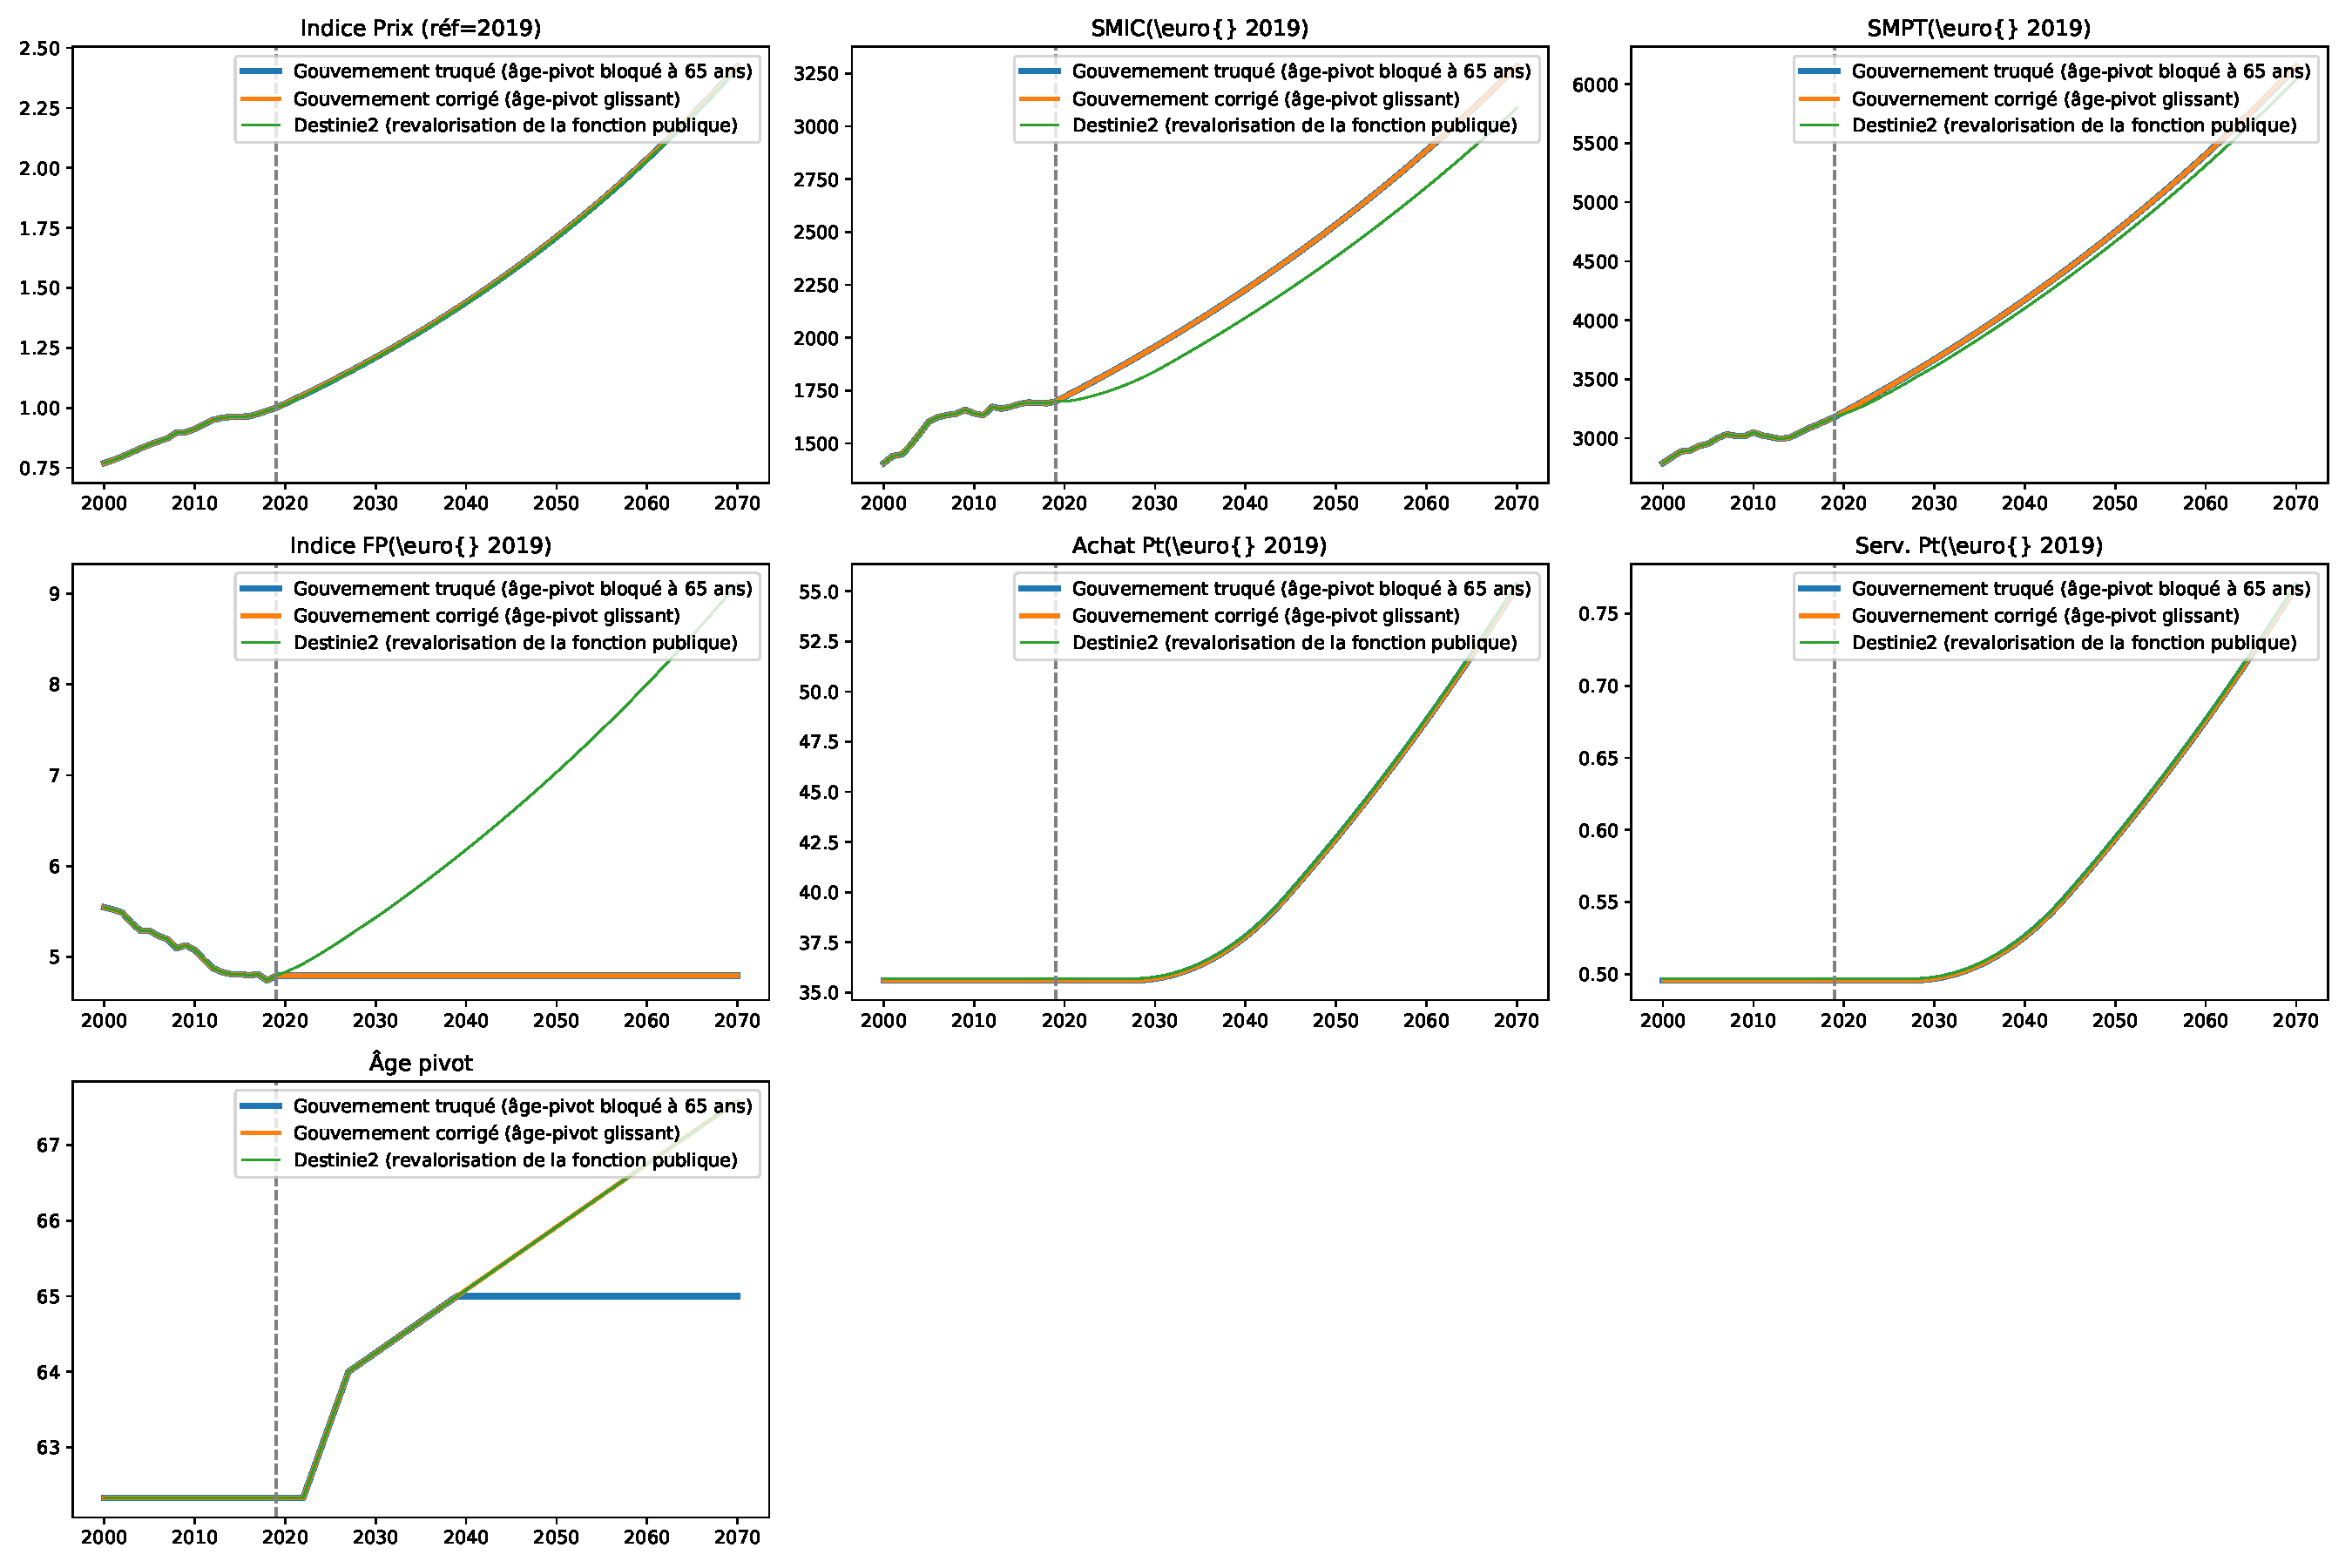
\includegraphics[width=1\textwidth]{fig/comparaison_modeles.pdf}\end{center} 

\newpage 
 
\chapter{Infirmière en soins généraux (CN, CS, puis HC)} 

\begin{minipage}{0.55\linewidth}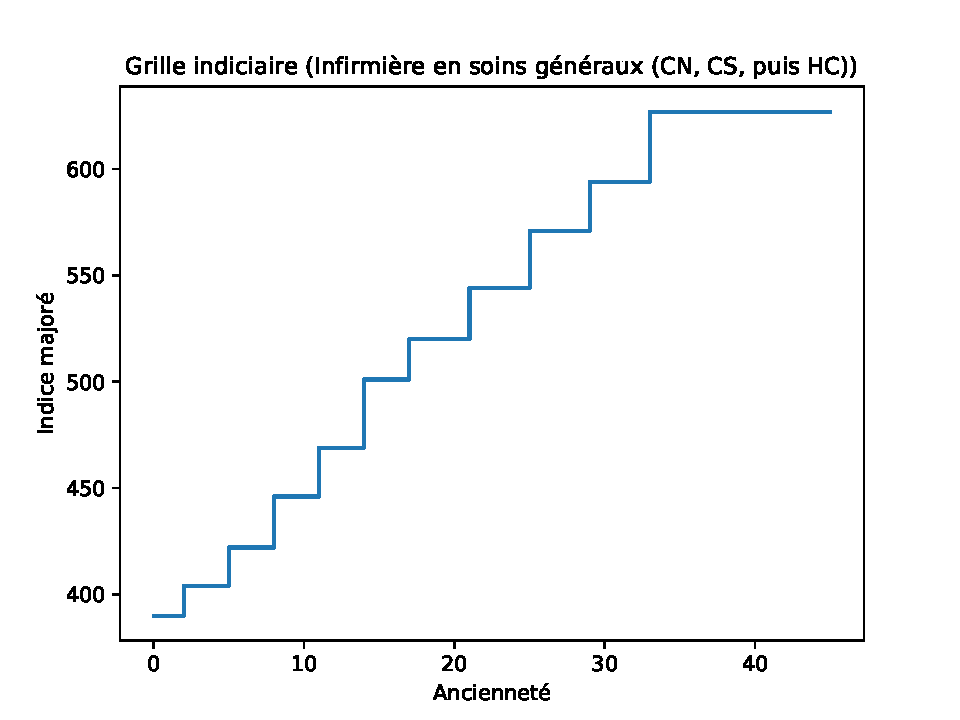
\includegraphics[width=0.7\textwidth]{fig/grille_Infirmier.pdf}\end{minipage} 
\begin{minipage}{0.3\linewidth} 
 \begin{center} 

\begin{tabular}[htb]{|c|c|} 
\hline 
 Indice majoré &  Durée (années) \\ 
\hline \hline 
 390 &  2.00 \\ 
\hline 
 404 &  3.00 \\ 
\hline 
 422 &  3.00 \\ 
\hline 
 446 &  3.00 \\ 
\hline 
 469 &  3.00 \\ 
\hline 
 501 &  3.00 \\ 
\hline 
 520 &  4.00 \\ 
\hline 
 544 &  4.00 \\ 
\hline 
 571 &  4.00 \\ 
\hline 
 594 &  4.00 \\ 
\hline 
 627 &   \\ 
\hline 
\hline 
\end{tabular} 
\end{center} 
 \end{minipage} 


 \addto{\captionsenglish}{ \renewcommand{\mtctitle}{}} \setcounter{minitocdepth}{2} 
 \minitoc \newpage 

\section{Début de carrière à 22 ans} 

\subsection{Génération 1975 (début en 1997)} 

\paragraph{Retraites possibles et ratios Revenu/SMIC à 70, 75, 80, 85, 90 ans avec le modèle \emph{Gouvernement truqué (âge-pivot bloqué à 65 ans)}}  
 
{ \scriptsize \begin{center} 
\begin{tabular}[htb]{|c|c||c|c||c|c||c||c|c|c|c|c|c|} 
\hline 
 Retraite en &  Âge &  Âge pivot &  Décote/Surcote &  Retraite (\euro{} 2019) &  Tx Rempl(\%) &  SMIC (\euro{} 2019) &  Retraite/SMIC &  Rev70/SMIC &  Rev75/SMIC &  Rev80/SMIC &  Rev85/SMIC &  Rev90/SMIC \\ 
\hline \hline 
 2037 &  62 &  64 ans 10 mois &  -14.17\% &  1636.88 &  {\bf 42.14} &  2143.00 &  {\bf {\color{red} 0.76}} &  {\bf {\color{red} 0.69}} &  {\bf {\color{red} 0.65}} &  {\bf {\color{red} 0.61}} &  {\bf {\color{red} 0.57}} &  {\bf {\color{red} 0.53}} \\ 
\hline 
 2038 &  63 &  64 ans 11 mois &  -9.58\% &  1786.41 &  {\bf 45.91} &  2170.86 &  {\bf {\color{red} 0.82}} &  {\bf {\color{red} 0.75}} &  {\bf {\color{red} 0.70}} &  {\bf {\color{red} 0.66}} &  {\bf {\color{red} 0.62}} &  {\bf {\color{red} 0.58}} \\ 
\hline 
 2039 &  64 &  65 ans 0 mois &  -5.00\% &  1944.26 &  {\bf 49.88} &  2199.08 &  {\bf {\color{red} 0.88}} &  {\bf {\color{red} 0.82}} &  {\bf {\color{red} 0.77}} &  {\bf {\color{red} 0.72}} &  {\bf {\color{red} 0.67}} &  {\bf {\color{red} 0.63}} \\ 
\hline 
 2040 &  65 &  65 ans 0 mois &  0.00\% &  2119.69 &  {\bf 54.28} &  2227.67 &  {\bf {\color{red} 0.95}} &  {\bf {\color{red} 0.89}} &  {\bf {\color{red} 0.84}} &  {\bf {\color{red} 0.78}} &  {\bf {\color{red} 0.73}} &  {\bf {\color{red} 0.69}} \\ 
\hline 
 2041 &  66 &  65 ans 0 mois &  5.00\% &  2304.94 &  {\bf 58.92} &  2256.63 &  {\bf 1.02} &  {\bf {\color{red} 0.97}} &  {\bf {\color{red} 0.91}} &  {\bf {\color{red} 0.85}} &  {\bf {\color{red} 0.80}} &  {\bf {\color{red} 0.75}} \\ 
\hline 
 2042 &  67 &  65 ans 0 mois &  10.00\% &  2500.52 &  {\bf 63.81} &  2285.97 &  {\bf 1.09} &  {\bf 1.05} &  {\bf {\color{red} 0.99}} &  {\bf {\color{red} 0.92}} &  {\bf {\color{red} 0.87}} &  {\bf {\color{red} 0.81}} \\ 
\hline 
\hline 
\end{tabular} 
\end{center} } 
\paragraph{Retraites possibles et ratios Revenu/SMIC à 70, 75, 80, 85, 90 ans avec le modèle \emph{Gouvernement corrigé (âge-pivot glissant)}}  
 
{ \scriptsize \begin{center} 
\begin{tabular}[htb]{|c|c||c|c||c|c||c||c|c|c|c|c|c|} 
\hline 
 Retraite en &  Âge &  Âge pivot &  Décote/Surcote &  Retraite (\euro{} 2019) &  Tx Rempl(\%) &  SMIC (\euro{} 2019) &  Retraite/SMIC &  Rev70/SMIC &  Rev75/SMIC &  Rev80/SMIC &  Rev85/SMIC &  Rev90/SMIC \\ 
\hline \hline 
 2037 &  62 &  64 ans 10 mois &  -14.17\% &  1636.88 &  {\bf 42.14} &  2143.00 &  {\bf {\color{red} 0.76}} &  {\bf {\color{red} 0.69}} &  {\bf {\color{red} 0.65}} &  {\bf {\color{red} 0.61}} &  {\bf {\color{red} 0.57}} &  {\bf {\color{red} 0.53}} \\ 
\hline 
 2038 &  63 &  64 ans 11 mois &  -9.58\% &  1786.41 &  {\bf 45.91} &  2170.86 &  {\bf {\color{red} 0.82}} &  {\bf {\color{red} 0.75}} &  {\bf {\color{red} 0.70}} &  {\bf {\color{red} 0.66}} &  {\bf {\color{red} 0.62}} &  {\bf {\color{red} 0.58}} \\ 
\hline 
 2039 &  64 &  65 ans 0 mois &  -5.00\% &  1944.26 &  {\bf 49.88} &  2199.08 &  {\bf {\color{red} 0.88}} &  {\bf {\color{red} 0.82}} &  {\bf {\color{red} 0.77}} &  {\bf {\color{red} 0.72}} &  {\bf {\color{red} 0.67}} &  {\bf {\color{red} 0.63}} \\ 
\hline 
 2040 &  65 &  65 ans 1 mois &  -0.42\% &  2110.86 &  {\bf 54.06} &  2227.67 &  {\bf {\color{red} 0.95}} &  {\bf {\color{red} 0.89}} &  {\bf {\color{red} 0.83}} &  {\bf {\color{red} 0.78}} &  {\bf {\color{red} 0.73}} &  {\bf {\color{red} 0.69}} \\ 
\hline 
 2041 &  66 &  65 ans 2 mois &  4.17\% &  2286.65 &  {\bf 58.45} &  2256.63 &  {\bf 1.01} &  {\bf {\color{red} 0.96}} &  {\bf {\color{red} 0.90}} &  {\bf {\color{red} 0.85}} &  {\bf {\color{red} 0.79}} &  {\bf {\color{red} 0.74}} \\ 
\hline 
 2042 &  67 &  65 ans 3 mois &  8.75\% &  2472.11 &  {\bf 63.08} &  2285.97 &  {\bf 1.08} &  {\bf 1.04} &  {\bf {\color{red} 0.98}} &  {\bf {\color{red} 0.91}} &  {\bf {\color{red} 0.86}} &  {\bf {\color{red} 0.80}} \\ 
\hline 
\hline 
\end{tabular} 
\end{center} } 
\paragraph{Retraites possibles et ratios Revenu/SMIC à 70, 75, 80, 85, 90 ans avec le modèle \emph{Destinie2 (revalorisation de la fonction publique)}}  
 
{ \scriptsize \begin{center} 
\begin{tabular}[htb]{|c|c||c|c||c|c||c||c|c|c|c|c|c|} 
\hline 
 Retraite en &  Âge &  Âge pivot &  Décote/Surcote &  Retraite (\euro{} 2019) &  Tx Rempl(\%) &  SMIC (\euro{} 2019) &  Retraite/SMIC &  Rev70/SMIC &  Rev75/SMIC &  Rev80/SMIC &  Rev85/SMIC &  Rev90/SMIC \\ 
\hline \hline 
 2037 &  62 &  64 ans 10 mois &  -14.17\% &  1802.13 &  {\bf 37.22} &  2014.82 &  {\bf {\color{red} 0.89}} &  {\bf {\color{red} 0.81}} &  {\bf {\color{red} 0.76}} &  {\bf {\color{red} 0.71}} &  {\bf {\color{red} 0.66}} &  {\bf {\color{red} 0.62}} \\ 
\hline 
 2038 &  63 &  64 ans 11 mois &  -9.58\% &  1974.56 &  {\bf 40.26} &  2041.01 &  {\bf {\color{red} 0.97}} &  {\bf {\color{red} 0.88}} &  {\bf {\color{red} 0.83}} &  {\bf {\color{red} 0.78}} &  {\bf {\color{red} 0.73}} &  {\bf {\color{red} 0.68}} \\ 
\hline 
 2039 &  64 &  65 ans 0 mois &  -5.00\% &  2157.77 &  {\bf 43.43} &  2067.55 &  {\bf 1.04} &  {\bf {\color{red} 0.97}} &  {\bf {\color{red} 0.91}} &  {\bf {\color{red} 0.85}} &  {\bf {\color{red} 0.80}} &  {\bf {\color{red} 0.75}} \\ 
\hline 
 2040 &  65 &  65 ans 1 mois &  -0.42\% &  2352.36 &  {\bf 46.74} &  2094.43 &  {\bf 1.12} &  {\bf 1.05} &  {\bf {\color{red} 0.99}} &  {\bf {\color{red} 0.93}} &  {\bf {\color{red} 0.87}} &  {\bf {\color{red} 0.81}} \\ 
\hline 
 2041 &  66 &  65 ans 2 mois &  4.17\% &  2558.98 &  {\bf 50.19} &  2121.65 &  {\bf 1.21} &  {\bf 1.15} &  {\bf 1.07} &  {\bf 1.01} &  {\bf {\color{red} 0.94}} &  {\bf {\color{red} 0.88}} \\ 
\hline 
 2042 &  67 &  65 ans 3 mois &  8.75\% &  2778.33 &  {\bf 53.79} &  2149.23 &  {\bf 1.29} &  {\bf 1.24} &  {\bf 1.17} &  {\bf 1.09} &  {\bf 1.02} &  {\bf {\color{red} 0.96}} \\ 
\hline 
\hline 
\end{tabular} 
\end{center} } 

 \begin{center}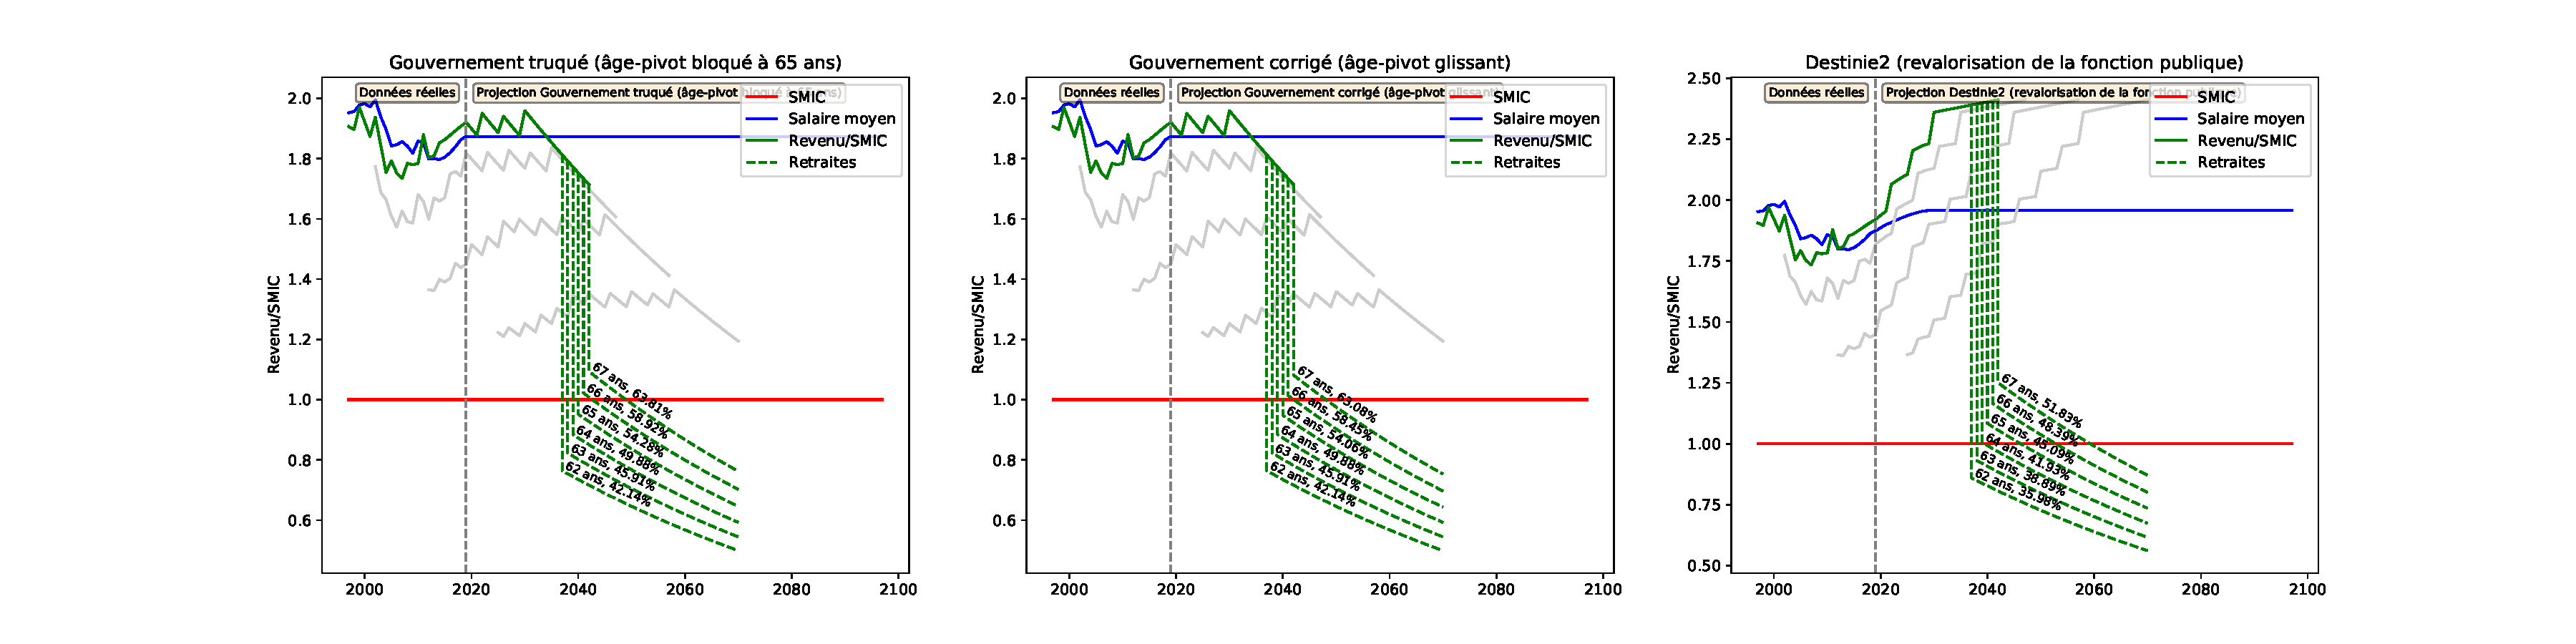
\includegraphics[width=0.9\textwidth]{fig/Infirmier_1975_22_dest_retraite.pdf}\end{center} \label{fig/Infirmier_1975_22_dest_retraite.pdf} 

\newpage 
 
\subsection{Génération 1980 (début en 2002)} 

\paragraph{Retraites possibles et ratios Revenu/SMIC à 70, 75, 80, 85, 90 ans avec le modèle \emph{Gouvernement truqué (âge-pivot bloqué à 65 ans)}}  
 
{ \scriptsize \begin{center} 
\begin{tabular}[htb]{|c|c||c|c||c|c||c||c|c|c|c|c|c|} 
\hline 
 Retraite en &  Âge &  Âge pivot &  Décote/Surcote &  Retraite (\euro{} 2019) &  Tx Rempl(\%) &  SMIC (\euro{} 2019) &  Retraite/SMIC &  Rev70/SMIC &  Rev75/SMIC &  Rev80/SMIC &  Rev85/SMIC &  Rev90/SMIC \\ 
\hline \hline 
 2042 &  62 &  65 ans 0 mois &  -15.00\% &  1654.36 &  {\bf 42.59} &  2285.97 &  {\bf {\color{red} 0.72}} &  {\bf {\color{red} 0.65}} &  {\bf {\color{red} 0.61}} &  {\bf {\color{red} 0.57}} &  {\bf {\color{red} 0.54}} &  {\bf {\color{red} 0.50}} \\ 
\hline 
 2043 &  63 &  65 ans 0 mois &  -10.00\% &  1820.50 &  {\bf 46.79} &  2315.68 &  {\bf {\color{red} 0.79}} &  {\bf {\color{red} 0.72}} &  {\bf {\color{red} 0.67}} &  {\bf {\color{red} 0.63}} &  {\bf {\color{red} 0.59}} &  {\bf {\color{red} 0.55}} \\ 
\hline 
 2044 &  64 &  65 ans 0 mois &  -5.00\% &  1996.69 &  {\bf 51.22} &  2345.79 &  {\bf {\color{red} 0.85}} &  {\bf {\color{red} 0.79}} &  {\bf {\color{red} 0.74}} &  {\bf {\color{red} 0.69}} &  {\bf {\color{red} 0.65}} &  {\bf {\color{red} 0.61}} \\ 
\hline 
 2045 &  65 &  65 ans 0 mois &  0.00\% &  2183.46 &  {\bf 55.92} &  2376.28 &  {\bf {\color{red} 0.92}} &  {\bf {\color{red} 0.86}} &  {\bf {\color{red} 0.81}} &  {\bf {\color{red} 0.76}} &  {\bf {\color{red} 0.71}} &  {\bf {\color{red} 0.67}} \\ 
\hline 
 2046 &  66 &  65 ans 0 mois &  5.00\% &  2379.61 &  {\bf 60.83} &  2407.18 &  {\bf {\color{red} 0.99}} &  {\bf {\color{red} 0.94}} &  {\bf {\color{red} 0.88}} &  {\bf {\color{red} 0.83}} &  {\bf {\color{red} 0.77}} &  {\bf {\color{red} 0.73}} \\ 
\hline 
 2047 &  67 &  65 ans 0 mois &  10.00\% &  2585.33 &  {\bf 65.97} &  2438.47 &  {\bf 1.06} &  {\bf 1.02} &  {\bf {\color{red} 0.96}} &  {\bf {\color{red} 0.90}} &  {\bf {\color{red} 0.84}} &  {\bf {\color{red} 0.79}} \\ 
\hline 
\hline 
\end{tabular} 
\end{center} } 
\paragraph{Retraites possibles et ratios Revenu/SMIC à 70, 75, 80, 85, 90 ans avec le modèle \emph{Gouvernement corrigé (âge-pivot glissant)}}  
 
{ \scriptsize \begin{center} 
\begin{tabular}[htb]{|c|c||c|c||c|c||c||c|c|c|c|c|c|} 
\hline 
 Retraite en &  Âge &  Âge pivot &  Décote/Surcote &  Retraite (\euro{} 2019) &  Tx Rempl(\%) &  SMIC (\euro{} 2019) &  Retraite/SMIC &  Rev70/SMIC &  Rev75/SMIC &  Rev80/SMIC &  Rev85/SMIC &  Rev90/SMIC \\ 
\hline \hline 
 2042 &  62 &  65 ans 3 mois &  -16.25\% &  1630.03 &  {\bf 41.97} &  2285.97 &  {\bf {\color{red} 0.71}} &  {\bf {\color{red} 0.64}} &  {\bf {\color{red} 0.60}} &  {\bf {\color{red} 0.57}} &  {\bf {\color{red} 0.53}} &  {\bf {\color{red} 0.50}} \\ 
\hline 
 2043 &  63 &  65 ans 4 mois &  -11.67\% &  1786.79 &  {\bf 45.92} &  2315.68 &  {\bf {\color{red} 0.77}} &  {\bf {\color{red} 0.70}} &  {\bf {\color{red} 0.66}} &  {\bf {\color{red} 0.62}} &  {\bf {\color{red} 0.58}} &  {\bf {\color{red} 0.54}} \\ 
\hline 
 2044 &  64 &  65 ans 5 mois &  -7.08\% &  1952.90 &  {\bf 50.10} &  2345.79 &  {\bf {\color{red} 0.83}} &  {\bf {\color{red} 0.77}} &  {\bf {\color{red} 0.72}} &  {\bf {\color{red} 0.68}} &  {\bf {\color{red} 0.63}} &  {\bf {\color{red} 0.60}} \\ 
\hline 
 2045 &  65 &  65 ans 6 mois &  -2.50\% &  2128.87 &  {\bf 54.52} &  2376.28 &  {\bf {\color{red} 0.90}} &  {\bf {\color{red} 0.84}} &  {\bf {\color{red} 0.79}} &  {\bf {\color{red} 0.74}} &  {\bf {\color{red} 0.69}} &  {\bf {\color{red} 0.65}} \\ 
\hline 
 2046 &  66 &  65 ans 7 mois &  2.08\% &  2313.50 &  {\bf 59.14} &  2407.18 &  {\bf {\color{red} 0.96}} &  {\bf {\color{red} 0.91}} &  {\bf {\color{red} 0.86}} &  {\bf {\color{red} 0.80}} &  {\bf {\color{red} 0.75}} &  {\bf {\color{red} 0.70}} \\ 
\hline 
 2047 &  67 &  65 ans 8 mois &  6.67\% &  2506.99 &  {\bf 63.97} &  2438.47 &  {\bf 1.03} &  {\bf {\color{red} 0.99}} &  {\bf {\color{red} 0.93}} &  {\bf {\color{red} 0.87}} &  {\bf {\color{red} 0.81}} &  {\bf {\color{red} 0.76}} \\ 
\hline 
\hline 
\end{tabular} 
\end{center} } 
\paragraph{Retraites possibles et ratios Revenu/SMIC à 70, 75, 80, 85, 90 ans avec le modèle \emph{Destinie2 (revalorisation de la fonction publique)}}  
 
{ \scriptsize \begin{center} 
\begin{tabular}[htb]{|c|c||c|c||c|c||c||c|c|c|c|c|c|} 
\hline 
 Retraite en &  Âge &  Âge pivot &  Décote/Surcote &  Retraite (\euro{} 2019) &  Tx Rempl(\%) &  SMIC (\euro{} 2019) &  Retraite/SMIC &  Rev70/SMIC &  Rev75/SMIC &  Rev80/SMIC &  Rev85/SMIC &  Rev90/SMIC \\ 
\hline \hline 
 2042 &  62 &  65 ans 3 mois &  -16.25\% &  1858.99 &  {\bf 35.99} &  2149.23 &  {\bf {\color{red} 0.86}} &  {\bf {\color{red} 0.78}} &  {\bf {\color{red} 0.73}} &  {\bf {\color{red} 0.69}} &  {\bf {\color{red} 0.64}} &  {\bf {\color{red} 0.60}} \\ 
\hline 
 2043 &  63 &  65 ans 4 mois &  -11.67\% &  2047.53 &  {\bf 39.13} &  2177.17 &  {\bf {\color{red} 0.94}} &  {\bf {\color{red} 0.86}} &  {\bf {\color{red} 0.81}} &  {\bf {\color{red} 0.76}} &  {\bf {\color{red} 0.71}} &  {\bf {\color{red} 0.66}} \\ 
\hline 
 2044 &  64 &  65 ans 5 mois &  -7.08\% &  2248.66 &  {\bf 42.43} &  2205.48 &  {\bf 1.02} &  {\bf {\color{red} 0.94}} &  {\bf {\color{red} 0.88}} &  {\bf {\color{red} 0.83}} &  {\bf {\color{red} 0.78}} &  {\bf {\color{red} 0.73}} \\ 
\hline 
 2045 &  65 &  65 ans 6 mois &  -2.50\% &  2463.12 &  {\bf 45.88} &  2234.15 &  {\bf 1.10} &  {\bf 1.03} &  {\bf {\color{red} 0.97}} &  {\bf {\color{red} 0.91}} &  {\bf {\color{red} 0.85}} &  {\bf {\color{red} 0.80}} \\ 
\hline 
 2046 &  66 &  65 ans 7 mois &  2.08\% &  2689.72 &  {\bf 49.45} &  2263.19 &  {\bf 1.19} &  {\bf 1.13} &  {\bf 1.06} &  {\bf {\color{red} 0.99}} &  {\bf {\color{red} 0.93}} &  {\bf {\color{red} 0.87}} \\ 
\hline 
 2047 &  67 &  65 ans 8 mois &  6.67\% &  2928.82 &  {\bf 53.16} &  2292.61 &  {\bf 1.28} &  {\bf 1.23} &  {\bf 1.15} &  {\bf 1.08} &  {\bf 1.01} &  {\bf {\color{red} 0.95}} \\ 
\hline 
\hline 
\end{tabular} 
\end{center} } 

 \begin{center}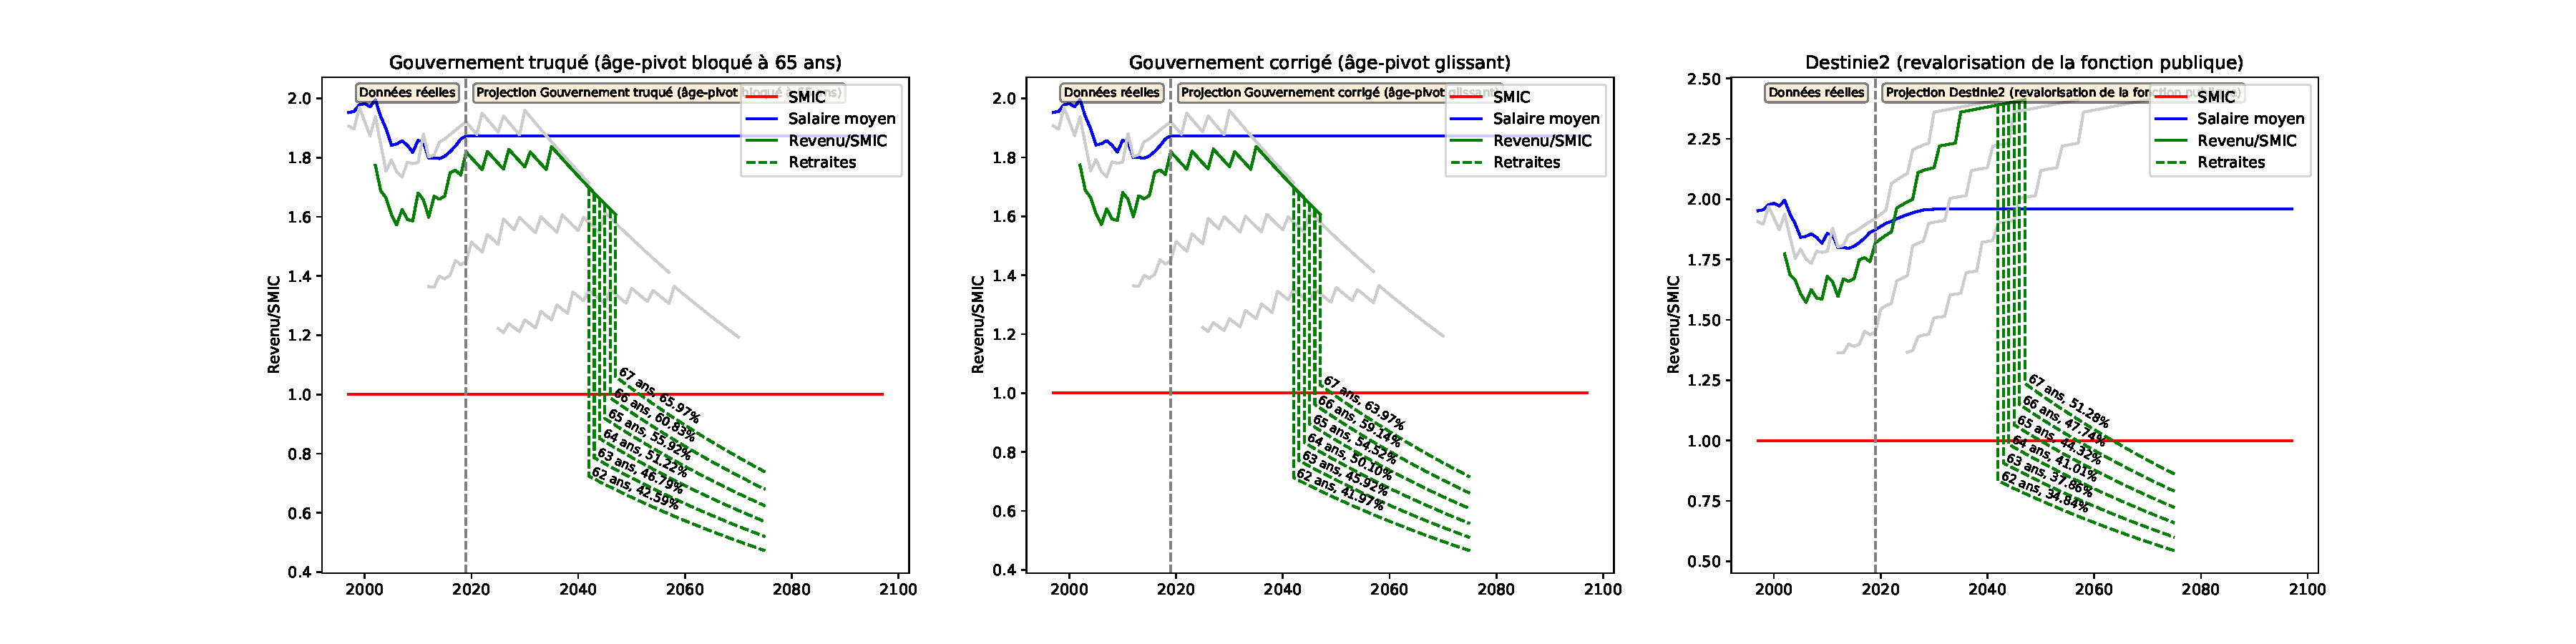
\includegraphics[width=0.9\textwidth]{fig/Infirmier_1980_22_dest_retraite.pdf}\end{center} \label{fig/Infirmier_1980_22_dest_retraite.pdf} 

\newpage 
 
\subsection{Génération 1990 (début en 2012)} 

\paragraph{Retraites possibles et ratios Revenu/SMIC à 70, 75, 80, 85, 90 ans avec le modèle \emph{Gouvernement truqué (âge-pivot bloqué à 65 ans)}}  
 
{ \scriptsize \begin{center} 
\begin{tabular}[htb]{|c|c||c|c||c|c||c||c|c|c|c|c|c|} 
\hline 
 Retraite en &  Âge &  Âge pivot &  Décote/Surcote &  Retraite (\euro{} 2019) &  Tx Rempl(\%) &  SMIC (\euro{} 2019) &  Retraite/SMIC &  Rev70/SMIC &  Rev75/SMIC &  Rev80/SMIC &  Rev85/SMIC &  Rev90/SMIC \\ 
\hline \hline 
 2052 &  62 &  65 ans 0 mois &  -15.00\% &  1773.04 &  {\bf 45.65} &  2601.14 &  {\bf {\color{red} 0.68}} &  {\bf {\color{red} 0.61}} &  {\bf {\color{red} 0.58}} &  {\bf {\color{red} 0.54}} &  {\bf {\color{red} 0.51}} &  {\bf {\color{red} 0.47}} \\ 
\hline 
 2053 &  63 &  65 ans 0 mois &  -10.00\% &  1950.49 &  {\bf 50.13} &  2634.96 &  {\bf {\color{red} 0.74}} &  {\bf {\color{red} 0.68}} &  {\bf {\color{red} 0.63}} &  {\bf {\color{red} 0.59}} &  {\bf {\color{red} 0.56}} &  {\bf {\color{red} 0.52}} \\ 
\hline 
 2054 &  64 &  65 ans 0 mois &  -5.00\% &  2137.16 &  {\bf 54.83} &  2669.21 &  {\bf {\color{red} 0.80}} &  {\bf {\color{red} 0.74}} &  {\bf {\color{red} 0.69}} &  {\bf {\color{red} 0.65}} &  {\bf {\color{red} 0.61}} &  {\bf {\color{red} 0.57}} \\ 
\hline 
 2055 &  65 &  65 ans 0 mois &  0.00\% &  2333.24 &  {\bf 59.75} &  2703.91 &  {\bf {\color{red} 0.86}} &  {\bf {\color{red} 0.81}} &  {\bf {\color{red} 0.76}} &  {\bf {\color{red} 0.71}} &  {\bf {\color{red} 0.67}} &  {\bf {\color{red} 0.62}} \\ 
\hline 
 2056 &  66 &  65 ans 0 mois &  5.00\% &  2538.93 &  {\bf 64.90} &  2739.06 &  {\bf {\color{red} 0.93}} &  {\bf {\color{red} 0.88}} &  {\bf {\color{red} 0.83}} &  {\bf {\color{red} 0.77}} &  {\bf {\color{red} 0.73}} &  {\bf {\color{red} 0.68}} \\ 
\hline 
 2057 &  67 &  65 ans 0 mois &  10.00\% &  2754.41 &  {\bf 70.29} &  2774.67 &  {\bf {\color{red} 0.99}} &  {\bf {\color{red} 0.95}} &  {\bf {\color{red} 0.90}} &  {\bf {\color{red} 0.84}} &  {\bf {\color{red} 0.79}} &  {\bf {\color{red} 0.74}} \\ 
\hline 
\hline 
\end{tabular} 
\end{center} } 
\paragraph{Retraites possibles et ratios Revenu/SMIC à 70, 75, 80, 85, 90 ans avec le modèle \emph{Gouvernement corrigé (âge-pivot glissant)}}  
 
{ \scriptsize \begin{center} 
\begin{tabular}[htb]{|c|c||c|c||c|c||c||c|c|c|c|c|c|} 
\hline 
 Retraite en &  Âge &  Âge pivot &  Décote/Surcote &  Retraite (\euro{} 2019) &  Tx Rempl(\%) &  SMIC (\euro{} 2019) &  Retraite/SMIC &  Rev70/SMIC &  Rev75/SMIC &  Rev80/SMIC &  Rev85/SMIC &  Rev90/SMIC \\ 
\hline \hline 
 2052 &  62 &  66 ans 1 mois &  -20.42\% &  1660.06 &  {\bf 42.74} &  2601.14 &  {\bf {\color{red} 0.64}} &  {\bf {\color{red} 0.58}} &  {\bf {\color{red} 0.54}} &  {\bf {\color{red} 0.51}} &  {\bf {\color{red} 0.47}} &  {\bf {\color{red} 0.44}} \\ 
\hline 
 2053 &  63 &  66 ans 2 mois &  -15.83\% &  1824.07 &  {\bf 46.88} &  2634.96 &  {\bf {\color{red} 0.69}} &  {\bf {\color{red} 0.63}} &  {\bf {\color{red} 0.59}} &  {\bf {\color{red} 0.56}} &  {\bf {\color{red} 0.52}} &  {\bf {\color{red} 0.49}} \\ 
\hline 
 2054 &  64 &  66 ans 3 mois &  -11.25\% &  1996.56 &  {\bf 51.22} &  2669.21 &  {\bf {\color{red} 0.75}} &  {\bf {\color{red} 0.69}} &  {\bf {\color{red} 0.65}} &  {\bf {\color{red} 0.61}} &  {\bf {\color{red} 0.57}} &  {\bf {\color{red} 0.53}} \\ 
\hline 
 2055 &  65 &  66 ans 4 mois &  -6.67\% &  2298.33 &  {\bf 58.86} &  2703.91 &  {\bf {\color{red} 0.85}} &  {\bf {\color{red} 0.80}} &  {\bf {\color{red} 0.75}} &  {\bf {\color{red} 0.70}} &  {\bf {\color{red} 0.66}} &  {\bf {\color{red} 0.62}} \\ 
\hline 
 2056 &  66 &  66 ans 5 mois &  -2.08\% &  2367.65 &  {\bf 60.53} &  2739.06 &  {\bf {\color{red} 0.86}} &  {\bf {\color{red} 0.82}} &  {\bf {\color{red} 0.77}} &  {\bf {\color{red} 0.72}} &  {\bf {\color{red} 0.68}} &  {\bf {\color{red} 0.63}} \\ 
\hline 
 2057 &  67 &  66 ans 6 mois &  2.50\% &  2566.61 &  {\bf 65.50} &  2774.67 &  {\bf {\color{red} 0.93}} &  {\bf {\color{red} 0.89}} &  {\bf {\color{red} 0.83}} &  {\bf {\color{red} 0.78}} &  {\bf {\color{red} 0.73}} &  {\bf {\color{red} 0.69}} \\ 
\hline 
\hline 
\end{tabular} 
\end{center} } 
\paragraph{Retraites possibles et ratios Revenu/SMIC à 70, 75, 80, 85, 90 ans avec le modèle \emph{Destinie2 (revalorisation de la fonction publique)}}  
 
{ \scriptsize \begin{center} 
\begin{tabular}[htb]{|c|c||c|c||c|c||c||c|c|c|c|c|c|} 
\hline 
 Retraite en &  Âge &  Âge pivot &  Décote/Surcote &  Retraite (\euro{} 2019) &  Tx Rempl(\%) &  SMIC (\euro{} 2019) &  Retraite/SMIC &  Rev70/SMIC &  Rev75/SMIC &  Rev80/SMIC &  Rev85/SMIC &  Rev90/SMIC \\ 
\hline \hline 
 2052 &  62 &  66 ans 1 mois &  -20.42\% &  2076.85 &  {\bf 35.34} &  2445.56 &  {\bf {\color{red} 0.85}} &  {\bf {\color{red} 0.77}} &  {\bf {\color{red} 0.72}} &  {\bf {\color{red} 0.67}} &  {\bf {\color{red} 0.63}} &  {\bf {\color{red} 0.59}} \\ 
\hline 
 2053 &  63 &  66 ans 2 mois &  -15.83\% &  2294.77 &  {\bf 38.54} &  2477.35 &  {\bf {\color{red} 0.93}} &  {\bf {\color{red} 0.85}} &  {\bf {\color{red} 0.79}} &  {\bf {\color{red} 0.74}} &  {\bf {\color{red} 0.70}} &  {\bf {\color{red} 0.65}} \\ 
\hline 
 2054 &  64 &  66 ans 3 mois &  -11.25\% &  2525.69 &  {\bf 41.88} &  2509.56 &  {\bf 1.01} &  {\bf {\color{red} 0.93}} &  {\bf {\color{red} 0.87}} &  {\bf {\color{red} 0.82}} &  {\bf {\color{red} 0.77}} &  {\bf {\color{red} 0.72}} \\ 
\hline 
 2055 &  65 &  66 ans 4 mois &  -6.67\% &  2770.02 &  {\bf 45.34} &  2542.18 &  {\bf 1.09} &  {\bf 1.02} &  {\bf {\color{red} 0.96}} &  {\bf {\color{red} 0.90}} &  {\bf {\color{red} 0.84}} &  {\bf {\color{red} 0.79}} \\ 
\hline 
 2056 &  66 &  66 ans 5 mois &  -2.08\% &  3028.18 &  {\bf 48.93} &  2575.23 &  {\bf 1.18} &  {\bf 1.12} &  {\bf 1.05} &  {\bf {\color{red} 0.98}} &  {\bf {\color{red} 0.92}} &  {\bf {\color{red} 0.86}} \\ 
\hline 
 2057 &  67 &  66 ans 6 mois &  2.50\% &  3300.58 &  {\bf 52.65} &  2608.71 &  {\bf 1.27} &  {\bf 1.22} &  {\bf 1.14} &  {\bf 1.07} &  {\bf 1.00} &  {\bf {\color{red} 0.94}} \\ 
\hline 
\hline 
\end{tabular} 
\end{center} } 

 \begin{center}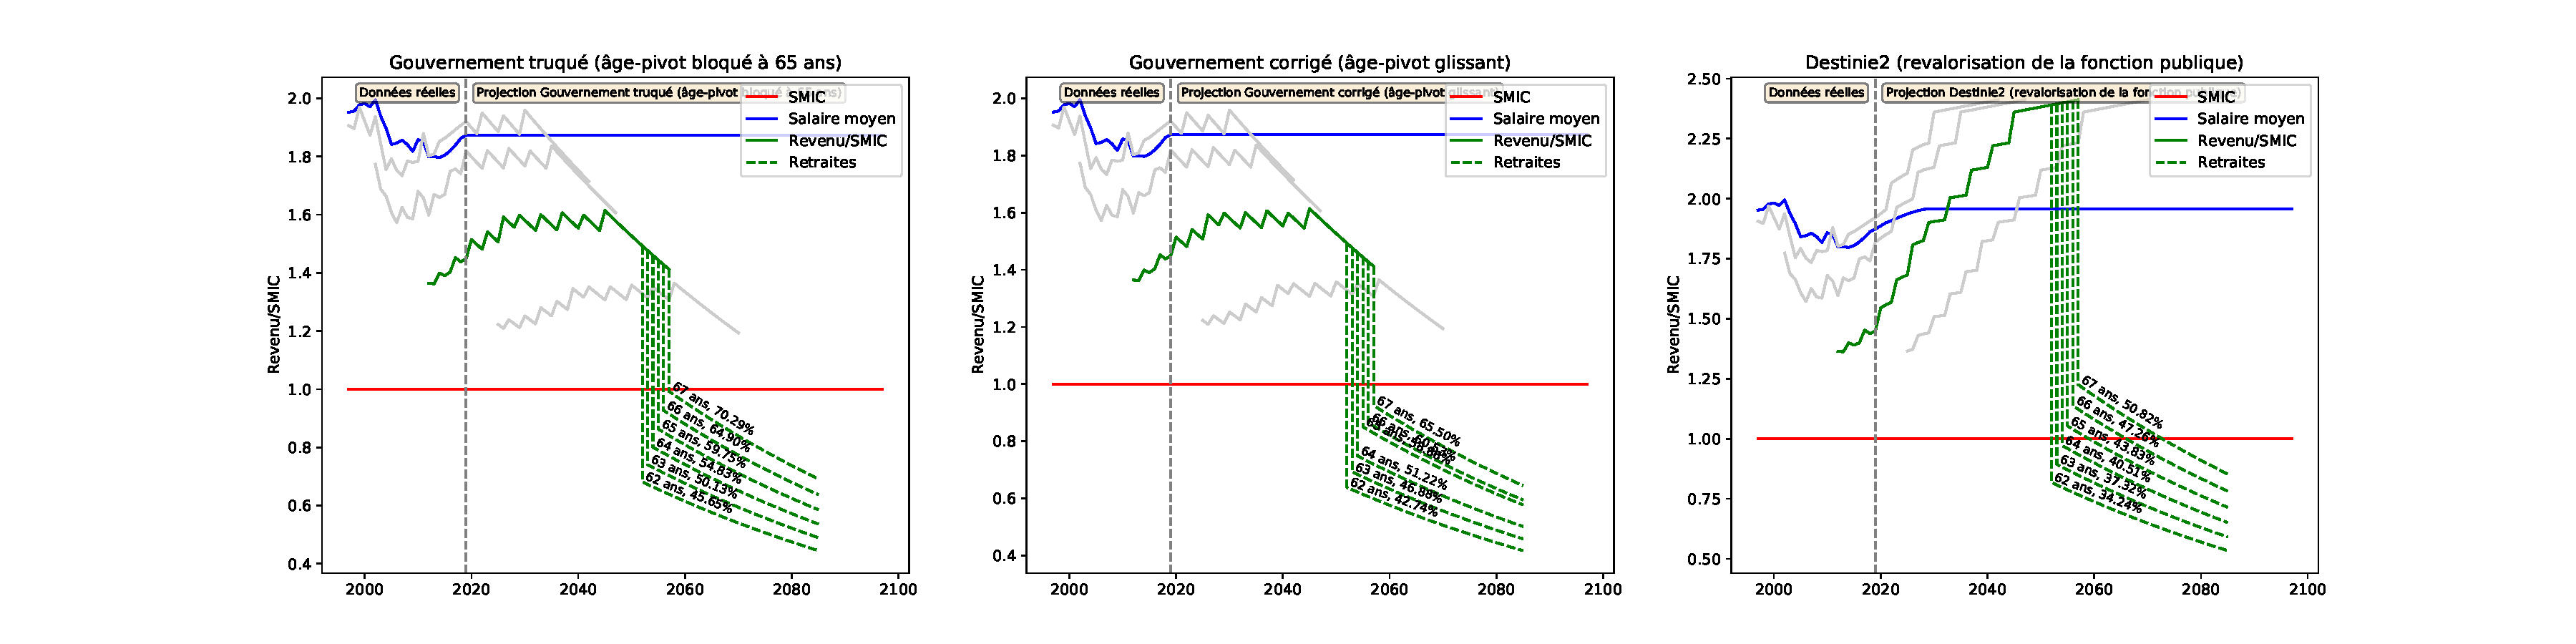
\includegraphics[width=0.9\textwidth]{fig/Infirmier_1990_22_dest_retraite.pdf}\end{center} \label{fig/Infirmier_1990_22_dest_retraite.pdf} 

\newpage 
 
\subsection{Génération 2003 (début en 2025)} 

\paragraph{Retraites possibles et ratios Revenu/SMIC à 70, 75, 80, 85, 90 ans avec le modèle \emph{Gouvernement truqué (âge-pivot bloqué à 65 ans)}}  
 
{ \scriptsize \begin{center} 
\begin{tabular}[htb]{|c|c||c|c||c|c||c||c|c|c|c|c|c|} 
\hline 
 Retraite en &  Âge &  Âge pivot &  Décote/Surcote &  Retraite (\euro{} 2019) &  Tx Rempl(\%) &  SMIC (\euro{} 2019) &  Retraite/SMIC &  Rev70/SMIC &  Rev75/SMIC &  Rev80/SMIC &  Rev85/SMIC &  Rev90/SMIC \\ 
\hline \hline 
 2065 &  62 &  65 ans 0 mois &  -15.00\% &  1896.25 &  {\bf 48.82} &  3076.71 &  {\bf {\color{red} 0.62}} &  {\bf {\color{red} 0.56}} &  {\bf {\color{red} 0.52}} &  {\bf {\color{red} 0.49}} &  {\bf {\color{red} 0.46}} &  {\bf {\color{red} 0.43}} \\ 
\hline 
 2066 &  63 &  65 ans 0 mois &  -10.00\% &  2082.64 &  {\bf 53.52} &  3116.71 &  {\bf {\color{red} 0.67}} &  {\bf {\color{red} 0.61}} &  {\bf {\color{red} 0.57}} &  {\bf {\color{red} 0.54}} &  {\bf {\color{red} 0.50}} &  {\bf {\color{red} 0.47}} \\ 
\hline 
 2067 &  64 &  65 ans 0 mois &  -5.00\% &  2278.46 &  {\bf 58.45} &  3157.23 &  {\bf {\color{red} 0.72}} &  {\bf {\color{red} 0.67}} &  {\bf {\color{red} 0.63}} &  {\bf {\color{red} 0.59}} &  {\bf {\color{red} 0.55}} &  {\bf {\color{red} 0.52}} \\ 
\hline 
 2068 &  65 &  65 ans 0 mois &  0.00\% &  2718.53 &  {\bf 69.62} &  3198.27 &  {\bf {\color{red} 0.85}} &  {\bf {\color{red} 0.80}} &  {\bf {\color{red} 0.75}} &  {\bf {\color{red} 0.70}} &  {\bf {\color{red} 0.66}} &  {\bf {\color{red} 0.62}} \\ 
\hline 
 2069 &  66 &  65 ans 0 mois &  5.00\% &  2753.87 &  {\bf 70.40} &  3239.85 &  {\bf {\color{red} 0.85}} &  {\bf {\color{red} 0.81}} &  {\bf {\color{red} 0.76}} &  {\bf {\color{red} 0.71}} &  {\bf {\color{red} 0.67}} &  {\bf {\color{red} 0.62}} \\ 
\hline 
 2070 &  67 &  65 ans 0 mois &  10.00\% &  2924.48 &  {\bf 74.63} &  3281.97 &  {\bf {\color{red} 0.89}} &  {\bf {\color{red} 0.86}} &  {\bf {\color{red} 0.80}} &  {\bf {\color{red} 0.75}} &  {\bf {\color{red} 0.71}} &  {\bf {\color{red} 0.66}} \\ 
\hline 
\hline 
\end{tabular} 
\end{center} } 
\paragraph{Retraites possibles et ratios Revenu/SMIC à 70, 75, 80, 85, 90 ans avec le modèle \emph{Gouvernement corrigé (âge-pivot glissant)}}  
 
{ \scriptsize \begin{center} 
\begin{tabular}[htb]{|c|c||c|c||c|c||c||c|c|c|c|c|c|} 
\hline 
 Retraite en &  Âge &  Âge pivot &  Décote/Surcote &  Retraite (\euro{} 2019) &  Tx Rempl(\%) &  SMIC (\euro{} 2019) &  Retraite/SMIC &  Rev70/SMIC &  Rev75/SMIC &  Rev80/SMIC &  Rev85/SMIC &  Rev90/SMIC \\ 
\hline \hline 
 2065 &  62 &  67 ans 2 mois &  -25.83\% &  1654.57 &  {\bf 42.60} &  3076.71 &  {\bf {\color{red} 0.54}} &  {\bf {\color{red} 0.48}} &  {\bf {\color{red} 0.45}} &  {\bf {\color{red} 0.43}} &  {\bf {\color{red} 0.40}} &  {\bf {\color{red} 0.37}} \\ 
\hline 
 2066 &  63 &  67 ans 3 mois &  -21.25\% &  1822.31 &  {\bf 46.83} &  3116.71 &  {\bf {\color{red} 0.58}} &  {\bf {\color{red} 0.53}} &  {\bf {\color{red} 0.50}} &  {\bf {\color{red} 0.47}} &  {\bf {\color{red} 0.44}} &  {\bf {\color{red} 0.41}} \\ 
\hline 
 2067 &  64 &  67 ans 4 mois &  -16.67\% &  1998.65 &  {\bf 51.27} &  3157.23 &  {\bf {\color{red} 0.63}} &  {\bf {\color{red} 0.59}} &  {\bf {\color{red} 0.55}} &  {\bf {\color{red} 0.51}} &  {\bf {\color{red} 0.48}} &  {\bf {\color{red} 0.45}} \\ 
\hline 
 2068 &  65 &  67 ans 5 mois &  -12.08\% &  2718.53 &  {\bf 69.62} &  3198.27 &  {\bf {\color{red} 0.85}} &  {\bf {\color{red} 0.80}} &  {\bf {\color{red} 0.75}} &  {\bf {\color{red} 0.70}} &  {\bf {\color{red} 0.66}} &  {\bf {\color{red} 0.62}} \\ 
\hline 
 2069 &  66 &  67 ans 6 mois &  -7.50\% &  2753.87 &  {\bf 70.40} &  3239.85 &  {\bf {\color{red} 0.85}} &  {\bf {\color{red} 0.81}} &  {\bf {\color{red} 0.76}} &  {\bf {\color{red} 0.71}} &  {\bf {\color{red} 0.67}} &  {\bf {\color{red} 0.62}} \\ 
\hline 
 2070 &  67 &  67 ans 7 mois &  -2.92\% &  2789.67 &  {\bf 71.19} &  3281.97 &  {\bf {\color{red} 0.85}} &  {\bf {\color{red} 0.82}} &  {\bf {\color{red} 0.77}} &  {\bf {\color{red} 0.72}} &  {\bf {\color{red} 0.67}} &  {\bf {\color{red} 0.63}} \\ 
\hline 
\hline 
\end{tabular} 
\end{center} } 
\paragraph{Retraites possibles et ratios Revenu/SMIC à 70, 75, 80, 85, 90 ans avec le modèle \emph{Destinie2 (revalorisation de la fonction publique)}}  
 
{ \scriptsize \begin{center} 
\begin{tabular}[htb]{|c|c||c|c||c|c||c||c|c|c|c|c|c|} 
\hline 
 Retraite en &  Âge &  Âge pivot &  Décote/Surcote &  Retraite (\euro{} 2019) &  Tx Rempl(\%) &  SMIC (\euro{} 2019) &  Retraite/SMIC &  Rev70/SMIC &  Rev75/SMIC &  Rev80/SMIC &  Rev85/SMIC &  Rev90/SMIC \\ 
\hline \hline 
 2065 &  62 &  67 ans 2 mois &  -25.83\% &  2408.18 &  {\bf 34.64} &  2892.68 &  {\bf {\color{red} 0.83}} &  {\bf {\color{red} 0.75}} &  {\bf {\color{red} 0.70}} &  {\bf {\color{red} 0.66}} &  {\bf {\color{red} 0.62}} &  {\bf {\color{red} 0.58}} \\ 
\hline 
 2066 &  63 &  67 ans 3 mois &  -21.25\% &  2667.43 &  {\bf 37.88} &  2930.29 &  {\bf {\color{red} 0.91}} &  {\bf {\color{red} 0.83}} &  {\bf {\color{red} 0.78}} &  {\bf {\color{red} 0.73}} &  {\bf {\color{red} 0.69}} &  {\bf {\color{red} 0.64}} \\ 
\hline 
 2067 &  64 &  67 ans 4 mois &  -16.67\% &  2942.12 &  {\bf 41.24} &  2968.38 &  {\bf {\color{red} 0.99}} &  {\bf {\color{red} 0.92}} &  {\bf {\color{red} 0.86}} &  {\bf {\color{red} 0.81}} &  {\bf {\color{red} 0.76}} &  {\bf {\color{red} 0.71}} \\ 
\hline 
 2068 &  65 &  67 ans 5 mois &  -12.08\% &  3232.72 &  {\bf 44.74} &  3006.97 &  {\bf 1.08} &  {\bf 1.01} &  {\bf {\color{red} 0.94}} &  {\bf {\color{red} 0.89}} &  {\bf {\color{red} 0.83}} &  {\bf {\color{red} 0.78}} \\ 
\hline 
 2069 &  66 &  67 ans 6 mois &  -7.50\% &  3539.72 &  {\bf 48.35} &  3046.06 &  {\bf 1.16} &  {\bf 1.10} &  {\bf 1.03} &  {\bf {\color{red} 0.97}} &  {\bf {\color{red} 0.91}} &  {\bf {\color{red} 0.85}} \\ 
\hline 
 2070 &  67 &  67 ans 7 mois &  -2.92\% &  3863.61 &  {\bf 52.10} &  3085.66 &  {\bf 1.25} &  {\bf 1.20} &  {\bf 1.13} &  {\bf 1.06} &  {\bf {\color{red} 0.99}} &  {\bf {\color{red} 0.93}} \\ 
\hline 
\hline 
\end{tabular} 
\end{center} } 

 \begin{center}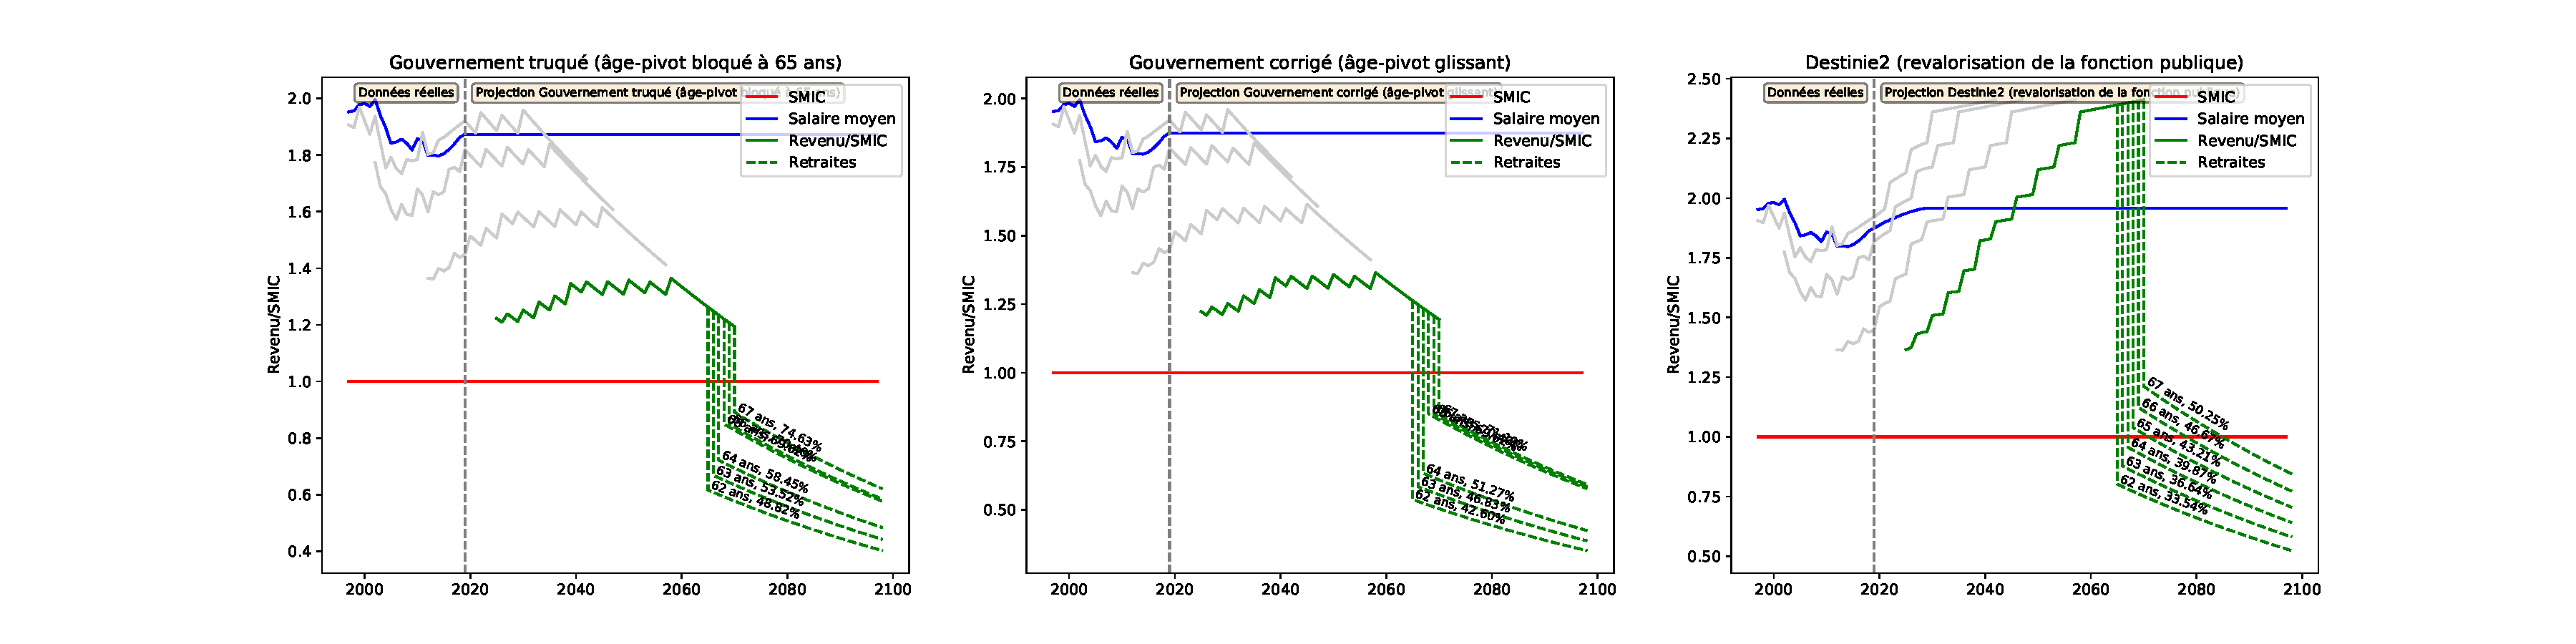
\includegraphics[width=0.9\textwidth]{fig/Infirmier_2003_22_dest_retraite.pdf}\end{center} \label{fig/Infirmier_2003_22_dest_retraite.pdf} 

\newpage 
 
\chapter{Aide-soignante (CN puis HC)} 

\begin{minipage}{0.55\linewidth}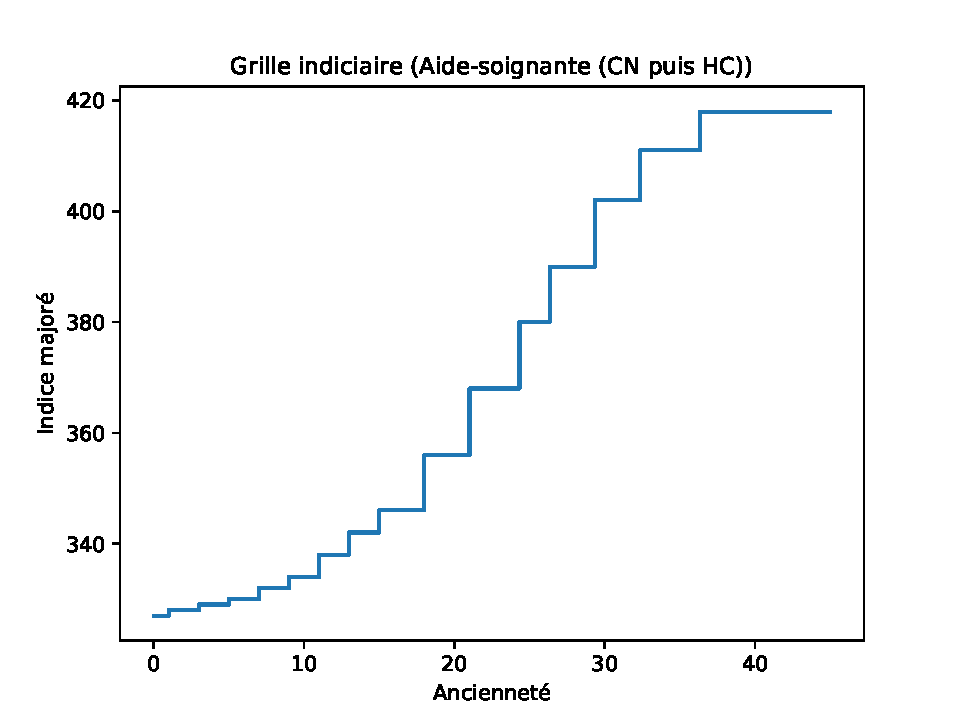
\includegraphics[width=0.7\textwidth]{fig/grille_AideSoignant.pdf}\end{minipage} 
\begin{minipage}{0.3\linewidth} 
 \begin{center} 

\begin{tabular}[htb]{|c|c|} 
\hline 
 Indice majoré &  Durée (années) \\ 
\hline \hline 
 327 &  1.00 \\ 
\hline 
 328 &  2.00 \\ 
\hline 
 329 &  2.00 \\ 
\hline 
 330 &  2.00 \\ 
\hline 
 332 &  2.00 \\ 
\hline 
 334 &  2.00 \\ 
\hline 
 338 &  2.00 \\ 
\hline 
 342 &  2.00 \\ 
\hline 
 346 &  3.00 \\ 
\hline 
 356 &  3.00 \\ 
\hline 
 368 &  3.33 \\ 
\hline 
 380 &  2.00 \\ 
\hline 
 390 &  3.00 \\ 
\hline 
 402 &  3.00 \\ 
\hline 
 411 &  4.00 \\ 
\hline 
 418 &   \\ 
\hline 
\hline 
\end{tabular} 
\end{center} 
 \end{minipage} 


 \addto{\captionsenglish}{ \renewcommand{\mtctitle}{}} \setcounter{minitocdepth}{2} 
 \minitoc \newpage 

\section{Début de carrière à 22 ans} 

\subsection{Génération 1975 (début en 1997)} 

\paragraph{Retraites possibles et ratios Revenu/SMIC à 70, 75, 80, 85, 90 ans avec le modèle \emph{Gouvernement truqué (âge-pivot bloqué à 65 ans)}}  
 
{ \scriptsize \begin{center} 
\begin{tabular}[htb]{|c|c||c|c||c|c||c||c|c|c|c|c|c|} 
\hline 
 Retraite en &  Âge &  Âge pivot &  Décote/Surcote &  Retraite (\euro{} 2019) &  Tx Rempl(\%) &  SMIC (\euro{} 2019) &  Retraite/SMIC &  Rev70/SMIC &  Rev75/SMIC &  Rev80/SMIC &  Rev85/SMIC &  Rev90/SMIC \\ 
\hline \hline 
 2037 &  62 &  64 ans 10 mois &  -14.17\% &  1111.54 &  {\bf 44.91} &  2143.00 &  {\bf {\color{red} 0.52}} &  {\bf {\color{red} 0.47}} &  {\bf {\color{red} 0.44}} &  {\bf {\color{red} 0.41}} &  {\bf {\color{red} 0.39}} &  {\bf {\color{red} 0.36}} \\ 
\hline 
 2038 &  63 &  64 ans 11 mois &  -9.58\% &  1211.04 &  {\bf 48.84} &  2170.86 &  {\bf {\color{red} 0.56}} &  {\bf {\color{red} 0.51}} &  {\bf {\color{red} 0.48}} &  {\bf {\color{red} 0.45}} &  {\bf {\color{red} 0.42}} &  {\bf {\color{red} 0.39}} \\ 
\hline 
 2039 &  64 &  65 ans 0 mois &  -5.00\% &  1315.96 &  {\bf 52.97} &  2199.08 &  {\bf {\color{red} 0.60}} &  {\bf {\color{red} 0.55}} &  {\bf {\color{red} 0.52}} &  {\bf {\color{red} 0.49}} &  {\bf {\color{red} 0.46}} &  {\bf {\color{red} 0.43}} \\ 
\hline 
 2040 &  65 &  65 ans 0 mois &  0.00\% &  1893.52 &  {\bf 76.07} &  2227.67 &  {\bf {\color{red} 0.85}} &  {\bf {\color{red} 0.80}} &  {\bf {\color{red} 0.75}} &  {\bf {\color{red} 0.70}} &  {\bf {\color{red} 0.66}} &  {\bf {\color{red} 0.62}} \\ 
\hline 
 2041 &  66 &  65 ans 0 mois &  5.00\% &  1918.14 &  {\bf 76.92} &  2256.63 &  {\bf {\color{red} 0.85}} &  {\bf {\color{red} 0.81}} &  {\bf {\color{red} 0.76}} &  {\bf {\color{red} 0.71}} &  {\bf {\color{red} 0.67}} &  {\bf {\color{red} 0.62}} \\ 
\hline 
 2042 &  67 &  65 ans 0 mois &  10.00\% &  1943.07 &  {\bf 77.78} &  2285.97 &  {\bf {\color{red} 0.85}} &  {\bf {\color{red} 0.82}} &  {\bf {\color{red} 0.77}} &  {\bf {\color{red} 0.72}} &  {\bf {\color{red} 0.67}} &  {\bf {\color{red} 0.63}} \\ 
\hline 
\hline 
\end{tabular} 
\end{center} } 
\paragraph{Retraites possibles et ratios Revenu/SMIC à 70, 75, 80, 85, 90 ans avec le modèle \emph{Gouvernement corrigé (âge-pivot glissant)}}  
 
{ \scriptsize \begin{center} 
\begin{tabular}[htb]{|c|c||c|c||c|c||c||c|c|c|c|c|c|} 
\hline 
 Retraite en &  Âge &  Âge pivot &  Décote/Surcote &  Retraite (\euro{} 2019) &  Tx Rempl(\%) &  SMIC (\euro{} 2019) &  Retraite/SMIC &  Rev70/SMIC &  Rev75/SMIC &  Rev80/SMIC &  Rev85/SMIC &  Rev90/SMIC \\ 
\hline \hline 
 2037 &  62 &  64 ans 10 mois &  -14.17\% &  1111.54 &  {\bf 44.91} &  2143.00 &  {\bf {\color{red} 0.52}} &  {\bf {\color{red} 0.47}} &  {\bf {\color{red} 0.44}} &  {\bf {\color{red} 0.41}} &  {\bf {\color{red} 0.39}} &  {\bf {\color{red} 0.36}} \\ 
\hline 
 2038 &  63 &  64 ans 11 mois &  -9.58\% &  1211.04 &  {\bf 48.84} &  2170.86 &  {\bf {\color{red} 0.56}} &  {\bf {\color{red} 0.51}} &  {\bf {\color{red} 0.48}} &  {\bf {\color{red} 0.45}} &  {\bf {\color{red} 0.42}} &  {\bf {\color{red} 0.39}} \\ 
\hline 
 2039 &  64 &  65 ans 0 mois &  -5.00\% &  1315.96 &  {\bf 52.97} &  2199.08 &  {\bf {\color{red} 0.60}} &  {\bf {\color{red} 0.55}} &  {\bf {\color{red} 0.52}} &  {\bf {\color{red} 0.49}} &  {\bf {\color{red} 0.46}} &  {\bf {\color{red} 0.43}} \\ 
\hline 
 2040 &  65 &  65 ans 1 mois &  -0.42\% &  1893.52 &  {\bf 76.07} &  2227.67 &  {\bf {\color{red} 0.85}} &  {\bf {\color{red} 0.80}} &  {\bf {\color{red} 0.75}} &  {\bf {\color{red} 0.70}} &  {\bf {\color{red} 0.66}} &  {\bf {\color{red} 0.62}} \\ 
\hline 
 2041 &  66 &  65 ans 2 mois &  4.17\% &  1918.14 &  {\bf 76.92} &  2256.63 &  {\bf {\color{red} 0.85}} &  {\bf {\color{red} 0.81}} &  {\bf {\color{red} 0.76}} &  {\bf {\color{red} 0.71}} &  {\bf {\color{red} 0.67}} &  {\bf {\color{red} 0.62}} \\ 
\hline 
 2042 &  67 &  65 ans 3 mois &  8.75\% &  1943.07 &  {\bf 77.78} &  2285.97 &  {\bf {\color{red} 0.85}} &  {\bf {\color{red} 0.82}} &  {\bf {\color{red} 0.77}} &  {\bf {\color{red} 0.72}} &  {\bf {\color{red} 0.67}} &  {\bf {\color{red} 0.63}} \\ 
\hline 
\hline 
\end{tabular} 
\end{center} } 
\paragraph{Retraites possibles et ratios Revenu/SMIC à 70, 75, 80, 85, 90 ans avec le modèle \emph{Destinie2 (revalorisation de la fonction publique)}}  
 
{ \scriptsize \begin{center} 
\begin{tabular}[htb]{|c|c||c|c||c|c||c||c|c|c|c|c|c|} 
\hline 
 Retraite en &  Âge &  Âge pivot &  Décote/Surcote &  Retraite (\euro{} 2019) &  Tx Rempl(\%) &  SMIC (\euro{} 2019) &  Retraite/SMIC &  Rev70/SMIC &  Rev75/SMIC &  Rev80/SMIC &  Rev85/SMIC &  Rev90/SMIC \\ 
\hline \hline 
 2037 &  62 &  64 ans 10 mois &  -14.17\% &  1232.66 &  {\bf 39.94} &  2014.82 &  {\bf {\color{red} 0.61}} &  {\bf {\color{red} 0.55}} &  {\bf {\color{red} 0.52}} &  {\bf {\color{red} 0.48}} &  {\bf {\color{red} 0.45}} &  {\bf {\color{red} 0.43}} \\ 
\hline 
 2038 &  63 &  64 ans 11 mois &  -9.58\% &  1347.73 &  {\bf 43.11} &  2041.01 &  {\bf {\color{red} 0.66}} &  {\bf {\color{red} 0.60}} &  {\bf {\color{red} 0.57}} &  {\bf {\color{red} 0.53}} &  {\bf {\color{red} 0.50}} &  {\bf {\color{red} 0.47}} \\ 
\hline 
 2039 &  64 &  65 ans 0 mois &  -5.00\% &  1469.81 &  {\bf 46.41} &  2067.55 &  {\bf {\color{red} 0.71}} &  {\bf {\color{red} 0.66}} &  {\bf {\color{red} 0.62}} &  {\bf {\color{red} 0.58}} &  {\bf {\color{red} 0.54}} &  {\bf {\color{red} 0.51}} \\ 
\hline 
 2040 &  65 &  65 ans 1 mois &  -0.42\% &  1780.26 &  {\bf 55.49} &  2094.43 &  {\bf {\color{red} 0.85}} &  {\bf {\color{red} 0.80}} &  {\bf {\color{red} 0.75}} &  {\bf {\color{red} 0.70}} &  {\bf {\color{red} 0.66}} &  {\bf {\color{red} 0.62}} \\ 
\hline 
 2041 &  66 &  65 ans 2 mois &  4.17\% &  1803.40 &  {\bf 55.49} &  2121.65 &  {\bf {\color{red} 0.85}} &  {\bf {\color{red} 0.81}} &  {\bf {\color{red} 0.76}} &  {\bf {\color{red} 0.71}} &  {\bf {\color{red} 0.67}} &  {\bf {\color{red} 0.62}} \\ 
\hline 
 2042 &  67 &  65 ans 3 mois &  8.75\% &  1882.28 &  {\bf 57.17} &  2149.23 &  {\bf {\color{red} 0.88}} &  {\bf {\color{red} 0.84}} &  {\bf {\color{red} 0.79}} &  {\bf {\color{red} 0.74}} &  {\bf {\color{red} 0.69}} &  {\bf {\color{red} 0.65}} \\ 
\hline 
\hline 
\end{tabular} 
\end{center} } 

 \begin{center}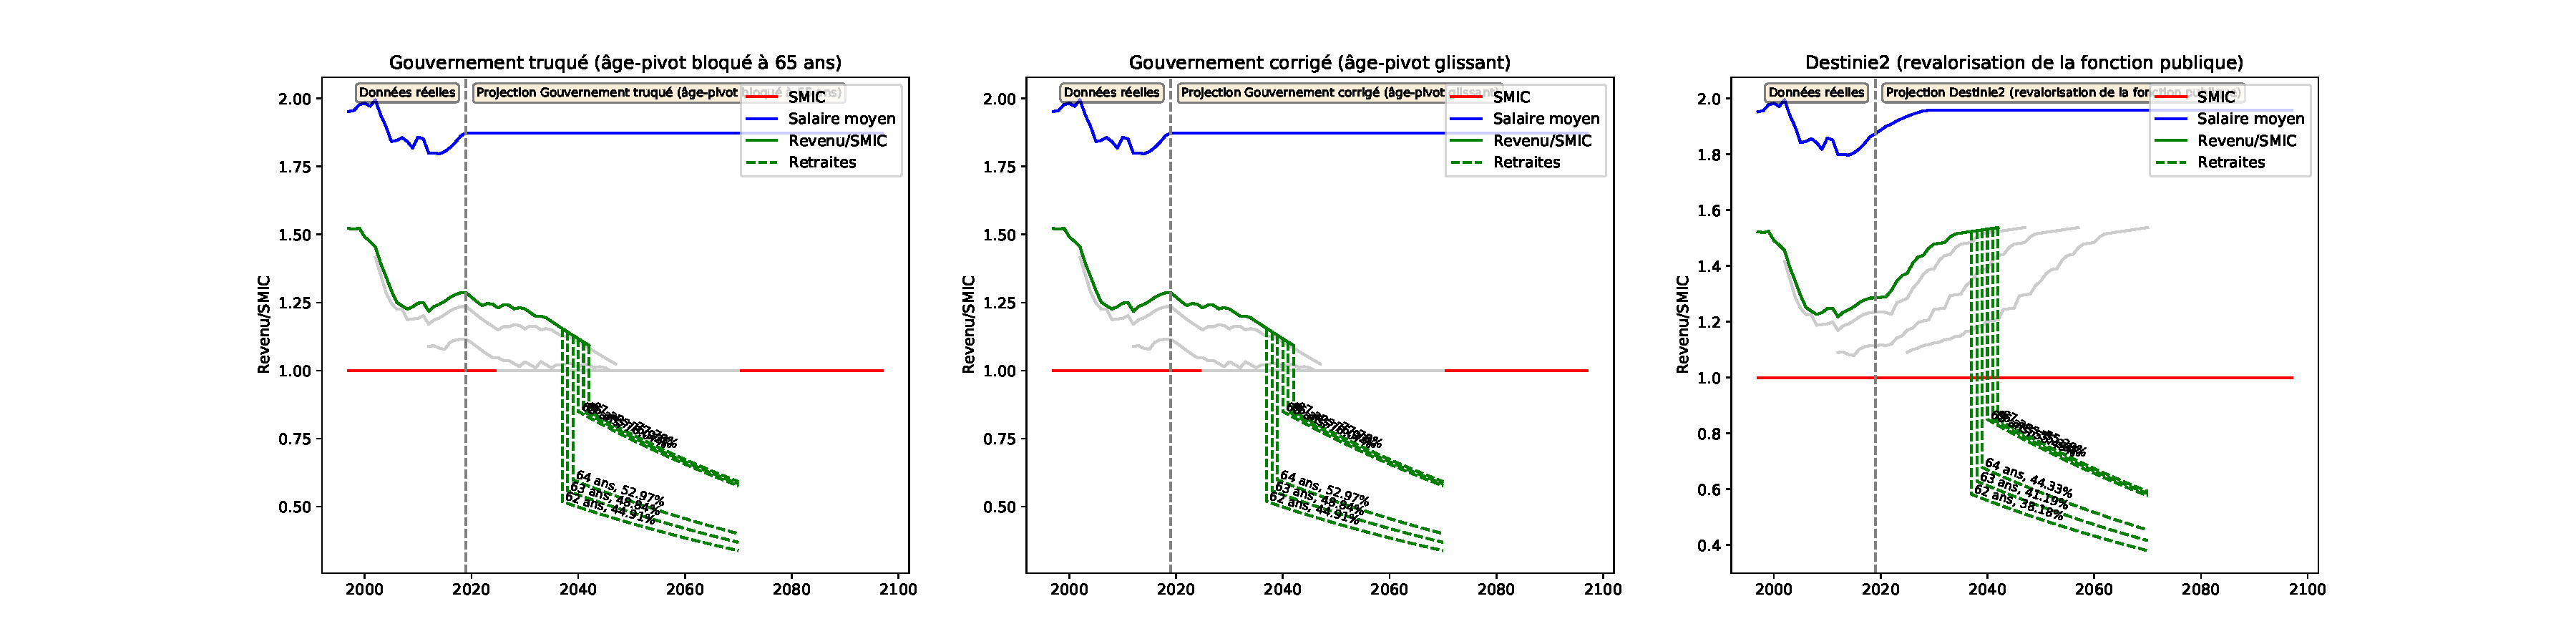
\includegraphics[width=0.9\textwidth]{fig/AideSoignant_1975_22_dest_retraite.pdf}\end{center} \label{fig/AideSoignant_1975_22_dest_retraite.pdf} 

\newpage 
 
\subsection{Génération 1980 (début en 2002)} 

\paragraph{Retraites possibles et ratios Revenu/SMIC à 70, 75, 80, 85, 90 ans avec le modèle \emph{Gouvernement truqué (âge-pivot bloqué à 65 ans)}}  
 
{ \scriptsize \begin{center} 
\begin{tabular}[htb]{|c|c||c|c||c|c||c||c|c|c|c|c|c|} 
\hline 
 Retraite en &  Âge &  Âge pivot &  Décote/Surcote &  Retraite (\euro{} 2019) &  Tx Rempl(\%) &  SMIC (\euro{} 2019) &  Retraite/SMIC &  Rev70/SMIC &  Rev75/SMIC &  Rev80/SMIC &  Rev85/SMIC &  Rev90/SMIC \\ 
\hline \hline 
 2042 &  62 &  65 ans 0 mois &  -15.00\% &  1124.91 &  {\bf 45.45} &  2285.97 &  {\bf {\color{red} 0.49}} &  {\bf {\color{red} 0.44}} &  {\bf {\color{red} 0.42}} &  {\bf {\color{red} 0.39}} &  {\bf {\color{red} 0.37}} &  {\bf {\color{red} 0.34}} \\ 
\hline 
 2043 &  63 &  65 ans 0 mois &  -10.00\% &  1235.80 &  {\bf 49.83} &  2315.68 &  {\bf {\color{red} 0.53}} &  {\bf {\color{red} 0.49}} &  {\bf {\color{red} 0.46}} &  {\bf {\color{red} 0.43}} &  {\bf {\color{red} 0.40}} &  {\bf {\color{red} 0.38}} \\ 
\hline 
 2044 &  64 &  65 ans 0 mois &  -5.00\% &  1353.27 &  {\bf 54.47} &  2345.79 &  {\bf {\color{red} 0.58}} &  {\bf {\color{red} 0.53}} &  {\bf {\color{red} 0.50}} &  {\bf {\color{red} 0.47}} &  {\bf {\color{red} 0.44}} &  {\bf {\color{red} 0.41}} \\ 
\hline 
 2045 &  65 &  65 ans 0 mois &  0.00\% &  2019.84 &  {\bf 81.15} &  2376.28 &  {\bf {\color{red} 0.85}} &  {\bf {\color{red} 0.80}} &  {\bf {\color{red} 0.75}} &  {\bf {\color{red} 0.70}} &  {\bf {\color{red} 0.66}} &  {\bf {\color{red} 0.62}} \\ 
\hline 
 2046 &  66 &  65 ans 0 mois &  5.00\% &  2046.10 &  {\bf 82.05} &  2407.18 &  {\bf {\color{red} 0.85}} &  {\bf {\color{red} 0.81}} &  {\bf {\color{red} 0.76}} &  {\bf {\color{red} 0.71}} &  {\bf {\color{red} 0.67}} &  {\bf {\color{red} 0.62}} \\ 
\hline 
 2047 &  67 &  65 ans 0 mois &  10.00\% &  2072.70 &  {\bf 82.97} &  2438.47 &  {\bf {\color{red} 0.85}} &  {\bf {\color{red} 0.82}} &  {\bf {\color{red} 0.77}} &  {\bf {\color{red} 0.72}} &  {\bf {\color{red} 0.67}} &  {\bf {\color{red} 0.63}} \\ 
\hline 
\hline 
\end{tabular} 
\end{center} } 
\paragraph{Retraites possibles et ratios Revenu/SMIC à 70, 75, 80, 85, 90 ans avec le modèle \emph{Gouvernement corrigé (âge-pivot glissant)}}  
 
{ \scriptsize \begin{center} 
\begin{tabular}[htb]{|c|c||c|c||c|c||c||c|c|c|c|c|c|} 
\hline 
 Retraite en &  Âge &  Âge pivot &  Décote/Surcote &  Retraite (\euro{} 2019) &  Tx Rempl(\%) &  SMIC (\euro{} 2019) &  Retraite/SMIC &  Rev70/SMIC &  Rev75/SMIC &  Rev80/SMIC &  Rev85/SMIC &  Rev90/SMIC \\ 
\hline \hline 
 2042 &  62 &  65 ans 3 mois &  -16.25\% &  1108.37 &  {\bf 44.78} &  2285.97 &  {\bf {\color{red} 0.48}} &  {\bf {\color{red} 0.44}} &  {\bf {\color{red} 0.41}} &  {\bf {\color{red} 0.38}} &  {\bf {\color{red} 0.36}} &  {\bf {\color{red} 0.34}} \\ 
\hline 
 2043 &  63 &  65 ans 4 mois &  -11.67\% &  1212.92 &  {\bf 48.91} &  2315.68 &  {\bf {\color{red} 0.52}} &  {\bf {\color{red} 0.48}} &  {\bf {\color{red} 0.45}} &  {\bf {\color{red} 0.42}} &  {\bf {\color{red} 0.39}} &  {\bf {\color{red} 0.37}} \\ 
\hline 
 2044 &  64 &  65 ans 5 mois &  -7.08\% &  1323.59 &  {\bf 53.28} &  2345.79 &  {\bf {\color{red} 0.56}} &  {\bf {\color{red} 0.52}} &  {\bf {\color{red} 0.49}} &  {\bf {\color{red} 0.46}} &  {\bf {\color{red} 0.43}} &  {\bf {\color{red} 0.40}} \\ 
\hline 
 2045 &  65 &  65 ans 6 mois &  -2.50\% &  2019.84 &  {\bf 81.15} &  2376.28 &  {\bf {\color{red} 0.85}} &  {\bf {\color{red} 0.80}} &  {\bf {\color{red} 0.75}} &  {\bf {\color{red} 0.70}} &  {\bf {\color{red} 0.66}} &  {\bf {\color{red} 0.62}} \\ 
\hline 
 2046 &  66 &  65 ans 7 mois &  2.08\% &  2046.10 &  {\bf 82.05} &  2407.18 &  {\bf {\color{red} 0.85}} &  {\bf {\color{red} 0.81}} &  {\bf {\color{red} 0.76}} &  {\bf {\color{red} 0.71}} &  {\bf {\color{red} 0.67}} &  {\bf {\color{red} 0.62}} \\ 
\hline 
 2047 &  67 &  65 ans 8 mois &  6.67\% &  2072.70 &  {\bf 82.97} &  2438.47 &  {\bf {\color{red} 0.85}} &  {\bf {\color{red} 0.82}} &  {\bf {\color{red} 0.77}} &  {\bf {\color{red} 0.72}} &  {\bf {\color{red} 0.67}} &  {\bf {\color{red} 0.63}} \\ 
\hline 
\hline 
\end{tabular} 
\end{center} } 
\paragraph{Retraites possibles et ratios Revenu/SMIC à 70, 75, 80, 85, 90 ans avec le modèle \emph{Destinie2 (revalorisation de la fonction publique)}}  
 
{ \scriptsize \begin{center} 
\begin{tabular}[htb]{|c|c||c|c||c|c||c||c|c|c|c|c|c|} 
\hline 
 Retraite en &  Âge &  Âge pivot &  Décote/Surcote &  Retraite (\euro{} 2019) &  Tx Rempl(\%) &  SMIC (\euro{} 2019) &  Retraite/SMIC &  Rev70/SMIC &  Rev75/SMIC &  Rev80/SMIC &  Rev85/SMIC &  Rev90/SMIC \\ 
\hline \hline 
 2042 &  62 &  65 ans 3 mois &  -16.25\% &  1266.83 &  {\bf 38.48} &  2149.23 &  {\bf {\color{red} 0.59}} &  {\bf {\color{red} 0.53}} &  {\bf {\color{red} 0.50}} &  {\bf {\color{red} 0.47}} &  {\bf {\color{red} 0.44}} &  {\bf {\color{red} 0.41}} \\ 
\hline 
 2043 &  63 &  65 ans 4 mois &  -11.67\% &  1392.48 &  {\bf 41.75} &  2177.17 &  {\bf {\color{red} 0.64}} &  {\bf {\color{red} 0.58}} &  {\bf {\color{red} 0.55}} &  {\bf {\color{red} 0.51}} &  {\bf {\color{red} 0.48}} &  {\bf {\color{red} 0.45}} \\ 
\hline 
 2044 &  64 &  65 ans 5 mois &  -7.08\% &  1526.34 &  {\bf 45.18} &  2205.48 &  {\bf {\color{red} 0.69}} &  {\bf {\color{red} 0.64}} &  {\bf {\color{red} 0.60}} &  {\bf {\color{red} 0.56}} &  {\bf {\color{red} 0.53}} &  {\bf {\color{red} 0.49}} \\ 
\hline 
 2045 &  65 &  65 ans 6 mois &  -2.50\% &  1899.03 &  {\bf 55.49} &  2234.15 &  {\bf {\color{red} 0.85}} &  {\bf {\color{red} 0.80}} &  {\bf {\color{red} 0.75}} &  {\bf {\color{red} 0.70}} &  {\bf {\color{red} 0.66}} &  {\bf {\color{red} 0.62}} \\ 
\hline 
 2046 &  66 &  65 ans 7 mois &  2.08\% &  1923.71 &  {\bf 55.49} &  2263.19 &  {\bf {\color{red} 0.85}} &  {\bf {\color{red} 0.81}} &  {\bf {\color{red} 0.76}} &  {\bf {\color{red} 0.71}} &  {\bf {\color{red} 0.67}} &  {\bf {\color{red} 0.62}} \\ 
\hline 
 2047 &  67 &  65 ans 8 mois &  6.67\% &  1977.86 &  {\bf 56.32} &  2292.61 &  {\bf {\color{red} 0.86}} &  {\bf {\color{red} 0.83}} &  {\bf {\color{red} 0.78}} &  {\bf {\color{red} 0.73}} &  {\bf {\color{red} 0.68}} &  {\bf {\color{red} 0.64}} \\ 
\hline 
\hline 
\end{tabular} 
\end{center} } 

 \begin{center}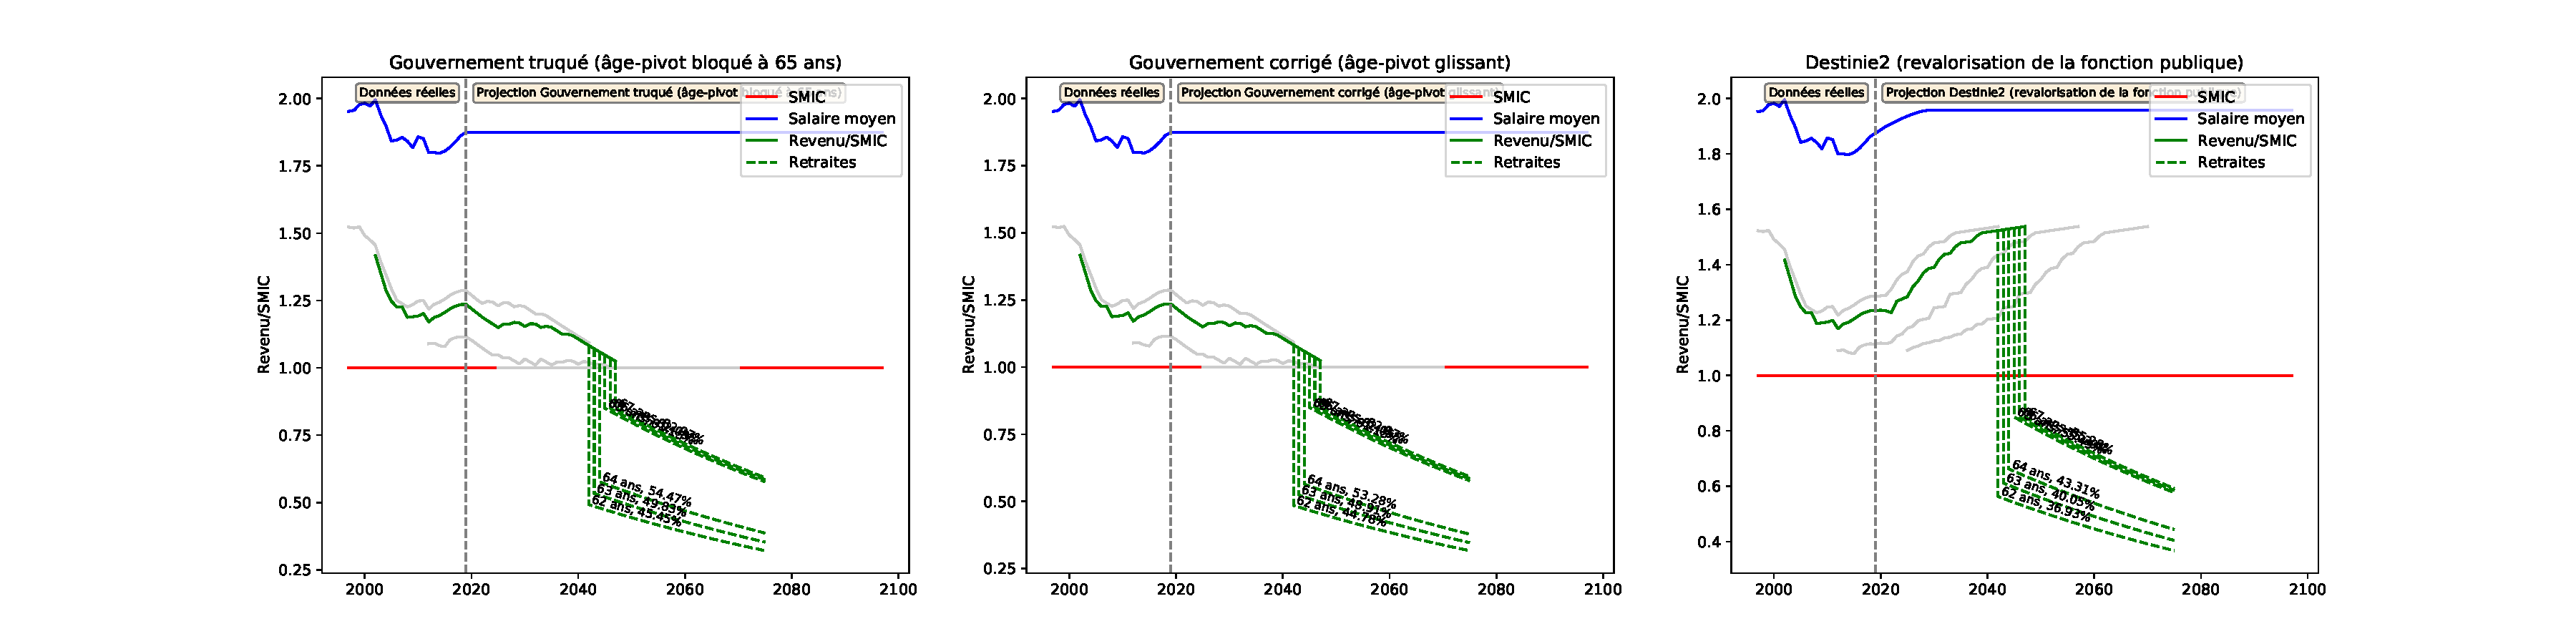
\includegraphics[width=0.9\textwidth]{fig/AideSoignant_1980_22_dest_retraite.pdf}\end{center} \label{fig/AideSoignant_1980_22_dest_retraite.pdf} 

\newpage 
 
\subsection{Génération 1990 (début en 2012)} 

\paragraph{Retraites possibles et ratios Revenu/SMIC à 70, 75, 80, 85, 90 ans avec le modèle \emph{Gouvernement truqué (âge-pivot bloqué à 65 ans)}}  
 
{ \scriptsize \begin{center} 
\begin{tabular}[htb]{|c|c||c|c||c|c||c||c|c|c|c|c|c|} 
\hline 
 Retraite en &  Âge &  Âge pivot &  Décote/Surcote &  Retraite (\euro{} 2019) &  Tx Rempl(\%) &  SMIC (\euro{} 2019) &  Retraite/SMIC &  Rev70/SMIC &  Rev75/SMIC &  Rev80/SMIC &  Rev85/SMIC &  Rev90/SMIC \\ 
\hline \hline 
 2052 &  62 &  65 ans 0 mois &  -15.00\% &  1199.24 &  {\bf 46.10} &  2601.14 &  {\bf {\color{red} 0.46}} &  {\bf {\color{red} 0.42}} &  {\bf {\color{red} 0.39}} &  {\bf {\color{red} 0.37}} &  {\bf {\color{red} 0.34}} &  {\bf {\color{red} 0.32}} \\ 
\hline 
 2053 &  63 &  65 ans 0 mois &  -10.00\% &  1319.30 &  {\bf 50.07} &  2634.96 &  {\bf {\color{red} 0.50}} &  {\bf {\color{red} 0.46}} &  {\bf {\color{red} 0.43}} &  {\bf {\color{red} 0.40}} &  {\bf {\color{red} 0.38}} &  {\bf {\color{red} 0.35}} \\ 
\hline 
 2054 &  64 &  65 ans 0 mois &  -5.00\% &  1445.99 &  {\bf 54.17} &  2669.21 &  {\bf {\color{red} 0.54}} &  {\bf {\color{red} 0.50}} &  {\bf {\color{red} 0.47}} &  {\bf {\color{red} 0.44}} &  {\bf {\color{red} 0.41}} &  {\bf {\color{red} 0.39}} \\ 
\hline 
 2055 &  65 &  65 ans 0 mois &  0.00\% &  2298.33 &  {\bf 85.00} &  2703.91 &  {\bf {\color{red} 0.85}} &  {\bf {\color{red} 0.80}} &  {\bf {\color{red} 0.75}} &  {\bf {\color{red} 0.70}} &  {\bf {\color{red} 0.66}} &  {\bf {\color{red} 0.62}} \\ 
\hline 
 2056 &  66 &  65 ans 0 mois &  5.00\% &  2328.20 &  {\bf 85.00} &  2739.06 &  {\bf {\color{red} 0.85}} &  {\bf {\color{red} 0.81}} &  {\bf {\color{red} 0.76}} &  {\bf {\color{red} 0.71}} &  {\bf {\color{red} 0.67}} &  {\bf {\color{red} 0.62}} \\ 
\hline 
 2057 &  67 &  65 ans 0 mois &  10.00\% &  2358.47 &  {\bf 85.00} &  2774.67 &  {\bf {\color{red} 0.85}} &  {\bf {\color{red} 0.82}} &  {\bf {\color{red} 0.77}} &  {\bf {\color{red} 0.72}} &  {\bf {\color{red} 0.67}} &  {\bf {\color{red} 0.63}} \\ 
\hline 
\hline 
\end{tabular} 
\end{center} } 
\paragraph{Retraites possibles et ratios Revenu/SMIC à 70, 75, 80, 85, 90 ans avec le modèle \emph{Gouvernement corrigé (âge-pivot glissant)}}  
 
{ \scriptsize \begin{center} 
\begin{tabular}[htb]{|c|c||c|c||c|c||c||c|c|c|c|c|c|} 
\hline 
 Retraite en &  Âge &  Âge pivot &  Décote/Surcote &  Retraite (\euro{} 2019) &  Tx Rempl(\%) &  SMIC (\euro{} 2019) &  Retraite/SMIC &  Rev70/SMIC &  Rev75/SMIC &  Rev80/SMIC &  Rev85/SMIC &  Rev90/SMIC \\ 
\hline \hline 
 2052 &  62 &  66 ans 1 mois &  -20.42\% &  1122.82 &  {\bf 43.17} &  2601.14 &  {\bf {\color{red} 0.43}} &  {\bf {\color{red} 0.39}} &  {\bf {\color{red} 0.36}} &  {\bf {\color{red} 0.34}} &  {\bf {\color{red} 0.32}} &  {\bf {\color{red} 0.30}} \\ 
\hline 
 2053 &  63 &  66 ans 2 mois &  -15.83\% &  1233.79 &  {\bf 46.82} &  2634.96 &  {\bf {\color{red} 0.47}} &  {\bf {\color{red} 0.43}} &  {\bf {\color{red} 0.40}} &  {\bf {\color{red} 0.38}} &  {\bf {\color{red} 0.35}} &  {\bf {\color{red} 0.33}} \\ 
\hline 
 2054 &  64 &  66 ans 3 mois &  -11.25\% &  1350.86 &  {\bf 50.61} &  2669.21 &  {\bf {\color{red} 0.51}} &  {\bf {\color{red} 0.47}} &  {\bf {\color{red} 0.44}} &  {\bf {\color{red} 0.41}} &  {\bf {\color{red} 0.39}} &  {\bf {\color{red} 0.36}} \\ 
\hline 
 2055 &  65 &  66 ans 4 mois &  -6.67\% &  2298.33 &  {\bf 85.00} &  2703.91 &  {\bf {\color{red} 0.85}} &  {\bf {\color{red} 0.80}} &  {\bf {\color{red} 0.75}} &  {\bf {\color{red} 0.70}} &  {\bf {\color{red} 0.66}} &  {\bf {\color{red} 0.62}} \\ 
\hline 
 2056 &  66 &  66 ans 5 mois &  -2.08\% &  2328.20 &  {\bf 85.00} &  2739.06 &  {\bf {\color{red} 0.85}} &  {\bf {\color{red} 0.81}} &  {\bf {\color{red} 0.76}} &  {\bf {\color{red} 0.71}} &  {\bf {\color{red} 0.67}} &  {\bf {\color{red} 0.62}} \\ 
\hline 
 2057 &  67 &  66 ans 6 mois &  2.50\% &  2358.47 &  {\bf 85.00} &  2774.67 &  {\bf {\color{red} 0.85}} &  {\bf {\color{red} 0.82}} &  {\bf {\color{red} 0.77}} &  {\bf {\color{red} 0.72}} &  {\bf {\color{red} 0.67}} &  {\bf {\color{red} 0.63}} \\ 
\hline 
\hline 
\end{tabular} 
\end{center} } 
\paragraph{Retraites possibles et ratios Revenu/SMIC à 70, 75, 80, 85, 90 ans avec le modèle \emph{Destinie2 (revalorisation de la fonction publique)}}  
 
{ \scriptsize \begin{center} 
\begin{tabular}[htb]{|c|c||c|c||c|c||c||c|c|c|c|c|c|} 
\hline 
 Retraite en &  Âge &  Âge pivot &  Décote/Surcote &  Retraite (\euro{} 2019) &  Tx Rempl(\%) &  SMIC (\euro{} 2019) &  Retraite/SMIC &  Rev70/SMIC &  Rev75/SMIC &  Rev80/SMIC &  Rev85/SMIC &  Rev90/SMIC \\ 
\hline \hline 
 2052 &  62 &  66 ans 1 mois &  -20.42\% &  1392.73 &  {\bf 37.18} &  2445.56 &  {\bf {\color{red} 0.57}} &  {\bf {\color{red} 0.51}} &  {\bf {\color{red} 0.48}} &  {\bf {\color{red} 0.45}} &  {\bf {\color{red} 0.42}} &  {\bf {\color{red} 0.40}} \\ 
\hline 
 2053 &  63 &  66 ans 2 mois &  -15.83\% &  1536.55 &  {\bf 40.49} &  2477.35 &  {\bf {\color{red} 0.62}} &  {\bf {\color{red} 0.57}} &  {\bf {\color{red} 0.53}} &  {\bf {\color{red} 0.50}} &  {\bf {\color{red} 0.47}} &  {\bf {\color{red} 0.44}} \\ 
\hline 
 2054 &  64 &  66 ans 3 mois &  -11.25\% &  1688.77 &  {\bf 43.93} &  2509.56 &  {\bf {\color{red} 0.67}} &  {\bf {\color{red} 0.62}} &  {\bf {\color{red} 0.58}} &  {\bf {\color{red} 0.55}} &  {\bf {\color{red} 0.51}} &  {\bf {\color{red} 0.48}} \\ 
\hline 
 2055 &  65 &  66 ans 4 mois &  -6.67\% &  2160.85 &  {\bf 55.49} &  2542.18 &  {\bf {\color{red} 0.85}} &  {\bf {\color{red} 0.80}} &  {\bf {\color{red} 0.75}} &  {\bf {\color{red} 0.70}} &  {\bf {\color{red} 0.66}} &  {\bf {\color{red} 0.62}} \\ 
\hline 
 2056 &  66 &  66 ans 5 mois &  -2.08\% &  2188.95 &  {\bf 55.49} &  2575.23 &  {\bf {\color{red} 0.85}} &  {\bf {\color{red} 0.81}} &  {\bf {\color{red} 0.76}} &  {\bf {\color{red} 0.71}} &  {\bf {\color{red} 0.67}} &  {\bf {\color{red} 0.62}} \\ 
\hline 
 2057 &  67 &  66 ans 6 mois &  2.50\% &  2217.40 &  {\bf 55.49} &  2608.71 &  {\bf {\color{red} 0.85}} &  {\bf {\color{red} 0.82}} &  {\bf {\color{red} 0.77}} &  {\bf {\color{red} 0.72}} &  {\bf {\color{red} 0.67}} &  {\bf {\color{red} 0.63}} \\ 
\hline 
\hline 
\end{tabular} 
\end{center} } 

 \begin{center}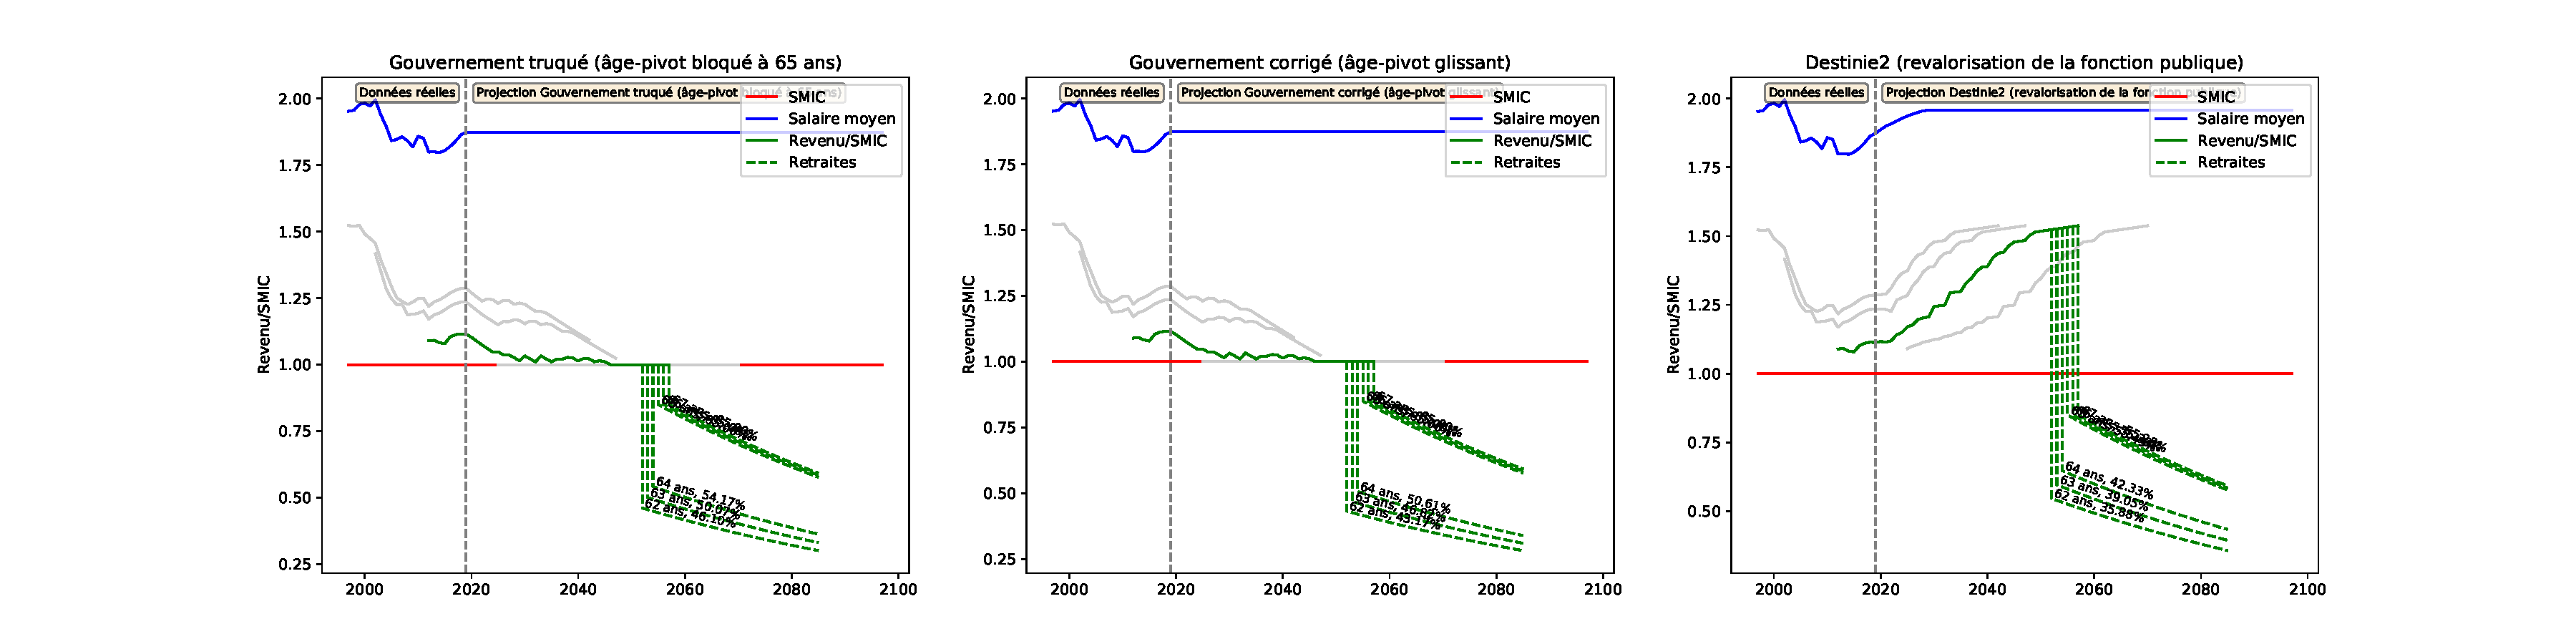
\includegraphics[width=0.9\textwidth]{fig/AideSoignant_1990_22_dest_retraite.pdf}\end{center} \label{fig/AideSoignant_1990_22_dest_retraite.pdf} 

\newpage 
 
\subsection{Génération 2003 (début en 2025)} 

\paragraph{Retraites possibles et ratios Revenu/SMIC à 70, 75, 80, 85, 90 ans avec le modèle \emph{Gouvernement truqué (âge-pivot bloqué à 65 ans)}}  
 
{ \scriptsize \begin{center} 
\begin{tabular}[htb]{|c|c||c|c||c|c||c||c|c|c|c|c|c|} 
\hline 
 Retraite en &  Âge &  Âge pivot &  Décote/Surcote &  Retraite (\euro{} 2019) &  Tx Rempl(\%) &  SMIC (\euro{} 2019) &  Retraite/SMIC &  Rev70/SMIC &  Rev75/SMIC &  Rev80/SMIC &  Rev85/SMIC &  Rev90/SMIC \\ 
\hline \hline 
 2065 &  62 &  65 ans 0 mois &  -15.00\% &  1457.41 &  {\bf 47.37} &  3076.71 &  {\bf {\color{red} 0.47}} &  {\bf {\color{red} 0.43}} &  {\bf {\color{red} 0.40}} &  {\bf {\color{red} 0.38}} &  {\bf {\color{red} 0.35}} &  {\bf {\color{red} 0.33}} \\ 
\hline 
 2066 &  63 &  65 ans 0 mois &  -10.00\% &  1602.25 &  {\bf 51.41} &  3116.71 &  {\bf {\color{red} 0.51}} &  {\bf {\color{red} 0.47}} &  {\bf {\color{red} 0.44}} &  {\bf {\color{red} 0.41}} &  {\bf {\color{red} 0.39}} &  {\bf {\color{red} 0.36}} \\ 
\hline 
 2067 &  64 &  65 ans 0 mois &  -5.00\% &  1755.00 &  {\bf 55.59} &  3157.23 &  {\bf {\color{red} 0.56}} &  {\bf {\color{red} 0.51}} &  {\bf {\color{red} 0.48}} &  {\bf {\color{red} 0.45}} &  {\bf {\color{red} 0.42}} &  {\bf {\color{red} 0.40}} \\ 
\hline 
 2068 &  65 &  65 ans 0 mois &  0.00\% &  2718.53 &  {\bf 85.00} &  3198.27 &  {\bf {\color{red} 0.85}} &  {\bf {\color{red} 0.80}} &  {\bf {\color{red} 0.75}} &  {\bf {\color{red} 0.70}} &  {\bf {\color{red} 0.66}} &  {\bf {\color{red} 0.62}} \\ 
\hline 
 2069 &  66 &  65 ans 0 mois &  5.00\% &  2753.87 &  {\bf 85.00} &  3239.85 &  {\bf {\color{red} 0.85}} &  {\bf {\color{red} 0.81}} &  {\bf {\color{red} 0.76}} &  {\bf {\color{red} 0.71}} &  {\bf {\color{red} 0.67}} &  {\bf {\color{red} 0.62}} \\ 
\hline 
 2070 &  67 &  65 ans 0 mois &  10.00\% &  2789.67 &  {\bf 85.00} &  3281.97 &  {\bf {\color{red} 0.85}} &  {\bf {\color{red} 0.82}} &  {\bf {\color{red} 0.77}} &  {\bf {\color{red} 0.72}} &  {\bf {\color{red} 0.67}} &  {\bf {\color{red} 0.63}} \\ 
\hline 
\hline 
\end{tabular} 
\end{center} } 
\paragraph{Retraites possibles et ratios Revenu/SMIC à 70, 75, 80, 85, 90 ans avec le modèle \emph{Gouvernement corrigé (âge-pivot glissant)}}  
 
{ \scriptsize \begin{center} 
\begin{tabular}[htb]{|c|c||c|c||c|c||c||c|c|c|c|c|c|} 
\hline 
 Retraite en &  Âge &  Âge pivot &  Décote/Surcote &  Retraite (\euro{} 2019) &  Tx Rempl(\%) &  SMIC (\euro{} 2019) &  Retraite/SMIC &  Rev70/SMIC &  Rev75/SMIC &  Rev80/SMIC &  Rev85/SMIC &  Rev90/SMIC \\ 
\hline \hline 
 2065 &  62 &  67 ans 2 mois &  -25.83\% &  1271.67 &  {\bf 41.33} &  3076.71 &  {\bf {\color{red} 0.41}} &  {\bf {\color{red} 0.37}} &  {\bf {\color{red} 0.35}} &  {\bf {\color{red} 0.33}} &  {\bf {\color{red} 0.31}} &  {\bf {\color{red} 0.29}} \\ 
\hline 
 2066 &  63 &  67 ans 3 mois &  -21.25\% &  1401.97 &  {\bf 44.98} &  3116.71 &  {\bf {\color{red} 0.45}} &  {\bf {\color{red} 0.41}} &  {\bf {\color{red} 0.39}} &  {\bf {\color{red} 0.36}} &  {\bf {\color{red} 0.34}} &  {\bf {\color{red} 0.32}} \\ 
\hline 
 2067 &  64 &  67 ans 4 mois &  -16.67\% &  1539.47 &  {\bf 48.76} &  3157.23 &  {\bf {\color{red} 0.49}} &  {\bf {\color{red} 0.45}} &  {\bf {\color{red} 0.42}} &  {\bf {\color{red} 0.40}} &  {\bf {\color{red} 0.37}} &  {\bf {\color{red} 0.35}} \\ 
\hline 
 2068 &  65 &  67 ans 5 mois &  -12.08\% &  2718.53 &  {\bf 85.00} &  3198.27 &  {\bf {\color{red} 0.85}} &  {\bf {\color{red} 0.80}} &  {\bf {\color{red} 0.75}} &  {\bf {\color{red} 0.70}} &  {\bf {\color{red} 0.66}} &  {\bf {\color{red} 0.62}} \\ 
\hline 
 2069 &  66 &  67 ans 6 mois &  -7.50\% &  2753.87 &  {\bf 85.00} &  3239.85 &  {\bf {\color{red} 0.85}} &  {\bf {\color{red} 0.81}} &  {\bf {\color{red} 0.76}} &  {\bf {\color{red} 0.71}} &  {\bf {\color{red} 0.67}} &  {\bf {\color{red} 0.62}} \\ 
\hline 
 2070 &  67 &  67 ans 7 mois &  -2.92\% &  2789.67 &  {\bf 85.00} &  3281.97 &  {\bf {\color{red} 0.85}} &  {\bf {\color{red} 0.82}} &  {\bf {\color{red} 0.77}} &  {\bf {\color{red} 0.72}} &  {\bf {\color{red} 0.67}} &  {\bf {\color{red} 0.63}} \\ 
\hline 
\hline 
\end{tabular} 
\end{center} } 
\paragraph{Retraites possibles et ratios Revenu/SMIC à 70, 75, 80, 85, 90 ans avec le modèle \emph{Destinie2 (revalorisation de la fonction publique)}}  
 
{ \scriptsize \begin{center} 
\begin{tabular}[htb]{|c|c||c|c||c|c||c||c|c|c|c|c|c|} 
\hline 
 Retraite en &  Âge &  Âge pivot &  Décote/Surcote &  Retraite (\euro{} 2019) &  Tx Rempl(\%) &  SMIC (\euro{} 2019) &  Retraite/SMIC &  Rev70/SMIC &  Rev75/SMIC &  Rev80/SMIC &  Rev85/SMIC &  Rev90/SMIC \\ 
\hline \hline 
 2065 &  62 &  67 ans 2 mois &  -25.83\% &  1613.13 &  {\bf 36.40} &  2892.68 &  {\bf {\color{red} 0.56}} &  {\bf {\color{red} 0.50}} &  {\bf {\color{red} 0.47}} &  {\bf {\color{red} 0.44}} &  {\bf {\color{red} 0.41}} &  {\bf {\color{red} 0.39}} \\ 
\hline 
 2066 &  63 &  67 ans 3 mois &  -21.25\% &  1784.29 &  {\bf 39.75} &  2930.29 &  {\bf {\color{red} 0.61}} &  {\bf {\color{red} 0.56}} &  {\bf {\color{red} 0.52}} &  {\bf {\color{red} 0.49}} &  {\bf {\color{red} 0.46}} &  {\bf {\color{red} 0.43}} \\ 
\hline 
 2067 &  64 &  67 ans 4 mois &  -16.67\% &  1965.43 &  {\bf 43.22} &  2968.38 &  {\bf {\color{red} 0.66}} &  {\bf {\color{red} 0.61}} &  {\bf {\color{red} 0.57}} &  {\bf {\color{red} 0.54}} &  {\bf {\color{red} 0.50}} &  {\bf {\color{red} 0.47}} \\ 
\hline 
 2068 &  65 &  67 ans 5 mois &  -12.08\% &  2555.93 &  {\bf 55.49} &  3006.97 &  {\bf {\color{red} 0.85}} &  {\bf {\color{red} 0.80}} &  {\bf {\color{red} 0.75}} &  {\bf {\color{red} 0.70}} &  {\bf {\color{red} 0.66}} &  {\bf {\color{red} 0.62}} \\ 
\hline 
 2069 &  66 &  67 ans 6 mois &  -7.50\% &  2589.15 &  {\bf 55.49} &  3046.06 &  {\bf {\color{red} 0.85}} &  {\bf {\color{red} 0.81}} &  {\bf {\color{red} 0.76}} &  {\bf {\color{red} 0.71}} &  {\bf {\color{red} 0.67}} &  {\bf {\color{red} 0.62}} \\ 
\hline 
 2070 &  67 &  67 ans 7 mois &  -2.92\% &  2622.81 &  {\bf 55.49} &  3085.66 &  {\bf {\color{red} 0.85}} &  {\bf {\color{red} 0.82}} &  {\bf {\color{red} 0.77}} &  {\bf {\color{red} 0.72}} &  {\bf {\color{red} 0.67}} &  {\bf {\color{red} 0.63}} \\ 
\hline 
\hline 
\end{tabular} 
\end{center} } 

 \begin{center}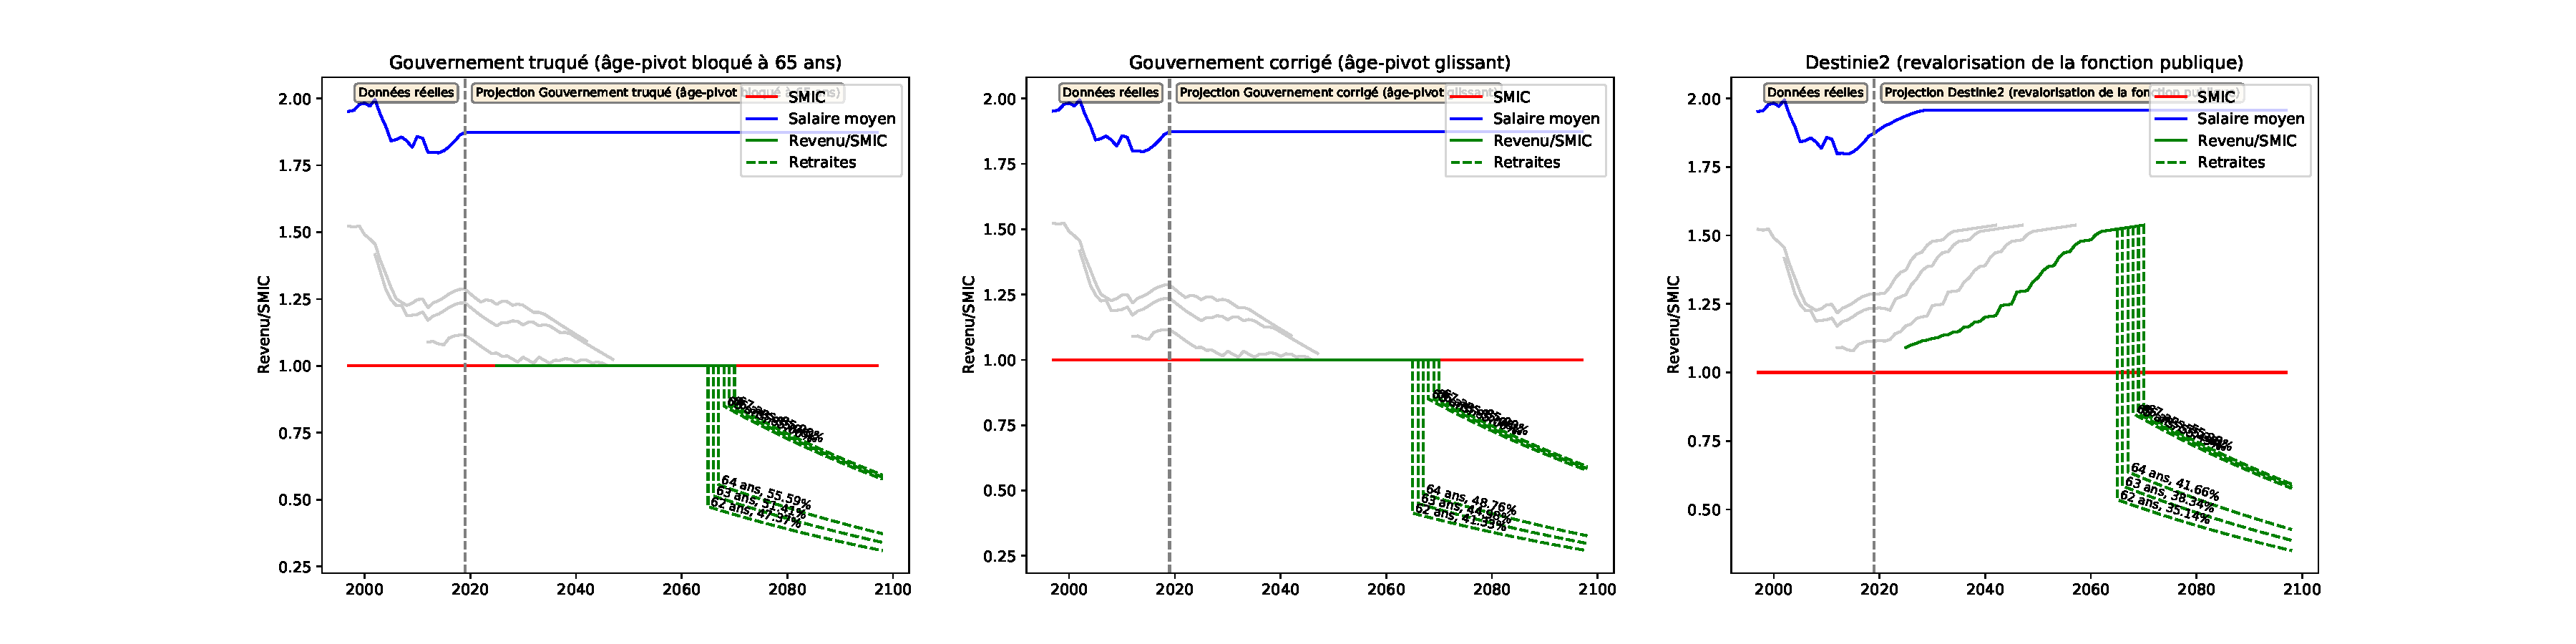
\includegraphics[width=0.9\textwidth]{fig/AideSoignant_2003_22_dest_retraite.pdf}\end{center} \label{fig/AideSoignant_2003_22_dest_retraite.pdf} 

\newpage 
 
\chapter{Technicien hospitalier} 

\begin{minipage}{0.55\linewidth}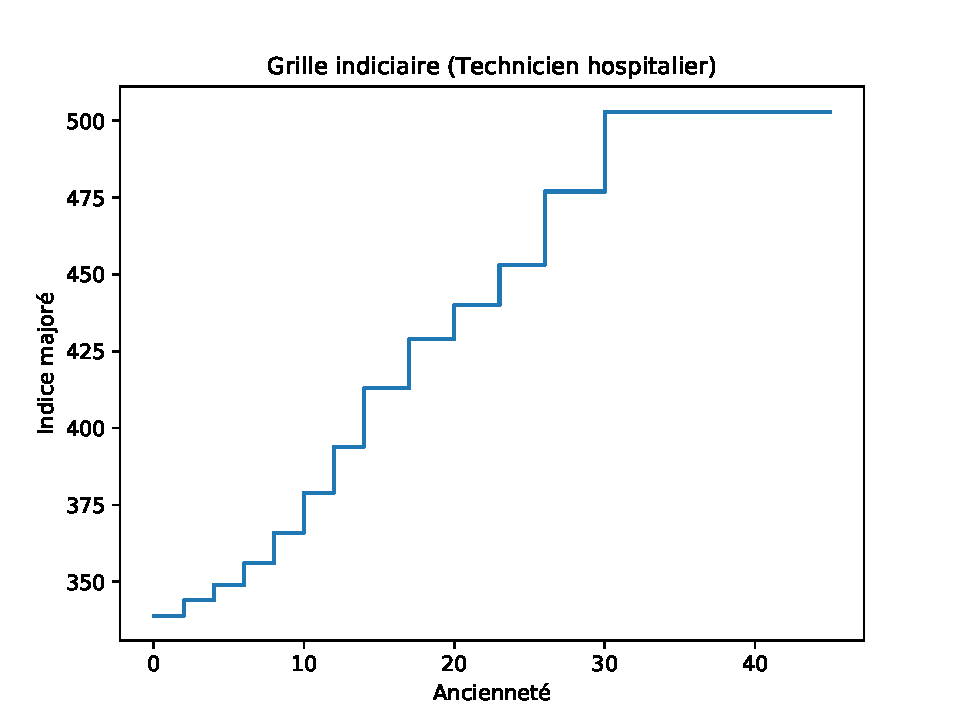
\includegraphics[width=0.7\textwidth]{fig/grille_TechHosp.pdf}\end{minipage} 
\begin{minipage}{0.3\linewidth} 
 \begin{center} 

\begin{tabular}[htb]{|c|c|} 
\hline 
 Indice majoré &  Durée (années) \\ 
\hline \hline 
 339 &  2.00 \\ 
\hline 
 344 &  2.00 \\ 
\hline 
 349 &  2.00 \\ 
\hline 
 356 &  2.00 \\ 
\hline 
 366 &  2.00 \\ 
\hline 
 379 &  2.00 \\ 
\hline 
 394 &  2.00 \\ 
\hline 
 413 &  3.00 \\ 
\hline 
 429 &  3.00 \\ 
\hline 
 440 &  3.00 \\ 
\hline 
 453 &  3.00 \\ 
\hline 
 477 &  4.00 \\ 
\hline 
 503 &   \\ 
\hline 
\hline 
\end{tabular} 
\end{center} 
 \end{minipage} 


 \addto{\captionsenglish}{ \renewcommand{\mtctitle}{}} \setcounter{minitocdepth}{2} 
 \minitoc \newpage 

\section{Début de carrière à 22 ans} 

\subsection{Génération 1975 (début en 1997)} 

\paragraph{Retraites possibles et ratios Revenu/SMIC à 70, 75, 80, 85, 90 ans avec le modèle \emph{Gouvernement truqué (âge-pivot bloqué à 65 ans)}}  
 
{ \scriptsize \begin{center} 
\begin{tabular}[htb]{|c|c||c|c||c|c||c||c|c|c|c|c|c|} 
\hline 
 Retraite en &  Âge &  Âge pivot &  Décote/Surcote &  Retraite (\euro{} 2019) &  Tx Rempl(\%) &  SMIC (\euro{} 2019) &  Retraite/SMIC &  Rev70/SMIC &  Rev75/SMIC &  Rev80/SMIC &  Rev85/SMIC &  Rev90/SMIC \\ 
\hline \hline 
 2037 &  62 &  64 ans 10 mois &  -14.17\% &  1321.60 &  {\bf 43.39} &  2143.00 &  {\bf {\color{red} 0.62}} &  {\bf {\color{red} 0.56}} &  {\bf {\color{red} 0.52}} &  {\bf {\color{red} 0.49}} &  {\bf {\color{red} 0.46}} &  {\bf {\color{red} 0.43}} \\ 
\hline 
 2038 &  63 &  64 ans 11 mois &  -9.58\% &  1441.19 &  {\bf 47.23} &  2170.86 &  {\bf {\color{red} 0.66}} &  {\bf {\color{red} 0.61}} &  {\bf {\color{red} 0.57}} &  {\bf {\color{red} 0.53}} &  {\bf {\color{red} 0.50}} &  {\bf {\color{red} 0.47}} \\ 
\hline 
 2039 &  64 &  65 ans 0 mois &  -5.00\% &  1567.38 &  {\bf 51.27} &  2199.08 &  {\bf {\color{red} 0.71}} &  {\bf {\color{red} 0.66}} &  {\bf {\color{red} 0.62}} &  {\bf {\color{red} 0.58}} &  {\bf {\color{red} 0.54}} &  {\bf {\color{red} 0.51}} \\ 
\hline 
 2040 &  65 &  65 ans 0 mois &  0.00\% &  1893.52 &  {\bf 61.82} &  2227.67 &  {\bf {\color{red} 0.85}} &  {\bf {\color{red} 0.80}} &  {\bf {\color{red} 0.75}} &  {\bf {\color{red} 0.70}} &  {\bf {\color{red} 0.66}} &  {\bf {\color{red} 0.62}} \\ 
\hline 
 2041 &  66 &  65 ans 0 mois &  5.00\% &  1918.14 &  {\bf 62.52} &  2256.63 &  {\bf {\color{red} 0.85}} &  {\bf {\color{red} 0.81}} &  {\bf {\color{red} 0.76}} &  {\bf {\color{red} 0.71}} &  {\bf {\color{red} 0.67}} &  {\bf {\color{red} 0.62}} \\ 
\hline 
 2042 &  67 &  65 ans 0 mois &  10.00\% &  2011.85 &  {\bf 65.45} &  2285.97 &  {\bf {\color{red} 0.88}} &  {\bf {\color{red} 0.85}} &  {\bf {\color{red} 0.79}} &  {\bf {\color{red} 0.74}} &  {\bf {\color{red} 0.70}} &  {\bf {\color{red} 0.65}} \\ 
\hline 
\hline 
\end{tabular} 
\end{center} } 
\paragraph{Retraites possibles et ratios Revenu/SMIC à 70, 75, 80, 85, 90 ans avec le modèle \emph{Gouvernement corrigé (âge-pivot glissant)}}  
 
{ \scriptsize \begin{center} 
\begin{tabular}[htb]{|c|c||c|c||c|c||c||c|c|c|c|c|c|} 
\hline 
 Retraite en &  Âge &  Âge pivot &  Décote/Surcote &  Retraite (\euro{} 2019) &  Tx Rempl(\%) &  SMIC (\euro{} 2019) &  Retraite/SMIC &  Rev70/SMIC &  Rev75/SMIC &  Rev80/SMIC &  Rev85/SMIC &  Rev90/SMIC \\ 
\hline \hline 
 2037 &  62 &  64 ans 10 mois &  -14.17\% &  1321.60 &  {\bf 43.39} &  2143.00 &  {\bf {\color{red} 0.62}} &  {\bf {\color{red} 0.56}} &  {\bf {\color{red} 0.52}} &  {\bf {\color{red} 0.49}} &  {\bf {\color{red} 0.46}} &  {\bf {\color{red} 0.43}} \\ 
\hline 
 2038 &  63 &  64 ans 11 mois &  -9.58\% &  1441.19 &  {\bf 47.23} &  2170.86 &  {\bf {\color{red} 0.66}} &  {\bf {\color{red} 0.61}} &  {\bf {\color{red} 0.57}} &  {\bf {\color{red} 0.53}} &  {\bf {\color{red} 0.50}} &  {\bf {\color{red} 0.47}} \\ 
\hline 
 2039 &  64 &  65 ans 0 mois &  -5.00\% &  1567.38 &  {\bf 51.27} &  2199.08 &  {\bf {\color{red} 0.71}} &  {\bf {\color{red} 0.66}} &  {\bf {\color{red} 0.62}} &  {\bf {\color{red} 0.58}} &  {\bf {\color{red} 0.54}} &  {\bf {\color{red} 0.51}} \\ 
\hline 
 2040 &  65 &  65 ans 1 mois &  -0.42\% &  1893.52 &  {\bf 61.82} &  2227.67 &  {\bf {\color{red} 0.85}} &  {\bf {\color{red} 0.80}} &  {\bf {\color{red} 0.75}} &  {\bf {\color{red} 0.70}} &  {\bf {\color{red} 0.66}} &  {\bf {\color{red} 0.62}} \\ 
\hline 
 2041 &  66 &  65 ans 2 mois &  4.17\% &  1918.14 &  {\bf 62.52} &  2256.63 &  {\bf {\color{red} 0.85}} &  {\bf {\color{red} 0.81}} &  {\bf {\color{red} 0.76}} &  {\bf {\color{red} 0.71}} &  {\bf {\color{red} 0.67}} &  {\bf {\color{red} 0.62}} \\ 
\hline 
 2042 &  67 &  65 ans 3 mois &  8.75\% &  1988.99 &  {\bf 64.71} &  2285.97 &  {\bf {\color{red} 0.87}} &  {\bf {\color{red} 0.84}} &  {\bf {\color{red} 0.78}} &  {\bf {\color{red} 0.74}} &  {\bf {\color{red} 0.69}} &  {\bf {\color{red} 0.65}} \\ 
\hline 
\hline 
\end{tabular} 
\end{center} } 
\paragraph{Retraites possibles et ratios Revenu/SMIC à 70, 75, 80, 85, 90 ans avec le modèle \emph{Destinie2 (revalorisation de la fonction publique)}}  
 
{ \scriptsize \begin{center} 
\begin{tabular}[htb]{|c|c||c|c||c|c||c||c|c|c|c|c|c|} 
\hline 
 Retraite en &  Âge &  Âge pivot &  Décote/Surcote &  Retraite (\euro{} 2019) &  Tx Rempl(\%) &  SMIC (\euro{} 2019) &  Retraite/SMIC &  Rev70/SMIC &  Rev75/SMIC &  Rev80/SMIC &  Rev85/SMIC &  Rev90/SMIC \\ 
\hline \hline 
 2037 &  62 &  64 ans 10 mois &  -14.17\% &  1455.57 &  {\bf 38.33} &  2014.82 &  {\bf {\color{red} 0.72}} &  {\bf {\color{red} 0.65}} &  {\bf {\color{red} 0.61}} &  {\bf {\color{red} 0.57}} &  {\bf {\color{red} 0.54}} &  {\bf {\color{red} 0.50}} \\ 
\hline 
 2038 &  63 &  64 ans 11 mois &  -9.58\% &  1593.40 &  {\bf 41.42} &  2041.01 &  {\bf {\color{red} 0.78}} &  {\bf {\color{red} 0.71}} &  {\bf {\color{red} 0.67}} &  {\bf {\color{red} 0.63}} &  {\bf {\color{red} 0.59}} &  {\bf {\color{red} 0.55}} \\ 
\hline 
 2039 &  64 &  65 ans 0 mois &  -5.00\% &  1739.76 &  {\bf 44.64} &  2067.55 &  {\bf {\color{red} 0.84}} &  {\bf {\color{red} 0.78}} &  {\bf {\color{red} 0.73}} &  {\bf {\color{red} 0.68}} &  {\bf {\color{red} 0.64}} &  {\bf {\color{red} 0.60}} \\ 
\hline 
 2040 &  65 &  65 ans 1 mois &  -0.42\% &  1895.12 &  {\bf 48.01} &  2094.43 &  {\bf {\color{red} 0.90}} &  {\bf {\color{red} 0.85}} &  {\bf {\color{red} 0.80}} &  {\bf {\color{red} 0.75}} &  {\bf {\color{red} 0.70}} &  {\bf {\color{red} 0.66}} \\ 
\hline 
 2041 &  66 &  65 ans 2 mois &  4.17\% &  2060.00 &  {\bf 51.51} &  2121.65 &  {\bf {\color{red} 0.97}} &  {\bf {\color{red} 0.92}} &  {\bf {\color{red} 0.86}} &  {\bf {\color{red} 0.81}} &  {\bf {\color{red} 0.76}} &  {\bf {\color{red} 0.71}} \\ 
\hline 
 2042 &  67 &  65 ans 3 mois &  8.75\% &  2234.96 &  {\bf 55.17} &  2149.23 &  {\bf 1.04} &  {\bf 1.00} &  {\bf {\color{red} 0.94}} &  {\bf {\color{red} 0.88}} &  {\bf {\color{red} 0.82}} &  {\bf {\color{red} 0.77}} \\ 
\hline 
\hline 
\end{tabular} 
\end{center} } 

 \begin{center}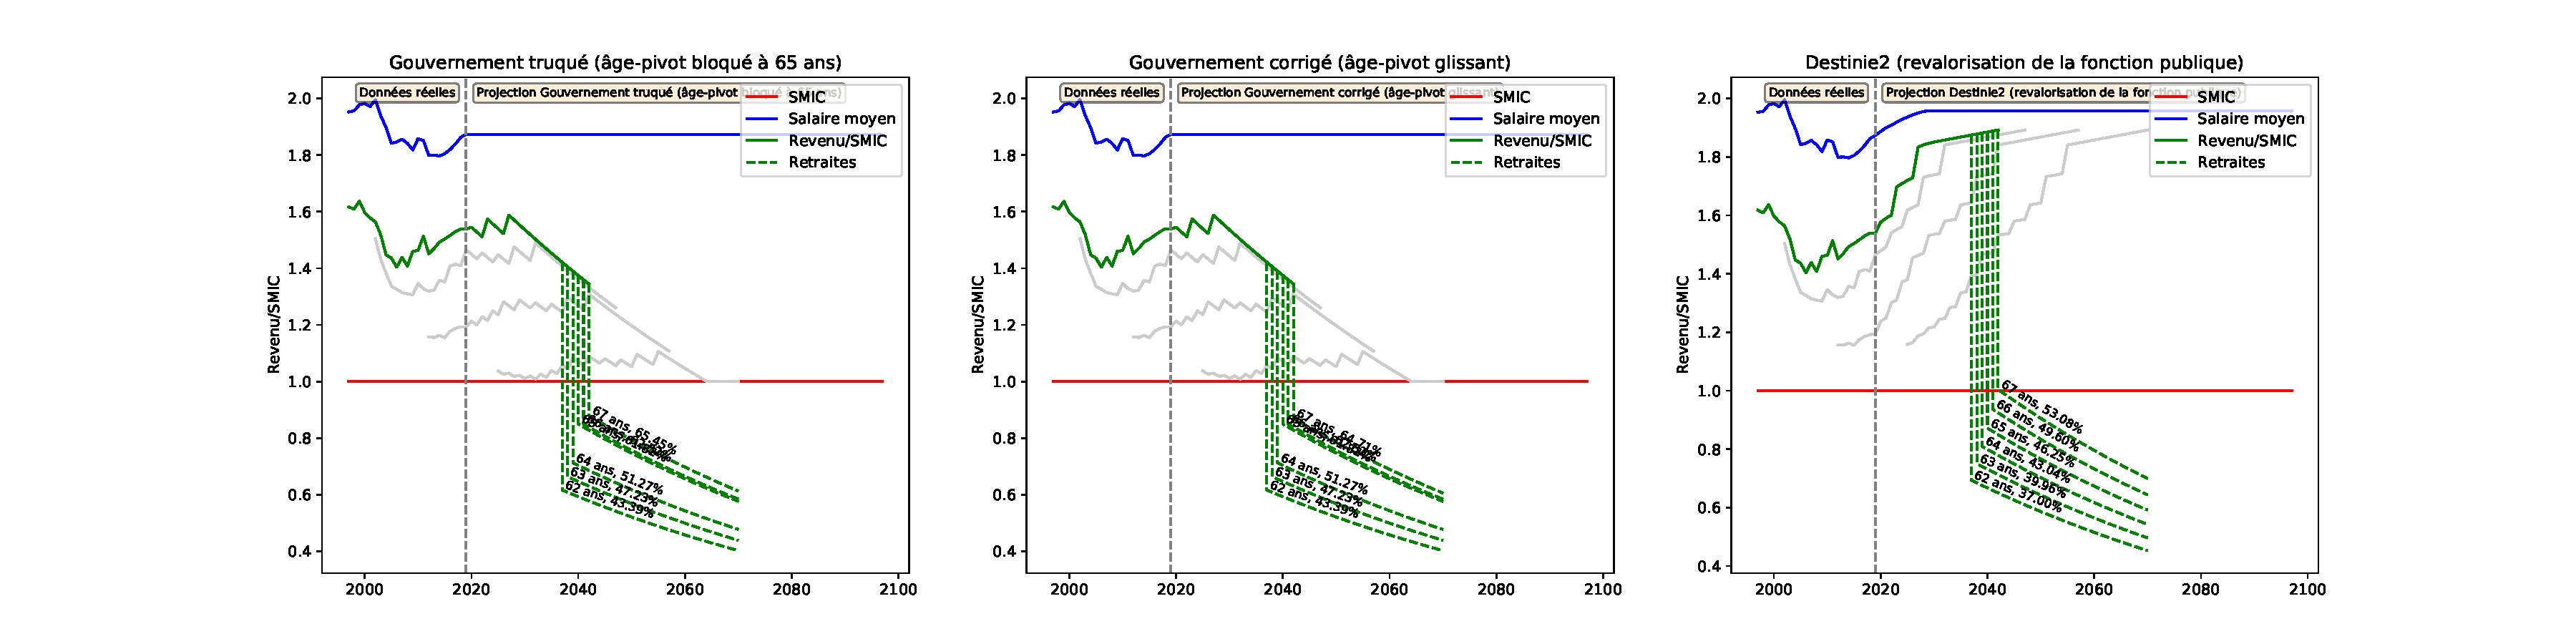
\includegraphics[width=0.9\textwidth]{fig/TechHosp_1975_22_dest_retraite.pdf}\end{center} \label{fig/TechHosp_1975_22_dest_retraite.pdf} 

\newpage 
 
\subsection{Génération 1980 (début en 2002)} 

\paragraph{Retraites possibles et ratios Revenu/SMIC à 70, 75, 80, 85, 90 ans avec le modèle \emph{Gouvernement truqué (âge-pivot bloqué à 65 ans)}}  
 
{ \scriptsize \begin{center} 
\begin{tabular}[htb]{|c|c||c|c||c|c||c||c|c|c|c|c|c|} 
\hline 
 Retraite en &  Âge &  Âge pivot &  Décote/Surcote &  Retraite (\euro{} 2019) &  Tx Rempl(\%) &  SMIC (\euro{} 2019) &  Retraite/SMIC &  Rev70/SMIC &  Rev75/SMIC &  Rev80/SMIC &  Rev85/SMIC &  Rev90/SMIC \\ 
\hline \hline 
 2042 &  62 &  65 ans 0 mois &  -15.00\% &  1334.51 &  {\bf 43.81} &  2285.97 &  {\bf {\color{red} 0.58}} &  {\bf {\color{red} 0.53}} &  {\bf {\color{red} 0.49}} &  {\bf {\color{red} 0.46}} &  {\bf {\color{red} 0.43}} &  {\bf {\color{red} 0.41}} \\ 
\hline 
 2043 &  63 &  65 ans 0 mois &  -10.00\% &  1467.43 &  {\bf 48.09} &  2315.68 &  {\bf {\color{red} 0.63}} &  {\bf {\color{red} 0.58}} &  {\bf {\color{red} 0.54}} &  {\bf {\color{red} 0.51}} &  {\bf {\color{red} 0.48}} &  {\bf {\color{red} 0.45}} \\ 
\hline 
 2044 &  64 &  65 ans 0 mois &  -5.00\% &  1608.33 &  {\bf 52.61} &  2345.79 &  {\bf {\color{red} 0.69}} &  {\bf {\color{red} 0.63}} &  {\bf {\color{red} 0.59}} &  {\bf {\color{red} 0.56}} &  {\bf {\color{red} 0.52}} &  {\bf {\color{red} 0.49}} \\ 
\hline 
 2045 &  65 &  65 ans 0 mois &  0.00\% &  2019.84 &  {\bf 65.95} &  2376.28 &  {\bf {\color{red} 0.85}} &  {\bf {\color{red} 0.80}} &  {\bf {\color{red} 0.75}} &  {\bf {\color{red} 0.70}} &  {\bf {\color{red} 0.66}} &  {\bf {\color{red} 0.62}} \\ 
\hline 
 2046 &  66 &  65 ans 0 mois &  5.00\% &  2046.10 &  {\bf 66.69} &  2407.18 &  {\bf {\color{red} 0.85}} &  {\bf {\color{red} 0.81}} &  {\bf {\color{red} 0.76}} &  {\bf {\color{red} 0.71}} &  {\bf {\color{red} 0.67}} &  {\bf {\color{red} 0.62}} \\ 
\hline 
 2047 &  67 &  65 ans 0 mois &  10.00\% &  2078.62 &  {\bf 67.62} &  2438.47 &  {\bf {\color{red} 0.85}} &  {\bf {\color{red} 0.82}} &  {\bf {\color{red} 0.77}} &  {\bf {\color{red} 0.72}} &  {\bf {\color{red} 0.68}} &  {\bf {\color{red} 0.63}} \\ 
\hline 
\hline 
\end{tabular} 
\end{center} } 
\paragraph{Retraites possibles et ratios Revenu/SMIC à 70, 75, 80, 85, 90 ans avec le modèle \emph{Gouvernement corrigé (âge-pivot glissant)}}  
 
{ \scriptsize \begin{center} 
\begin{tabular}[htb]{|c|c||c|c||c|c||c||c|c|c|c|c|c|} 
\hline 
 Retraite en &  Âge &  Âge pivot &  Décote/Surcote &  Retraite (\euro{} 2019) &  Tx Rempl(\%) &  SMIC (\euro{} 2019) &  Retraite/SMIC &  Rev70/SMIC &  Rev75/SMIC &  Rev80/SMIC &  Rev85/SMIC &  Rev90/SMIC \\ 
\hline \hline 
 2042 &  62 &  65 ans 3 mois &  -16.25\% &  1314.88 &  {\bf 43.17} &  2285.97 &  {\bf {\color{red} 0.58}} &  {\bf {\color{red} 0.52}} &  {\bf {\color{red} 0.49}} &  {\bf {\color{red} 0.46}} &  {\bf {\color{red} 0.43}} &  {\bf {\color{red} 0.40}} \\ 
\hline 
 2043 &  63 &  65 ans 4 mois &  -11.67\% &  1440.26 &  {\bf 47.20} &  2315.68 &  {\bf {\color{red} 0.62}} &  {\bf {\color{red} 0.57}} &  {\bf {\color{red} 0.53}} &  {\bf {\color{red} 0.50}} &  {\bf {\color{red} 0.47}} &  {\bf {\color{red} 0.44}} \\ 
\hline 
 2044 &  64 &  65 ans 5 mois &  -7.08\% &  1573.06 &  {\bf 51.45} &  2345.79 &  {\bf {\color{red} 0.67}} &  {\bf {\color{red} 0.62}} &  {\bf {\color{red} 0.58}} &  {\bf {\color{red} 0.55}} &  {\bf {\color{red} 0.51}} &  {\bf {\color{red} 0.48}} \\ 
\hline 
 2045 &  65 &  65 ans 6 mois &  -2.50\% &  2019.84 &  {\bf 65.95} &  2376.28 &  {\bf {\color{red} 0.85}} &  {\bf {\color{red} 0.80}} &  {\bf {\color{red} 0.75}} &  {\bf {\color{red} 0.70}} &  {\bf {\color{red} 0.66}} &  {\bf {\color{red} 0.62}} \\ 
\hline 
 2046 &  66 &  65 ans 7 mois &  2.08\% &  2046.10 &  {\bf 66.69} &  2407.18 &  {\bf {\color{red} 0.85}} &  {\bf {\color{red} 0.81}} &  {\bf {\color{red} 0.76}} &  {\bf {\color{red} 0.71}} &  {\bf {\color{red} 0.67}} &  {\bf {\color{red} 0.62}} \\ 
\hline 
 2047 &  67 &  65 ans 8 mois &  6.67\% &  2072.70 &  {\bf 67.43} &  2438.47 &  {\bf {\color{red} 0.85}} &  {\bf {\color{red} 0.82}} &  {\bf {\color{red} 0.77}} &  {\bf {\color{red} 0.72}} &  {\bf {\color{red} 0.67}} &  {\bf {\color{red} 0.63}} \\ 
\hline 
\hline 
\end{tabular} 
\end{center} } 
\paragraph{Retraites possibles et ratios Revenu/SMIC à 70, 75, 80, 85, 90 ans avec le modèle \emph{Destinie2 (revalorisation de la fonction publique)}}  
 
{ \scriptsize \begin{center} 
\begin{tabular}[htb]{|c|c||c|c||c|c||c||c|c|c|c|c|c|} 
\hline 
 Retraite en &  Âge &  Âge pivot &  Décote/Surcote &  Retraite (\euro{} 2019) &  Tx Rempl(\%) &  SMIC (\euro{} 2019) &  Retraite/SMIC &  Rev70/SMIC &  Rev75/SMIC &  Rev80/SMIC &  Rev85/SMIC &  Rev90/SMIC \\ 
\hline \hline 
 2042 &  62 &  65 ans 3 mois &  -16.25\% &  1499.43 &  {\bf 37.01} &  2149.23 &  {\bf {\color{red} 0.70}} &  {\bf {\color{red} 0.63}} &  {\bf {\color{red} 0.59}} &  {\bf {\color{red} 0.55}} &  {\bf {\color{red} 0.52}} &  {\bf {\color{red} 0.49}} \\ 
\hline 
 2043 &  63 &  65 ans 4 mois &  -11.67\% &  1650.07 &  {\bf 40.21} &  2177.17 &  {\bf {\color{red} 0.76}} &  {\bf {\color{red} 0.69}} &  {\bf {\color{red} 0.65}} &  {\bf {\color{red} 0.61}} &  {\bf {\color{red} 0.57}} &  {\bf {\color{red} 0.53}} \\ 
\hline 
 2044 &  64 &  65 ans 5 mois &  -7.08\% &  1810.68 &  {\bf 43.56} &  2205.48 &  {\bf {\color{red} 0.82}} &  {\bf {\color{red} 0.76}} &  {\bf {\color{red} 0.71}} &  {\bf {\color{red} 0.67}} &  {\bf {\color{red} 0.63}} &  {\bf {\color{red} 0.59}} \\ 
\hline 
 2045 &  65 &  65 ans 6 mois &  -2.50\% &  1981.85 &  {\bf 47.06} &  2234.15 &  {\bf {\color{red} 0.89}} &  {\bf {\color{red} 0.83}} &  {\bf {\color{red} 0.78}} &  {\bf {\color{red} 0.73}} &  {\bf {\color{red} 0.69}} &  {\bf {\color{red} 0.64}} \\ 
\hline 
 2046 &  66 &  65 ans 7 mois &  2.08\% &  2162.60 &  {\bf 50.70} &  2263.19 &  {\bf {\color{red} 0.96}} &  {\bf {\color{red} 0.91}} &  {\bf {\color{red} 0.85}} &  {\bf {\color{red} 0.80}} &  {\bf {\color{red} 0.75}} &  {\bf {\color{red} 0.70}} \\ 
\hline 
 2047 &  67 &  65 ans 8 mois &  6.67\% &  2353.23 &  {\bf 54.46} &  2292.61 &  {\bf 1.03} &  {\bf {\color{red} 0.99}} &  {\bf {\color{red} 0.93}} &  {\bf {\color{red} 0.87}} &  {\bf {\color{red} 0.81}} &  {\bf {\color{red} 0.76}} \\ 
\hline 
\hline 
\end{tabular} 
\end{center} } 

 \begin{center}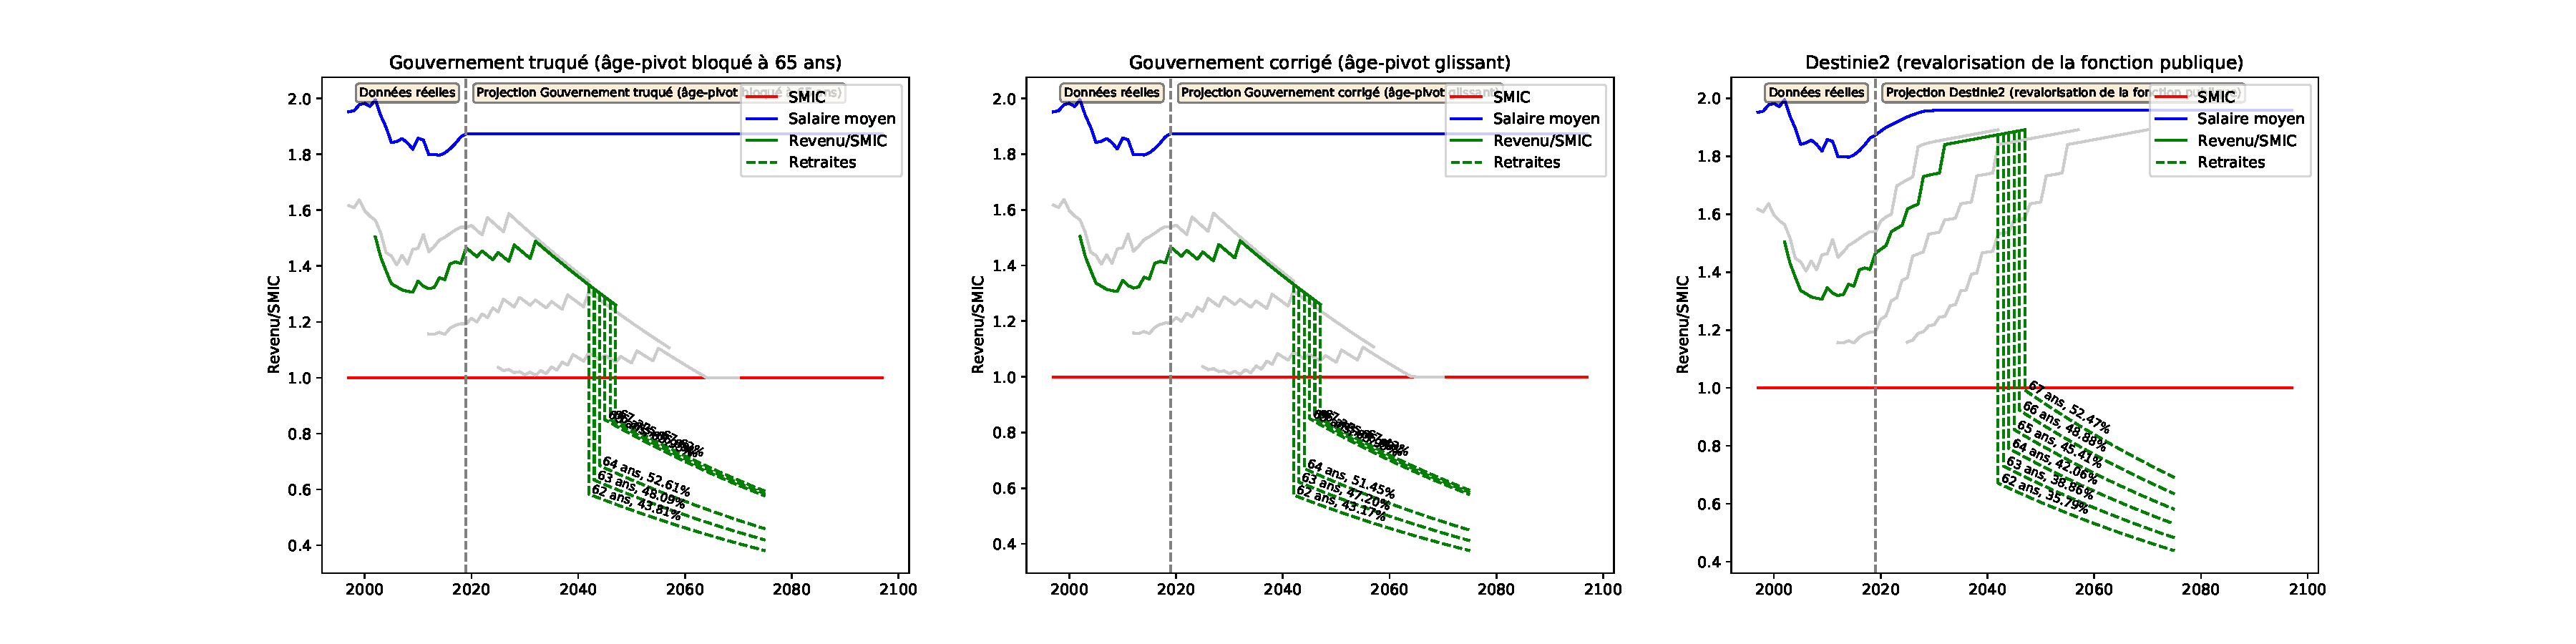
\includegraphics[width=0.9\textwidth]{fig/TechHosp_1980_22_dest_retraite.pdf}\end{center} \label{fig/TechHosp_1980_22_dest_retraite.pdf} 

\newpage 
 
\subsection{Génération 1990 (début en 2012)} 

\paragraph{Retraites possibles et ratios Revenu/SMIC à 70, 75, 80, 85, 90 ans avec le modèle \emph{Gouvernement truqué (âge-pivot bloqué à 65 ans)}}  
 
{ \scriptsize \begin{center} 
\begin{tabular}[htb]{|c|c||c|c||c|c||c||c|c|c|c|c|c|} 
\hline 
 Retraite en &  Âge &  Âge pivot &  Décote/Surcote &  Retraite (\euro{} 2019) &  Tx Rempl(\%) &  SMIC (\euro{} 2019) &  Retraite/SMIC &  Rev70/SMIC &  Rev75/SMIC &  Rev80/SMIC &  Rev85/SMIC &  Rev90/SMIC \\ 
\hline \hline 
 2052 &  62 &  65 ans 0 mois &  -15.00\% &  1431.21 &  {\bf 46.99} &  2601.14 &  {\bf {\color{red} 0.55}} &  {\bf {\color{red} 0.50}} &  {\bf {\color{red} 0.47}} &  {\bf {\color{red} 0.44}} &  {\bf {\color{red} 0.41}} &  {\bf {\color{red} 0.38}} \\ 
\hline 
 2053 &  63 &  65 ans 0 mois &  -10.00\% &  1573.33 &  {\bf 51.56} &  2634.96 &  {\bf {\color{red} 0.60}} &  {\bf {\color{red} 0.55}} &  {\bf {\color{red} 0.51}} &  {\bf {\color{red} 0.48}} &  {\bf {\color{red} 0.45}} &  {\bf {\color{red} 0.42}} \\ 
\hline 
 2054 &  64 &  65 ans 0 mois &  -5.00\% &  1722.75 &  {\bf 56.35} &  2669.21 &  {\bf {\color{red} 0.65}} &  {\bf {\color{red} 0.60}} &  {\bf {\color{red} 0.56}} &  {\bf {\color{red} 0.52}} &  {\bf {\color{red} 0.49}} &  {\bf {\color{red} 0.46}} \\ 
\hline 
 2055 &  65 &  65 ans 0 mois &  0.00\% &  2298.33 &  {\bf 75.04} &  2703.91 &  {\bf {\color{red} 0.85}} &  {\bf {\color{red} 0.80}} &  {\bf {\color{red} 0.75}} &  {\bf {\color{red} 0.70}} &  {\bf {\color{red} 0.66}} &  {\bf {\color{red} 0.62}} \\ 
\hline 
 2056 &  66 &  65 ans 0 mois &  5.00\% &  2328.20 &  {\bf 75.88} &  2739.06 &  {\bf {\color{red} 0.85}} &  {\bf {\color{red} 0.81}} &  {\bf {\color{red} 0.76}} &  {\bf {\color{red} 0.71}} &  {\bf {\color{red} 0.67}} &  {\bf {\color{red} 0.62}} \\ 
\hline 
 2057 &  67 &  65 ans 0 mois &  10.00\% &  2358.47 &  {\bf 76.73} &  2774.67 &  {\bf {\color{red} 0.85}} &  {\bf {\color{red} 0.82}} &  {\bf {\color{red} 0.77}} &  {\bf {\color{red} 0.72}} &  {\bf {\color{red} 0.67}} &  {\bf {\color{red} 0.63}} \\ 
\hline 
\hline 
\end{tabular} 
\end{center} } 
\paragraph{Retraites possibles et ratios Revenu/SMIC à 70, 75, 80, 85, 90 ans avec le modèle \emph{Gouvernement corrigé (âge-pivot glissant)}}  
 
{ \scriptsize \begin{center} 
\begin{tabular}[htb]{|c|c||c|c||c|c||c||c|c|c|c|c|c|} 
\hline 
 Retraite en &  Âge &  Âge pivot &  Décote/Surcote &  Retraite (\euro{} 2019) &  Tx Rempl(\%) &  SMIC (\euro{} 2019) &  Retraite/SMIC &  Rev70/SMIC &  Rev75/SMIC &  Rev80/SMIC &  Rev85/SMIC &  Rev90/SMIC \\ 
\hline \hline 
 2052 &  62 &  66 ans 1 mois &  -20.42\% &  1340.01 &  {\bf 43.99} &  2601.14 &  {\bf {\color{red} 0.52}} &  {\bf {\color{red} 0.46}} &  {\bf {\color{red} 0.44}} &  {\bf {\color{red} 0.41}} &  {\bf {\color{red} 0.38}} &  {\bf {\color{red} 0.36}} \\ 
\hline 
 2053 &  63 &  66 ans 2 mois &  -15.83\% &  1471.36 &  {\bf 48.22} &  2634.96 &  {\bf {\color{red} 0.56}} &  {\bf {\color{red} 0.51}} &  {\bf {\color{red} 0.48}} &  {\bf {\color{red} 0.45}} &  {\bf {\color{red} 0.42}} &  {\bf {\color{red} 0.39}} \\ 
\hline 
 2054 &  64 &  66 ans 3 mois &  -11.25\% &  1609.41 &  {\bf 52.64} &  2669.21 &  {\bf {\color{red} 0.60}} &  {\bf {\color{red} 0.56}} &  {\bf {\color{red} 0.52}} &  {\bf {\color{red} 0.49}} &  {\bf {\color{red} 0.46}} &  {\bf {\color{red} 0.43}} \\ 
\hline 
 2055 &  65 &  66 ans 4 mois &  -6.67\% &  2298.33 &  {\bf 75.04} &  2703.91 &  {\bf {\color{red} 0.85}} &  {\bf {\color{red} 0.80}} &  {\bf {\color{red} 0.75}} &  {\bf {\color{red} 0.70}} &  {\bf {\color{red} 0.66}} &  {\bf {\color{red} 0.62}} \\ 
\hline 
 2056 &  66 &  66 ans 5 mois &  -2.08\% &  2328.20 &  {\bf 75.88} &  2739.06 &  {\bf {\color{red} 0.85}} &  {\bf {\color{red} 0.81}} &  {\bf {\color{red} 0.76}} &  {\bf {\color{red} 0.71}} &  {\bf {\color{red} 0.67}} &  {\bf {\color{red} 0.62}} \\ 
\hline 
 2057 &  67 &  66 ans 6 mois &  2.50\% &  2358.47 &  {\bf 76.73} &  2774.67 &  {\bf {\color{red} 0.85}} &  {\bf {\color{red} 0.82}} &  {\bf {\color{red} 0.77}} &  {\bf {\color{red} 0.72}} &  {\bf {\color{red} 0.67}} &  {\bf {\color{red} 0.63}} \\ 
\hline 
\hline 
\end{tabular} 
\end{center} } 
\paragraph{Retraites possibles et ratios Revenu/SMIC à 70, 75, 80, 85, 90 ans avec le modèle \emph{Destinie2 (revalorisation de la fonction publique)}}  
 
{ \scriptsize \begin{center} 
\begin{tabular}[htb]{|c|c||c|c||c|c||c||c|c|c|c|c|c|} 
\hline 
 Retraite en &  Âge &  Âge pivot &  Décote/Surcote &  Retraite (\euro{} 2019) &  Tx Rempl(\%) &  SMIC (\euro{} 2019) &  Retraite/SMIC &  Rev70/SMIC &  Rev75/SMIC &  Rev80/SMIC &  Rev85/SMIC &  Rev90/SMIC \\ 
\hline \hline 
 2052 &  62 &  66 ans 1 mois &  -20.42\% &  1675.64 &  {\bf 36.35} &  2445.56 &  {\bf {\color{red} 0.69}} &  {\bf {\color{red} 0.62}} &  {\bf {\color{red} 0.58}} &  {\bf {\color{red} 0.54}} &  {\bf {\color{red} 0.51}} &  {\bf {\color{red} 0.48}} \\ 
\hline 
 2053 &  63 &  66 ans 2 mois &  -15.83\% &  1849.89 &  {\bf 39.62} &  2477.35 &  {\bf {\color{red} 0.75}} &  {\bf {\color{red} 0.68}} &  {\bf {\color{red} 0.64}} &  {\bf {\color{red} 0.60}} &  {\bf {\color{red} 0.56}} &  {\bf {\color{red} 0.53}} \\ 
\hline 
 2054 &  64 &  66 ans 3 mois &  -11.25\% &  2034.42 &  {\bf 43.01} &  2509.56 &  {\bf {\color{red} 0.81}} &  {\bf {\color{red} 0.75}} &  {\bf {\color{red} 0.70}} &  {\bf {\color{red} 0.66}} &  {\bf {\color{red} 0.62}} &  {\bf {\color{red} 0.58}} \\ 
\hline 
 2055 &  65 &  66 ans 4 mois &  -6.67\% &  2229.55 &  {\bf 46.53} &  2542.18 &  {\bf {\color{red} 0.88}} &  {\bf {\color{red} 0.82}} &  {\bf {\color{red} 0.77}} &  {\bf {\color{red} 0.72}} &  {\bf {\color{red} 0.68}} &  {\bf {\color{red} 0.64}} \\ 
\hline 
 2056 &  66 &  66 ans 5 mois &  -2.08\% &  2435.60 &  {\bf 50.18} &  2575.23 &  {\bf {\color{red} 0.95}} &  {\bf {\color{red} 0.90}} &  {\bf {\color{red} 0.84}} &  {\bf {\color{red} 0.79}} &  {\bf {\color{red} 0.74}} &  {\bf {\color{red} 0.69}} \\ 
\hline 
 2057 &  67 &  66 ans 6 mois &  2.50\% &  2652.91 &  {\bf 53.95} &  2608.71 &  {\bf 1.02} &  {\bf {\color{red} 0.98}} &  {\bf {\color{red} 0.92}} &  {\bf {\color{red} 0.86}} &  {\bf {\color{red} 0.81}} &  {\bf {\color{red} 0.76}} \\ 
\hline 
\hline 
\end{tabular} 
\end{center} } 

 \begin{center}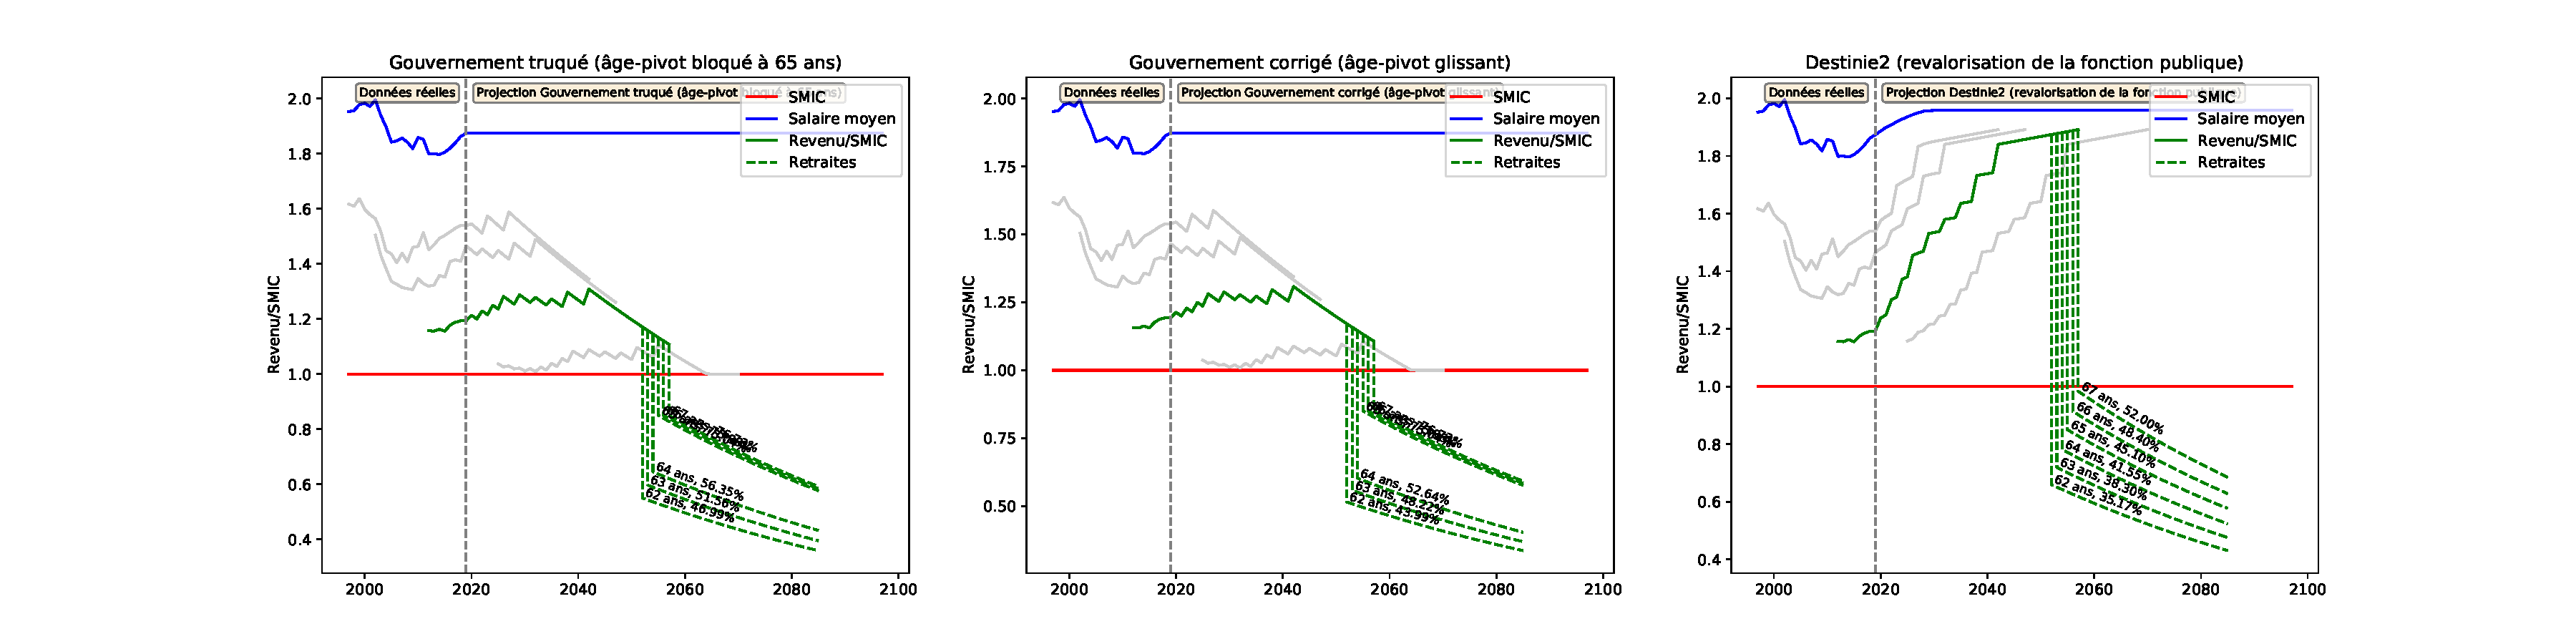
\includegraphics[width=0.9\textwidth]{fig/TechHosp_1990_22_dest_retraite.pdf}\end{center} \label{fig/TechHosp_1990_22_dest_retraite.pdf} 

\newpage 
 
\subsection{Génération 2003 (début en 2025)} 

\paragraph{Retraites possibles et ratios Revenu/SMIC à 70, 75, 80, 85, 90 ans avec le modèle \emph{Gouvernement truqué (âge-pivot bloqué à 65 ans)}}  
 
{ \scriptsize \begin{center} 
\begin{tabular}[htb]{|c|c||c|c||c|c||c||c|c|c|c|c|c|} 
\hline 
 Retraite en &  Âge &  Âge pivot &  Décote/Surcote &  Retraite (\euro{} 2019) &  Tx Rempl(\%) &  SMIC (\euro{} 2019) &  Retraite/SMIC &  Rev70/SMIC &  Rev75/SMIC &  Rev80/SMIC &  Rev85/SMIC &  Rev90/SMIC \\ 
\hline \hline 
 2065 &  62 &  65 ans 0 mois &  -15.00\% &  1531.73 &  {\bf 49.78} &  3076.71 &  {\bf {\color{red} 0.50}} &  {\bf {\color{red} 0.45}} &  {\bf {\color{red} 0.42}} &  {\bf {\color{red} 0.39}} &  {\bf {\color{red} 0.37}} &  {\bf {\color{red} 0.35}} \\ 
\hline 
 2066 &  63 &  65 ans 0 mois &  -10.00\% &  1681.96 &  {\bf 53.97} &  3116.71 &  {\bf {\color{red} 0.54}} &  {\bf {\color{red} 0.49}} &  {\bf {\color{red} 0.46}} &  {\bf {\color{red} 0.43}} &  {\bf {\color{red} 0.41}} &  {\bf {\color{red} 0.38}} \\ 
\hline 
 2067 &  64 &  65 ans 0 mois &  -5.00\% &  1840.23 &  {\bf 58.29} &  3157.23 &  {\bf {\color{red} 0.58}} &  {\bf {\color{red} 0.54}} &  {\bf {\color{red} 0.51}} &  {\bf {\color{red} 0.47}} &  {\bf {\color{red} 0.44}} &  {\bf {\color{red} 0.42}} \\ 
\hline 
 2068 &  65 &  65 ans 0 mois &  0.00\% &  2718.53 &  {\bf 85.00} &  3198.27 &  {\bf {\color{red} 0.85}} &  {\bf {\color{red} 0.80}} &  {\bf {\color{red} 0.75}} &  {\bf {\color{red} 0.70}} &  {\bf {\color{red} 0.66}} &  {\bf {\color{red} 0.62}} \\ 
\hline 
 2069 &  66 &  65 ans 0 mois &  5.00\% &  2753.87 &  {\bf 85.00} &  3239.85 &  {\bf {\color{red} 0.85}} &  {\bf {\color{red} 0.81}} &  {\bf {\color{red} 0.76}} &  {\bf {\color{red} 0.71}} &  {\bf {\color{red} 0.67}} &  {\bf {\color{red} 0.62}} \\ 
\hline 
 2070 &  67 &  65 ans 0 mois &  10.00\% &  2789.67 &  {\bf 85.00} &  3281.97 &  {\bf {\color{red} 0.85}} &  {\bf {\color{red} 0.82}} &  {\bf {\color{red} 0.77}} &  {\bf {\color{red} 0.72}} &  {\bf {\color{red} 0.67}} &  {\bf {\color{red} 0.63}} \\ 
\hline 
\hline 
\end{tabular} 
\end{center} } 
\paragraph{Retraites possibles et ratios Revenu/SMIC à 70, 75, 80, 85, 90 ans avec le modèle \emph{Gouvernement corrigé (âge-pivot glissant)}}  
 
{ \scriptsize \begin{center} 
\begin{tabular}[htb]{|c|c||c|c||c|c||c||c|c|c|c|c|c|} 
\hline 
 Retraite en &  Âge &  Âge pivot &  Décote/Surcote &  Retraite (\euro{} 2019) &  Tx Rempl(\%) &  SMIC (\euro{} 2019) &  Retraite/SMIC &  Rev70/SMIC &  Rev75/SMIC &  Rev80/SMIC &  Rev85/SMIC &  Rev90/SMIC \\ 
\hline \hline 
 2065 &  62 &  67 ans 2 mois &  -25.83\% &  1336.51 &  {\bf 43.44} &  3076.71 &  {\bf {\color{red} 0.43}} &  {\bf {\color{red} 0.39}} &  {\bf {\color{red} 0.37}} &  {\bf {\color{red} 0.34}} &  {\bf {\color{red} 0.32}} &  {\bf {\color{red} 0.30}} \\ 
\hline 
 2066 &  63 &  67 ans 3 mois &  -21.25\% &  1471.71 &  {\bf 47.22} &  3116.71 &  {\bf {\color{red} 0.47}} &  {\bf {\color{red} 0.43}} &  {\bf {\color{red} 0.40}} &  {\bf {\color{red} 0.38}} &  {\bf {\color{red} 0.36}} &  {\bf {\color{red} 0.33}} \\ 
\hline 
 2067 &  64 &  67 ans 4 mois &  -16.67\% &  1614.24 &  {\bf 51.13} &  3157.23 &  {\bf {\color{red} 0.51}} &  {\bf {\color{red} 0.47}} &  {\bf {\color{red} 0.44}} &  {\bf {\color{red} 0.42}} &  {\bf {\color{red} 0.39}} &  {\bf {\color{red} 0.37}} \\ 
\hline 
 2068 &  65 &  67 ans 5 mois &  -12.08\% &  2718.53 &  {\bf 85.00} &  3198.27 &  {\bf {\color{red} 0.85}} &  {\bf {\color{red} 0.80}} &  {\bf {\color{red} 0.75}} &  {\bf {\color{red} 0.70}} &  {\bf {\color{red} 0.66}} &  {\bf {\color{red} 0.62}} \\ 
\hline 
 2069 &  66 &  67 ans 6 mois &  -7.50\% &  2753.87 &  {\bf 85.00} &  3239.85 &  {\bf {\color{red} 0.85}} &  {\bf {\color{red} 0.81}} &  {\bf {\color{red} 0.76}} &  {\bf {\color{red} 0.71}} &  {\bf {\color{red} 0.67}} &  {\bf {\color{red} 0.62}} \\ 
\hline 
 2070 &  67 &  67 ans 7 mois &  -2.92\% &  2789.67 &  {\bf 85.00} &  3281.97 &  {\bf {\color{red} 0.85}} &  {\bf {\color{red} 0.82}} &  {\bf {\color{red} 0.77}} &  {\bf {\color{red} 0.72}} &  {\bf {\color{red} 0.67}} &  {\bf {\color{red} 0.63}} \\ 
\hline 
\hline 
\end{tabular} 
\end{center} } 
\paragraph{Retraites possibles et ratios Revenu/SMIC à 70, 75, 80, 85, 90 ans avec le modèle \emph{Destinie2 (revalorisation de la fonction publique)}}  
 
{ \scriptsize \begin{center} 
\begin{tabular}[htb]{|c|c||c|c||c|c||c||c|c|c|c|c|c|} 
\hline 
 Retraite en &  Âge &  Âge pivot &  Décote/Surcote &  Retraite (\euro{} 2019) &  Tx Rempl(\%) &  SMIC (\euro{} 2019) &  Retraite/SMIC &  Rev70/SMIC &  Rev75/SMIC &  Rev80/SMIC &  Rev85/SMIC &  Rev90/SMIC \\ 
\hline \hline 
 2065 &  62 &  67 ans 2 mois &  -25.83\% &  1942.90 &  {\bf 35.63} &  2892.68 &  {\bf {\color{red} 0.67}} &  {\bf {\color{red} 0.61}} &  {\bf {\color{red} 0.57}} &  {\bf {\color{red} 0.53}} &  {\bf {\color{red} 0.50}} &  {\bf {\color{red} 0.47}} \\ 
\hline 
 2066 &  63 &  67 ans 3 mois &  -21.25\% &  2150.33 &  {\bf 38.93} &  2930.29 &  {\bf {\color{red} 0.73}} &  {\bf {\color{red} 0.67}} &  {\bf {\color{red} 0.63}} &  {\bf {\color{red} 0.59}} &  {\bf {\color{red} 0.55}} &  {\bf {\color{red} 0.52}} \\ 
\hline 
 2067 &  64 &  67 ans 4 mois &  -16.67\% &  2369.96 &  {\bf 42.36} &  2968.38 &  {\bf {\color{red} 0.80}} &  {\bf {\color{red} 0.74}} &  {\bf {\color{red} 0.69}} &  {\bf {\color{red} 0.65}} &  {\bf {\color{red} 0.61}} &  {\bf {\color{red} 0.57}} \\ 
\hline 
 2068 &  65 &  67 ans 5 mois &  -12.08\% &  2602.17 &  {\bf 45.91} &  3006.97 &  {\bf {\color{red} 0.87}} &  {\bf {\color{red} 0.81}} &  {\bf {\color{red} 0.76}} &  {\bf {\color{red} 0.71}} &  {\bf {\color{red} 0.67}} &  {\bf {\color{red} 0.63}} \\ 
\hline 
 2069 &  66 &  67 ans 6 mois &  -7.50\% &  2847.34 &  {\bf 49.59} &  3046.06 &  {\bf {\color{red} 0.93}} &  {\bf {\color{red} 0.89}} &  {\bf {\color{red} 0.83}} &  {\bf {\color{red} 0.78}} &  {\bf {\color{red} 0.73}} &  {\bf {\color{red} 0.69}} \\ 
\hline 
 2070 &  67 &  67 ans 7 mois &  -2.92\% &  3105.87 &  {\bf 53.40} &  3085.66 &  {\bf 1.01} &  {\bf {\color{red} 0.97}} &  {\bf {\color{red} 0.91}} &  {\bf {\color{red} 0.85}} &  {\bf {\color{red} 0.80}} &  {\bf {\color{red} 0.75}} \\ 
\hline 
\hline 
\end{tabular} 
\end{center} } 

 \begin{center}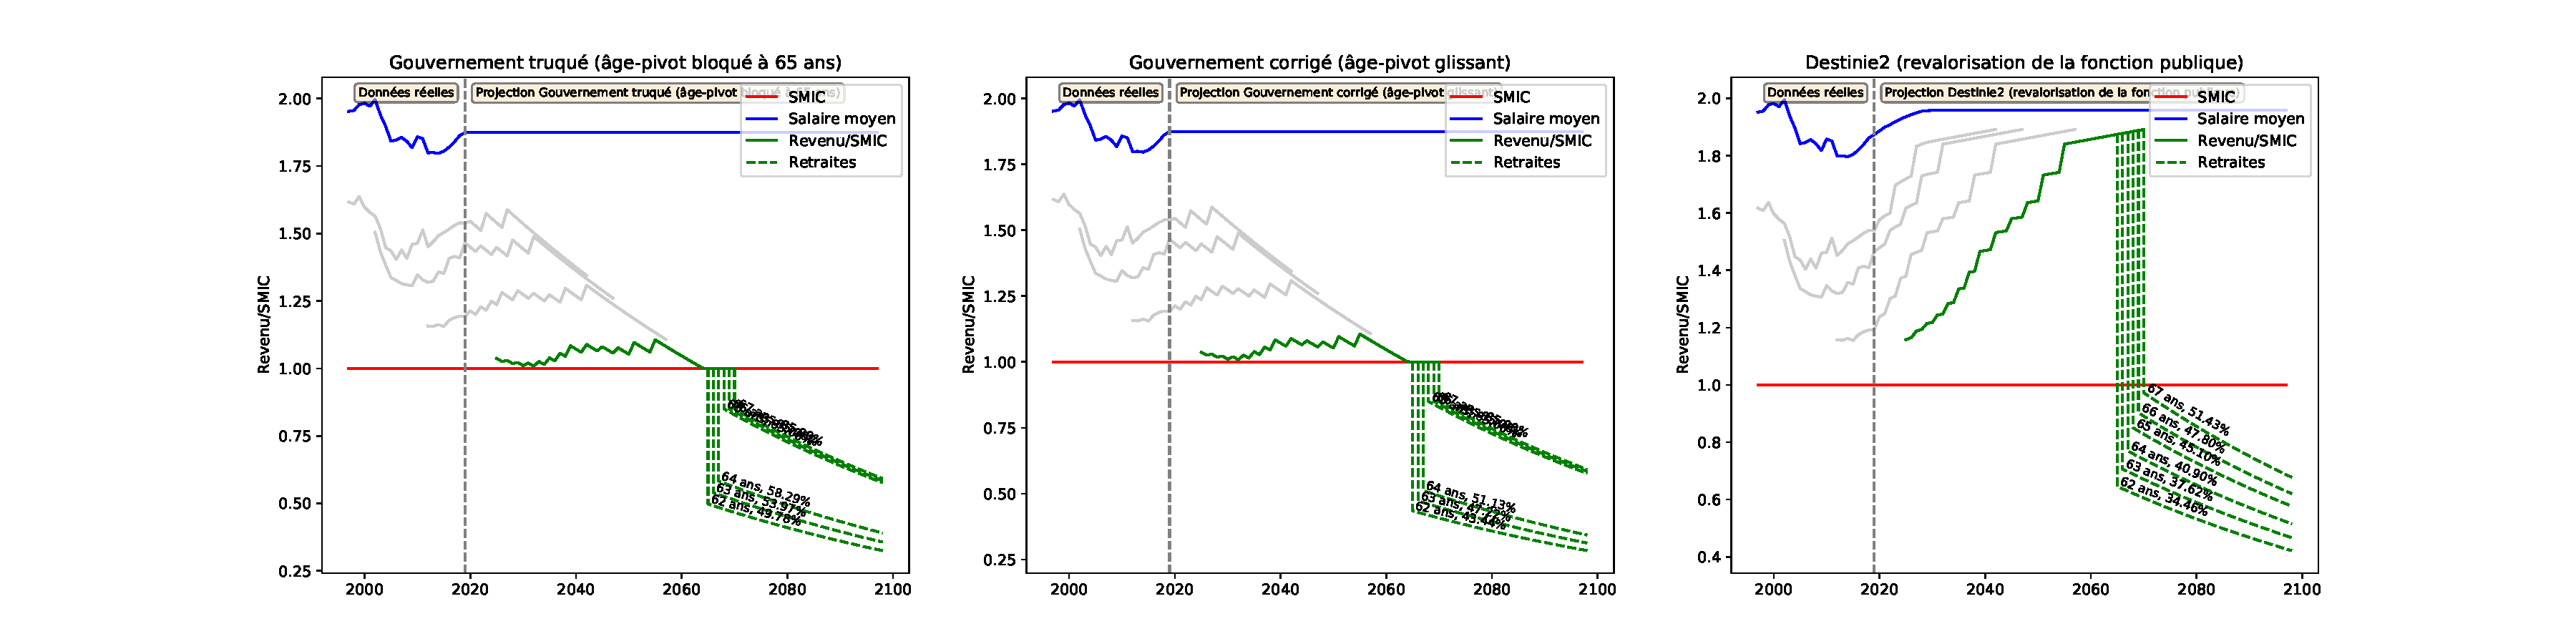
\includegraphics[width=0.9\textwidth]{fig/TechHosp_2003_22_dest_retraite.pdf}\end{center} \label{fig/TechHosp_2003_22_dest_retraite.pdf} 

\newpage 
 
\chapter{Adjoint Technique (devenant principal C2 puis C1)} 

\begin{minipage}{0.55\linewidth}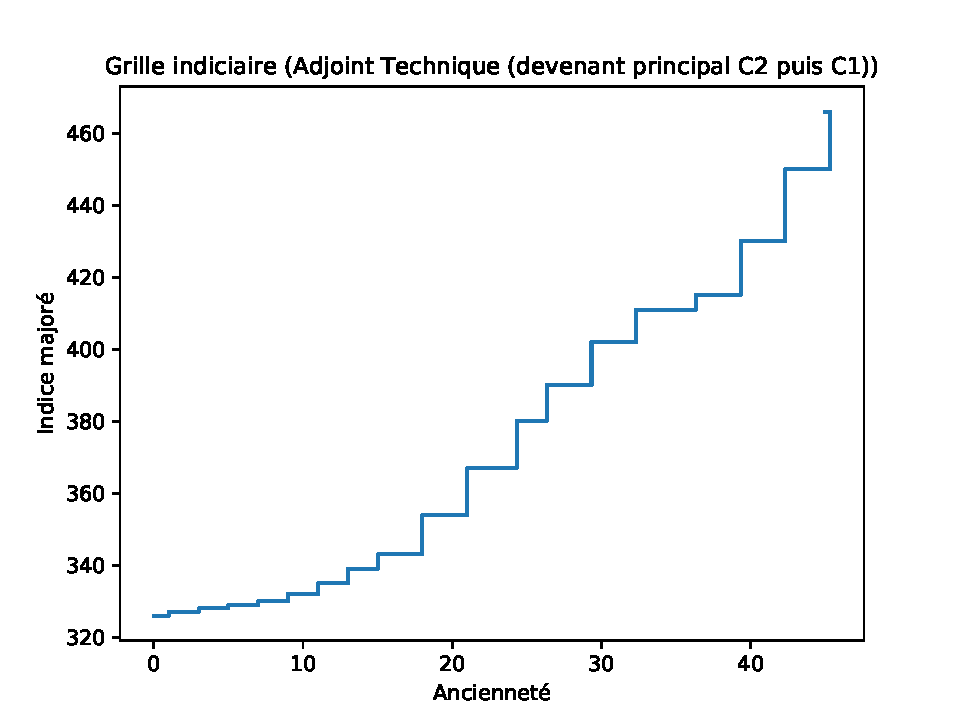
\includegraphics[width=0.7\textwidth]{fig/grille_AdjTech.pdf}\end{minipage} 
\begin{minipage}{0.3\linewidth} 
 \begin{center} 

\begin{tabular}[htb]{|c|c|} 
\hline 
 Indice majoré &  Durée (années) \\ 
\hline \hline 
 326 &  1.00 \\ 
\hline 
 327 &  2.00 \\ 
\hline 
 328 &  2.00 \\ 
\hline 
 329 &  2.00 \\ 
\hline 
 330 &  2.00 \\ 
\hline 
 332 &  2.00 \\ 
\hline 
 335 &  2.00 \\ 
\hline 
 339 &  2.00 \\ 
\hline 
 343 &  3.00 \\ 
\hline 
 354 &  3.00 \\ 
\hline 
 367 &  3.33 \\ 
\hline 
 380 &  2.00 \\ 
\hline 
 390 &  3.00 \\ 
\hline 
 402 &  3.00 \\ 
\hline 
 411 &  4.00 \\ 
\hline 
 415 &  3.00 \\ 
\hline 
 430 &  3.00 \\ 
\hline 
 450 &  3.00 \\ 
\hline 
 466 &   \\ 
\hline 
\hline 
\end{tabular} 
\end{center} 
 \end{minipage} 


 \addto{\captionsenglish}{ \renewcommand{\mtctitle}{}} \setcounter{minitocdepth}{2} 
 \minitoc \newpage 

\section{Début de carrière à 22 ans} 

\subsection{Génération 1975 (début en 1997)} 

\paragraph{Retraites possibles et ratios Revenu/SMIC à 70, 75, 80, 85, 90 ans avec le modèle \emph{Gouvernement truqué (âge-pivot bloqué à 65 ans)}}  
 
{ \scriptsize \begin{center} 
\begin{tabular}[htb]{|c|c||c|c||c|c||c||c|c|c|c|c|c|} 
\hline 
 Retraite en &  Âge &  Âge pivot &  Décote/Surcote &  Retraite (\euro{} 2019) &  Tx Rempl(\%) &  SMIC (\euro{} 2019) &  Retraite/SMIC &  Rev70/SMIC &  Rev75/SMIC &  Rev80/SMIC &  Rev85/SMIC &  Rev90/SMIC \\ 
\hline \hline 
 2037 &  62 &  64 ans 10 mois &  -14.17\% &  1091.14 &  {\bf 43.52} &  2143.00 &  {\bf {\color{red} 0.51}} &  {\bf {\color{red} 0.46}} &  {\bf {\color{red} 0.43}} &  {\bf {\color{red} 0.40}} &  {\bf {\color{red} 0.38}} &  {\bf {\color{red} 0.35}} \\ 
\hline 
 2038 &  63 &  64 ans 11 mois &  -9.58\% &  1189.79 &  {\bf 47.37} &  2170.86 &  {\bf {\color{red} 0.55}} &  {\bf {\color{red} 0.50}} &  {\bf {\color{red} 0.47}} &  {\bf {\color{red} 0.44}} &  {\bf {\color{red} 0.41}} &  {\bf {\color{red} 0.39}} \\ 
\hline 
 2039 &  64 &  65 ans 0 mois &  -5.00\% &  1294.91 &  {\bf 49.90} &  2199.08 &  {\bf {\color{red} 0.59}} &  {\bf {\color{red} 0.54}} &  {\bf {\color{red} 0.51}} &  {\bf {\color{red} 0.48}} &  {\bf {\color{red} 0.45}} &  {\bf {\color{red} 0.42}} \\ 
\hline 
 2040 &  65 &  65 ans 0 mois &  0.00\% &  1893.52 &  {\bf 71.76} &  2227.67 &  {\bf {\color{red} 0.85}} &  {\bf {\color{red} 0.80}} &  {\bf {\color{red} 0.75}} &  {\bf {\color{red} 0.70}} &  {\bf {\color{red} 0.66}} &  {\bf {\color{red} 0.62}} \\ 
\hline 
 2041 &  66 &  65 ans 0 mois &  5.00\% &  1918.14 &  {\bf 72.56} &  2256.63 &  {\bf {\color{red} 0.85}} &  {\bf {\color{red} 0.81}} &  {\bf {\color{red} 0.76}} &  {\bf {\color{red} 0.71}} &  {\bf {\color{red} 0.67}} &  {\bf {\color{red} 0.62}} \\ 
\hline 
 2042 &  67 &  65 ans 0 mois &  10.00\% &  1943.07 &  {\bf 71.66} &  2285.97 &  {\bf {\color{red} 0.85}} &  {\bf {\color{red} 0.82}} &  {\bf {\color{red} 0.77}} &  {\bf {\color{red} 0.72}} &  {\bf {\color{red} 0.67}} &  {\bf {\color{red} 0.63}} \\ 
\hline 
\hline 
\end{tabular} 
\end{center} } 
\paragraph{Retraites possibles et ratios Revenu/SMIC à 70, 75, 80, 85, 90 ans avec le modèle \emph{Gouvernement corrigé (âge-pivot glissant)}}  
 
{ \scriptsize \begin{center} 
\begin{tabular}[htb]{|c|c||c|c||c|c||c||c|c|c|c|c|c|} 
\hline 
 Retraite en &  Âge &  Âge pivot &  Décote/Surcote &  Retraite (\euro{} 2019) &  Tx Rempl(\%) &  SMIC (\euro{} 2019) &  Retraite/SMIC &  Rev70/SMIC &  Rev75/SMIC &  Rev80/SMIC &  Rev85/SMIC &  Rev90/SMIC \\ 
\hline \hline 
 2037 &  62 &  64 ans 10 mois &  -14.17\% &  1091.14 &  {\bf 43.52} &  2143.00 &  {\bf {\color{red} 0.51}} &  {\bf {\color{red} 0.46}} &  {\bf {\color{red} 0.43}} &  {\bf {\color{red} 0.40}} &  {\bf {\color{red} 0.38}} &  {\bf {\color{red} 0.35}} \\ 
\hline 
 2038 &  63 &  64 ans 11 mois &  -9.58\% &  1189.79 &  {\bf 47.37} &  2170.86 &  {\bf {\color{red} 0.55}} &  {\bf {\color{red} 0.50}} &  {\bf {\color{red} 0.47}} &  {\bf {\color{red} 0.44}} &  {\bf {\color{red} 0.41}} &  {\bf {\color{red} 0.39}} \\ 
\hline 
 2039 &  64 &  65 ans 0 mois &  -5.00\% &  1294.91 &  {\bf 49.90} &  2199.08 &  {\bf {\color{red} 0.59}} &  {\bf {\color{red} 0.54}} &  {\bf {\color{red} 0.51}} &  {\bf {\color{red} 0.48}} &  {\bf {\color{red} 0.45}} &  {\bf {\color{red} 0.42}} \\ 
\hline 
 2040 &  65 &  65 ans 1 mois &  -0.42\% &  1893.52 &  {\bf 71.76} &  2227.67 &  {\bf {\color{red} 0.85}} &  {\bf {\color{red} 0.80}} &  {\bf {\color{red} 0.75}} &  {\bf {\color{red} 0.70}} &  {\bf {\color{red} 0.66}} &  {\bf {\color{red} 0.62}} \\ 
\hline 
 2041 &  66 &  65 ans 2 mois &  4.17\% &  1918.14 &  {\bf 72.56} &  2256.63 &  {\bf {\color{red} 0.85}} &  {\bf {\color{red} 0.81}} &  {\bf {\color{red} 0.76}} &  {\bf {\color{red} 0.71}} &  {\bf {\color{red} 0.67}} &  {\bf {\color{red} 0.62}} \\ 
\hline 
 2042 &  67 &  65 ans 3 mois &  8.75\% &  1943.07 &  {\bf 71.66} &  2285.97 &  {\bf {\color{red} 0.85}} &  {\bf {\color{red} 0.82}} &  {\bf {\color{red} 0.77}} &  {\bf {\color{red} 0.72}} &  {\bf {\color{red} 0.67}} &  {\bf {\color{red} 0.63}} \\ 
\hline 
\hline 
\end{tabular} 
\end{center} } 
\paragraph{Retraites possibles et ratios Revenu/SMIC à 70, 75, 80, 85, 90 ans avec le modèle \emph{Destinie2 (revalorisation de la fonction publique)}}  
 
{ \scriptsize \begin{center} 
\begin{tabular}[htb]{|c|c||c|c||c|c||c||c|c|c|c|c|c|} 
\hline 
 Retraite en &  Âge &  Âge pivot &  Décote/Surcote &  Retraite (\euro{} 2019) &  Tx Rempl(\%) &  SMIC (\euro{} 2019) &  Retraite/SMIC &  Rev70/SMIC &  Rev75/SMIC &  Rev80/SMIC &  Rev85/SMIC &  Rev90/SMIC \\ 
\hline \hline 
 2037 &  62 &  64 ans 10 mois &  -14.17\% &  1212.60 &  {\bf 38.79} &  2014.82 &  {\bf {\color{red} 0.60}} &  {\bf {\color{red} 0.54}} &  {\bf {\color{red} 0.51}} &  {\bf {\color{red} 0.48}} &  {\bf {\color{red} 0.45}} &  {\bf {\color{red} 0.42}} \\ 
\hline 
 2038 &  63 &  64 ans 11 mois &  -9.58\% &  1326.95 &  {\bf 41.90} &  2041.01 &  {\bf {\color{red} 0.65}} &  {\bf {\color{red} 0.59}} &  {\bf {\color{red} 0.56}} &  {\bf {\color{red} 0.52}} &  {\bf {\color{red} 0.49}} &  {\bf {\color{red} 0.46}} \\ 
\hline 
 2039 &  64 &  65 ans 0 mois &  -5.00\% &  1449.66 &  {\bf 43.82} &  2067.55 &  {\bf {\color{red} 0.70}} &  {\bf {\color{red} 0.65}} &  {\bf {\color{red} 0.61}} &  {\bf {\color{red} 0.57}} &  {\bf {\color{red} 0.53}} &  {\bf {\color{red} 0.50}} \\ 
\hline 
 2040 &  65 &  65 ans 1 mois &  -0.42\% &  1780.26 &  {\bf 52.34} &  2094.43 &  {\bf {\color{red} 0.85}} &  {\bf {\color{red} 0.80}} &  {\bf {\color{red} 0.75}} &  {\bf {\color{red} 0.70}} &  {\bf {\color{red} 0.66}} &  {\bf {\color{red} 0.62}} \\ 
\hline 
 2041 &  66 &  65 ans 2 mois &  4.17\% &  1803.40 &  {\bf 52.34} &  2121.65 &  {\bf {\color{red} 0.85}} &  {\bf {\color{red} 0.81}} &  {\bf {\color{red} 0.76}} &  {\bf {\color{red} 0.71}} &  {\bf {\color{red} 0.67}} &  {\bf {\color{red} 0.62}} \\ 
\hline 
 2042 &  67 &  65 ans 3 mois &  8.75\% &  1868.74 &  {\bf 52.30} &  2149.23 &  {\bf {\color{red} 0.87}} &  {\bf {\color{red} 0.84}} &  {\bf {\color{red} 0.78}} &  {\bf {\color{red} 0.74}} &  {\bf {\color{red} 0.69}} &  {\bf {\color{red} 0.65}} \\ 
\hline 
\hline 
\end{tabular} 
\end{center} } 

 \begin{center}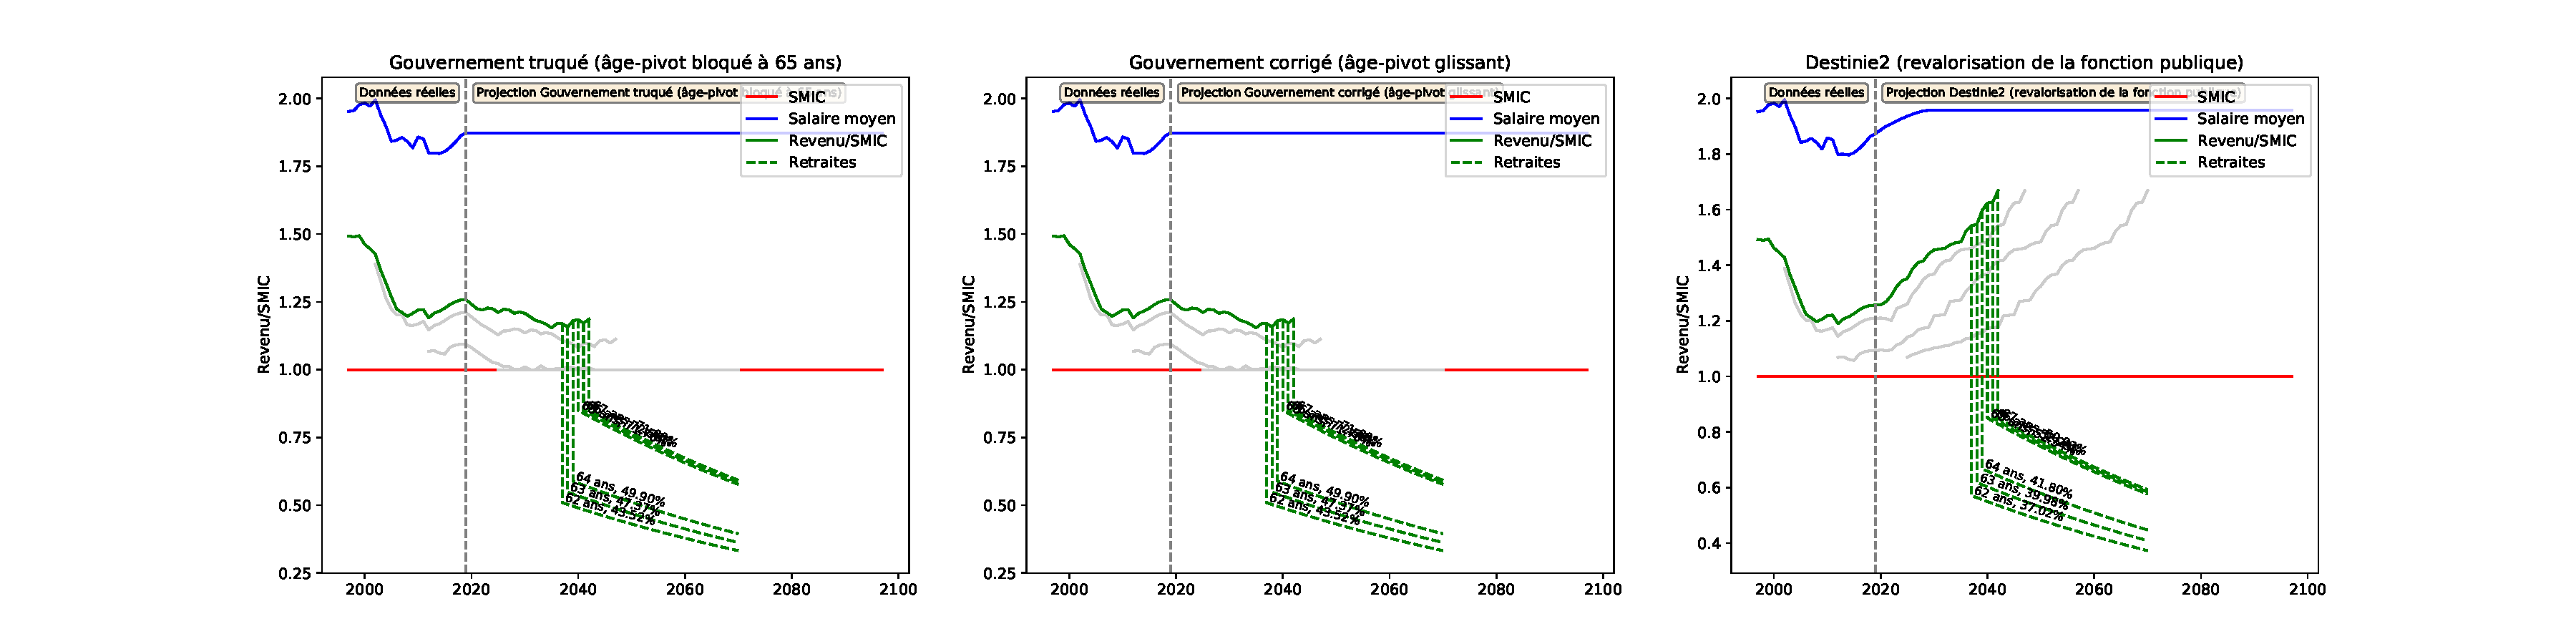
\includegraphics[width=0.9\textwidth]{fig/AdjTech_1975_22_dest_retraite.pdf}\end{center} \label{fig/AdjTech_1975_22_dest_retraite.pdf} 

\newpage 
 
\subsection{Génération 1980 (début en 2002)} 

\paragraph{Retraites possibles et ratios Revenu/SMIC à 70, 75, 80, 85, 90 ans avec le modèle \emph{Gouvernement truqué (âge-pivot bloqué à 65 ans)}}  
 
{ \scriptsize \begin{center} 
\begin{tabular}[htb]{|c|c||c|c||c|c||c||c|c|c|c|c|c|} 
\hline 
 Retraite en &  Âge &  Âge pivot &  Décote/Surcote &  Retraite (\euro{} 2019) &  Tx Rempl(\%) &  SMIC (\euro{} 2019) &  Retraite/SMIC &  Rev70/SMIC &  Rev75/SMIC &  Rev80/SMIC &  Rev85/SMIC &  Rev90/SMIC \\ 
\hline \hline 
 2042 &  62 &  65 ans 0 mois &  -15.00\% &  1105.27 &  {\bf 44.09} &  2285.97 &  {\bf {\color{red} 0.48}} &  {\bf {\color{red} 0.44}} &  {\bf {\color{red} 0.41}} &  {\bf {\color{red} 0.38}} &  {\bf {\color{red} 0.36}} &  {\bf {\color{red} 0.34}} \\ 
\hline 
 2043 &  63 &  65 ans 0 mois &  -10.00\% &  1215.16 &  {\bf 48.38} &  2315.68 &  {\bf {\color{red} 0.52}} &  {\bf {\color{red} 0.48}} &  {\bf {\color{red} 0.45}} &  {\bf {\color{red} 0.42}} &  {\bf {\color{red} 0.39}} &  {\bf {\color{red} 0.37}} \\ 
\hline 
 2044 &  64 &  65 ans 0 mois &  -5.00\% &  1332.67 &  {\bf 51.36} &  2345.79 &  {\bf {\color{red} 0.57}} &  {\bf {\color{red} 0.53}} &  {\bf {\color{red} 0.49}} &  {\bf {\color{red} 0.46}} &  {\bf {\color{red} 0.43}} &  {\bf {\color{red} 0.41}} \\ 
\hline 
 2045 &  65 &  65 ans 0 mois &  0.00\% &  2019.84 &  {\bf 76.55} &  2376.28 &  {\bf {\color{red} 0.85}} &  {\bf {\color{red} 0.80}} &  {\bf {\color{red} 0.75}} &  {\bf {\color{red} 0.70}} &  {\bf {\color{red} 0.66}} &  {\bf {\color{red} 0.62}} \\ 
\hline 
 2046 &  66 &  65 ans 0 mois &  5.00\% &  2046.10 &  {\bf 77.40} &  2407.18 &  {\bf {\color{red} 0.85}} &  {\bf {\color{red} 0.81}} &  {\bf {\color{red} 0.76}} &  {\bf {\color{red} 0.71}} &  {\bf {\color{red} 0.67}} &  {\bf {\color{red} 0.62}} \\ 
\hline 
 2047 &  67 &  65 ans 0 mois &  10.00\% &  2072.70 &  {\bf 76.44} &  2438.47 &  {\bf {\color{red} 0.85}} &  {\bf {\color{red} 0.82}} &  {\bf {\color{red} 0.77}} &  {\bf {\color{red} 0.72}} &  {\bf {\color{red} 0.67}} &  {\bf {\color{red} 0.63}} \\ 
\hline 
\hline 
\end{tabular} 
\end{center} } 
\paragraph{Retraites possibles et ratios Revenu/SMIC à 70, 75, 80, 85, 90 ans avec le modèle \emph{Gouvernement corrigé (âge-pivot glissant)}}  
 
{ \scriptsize \begin{center} 
\begin{tabular}[htb]{|c|c||c|c||c|c||c||c|c|c|c|c|c|} 
\hline 
 Retraite en &  Âge &  Âge pivot &  Décote/Surcote &  Retraite (\euro{} 2019) &  Tx Rempl(\%) &  SMIC (\euro{} 2019) &  Retraite/SMIC &  Rev70/SMIC &  Rev75/SMIC &  Rev80/SMIC &  Rev85/SMIC &  Rev90/SMIC \\ 
\hline \hline 
 2042 &  62 &  65 ans 3 mois &  -16.25\% &  1089.01 &  {\bf 43.44} &  2285.97 &  {\bf {\color{red} 0.48}} &  {\bf {\color{red} 0.43}} &  {\bf {\color{red} 0.40}} &  {\bf {\color{red} 0.38}} &  {\bf {\color{red} 0.35}} &  {\bf {\color{red} 0.33}} \\ 
\hline 
 2043 &  63 &  65 ans 4 mois &  -11.67\% &  1192.66 &  {\bf 47.48} &  2315.68 &  {\bf {\color{red} 0.52}} &  {\bf {\color{red} 0.47}} &  {\bf {\color{red} 0.44}} &  {\bf {\color{red} 0.41}} &  {\bf {\color{red} 0.39}} &  {\bf {\color{red} 0.36}} \\ 
\hline 
 2044 &  64 &  65 ans 5 mois &  -7.08\% &  1303.45 &  {\bf 50.23} &  2345.79 &  {\bf {\color{red} 0.56}} &  {\bf {\color{red} 0.51}} &  {\bf {\color{red} 0.48}} &  {\bf {\color{red} 0.45}} &  {\bf {\color{red} 0.42}} &  {\bf {\color{red} 0.40}} \\ 
\hline 
 2045 &  65 &  65 ans 6 mois &  -2.50\% &  2019.84 &  {\bf 76.55} &  2376.28 &  {\bf {\color{red} 0.85}} &  {\bf {\color{red} 0.80}} &  {\bf {\color{red} 0.75}} &  {\bf {\color{red} 0.70}} &  {\bf {\color{red} 0.66}} &  {\bf {\color{red} 0.62}} \\ 
\hline 
 2046 &  66 &  65 ans 7 mois &  2.08\% &  2046.10 &  {\bf 77.40} &  2407.18 &  {\bf {\color{red} 0.85}} &  {\bf {\color{red} 0.81}} &  {\bf {\color{red} 0.76}} &  {\bf {\color{red} 0.71}} &  {\bf {\color{red} 0.67}} &  {\bf {\color{red} 0.62}} \\ 
\hline 
 2047 &  67 &  65 ans 8 mois &  6.67\% &  2072.70 &  {\bf 76.44} &  2438.47 &  {\bf {\color{red} 0.85}} &  {\bf {\color{red} 0.82}} &  {\bf {\color{red} 0.77}} &  {\bf {\color{red} 0.72}} &  {\bf {\color{red} 0.67}} &  {\bf {\color{red} 0.63}} \\ 
\hline 
\hline 
\end{tabular} 
\end{center} } 
\paragraph{Retraites possibles et ratios Revenu/SMIC à 70, 75, 80, 85, 90 ans avec le modèle \emph{Destinie2 (revalorisation de la fonction publique)}}  
 
{ \scriptsize \begin{center} 
\begin{tabular}[htb]{|c|c||c|c||c|c||c||c|c|c|c|c|c|} 
\hline 
 Retraite en &  Âge &  Âge pivot &  Décote/Surcote &  Retraite (\euro{} 2019) &  Tx Rempl(\%) &  SMIC (\euro{} 2019) &  Retraite/SMIC &  Rev70/SMIC &  Rev75/SMIC &  Rev80/SMIC &  Rev85/SMIC &  Rev90/SMIC \\ 
\hline \hline 
 2042 &  62 &  65 ans 3 mois &  -16.25\% &  1245.98 &  {\bf 37.36} &  2149.23 &  {\bf {\color{red} 0.58}} &  {\bf {\color{red} 0.52}} &  {\bf {\color{red} 0.49}} &  {\bf {\color{red} 0.46}} &  {\bf {\color{red} 0.43}} &  {\bf {\color{red} 0.40}} \\ 
\hline 
 2043 &  63 &  65 ans 4 mois &  -11.67\% &  1370.77 &  {\bf 40.58} &  2177.17 &  {\bf {\color{red} 0.63}} &  {\bf {\color{red} 0.58}} &  {\bf {\color{red} 0.54}} &  {\bf {\color{red} 0.51}} &  {\bf {\color{red} 0.47}} &  {\bf {\color{red} 0.44}} \\ 
\hline 
 2044 &  64 &  65 ans 5 mois &  -7.08\% &  1505.17 &  {\bf 42.65} &  2205.48 &  {\bf {\color{red} 0.68}} &  {\bf {\color{red} 0.63}} &  {\bf {\color{red} 0.59}} &  {\bf {\color{red} 0.56}} &  {\bf {\color{red} 0.52}} &  {\bf {\color{red} 0.49}} \\ 
\hline 
 2045 &  65 &  65 ans 6 mois &  -2.50\% &  1899.03 &  {\bf 52.34} &  2234.15 &  {\bf {\color{red} 0.85}} &  {\bf {\color{red} 0.80}} &  {\bf {\color{red} 0.75}} &  {\bf {\color{red} 0.70}} &  {\bf {\color{red} 0.66}} &  {\bf {\color{red} 0.62}} \\ 
\hline 
 2046 &  66 &  65 ans 7 mois &  2.08\% &  1923.71 &  {\bf 52.34} &  2263.19 &  {\bf {\color{red} 0.85}} &  {\bf {\color{red} 0.81}} &  {\bf {\color{red} 0.76}} &  {\bf {\color{red} 0.71}} &  {\bf {\color{red} 0.67}} &  {\bf {\color{red} 0.62}} \\ 
\hline 
 2047 &  67 &  65 ans 8 mois &  6.67\% &  1963.32 &  {\bf 51.51} &  2292.61 &  {\bf {\color{red} 0.86}} &  {\bf {\color{red} 0.82}} &  {\bf {\color{red} 0.77}} &  {\bf {\color{red} 0.72}} &  {\bf {\color{red} 0.68}} &  {\bf {\color{red} 0.64}} \\ 
\hline 
\hline 
\end{tabular} 
\end{center} } 

 \begin{center}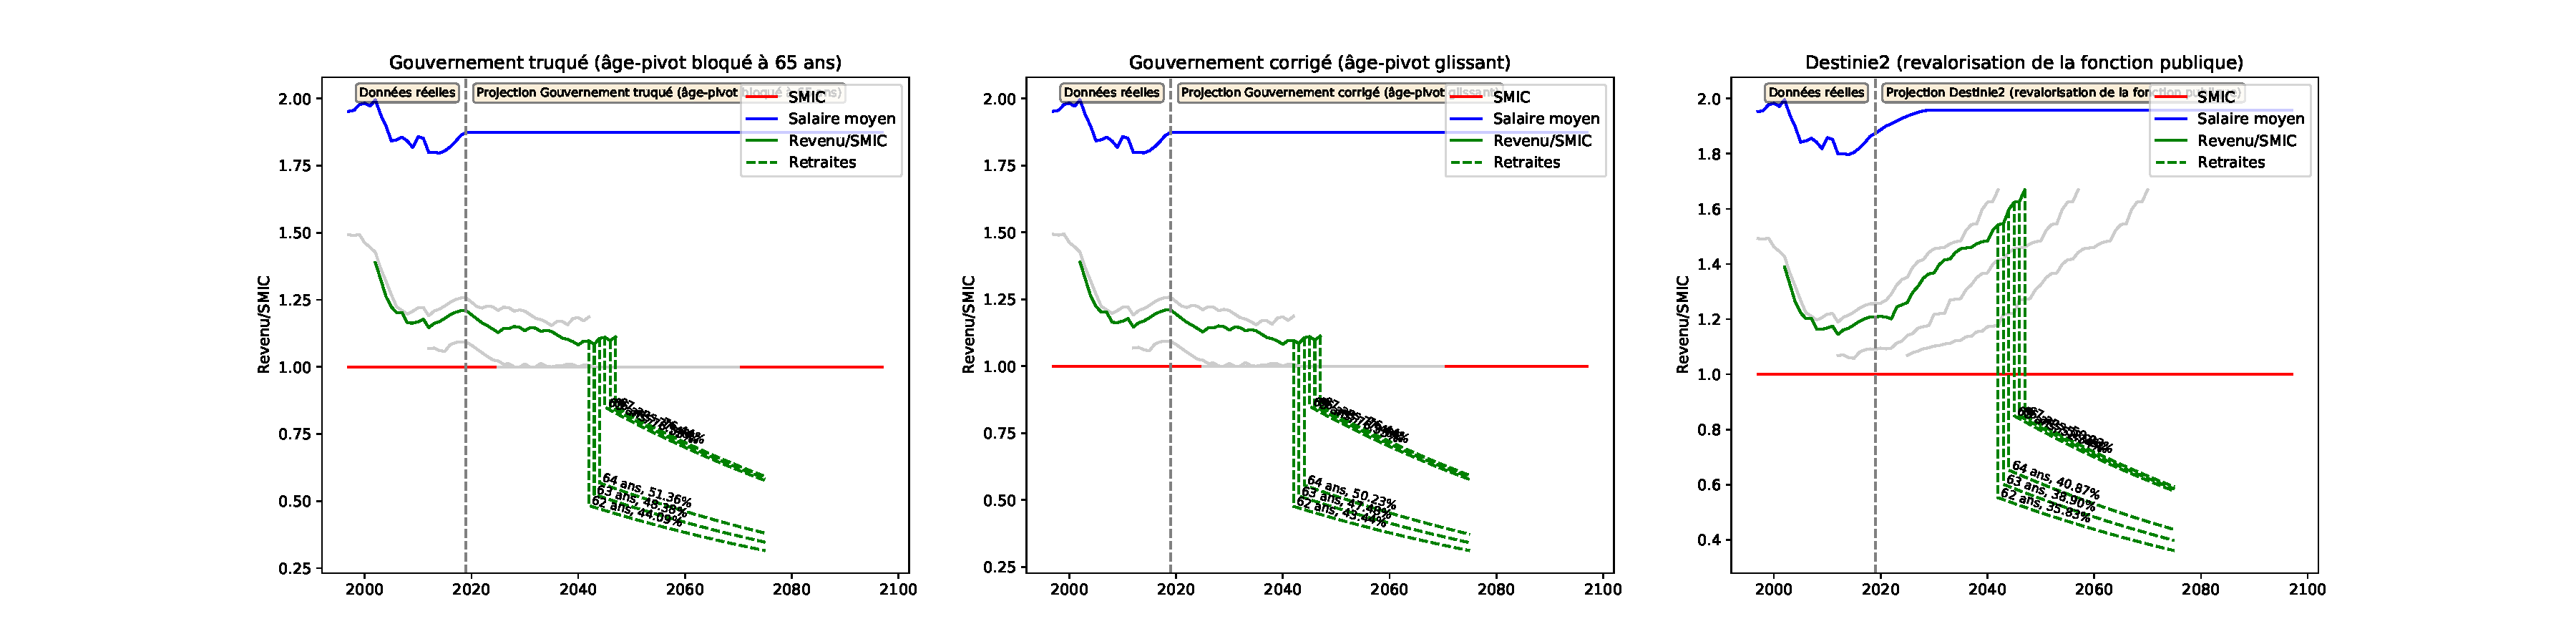
\includegraphics[width=0.9\textwidth]{fig/AdjTech_1980_22_dest_retraite.pdf}\end{center} \label{fig/AdjTech_1980_22_dest_retraite.pdf} 

\newpage 
 
\subsection{Génération 1990 (début en 2012)} 

\paragraph{Retraites possibles et ratios Revenu/SMIC à 70, 75, 80, 85, 90 ans avec le modèle \emph{Gouvernement truqué (âge-pivot bloqué à 65 ans)}}  
 
{ \scriptsize \begin{center} 
\begin{tabular}[htb]{|c|c||c|c||c|c||c||c|c|c|c|c|c|} 
\hline 
 Retraite en &  Âge &  Âge pivot &  Décote/Surcote &  Retraite (\euro{} 2019) &  Tx Rempl(\%) &  SMIC (\euro{} 2019) &  Retraite/SMIC &  Rev70/SMIC &  Rev75/SMIC &  Rev80/SMIC &  Rev85/SMIC &  Rev90/SMIC \\ 
\hline \hline 
 2052 &  62 &  65 ans 0 mois &  -15.00\% &  1181.65 &  {\bf 45.43} &  2601.14 &  {\bf {\color{red} 0.45}} &  {\bf {\color{red} 0.41}} &  {\bf {\color{red} 0.38}} &  {\bf {\color{red} 0.36}} &  {\bf {\color{red} 0.34}} &  {\bf {\color{red} 0.32}} \\ 
\hline 
 2053 &  63 &  65 ans 0 mois &  -10.00\% &  1300.43 &  {\bf 49.35} &  2634.96 &  {\bf {\color{red} 0.49}} &  {\bf {\color{red} 0.45}} &  {\bf {\color{red} 0.42}} &  {\bf {\color{red} 0.40}} &  {\bf {\color{red} 0.37}} &  {\bf {\color{red} 0.35}} \\ 
\hline 
 2054 &  64 &  65 ans 0 mois &  -5.00\% &  1425.82 &  {\bf 53.42} &  2669.21 &  {\bf {\color{red} 0.53}} &  {\bf {\color{red} 0.49}} &  {\bf {\color{red} 0.46}} &  {\bf {\color{red} 0.43}} &  {\bf {\color{red} 0.41}} &  {\bf {\color{red} 0.38}} \\ 
\hline 
 2055 &  65 &  65 ans 0 mois &  0.00\% &  2298.33 &  {\bf 85.00} &  2703.91 &  {\bf {\color{red} 0.85}} &  {\bf {\color{red} 0.80}} &  {\bf {\color{red} 0.75}} &  {\bf {\color{red} 0.70}} &  {\bf {\color{red} 0.66}} &  {\bf {\color{red} 0.62}} \\ 
\hline 
 2056 &  66 &  65 ans 0 mois &  5.00\% &  2328.20 &  {\bf 85.00} &  2739.06 &  {\bf {\color{red} 0.85}} &  {\bf {\color{red} 0.81}} &  {\bf {\color{red} 0.76}} &  {\bf {\color{red} 0.71}} &  {\bf {\color{red} 0.67}} &  {\bf {\color{red} 0.62}} \\ 
\hline 
 2057 &  67 &  65 ans 0 mois &  10.00\% &  2358.47 &  {\bf 85.00} &  2774.67 &  {\bf {\color{red} 0.85}} &  {\bf {\color{red} 0.82}} &  {\bf {\color{red} 0.77}} &  {\bf {\color{red} 0.72}} &  {\bf {\color{red} 0.67}} &  {\bf {\color{red} 0.63}} \\ 
\hline 
\hline 
\end{tabular} 
\end{center} } 
\paragraph{Retraites possibles et ratios Revenu/SMIC à 70, 75, 80, 85, 90 ans avec le modèle \emph{Gouvernement corrigé (âge-pivot glissant)}}  
 
{ \scriptsize \begin{center} 
\begin{tabular}[htb]{|c|c||c|c||c|c||c||c|c|c|c|c|c|} 
\hline 
 Retraite en &  Âge &  Âge pivot &  Décote/Surcote &  Retraite (\euro{} 2019) &  Tx Rempl(\%) &  SMIC (\euro{} 2019) &  Retraite/SMIC &  Rev70/SMIC &  Rev75/SMIC &  Rev80/SMIC &  Rev85/SMIC &  Rev90/SMIC \\ 
\hline \hline 
 2052 &  62 &  66 ans 1 mois &  -20.42\% &  1106.35 &  {\bf 42.53} &  2601.14 &  {\bf {\color{red} 0.43}} &  {\bf {\color{red} 0.38}} &  {\bf {\color{red} 0.36}} &  {\bf {\color{red} 0.34}} &  {\bf {\color{red} 0.32}} &  {\bf {\color{red} 0.30}} \\ 
\hline 
 2053 &  63 &  66 ans 2 mois &  -15.83\% &  1216.15 &  {\bf 46.15} &  2634.96 &  {\bf {\color{red} 0.46}} &  {\bf {\color{red} 0.42}} &  {\bf {\color{red} 0.40}} &  {\bf {\color{red} 0.37}} &  {\bf {\color{red} 0.35}} &  {\bf {\color{red} 0.33}} \\ 
\hline 
 2054 &  64 &  66 ans 3 mois &  -11.25\% &  1332.02 &  {\bf 49.90} &  2669.21 &  {\bf {\color{red} 0.50}} &  {\bf {\color{red} 0.46}} &  {\bf {\color{red} 0.43}} &  {\bf {\color{red} 0.41}} &  {\bf {\color{red} 0.38}} &  {\bf {\color{red} 0.36}} \\ 
\hline 
 2055 &  65 &  66 ans 4 mois &  -6.67\% &  2298.33 &  {\bf 85.00} &  2703.91 &  {\bf {\color{red} 0.85}} &  {\bf {\color{red} 0.80}} &  {\bf {\color{red} 0.75}} &  {\bf {\color{red} 0.70}} &  {\bf {\color{red} 0.66}} &  {\bf {\color{red} 0.62}} \\ 
\hline 
 2056 &  66 &  66 ans 5 mois &  -2.08\% &  2328.20 &  {\bf 85.00} &  2739.06 &  {\bf {\color{red} 0.85}} &  {\bf {\color{red} 0.81}} &  {\bf {\color{red} 0.76}} &  {\bf {\color{red} 0.71}} &  {\bf {\color{red} 0.67}} &  {\bf {\color{red} 0.62}} \\ 
\hline 
 2057 &  67 &  66 ans 6 mois &  2.50\% &  2358.47 &  {\bf 85.00} &  2774.67 &  {\bf {\color{red} 0.85}} &  {\bf {\color{red} 0.82}} &  {\bf {\color{red} 0.77}} &  {\bf {\color{red} 0.72}} &  {\bf {\color{red} 0.67}} &  {\bf {\color{red} 0.63}} \\ 
\hline 
\hline 
\end{tabular} 
\end{center} } 
\paragraph{Retraites possibles et ratios Revenu/SMIC à 70, 75, 80, 85, 90 ans avec le modèle \emph{Destinie2 (revalorisation de la fonction publique)}}  
 
{ \scriptsize \begin{center} 
\begin{tabular}[htb]{|c|c||c|c||c|c||c||c|c|c|c|c|c|} 
\hline 
 Retraite en &  Âge &  Âge pivot &  Décote/Surcote &  Retraite (\euro{} 2019) &  Tx Rempl(\%) &  SMIC (\euro{} 2019) &  Retraite/SMIC &  Rev70/SMIC &  Rev75/SMIC &  Rev80/SMIC &  Rev85/SMIC &  Rev90/SMIC \\ 
\hline \hline 
 2052 &  62 &  66 ans 1 mois &  -20.42\% &  1368.95 &  {\bf 36.07} &  2445.56 &  {\bf {\color{red} 0.56}} &  {\bf {\color{red} 0.50}} &  {\bf {\color{red} 0.47}} &  {\bf {\color{red} 0.44}} &  {\bf {\color{red} 0.42}} &  {\bf {\color{red} 0.39}} \\ 
\hline 
 2053 &  63 &  66 ans 2 mois &  -15.83\% &  1511.64 &  {\bf 39.32} &  2477.35 &  {\bf {\color{red} 0.61}} &  {\bf {\color{red} 0.56}} &  {\bf {\color{red} 0.52}} &  {\bf {\color{red} 0.49}} &  {\bf {\color{red} 0.46}} &  {\bf {\color{red} 0.43}} \\ 
\hline 
 2054 &  64 &  66 ans 3 mois &  -11.25\% &  1664.28 &  {\bf 41.45} &  2509.56 &  {\bf {\color{red} 0.66}} &  {\bf {\color{red} 0.61}} &  {\bf {\color{red} 0.58}} &  {\bf {\color{red} 0.54}} &  {\bf {\color{red} 0.51}} &  {\bf {\color{red} 0.47}} \\ 
\hline 
 2055 &  65 &  66 ans 4 mois &  -6.67\% &  2160.85 &  {\bf 52.34} &  2542.18 &  {\bf {\color{red} 0.85}} &  {\bf {\color{red} 0.80}} &  {\bf {\color{red} 0.75}} &  {\bf {\color{red} 0.70}} &  {\bf {\color{red} 0.66}} &  {\bf {\color{red} 0.62}} \\ 
\hline 
 2056 &  66 &  66 ans 5 mois &  -2.08\% &  2188.95 &  {\bf 52.34} &  2575.23 &  {\bf {\color{red} 0.85}} &  {\bf {\color{red} 0.81}} &  {\bf {\color{red} 0.76}} &  {\bf {\color{red} 0.71}} &  {\bf {\color{red} 0.67}} &  {\bf {\color{red} 0.62}} \\ 
\hline 
 2057 &  67 &  66 ans 6 mois &  2.50\% &  2217.40 &  {\bf 51.13} &  2608.71 &  {\bf {\color{red} 0.85}} &  {\bf {\color{red} 0.82}} &  {\bf {\color{red} 0.77}} &  {\bf {\color{red} 0.72}} &  {\bf {\color{red} 0.67}} &  {\bf {\color{red} 0.63}} \\ 
\hline 
\hline 
\end{tabular} 
\end{center} } 

 \begin{center}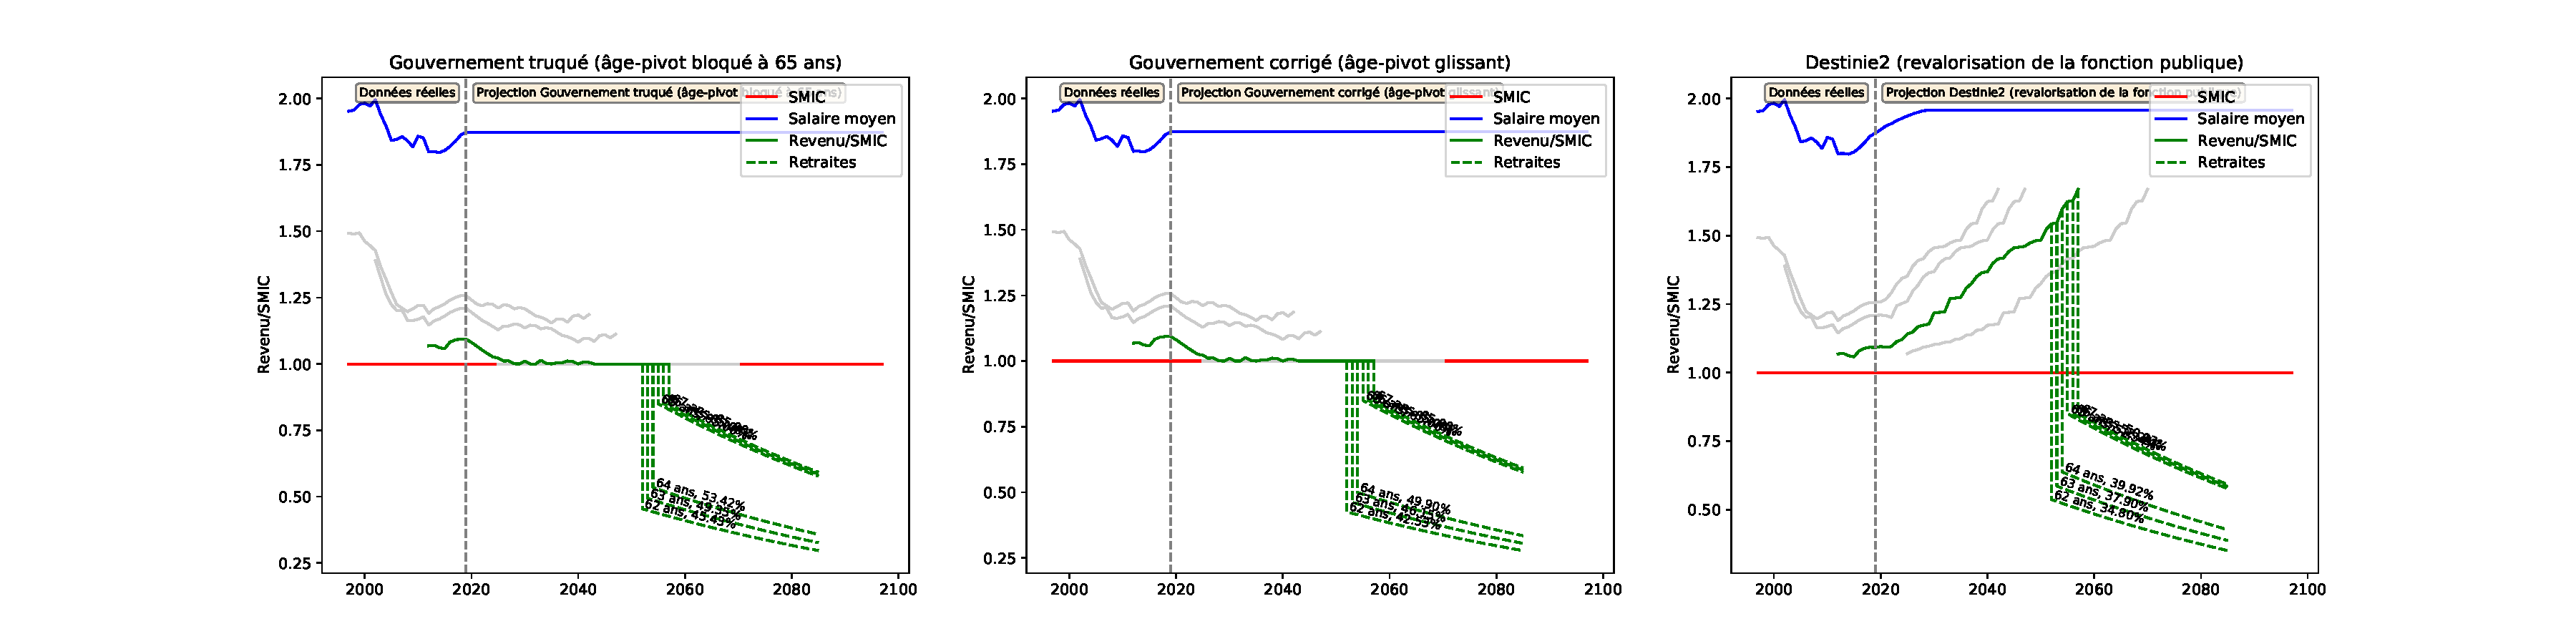
\includegraphics[width=0.9\textwidth]{fig/AdjTech_1990_22_dest_retraite.pdf}\end{center} \label{fig/AdjTech_1990_22_dest_retraite.pdf} 

\newpage 
 
\subsection{Génération 2003 (début en 2025)} 

\paragraph{Retraites possibles et ratios Revenu/SMIC à 70, 75, 80, 85, 90 ans avec le modèle \emph{Gouvernement truqué (âge-pivot bloqué à 65 ans)}}  
 
{ \scriptsize \begin{center} 
\begin{tabular}[htb]{|c|c||c|c||c|c||c||c|c|c|c|c|c|} 
\hline 
 Retraite en &  Âge &  Âge pivot &  Décote/Surcote &  Retraite (\euro{} 2019) &  Tx Rempl(\%) &  SMIC (\euro{} 2019) &  Retraite/SMIC &  Rev70/SMIC &  Rev75/SMIC &  Rev80/SMIC &  Rev85/SMIC &  Rev90/SMIC \\ 
\hline \hline 
 2065 &  62 &  65 ans 0 mois &  -15.00\% &  1457.41 &  {\bf 47.37} &  3076.71 &  {\bf {\color{red} 0.47}} &  {\bf {\color{red} 0.43}} &  {\bf {\color{red} 0.40}} &  {\bf {\color{red} 0.38}} &  {\bf {\color{red} 0.35}} &  {\bf {\color{red} 0.33}} \\ 
\hline 
 2066 &  63 &  65 ans 0 mois &  -10.00\% &  1602.25 &  {\bf 51.41} &  3116.71 &  {\bf {\color{red} 0.51}} &  {\bf {\color{red} 0.47}} &  {\bf {\color{red} 0.44}} &  {\bf {\color{red} 0.41}} &  {\bf {\color{red} 0.39}} &  {\bf {\color{red} 0.36}} \\ 
\hline 
 2067 &  64 &  65 ans 0 mois &  -5.00\% &  1755.00 &  {\bf 55.59} &  3157.23 &  {\bf {\color{red} 0.56}} &  {\bf {\color{red} 0.51}} &  {\bf {\color{red} 0.48}} &  {\bf {\color{red} 0.45}} &  {\bf {\color{red} 0.42}} &  {\bf {\color{red} 0.40}} \\ 
\hline 
 2068 &  65 &  65 ans 0 mois &  0.00\% &  2718.53 &  {\bf 85.00} &  3198.27 &  {\bf {\color{red} 0.85}} &  {\bf {\color{red} 0.80}} &  {\bf {\color{red} 0.75}} &  {\bf {\color{red} 0.70}} &  {\bf {\color{red} 0.66}} &  {\bf {\color{red} 0.62}} \\ 
\hline 
 2069 &  66 &  65 ans 0 mois &  5.00\% &  2753.87 &  {\bf 85.00} &  3239.85 &  {\bf {\color{red} 0.85}} &  {\bf {\color{red} 0.81}} &  {\bf {\color{red} 0.76}} &  {\bf {\color{red} 0.71}} &  {\bf {\color{red} 0.67}} &  {\bf {\color{red} 0.62}} \\ 
\hline 
 2070 &  67 &  65 ans 0 mois &  10.00\% &  2789.67 &  {\bf 85.00} &  3281.97 &  {\bf {\color{red} 0.85}} &  {\bf {\color{red} 0.82}} &  {\bf {\color{red} 0.77}} &  {\bf {\color{red} 0.72}} &  {\bf {\color{red} 0.67}} &  {\bf {\color{red} 0.63}} \\ 
\hline 
\hline 
\end{tabular} 
\end{center} } 
\paragraph{Retraites possibles et ratios Revenu/SMIC à 70, 75, 80, 85, 90 ans avec le modèle \emph{Gouvernement corrigé (âge-pivot glissant)}}  
 
{ \scriptsize \begin{center} 
\begin{tabular}[htb]{|c|c||c|c||c|c||c||c|c|c|c|c|c|} 
\hline 
 Retraite en &  Âge &  Âge pivot &  Décote/Surcote &  Retraite (\euro{} 2019) &  Tx Rempl(\%) &  SMIC (\euro{} 2019) &  Retraite/SMIC &  Rev70/SMIC &  Rev75/SMIC &  Rev80/SMIC &  Rev85/SMIC &  Rev90/SMIC \\ 
\hline \hline 
 2065 &  62 &  67 ans 2 mois &  -25.83\% &  1271.67 &  {\bf 41.33} &  3076.71 &  {\bf {\color{red} 0.41}} &  {\bf {\color{red} 0.37}} &  {\bf {\color{red} 0.35}} &  {\bf {\color{red} 0.33}} &  {\bf {\color{red} 0.31}} &  {\bf {\color{red} 0.29}} \\ 
\hline 
 2066 &  63 &  67 ans 3 mois &  -21.25\% &  1401.97 &  {\bf 44.98} &  3116.71 &  {\bf {\color{red} 0.45}} &  {\bf {\color{red} 0.41}} &  {\bf {\color{red} 0.39}} &  {\bf {\color{red} 0.36}} &  {\bf {\color{red} 0.34}} &  {\bf {\color{red} 0.32}} \\ 
\hline 
 2067 &  64 &  67 ans 4 mois &  -16.67\% &  1539.47 &  {\bf 48.76} &  3157.23 &  {\bf {\color{red} 0.49}} &  {\bf {\color{red} 0.45}} &  {\bf {\color{red} 0.42}} &  {\bf {\color{red} 0.40}} &  {\bf {\color{red} 0.37}} &  {\bf {\color{red} 0.35}} \\ 
\hline 
 2068 &  65 &  67 ans 5 mois &  -12.08\% &  2718.53 &  {\bf 85.00} &  3198.27 &  {\bf {\color{red} 0.85}} &  {\bf {\color{red} 0.80}} &  {\bf {\color{red} 0.75}} &  {\bf {\color{red} 0.70}} &  {\bf {\color{red} 0.66}} &  {\bf {\color{red} 0.62}} \\ 
\hline 
 2069 &  66 &  67 ans 6 mois &  -7.50\% &  2753.87 &  {\bf 85.00} &  3239.85 &  {\bf {\color{red} 0.85}} &  {\bf {\color{red} 0.81}} &  {\bf {\color{red} 0.76}} &  {\bf {\color{red} 0.71}} &  {\bf {\color{red} 0.67}} &  {\bf {\color{red} 0.62}} \\ 
\hline 
 2070 &  67 &  67 ans 7 mois &  -2.92\% &  2789.67 &  {\bf 85.00} &  3281.97 &  {\bf {\color{red} 0.85}} &  {\bf {\color{red} 0.82}} &  {\bf {\color{red} 0.77}} &  {\bf {\color{red} 0.72}} &  {\bf {\color{red} 0.67}} &  {\bf {\color{red} 0.63}} \\ 
\hline 
\hline 
\end{tabular} 
\end{center} } 
\paragraph{Retraites possibles et ratios Revenu/SMIC à 70, 75, 80, 85, 90 ans avec le modèle \emph{Destinie2 (revalorisation de la fonction publique)}}  
 
{ \scriptsize \begin{center} 
\begin{tabular}[htb]{|c|c||c|c||c|c||c||c|c|c|c|c|c|} 
\hline 
 Retraite en &  Âge &  Âge pivot &  Décote/Surcote &  Retraite (\euro{} 2019) &  Tx Rempl(\%) &  SMIC (\euro{} 2019) &  Retraite/SMIC &  Rev70/SMIC &  Rev75/SMIC &  Rev80/SMIC &  Rev85/SMIC &  Rev90/SMIC \\ 
\hline \hline 
 2065 &  62 &  67 ans 2 mois &  -25.83\% &  1584.92 &  {\bf 35.31} &  2892.68 &  {\bf {\color{red} 0.55}} &  {\bf {\color{red} 0.49}} &  {\bf {\color{red} 0.46}} &  {\bf {\color{red} 0.43}} &  {\bf {\color{red} 0.41}} &  {\bf {\color{red} 0.38}} \\ 
\hline 
 2066 &  63 &  67 ans 3 mois &  -21.25\% &  1754.58 &  {\bf 38.59} &  2930.29 &  {\bf {\color{red} 0.60}} &  {\bf {\color{red} 0.55}} &  {\bf {\color{red} 0.51}} &  {\bf {\color{red} 0.48}} &  {\bf {\color{red} 0.45}} &  {\bf {\color{red} 0.42}} \\ 
\hline 
 2067 &  64 &  67 ans 4 mois &  -16.67\% &  1935.93 &  {\bf 40.76} &  2968.38 &  {\bf {\color{red} 0.65}} &  {\bf {\color{red} 0.60}} &  {\bf {\color{red} 0.57}} &  {\bf {\color{red} 0.53}} &  {\bf {\color{red} 0.50}} &  {\bf {\color{red} 0.47}} \\ 
\hline 
 2068 &  65 &  67 ans 5 mois &  -12.08\% &  2555.93 &  {\bf 52.34} &  3006.97 &  {\bf {\color{red} 0.85}} &  {\bf {\color{red} 0.80}} &  {\bf {\color{red} 0.75}} &  {\bf {\color{red} 0.70}} &  {\bf {\color{red} 0.66}} &  {\bf {\color{red} 0.62}} \\ 
\hline 
 2069 &  66 &  67 ans 6 mois &  -7.50\% &  2589.15 &  {\bf 52.34} &  3046.06 &  {\bf {\color{red} 0.85}} &  {\bf {\color{red} 0.81}} &  {\bf {\color{red} 0.76}} &  {\bf {\color{red} 0.71}} &  {\bf {\color{red} 0.67}} &  {\bf {\color{red} 0.62}} \\ 
\hline 
 2070 &  67 &  67 ans 7 mois &  -2.92\% &  2622.81 &  {\bf 51.13} &  3085.66 &  {\bf {\color{red} 0.85}} &  {\bf {\color{red} 0.82}} &  {\bf {\color{red} 0.77}} &  {\bf {\color{red} 0.72}} &  {\bf {\color{red} 0.67}} &  {\bf {\color{red} 0.63}} \\ 
\hline 
\hline 
\end{tabular} 
\end{center} } 

 \begin{center}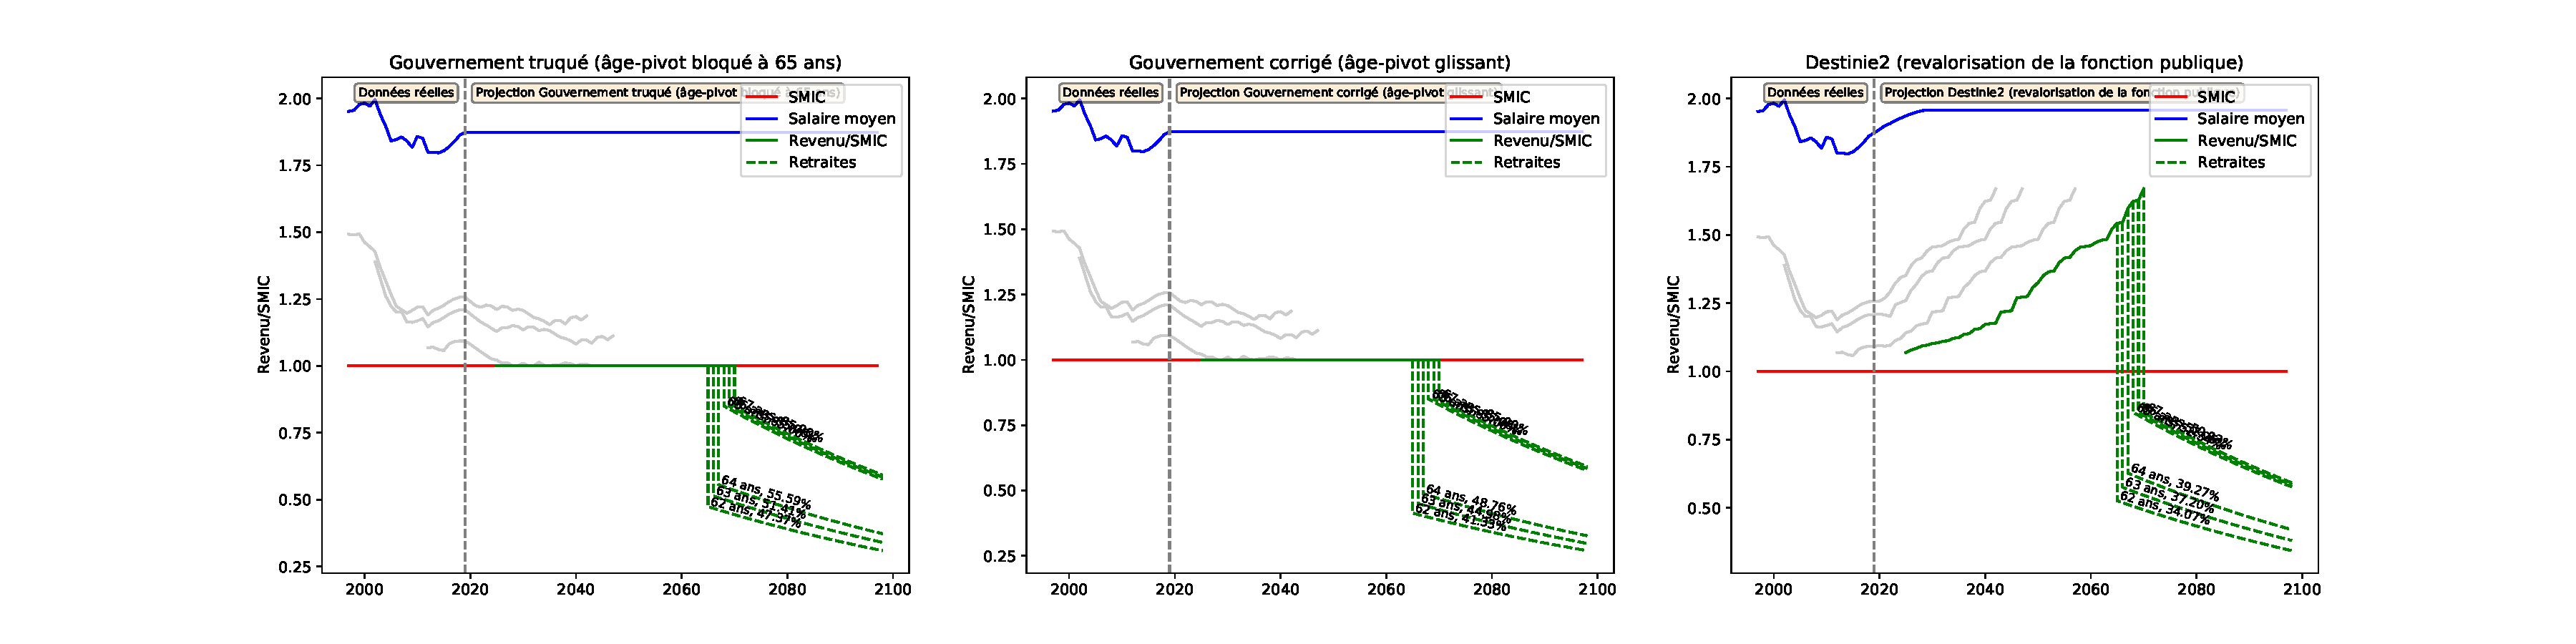
\includegraphics[width=0.9\textwidth]{fig/AdjTech_2003_22_dest_retraite.pdf}\end{center} \label{fig/AdjTech_2003_22_dest_retraite.pdf} 

\newpage 
 
\chapter{Rédacteur territorial (C2 puis C1)} 

\begin{minipage}{0.55\linewidth}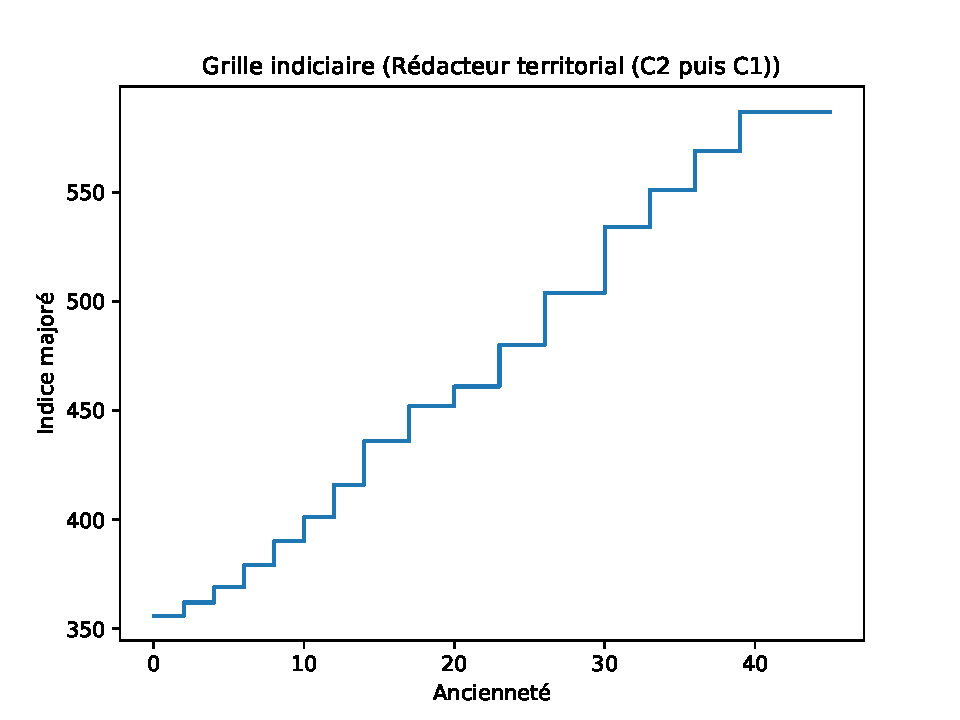
\includegraphics[width=0.7\textwidth]{fig/grille_Redacteur.pdf}\end{minipage} 
\begin{minipage}{0.3\linewidth} 
 \begin{center} 

\begin{tabular}[htb]{|c|c|} 
\hline 
 Indice majoré &  Durée (années) \\ 
\hline \hline 
 356 &  2.00 \\ 
\hline 
 362 &  2.00 \\ 
\hline 
 369 &  2.00 \\ 
\hline 
 379 &  2.00 \\ 
\hline 
 390 &  2.00 \\ 
\hline 
 401 &  2.00 \\ 
\hline 
 416 &  2.00 \\ 
\hline 
 436 &  3.00 \\ 
\hline 
 452 &  3.00 \\ 
\hline 
 461 &  3.00 \\ 
\hline 
 480 &  3.00 \\ 
\hline 
 504 &  4.00 \\ 
\hline 
 534 &  3.00 \\ 
\hline 
 551 &  3.00 \\ 
\hline 
 569 &  3.00 \\ 
\hline 
 587 &   \\ 
\hline 
\hline 
\end{tabular} 
\end{center} 
 \end{minipage} 


 \addto{\captionsenglish}{ \renewcommand{\mtctitle}{}} \setcounter{minitocdepth}{2} 
 \minitoc \newpage 

\section{Début de carrière à 22 ans} 

\subsection{Génération 1975 (début en 1997)} 

\paragraph{Retraites possibles et ratios Revenu/SMIC à 70, 75, 80, 85, 90 ans avec le modèle \emph{Gouvernement truqué (âge-pivot bloqué à 65 ans)}}  
 
{ \scriptsize \begin{center} 
\begin{tabular}[htb]{|c|c||c|c||c|c||c||c|c|c|c|c|c|} 
\hline 
 Retraite en &  Âge &  Âge pivot &  Décote/Surcote &  Retraite (\euro{} 2019) &  Tx Rempl(\%) &  SMIC (\euro{} 2019) &  Retraite/SMIC &  Rev70/SMIC &  Rev75/SMIC &  Rev80/SMIC &  Rev85/SMIC &  Rev90/SMIC \\ 
\hline \hline 
 2037 &  62 &  64 ans 10 mois &  -14.17\% &  1430.63 &  {\bf 39.90} &  2143.00 &  {\bf {\color{red} 0.67}} &  {\bf {\color{red} 0.60}} &  {\bf {\color{red} 0.56}} &  {\bf {\color{red} 0.53}} &  {\bf {\color{red} 0.50}} &  {\bf {\color{red} 0.46}} \\ 
\hline 
 2038 &  63 &  64 ans 11 mois &  -9.58\% &  1563.72 &  {\bf 43.53} &  2170.86 &  {\bf {\color{red} 0.72}} &  {\bf {\color{red} 0.66}} &  {\bf {\color{red} 0.62}} &  {\bf {\color{red} 0.58}} &  {\bf {\color{red} 0.54}} &  {\bf {\color{red} 0.51}} \\ 
\hline 
 2039 &  64 &  65 ans 0 mois &  -5.00\% &  1704.37 &  {\bf 47.36} &  2199.08 &  {\bf {\color{red} 0.78}} &  {\bf {\color{red} 0.72}} &  {\bf {\color{red} 0.67}} &  {\bf {\color{red} 0.63}} &  {\bf {\color{red} 0.59}} &  {\bf {\color{red} 0.55}} \\ 
\hline 
 2040 &  65 &  65 ans 0 mois &  0.00\% &  1893.52 &  {\bf 52.52} &  2227.67 &  {\bf {\color{red} 0.85}} &  {\bf {\color{red} 0.80}} &  {\bf {\color{red} 0.75}} &  {\bf {\color{red} 0.70}} &  {\bf {\color{red} 0.66}} &  {\bf {\color{red} 0.62}} \\ 
\hline 
 2041 &  66 &  65 ans 0 mois &  5.00\% &  2025.90 &  {\bf 56.09} &  2256.63 &  {\bf {\color{red} 0.90}} &  {\bf {\color{red} 0.85}} &  {\bf {\color{red} 0.80}} &  {\bf {\color{red} 0.75}} &  {\bf {\color{red} 0.70}} &  {\bf {\color{red} 0.66}} \\ 
\hline 
 2042 &  67 &  65 ans 0 mois &  10.00\% &  2200.46 &  {\bf 60.82} &  2285.97 &  {\bf {\color{red} 0.96}} &  {\bf {\color{red} 0.93}} &  {\bf {\color{red} 0.87}} &  {\bf {\color{red} 0.81}} &  {\bf {\color{red} 0.76}} &  {\bf {\color{red} 0.72}} \\ 
\hline 
\hline 
\end{tabular} 
\end{center} } 
\paragraph{Retraites possibles et ratios Revenu/SMIC à 70, 75, 80, 85, 90 ans avec le modèle \emph{Gouvernement corrigé (âge-pivot glissant)}}  
 
{ \scriptsize \begin{center} 
\begin{tabular}[htb]{|c|c||c|c||c|c||c||c|c|c|c|c|c|} 
\hline 
 Retraite en &  Âge &  Âge pivot &  Décote/Surcote &  Retraite (\euro{} 2019) &  Tx Rempl(\%) &  SMIC (\euro{} 2019) &  Retraite/SMIC &  Rev70/SMIC &  Rev75/SMIC &  Rev80/SMIC &  Rev85/SMIC &  Rev90/SMIC \\ 
\hline \hline 
 2037 &  62 &  64 ans 10 mois &  -14.17\% &  1430.63 &  {\bf 39.90} &  2143.00 &  {\bf {\color{red} 0.67}} &  {\bf {\color{red} 0.60}} &  {\bf {\color{red} 0.56}} &  {\bf {\color{red} 0.53}} &  {\bf {\color{red} 0.50}} &  {\bf {\color{red} 0.46}} \\ 
\hline 
 2038 &  63 &  64 ans 11 mois &  -9.58\% &  1563.72 &  {\bf 43.53} &  2170.86 &  {\bf {\color{red} 0.72}} &  {\bf {\color{red} 0.66}} &  {\bf {\color{red} 0.62}} &  {\bf {\color{red} 0.58}} &  {\bf {\color{red} 0.54}} &  {\bf {\color{red} 0.51}} \\ 
\hline 
 2039 &  64 &  65 ans 0 mois &  -5.00\% &  1704.37 &  {\bf 47.36} &  2199.08 &  {\bf {\color{red} 0.78}} &  {\bf {\color{red} 0.72}} &  {\bf {\color{red} 0.67}} &  {\bf {\color{red} 0.63}} &  {\bf {\color{red} 0.59}} &  {\bf {\color{red} 0.55}} \\ 
\hline 
 2040 &  65 &  65 ans 1 mois &  -0.42\% &  1893.52 &  {\bf 52.52} &  2227.67 &  {\bf {\color{red} 0.85}} &  {\bf {\color{red} 0.80}} &  {\bf {\color{red} 0.75}} &  {\bf {\color{red} 0.70}} &  {\bf {\color{red} 0.66}} &  {\bf {\color{red} 0.62}} \\ 
\hline 
 2041 &  66 &  65 ans 2 mois &  4.17\% &  2009.82 &  {\bf 55.65} &  2256.63 &  {\bf {\color{red} 0.89}} &  {\bf {\color{red} 0.85}} &  {\bf {\color{red} 0.79}} &  {\bf {\color{red} 0.74}} &  {\bf {\color{red} 0.70}} &  {\bf {\color{red} 0.65}} \\ 
\hline 
 2042 &  67 &  65 ans 3 mois &  8.75\% &  2175.46 &  {\bf 60.13} &  2285.97 &  {\bf {\color{red} 0.95}} &  {\bf {\color{red} 0.92}} &  {\bf {\color{red} 0.86}} &  {\bf {\color{red} 0.80}} &  {\bf {\color{red} 0.75}} &  {\bf {\color{red} 0.71}} \\ 
\hline 
\hline 
\end{tabular} 
\end{center} } 
\paragraph{Retraites possibles et ratios Revenu/SMIC à 70, 75, 80, 85, 90 ans avec le modèle \emph{Destinie2 (revalorisation de la fonction publique)}}  
 
{ \scriptsize \begin{center} 
\begin{tabular}[htb]{|c|c||c|c||c|c||c||c|c|c|c|c|c|} 
\hline 
 Retraite en &  Âge &  Âge pivot &  Décote/Surcote &  Retraite (\euro{} 2019) &  Tx Rempl(\%) &  SMIC (\euro{} 2019) &  Retraite/SMIC &  Rev70/SMIC &  Rev75/SMIC &  Rev80/SMIC &  Rev85/SMIC &  Rev90/SMIC \\ 
\hline \hline 
 2037 &  62 &  64 ans 10 mois &  -14.17\% &  1577.19 &  {\bf 35.28} &  2014.82 &  {\bf {\color{red} 0.78}} &  {\bf {\color{red} 0.71}} &  {\bf {\color{red} 0.66}} &  {\bf {\color{red} 0.62}} &  {\bf {\color{red} 0.58}} &  {\bf {\color{red} 0.55}} \\ 
\hline 
 2038 &  63 &  64 ans 11 mois &  -9.58\% &  1731.07 &  {\bf 38.23} &  2041.01 &  {\bf {\color{red} 0.85}} &  {\bf {\color{red} 0.77}} &  {\bf {\color{red} 0.73}} &  {\bf {\color{red} 0.68}} &  {\bf {\color{red} 0.64}} &  {\bf {\color{red} 0.60}} \\ 
\hline 
 2039 &  64 &  65 ans 0 mois &  -5.00\% &  1894.75 &  {\bf 41.30} &  2067.55 &  {\bf {\color{red} 0.92}} &  {\bf {\color{red} 0.85}} &  {\bf {\color{red} 0.80}} &  {\bf {\color{red} 0.75}} &  {\bf {\color{red} 0.70}} &  {\bf {\color{red} 0.66}} \\ 
\hline 
 2040 &  65 &  65 ans 1 mois &  -0.42\% &  2068.76 &  {\bf 44.52} &  2094.43 &  {\bf {\color{red} 0.99}} &  {\bf {\color{red} 0.93}} &  {\bf {\color{red} 0.87}} &  {\bf {\color{red} 0.81}} &  {\bf {\color{red} 0.76}} &  {\bf {\color{red} 0.72}} \\ 
\hline 
 2041 &  66 &  65 ans 2 mois &  4.17\% &  2253.71 &  {\bf 47.88} &  2121.65 &  {\bf 1.06} &  {\bf 1.01} &  {\bf {\color{red} 0.95}} &  {\bf {\color{red} 0.89}} &  {\bf {\color{red} 0.83}} &  {\bf {\color{red} 0.78}} \\ 
\hline 
 2042 &  67 &  65 ans 3 mois &  8.75\% &  2450.22 &  {\bf 51.38} &  2149.23 &  {\bf 1.14} &  {\bf 1.10} &  {\bf 1.03} &  {\bf {\color{red} 0.96}} &  {\bf {\color{red} 0.90}} &  {\bf {\color{red} 0.85}} \\ 
\hline 
\hline 
\end{tabular} 
\end{center} } 

 \begin{center}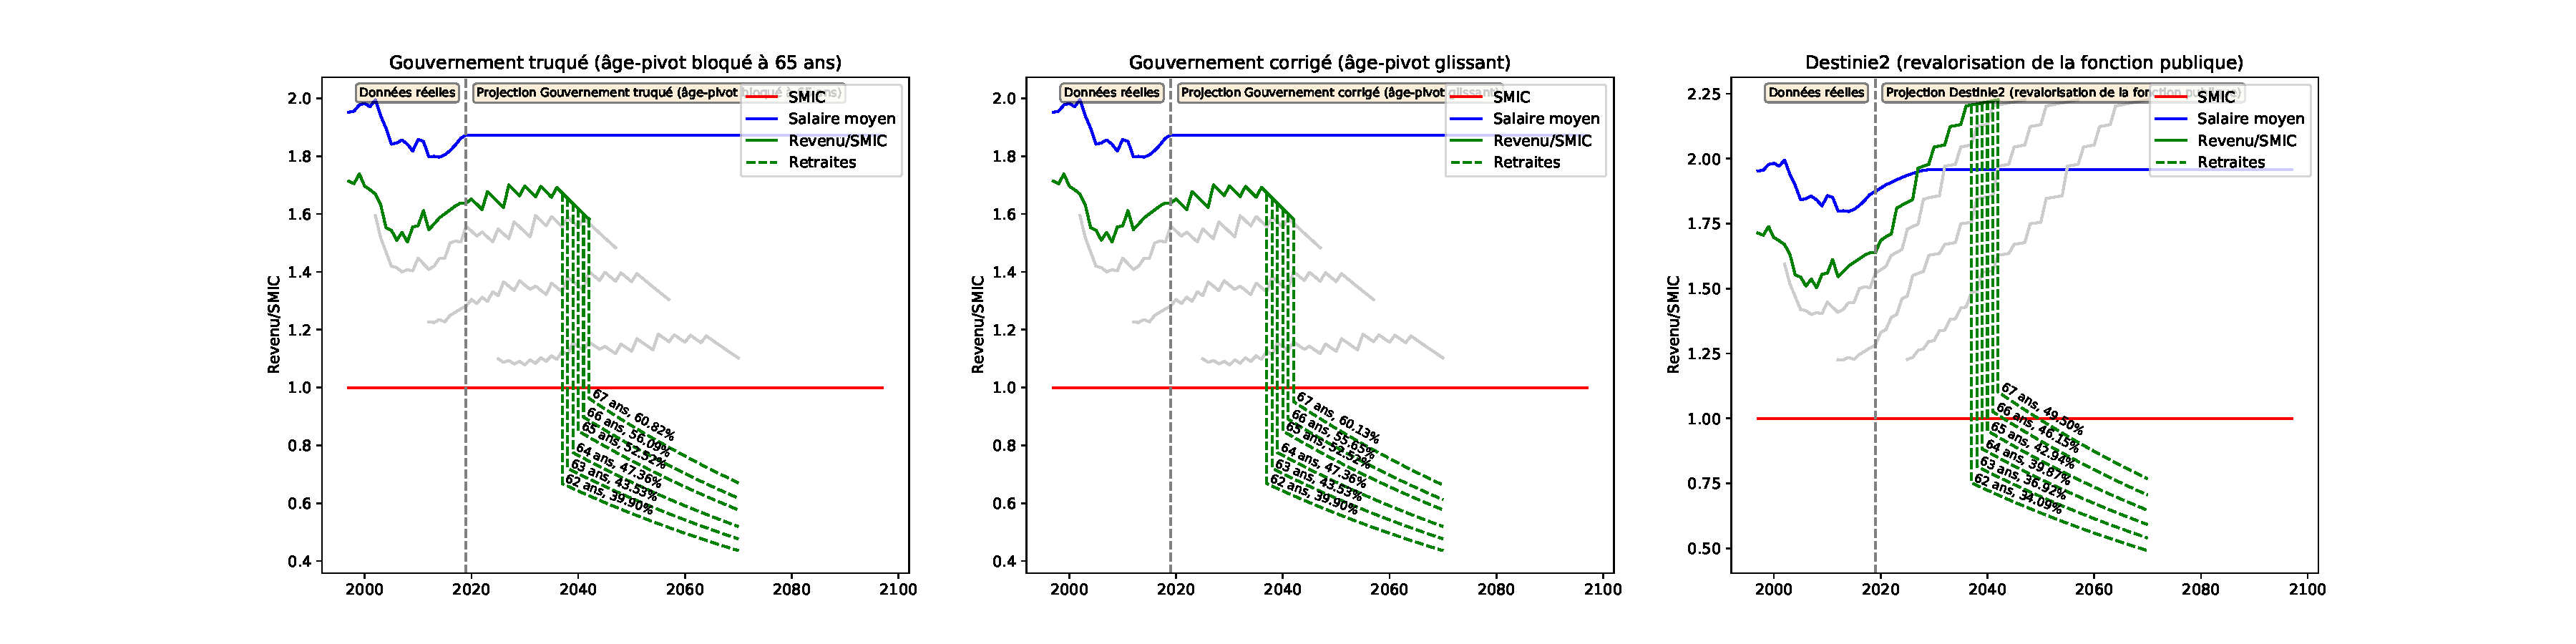
\includegraphics[width=0.9\textwidth]{fig/Redacteur_1975_22_dest_retraite.pdf}\end{center} \label{fig/Redacteur_1975_22_dest_retraite.pdf} 

\newpage 
 
\subsection{Génération 1980 (début en 2002)} 

\paragraph{Retraites possibles et ratios Revenu/SMIC à 70, 75, 80, 85, 90 ans avec le modèle \emph{Gouvernement truqué (âge-pivot bloqué à 65 ans)}}  
 
{ \scriptsize \begin{center} 
\begin{tabular}[htb]{|c|c||c|c||c|c||c||c|c|c|c|c|c|} 
\hline 
 Retraite en &  Âge &  Âge pivot &  Décote/Surcote &  Retraite (\euro{} 2019) &  Tx Rempl(\%) &  SMIC (\euro{} 2019) &  Retraite/SMIC &  Rev70/SMIC &  Rev75/SMIC &  Rev80/SMIC &  Rev85/SMIC &  Rev90/SMIC \\ 
\hline \hline 
 2042 &  62 &  65 ans 0 mois &  -15.00\% &  1443.92 &  {\bf 40.27} &  2285.97 &  {\bf {\color{red} 0.63}} &  {\bf {\color{red} 0.57}} &  {\bf {\color{red} 0.53}} &  {\bf {\color{red} 0.50}} &  {\bf {\color{red} 0.47}} &  {\bf {\color{red} 0.44}} \\ 
\hline 
 2043 &  63 &  65 ans 0 mois &  -10.00\% &  1591.38 &  {\bf 44.30} &  2315.68 &  {\bf {\color{red} 0.69}} &  {\bf {\color{red} 0.63}} &  {\bf {\color{red} 0.59}} &  {\bf {\color{red} 0.55}} &  {\bf {\color{red} 0.52}} &  {\bf {\color{red} 0.48}} \\ 
\hline 
 2044 &  64 &  65 ans 0 mois &  -5.00\% &  1747.92 &  {\bf 48.57} &  2345.79 &  {\bf {\color{red} 0.75}} &  {\bf {\color{red} 0.69}} &  {\bf {\color{red} 0.65}} &  {\bf {\color{red} 0.61}} &  {\bf {\color{red} 0.57}} &  {\bf {\color{red} 0.53}} \\ 
\hline 
 2045 &  65 &  65 ans 0 mois &  0.00\% &  2019.84 &  {\bf 56.03} &  2376.28 &  {\bf {\color{red} 0.85}} &  {\bf {\color{red} 0.80}} &  {\bf {\color{red} 0.75}} &  {\bf {\color{red} 0.70}} &  {\bf {\color{red} 0.66}} &  {\bf {\color{red} 0.62}} \\ 
\hline 
 2046 &  66 &  65 ans 0 mois &  5.00\% &  2088.63 &  {\bf 57.83} &  2407.18 &  {\bf {\color{red} 0.87}} &  {\bf {\color{red} 0.82}} &  {\bf {\color{red} 0.77}} &  {\bf {\color{red} 0.72}} &  {\bf {\color{red} 0.68}} &  {\bf {\color{red} 0.64}} \\ 
\hline 
 2047 &  67 &  65 ans 0 mois &  10.00\% &  2271.93 &  {\bf 62.79} &  2438.47 &  {\bf {\color{red} 0.93}} &  {\bf {\color{red} 0.90}} &  {\bf {\color{red} 0.84}} &  {\bf {\color{red} 0.79}} &  {\bf {\color{red} 0.74}} &  {\bf {\color{red} 0.69}} \\ 
\hline 
\hline 
\end{tabular} 
\end{center} } 
\paragraph{Retraites possibles et ratios Revenu/SMIC à 70, 75, 80, 85, 90 ans avec le modèle \emph{Gouvernement corrigé (âge-pivot glissant)}}  
 
{ \scriptsize \begin{center} 
\begin{tabular}[htb]{|c|c||c|c||c|c||c||c|c|c|c|c|c|} 
\hline 
 Retraite en &  Âge &  Âge pivot &  Décote/Surcote &  Retraite (\euro{} 2019) &  Tx Rempl(\%) &  SMIC (\euro{} 2019) &  Retraite/SMIC &  Rev70/SMIC &  Rev75/SMIC &  Rev80/SMIC &  Rev85/SMIC &  Rev90/SMIC \\ 
\hline \hline 
 2042 &  62 &  65 ans 3 mois &  -16.25\% &  1422.69 &  {\bf 39.68} &  2285.97 &  {\bf {\color{red} 0.62}} &  {\bf {\color{red} 0.56}} &  {\bf {\color{red} 0.53}} &  {\bf {\color{red} 0.49}} &  {\bf {\color{red} 0.46}} &  {\bf {\color{red} 0.43}} \\ 
\hline 
 2043 &  63 &  65 ans 4 mois &  -11.67\% &  1561.91 &  {\bf 43.48} &  2315.68 &  {\bf {\color{red} 0.67}} &  {\bf {\color{red} 0.62}} &  {\bf {\color{red} 0.58}} &  {\bf {\color{red} 0.54}} &  {\bf {\color{red} 0.51}} &  {\bf {\color{red} 0.48}} \\ 
\hline 
 2044 &  64 &  65 ans 5 mois &  -7.08\% &  1709.59 &  {\bf 47.51} &  2345.79 &  {\bf {\color{red} 0.73}} &  {\bf {\color{red} 0.67}} &  {\bf {\color{red} 0.63}} &  {\bf {\color{red} 0.59}} &  {\bf {\color{red} 0.56}} &  {\bf {\color{red} 0.52}} \\ 
\hline 
 2045 &  65 &  65 ans 6 mois &  -2.50\% &  2019.84 &  {\bf 56.03} &  2376.28 &  {\bf {\color{red} 0.85}} &  {\bf {\color{red} 0.80}} &  {\bf {\color{red} 0.75}} &  {\bf {\color{red} 0.70}} &  {\bf {\color{red} 0.66}} &  {\bf {\color{red} 0.62}} \\ 
\hline 
 2046 &  66 &  65 ans 7 mois &  2.08\% &  2046.10 &  {\bf 56.65} &  2407.18 &  {\bf {\color{red} 0.85}} &  {\bf {\color{red} 0.81}} &  {\bf {\color{red} 0.76}} &  {\bf {\color{red} 0.71}} &  {\bf {\color{red} 0.67}} &  {\bf {\color{red} 0.62}} \\ 
\hline 
 2047 &  67 &  65 ans 8 mois &  6.67\% &  2203.09 &  {\bf 60.89} &  2438.47 &  {\bf {\color{red} 0.90}} &  {\bf {\color{red} 0.87}} &  {\bf {\color{red} 0.81}} &  {\bf {\color{red} 0.76}} &  {\bf {\color{red} 0.72}} &  {\bf {\color{red} 0.67}} \\ 
\hline 
\hline 
\end{tabular} 
\end{center} } 
\paragraph{Retraites possibles et ratios Revenu/SMIC à 70, 75, 80, 85, 90 ans avec le modèle \emph{Destinie2 (revalorisation de la fonction publique)}}  
 
{ \scriptsize \begin{center} 
\begin{tabular}[htb]{|c|c||c|c||c|c||c||c|c|c|c|c|c|} 
\hline 
 Retraite en &  Âge &  Âge pivot &  Décote/Surcote &  Retraite (\euro{} 2019) &  Tx Rempl(\%) &  SMIC (\euro{} 2019) &  Retraite/SMIC &  Rev70/SMIC &  Rev75/SMIC &  Rev80/SMIC &  Rev85/SMIC &  Rev90/SMIC \\ 
\hline \hline 
 2042 &  62 &  65 ans 3 mois &  -16.25\% &  1624.87 &  {\bf 34.07} &  2149.23 &  {\bf {\color{red} 0.76}} &  {\bf {\color{red} 0.68}} &  {\bf {\color{red} 0.64}} &  {\bf {\color{red} 0.60}} &  {\bf {\color{red} 0.56}} &  {\bf {\color{red} 0.53}} \\ 
\hline 
 2043 &  63 &  65 ans 4 mois &  -11.67\% &  1792.83 &  {\bf 37.11} &  2177.17 &  {\bf {\color{red} 0.82}} &  {\bf {\color{red} 0.75}} &  {\bf {\color{red} 0.71}} &  {\bf {\color{red} 0.66}} &  {\bf {\color{red} 0.62}} &  {\bf {\color{red} 0.58}} \\ 
\hline 
 2044 &  64 &  65 ans 5 mois &  -7.08\% &  1972.20 &  {\bf 40.30} &  2205.48 &  {\bf {\color{red} 0.89}} &  {\bf {\color{red} 0.83}} &  {\bf {\color{red} 0.78}} &  {\bf {\color{red} 0.73}} &  {\bf {\color{red} 0.68}} &  {\bf {\color{red} 0.64}} \\ 
\hline 
 2045 &  65 &  65 ans 6 mois &  -2.50\% &  2163.66 &  {\bf 43.65} &  2234.15 &  {\bf {\color{red} 0.97}} &  {\bf {\color{red} 0.91}} &  {\bf {\color{red} 0.85}} &  {\bf {\color{red} 0.80}} &  {\bf {\color{red} 0.75}} &  {\bf {\color{red} 0.70}} \\ 
\hline 
 2046 &  66 &  65 ans 7 mois &  2.08\% &  2366.17 &  {\bf 47.12} &  2263.19 &  {\bf 1.05} &  {\bf {\color{red} 0.99}} &  {\bf {\color{red} 0.93}} &  {\bf {\color{red} 0.87}} &  {\bf {\color{red} 0.82}} &  {\bf {\color{red} 0.77}} \\ 
\hline 
 2047 &  67 &  65 ans 8 mois &  6.67\% &  2580.07 &  {\bf 50.72} &  2292.61 &  {\bf 1.13} &  {\bf 1.08} &  {\bf 1.01} &  {\bf {\color{red} 0.95}} &  {\bf {\color{red} 0.89}} &  {\bf {\color{red} 0.84}} \\ 
\hline 
\hline 
\end{tabular} 
\end{center} } 

 \begin{center}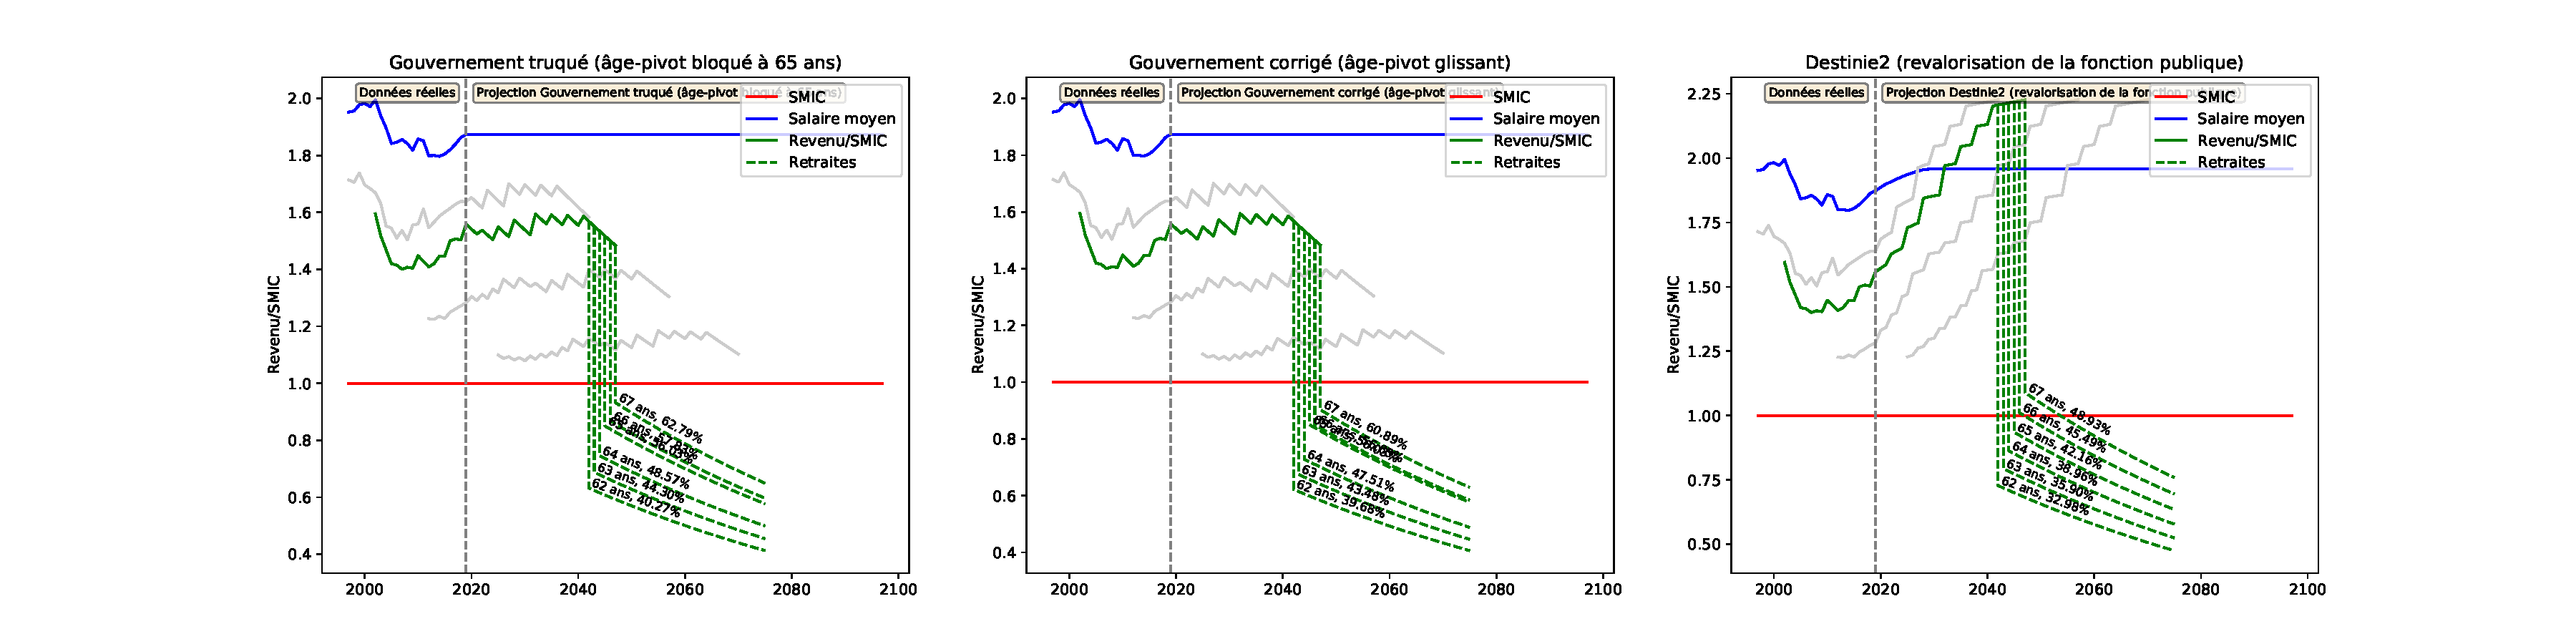
\includegraphics[width=0.9\textwidth]{fig/Redacteur_1980_22_dest_retraite.pdf}\end{center} \label{fig/Redacteur_1980_22_dest_retraite.pdf} 

\newpage 
 
\subsection{Génération 1990 (début en 2012)} 

\paragraph{Retraites possibles et ratios Revenu/SMIC à 70, 75, 80, 85, 90 ans avec le modèle \emph{Gouvernement truqué (âge-pivot bloqué à 65 ans)}}  
 
{ \scriptsize \begin{center} 
\begin{tabular}[htb]{|c|c||c|c||c|c||c||c|c|c|c|c|c|} 
\hline 
 Retraite en &  Âge &  Âge pivot &  Décote/Surcote &  Retraite (\euro{} 2019) &  Tx Rempl(\%) &  SMIC (\euro{} 2019) &  Retraite/SMIC &  Rev70/SMIC &  Rev75/SMIC &  Rev80/SMIC &  Rev85/SMIC &  Rev90/SMIC \\ 
\hline \hline 
 2052 &  62 &  65 ans 0 mois &  -15.00\% &  1546.31 &  {\bf 43.12} &  2601.14 &  {\bf {\color{red} 0.59}} &  {\bf {\color{red} 0.54}} &  {\bf {\color{red} 0.50}} &  {\bf {\color{red} 0.47}} &  {\bf {\color{red} 0.44}} &  {\bf {\color{red} 0.41}} \\ 
\hline 
 2053 &  63 &  65 ans 0 mois &  -10.00\% &  1703.55 &  {\bf 47.42} &  2634.96 &  {\bf {\color{red} 0.65}} &  {\bf {\color{red} 0.59}} &  {\bf {\color{red} 0.55}} &  {\bf {\color{red} 0.52}} &  {\bf {\color{red} 0.49}} &  {\bf {\color{red} 0.46}} \\ 
\hline 
 2054 &  64 &  65 ans 0 mois &  -5.00\% &  1869.16 &  {\bf 51.94} &  2669.21 &  {\bf {\color{red} 0.70}} &  {\bf {\color{red} 0.65}} &  {\bf {\color{red} 0.61}} &  {\bf {\color{red} 0.57}} &  {\bf {\color{red} 0.53}} &  {\bf {\color{red} 0.50}} \\ 
\hline 
 2055 &  65 &  65 ans 0 mois &  0.00\% &  2298.33 &  {\bf 63.75} &  2703.91 &  {\bf {\color{red} 0.85}} &  {\bf {\color{red} 0.80}} &  {\bf {\color{red} 0.75}} &  {\bf {\color{red} 0.70}} &  {\bf {\color{red} 0.66}} &  {\bf {\color{red} 0.62}} \\ 
\hline 
 2056 &  66 &  65 ans 0 mois &  5.00\% &  2328.20 &  {\bf 64.46} &  2739.06 &  {\bf {\color{red} 0.85}} &  {\bf {\color{red} 0.81}} &  {\bf {\color{red} 0.76}} &  {\bf {\color{red} 0.71}} &  {\bf {\color{red} 0.67}} &  {\bf {\color{red} 0.62}} \\ 
\hline 
 2057 &  67 &  65 ans 0 mois &  10.00\% &  2417.86 &  {\bf 66.83} &  2774.67 &  {\bf {\color{red} 0.87}} &  {\bf {\color{red} 0.84}} &  {\bf {\color{red} 0.79}} &  {\bf {\color{red} 0.74}} &  {\bf {\color{red} 0.69}} &  {\bf {\color{red} 0.65}} \\ 
\hline 
\hline 
\end{tabular} 
\end{center} } 
\paragraph{Retraites possibles et ratios Revenu/SMIC à 70, 75, 80, 85, 90 ans avec le modèle \emph{Gouvernement corrigé (âge-pivot glissant)}}  
 
{ \scriptsize \begin{center} 
\begin{tabular}[htb]{|c|c||c|c||c|c||c||c|c|c|c|c|c|} 
\hline 
 Retraite en &  Âge &  Âge pivot &  Décote/Surcote &  Retraite (\euro{} 2019) &  Tx Rempl(\%) &  SMIC (\euro{} 2019) &  Retraite/SMIC &  Rev70/SMIC &  Rev75/SMIC &  Rev80/SMIC &  Rev85/SMIC &  Rev90/SMIC \\ 
\hline \hline 
 2052 &  62 &  66 ans 1 mois &  -20.42\% &  1447.77 &  {\bf 40.38} &  2601.14 &  {\bf {\color{red} 0.56}} &  {\bf {\color{red} 0.50}} &  {\bf {\color{red} 0.47}} &  {\bf {\color{red} 0.44}} &  {\bf {\color{red} 0.41}} &  {\bf {\color{red} 0.39}} \\ 
\hline 
 2053 &  63 &  66 ans 2 mois &  -15.83\% &  1593.14 &  {\bf 44.35} &  2634.96 &  {\bf {\color{red} 0.60}} &  {\bf {\color{red} 0.55}} &  {\bf {\color{red} 0.52}} &  {\bf {\color{red} 0.49}} &  {\bf {\color{red} 0.46}} &  {\bf {\color{red} 0.43}} \\ 
\hline 
 2054 &  64 &  66 ans 3 mois &  -11.25\% &  1746.19 &  {\bf 48.52} &  2669.21 &  {\bf {\color{red} 0.65}} &  {\bf {\color{red} 0.61}} &  {\bf {\color{red} 0.57}} &  {\bf {\color{red} 0.53}} &  {\bf {\color{red} 0.50}} &  {\bf {\color{red} 0.47}} \\ 
\hline 
 2055 &  65 &  66 ans 4 mois &  -6.67\% &  2298.33 &  {\bf 63.75} &  2703.91 &  {\bf {\color{red} 0.85}} &  {\bf {\color{red} 0.80}} &  {\bf {\color{red} 0.75}} &  {\bf {\color{red} 0.70}} &  {\bf {\color{red} 0.66}} &  {\bf {\color{red} 0.62}} \\ 
\hline 
 2056 &  66 &  66 ans 5 mois &  -2.08\% &  2328.20 &  {\bf 64.46} &  2739.06 &  {\bf {\color{red} 0.85}} &  {\bf {\color{red} 0.81}} &  {\bf {\color{red} 0.76}} &  {\bf {\color{red} 0.71}} &  {\bf {\color{red} 0.67}} &  {\bf {\color{red} 0.62}} \\ 
\hline 
 2057 &  67 &  66 ans 6 mois &  2.50\% &  2358.47 &  {\bf 65.19} &  2774.67 &  {\bf {\color{red} 0.85}} &  {\bf {\color{red} 0.82}} &  {\bf {\color{red} 0.77}} &  {\bf {\color{red} 0.72}} &  {\bf {\color{red} 0.67}} &  {\bf {\color{red} 0.63}} \\ 
\hline 
\hline 
\end{tabular} 
\end{center} } 
\paragraph{Retraites possibles et ratios Revenu/SMIC à 70, 75, 80, 85, 90 ans avec le modèle \emph{Destinie2 (revalorisation de la fonction publique)}}  
 
{ \scriptsize \begin{center} 
\begin{tabular}[htb]{|c|c||c|c||c|c||c||c|c|c|c|c|c|} 
\hline 
 Retraite en &  Âge &  Âge pivot &  Décote/Surcote &  Retraite (\euro{} 2019) &  Tx Rempl(\%) &  SMIC (\euro{} 2019) &  Retraite/SMIC &  Rev70/SMIC &  Rev75/SMIC &  Rev80/SMIC &  Rev85/SMIC &  Rev90/SMIC \\ 
\hline \hline 
 2052 &  62 &  66 ans 1 mois &  -20.42\% &  1813.85 &  {\bf 33.43} &  2445.56 &  {\bf {\color{red} 0.74}} &  {\bf {\color{red} 0.67}} &  {\bf {\color{red} 0.63}} &  {\bf {\color{red} 0.59}} &  {\bf {\color{red} 0.55}} &  {\bf {\color{red} 0.52}} \\ 
\hline 
 2053 &  63 &  66 ans 2 mois &  -15.83\% &  2007.64 &  {\bf 36.53} &  2477.35 &  {\bf {\color{red} 0.81}} &  {\bf {\color{red} 0.74}} &  {\bf {\color{red} 0.69}} &  {\bf {\color{red} 0.65}} &  {\bf {\color{red} 0.61}} &  {\bf {\color{red} 0.57}} \\ 
\hline 
 2054 &  64 &  66 ans 3 mois &  -11.25\% &  2213.27 &  {\bf 39.75} &  2509.56 &  {\bf {\color{red} 0.88}} &  {\bf {\color{red} 0.82}} &  {\bf {\color{red} 0.77}} &  {\bf {\color{red} 0.72}} &  {\bf {\color{red} 0.67}} &  {\bf {\color{red} 0.63}} \\ 
\hline 
 2055 &  65 &  66 ans 4 mois &  -6.67\% &  2431.11 &  {\bf 43.10} &  2542.18 &  {\bf {\color{red} 0.96}} &  {\bf {\color{red} 0.90}} &  {\bf {\color{red} 0.84}} &  {\bf {\color{red} 0.79}} &  {\bf {\color{red} 0.74}} &  {\bf {\color{red} 0.69}} \\ 
\hline 
 2056 &  66 &  66 ans 5 mois &  -2.08\% &  2661.53 &  {\bf 46.58} &  2575.23 &  {\bf 1.03} &  {\bf {\color{red} 0.98}} &  {\bf {\color{red} 0.92}} &  {\bf {\color{red} 0.86}} &  {\bf {\color{red} 0.81}} &  {\bf {\color{red} 0.76}} \\ 
\hline 
 2057 &  67 &  66 ans 6 mois &  2.50\% &  2904.91 &  {\bf 50.19} &  2608.71 &  {\bf 1.11} &  {\bf 1.07} &  {\bf 1.00} &  {\bf {\color{red} 0.94}} &  {\bf {\color{red} 0.88}} &  {\bf {\color{red} 0.83}} \\ 
\hline 
\hline 
\end{tabular} 
\end{center} } 

 \begin{center}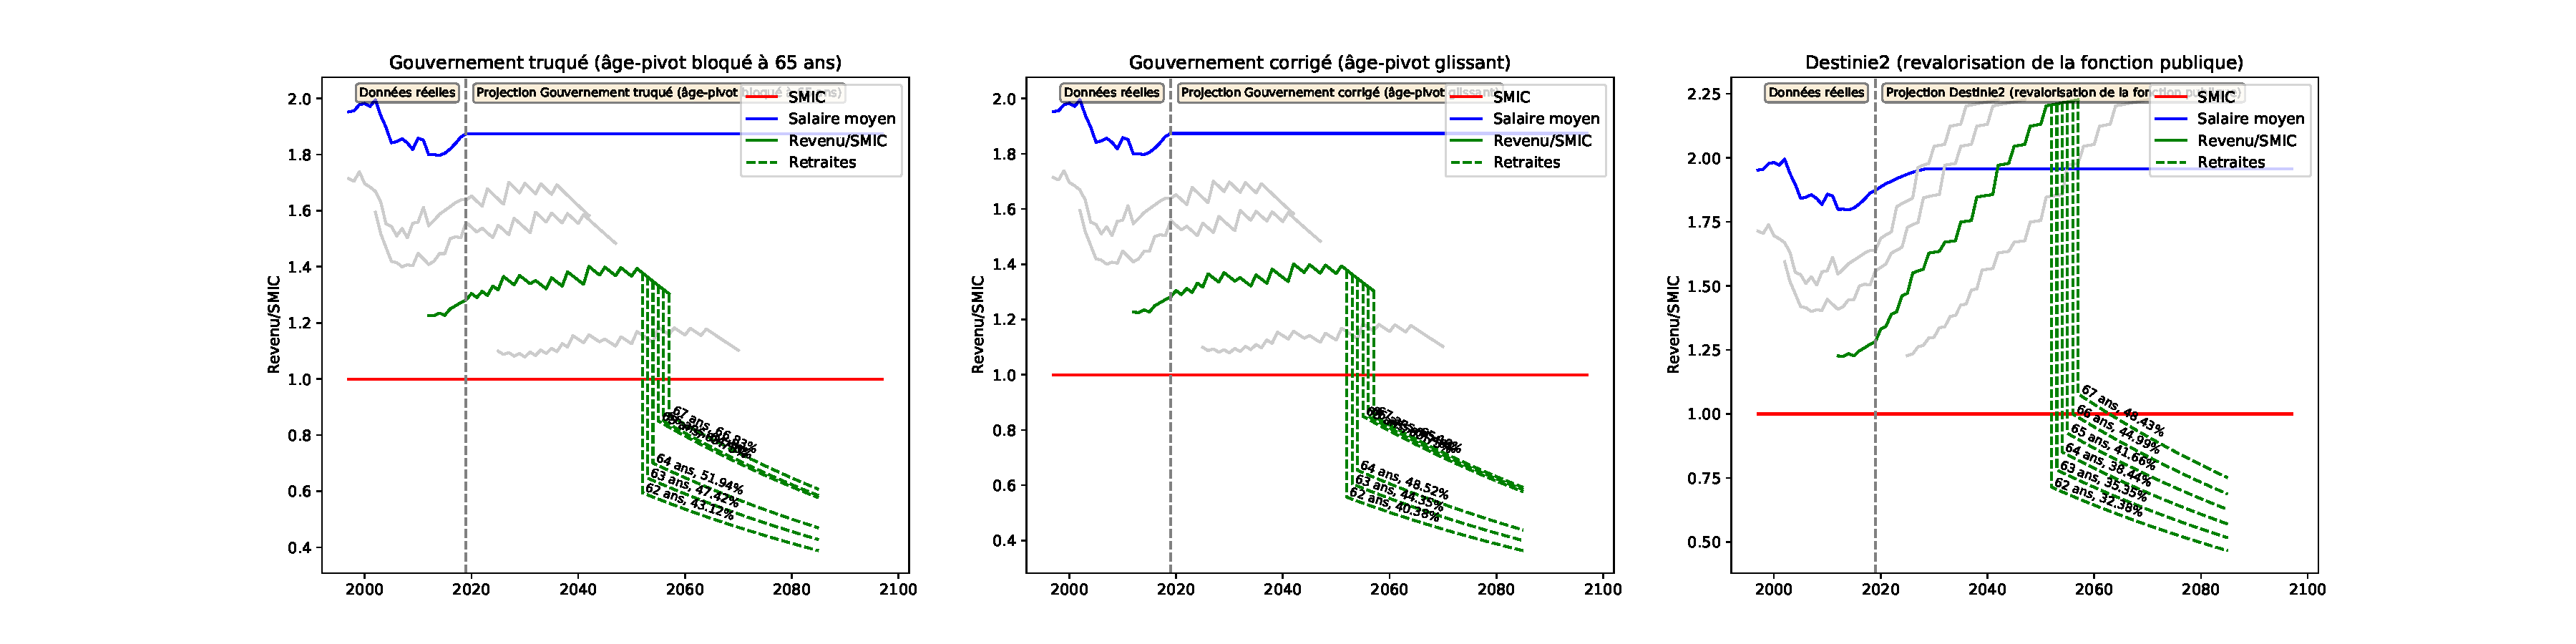
\includegraphics[width=0.9\textwidth]{fig/Redacteur_1990_22_dest_retraite.pdf}\end{center} \label{fig/Redacteur_1990_22_dest_retraite.pdf} 

\newpage 
 
\subsection{Génération 2003 (début en 2025)} 

\paragraph{Retraites possibles et ratios Revenu/SMIC à 70, 75, 80, 85, 90 ans avec le modèle \emph{Gouvernement truqué (âge-pivot bloqué à 65 ans)}}  
 
{ \scriptsize \begin{center} 
\begin{tabular}[htb]{|c|c||c|c||c|c||c||c|c|c|c|c|c|} 
\hline 
 Retraite en &  Âge &  Âge pivot &  Décote/Surcote &  Retraite (\euro{} 2019) &  Tx Rempl(\%) &  SMIC (\euro{} 2019) &  Retraite/SMIC &  Rev70/SMIC &  Rev75/SMIC &  Rev80/SMIC &  Rev85/SMIC &  Rev90/SMIC \\ 
\hline \hline 
 2065 &  62 &  65 ans 0 mois &  -15.00\% &  1653.71 &  {\bf 46.12} &  3076.71 &  {\bf {\color{red} 0.54}} &  {\bf {\color{red} 0.48}} &  {\bf {\color{red} 0.45}} &  {\bf {\color{red} 0.43}} &  {\bf {\color{red} 0.40}} &  {\bf {\color{red} 0.37}} \\ 
\hline 
 2066 &  63 &  65 ans 0 mois &  -10.00\% &  1818.75 &  {\bf 50.63} &  3116.71 &  {\bf {\color{red} 0.58}} &  {\bf {\color{red} 0.53}} &  {\bf {\color{red} 0.50}} &  {\bf {\color{red} 0.47}} &  {\bf {\color{red} 0.44}} &  {\bf {\color{red} 0.41}} \\ 
\hline 
 2067 &  64 &  65 ans 0 mois &  -5.00\% &  1992.34 &  {\bf 55.36} &  3157.23 &  {\bf {\color{red} 0.63}} &  {\bf {\color{red} 0.58}} &  {\bf {\color{red} 0.55}} &  {\bf {\color{red} 0.51}} &  {\bf {\color{red} 0.48}} &  {\bf {\color{red} 0.45}} \\ 
\hline 
 2068 &  65 &  65 ans 0 mois &  0.00\% &  2718.53 &  {\bf 75.41} &  3198.27 &  {\bf {\color{red} 0.85}} &  {\bf {\color{red} 0.80}} &  {\bf {\color{red} 0.75}} &  {\bf {\color{red} 0.70}} &  {\bf {\color{red} 0.66}} &  {\bf {\color{red} 0.62}} \\ 
\hline 
 2069 &  66 &  65 ans 0 mois &  5.00\% &  2753.87 &  {\bf 76.25} &  3239.85 &  {\bf {\color{red} 0.85}} &  {\bf {\color{red} 0.81}} &  {\bf {\color{red} 0.76}} &  {\bf {\color{red} 0.71}} &  {\bf {\color{red} 0.67}} &  {\bf {\color{red} 0.62}} \\ 
\hline 
 2070 &  67 &  65 ans 0 mois &  10.00\% &  2789.67 &  {\bf 77.10} &  3281.97 &  {\bf {\color{red} 0.85}} &  {\bf {\color{red} 0.82}} &  {\bf {\color{red} 0.77}} &  {\bf {\color{red} 0.72}} &  {\bf {\color{red} 0.67}} &  {\bf {\color{red} 0.63}} \\ 
\hline 
\hline 
\end{tabular} 
\end{center} } 
\paragraph{Retraites possibles et ratios Revenu/SMIC à 70, 75, 80, 85, 90 ans avec le modèle \emph{Gouvernement corrigé (âge-pivot glissant)}}  
 
{ \scriptsize \begin{center} 
\begin{tabular}[htb]{|c|c||c|c||c|c||c||c|c|c|c|c|c|} 
\hline 
 Retraite en &  Âge &  Âge pivot &  Décote/Surcote &  Retraite (\euro{} 2019) &  Tx Rempl(\%) &  SMIC (\euro{} 2019) &  Retraite/SMIC &  Rev70/SMIC &  Rev75/SMIC &  Rev80/SMIC &  Rev85/SMIC &  Rev90/SMIC \\ 
\hline \hline 
 2065 &  62 &  67 ans 2 mois &  -25.83\% &  1442.94 &  {\bf 40.24} &  3076.71 &  {\bf {\color{red} 0.47}} &  {\bf {\color{red} 0.42}} &  {\bf {\color{red} 0.40}} &  {\bf {\color{red} 0.37}} &  {\bf {\color{red} 0.35}} &  {\bf {\color{red} 0.33}} \\ 
\hline 
 2066 &  63 &  67 ans 3 mois &  -21.25\% &  1591.41 &  {\bf 44.30} &  3116.71 &  {\bf {\color{red} 0.51}} &  {\bf {\color{red} 0.47}} &  {\bf {\color{red} 0.44}} &  {\bf {\color{red} 0.41}} &  {\bf {\color{red} 0.38}} &  {\bf {\color{red} 0.36}} \\ 
\hline 
 2067 &  64 &  67 ans 4 mois &  -16.67\% &  1747.66 &  {\bf 48.56} &  3157.23 &  {\bf {\color{red} 0.55}} &  {\bf {\color{red} 0.51}} &  {\bf {\color{red} 0.48}} &  {\bf {\color{red} 0.45}} &  {\bf {\color{red} 0.42}} &  {\bf {\color{red} 0.40}} \\ 
\hline 
 2068 &  65 &  67 ans 5 mois &  -12.08\% &  2718.53 &  {\bf 75.41} &  3198.27 &  {\bf {\color{red} 0.85}} &  {\bf {\color{red} 0.80}} &  {\bf {\color{red} 0.75}} &  {\bf {\color{red} 0.70}} &  {\bf {\color{red} 0.66}} &  {\bf {\color{red} 0.62}} \\ 
\hline 
 2069 &  66 &  67 ans 6 mois &  -7.50\% &  2753.87 &  {\bf 76.25} &  3239.85 &  {\bf {\color{red} 0.85}} &  {\bf {\color{red} 0.81}} &  {\bf {\color{red} 0.76}} &  {\bf {\color{red} 0.71}} &  {\bf {\color{red} 0.67}} &  {\bf {\color{red} 0.62}} \\ 
\hline 
 2070 &  67 &  67 ans 7 mois &  -2.92\% &  2789.67 &  {\bf 77.10} &  3281.97 &  {\bf {\color{red} 0.85}} &  {\bf {\color{red} 0.82}} &  {\bf {\color{red} 0.77}} &  {\bf {\color{red} 0.72}} &  {\bf {\color{red} 0.67}} &  {\bf {\color{red} 0.63}} \\ 
\hline 
\hline 
\end{tabular} 
\end{center} } 
\paragraph{Retraites possibles et ratios Revenu/SMIC à 70, 75, 80, 85, 90 ans avec le modèle \emph{Destinie2 (revalorisation de la fonction publique)}}  
 
{ \scriptsize \begin{center} 
\begin{tabular}[htb]{|c|c||c|c||c|c||c||c|c|c|c|c|c|} 
\hline 
 Retraite en &  Âge &  Âge pivot &  Décote/Surcote &  Retraite (\euro{} 2019) &  Tx Rempl(\%) &  SMIC (\euro{} 2019) &  Retraite/SMIC &  Rev70/SMIC &  Rev75/SMIC &  Rev80/SMIC &  Rev85/SMIC &  Rev90/SMIC \\ 
\hline \hline 
 2065 &  62 &  67 ans 2 mois &  -25.83\% &  2102.63 &  {\bf 32.76} &  2892.68 &  {\bf {\color{red} 0.73}} &  {\bf {\color{red} 0.66}} &  {\bf {\color{red} 0.61}} &  {\bf {\color{red} 0.58}} &  {\bf {\color{red} 0.54}} &  {\bf {\color{red} 0.51}} \\ 
\hline 
 2066 &  63 &  67 ans 3 mois &  -21.25\% &  2332.85 &  {\bf 35.88} &  2930.29 &  {\bf {\color{red} 0.80}} &  {\bf {\color{red} 0.73}} &  {\bf {\color{red} 0.68}} &  {\bf {\color{red} 0.64}} &  {\bf {\color{red} 0.60}} &  {\bf {\color{red} 0.56}} \\ 
\hline 
 2067 &  64 &  67 ans 4 mois &  -16.67\% &  2577.11 &  {\bf 39.13} &  2968.38 &  {\bf {\color{red} 0.87}} &  {\bf {\color{red} 0.80}} &  {\bf {\color{red} 0.75}} &  {\bf {\color{red} 0.71}} &  {\bf {\color{red} 0.66}} &  {\bf {\color{red} 0.62}} \\ 
\hline 
 2068 &  65 &  67 ans 5 mois &  -12.08\% &  2835.84 &  {\bf 42.51} &  3006.97 &  {\bf {\color{red} 0.94}} &  {\bf {\color{red} 0.88}} &  {\bf {\color{red} 0.83}} &  {\bf {\color{red} 0.78}} &  {\bf {\color{red} 0.73}} &  {\bf {\color{red} 0.68}} \\ 
\hline 
 2069 &  66 &  67 ans 6 mois &  -7.50\% &  3109.49 &  {\bf 46.01} &  3046.06 &  {\bf 1.02} &  {\bf {\color{red} 0.97}} &  {\bf {\color{red} 0.91}} &  {\bf {\color{red} 0.85}} &  {\bf {\color{red} 0.80}} &  {\bf {\color{red} 0.75}} \\ 
\hline 
 2070 &  67 &  67 ans 7 mois &  -2.92\% &  3398.50 &  {\bf 49.64} &  3085.66 &  {\bf 1.10} &  {\bf 1.06} &  {\bf {\color{red} 0.99}} &  {\bf {\color{red} 0.93}} &  {\bf {\color{red} 0.87}} &  {\bf {\color{red} 0.82}} \\ 
\hline 
\hline 
\end{tabular} 
\end{center} } 

 \begin{center}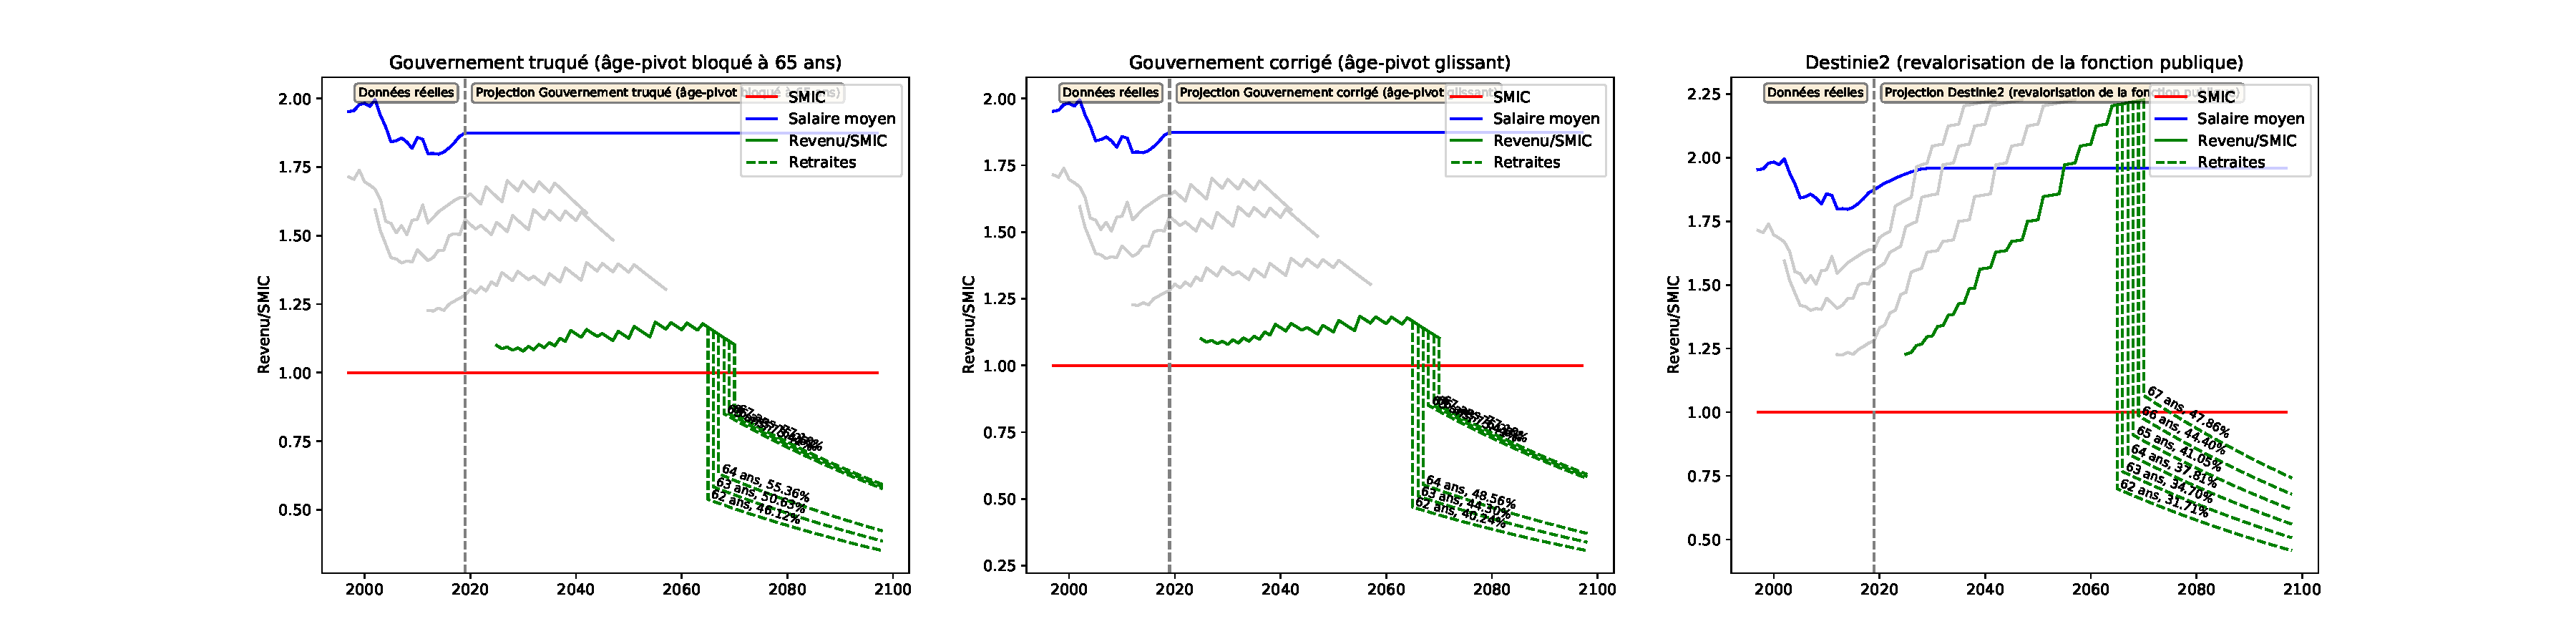
\includegraphics[width=0.9\textwidth]{fig/Redacteur_2003_22_dest_retraite.pdf}\end{center} \label{fig/Redacteur_2003_22_dest_retraite.pdf} 

\newpage 
 
\chapter{Secrétaire administratif} 

\begin{minipage}{0.55\linewidth}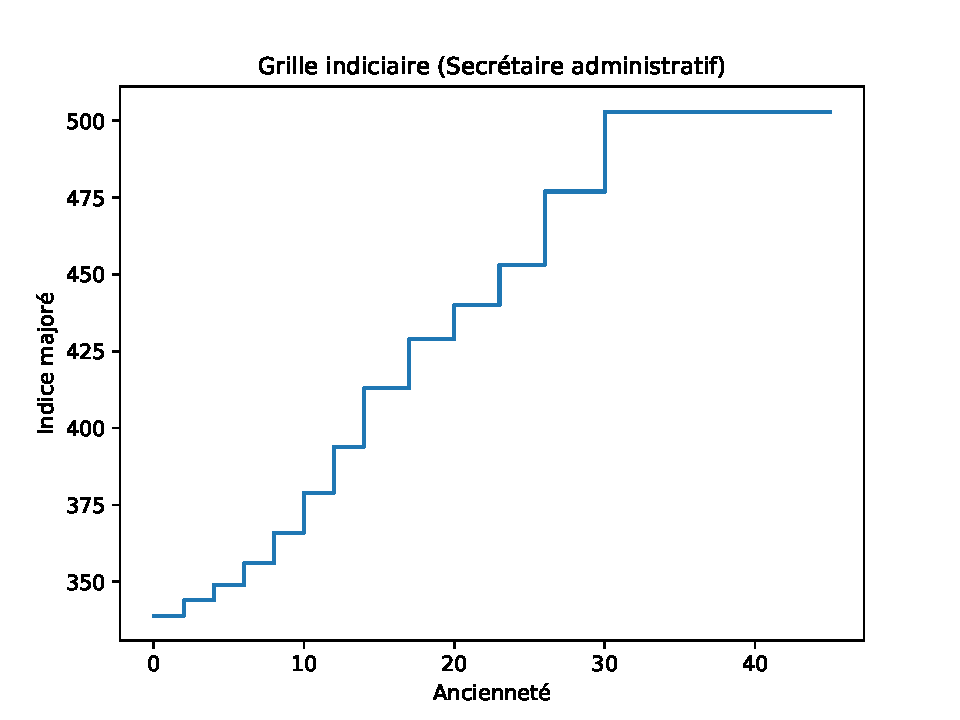
\includegraphics[width=0.7\textwidth]{fig/grille_SecretaireAdmin.pdf}\end{minipage} 
\begin{minipage}{0.3\linewidth} 
 \begin{center} 

\begin{tabular}[htb]{|c|c|} 
\hline 
 Indice majoré &  Durée (années) \\ 
\hline \hline 
 339 &  2.00 \\ 
\hline 
 344 &  2.00 \\ 
\hline 
 349 &  2.00 \\ 
\hline 
 356 &  2.00 \\ 
\hline 
 366 &  2.00 \\ 
\hline 
 379 &  2.00 \\ 
\hline 
 394 &  2.00 \\ 
\hline 
 413 &  3.00 \\ 
\hline 
 429 &  3.00 \\ 
\hline 
 440 &  3.00 \\ 
\hline 
 453 &  3.00 \\ 
\hline 
 477 &  4.00 \\ 
\hline 
 503 &   \\ 
\hline 
\hline 
\end{tabular} 
\end{center} 
 \end{minipage} 


 \addto{\captionsenglish}{ \renewcommand{\mtctitle}{}} \setcounter{minitocdepth}{2} 
 \minitoc \newpage 

\section{Début de carrière à 22 ans} 

\subsection{Génération 1975 (début en 1997)} 

\paragraph{Retraites possibles et ratios Revenu/SMIC à 70, 75, 80, 85, 90 ans avec le modèle \emph{Gouvernement truqué (âge-pivot bloqué à 65 ans)}}  
 
{ \scriptsize \begin{center} 
\begin{tabular}[htb]{|c|c||c|c||c|c||c||c|c|c|c|c|c|} 
\hline 
 Retraite en &  Âge &  Âge pivot &  Décote/Surcote &  Retraite (\euro{} 2019) &  Tx Rempl(\%) &  SMIC (\euro{} 2019) &  Retraite/SMIC &  Rev70/SMIC &  Rev75/SMIC &  Rev80/SMIC &  Rev85/SMIC &  Rev90/SMIC \\ 
\hline \hline 
 2037 &  62 &  64 ans 10 mois &  -14.17\% &  1465.93 &  {\bf 43.54} &  2143.00 &  {\bf {\color{red} 0.68}} &  {\bf {\color{red} 0.62}} &  {\bf {\color{red} 0.58}} &  {\bf {\color{red} 0.54}} &  {\bf {\color{red} 0.51}} &  {\bf {\color{red} 0.48}} \\ 
\hline 
 2038 &  63 &  64 ans 11 mois &  -9.58\% &  1598.43 &  {\bf 47.40} &  2170.86 &  {\bf {\color{red} 0.74}} &  {\bf {\color{red} 0.67}} &  {\bf {\color{red} 0.63}} &  {\bf {\color{red} 0.59}} &  {\bf {\color{red} 0.55}} &  {\bf {\color{red} 0.52}} \\ 
\hline 
 2039 &  64 &  65 ans 0 mois &  -5.00\% &  1738.22 &  {\bf 51.46} &  2199.08 &  {\bf {\color{red} 0.79}} &  {\bf {\color{red} 0.73}} &  {\bf {\color{red} 0.69}} &  {\bf {\color{red} 0.64}} &  {\bf {\color{red} 0.60}} &  {\bf {\color{red} 0.56}} \\ 
\hline 
 2040 &  65 &  65 ans 0 mois &  0.00\% &  1893.56 &  {\bf 55.97} &  2227.67 &  {\bf {\color{red} 0.85}} &  {\bf {\color{red} 0.80}} &  {\bf {\color{red} 0.75}} &  {\bf {\color{red} 0.70}} &  {\bf {\color{red} 0.66}} &  {\bf {\color{red} 0.62}} \\ 
\hline 
 2041 &  66 &  65 ans 0 mois &  5.00\% &  2057.51 &  {\bf 60.71} &  2256.63 &  {\bf {\color{red} 0.91}} &  {\bf {\color{red} 0.87}} &  {\bf {\color{red} 0.81}} &  {\bf {\color{red} 0.76}} &  {\bf {\color{red} 0.71}} &  {\bf {\color{red} 0.67}} \\ 
\hline 
 2042 &  67 &  65 ans 0 mois &  10.00\% &  2230.51 &  {\bf 65.71} &  2285.97 &  {\bf {\color{red} 0.98}} &  {\bf {\color{red} 0.94}} &  {\bf {\color{red} 0.88}} &  {\bf {\color{red} 0.82}} &  {\bf {\color{red} 0.77}} &  {\bf {\color{red} 0.72}} \\ 
\hline 
\hline 
\end{tabular} 
\end{center} } 
\paragraph{Retraites possibles et ratios Revenu/SMIC à 70, 75, 80, 85, 90 ans avec le modèle \emph{Gouvernement corrigé (âge-pivot glissant)}}  
 
{ \scriptsize \begin{center} 
\begin{tabular}[htb]{|c|c||c|c||c|c||c||c|c|c|c|c|c|} 
\hline 
 Retraite en &  Âge &  Âge pivot &  Décote/Surcote &  Retraite (\euro{} 2019) &  Tx Rempl(\%) &  SMIC (\euro{} 2019) &  Retraite/SMIC &  Rev70/SMIC &  Rev75/SMIC &  Rev80/SMIC &  Rev85/SMIC &  Rev90/SMIC \\ 
\hline \hline 
 2037 &  62 &  64 ans 10 mois &  -14.17\% &  1465.93 &  {\bf 43.54} &  2143.00 &  {\bf {\color{red} 0.68}} &  {\bf {\color{red} 0.62}} &  {\bf {\color{red} 0.58}} &  {\bf {\color{red} 0.54}} &  {\bf {\color{red} 0.51}} &  {\bf {\color{red} 0.48}} \\ 
\hline 
 2038 &  63 &  64 ans 11 mois &  -9.58\% &  1598.43 &  {\bf 47.40} &  2170.86 &  {\bf {\color{red} 0.74}} &  {\bf {\color{red} 0.67}} &  {\bf {\color{red} 0.63}} &  {\bf {\color{red} 0.59}} &  {\bf {\color{red} 0.55}} &  {\bf {\color{red} 0.52}} \\ 
\hline 
 2039 &  64 &  65 ans 0 mois &  -5.00\% &  1738.22 &  {\bf 51.46} &  2199.08 &  {\bf {\color{red} 0.79}} &  {\bf {\color{red} 0.73}} &  {\bf {\color{red} 0.69}} &  {\bf {\color{red} 0.64}} &  {\bf {\color{red} 0.60}} &  {\bf {\color{red} 0.56}} \\ 
\hline 
 2040 &  65 &  65 ans 1 mois &  -0.42\% &  1893.52 &  {\bf 55.96} &  2227.67 &  {\bf {\color{red} 0.85}} &  {\bf {\color{red} 0.80}} &  {\bf {\color{red} 0.75}} &  {\bf {\color{red} 0.70}} &  {\bf {\color{red} 0.66}} &  {\bf {\color{red} 0.62}} \\ 
\hline 
 2041 &  66 &  65 ans 2 mois &  4.17\% &  2041.18 &  {\bf 60.23} &  2256.63 &  {\bf {\color{red} 0.90}} &  {\bf {\color{red} 0.86}} &  {\bf {\color{red} 0.81}} &  {\bf {\color{red} 0.75}} &  {\bf {\color{red} 0.71}} &  {\bf {\color{red} 0.66}} \\ 
\hline 
 2042 &  67 &  65 ans 3 mois &  8.75\% &  2205.16 &  {\bf 64.96} &  2285.97 &  {\bf {\color{red} 0.96}} &  {\bf {\color{red} 0.93}} &  {\bf {\color{red} 0.87}} &  {\bf {\color{red} 0.82}} &  {\bf {\color{red} 0.76}} &  {\bf {\color{red} 0.72}} \\ 
\hline 
\hline 
\end{tabular} 
\end{center} } 
\paragraph{Retraites possibles et ratios Revenu/SMIC à 70, 75, 80, 85, 90 ans avec le modèle \emph{Destinie2 (revalorisation de la fonction publique)}}  
 
{ \scriptsize \begin{center} 
\begin{tabular}[htb]{|c|c||c|c||c|c||c||c|c|c|c|c|c|} 
\hline 
 Retraite en &  Âge &  Âge pivot &  Décote/Surcote &  Retraite (\euro{} 2019) &  Tx Rempl(\%) &  SMIC (\euro{} 2019) &  Retraite/SMIC &  Rev70/SMIC &  Rev75/SMIC &  Rev80/SMIC &  Rev85/SMIC &  Rev90/SMIC \\ 
\hline \hline 
 2037 &  62 &  64 ans 10 mois &  -14.17\% &  1608.00 &  {\bf 38.33} &  2014.82 &  {\bf {\color{red} 0.80}} &  {\bf {\color{red} 0.72}} &  {\bf {\color{red} 0.67}} &  {\bf {\color{red} 0.63}} &  {\bf {\color{red} 0.59}} &  {\bf {\color{red} 0.56}} \\ 
\hline 
 2038 &  63 &  64 ans 11 mois &  -9.58\% &  1760.27 &  {\bf 41.42} &  2041.01 &  {\bf {\color{red} 0.86}} &  {\bf {\color{red} 0.79}} &  {\bf {\color{red} 0.74}} &  {\bf {\color{red} 0.69}} &  {\bf {\color{red} 0.65}} &  {\bf {\color{red} 0.61}} \\ 
\hline 
 2039 &  64 &  65 ans 0 mois &  -5.00\% &  1921.95 &  {\bf 44.64} &  2067.55 &  {\bf {\color{red} 0.93}} &  {\bf {\color{red} 0.86}} &  {\bf {\color{red} 0.81}} &  {\bf {\color{red} 0.76}} &  {\bf {\color{red} 0.71}} &  {\bf {\color{red} 0.66}} \\ 
\hline 
 2040 &  65 &  65 ans 1 mois &  -0.42\% &  2093.58 &  {\bf 48.01} &  2094.43 &  {\bf {\color{red} 1.00}} &  {\bf {\color{red} 0.94}} &  {\bf {\color{red} 0.88}} &  {\bf {\color{red} 0.82}} &  {\bf {\color{red} 0.77}} &  {\bf {\color{red} 0.72}} \\ 
\hline 
 2041 &  66 &  65 ans 2 mois &  4.17\% &  2275.73 &  {\bf 51.51} &  2121.65 &  {\bf 1.07} &  {\bf 1.02} &  {\bf {\color{red} 0.95}} &  {\bf {\color{red} 0.90}} &  {\bf {\color{red} 0.84}} &  {\bf {\color{red} 0.79}} \\ 
\hline 
 2042 &  67 &  65 ans 3 mois &  8.75\% &  2469.02 &  {\bf 55.17} &  2149.23 &  {\bf 1.15} &  {\bf 1.11} &  {\bf 1.04} &  {\bf {\color{red} 0.97}} &  {\bf {\color{red} 0.91}} &  {\bf {\color{red} 0.85}} \\ 
\hline 
\hline 
\end{tabular} 
\end{center} } 

 \begin{center}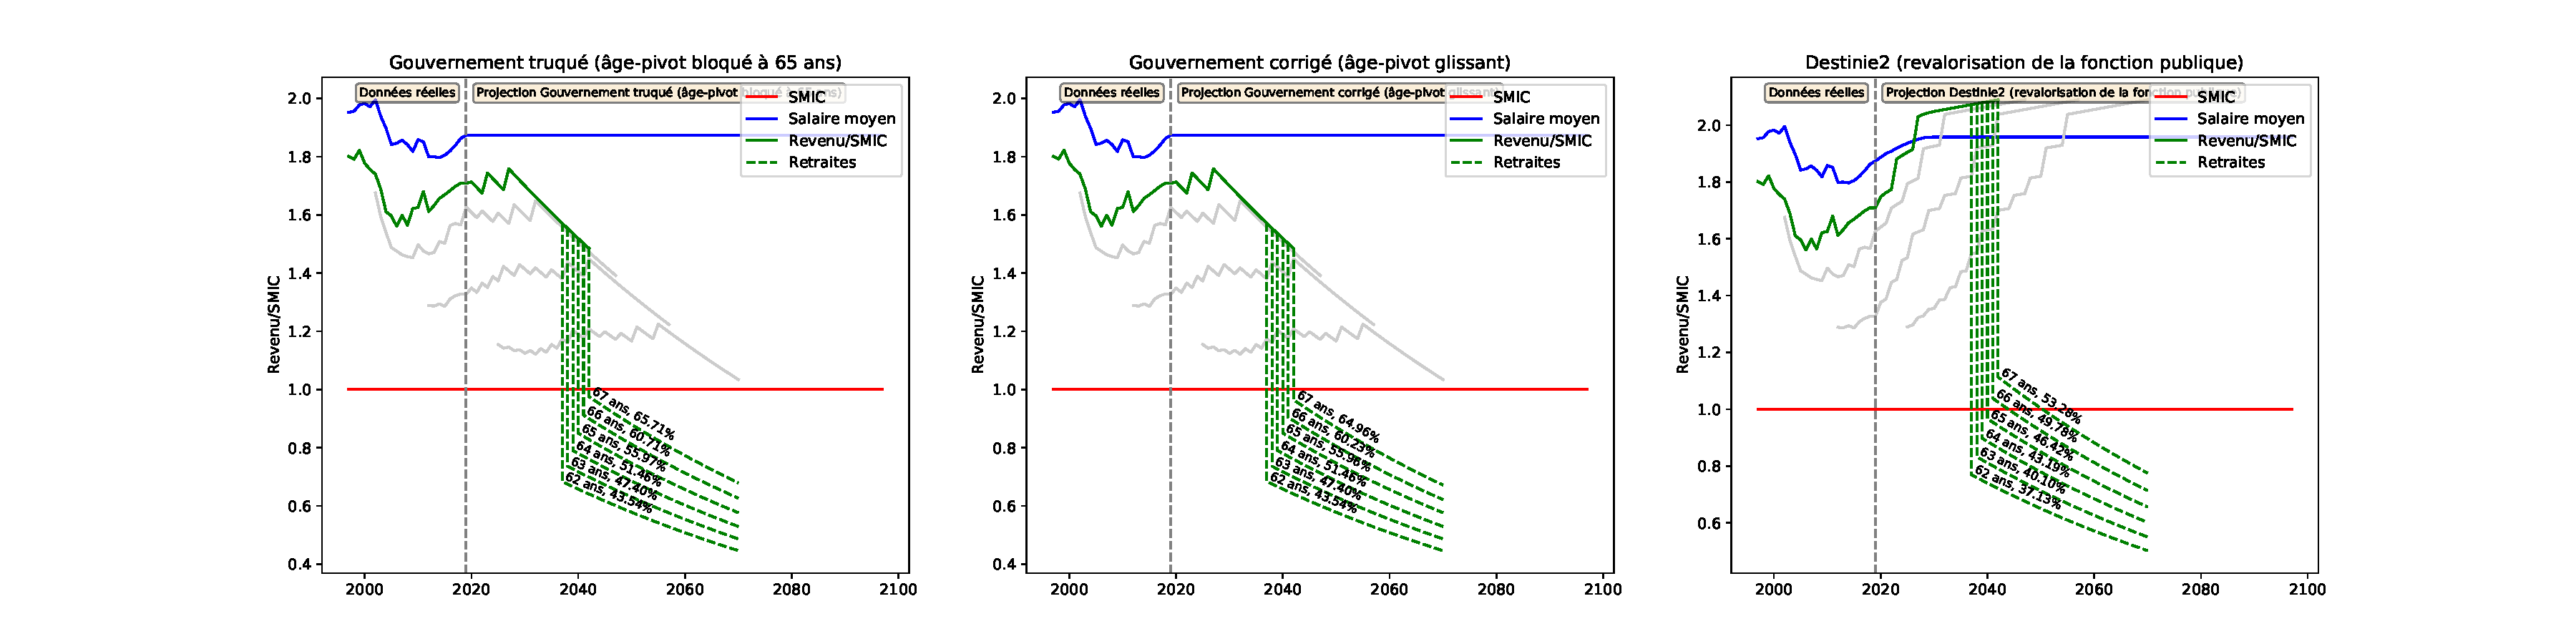
\includegraphics[width=0.9\textwidth]{fig/SecretaireAdmin_1975_22_dest_retraite.pdf}\end{center} \label{fig/SecretaireAdmin_1975_22_dest_retraite.pdf} 

\newpage 
 
\subsection{Génération 1980 (début en 2002)} 

\paragraph{Retraites possibles et ratios Revenu/SMIC à 70, 75, 80, 85, 90 ans avec le modèle \emph{Gouvernement truqué (âge-pivot bloqué à 65 ans)}}  
 
{ \scriptsize \begin{center} 
\begin{tabular}[htb]{|c|c||c|c||c|c||c||c|c|c|c|c|c|} 
\hline 
 Retraite en &  Âge &  Âge pivot &  Décote/Surcote &  Retraite (\euro{} 2019) &  Tx Rempl(\%) &  SMIC (\euro{} 2019) &  Retraite/SMIC &  Rev70/SMIC &  Rev75/SMIC &  Rev80/SMIC &  Rev85/SMIC &  Rev90/SMIC \\ 
\hline \hline 
 2042 &  62 &  65 ans 0 mois &  -15.00\% &  1480.11 &  {\bf 43.96} &  2285.97 &  {\bf {\color{red} 0.65}} &  {\bf {\color{red} 0.58}} &  {\bf {\color{red} 0.55}} &  {\bf {\color{red} 0.51}} &  {\bf {\color{red} 0.48}} &  {\bf {\color{red} 0.45}} \\ 
\hline 
 2043 &  63 &  65 ans 0 mois &  -10.00\% &  1627.38 &  {\bf 48.26} &  2315.68 &  {\bf {\color{red} 0.70}} &  {\bf {\color{red} 0.64}} &  {\bf {\color{red} 0.60}} &  {\bf {\color{red} 0.56}} &  {\bf {\color{red} 0.53}} &  {\bf {\color{red} 0.50}} \\ 
\hline 
 2044 &  64 &  65 ans 0 mois &  -5.00\% &  1783.47 &  {\bf 52.80} &  2345.79 &  {\bf {\color{red} 0.76}} &  {\bf {\color{red} 0.70}} &  {\bf {\color{red} 0.66}} &  {\bf {\color{red} 0.62}} &  {\bf {\color{red} 0.58}} &  {\bf {\color{red} 0.54}} \\ 
\hline 
 2045 &  65 &  65 ans 0 mois &  0.00\% &  2019.84 &  {\bf 59.70} &  2376.28 &  {\bf {\color{red} 0.85}} &  {\bf {\color{red} 0.80}} &  {\bf {\color{red} 0.75}} &  {\bf {\color{red} 0.70}} &  {\bf {\color{red} 0.66}} &  {\bf {\color{red} 0.62}} \\ 
\hline 
 2046 &  66 &  65 ans 0 mois &  5.00\% &  2122.41 &  {\bf 62.63} &  2407.18 &  {\bf {\color{red} 0.88}} &  {\bf {\color{red} 0.84}} &  {\bf {\color{red} 0.78}} &  {\bf {\color{red} 0.74}} &  {\bf {\color{red} 0.69}} &  {\bf {\color{red} 0.65}} \\ 
\hline 
 2047 &  67 &  65 ans 0 mois &  10.00\% &  2304.36 &  {\bf 67.88} &  2438.47 &  {\bf {\color{red} 0.95}} &  {\bf {\color{red} 0.91}} &  {\bf {\color{red} 0.85}} &  {\bf {\color{red} 0.80}} &  {\bf {\color{red} 0.75}} &  {\bf {\color{red} 0.70}} \\ 
\hline 
\hline 
\end{tabular} 
\end{center} } 
\paragraph{Retraites possibles et ratios Revenu/SMIC à 70, 75, 80, 85, 90 ans avec le modèle \emph{Gouvernement corrigé (âge-pivot glissant)}}  
 
{ \scriptsize \begin{center} 
\begin{tabular}[htb]{|c|c||c|c||c|c||c||c|c|c|c|c|c|} 
\hline 
 Retraite en &  Âge &  Âge pivot &  Décote/Surcote &  Retraite (\euro{} 2019) &  Tx Rempl(\%) &  SMIC (\euro{} 2019) &  Retraite/SMIC &  Rev70/SMIC &  Rev75/SMIC &  Rev80/SMIC &  Rev85/SMIC &  Rev90/SMIC \\ 
\hline \hline 
 2042 &  62 &  65 ans 3 mois &  -16.25\% &  1458.34 &  {\bf 43.31} &  2285.97 &  {\bf {\color{red} 0.64}} &  {\bf {\color{red} 0.58}} &  {\bf {\color{red} 0.54}} &  {\bf {\color{red} 0.51}} &  {\bf {\color{red} 0.47}} &  {\bf {\color{red} 0.44}} \\ 
\hline 
 2043 &  63 &  65 ans 4 mois &  -11.67\% &  1597.24 &  {\bf 47.36} &  2315.68 &  {\bf {\color{red} 0.69}} &  {\bf {\color{red} 0.63}} &  {\bf {\color{red} 0.59}} &  {\bf {\color{red} 0.55}} &  {\bf {\color{red} 0.52}} &  {\bf {\color{red} 0.49}} \\ 
\hline 
 2044 &  64 &  65 ans 5 mois &  -7.08\% &  1744.36 &  {\bf 51.64} &  2345.79 &  {\bf {\color{red} 0.74}} &  {\bf {\color{red} 0.69}} &  {\bf {\color{red} 0.65}} &  {\bf {\color{red} 0.60}} &  {\bf {\color{red} 0.57}} &  {\bf {\color{red} 0.53}} \\ 
\hline 
 2045 &  65 &  65 ans 6 mois &  -2.50\% &  2019.84 &  {\bf 59.70} &  2376.28 &  {\bf {\color{red} 0.85}} &  {\bf {\color{red} 0.80}} &  {\bf {\color{red} 0.75}} &  {\bf {\color{red} 0.70}} &  {\bf {\color{red} 0.66}} &  {\bf {\color{red} 0.62}} \\ 
\hline 
 2046 &  66 &  65 ans 7 mois &  2.08\% &  2063.45 &  {\bf 60.89} &  2407.18 &  {\bf {\color{red} 0.86}} &  {\bf {\color{red} 0.81}} &  {\bf {\color{red} 0.76}} &  {\bf {\color{red} 0.72}} &  {\bf {\color{red} 0.67}} &  {\bf {\color{red} 0.63}} \\ 
\hline 
 2047 &  67 &  65 ans 8 mois &  6.67\% &  2234.53 &  {\bf 65.83} &  2438.47 &  {\bf {\color{red} 0.92}} &  {\bf {\color{red} 0.88}} &  {\bf {\color{red} 0.83}} &  {\bf {\color{red} 0.77}} &  {\bf {\color{red} 0.73}} &  {\bf {\color{red} 0.68}} \\ 
\hline 
\hline 
\end{tabular} 
\end{center} } 
\paragraph{Retraites possibles et ratios Revenu/SMIC à 70, 75, 80, 85, 90 ans avec le modèle \emph{Destinie2 (revalorisation de la fonction publique)}}  
 
{ \scriptsize \begin{center} 
\begin{tabular}[htb]{|c|c||c|c||c|c||c||c|c|c|c|c|c|} 
\hline 
 Retraite en &  Âge &  Âge pivot &  Décote/Surcote &  Retraite (\euro{} 2019) &  Tx Rempl(\%) &  SMIC (\euro{} 2019) &  Retraite/SMIC &  Rev70/SMIC &  Rev75/SMIC &  Rev80/SMIC &  Rev85/SMIC &  Rev90/SMIC \\ 
\hline \hline 
 2042 &  62 &  65 ans 3 mois &  -16.25\% &  1656.45 &  {\bf 37.01} &  2149.23 &  {\bf {\color{red} 0.77}} &  {\bf {\color{red} 0.70}} &  {\bf {\color{red} 0.65}} &  {\bf {\color{red} 0.61}} &  {\bf {\color{red} 0.57}} &  {\bf {\color{red} 0.54}} \\ 
\hline 
 2043 &  63 &  65 ans 4 mois &  -11.67\% &  1822.87 &  {\bf 40.21} &  2177.17 &  {\bf {\color{red} 0.84}} &  {\bf {\color{red} 0.76}} &  {\bf {\color{red} 0.72}} &  {\bf {\color{red} 0.67}} &  {\bf {\color{red} 0.63}} &  {\bf {\color{red} 0.59}} \\ 
\hline 
 2044 &  64 &  65 ans 5 mois &  -7.08\% &  2000.30 &  {\bf 43.56} &  2205.48 &  {\bf {\color{red} 0.91}} &  {\bf {\color{red} 0.84}} &  {\bf {\color{red} 0.79}} &  {\bf {\color{red} 0.74}} &  {\bf {\color{red} 0.69}} &  {\bf {\color{red} 0.65}} \\ 
\hline 
 2045 &  65 &  65 ans 6 mois &  -2.50\% &  2189.39 &  {\bf 47.06} &  2234.15 &  {\bf {\color{red} 0.98}} &  {\bf {\color{red} 0.92}} &  {\bf {\color{red} 0.86}} &  {\bf {\color{red} 0.81}} &  {\bf {\color{red} 0.76}} &  {\bf {\color{red} 0.71}} \\ 
\hline 
 2046 &  66 &  65 ans 7 mois &  2.08\% &  2389.08 &  {\bf 50.70} &  2263.19 &  {\bf 1.06} &  {\bf 1.00} &  {\bf {\color{red} 0.94}} &  {\bf {\color{red} 0.88}} &  {\bf {\color{red} 0.83}} &  {\bf {\color{red} 0.77}} \\ 
\hline 
 2047 &  67 &  65 ans 8 mois &  6.67\% &  2599.67 &  {\bf 54.46} &  2292.61 &  {\bf 1.13} &  {\bf 1.09} &  {\bf 1.02} &  {\bf {\color{red} 0.96}} &  {\bf {\color{red} 0.90}} &  {\bf {\color{red} 0.84}} \\ 
\hline 
\hline 
\end{tabular} 
\end{center} } 

 \begin{center}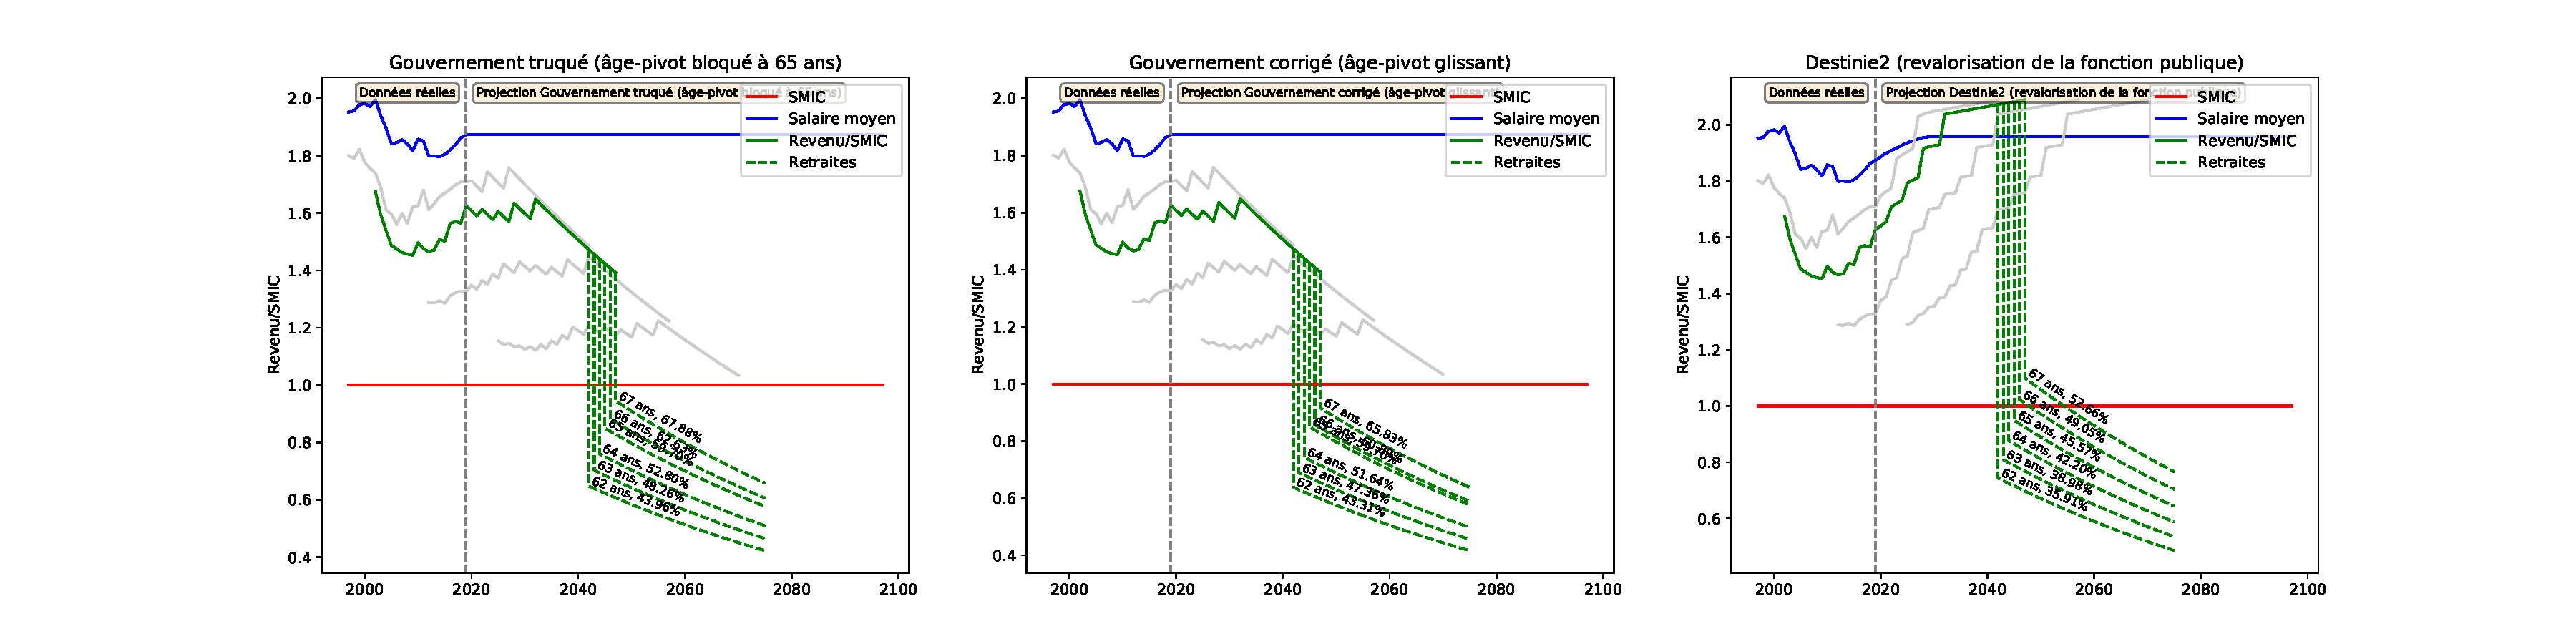
\includegraphics[width=0.9\textwidth]{fig/SecretaireAdmin_1980_22_dest_retraite.pdf}\end{center} \label{fig/SecretaireAdmin_1980_22_dest_retraite.pdf} 

\newpage 
 
\subsection{Génération 1990 (début en 2012)} 

\paragraph{Retraites possibles et ratios Revenu/SMIC à 70, 75, 80, 85, 90 ans avec le modèle \emph{Gouvernement truqué (âge-pivot bloqué à 65 ans)}}  
 
{ \scriptsize \begin{center} 
\begin{tabular}[htb]{|c|c||c|c||c|c||c||c|c|c|c|c|c|} 
\hline 
 Retraite en &  Âge &  Âge pivot &  Décote/Surcote &  Retraite (\euro{} 2019) &  Tx Rempl(\%) &  SMIC (\euro{} 2019) &  Retraite/SMIC &  Rev70/SMIC &  Rev75/SMIC &  Rev80/SMIC &  Rev85/SMIC &  Rev90/SMIC \\ 
\hline \hline 
 2052 &  62 &  65 ans 0 mois &  -15.00\% &  1587.40 &  {\bf 47.15} &  2601.14 &  {\bf {\color{red} 0.61}} &  {\bf {\color{red} 0.55}} &  {\bf {\color{red} 0.52}} &  {\bf {\color{red} 0.48}} &  {\bf {\color{red} 0.45}} &  {\bf {\color{red} 0.43}} \\ 
\hline 
 2053 &  63 &  65 ans 0 mois &  -10.00\% &  1744.88 &  {\bf 51.74} &  2634.96 &  {\bf {\color{red} 0.66}} &  {\bf {\color{red} 0.60}} &  {\bf {\color{red} 0.57}} &  {\bf {\color{red} 0.53}} &  {\bf {\color{red} 0.50}} &  {\bf {\color{red} 0.47}} \\ 
\hline 
 2054 &  64 &  65 ans 0 mois &  -5.00\% &  1910.43 &  {\bf 56.56} &  2669.21 &  {\bf {\color{red} 0.72}} &  {\bf {\color{red} 0.66}} &  {\bf {\color{red} 0.62}} &  {\bf {\color{red} 0.58}} &  {\bf {\color{red} 0.55}} &  {\bf {\color{red} 0.51}} \\ 
\hline 
 2055 &  65 &  65 ans 0 mois &  0.00\% &  2298.33 &  {\bf 67.93} &  2703.91 &  {\bf {\color{red} 0.85}} &  {\bf {\color{red} 0.80}} &  {\bf {\color{red} 0.75}} &  {\bf {\color{red} 0.70}} &  {\bf {\color{red} 0.66}} &  {\bf {\color{red} 0.62}} \\ 
\hline 
 2056 &  66 &  65 ans 0 mois &  5.00\% &  2328.20 &  {\bf 68.70} &  2739.06 &  {\bf {\color{red} 0.85}} &  {\bf {\color{red} 0.81}} &  {\bf {\color{red} 0.76}} &  {\bf {\color{red} 0.71}} &  {\bf {\color{red} 0.67}} &  {\bf {\color{red} 0.62}} \\ 
\hline 
 2057 &  67 &  65 ans 0 mois &  10.00\% &  2457.17 &  {\bf 72.39} &  2774.67 &  {\bf {\color{red} 0.89}} &  {\bf {\color{red} 0.85}} &  {\bf {\color{red} 0.80}} &  {\bf {\color{red} 0.75}} &  {\bf {\color{red} 0.70}} &  {\bf {\color{red} 0.66}} \\ 
\hline 
\hline 
\end{tabular} 
\end{center} } 
\paragraph{Retraites possibles et ratios Revenu/SMIC à 70, 75, 80, 85, 90 ans avec le modèle \emph{Gouvernement corrigé (âge-pivot glissant)}}  
 
{ \scriptsize \begin{center} 
\begin{tabular}[htb]{|c|c||c|c||c|c||c||c|c|c|c|c|c|} 
\hline 
 Retraite en &  Âge &  Âge pivot &  Décote/Surcote &  Retraite (\euro{} 2019) &  Tx Rempl(\%) &  SMIC (\euro{} 2019) &  Retraite/SMIC &  Rev70/SMIC &  Rev75/SMIC &  Rev80/SMIC &  Rev85/SMIC &  Rev90/SMIC \\ 
\hline \hline 
 2052 &  62 &  66 ans 1 mois &  -20.42\% &  1486.25 &  {\bf 44.14} &  2601.14 &  {\bf {\color{red} 0.57}} &  {\bf {\color{red} 0.52}} &  {\bf {\color{red} 0.48}} &  {\bf {\color{red} 0.45}} &  {\bf {\color{red} 0.42}} &  {\bf {\color{red} 0.40}} \\ 
\hline 
 2053 &  63 &  66 ans 2 mois &  -15.83\% &  1631.78 &  {\bf 48.39} &  2634.96 &  {\bf {\color{red} 0.62}} &  {\bf {\color{red} 0.57}} &  {\bf {\color{red} 0.53}} &  {\bf {\color{red} 0.50}} &  {\bf {\color{red} 0.47}} &  {\bf {\color{red} 0.44}} \\ 
\hline 
 2054 &  64 &  66 ans 3 mois &  -11.25\% &  1784.74 &  {\bf 52.84} &  2669.21 &  {\bf {\color{red} 0.67}} &  {\bf {\color{red} 0.62}} &  {\bf {\color{red} 0.58}} &  {\bf {\color{red} 0.54}} &  {\bf {\color{red} 0.51}} &  {\bf {\color{red} 0.48}} \\ 
\hline 
 2055 &  65 &  66 ans 4 mois &  -6.67\% &  2298.33 &  {\bf 67.93} &  2703.91 &  {\bf {\color{red} 0.85}} &  {\bf {\color{red} 0.80}} &  {\bf {\color{red} 0.75}} &  {\bf {\color{red} 0.70}} &  {\bf {\color{red} 0.66}} &  {\bf {\color{red} 0.62}} \\ 
\hline 
 2056 &  66 &  66 ans 5 mois &  -2.08\% &  2328.20 &  {\bf 68.70} &  2739.06 &  {\bf {\color{red} 0.85}} &  {\bf {\color{red} 0.81}} &  {\bf {\color{red} 0.76}} &  {\bf {\color{red} 0.71}} &  {\bf {\color{red} 0.67}} &  {\bf {\color{red} 0.62}} \\ 
\hline 
 2057 &  67 &  66 ans 6 mois &  2.50\% &  2358.47 &  {\bf 69.48} &  2774.67 &  {\bf {\color{red} 0.85}} &  {\bf {\color{red} 0.82}} &  {\bf {\color{red} 0.77}} &  {\bf {\color{red} 0.72}} &  {\bf {\color{red} 0.67}} &  {\bf {\color{red} 0.63}} \\ 
\hline 
\hline 
\end{tabular} 
\end{center} } 
\paragraph{Retraites possibles et ratios Revenu/SMIC à 70, 75, 80, 85, 90 ans avec le modèle \emph{Destinie2 (revalorisation de la fonction publique)}}  
 
{ \scriptsize \begin{center} 
\begin{tabular}[htb]{|c|c||c|c||c|c||c||c|c|c|c|c|c|} 
\hline 
 Retraite en &  Âge &  Âge pivot &  Décote/Surcote &  Retraite (\euro{} 2019) &  Tx Rempl(\%) &  SMIC (\euro{} 2019) &  Retraite/SMIC &  Rev70/SMIC &  Rev75/SMIC &  Rev80/SMIC &  Rev85/SMIC &  Rev90/SMIC \\ 
\hline \hline 
 2052 &  62 &  66 ans 1 mois &  -20.42\% &  1851.13 &  {\bf 36.35} &  2445.56 &  {\bf {\color{red} 0.76}} &  {\bf {\color{red} 0.68}} &  {\bf {\color{red} 0.64}} &  {\bf {\color{red} 0.60}} &  {\bf {\color{red} 0.56}} &  {\bf {\color{red} 0.53}} \\ 
\hline 
 2053 &  63 &  66 ans 2 mois &  -15.83\% &  2043.62 &  {\bf 39.62} &  2477.35 &  {\bf {\color{red} 0.82}} &  {\bf {\color{red} 0.75}} &  {\bf {\color{red} 0.71}} &  {\bf {\color{red} 0.66}} &  {\bf {\color{red} 0.62}} &  {\bf {\color{red} 0.58}} \\ 
\hline 
 2054 &  64 &  66 ans 3 mois &  -11.25\% &  2247.47 &  {\bf 43.01} &  2509.56 &  {\bf {\color{red} 0.90}} &  {\bf {\color{red} 0.83}} &  {\bf {\color{red} 0.78}} &  {\bf {\color{red} 0.73}} &  {\bf {\color{red} 0.68}} &  {\bf {\color{red} 0.64}} \\ 
\hline 
 2055 &  65 &  66 ans 4 mois &  -6.67\% &  2463.04 &  {\bf 46.53} &  2542.18 &  {\bf {\color{red} 0.97}} &  {\bf {\color{red} 0.91}} &  {\bf {\color{red} 0.85}} &  {\bf {\color{red} 0.80}} &  {\bf {\color{red} 0.75}} &  {\bf {\color{red} 0.70}} \\ 
\hline 
 2056 &  66 &  66 ans 5 mois &  -2.08\% &  2690.67 &  {\bf 50.18} &  2575.23 &  {\bf 1.04} &  {\bf {\color{red} 0.99}} &  {\bf {\color{red} 0.93}} &  {\bf {\color{red} 0.87}} &  {\bf {\color{red} 0.82}} &  {\bf {\color{red} 0.77}} \\ 
\hline 
 2057 &  67 &  66 ans 6 mois &  2.50\% &  2930.73 &  {\bf 53.95} &  2608.71 &  {\bf 1.12} &  {\bf 1.08} &  {\bf 1.01} &  {\bf {\color{red} 0.95}} &  {\bf {\color{red} 0.89}} &  {\bf {\color{red} 0.83}} \\ 
\hline 
\hline 
\end{tabular} 
\end{center} } 

 \begin{center}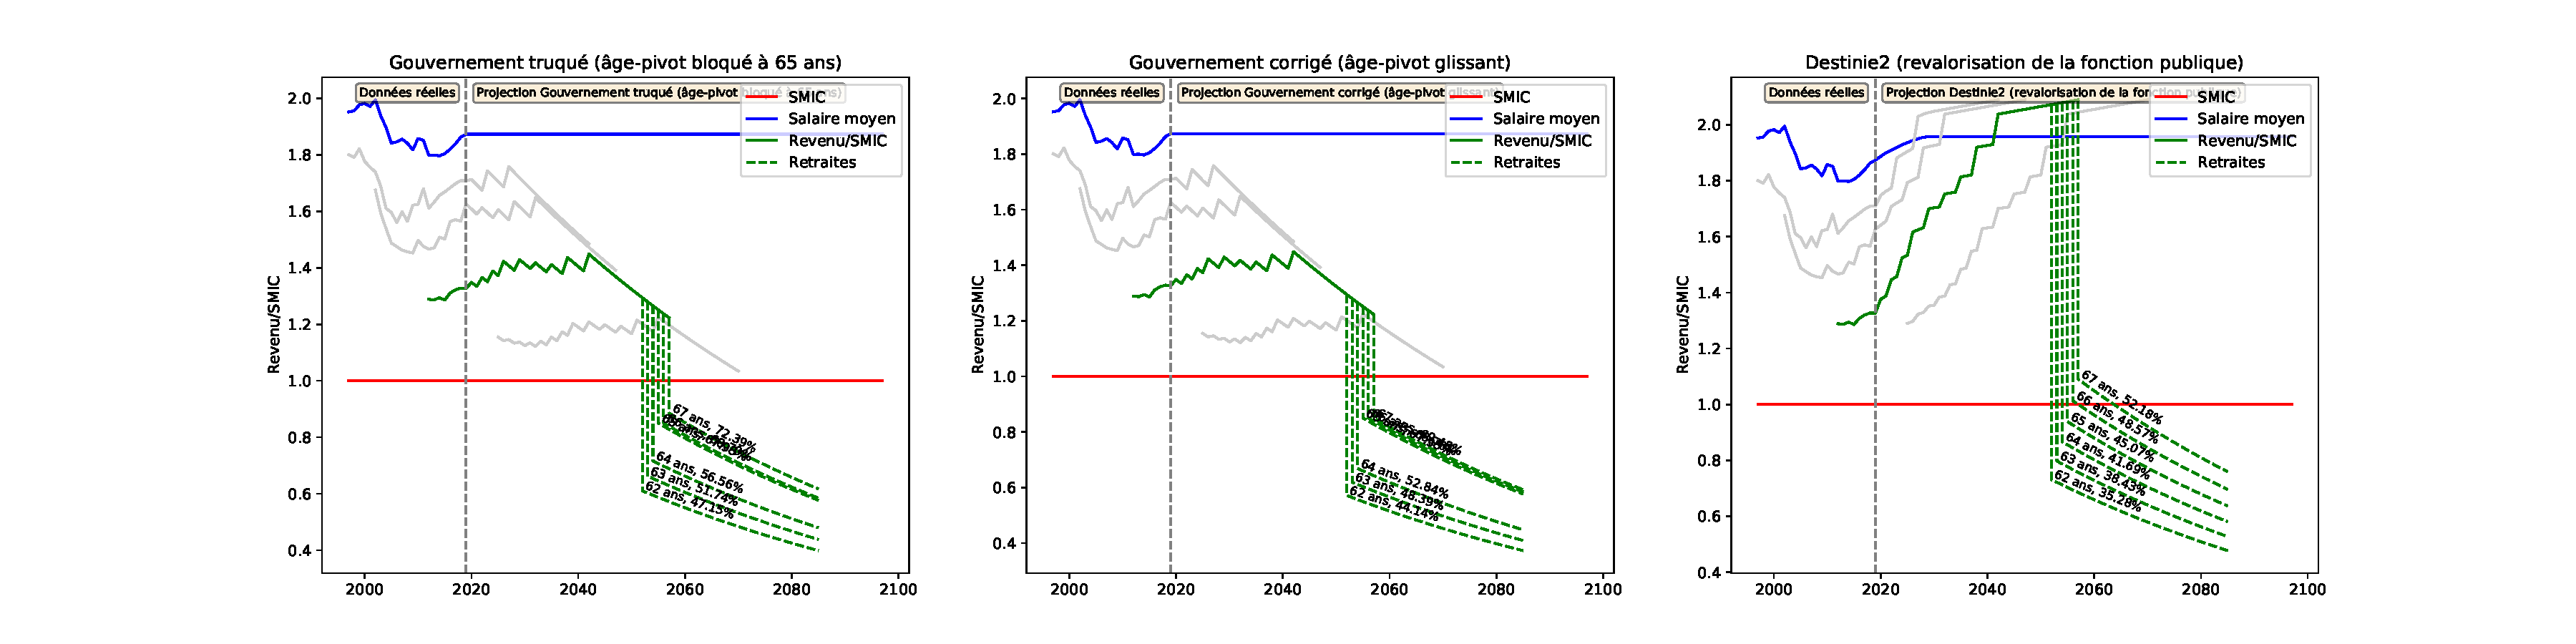
\includegraphics[width=0.9\textwidth]{fig/SecretaireAdmin_1990_22_dest_retraite.pdf}\end{center} \label{fig/SecretaireAdmin_1990_22_dest_retraite.pdf} 

\newpage 
 
\subsection{Génération 2003 (début en 2025)} 

\paragraph{Retraites possibles et ratios Revenu/SMIC à 70, 75, 80, 85, 90 ans avec le modèle \emph{Gouvernement truqué (âge-pivot bloqué à 65 ans)}}  
 
{ \scriptsize \begin{center} 
\begin{tabular}[htb]{|c|c||c|c||c|c||c||c|c|c|c|c|c|} 
\hline 
 Retraite en &  Âge &  Âge pivot &  Décote/Surcote &  Retraite (\euro{} 2019) &  Tx Rempl(\%) &  SMIC (\euro{} 2019) &  Retraite/SMIC &  Rev70/SMIC &  Rev75/SMIC &  Rev80/SMIC &  Rev85/SMIC &  Rev90/SMIC \\ 
\hline \hline 
 2065 &  62 &  65 ans 0 mois &  -15.00\% &  1698.65 &  {\bf 50.45} &  3076.71 &  {\bf {\color{red} 0.55}} &  {\bf {\color{red} 0.50}} &  {\bf {\color{red} 0.47}} &  {\bf {\color{red} 0.44}} &  {\bf {\color{red} 0.41}} &  {\bf {\color{red} 0.38}} \\ 
\hline 
 2066 &  63 &  65 ans 0 mois &  -10.00\% &  1864.20 &  {\bf 55.28} &  3116.71 &  {\bf {\color{red} 0.60}} &  {\bf {\color{red} 0.55}} &  {\bf {\color{red} 0.51}} &  {\bf {\color{red} 0.48}} &  {\bf {\color{red} 0.45}} &  {\bf {\color{red} 0.42}} \\ 
\hline 
 2067 &  64 &  65 ans 0 mois &  -5.00\% &  2038.01 &  {\bf 60.33} &  3157.23 &  {\bf {\color{red} 0.65}} &  {\bf {\color{red} 0.60}} &  {\bf {\color{red} 0.56}} &  {\bf {\color{red} 0.52}} &  {\bf {\color{red} 0.49}} &  {\bf {\color{red} 0.46}} \\ 
\hline 
 2068 &  65 &  65 ans 0 mois &  0.00\% &  2718.53 &  {\bf 80.35} &  3198.27 &  {\bf {\color{red} 0.85}} &  {\bf {\color{red} 0.80}} &  {\bf {\color{red} 0.75}} &  {\bf {\color{red} 0.70}} &  {\bf {\color{red} 0.66}} &  {\bf {\color{red} 0.62}} \\ 
\hline 
 2069 &  66 &  65 ans 0 mois &  5.00\% &  2753.87 &  {\bf 81.26} &  3239.85 &  {\bf {\color{red} 0.85}} &  {\bf {\color{red} 0.81}} &  {\bf {\color{red} 0.76}} &  {\bf {\color{red} 0.71}} &  {\bf {\color{red} 0.67}} &  {\bf {\color{red} 0.62}} \\ 
\hline 
 2070 &  67 &  65 ans 0 mois &  10.00\% &  2789.67 &  {\bf 82.18} &  3281.97 &  {\bf {\color{red} 0.85}} &  {\bf {\color{red} 0.82}} &  {\bf {\color{red} 0.77}} &  {\bf {\color{red} 0.72}} &  {\bf {\color{red} 0.67}} &  {\bf {\color{red} 0.63}} \\ 
\hline 
\hline 
\end{tabular} 
\end{center} } 
\paragraph{Retraites possibles et ratios Revenu/SMIC à 70, 75, 80, 85, 90 ans avec le modèle \emph{Gouvernement corrigé (âge-pivot glissant)}}  
 
{ \scriptsize \begin{center} 
\begin{tabular}[htb]{|c|c||c|c||c|c||c||c|c|c|c|c|c|} 
\hline 
 Retraite en &  Âge &  Âge pivot &  Décote/Surcote &  Retraite (\euro{} 2019) &  Tx Rempl(\%) &  SMIC (\euro{} 2019) &  Retraite/SMIC &  Rev70/SMIC &  Rev75/SMIC &  Rev80/SMIC &  Rev85/SMIC &  Rev90/SMIC \\ 
\hline \hline 
 2065 &  62 &  67 ans 2 mois &  -25.83\% &  1482.15 &  {\bf 44.02} &  3076.71 &  {\bf {\color{red} 0.48}} &  {\bf {\color{red} 0.43}} &  {\bf {\color{red} 0.41}} &  {\bf {\color{red} 0.38}} &  {\bf {\color{red} 0.36}} &  {\bf {\color{red} 0.34}} \\ 
\hline 
 2066 &  63 &  67 ans 3 mois &  -21.25\% &  1631.17 &  {\bf 48.37} &  3116.71 &  {\bf {\color{red} 0.52}} &  {\bf {\color{red} 0.48}} &  {\bf {\color{red} 0.45}} &  {\bf {\color{red} 0.42}} &  {\bf {\color{red} 0.39}} &  {\bf {\color{red} 0.37}} \\ 
\hline 
 2067 &  64 &  67 ans 4 mois &  -16.67\% &  1787.73 &  {\bf 52.92} &  3157.23 &  {\bf {\color{red} 0.57}} &  {\bf {\color{red} 0.52}} &  {\bf {\color{red} 0.49}} &  {\bf {\color{red} 0.46}} &  {\bf {\color{red} 0.43}} &  {\bf {\color{red} 0.40}} \\ 
\hline 
 2068 &  65 &  67 ans 5 mois &  -12.08\% &  2718.53 &  {\bf 80.35} &  3198.27 &  {\bf {\color{red} 0.85}} &  {\bf {\color{red} 0.80}} &  {\bf {\color{red} 0.75}} &  {\bf {\color{red} 0.70}} &  {\bf {\color{red} 0.66}} &  {\bf {\color{red} 0.62}} \\ 
\hline 
 2069 &  66 &  67 ans 6 mois &  -7.50\% &  2753.87 &  {\bf 81.26} &  3239.85 &  {\bf {\color{red} 0.85}} &  {\bf {\color{red} 0.81}} &  {\bf {\color{red} 0.76}} &  {\bf {\color{red} 0.71}} &  {\bf {\color{red} 0.67}} &  {\bf {\color{red} 0.62}} \\ 
\hline 
 2070 &  67 &  67 ans 7 mois &  -2.92\% &  2789.67 &  {\bf 82.18} &  3281.97 &  {\bf {\color{red} 0.85}} &  {\bf {\color{red} 0.82}} &  {\bf {\color{red} 0.77}} &  {\bf {\color{red} 0.72}} &  {\bf {\color{red} 0.67}} &  {\bf {\color{red} 0.63}} \\ 
\hline 
\hline 
\end{tabular} 
\end{center} } 
\paragraph{Retraites possibles et ratios Revenu/SMIC à 70, 75, 80, 85, 90 ans avec le modèle \emph{Destinie2 (revalorisation de la fonction publique)}}  
 
{ \scriptsize \begin{center} 
\begin{tabular}[htb]{|c|c||c|c||c|c||c||c|c|c|c|c|c|} 
\hline 
 Retraite en &  Âge &  Âge pivot &  Décote/Surcote &  Retraite (\euro{} 2019) &  Tx Rempl(\%) &  SMIC (\euro{} 2019) &  Retraite/SMIC &  Rev70/SMIC &  Rev75/SMIC &  Rev80/SMIC &  Rev85/SMIC &  Rev90/SMIC \\ 
\hline \hline 
 2065 &  62 &  67 ans 2 mois &  -25.83\% &  2146.37 &  {\bf 35.63} &  2892.68 &  {\bf {\color{red} 0.74}} &  {\bf {\color{red} 0.67}} &  {\bf {\color{red} 0.63}} &  {\bf {\color{red} 0.59}} &  {\bf {\color{red} 0.55}} &  {\bf {\color{red} 0.52}} \\ 
\hline 
 2066 &  63 &  67 ans 3 mois &  -21.25\% &  2375.52 &  {\bf 38.93} &  2930.29 &  {\bf {\color{red} 0.81}} &  {\bf {\color{red} 0.74}} &  {\bf {\color{red} 0.69}} &  {\bf {\color{red} 0.65}} &  {\bf {\color{red} 0.61}} &  {\bf {\color{red} 0.57}} \\ 
\hline 
 2067 &  64 &  67 ans 4 mois &  -16.67\% &  2618.15 &  {\bf 42.36} &  2968.38 &  {\bf {\color{red} 0.88}} &  {\bf {\color{red} 0.82}} &  {\bf {\color{red} 0.77}} &  {\bf {\color{red} 0.72}} &  {\bf {\color{red} 0.67}} &  {\bf {\color{red} 0.63}} \\ 
\hline 
 2068 &  65 &  67 ans 5 mois &  -12.08\% &  2874.68 &  {\bf 45.91} &  3006.97 &  {\bf {\color{red} 0.96}} &  {\bf {\color{red} 0.90}} &  {\bf {\color{red} 0.84}} &  {\bf {\color{red} 0.79}} &  {\bf {\color{red} 0.74}} &  {\bf {\color{red} 0.69}} \\ 
\hline 
 2069 &  66 &  67 ans 6 mois &  -7.50\% &  3145.53 &  {\bf 49.59} &  3046.06 &  {\bf 1.03} &  {\bf {\color{red} 0.98}} &  {\bf {\color{red} 0.92}} &  {\bf {\color{red} 0.86}} &  {\bf {\color{red} 0.81}} &  {\bf {\color{red} 0.76}} \\ 
\hline 
 2070 &  67 &  67 ans 7 mois &  -2.92\% &  3431.13 &  {\bf 53.40} &  3085.66 &  {\bf 1.11} &  {\bf 1.07} &  {\bf 1.00} &  {\bf {\color{red} 0.94}} &  {\bf {\color{red} 0.88}} &  {\bf {\color{red} 0.83}} \\ 
\hline 
\hline 
\end{tabular} 
\end{center} } 

 \begin{center}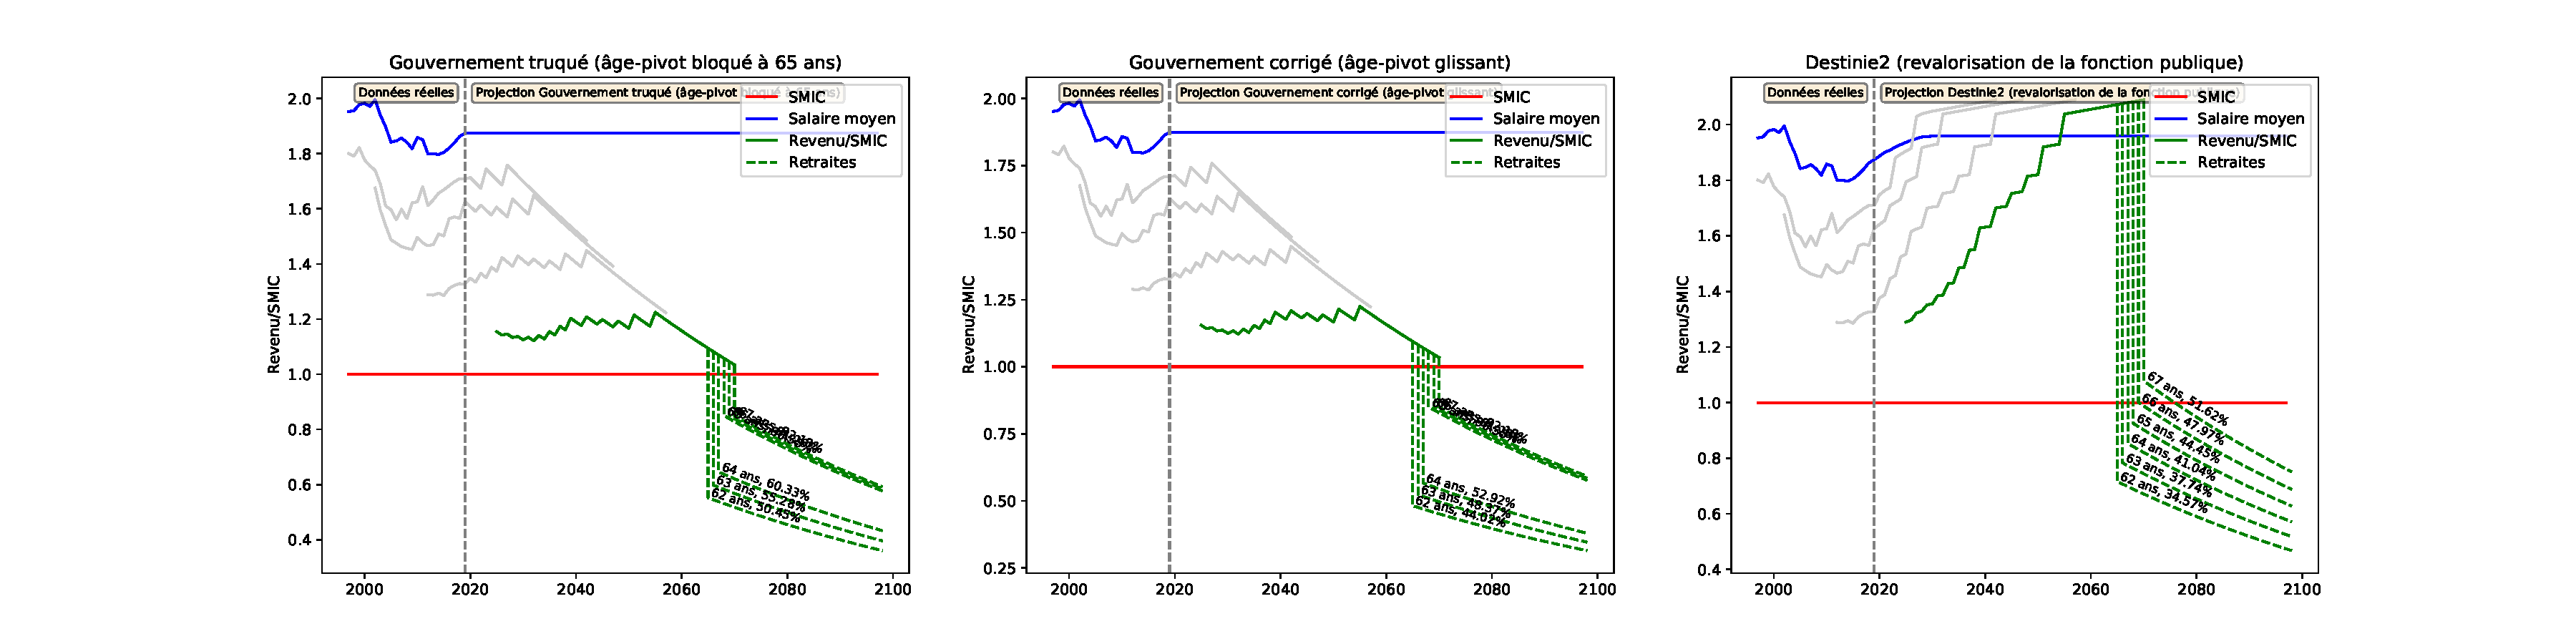
\includegraphics[width=0.9\textwidth]{fig/SecretaireAdmin_2003_22_dest_retraite.pdf}\end{center} \label{fig/SecretaireAdmin_2003_22_dest_retraite.pdf} 

\newpage 
 
\chapter{ATSEM (C2 puis C1)} 

\begin{minipage}{0.55\linewidth}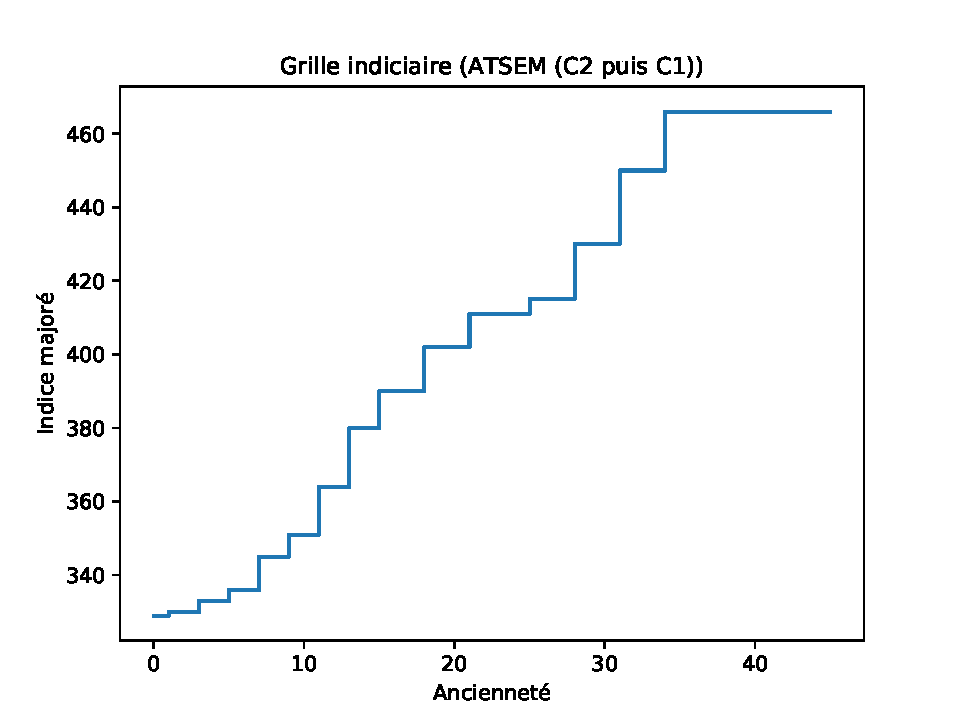
\includegraphics[width=0.7\textwidth]{fig/grille_ATSEM.pdf}\end{minipage} 
\begin{minipage}{0.3\linewidth} 
 \begin{center} 

\begin{tabular}[htb]{|c|c|} 
\hline 
 Indice majoré &  Durée (années) \\ 
\hline \hline 
 329 &  1.00 \\ 
\hline 
 330 &  2.00 \\ 
\hline 
 333 &  2.00 \\ 
\hline 
 336 &  2.00 \\ 
\hline 
 345 &  2.00 \\ 
\hline 
 351 &  2.00 \\ 
\hline 
 364 &  2.00 \\ 
\hline 
 380 &  2.00 \\ 
\hline 
 390 &  3.00 \\ 
\hline 
 402 &  3.00 \\ 
\hline 
 411 &  4.00 \\ 
\hline 
 415 &  3.00 \\ 
\hline 
 430 &  3.00 \\ 
\hline 
 450 &  3.00 \\ 
\hline 
 466 &   \\ 
\hline 
\hline 
\end{tabular} 
\end{center} 
 \end{minipage} 


 \addto{\captionsenglish}{ \renewcommand{\mtctitle}{}} \setcounter{minitocdepth}{2} 
 \minitoc \newpage 

\section{Début de carrière à 22 ans} 

\subsection{Génération 1975 (début en 1997)} 

\paragraph{Retraites possibles et ratios Revenu/SMIC à 70, 75, 80, 85, 90 ans avec le modèle \emph{Gouvernement truqué (âge-pivot bloqué à 65 ans)}}  
 
{ \scriptsize \begin{center} 
\begin{tabular}[htb]{|c|c||c|c||c|c||c||c|c|c|c|c|c|} 
\hline 
 Retraite en &  Âge &  Âge pivot &  Décote/Surcote &  Retraite (\euro{} 2019) &  Tx Rempl(\%) &  SMIC (\euro{} 2019) &  Retraite/SMIC &  Rev70/SMIC &  Rev75/SMIC &  Rev80/SMIC &  Rev85/SMIC &  Rev90/SMIC \\ 
\hline \hline 
 2037 &  62 &  64 ans 10 mois &  -14.17\% &  1115.00 &  {\bf 43.28} &  2143.00 &  {\bf {\color{red} 0.52}} &  {\bf {\color{red} 0.47}} &  {\bf {\color{red} 0.44}} &  {\bf {\color{red} 0.41}} &  {\bf {\color{red} 0.39}} &  {\bf {\color{red} 0.36}} \\ 
\hline 
 2038 &  63 &  64 ans 11 mois &  -9.58\% &  1215.99 &  {\bf 47.11} &  2170.86 &  {\bf {\color{red} 0.56}} &  {\bf {\color{red} 0.51}} &  {\bf {\color{red} 0.48}} &  {\bf {\color{red} 0.45}} &  {\bf {\color{red} 0.42}} &  {\bf {\color{red} 0.40}} \\ 
\hline 
 2039 &  64 &  65 ans 0 mois &  -5.00\% &  1322.55 &  {\bf 51.13} &  2199.08 &  {\bf {\color{red} 0.60}} &  {\bf {\color{red} 0.56}} &  {\bf {\color{red} 0.52}} &  {\bf {\color{red} 0.49}} &  {\bf {\color{red} 0.46}} &  {\bf {\color{red} 0.43}} \\ 
\hline 
 2040 &  65 &  65 ans 0 mois &  0.00\% &  1893.52 &  {\bf 73.06} &  2227.67 &  {\bf {\color{red} 0.85}} &  {\bf {\color{red} 0.80}} &  {\bf {\color{red} 0.75}} &  {\bf {\color{red} 0.70}} &  {\bf {\color{red} 0.66}} &  {\bf {\color{red} 0.62}} \\ 
\hline 
 2041 &  66 &  65 ans 0 mois &  5.00\% &  1918.14 &  {\bf 73.87} &  2256.63 &  {\bf {\color{red} 0.85}} &  {\bf {\color{red} 0.81}} &  {\bf {\color{red} 0.76}} &  {\bf {\color{red} 0.71}} &  {\bf {\color{red} 0.67}} &  {\bf {\color{red} 0.62}} \\ 
\hline 
 2042 &  67 &  65 ans 0 mois &  10.00\% &  1943.07 &  {\bf 74.68} &  2285.97 &  {\bf {\color{red} 0.85}} &  {\bf {\color{red} 0.82}} &  {\bf {\color{red} 0.77}} &  {\bf {\color{red} 0.72}} &  {\bf {\color{red} 0.67}} &  {\bf {\color{red} 0.63}} \\ 
\hline 
\hline 
\end{tabular} 
\end{center} } 
\paragraph{Retraites possibles et ratios Revenu/SMIC à 70, 75, 80, 85, 90 ans avec le modèle \emph{Gouvernement corrigé (âge-pivot glissant)}}  
 
{ \scriptsize \begin{center} 
\begin{tabular}[htb]{|c|c||c|c||c|c||c||c|c|c|c|c|c|} 
\hline 
 Retraite en &  Âge &  Âge pivot &  Décote/Surcote &  Retraite (\euro{} 2019) &  Tx Rempl(\%) &  SMIC (\euro{} 2019) &  Retraite/SMIC &  Rev70/SMIC &  Rev75/SMIC &  Rev80/SMIC &  Rev85/SMIC &  Rev90/SMIC \\ 
\hline \hline 
 2037 &  62 &  64 ans 10 mois &  -14.17\% &  1115.00 &  {\bf 43.28} &  2143.00 &  {\bf {\color{red} 0.52}} &  {\bf {\color{red} 0.47}} &  {\bf {\color{red} 0.44}} &  {\bf {\color{red} 0.41}} &  {\bf {\color{red} 0.39}} &  {\bf {\color{red} 0.36}} \\ 
\hline 
 2038 &  63 &  64 ans 11 mois &  -9.58\% &  1215.99 &  {\bf 47.11} &  2170.86 &  {\bf {\color{red} 0.56}} &  {\bf {\color{red} 0.51}} &  {\bf {\color{red} 0.48}} &  {\bf {\color{red} 0.45}} &  {\bf {\color{red} 0.42}} &  {\bf {\color{red} 0.40}} \\ 
\hline 
 2039 &  64 &  65 ans 0 mois &  -5.00\% &  1322.55 &  {\bf 51.13} &  2199.08 &  {\bf {\color{red} 0.60}} &  {\bf {\color{red} 0.56}} &  {\bf {\color{red} 0.52}} &  {\bf {\color{red} 0.49}} &  {\bf {\color{red} 0.46}} &  {\bf {\color{red} 0.43}} \\ 
\hline 
 2040 &  65 &  65 ans 1 mois &  -0.42\% &  1893.52 &  {\bf 73.06} &  2227.67 &  {\bf {\color{red} 0.85}} &  {\bf {\color{red} 0.80}} &  {\bf {\color{red} 0.75}} &  {\bf {\color{red} 0.70}} &  {\bf {\color{red} 0.66}} &  {\bf {\color{red} 0.62}} \\ 
\hline 
 2041 &  66 &  65 ans 2 mois &  4.17\% &  1918.14 &  {\bf 73.87} &  2256.63 &  {\bf {\color{red} 0.85}} &  {\bf {\color{red} 0.81}} &  {\bf {\color{red} 0.76}} &  {\bf {\color{red} 0.71}} &  {\bf {\color{red} 0.67}} &  {\bf {\color{red} 0.62}} \\ 
\hline 
 2042 &  67 &  65 ans 3 mois &  8.75\% &  1943.07 &  {\bf 74.68} &  2285.97 &  {\bf {\color{red} 0.85}} &  {\bf {\color{red} 0.82}} &  {\bf {\color{red} 0.77}} &  {\bf {\color{red} 0.72}} &  {\bf {\color{red} 0.67}} &  {\bf {\color{red} 0.63}} \\ 
\hline 
\hline 
\end{tabular} 
\end{center} } 
\paragraph{Retraites possibles et ratios Revenu/SMIC à 70, 75, 80, 85, 90 ans avec le modèle \emph{Destinie2 (revalorisation de la fonction publique)}}  
 
{ \scriptsize \begin{center} 
\begin{tabular}[htb]{|c|c||c|c||c|c||c||c|c|c|c|c|c|} 
\hline 
 Retraite en &  Âge &  Âge pivot &  Décote/Surcote &  Retraite (\euro{} 2019) &  Tx Rempl(\%) &  SMIC (\euro{} 2019) &  Retraite/SMIC &  Rev70/SMIC &  Rev75/SMIC &  Rev80/SMIC &  Rev85/SMIC &  Rev90/SMIC \\ 
\hline \hline 
 2037 &  62 &  64 ans 10 mois &  -14.17\% &  1234.07 &  {\bf 38.40} &  2014.82 &  {\bf {\color{red} 0.61}} &  {\bf {\color{red} 0.55}} &  {\bf {\color{red} 0.52}} &  {\bf {\color{red} 0.49}} &  {\bf {\color{red} 0.46}} &  {\bf {\color{red} 0.43}} \\ 
\hline 
 2038 &  63 &  64 ans 11 mois &  -9.58\% &  1350.85 &  {\bf 41.50} &  2041.01 &  {\bf {\color{red} 0.66}} &  {\bf {\color{red} 0.60}} &  {\bf {\color{red} 0.57}} &  {\bf {\color{red} 0.53}} &  {\bf {\color{red} 0.50}} &  {\bf {\color{red} 0.47}} \\ 
\hline 
 2039 &  64 &  65 ans 0 mois &  -5.00\% &  1474.85 &  {\bf 44.72} &  2067.55 &  {\bf {\color{red} 0.71}} &  {\bf {\color{red} 0.66}} &  {\bf {\color{red} 0.62}} &  {\bf {\color{red} 0.58}} &  {\bf {\color{red} 0.54}} &  {\bf {\color{red} 0.51}} \\ 
\hline 
 2040 &  65 &  65 ans 1 mois &  -0.42\% &  1780.26 &  {\bf 53.29} &  2094.43 &  {\bf {\color{red} 0.85}} &  {\bf {\color{red} 0.80}} &  {\bf {\color{red} 0.75}} &  {\bf {\color{red} 0.70}} &  {\bf {\color{red} 0.66}} &  {\bf {\color{red} 0.62}} \\ 
\hline 
 2041 &  66 &  65 ans 2 mois &  4.17\% &  1803.40 &  {\bf 53.29} &  2121.65 &  {\bf {\color{red} 0.85}} &  {\bf {\color{red} 0.81}} &  {\bf {\color{red} 0.76}} &  {\bf {\color{red} 0.71}} &  {\bf {\color{red} 0.67}} &  {\bf {\color{red} 0.62}} \\ 
\hline 
 2042 &  67 &  65 ans 3 mois &  8.75\% &  1894.37 &  {\bf 55.26} &  2149.23 &  {\bf {\color{red} 0.88}} &  {\bf {\color{red} 0.85}} &  {\bf {\color{red} 0.79}} &  {\bf {\color{red} 0.75}} &  {\bf {\color{red} 0.70}} &  {\bf {\color{red} 0.65}} \\ 
\hline 
\hline 
\end{tabular} 
\end{center} } 

 \begin{center}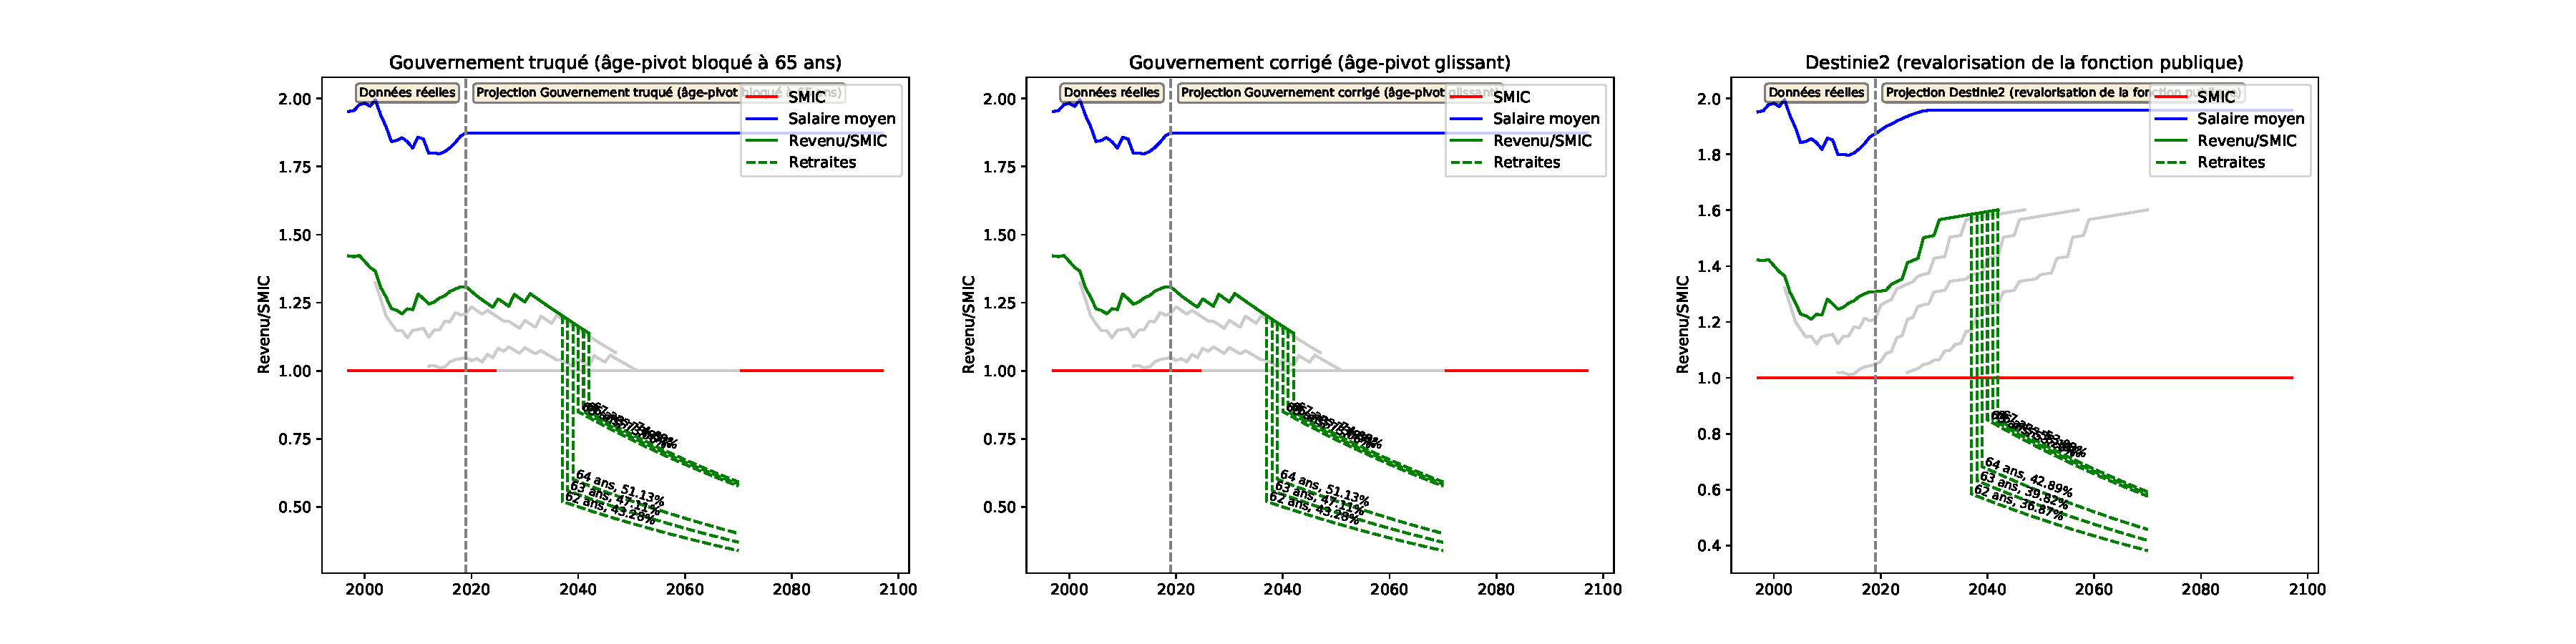
\includegraphics[width=0.9\textwidth]{fig/ATSEM_1975_22_dest_retraite.pdf}\end{center} \label{fig/ATSEM_1975_22_dest_retraite.pdf} 

\newpage 
 
\subsection{Génération 1980 (début en 2002)} 

\paragraph{Retraites possibles et ratios Revenu/SMIC à 70, 75, 80, 85, 90 ans avec le modèle \emph{Gouvernement truqué (âge-pivot bloqué à 65 ans)}}  
 
{ \scriptsize \begin{center} 
\begin{tabular}[htb]{|c|c||c|c||c|c||c||c|c|c|c|c|c|} 
\hline 
 Retraite en &  Âge &  Âge pivot &  Décote/Surcote &  Retraite (\euro{} 2019) &  Tx Rempl(\%) &  SMIC (\euro{} 2019) &  Retraite/SMIC &  Rev70/SMIC &  Rev75/SMIC &  Rev80/SMIC &  Rev85/SMIC &  Rev90/SMIC \\ 
\hline \hline 
 2042 &  62 &  65 ans 0 mois &  -15.00\% &  1123.83 &  {\bf 43.62} &  2285.97 &  {\bf {\color{red} 0.49}} &  {\bf {\color{red} 0.44}} &  {\bf {\color{red} 0.42}} &  {\bf {\color{red} 0.39}} &  {\bf {\color{red} 0.37}} &  {\bf {\color{red} 0.34}} \\ 
\hline 
 2043 &  63 &  65 ans 0 mois &  -10.00\% &  1235.91 &  {\bf 47.88} &  2315.68 &  {\bf {\color{red} 0.53}} &  {\bf {\color{red} 0.49}} &  {\bf {\color{red} 0.46}} &  {\bf {\color{red} 0.43}} &  {\bf {\color{red} 0.40}} &  {\bf {\color{red} 0.38}} \\ 
\hline 
 2044 &  64 &  65 ans 0 mois &  -5.00\% &  1354.73 &  {\bf 52.38} &  2345.79 &  {\bf {\color{red} 0.58}} &  {\bf {\color{red} 0.53}} &  {\bf {\color{red} 0.50}} &  {\bf {\color{red} 0.47}} &  {\bf {\color{red} 0.44}} &  {\bf {\color{red} 0.41}} \\ 
\hline 
 2045 &  65 &  65 ans 0 mois &  0.00\% &  2019.84 &  {\bf 77.94} &  2376.28 &  {\bf {\color{red} 0.85}} &  {\bf {\color{red} 0.80}} &  {\bf {\color{red} 0.75}} &  {\bf {\color{red} 0.70}} &  {\bf {\color{red} 0.66}} &  {\bf {\color{red} 0.62}} \\ 
\hline 
 2046 &  66 &  65 ans 0 mois &  5.00\% &  2046.10 &  {\bf 78.79} &  2407.18 &  {\bf {\color{red} 0.85}} &  {\bf {\color{red} 0.81}} &  {\bf {\color{red} 0.76}} &  {\bf {\color{red} 0.71}} &  {\bf {\color{red} 0.67}} &  {\bf {\color{red} 0.62}} \\ 
\hline 
 2047 &  67 &  65 ans 0 mois &  10.00\% &  2072.70 &  {\bf 79.66} &  2438.47 &  {\bf {\color{red} 0.85}} &  {\bf {\color{red} 0.82}} &  {\bf {\color{red} 0.77}} &  {\bf {\color{red} 0.72}} &  {\bf {\color{red} 0.67}} &  {\bf {\color{red} 0.63}} \\ 
\hline 
\hline 
\end{tabular} 
\end{center} } 
\paragraph{Retraites possibles et ratios Revenu/SMIC à 70, 75, 80, 85, 90 ans avec le modèle \emph{Gouvernement corrigé (âge-pivot glissant)}}  
 
{ \scriptsize \begin{center} 
\begin{tabular}[htb]{|c|c||c|c||c|c||c||c|c|c|c|c|c|} 
\hline 
 Retraite en &  Âge &  Âge pivot &  Décote/Surcote &  Retraite (\euro{} 2019) &  Tx Rempl(\%) &  SMIC (\euro{} 2019) &  Retraite/SMIC &  Rev70/SMIC &  Rev75/SMIC &  Rev80/SMIC &  Rev85/SMIC &  Rev90/SMIC \\ 
\hline \hline 
 2042 &  62 &  65 ans 3 mois &  -16.25\% &  1107.30 &  {\bf 42.98} &  2285.97 &  {\bf {\color{red} 0.48}} &  {\bf {\color{red} 0.44}} &  {\bf {\color{red} 0.41}} &  {\bf {\color{red} 0.38}} &  {\bf {\color{red} 0.36}} &  {\bf {\color{red} 0.34}} \\ 
\hline 
 2043 &  63 &  65 ans 4 mois &  -11.67\% &  1213.03 &  {\bf 46.99} &  2315.68 &  {\bf {\color{red} 0.52}} &  {\bf {\color{red} 0.48}} &  {\bf {\color{red} 0.45}} &  {\bf {\color{red} 0.42}} &  {\bf {\color{red} 0.39}} &  {\bf {\color{red} 0.37}} \\ 
\hline 
 2044 &  64 &  65 ans 5 mois &  -7.08\% &  1325.02 &  {\bf 51.23} &  2345.79 &  {\bf {\color{red} 0.56}} &  {\bf {\color{red} 0.52}} &  {\bf {\color{red} 0.49}} &  {\bf {\color{red} 0.46}} &  {\bf {\color{red} 0.43}} &  {\bf {\color{red} 0.40}} \\ 
\hline 
 2045 &  65 &  65 ans 6 mois &  -2.50\% &  2019.84 &  {\bf 77.94} &  2376.28 &  {\bf {\color{red} 0.85}} &  {\bf {\color{red} 0.80}} &  {\bf {\color{red} 0.75}} &  {\bf {\color{red} 0.70}} &  {\bf {\color{red} 0.66}} &  {\bf {\color{red} 0.62}} \\ 
\hline 
 2046 &  66 &  65 ans 7 mois &  2.08\% &  2046.10 &  {\bf 78.79} &  2407.18 &  {\bf {\color{red} 0.85}} &  {\bf {\color{red} 0.81}} &  {\bf {\color{red} 0.76}} &  {\bf {\color{red} 0.71}} &  {\bf {\color{red} 0.67}} &  {\bf {\color{red} 0.62}} \\ 
\hline 
 2047 &  67 &  65 ans 8 mois &  6.67\% &  2072.70 &  {\bf 79.66} &  2438.47 &  {\bf {\color{red} 0.85}} &  {\bf {\color{red} 0.82}} &  {\bf {\color{red} 0.77}} &  {\bf {\color{red} 0.72}} &  {\bf {\color{red} 0.67}} &  {\bf {\color{red} 0.63}} \\ 
\hline 
\hline 
\end{tabular} 
\end{center} } 
\paragraph{Retraites possibles et ratios Revenu/SMIC à 70, 75, 80, 85, 90 ans avec le modèle \emph{Destinie2 (revalorisation de la fonction publique)}}  
 
{ \scriptsize \begin{center} 
\begin{tabular}[htb]{|c|c||c|c||c|c||c||c|c|c|c|c|c|} 
\hline 
 Retraite en &  Âge &  Âge pivot &  Décote/Surcote &  Retraite (\euro{} 2019) &  Tx Rempl(\%) &  SMIC (\euro{} 2019) &  Retraite/SMIC &  Rev70/SMIC &  Rev75/SMIC &  Rev80/SMIC &  Rev85/SMIC &  Rev90/SMIC \\ 
\hline \hline 
 2042 &  62 &  65 ans 3 mois &  -16.25\% &  1267.25 &  {\bf 36.97} &  2149.23 &  {\bf {\color{red} 0.59}} &  {\bf {\color{red} 0.53}} &  {\bf {\color{red} 0.50}} &  {\bf {\color{red} 0.47}} &  {\bf {\color{red} 0.44}} &  {\bf {\color{red} 0.41}} \\ 
\hline 
 2043 &  63 &  65 ans 4 mois &  -11.67\% &  1394.61 &  {\bf 40.16} &  2177.17 &  {\bf {\color{red} 0.64}} &  {\bf {\color{red} 0.59}} &  {\bf {\color{red} 0.55}} &  {\bf {\color{red} 0.51}} &  {\bf {\color{red} 0.48}} &  {\bf {\color{red} 0.45}} \\ 
\hline 
 2044 &  64 &  65 ans 5 mois &  -7.08\% &  1530.41 &  {\bf 43.51} &  2205.48 &  {\bf {\color{red} 0.69}} &  {\bf {\color{red} 0.64}} &  {\bf {\color{red} 0.60}} &  {\bf {\color{red} 0.56}} &  {\bf {\color{red} 0.53}} &  {\bf {\color{red} 0.50}} \\ 
\hline 
 2045 &  65 &  65 ans 6 mois &  -2.50\% &  1899.03 &  {\bf 53.29} &  2234.15 &  {\bf {\color{red} 0.85}} &  {\bf {\color{red} 0.80}} &  {\bf {\color{red} 0.75}} &  {\bf {\color{red} 0.70}} &  {\bf {\color{red} 0.66}} &  {\bf {\color{red} 0.62}} \\ 
\hline 
 2046 &  66 &  65 ans 7 mois &  2.08\% &  1923.71 &  {\bf 53.29} &  2263.19 &  {\bf {\color{red} 0.85}} &  {\bf {\color{red} 0.81}} &  {\bf {\color{red} 0.76}} &  {\bf {\color{red} 0.71}} &  {\bf {\color{red} 0.67}} &  {\bf {\color{red} 0.62}} \\ 
\hline 
 2047 &  67 &  65 ans 8 mois &  6.67\% &  1989.18 &  {\bf 54.40} &  2292.61 &  {\bf {\color{red} 0.87}} &  {\bf {\color{red} 0.83}} &  {\bf {\color{red} 0.78}} &  {\bf {\color{red} 0.73}} &  {\bf {\color{red} 0.69}} &  {\bf {\color{red} 0.64}} \\ 
\hline 
\hline 
\end{tabular} 
\end{center} } 

 \begin{center}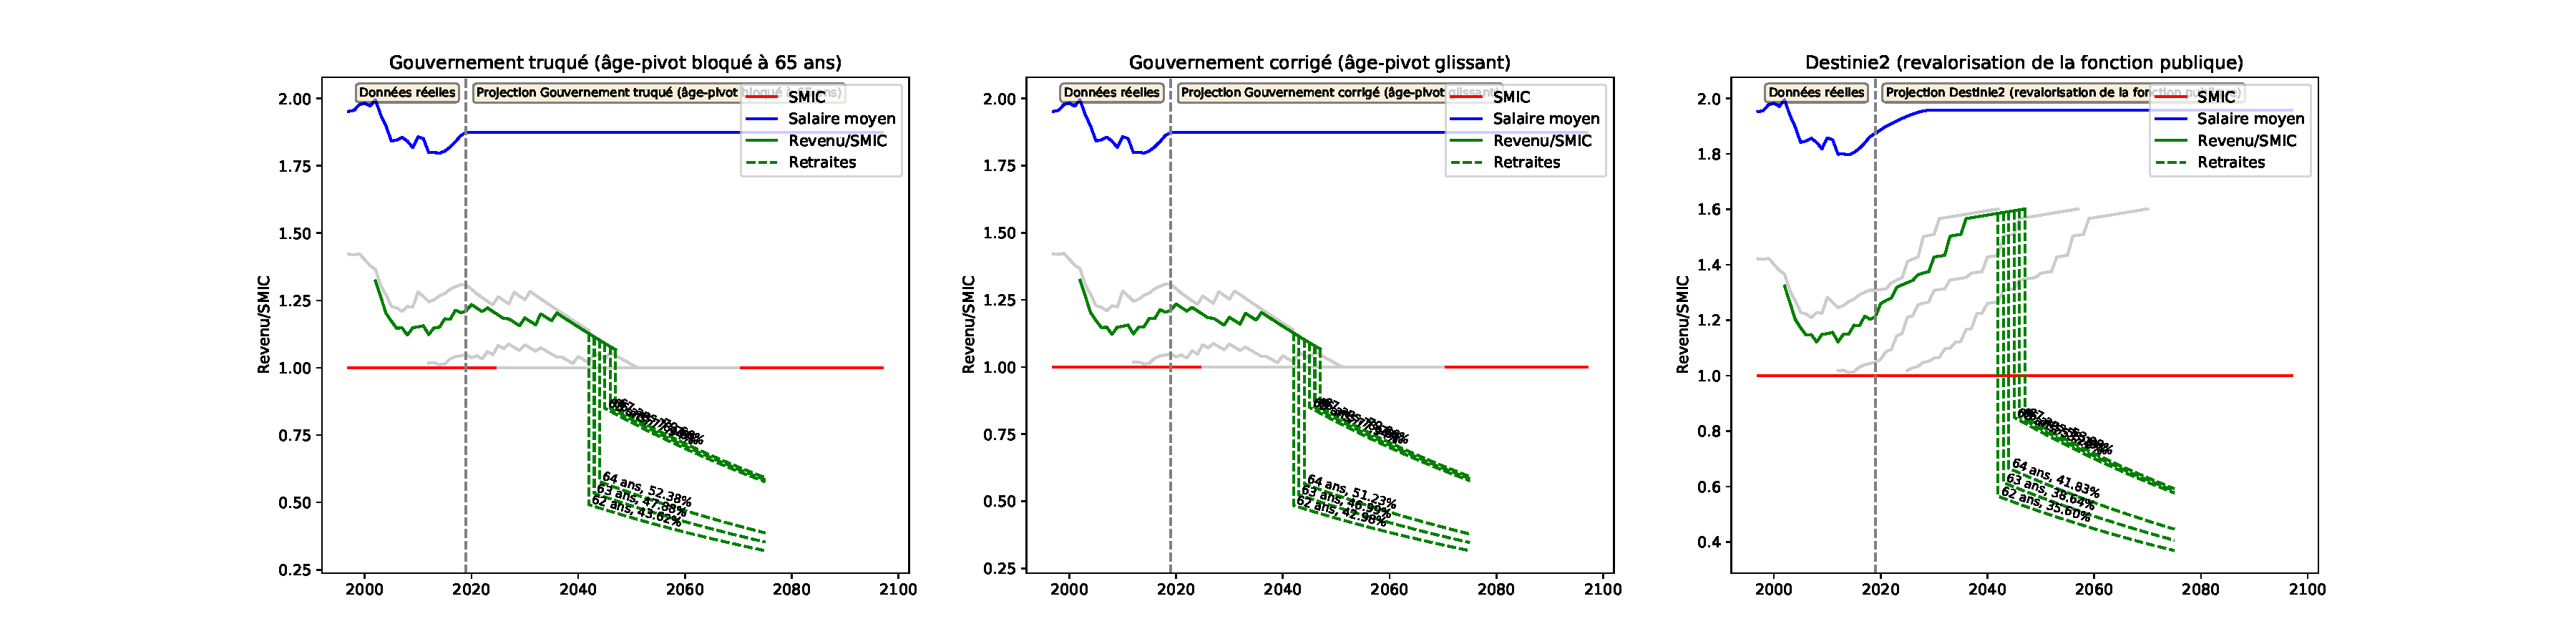
\includegraphics[width=0.9\textwidth]{fig/ATSEM_1980_22_dest_retraite.pdf}\end{center} \label{fig/ATSEM_1980_22_dest_retraite.pdf} 

\newpage 
 
\subsection{Génération 1990 (début en 2012)} 

\paragraph{Retraites possibles et ratios Revenu/SMIC à 70, 75, 80, 85, 90 ans avec le modèle \emph{Gouvernement truqué (âge-pivot bloqué à 65 ans)}}  
 
{ \scriptsize \begin{center} 
\begin{tabular}[htb]{|c|c||c|c||c|c||c||c|c|c|c|c|c|} 
\hline 
 Retraite en &  Âge &  Âge pivot &  Décote/Surcote &  Retraite (\euro{} 2019) &  Tx Rempl(\%) &  SMIC (\euro{} 2019) &  Retraite/SMIC &  Rev70/SMIC &  Rev75/SMIC &  Rev80/SMIC &  Rev85/SMIC &  Rev90/SMIC \\ 
\hline \hline 
 2052 &  62 &  65 ans 0 mois &  -15.00\% &  1206.15 &  {\bf 46.37} &  2601.14 &  {\bf {\color{red} 0.46}} &  {\bf {\color{red} 0.42}} &  {\bf {\color{red} 0.39}} &  {\bf {\color{red} 0.37}} &  {\bf {\color{red} 0.34}} &  {\bf {\color{red} 0.32}} \\ 
\hline 
 2053 &  63 &  65 ans 0 mois &  -10.00\% &  1326.71 &  {\bf 50.35} &  2634.96 &  {\bf {\color{red} 0.50}} &  {\bf {\color{red} 0.46}} &  {\bf {\color{red} 0.43}} &  {\bf {\color{red} 0.40}} &  {\bf {\color{red} 0.38}} &  {\bf {\color{red} 0.36}} \\ 
\hline 
 2054 &  64 &  65 ans 0 mois &  -5.00\% &  1453.92 &  {\bf 54.47} &  2669.21 &  {\bf {\color{red} 0.54}} &  {\bf {\color{red} 0.50}} &  {\bf {\color{red} 0.47}} &  {\bf {\color{red} 0.44}} &  {\bf {\color{red} 0.42}} &  {\bf {\color{red} 0.39}} \\ 
\hline 
 2055 &  65 &  65 ans 0 mois &  0.00\% &  2298.33 &  {\bf 85.00} &  2703.91 &  {\bf {\color{red} 0.85}} &  {\bf {\color{red} 0.80}} &  {\bf {\color{red} 0.75}} &  {\bf {\color{red} 0.70}} &  {\bf {\color{red} 0.66}} &  {\bf {\color{red} 0.62}} \\ 
\hline 
 2056 &  66 &  65 ans 0 mois &  5.00\% &  2328.20 &  {\bf 85.00} &  2739.06 &  {\bf {\color{red} 0.85}} &  {\bf {\color{red} 0.81}} &  {\bf {\color{red} 0.76}} &  {\bf {\color{red} 0.71}} &  {\bf {\color{red} 0.67}} &  {\bf {\color{red} 0.62}} \\ 
\hline 
 2057 &  67 &  65 ans 0 mois &  10.00\% &  2358.47 &  {\bf 85.00} &  2774.67 &  {\bf {\color{red} 0.85}} &  {\bf {\color{red} 0.82}} &  {\bf {\color{red} 0.77}} &  {\bf {\color{red} 0.72}} &  {\bf {\color{red} 0.67}} &  {\bf {\color{red} 0.63}} \\ 
\hline 
\hline 
\end{tabular} 
\end{center} } 
\paragraph{Retraites possibles et ratios Revenu/SMIC à 70, 75, 80, 85, 90 ans avec le modèle \emph{Gouvernement corrigé (âge-pivot glissant)}}  
 
{ \scriptsize \begin{center} 
\begin{tabular}[htb]{|c|c||c|c||c|c||c||c|c|c|c|c|c|} 
\hline 
 Retraite en &  Âge &  Âge pivot &  Décote/Surcote &  Retraite (\euro{} 2019) &  Tx Rempl(\%) &  SMIC (\euro{} 2019) &  Retraite/SMIC &  Rev70/SMIC &  Rev75/SMIC &  Rev80/SMIC &  Rev85/SMIC &  Rev90/SMIC \\ 
\hline \hline 
 2052 &  62 &  66 ans 1 mois &  -20.42\% &  1129.28 &  {\bf 43.41} &  2601.14 &  {\bf {\color{red} 0.43}} &  {\bf {\color{red} 0.39}} &  {\bf {\color{red} 0.37}} &  {\bf {\color{red} 0.34}} &  {\bf {\color{red} 0.32}} &  {\bf {\color{red} 0.30}} \\ 
\hline 
 2053 &  63 &  66 ans 2 mois &  -15.83\% &  1240.72 &  {\bf 47.09} &  2634.96 &  {\bf {\color{red} 0.47}} &  {\bf {\color{red} 0.43}} &  {\bf {\color{red} 0.40}} &  {\bf {\color{red} 0.38}} &  {\bf {\color{red} 0.35}} &  {\bf {\color{red} 0.33}} \\ 
\hline 
 2054 &  64 &  66 ans 3 mois &  -11.25\% &  1358.26 &  {\bf 50.89} &  2669.21 &  {\bf {\color{red} 0.51}} &  {\bf {\color{red} 0.47}} &  {\bf {\color{red} 0.44}} &  {\bf {\color{red} 0.41}} &  {\bf {\color{red} 0.39}} &  {\bf {\color{red} 0.36}} \\ 
\hline 
 2055 &  65 &  66 ans 4 mois &  -6.67\% &  2298.33 &  {\bf 85.00} &  2703.91 &  {\bf {\color{red} 0.85}} &  {\bf {\color{red} 0.80}} &  {\bf {\color{red} 0.75}} &  {\bf {\color{red} 0.70}} &  {\bf {\color{red} 0.66}} &  {\bf {\color{red} 0.62}} \\ 
\hline 
 2056 &  66 &  66 ans 5 mois &  -2.08\% &  2328.20 &  {\bf 85.00} &  2739.06 &  {\bf {\color{red} 0.85}} &  {\bf {\color{red} 0.81}} &  {\bf {\color{red} 0.76}} &  {\bf {\color{red} 0.71}} &  {\bf {\color{red} 0.67}} &  {\bf {\color{red} 0.62}} \\ 
\hline 
 2057 &  67 &  66 ans 6 mois &  2.50\% &  2358.47 &  {\bf 85.00} &  2774.67 &  {\bf {\color{red} 0.85}} &  {\bf {\color{red} 0.82}} &  {\bf {\color{red} 0.77}} &  {\bf {\color{red} 0.72}} &  {\bf {\color{red} 0.67}} &  {\bf {\color{red} 0.63}} \\ 
\hline 
\hline 
\end{tabular} 
\end{center} } 
\paragraph{Retraites possibles et ratios Revenu/SMIC à 70, 75, 80, 85, 90 ans avec le modèle \emph{Destinie2 (revalorisation de la fonction publique)}}  
 
{ \scriptsize \begin{center} 
\begin{tabular}[htb]{|c|c||c|c||c|c||c||c|c|c|c|c|c|} 
\hline 
 Retraite en &  Âge &  Âge pivot &  Décote/Surcote &  Retraite (\euro{} 2019) &  Tx Rempl(\%) &  SMIC (\euro{} 2019) &  Retraite/SMIC &  Rev70/SMIC &  Rev75/SMIC &  Rev80/SMIC &  Rev85/SMIC &  Rev90/SMIC \\ 
\hline \hline 
 2052 &  62 &  66 ans 1 mois &  -20.42\% &  1414.52 &  {\bf 36.26} &  2445.56 &  {\bf {\color{red} 0.58}} &  {\bf {\color{red} 0.52}} &  {\bf {\color{red} 0.49}} &  {\bf {\color{red} 0.46}} &  {\bf {\color{red} 0.43}} &  {\bf {\color{red} 0.40}} \\ 
\hline 
 2053 &  63 &  66 ans 2 mois &  -15.83\% &  1561.72 &  {\bf 39.52} &  2477.35 &  {\bf {\color{red} 0.63}} &  {\bf {\color{red} 0.58}} &  {\bf {\color{red} 0.54}} &  {\bf {\color{red} 0.51}} &  {\bf {\color{red} 0.47}} &  {\bf {\color{red} 0.44}} \\ 
\hline 
 2054 &  64 &  66 ans 3 mois &  -11.25\% &  1717.62 &  {\bf 42.91} &  2509.56 &  {\bf {\color{red} 0.68}} &  {\bf {\color{red} 0.63}} &  {\bf {\color{red} 0.59}} &  {\bf {\color{red} 0.56}} &  {\bf {\color{red} 0.52}} &  {\bf {\color{red} 0.49}} \\ 
\hline 
 2055 &  65 &  66 ans 4 mois &  -6.67\% &  2160.85 &  {\bf 53.29} &  2542.18 &  {\bf {\color{red} 0.85}} &  {\bf {\color{red} 0.80}} &  {\bf {\color{red} 0.75}} &  {\bf {\color{red} 0.70}} &  {\bf {\color{red} 0.66}} &  {\bf {\color{red} 0.62}} \\ 
\hline 
 2056 &  66 &  66 ans 5 mois &  -2.08\% &  2188.95 &  {\bf 53.29} &  2575.23 &  {\bf {\color{red} 0.85}} &  {\bf {\color{red} 0.81}} &  {\bf {\color{red} 0.76}} &  {\bf {\color{red} 0.71}} &  {\bf {\color{red} 0.67}} &  {\bf {\color{red} 0.62}} \\ 
\hline 
 2057 &  67 &  66 ans 6 mois &  2.50\% &  2240.20 &  {\bf 53.84} &  2608.71 &  {\bf {\color{red} 0.86}} &  {\bf {\color{red} 0.83}} &  {\bf {\color{red} 0.77}} &  {\bf {\color{red} 0.73}} &  {\bf {\color{red} 0.68}} &  {\bf {\color{red} 0.64}} \\ 
\hline 
\hline 
\end{tabular} 
\end{center} } 

 \begin{center}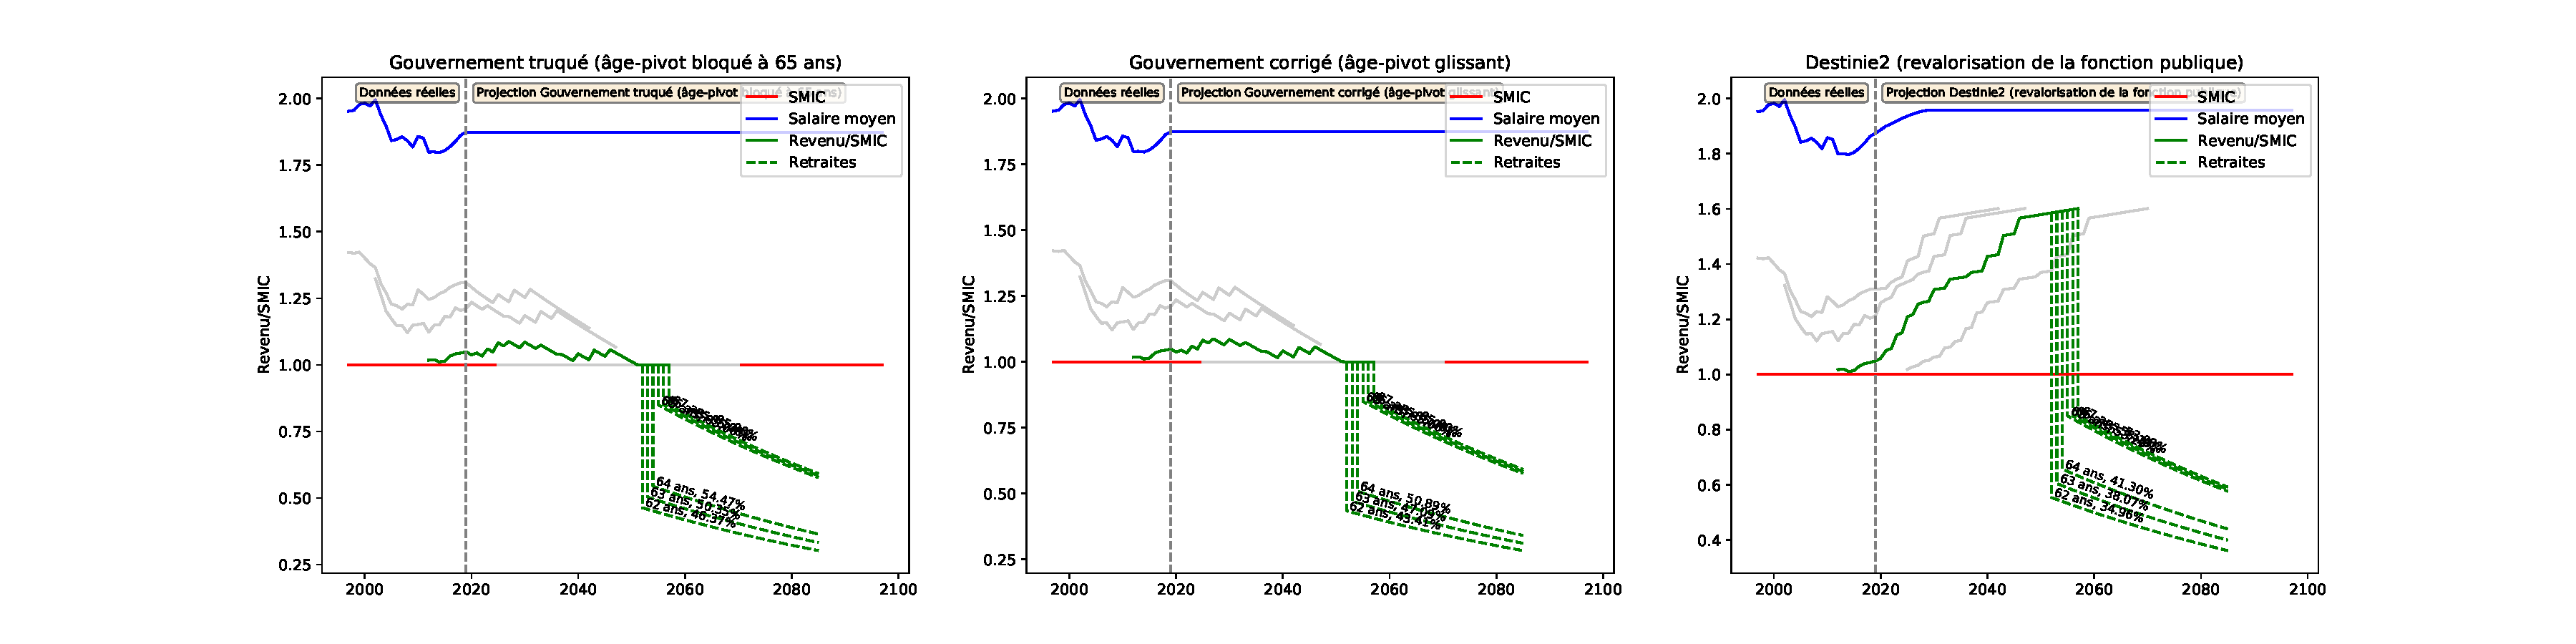
\includegraphics[width=0.9\textwidth]{fig/ATSEM_1990_22_dest_retraite.pdf}\end{center} \label{fig/ATSEM_1990_22_dest_retraite.pdf} 

\newpage 
 
\subsection{Génération 2003 (début en 2025)} 

\paragraph{Retraites possibles et ratios Revenu/SMIC à 70, 75, 80, 85, 90 ans avec le modèle \emph{Gouvernement truqué (âge-pivot bloqué à 65 ans)}}  
 
{ \scriptsize \begin{center} 
\begin{tabular}[htb]{|c|c||c|c||c|c||c||c|c|c|c|c|c|} 
\hline 
 Retraite en &  Âge &  Âge pivot &  Décote/Surcote &  Retraite (\euro{} 2019) &  Tx Rempl(\%) &  SMIC (\euro{} 2019) &  Retraite/SMIC &  Rev70/SMIC &  Rev75/SMIC &  Rev80/SMIC &  Rev85/SMIC &  Rev90/SMIC \\ 
\hline \hline 
 2065 &  62 &  65 ans 0 mois &  -15.00\% &  1457.41 &  {\bf 47.37} &  3076.71 &  {\bf {\color{red} 0.47}} &  {\bf {\color{red} 0.43}} &  {\bf {\color{red} 0.40}} &  {\bf {\color{red} 0.38}} &  {\bf {\color{red} 0.35}} &  {\bf {\color{red} 0.33}} \\ 
\hline 
 2066 &  63 &  65 ans 0 mois &  -10.00\% &  1602.25 &  {\bf 51.41} &  3116.71 &  {\bf {\color{red} 0.51}} &  {\bf {\color{red} 0.47}} &  {\bf {\color{red} 0.44}} &  {\bf {\color{red} 0.41}} &  {\bf {\color{red} 0.39}} &  {\bf {\color{red} 0.36}} \\ 
\hline 
 2067 &  64 &  65 ans 0 mois &  -5.00\% &  1755.00 &  {\bf 55.59} &  3157.23 &  {\bf {\color{red} 0.56}} &  {\bf {\color{red} 0.51}} &  {\bf {\color{red} 0.48}} &  {\bf {\color{red} 0.45}} &  {\bf {\color{red} 0.42}} &  {\bf {\color{red} 0.40}} \\ 
\hline 
 2068 &  65 &  65 ans 0 mois &  0.00\% &  2718.53 &  {\bf 85.00} &  3198.27 &  {\bf {\color{red} 0.85}} &  {\bf {\color{red} 0.80}} &  {\bf {\color{red} 0.75}} &  {\bf {\color{red} 0.70}} &  {\bf {\color{red} 0.66}} &  {\bf {\color{red} 0.62}} \\ 
\hline 
 2069 &  66 &  65 ans 0 mois &  5.00\% &  2753.87 &  {\bf 85.00} &  3239.85 &  {\bf {\color{red} 0.85}} &  {\bf {\color{red} 0.81}} &  {\bf {\color{red} 0.76}} &  {\bf {\color{red} 0.71}} &  {\bf {\color{red} 0.67}} &  {\bf {\color{red} 0.62}} \\ 
\hline 
 2070 &  67 &  65 ans 0 mois &  10.00\% &  2789.67 &  {\bf 85.00} &  3281.97 &  {\bf {\color{red} 0.85}} &  {\bf {\color{red} 0.82}} &  {\bf {\color{red} 0.77}} &  {\bf {\color{red} 0.72}} &  {\bf {\color{red} 0.67}} &  {\bf {\color{red} 0.63}} \\ 
\hline 
\hline 
\end{tabular} 
\end{center} } 
\paragraph{Retraites possibles et ratios Revenu/SMIC à 70, 75, 80, 85, 90 ans avec le modèle \emph{Gouvernement corrigé (âge-pivot glissant)}}  
 
{ \scriptsize \begin{center} 
\begin{tabular}[htb]{|c|c||c|c||c|c||c||c|c|c|c|c|c|} 
\hline 
 Retraite en &  Âge &  Âge pivot &  Décote/Surcote &  Retraite (\euro{} 2019) &  Tx Rempl(\%) &  SMIC (\euro{} 2019) &  Retraite/SMIC &  Rev70/SMIC &  Rev75/SMIC &  Rev80/SMIC &  Rev85/SMIC &  Rev90/SMIC \\ 
\hline \hline 
 2065 &  62 &  67 ans 2 mois &  -25.83\% &  1271.67 &  {\bf 41.33} &  3076.71 &  {\bf {\color{red} 0.41}} &  {\bf {\color{red} 0.37}} &  {\bf {\color{red} 0.35}} &  {\bf {\color{red} 0.33}} &  {\bf {\color{red} 0.31}} &  {\bf {\color{red} 0.29}} \\ 
\hline 
 2066 &  63 &  67 ans 3 mois &  -21.25\% &  1401.97 &  {\bf 44.98} &  3116.71 &  {\bf {\color{red} 0.45}} &  {\bf {\color{red} 0.41}} &  {\bf {\color{red} 0.39}} &  {\bf {\color{red} 0.36}} &  {\bf {\color{red} 0.34}} &  {\bf {\color{red} 0.32}} \\ 
\hline 
 2067 &  64 &  67 ans 4 mois &  -16.67\% &  1539.47 &  {\bf 48.76} &  3157.23 &  {\bf {\color{red} 0.49}} &  {\bf {\color{red} 0.45}} &  {\bf {\color{red} 0.42}} &  {\bf {\color{red} 0.40}} &  {\bf {\color{red} 0.37}} &  {\bf {\color{red} 0.35}} \\ 
\hline 
 2068 &  65 &  67 ans 5 mois &  -12.08\% &  2718.53 &  {\bf 85.00} &  3198.27 &  {\bf {\color{red} 0.85}} &  {\bf {\color{red} 0.80}} &  {\bf {\color{red} 0.75}} &  {\bf {\color{red} 0.70}} &  {\bf {\color{red} 0.66}} &  {\bf {\color{red} 0.62}} \\ 
\hline 
 2069 &  66 &  67 ans 6 mois &  -7.50\% &  2753.87 &  {\bf 85.00} &  3239.85 &  {\bf {\color{red} 0.85}} &  {\bf {\color{red} 0.81}} &  {\bf {\color{red} 0.76}} &  {\bf {\color{red} 0.71}} &  {\bf {\color{red} 0.67}} &  {\bf {\color{red} 0.62}} \\ 
\hline 
 2070 &  67 &  67 ans 7 mois &  -2.92\% &  2789.67 &  {\bf 85.00} &  3281.97 &  {\bf {\color{red} 0.85}} &  {\bf {\color{red} 0.82}} &  {\bf {\color{red} 0.77}} &  {\bf {\color{red} 0.72}} &  {\bf {\color{red} 0.67}} &  {\bf {\color{red} 0.63}} \\ 
\hline 
\hline 
\end{tabular} 
\end{center} } 
\paragraph{Retraites possibles et ratios Revenu/SMIC à 70, 75, 80, 85, 90 ans avec le modèle \emph{Destinie2 (revalorisation de la fonction publique)}}  
 
{ \scriptsize \begin{center} 
\begin{tabular}[htb]{|c|c||c|c||c|c||c||c|c|c|c|c|c|} 
\hline 
 Retraite en &  Âge &  Âge pivot &  Décote/Surcote &  Retraite (\euro{} 2019) &  Tx Rempl(\%) &  SMIC (\euro{} 2019) &  Retraite/SMIC &  Rev70/SMIC &  Rev75/SMIC &  Rev80/SMIC &  Rev85/SMIC &  Rev90/SMIC \\ 
\hline \hline 
 2065 &  62 &  67 ans 2 mois &  -25.83\% &  1640.50 &  {\bf 35.56} &  2892.68 &  {\bf {\color{red} 0.57}} &  {\bf {\color{red} 0.51}} &  {\bf {\color{red} 0.48}} &  {\bf {\color{red} 0.45}} &  {\bf {\color{red} 0.42}} &  {\bf {\color{red} 0.40}} \\ 
\hline 
 2066 &  63 &  67 ans 3 mois &  -21.25\% &  1815.76 &  {\bf 38.85} &  2930.29 &  {\bf {\color{red} 0.62}} &  {\bf {\color{red} 0.57}} &  {\bf {\color{red} 0.53}} &  {\bf {\color{red} 0.50}} &  {\bf {\color{red} 0.47}} &  {\bf {\color{red} 0.44}} \\ 
\hline 
 2067 &  64 &  67 ans 4 mois &  -16.67\% &  2001.34 &  {\bf 42.27} &  2968.38 &  {\bf {\color{red} 0.67}} &  {\bf {\color{red} 0.62}} &  {\bf {\color{red} 0.58}} &  {\bf {\color{red} 0.55}} &  {\bf {\color{red} 0.51}} &  {\bf {\color{red} 0.48}} \\ 
\hline 
 2068 &  65 &  67 ans 5 mois &  -12.08\% &  2555.93 &  {\bf 53.29} &  3006.97 &  {\bf {\color{red} 0.85}} &  {\bf {\color{red} 0.80}} &  {\bf {\color{red} 0.75}} &  {\bf {\color{red} 0.70}} &  {\bf {\color{red} 0.66}} &  {\bf {\color{red} 0.62}} \\ 
\hline 
 2069 &  66 &  67 ans 6 mois &  -7.50\% &  2589.15 &  {\bf 53.29} &  3046.06 &  {\bf {\color{red} 0.85}} &  {\bf {\color{red} 0.81}} &  {\bf {\color{red} 0.76}} &  {\bf {\color{red} 0.71}} &  {\bf {\color{red} 0.67}} &  {\bf {\color{red} 0.62}} \\ 
\hline 
 2070 &  67 &  67 ans 7 mois &  -2.92\% &  2623.20 &  {\bf 53.30} &  3085.66 &  {\bf {\color{red} 0.85}} &  {\bf {\color{red} 0.82}} &  {\bf {\color{red} 0.77}} &  {\bf {\color{red} 0.72}} &  {\bf {\color{red} 0.67}} &  {\bf {\color{red} 0.63}} \\ 
\hline 
\hline 
\end{tabular} 
\end{center} } 

 \begin{center}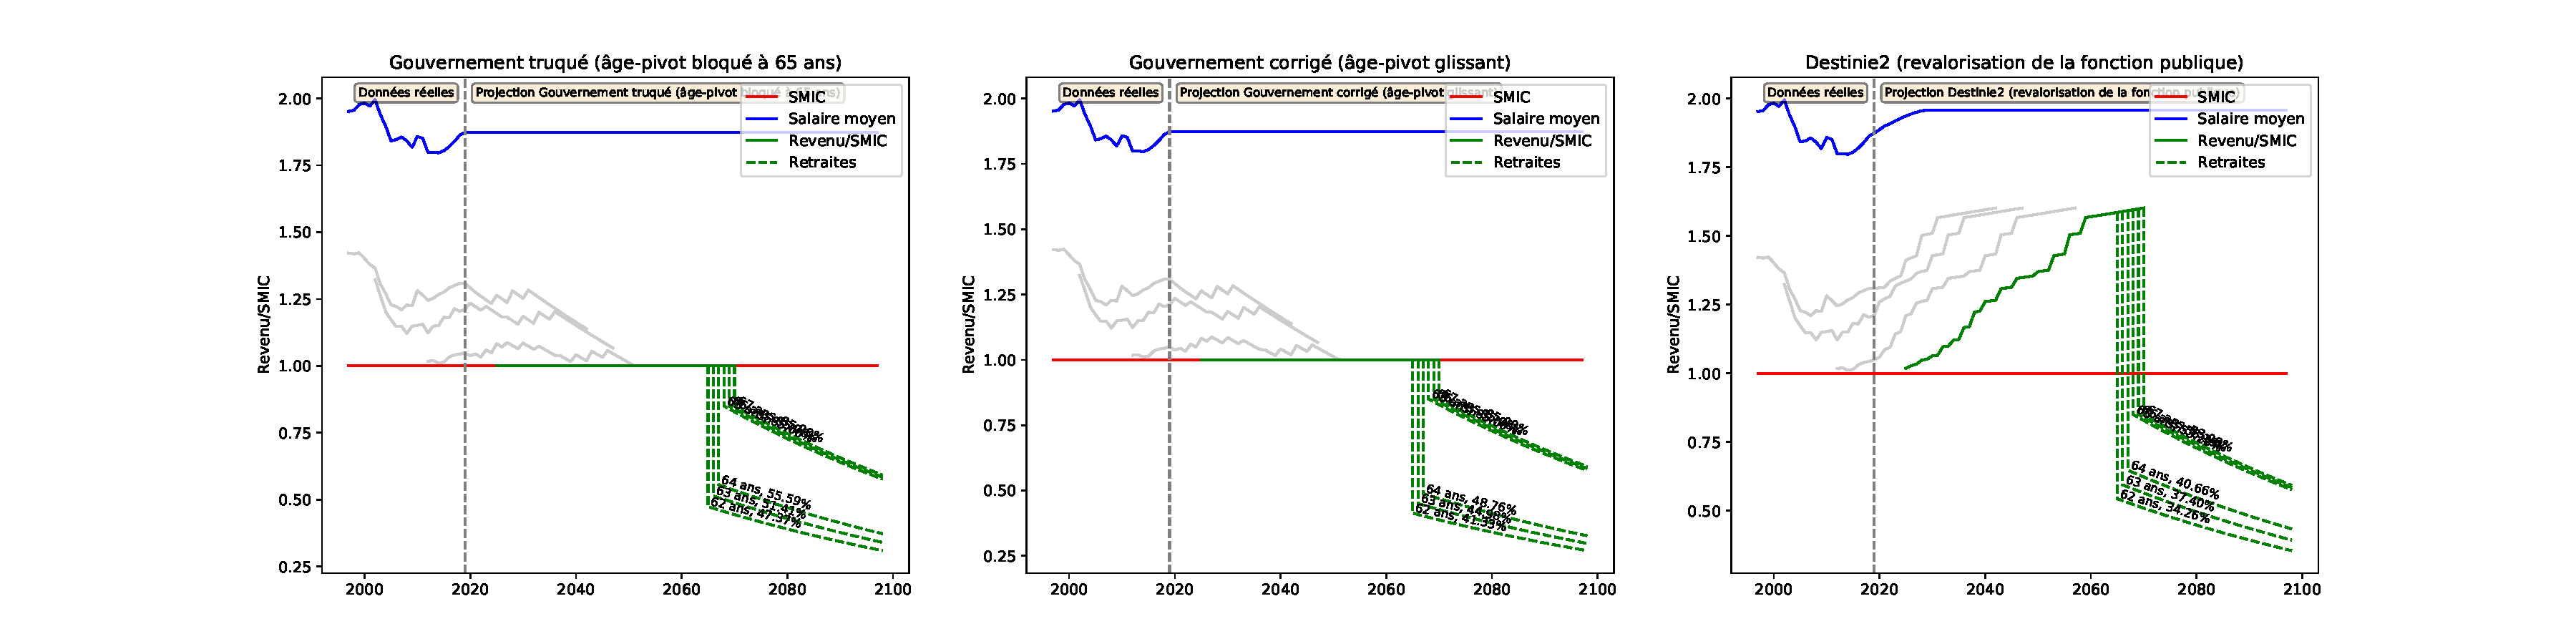
\includegraphics[width=0.9\textwidth]{fig/ATSEM_2003_22_dest_retraite.pdf}\end{center} \label{fig/ATSEM_2003_22_dest_retraite.pdf} 

\newpage 
 
\chapter{Professeur des écoles} 

\begin{minipage}{0.55\linewidth}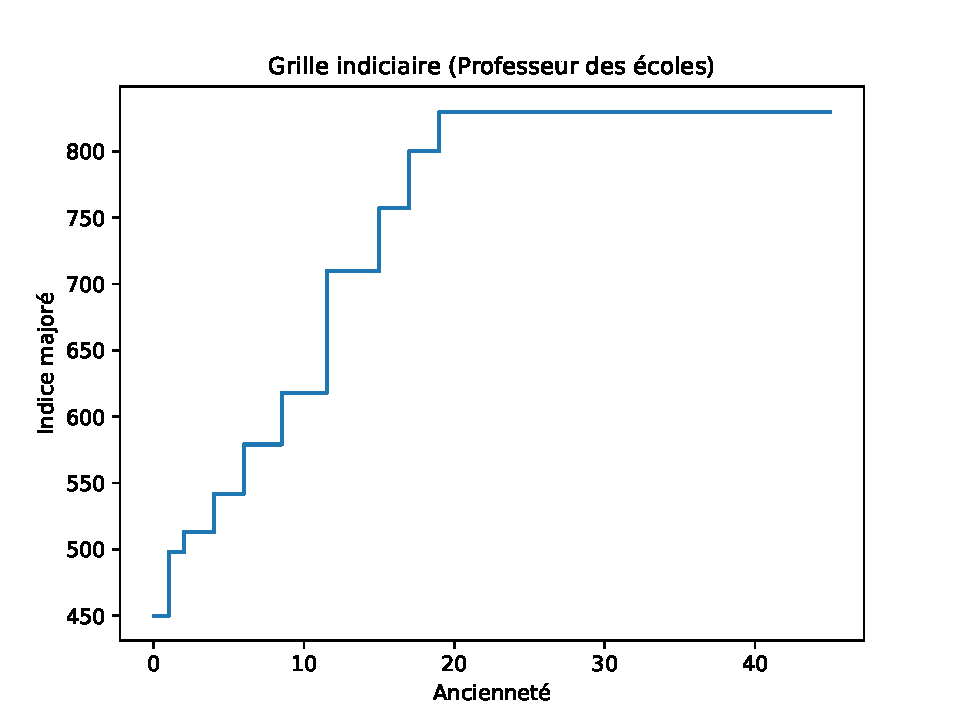
\includegraphics[width=0.7\textwidth]{fig/grille_ProfEcoles.pdf}\end{minipage} 
\begin{minipage}{0.3\linewidth} 
 \begin{center} 

\begin{tabular}[htb]{|c|c|} 
\hline 
 Indice majoré &  Durée (années) \\ 
\hline \hline 
 450 &  1.00 \\ 
\hline 
 498 &  1.00 \\ 
\hline 
 513 &  2.00 \\ 
\hline 
 542 &  2.00 \\ 
\hline 
 579 &  2.50 \\ 
\hline 
 618 &  3.00 \\ 
\hline 
 710 &  3.50 \\ 
\hline 
 757 &  2.00 \\ 
\hline 
 800 &  2.00 \\ 
\hline 
 830 &   \\ 
\hline 
\hline 
\end{tabular} 
\end{center} 
 \end{minipage} 


 \addto{\captionsenglish}{ \renewcommand{\mtctitle}{}} \setcounter{minitocdepth}{2} 
 \minitoc \newpage 

\section{Début de carrière à 22 ans} 

\subsection{Génération 1975 (début en 1997)} 

\paragraph{Retraites possibles et ratios Revenu/SMIC à 70, 75, 80, 85, 90 ans avec le modèle \emph{Gouvernement truqué (âge-pivot bloqué à 65 ans)}}  
 
{ \scriptsize \begin{center} 
\begin{tabular}[htb]{|c|c||c|c||c|c||c||c|c|c|c|c|c|} 
\hline 
 Retraite en &  Âge &  Âge pivot &  Décote/Surcote &  Retraite (\euro{} 2019) &  Tx Rempl(\%) &  SMIC (\euro{} 2019) &  Retraite/SMIC &  Rev70/SMIC &  Rev75/SMIC &  Rev80/SMIC &  Rev85/SMIC &  Rev90/SMIC \\ 
\hline \hline 
 2037 &  62 &  64 ans 10 mois &  -14.17\% &  1902.09 &  {\bf 44.50} &  2143.00 &  {\bf {\color{red} 0.89}} &  {\bf {\color{red} 0.80}} &  {\bf {\color{red} 0.75}} &  {\bf {\color{red} 0.70}} &  {\bf {\color{red} 0.66}} &  {\bf {\color{red} 0.62}} \\ 
\hline 
 2038 &  63 &  64 ans 11 mois &  -9.58\% &  2072.84 &  {\bf 48.39} &  2170.86 &  {\bf {\color{red} 0.95}} &  {\bf {\color{red} 0.87}} &  {\bf {\color{red} 0.82}} &  {\bf {\color{red} 0.77}} &  {\bf {\color{red} 0.72}} &  {\bf {\color{red} 0.67}} \\ 
\hline 
 2039 &  64 &  65 ans 0 mois &  -5.00\% &  2252.96 &  {\bf 52.49} &  2199.08 &  {\bf 1.02} &  {\bf {\color{red} 0.95}} &  {\bf {\color{red} 0.89}} &  {\bf {\color{red} 0.83}} &  {\bf {\color{red} 0.78}} &  {\bf {\color{red} 0.73}} \\ 
\hline 
 2040 &  65 &  65 ans 0 mois &  0.00\% &  2453.13 &  {\bf 57.03} &  2227.67 &  {\bf 1.10} &  {\bf 1.03} &  {\bf {\color{red} 0.97}} &  {\bf {\color{red} 0.91}} &  {\bf {\color{red} 0.85}} &  {\bf {\color{red} 0.80}} \\ 
\hline 
 2041 &  66 &  65 ans 0 mois &  5.00\% &  2664.36 &  {\bf 61.81} &  2256.63 &  {\bf 1.18} &  {\bf 1.12} &  {\bf 1.05} &  {\bf {\color{red} 0.99}} &  {\bf {\color{red} 0.92}} &  {\bf {\color{red} 0.87}} \\ 
\hline 
 2042 &  67 &  65 ans 0 mois &  10.00\% &  2887.23 &  {\bf 66.83} &  2285.97 &  {\bf 1.26} &  {\bf 1.22} &  {\bf 1.14} &  {\bf 1.07} &  {\bf 1.00} &  {\bf {\color{red} 0.94}} \\ 
\hline 
\hline 
\end{tabular} 
\end{center} } 
\paragraph{Retraites possibles et ratios Revenu/SMIC à 70, 75, 80, 85, 90 ans avec le modèle \emph{Gouvernement corrigé (âge-pivot glissant)}}  
 
{ \scriptsize \begin{center} 
\begin{tabular}[htb]{|c|c||c|c||c|c||c||c|c|c|c|c|c|} 
\hline 
 Retraite en &  Âge &  Âge pivot &  Décote/Surcote &  Retraite (\euro{} 2019) &  Tx Rempl(\%) &  SMIC (\euro{} 2019) &  Retraite/SMIC &  Rev70/SMIC &  Rev75/SMIC &  Rev80/SMIC &  Rev85/SMIC &  Rev90/SMIC \\ 
\hline \hline 
 2037 &  62 &  64 ans 10 mois &  -14.17\% &  1902.09 &  {\bf 44.50} &  2143.00 &  {\bf {\color{red} 0.89}} &  {\bf {\color{red} 0.80}} &  {\bf {\color{red} 0.75}} &  {\bf {\color{red} 0.70}} &  {\bf {\color{red} 0.66}} &  {\bf {\color{red} 0.62}} \\ 
\hline 
 2038 &  63 &  64 ans 11 mois &  -9.58\% &  2072.84 &  {\bf 48.39} &  2170.86 &  {\bf {\color{red} 0.95}} &  {\bf {\color{red} 0.87}} &  {\bf {\color{red} 0.82}} &  {\bf {\color{red} 0.77}} &  {\bf {\color{red} 0.72}} &  {\bf {\color{red} 0.67}} \\ 
\hline 
 2039 &  64 &  65 ans 0 mois &  -5.00\% &  2252.96 &  {\bf 52.49} &  2199.08 &  {\bf 1.02} &  {\bf {\color{red} 0.95}} &  {\bf {\color{red} 0.89}} &  {\bf {\color{red} 0.83}} &  {\bf {\color{red} 0.78}} &  {\bf {\color{red} 0.73}} \\ 
\hline 
 2040 &  65 &  65 ans 1 mois &  -0.42\% &  2442.91 &  {\bf 56.79} &  2227.67 &  {\bf 1.10} &  {\bf 1.03} &  {\bf {\color{red} 0.96}} &  {\bf {\color{red} 0.90}} &  {\bf {\color{red} 0.85}} &  {\bf {\color{red} 0.79}} \\ 
\hline 
 2041 &  66 &  65 ans 2 mois &  4.17\% &  2643.22 &  {\bf 61.32} &  2256.63 &  {\bf 1.17} &  {\bf 1.11} &  {\bf 1.04} &  {\bf {\color{red} 0.98}} &  {\bf {\color{red} 0.92}} &  {\bf {\color{red} 0.86}} \\ 
\hline 
 2042 &  67 &  65 ans 3 mois &  8.75\% &  2854.42 &  {\bf 66.07} &  2285.97 &  {\bf 1.25} &  {\bf 1.20} &  {\bf 1.13} &  {\bf 1.06} &  {\bf {\color{red} 0.99}} &  {\bf {\color{red} 0.93}} \\ 
\hline 
\hline 
\end{tabular} 
\end{center} } 
\paragraph{Retraites possibles et ratios Revenu/SMIC à 70, 75, 80, 85, 90 ans avec le modèle \emph{Destinie2 (revalorisation de la fonction publique)}}  
 
{ \scriptsize \begin{center} 
\begin{tabular}[htb]{|c|c||c|c||c|c||c||c|c|c|c|c|c|} 
\hline 
 Retraite en &  Âge &  Âge pivot &  Décote/Surcote &  Retraite (\euro{} 2019) &  Tx Rempl(\%) &  SMIC (\euro{} 2019) &  Retraite/SMIC &  Rev70/SMIC &  Rev75/SMIC &  Rev80/SMIC &  Rev85/SMIC &  Rev90/SMIC \\ 
\hline \hline 
 2037 &  62 &  64 ans 10 mois &  -14.17\% &  2101.92 &  {\bf 39.41} &  2014.82 &  {\bf 1.04} &  {\bf {\color{red} 0.94}} &  {\bf {\color{red} 0.88}} &  {\bf {\color{red} 0.83}} &  {\bf {\color{red} 0.78}} &  {\bf {\color{red} 0.73}} \\ 
\hline 
 2038 &  63 &  64 ans 11 mois &  -9.58\% &  2299.05 &  {\bf 42.55} &  2041.01 &  {\bf 1.13} &  {\bf 1.03} &  {\bf {\color{red} 0.96}} &  {\bf {\color{red} 0.90}} &  {\bf {\color{red} 0.85}} &  {\bf {\color{red} 0.79}} \\ 
\hline 
 2039 &  64 &  65 ans 0 mois &  -5.00\% &  2508.24 &  {\bf 45.82} &  2067.55 &  {\bf 1.21} &  {\bf 1.12} &  {\bf 1.05} &  {\bf {\color{red} 0.99}} &  {\bf {\color{red} 0.92}} &  {\bf {\color{red} 0.87}} \\ 
\hline 
 2040 &  65 &  65 ans 1 mois &  -0.42\% &  2730.19 &  {\bf 49.24} &  2094.43 &  {\bf 1.30} &  {\bf 1.22} &  {\bf 1.15} &  {\bf 1.07} &  {\bf 1.01} &  {\bf {\color{red} 0.94}} \\ 
\hline 
 2041 &  66 &  65 ans 2 mois &  4.17\% &  2965.64 &  {\bf 52.80} &  2121.65 &  {\bf 1.40} &  {\bf 1.33} &  {\bf 1.24} &  {\bf 1.17} &  {\bf 1.09} &  {\bf 1.03} \\ 
\hline 
 2042 &  67 &  65 ans 3 mois &  8.75\% &  3215.36 &  {\bf 56.51} &  2149.23 &  {\bf 1.50} &  {\bf 1.44} &  {\bf 1.35} &  {\bf 1.26} &  {\bf 1.19} &  {\bf 1.11} \\ 
\hline 
\hline 
\end{tabular} 
\end{center} } 

 \begin{center}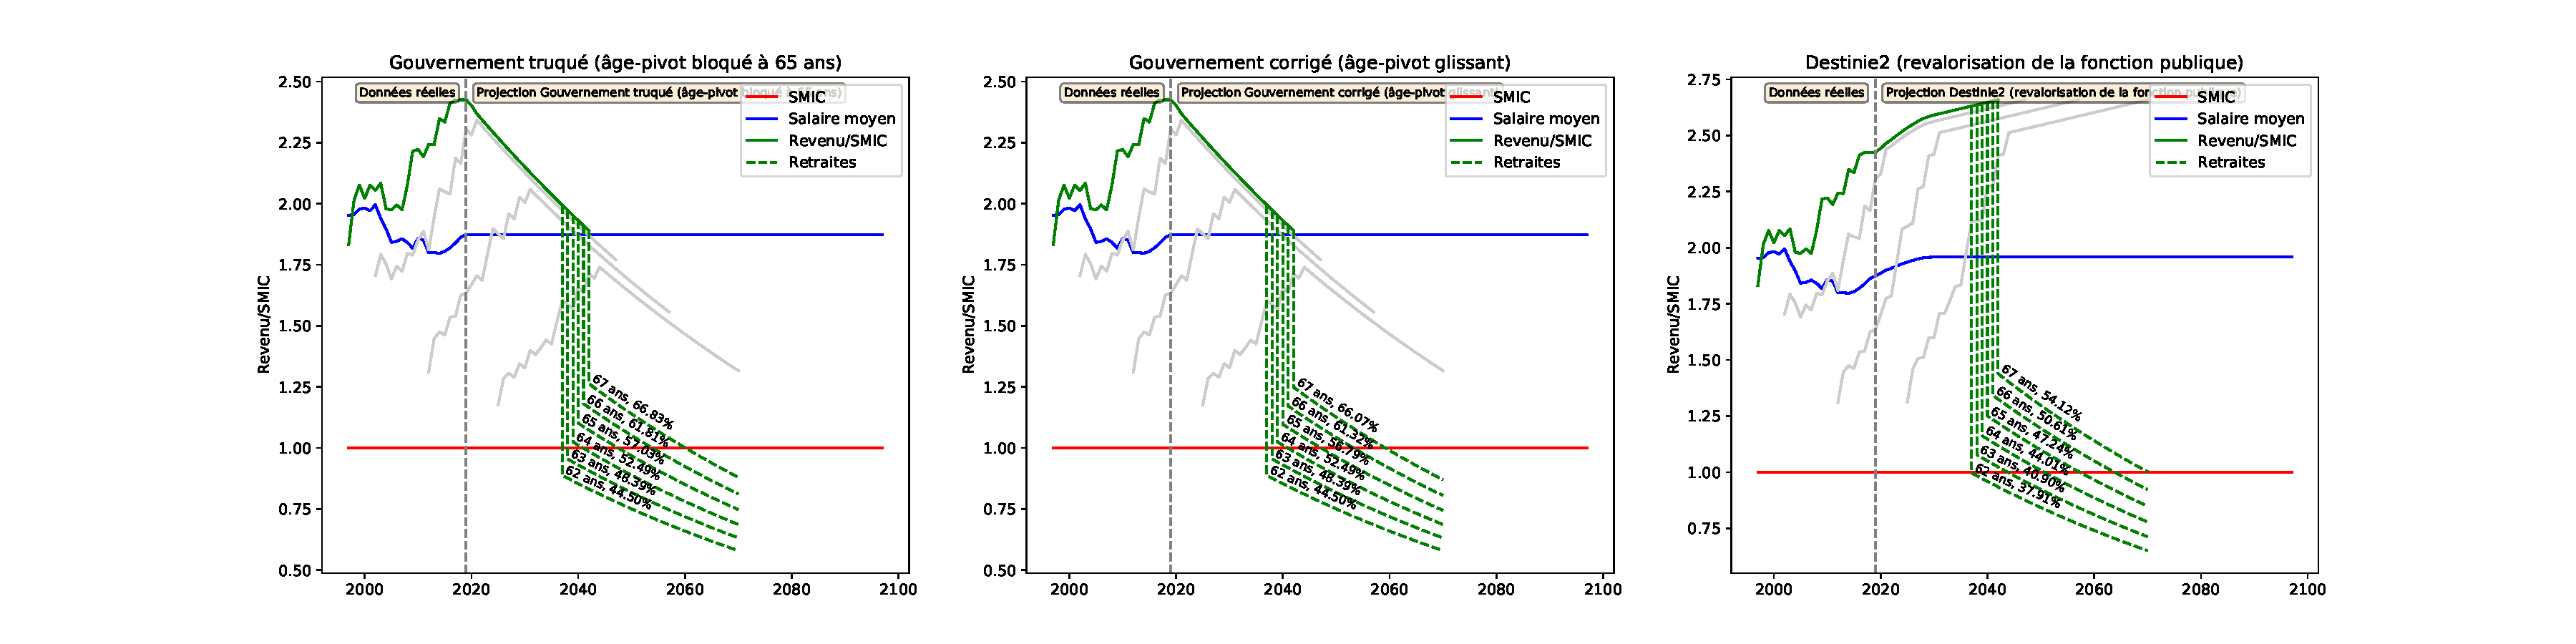
\includegraphics[width=0.9\textwidth]{fig/ProfEcoles_1975_22_dest_retraite.pdf}\end{center} \label{fig/ProfEcoles_1975_22_dest_retraite.pdf} 

\newpage 
 
\subsection{Génération 1980 (début en 2002)} 

\paragraph{Retraites possibles et ratios Revenu/SMIC à 70, 75, 80, 85, 90 ans avec le modèle \emph{Gouvernement truqué (âge-pivot bloqué à 65 ans)}}  
 
{ \scriptsize \begin{center} 
\begin{tabular}[htb]{|c|c||c|c||c|c||c||c|c|c|c|c|c|} 
\hline 
 Retraite en &  Âge &  Âge pivot &  Décote/Surcote &  Retraite (\euro{} 2019) &  Tx Rempl(\%) &  SMIC (\euro{} 2019) &  Retraite/SMIC &  Rev70/SMIC &  Rev75/SMIC &  Rev80/SMIC &  Rev85/SMIC &  Rev90/SMIC \\ 
\hline \hline 
 2042 &  62 &  65 ans 0 mois &  -15.00\% &  1925.24 &  {\bf 45.04} &  2285.97 &  {\bf {\color{red} 0.84}} &  {\bf {\color{red} 0.76}} &  {\bf {\color{red} 0.71}} &  {\bf {\color{red} 0.67}} &  {\bf {\color{red} 0.63}} &  {\bf {\color{red} 0.59}} \\ 
\hline 
 2043 &  63 &  65 ans 0 mois &  -10.00\% &  2115.51 &  {\bf 49.39} &  2315.68 &  {\bf {\color{red} 0.91}} &  {\bf {\color{red} 0.83}} &  {\bf {\color{red} 0.78}} &  {\bf {\color{red} 0.73}} &  {\bf {\color{red} 0.69}} &  {\bf {\color{red} 0.64}} \\ 
\hline 
 2044 &  64 &  65 ans 0 mois &  -5.00\% &  2317.12 &  {\bf 53.98} &  2345.79 &  {\bf {\color{red} 0.99}} &  {\bf {\color{red} 0.91}} &  {\bf {\color{red} 0.86}} &  {\bf {\color{red} 0.80}} &  {\bf {\color{red} 0.75}} &  {\bf {\color{red} 0.71}} \\ 
\hline 
 2045 &  65 &  65 ans 0 mois &  0.00\% &  2530.65 &  {\bf 58.83} &  2376.28 &  {\bf 1.06} &  {\bf {\color{red} 1.00}} &  {\bf {\color{red} 0.94}} &  {\bf {\color{red} 0.88}} &  {\bf {\color{red} 0.82}} &  {\bf {\color{red} 0.77}} \\ 
\hline 
 2046 &  66 &  65 ans 0 mois &  5.00\% &  2754.73 &  {\bf 63.90} &  2407.18 &  {\bf 1.14} &  {\bf 1.09} &  {\bf 1.02} &  {\bf {\color{red} 0.96}} &  {\bf {\color{red} 0.90}} &  {\bf {\color{red} 0.84}} \\ 
\hline 
 2047 &  67 &  65 ans 0 mois &  10.00\% &  2989.57 &  {\bf 69.20} &  2438.47 &  {\bf 1.23} &  {\bf 1.18} &  {\bf 1.11} &  {\bf 1.04} &  {\bf {\color{red} 0.97}} &  {\bf {\color{red} 0.91}} \\ 
\hline 
\hline 
\end{tabular} 
\end{center} } 
\paragraph{Retraites possibles et ratios Revenu/SMIC à 70, 75, 80, 85, 90 ans avec le modèle \emph{Gouvernement corrigé (âge-pivot glissant)}}  
 
{ \scriptsize \begin{center} 
\begin{tabular}[htb]{|c|c||c|c||c|c||c||c|c|c|c|c|c|} 
\hline 
 Retraite en &  Âge &  Âge pivot &  Décote/Surcote &  Retraite (\euro{} 2019) &  Tx Rempl(\%) &  SMIC (\euro{} 2019) &  Retraite/SMIC &  Rev70/SMIC &  Rev75/SMIC &  Rev80/SMIC &  Rev85/SMIC &  Rev90/SMIC \\ 
\hline \hline 
 2042 &  62 &  65 ans 3 mois &  -16.25\% &  1896.93 &  {\bf 44.38} &  2285.97 &  {\bf {\color{red} 0.83}} &  {\bf {\color{red} 0.75}} &  {\bf {\color{red} 0.70}} &  {\bf {\color{red} 0.66}} &  {\bf {\color{red} 0.62}} &  {\bf {\color{red} 0.58}} \\ 
\hline 
 2043 &  63 &  65 ans 4 mois &  -11.67\% &  2076.34 &  {\bf 48.47} &  2315.68 &  {\bf {\color{red} 0.90}} &  {\bf {\color{red} 0.82}} &  {\bf {\color{red} 0.77}} &  {\bf {\color{red} 0.72}} &  {\bf {\color{red} 0.67}} &  {\bf {\color{red} 0.63}} \\ 
\hline 
 2044 &  64 &  65 ans 5 mois &  -7.08\% &  2266.30 &  {\bf 52.80} &  2345.79 &  {\bf {\color{red} 0.97}} &  {\bf {\color{red} 0.89}} &  {\bf {\color{red} 0.84}} &  {\bf {\color{red} 0.79}} &  {\bf {\color{red} 0.74}} &  {\bf {\color{red} 0.69}} \\ 
\hline 
 2045 &  65 &  65 ans 6 mois &  -2.50\% &  2467.39 &  {\bf 57.36} &  2376.28 &  {\bf 1.04} &  {\bf {\color{red} 0.97}} &  {\bf {\color{red} 0.91}} &  {\bf {\color{red} 0.86}} &  {\bf {\color{red} 0.80}} &  {\bf {\color{red} 0.75}} \\ 
\hline 
 2046 &  66 &  65 ans 7 mois &  2.08\% &  2678.21 &  {\bf 62.13} &  2407.18 &  {\bf 1.11} &  {\bf 1.06} &  {\bf {\color{red} 0.99}} &  {\bf {\color{red} 0.93}} &  {\bf {\color{red} 0.87}} &  {\bf {\color{red} 0.82}} \\ 
\hline 
 2047 &  67 &  65 ans 8 mois &  6.67\% &  2898.98 &  {\bf 67.11} &  2438.47 &  {\bf 1.19} &  {\bf 1.14} &  {\bf 1.07} &  {\bf 1.01} &  {\bf {\color{red} 0.94}} &  {\bf {\color{red} 0.88}} \\ 
\hline 
\hline 
\end{tabular} 
\end{center} } 
\paragraph{Retraites possibles et ratios Revenu/SMIC à 70, 75, 80, 85, 90 ans avec le modèle \emph{Destinie2 (revalorisation de la fonction publique)}}  
 
{ \scriptsize \begin{center} 
\begin{tabular}[htb]{|c|c||c|c||c|c||c||c|c|c|c|c|c|} 
\hline 
 Retraite en &  Âge &  Âge pivot &  Décote/Surcote &  Retraite (\euro{} 2019) &  Tx Rempl(\%) &  SMIC (\euro{} 2019) &  Retraite/SMIC &  Rev70/SMIC &  Rev75/SMIC &  Rev80/SMIC &  Rev85/SMIC &  Rev90/SMIC \\ 
\hline \hline 
 2042 &  62 &  65 ans 3 mois &  -16.25\% &  2171.58 &  {\bf 38.17} &  2149.23 &  {\bf 1.01} &  {\bf {\color{red} 0.91}} &  {\bf {\color{red} 0.85}} &  {\bf {\color{red} 0.80}} &  {\bf {\color{red} 0.75}} &  {\bf {\color{red} 0.70}} \\ 
\hline 
 2043 &  63 &  65 ans 4 mois &  -11.67\% &  2387.54 &  {\bf 41.42} &  2177.17 &  {\bf 1.10} &  {\bf 1.00} &  {\bf {\color{red} 0.94}} &  {\bf {\color{red} 0.88}} &  {\bf {\color{red} 0.83}} &  {\bf {\color{red} 0.77}} \\ 
\hline 
 2044 &  64 &  65 ans 5 mois &  -7.08\% &  2617.66 &  {\bf 44.83} &  2205.48 &  {\bf 1.19} &  {\bf 1.10} &  {\bf 1.03} &  {\bf {\color{red} 0.97}} &  {\bf {\color{red} 0.90}} &  {\bf {\color{red} 0.85}} \\ 
\hline 
 2045 &  65 &  65 ans 6 mois &  -2.50\% &  2862.76 &  {\bf 48.40} &  2234.15 &  {\bf 1.28} &  {\bf 1.20} &  {\bf 1.13} &  {\bf 1.06} &  {\bf {\color{red} 0.99}} &  {\bf {\color{red} 0.93}} \\ 
\hline 
 2046 &  66 &  65 ans 7 mois &  2.08\% &  3121.43 &  {\bf 52.10} &  2263.19 &  {\bf 1.38} &  {\bf 1.31} &  {\bf 1.23} &  {\bf 1.15} &  {\bf 1.08} &  {\bf 1.01} \\ 
\hline 
 2047 &  67 &  65 ans 8 mois &  6.67\% &  3394.09 &  {\bf 55.92} &  2292.61 &  {\bf 1.48} &  {\bf 1.42} &  {\bf 1.34} &  {\bf 1.25} &  {\bf 1.17} &  {\bf 1.10} \\ 
\hline 
\hline 
\end{tabular} 
\end{center} } 

 \begin{center}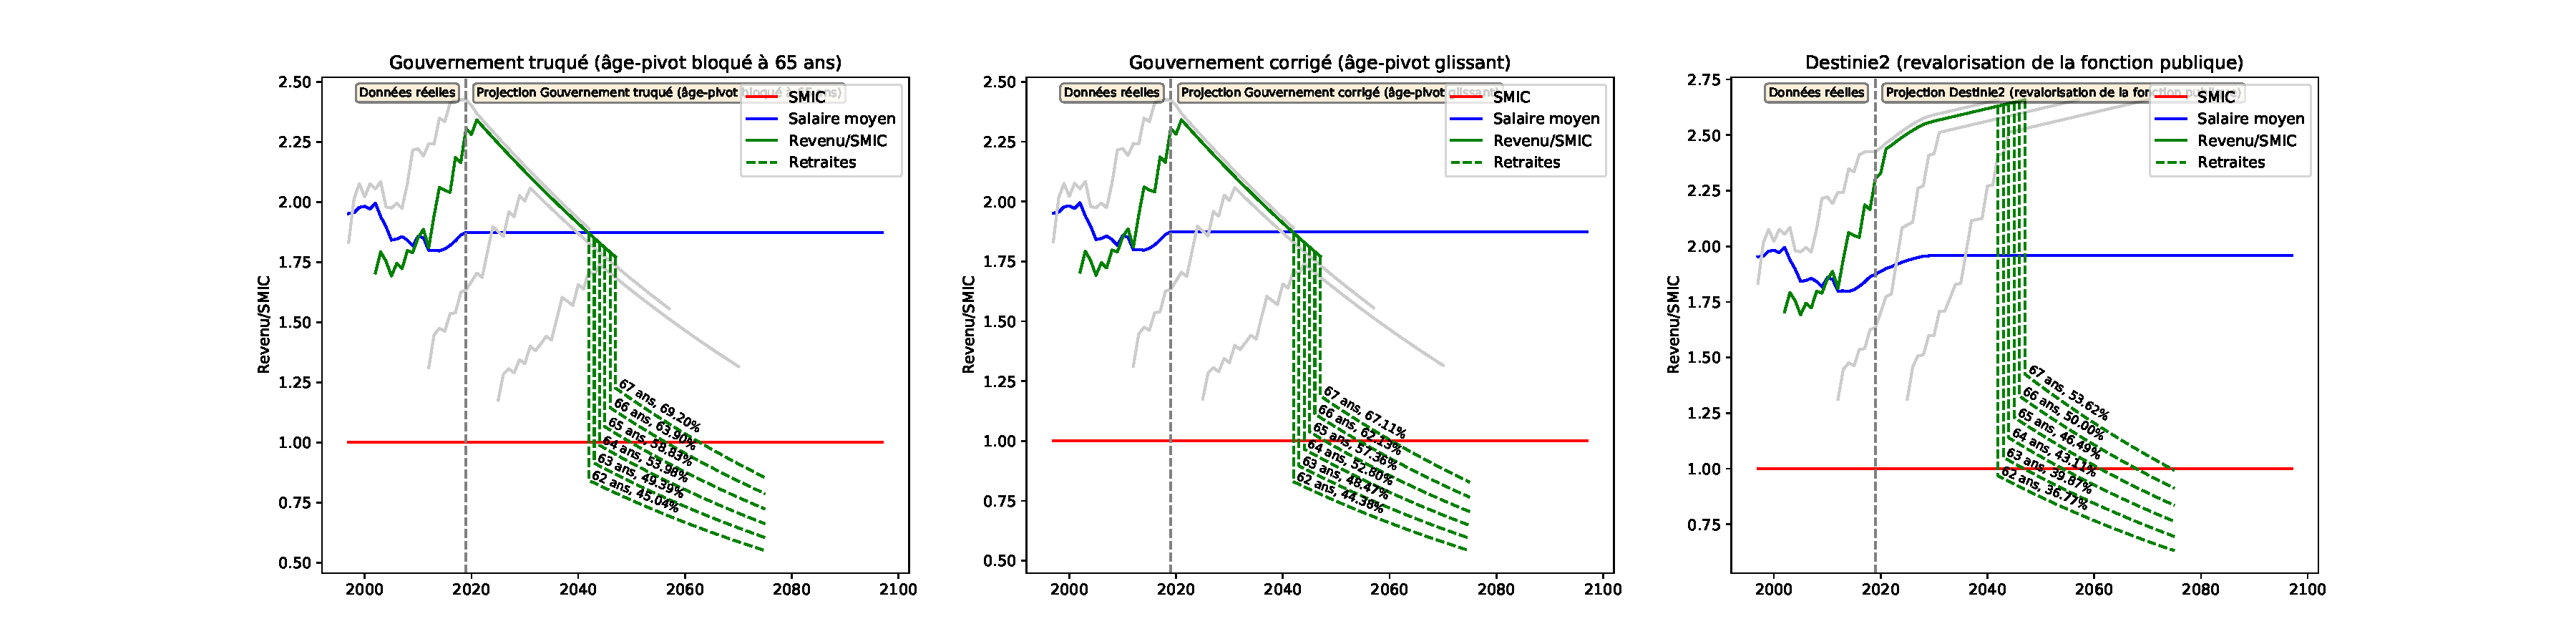
\includegraphics[width=0.9\textwidth]{fig/ProfEcoles_1980_22_dest_retraite.pdf}\end{center} \label{fig/ProfEcoles_1980_22_dest_retraite.pdf} 

\newpage 
 
\subsection{Génération 1990 (début en 2012)} 

\paragraph{Retraites possibles et ratios Revenu/SMIC à 70, 75, 80, 85, 90 ans avec le modèle \emph{Gouvernement truqué (âge-pivot bloqué à 65 ans)}}  
 
{ \scriptsize \begin{center} 
\begin{tabular}[htb]{|c|c||c|c||c|c||c||c|c|c|c|c|c|} 
\hline 
 Retraite en &  Âge &  Âge pivot &  Décote/Surcote &  Retraite (\euro{} 2019) &  Tx Rempl(\%) &  SMIC (\euro{} 2019) &  Retraite/SMIC &  Rev70/SMIC &  Rev75/SMIC &  Rev80/SMIC &  Rev85/SMIC &  Rev90/SMIC \\ 
\hline \hline 
 2052 &  62 &  65 ans 0 mois &  -15.00\% &  2069.04 &  {\bf 48.41} &  2601.14 &  {\bf {\color{red} 0.80}} &  {\bf {\color{red} 0.72}} &  {\bf {\color{red} 0.67}} &  {\bf {\color{red} 0.63}} &  {\bf {\color{red} 0.59}} &  {\bf {\color{red} 0.55}} \\ 
\hline 
 2053 &  63 &  65 ans 0 mois &  -10.00\% &  2272.88 &  {\bf 53.06} &  2634.96 &  {\bf {\color{red} 0.86}} &  {\bf {\color{red} 0.79}} &  {\bf {\color{red} 0.74}} &  {\bf {\color{red} 0.69}} &  {\bf {\color{red} 0.65}} &  {\bf {\color{red} 0.61}} \\ 
\hline 
 2054 &  64 &  65 ans 0 mois &  -5.00\% &  2487.11 &  {\bf 57.94} &  2669.21 &  {\bf {\color{red} 0.93}} &  {\bf {\color{red} 0.86}} &  {\bf {\color{red} 0.81}} &  {\bf {\color{red} 0.76}} &  {\bf {\color{red} 0.71}} &  {\bf {\color{red} 0.67}} \\ 
\hline 
 2055 &  65 &  65 ans 0 mois &  0.00\% &  2711.92 &  {\bf 63.04} &  2703.91 &  {\bf 1.00} &  {\bf {\color{red} 0.94}} &  {\bf {\color{red} 0.88}} &  {\bf {\color{red} 0.83}} &  {\bf {\color{red} 0.77}} &  {\bf {\color{red} 0.73}} \\ 
\hline 
 2056 &  66 &  65 ans 0 mois &  5.00\% &  2947.54 &  {\bf 68.37} &  2739.06 &  {\bf 1.08} &  {\bf 1.02} &  {\bf {\color{red} 0.96}} &  {\bf {\color{red} 0.90}} &  {\bf {\color{red} 0.84}} &  {\bf {\color{red} 0.79}} \\ 
\hline 
 2057 &  67 &  65 ans 0 mois &  10.00\% &  3194.18 &  {\bf 73.94} &  2774.67 &  {\bf 1.15} &  {\bf 1.11} &  {\bf 1.04} &  {\bf {\color{red} 0.97}} &  {\bf {\color{red} 0.91}} &  {\bf {\color{red} 0.86}} \\ 
\hline 
\hline 
\end{tabular} 
\end{center} } 
\paragraph{Retraites possibles et ratios Revenu/SMIC à 70, 75, 80, 85, 90 ans avec le modèle \emph{Gouvernement corrigé (âge-pivot glissant)}}  
 
{ \scriptsize \begin{center} 
\begin{tabular}[htb]{|c|c||c|c||c|c||c||c|c|c|c|c|c|} 
\hline 
 Retraite en &  Âge &  Âge pivot &  Décote/Surcote &  Retraite (\euro{} 2019) &  Tx Rempl(\%) &  SMIC (\euro{} 2019) &  Retraite/SMIC &  Rev70/SMIC &  Rev75/SMIC &  Rev80/SMIC &  Rev85/SMIC &  Rev90/SMIC \\ 
\hline \hline 
 2052 &  62 &  66 ans 1 mois &  -20.42\% &  1937.19 &  {\bf 45.32} &  2601.14 &  {\bf {\color{red} 0.74}} &  {\bf {\color{red} 0.67}} &  {\bf {\color{red} 0.63}} &  {\bf {\color{red} 0.59}} &  {\bf {\color{red} 0.55}} &  {\bf {\color{red} 0.52}} \\ 
\hline 
 2053 &  63 &  66 ans 2 mois &  -15.83\% &  2125.57 &  {\bf 49.62} &  2634.96 &  {\bf {\color{red} 0.81}} &  {\bf {\color{red} 0.74}} &  {\bf {\color{red} 0.69}} &  {\bf {\color{red} 0.65}} &  {\bf {\color{red} 0.61}} &  {\bf {\color{red} 0.57}} \\ 
\hline 
 2054 &  64 &  66 ans 3 mois &  -11.25\% &  2323.48 &  {\bf 54.13} &  2669.21 &  {\bf {\color{red} 0.87}} &  {\bf {\color{red} 0.81}} &  {\bf {\color{red} 0.76}} &  {\bf {\color{red} 0.71}} &  {\bf {\color{red} 0.66}} &  {\bf {\color{red} 0.62}} \\ 
\hline 
 2055 &  65 &  66 ans 4 mois &  -6.67\% &  2531.12 &  {\bf 58.84} &  2703.91 &  {\bf {\color{red} 0.94}} &  {\bf {\color{red} 0.88}} &  {\bf {\color{red} 0.82}} &  {\bf {\color{red} 0.77}} &  {\bf {\color{red} 0.72}} &  {\bf {\color{red} 0.68}} \\ 
\hline 
 2056 &  66 &  66 ans 5 mois &  -2.08\% &  2748.69 &  {\bf 63.76} &  2739.06 &  {\bf 1.00} &  {\bf {\color{red} 0.95}} &  {\bf {\color{red} 0.89}} &  {\bf {\color{red} 0.84}} &  {\bf {\color{red} 0.79}} &  {\bf {\color{red} 0.74}} \\ 
\hline 
 2057 &  67 &  66 ans 6 mois &  2.50\% &  2976.40 &  {\bf 68.90} &  2774.67 &  {\bf 1.07} &  {\bf 1.03} &  {\bf {\color{red} 0.97}} &  {\bf {\color{red} 0.91}} &  {\bf {\color{red} 0.85}} &  {\bf {\color{red} 0.80}} \\ 
\hline 
\hline 
\end{tabular} 
\end{center} } 
\paragraph{Retraites possibles et ratios Revenu/SMIC à 70, 75, 80, 85, 90 ans avec le modèle \emph{Destinie2 (revalorisation de la fonction publique)}}  
 
{ \scriptsize \begin{center} 
\begin{tabular}[htb]{|c|c||c|c||c|c||c||c|c|c|c|c|c|} 
\hline 
 Retraite en &  Âge &  Âge pivot &  Décote/Surcote &  Retraite (\euro{} 2019) &  Tx Rempl(\%) &  SMIC (\euro{} 2019) &  Retraite/SMIC &  Rev70/SMIC &  Rev75/SMIC &  Rev80/SMIC &  Rev85/SMIC &  Rev90/SMIC \\ 
\hline \hline 
 2052 &  62 &  66 ans 1 mois &  -20.42\% &  2436.82 &  {\bf 37.64} &  2445.56 &  {\bf {\color{red} 1.00}} &  {\bf {\color{red} 0.90}} &  {\bf {\color{red} 0.84}} &  {\bf {\color{red} 0.79}} &  {\bf {\color{red} 0.74}} &  {\bf {\color{red} 0.69}} \\ 
\hline 
 2053 &  63 &  66 ans 2 mois &  -15.83\% &  2687.50 &  {\bf 40.98} &  2477.35 &  {\bf 1.08} &  {\bf {\color{red} 0.99}} &  {\bf {\color{red} 0.93}} &  {\bf {\color{red} 0.87}} &  {\bf {\color{red} 0.82}} &  {\bf {\color{red} 0.77}} \\ 
\hline 
 2054 &  64 &  66 ans 3 mois &  -11.25\% &  2952.76 &  {\bf 44.44} &  2509.56 &  {\bf 1.18} &  {\bf 1.09} &  {\bf 1.02} &  {\bf {\color{red} 0.96}} &  {\bf {\color{red} 0.90}} &  {\bf {\color{red} 0.84}} \\ 
\hline 
 2055 &  65 &  66 ans 4 mois &  -6.67\% &  3233.05 &  {\bf 48.04} &  2542.18 &  {\bf 1.27} &  {\bf 1.19} &  {\bf 1.12} &  {\bf 1.05} &  {\bf {\color{red} 0.98}} &  {\bf {\color{red} 0.92}} \\ 
\hline 
 2056 &  66 &  66 ans 5 mois &  -2.08\% &  3528.83 &  {\bf 51.76} &  2575.23 &  {\bf 1.37} &  {\bf 1.30} &  {\bf 1.22} &  {\bf 1.14} &  {\bf 1.07} &  {\bf 1.01} \\ 
\hline 
 2057 &  67 &  66 ans 6 mois &  2.50\% &  3840.56 &  {\bf 55.61} &  2608.71 &  {\bf 1.47} &  {\bf 1.42} &  {\bf 1.33} &  {\bf 1.24} &  {\bf 1.17} &  {\bf 1.09} \\ 
\hline 
\hline 
\end{tabular} 
\end{center} } 

 \begin{center}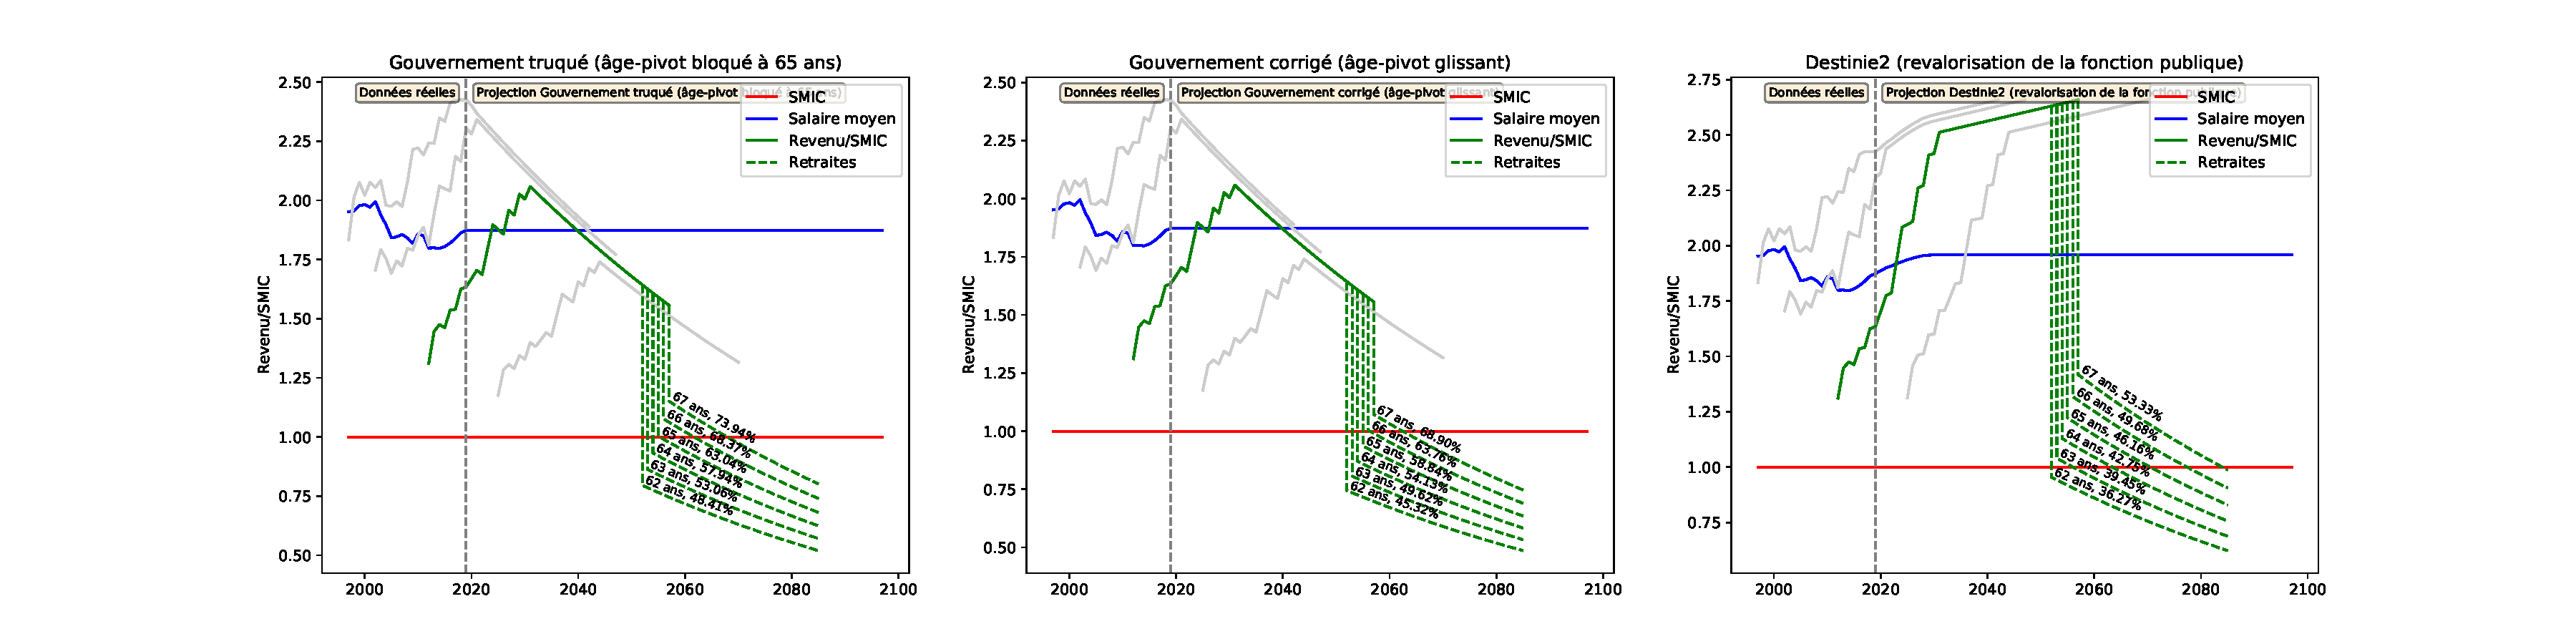
\includegraphics[width=0.9\textwidth]{fig/ProfEcoles_1990_22_dest_retraite.pdf}\end{center} \label{fig/ProfEcoles_1990_22_dest_retraite.pdf} 

\newpage 
 
\subsection{Génération 2003 (début en 2025)} 

\paragraph{Retraites possibles et ratios Revenu/SMIC à 70, 75, 80, 85, 90 ans avec le modèle \emph{Gouvernement truqué (âge-pivot bloqué à 65 ans)}}  
 
{ \scriptsize \begin{center} 
\begin{tabular}[htb]{|c|c||c|c||c|c||c||c|c|c|c|c|c|} 
\hline 
 Retraite en &  Âge &  Âge pivot &  Décote/Surcote &  Retraite (\euro{} 2019) &  Tx Rempl(\%) &  SMIC (\euro{} 2019) &  Retraite/SMIC &  Rev70/SMIC &  Rev75/SMIC &  Rev80/SMIC &  Rev85/SMIC &  Rev90/SMIC \\ 
\hline \hline 
 2065 &  62 &  65 ans 0 mois &  -15.00\% &  2212.01 &  {\bf 51.75} &  3076.71 &  {\bf {\color{red} 0.72}} &  {\bf {\color{red} 0.65}} &  {\bf {\color{red} 0.61}} &  {\bf {\color{red} 0.57}} &  {\bf {\color{red} 0.53}} &  {\bf {\color{red} 0.50}} \\ 
\hline 
 2066 &  63 &  65 ans 0 mois &  -10.00\% &  2426.24 &  {\bf 56.64} &  3116.71 &  {\bf {\color{red} 0.78}} &  {\bf {\color{red} 0.71}} &  {\bf {\color{red} 0.67}} &  {\bf {\color{red} 0.62}} &  {\bf {\color{red} 0.59}} &  {\bf {\color{red} 0.55}} \\ 
\hline 
 2067 &  64 &  65 ans 0 mois &  -5.00\% &  2651.08 &  {\bf 61.76} &  3157.23 &  {\bf {\color{red} 0.84}} &  {\bf {\color{red} 0.78}} &  {\bf {\color{red} 0.73}} &  {\bf {\color{red} 0.68}} &  {\bf {\color{red} 0.64}} &  {\bf {\color{red} 0.60}} \\ 
\hline 
 2068 &  65 &  65 ans 0 mois &  0.00\% &  2886.77 &  {\bf 67.11} &  3198.27 &  {\bf {\color{red} 0.90}} &  {\bf {\color{red} 0.85}} &  {\bf {\color{red} 0.79}} &  {\bf {\color{red} 0.74}} &  {\bf {\color{red} 0.70}} &  {\bf {\color{red} 0.65}} \\ 
\hline 
 2069 &  66 &  65 ans 0 mois &  5.00\% &  3133.52 &  {\bf 72.69} &  3239.85 &  {\bf {\color{red} 0.97}} &  {\bf {\color{red} 0.92}} &  {\bf {\color{red} 0.86}} &  {\bf {\color{red} 0.81}} &  {\bf {\color{red} 0.76}} &  {\bf {\color{red} 0.71}} \\ 
\hline 
 2070 &  67 &  65 ans 0 mois &  10.00\% &  3391.55 &  {\bf 78.51} &  3281.97 &  {\bf 1.03} &  {\bf {\color{red} 0.99}} &  {\bf {\color{red} 0.93}} &  {\bf {\color{red} 0.87}} &  {\bf {\color{red} 0.82}} &  {\bf {\color{red} 0.77}} \\ 
\hline 
\hline 
\end{tabular} 
\end{center} } 
\paragraph{Retraites possibles et ratios Revenu/SMIC à 70, 75, 80, 85, 90 ans avec le modèle \emph{Gouvernement corrigé (âge-pivot glissant)}}  
 
{ \scriptsize \begin{center} 
\begin{tabular}[htb]{|c|c||c|c||c|c||c||c|c|c|c|c|c|} 
\hline 
 Retraite en &  Âge &  Âge pivot &  Décote/Surcote &  Retraite (\euro{} 2019) &  Tx Rempl(\%) &  SMIC (\euro{} 2019) &  Retraite/SMIC &  Rev70/SMIC &  Rev75/SMIC &  Rev80/SMIC &  Rev85/SMIC &  Rev90/SMIC \\ 
\hline \hline 
 2065 &  62 &  67 ans 2 mois &  -25.83\% &  1930.09 &  {\bf 45.16} &  3076.71 &  {\bf {\color{red} 0.63}} &  {\bf {\color{red} 0.57}} &  {\bf {\color{red} 0.53}} &  {\bf {\color{red} 0.50}} &  {\bf {\color{red} 0.47}} &  {\bf {\color{red} 0.44}} \\ 
\hline 
 2066 &  63 &  67 ans 3 mois &  -21.25\% &  2122.96 &  {\bf 49.56} &  3116.71 &  {\bf {\color{red} 0.68}} &  {\bf {\color{red} 0.62}} &  {\bf {\color{red} 0.58}} &  {\bf {\color{red} 0.55}} &  {\bf {\color{red} 0.51}} &  {\bf {\color{red} 0.48}} \\ 
\hline 
 2067 &  64 &  67 ans 4 mois &  -16.67\% &  2325.51 &  {\bf 54.18} &  3157.23 &  {\bf {\color{red} 0.74}} &  {\bf {\color{red} 0.68}} &  {\bf {\color{red} 0.64}} &  {\bf {\color{red} 0.60}} &  {\bf {\color{red} 0.56}} &  {\bf {\color{red} 0.53}} \\ 
\hline 
 2068 &  65 &  67 ans 5 mois &  -12.08\% &  2718.53 &  {\bf 63.20} &  3198.27 &  {\bf {\color{red} 0.85}} &  {\bf {\color{red} 0.80}} &  {\bf {\color{red} 0.75}} &  {\bf {\color{red} 0.70}} &  {\bf {\color{red} 0.66}} &  {\bf {\color{red} 0.62}} \\ 
\hline 
 2069 &  66 &  67 ans 6 mois &  -7.50\% &  2760.48 &  {\bf 64.04} &  3239.85 &  {\bf {\color{red} 0.85}} &  {\bf {\color{red} 0.81}} &  {\bf {\color{red} 0.76}} &  {\bf {\color{red} 0.71}} &  {\bf {\color{red} 0.67}} &  {\bf {\color{red} 0.62}} \\ 
\hline 
 2070 &  67 &  67 ans 7 mois &  -2.92\% &  2993.30 &  {\bf 69.29} &  3281.97 &  {\bf {\color{red} 0.91}} &  {\bf {\color{red} 0.88}} &  {\bf {\color{red} 0.82}} &  {\bf {\color{red} 0.77}} &  {\bf {\color{red} 0.72}} &  {\bf {\color{red} 0.68}} \\ 
\hline 
\hline 
\end{tabular} 
\end{center} } 
\paragraph{Retraites possibles et ratios Revenu/SMIC à 70, 75, 80, 85, 90 ans avec le modèle \emph{Destinie2 (revalorisation de la fonction publique)}}  
 
{ \scriptsize \begin{center} 
\begin{tabular}[htb]{|c|c||c|c||c|c||c||c|c|c|c|c|c|} 
\hline 
 Retraite en &  Âge &  Âge pivot &  Décote/Surcote &  Retraite (\euro{} 2019) &  Tx Rempl(\%) &  SMIC (\euro{} 2019) &  Retraite/SMIC &  Rev70/SMIC &  Rev75/SMIC &  Rev80/SMIC &  Rev85/SMIC &  Rev90/SMIC \\ 
\hline \hline 
 2065 &  62 &  67 ans 2 mois &  -25.83\% &  2828.53 &  {\bf 36.94} &  2892.68 &  {\bf {\color{red} 0.98}} &  {\bf {\color{red} 0.88}} &  {\bf {\color{red} 0.83}} &  {\bf {\color{red} 0.77}} &  {\bf {\color{red} 0.73}} &  {\bf {\color{red} 0.68}} \\ 
\hline 
 2066 &  63 &  67 ans 3 mois &  -21.25\% &  3127.40 &  {\bf 40.31} &  2930.29 &  {\bf 1.07} &  {\bf {\color{red} 0.98}} &  {\bf {\color{red} 0.91}} &  {\bf {\color{red} 0.86}} &  {\bf {\color{red} 0.80}} &  {\bf {\color{red} 0.75}} \\ 
\hline 
 2067 &  64 &  67 ans 4 mois &  -16.67\% &  3443.59 &  {\bf 43.82} &  2968.38 &  {\bf 1.16} &  {\bf 1.07} &  {\bf 1.01} &  {\bf {\color{red} 0.94}} &  {\bf {\color{red} 0.88}} &  {\bf {\color{red} 0.83}} \\ 
\hline 
 2068 &  65 &  67 ans 5 mois &  -12.08\% &  3777.64 &  {\bf 47.45} &  3006.97 &  {\bf 1.26} &  {\bf 1.18} &  {\bf 1.10} &  {\bf 1.04} &  {\bf {\color{red} 0.97}} &  {\bf {\color{red} 0.91}} \\ 
\hline 
 2069 &  66 &  67 ans 6 mois &  -7.50\% &  4130.08 &  {\bf 51.22} &  3046.06 &  {\bf 1.36} &  {\bf 1.29} &  {\bf 1.21} &  {\bf 1.13} &  {\bf 1.06} &  {\bf {\color{red} 0.99}} \\ 
\hline 
 2070 &  67 &  67 ans 7 mois &  -2.92\% &  4501.46 &  {\bf 55.10} &  3085.66 &  {\bf 1.46} &  {\bf 1.40} &  {\bf 1.32} &  {\bf 1.23} &  {\bf 1.16} &  {\bf 1.08} \\ 
\hline 
\hline 
\end{tabular} 
\end{center} } 

 \begin{center}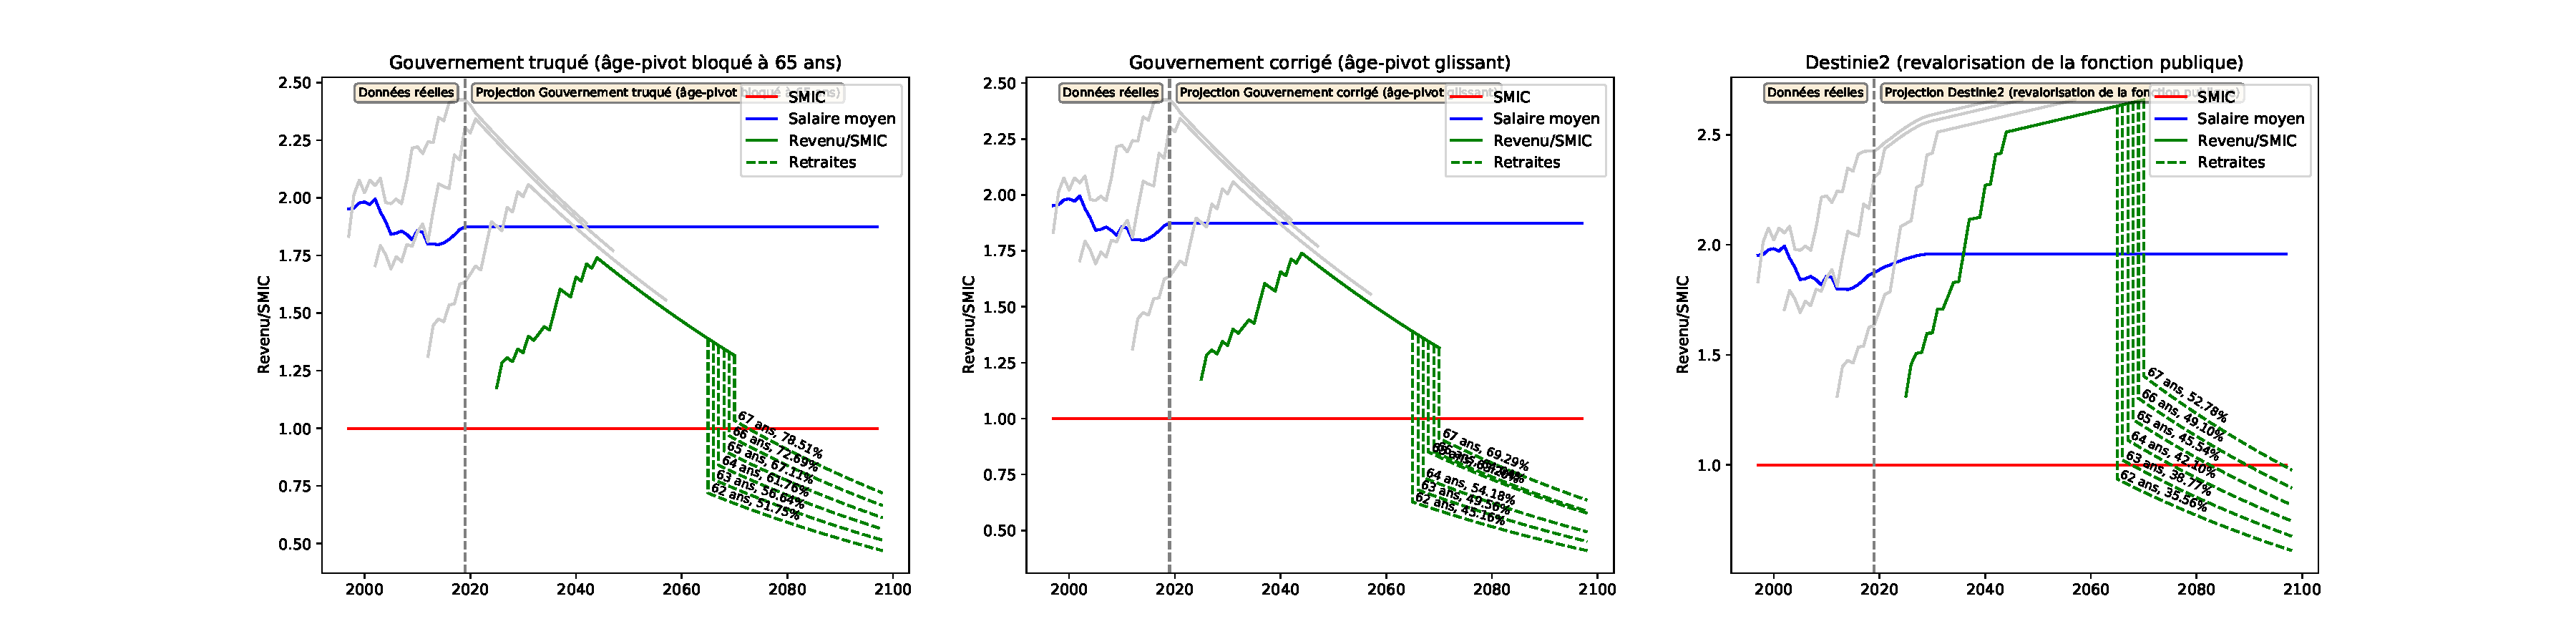
\includegraphics[width=0.9\textwidth]{fig/ProfEcoles_2003_22_dest_retraite.pdf}\end{center} \label{fig/ProfEcoles_2003_22_dest_retraite.pdf} 

\newpage 
 
\chapter{Professeur certifié} 

\begin{minipage}{0.55\linewidth}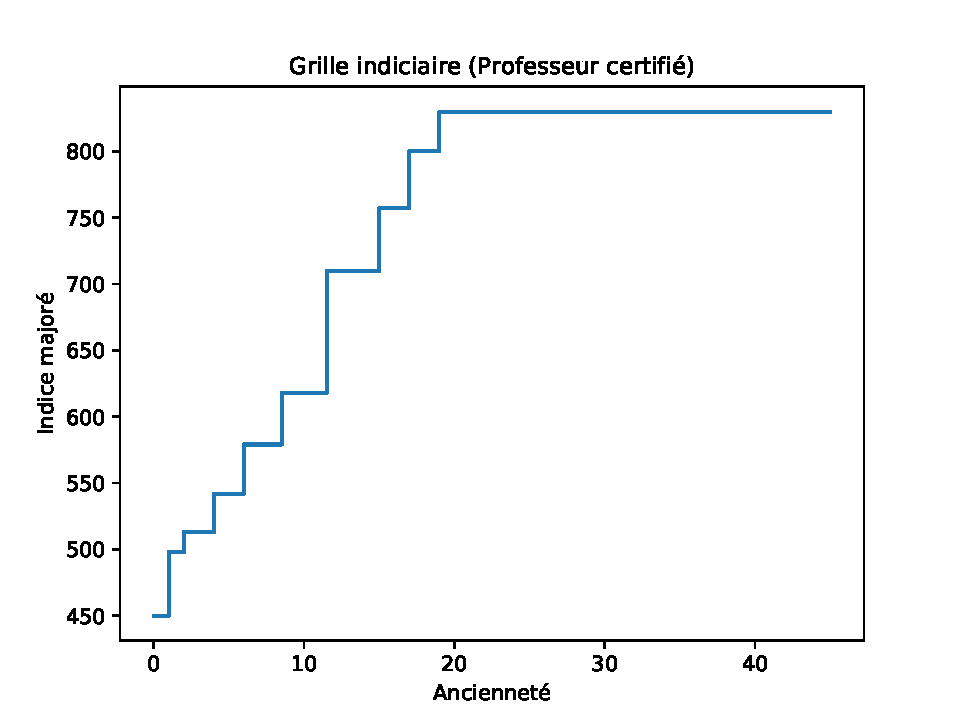
\includegraphics[width=0.7\textwidth]{fig/grille_ProfCertifie.pdf}\end{minipage} 
\begin{minipage}{0.3\linewidth} 
 \begin{center} 

\begin{tabular}[htb]{|c|c|} 
\hline 
 Indice majoré &  Durée (années) \\ 
\hline \hline 
 450 &  1.00 \\ 
\hline 
 498 &  1.00 \\ 
\hline 
 513 &  2.00 \\ 
\hline 
 542 &  2.00 \\ 
\hline 
 579 &  2.50 \\ 
\hline 
 618 &  3.00 \\ 
\hline 
 710 &  3.50 \\ 
\hline 
 757 &  2.00 \\ 
\hline 
 800 &  2.00 \\ 
\hline 
 830 &   \\ 
\hline 
\hline 
\end{tabular} 
\end{center} 
 \end{minipage} 


 \addto{\captionsenglish}{ \renewcommand{\mtctitle}{}} \setcounter{minitocdepth}{2} 
 \minitoc \newpage 

\section{Début de carrière à 22 ans} 

\subsection{Génération 1975 (début en 1997)} 

\paragraph{Retraites possibles et ratios Revenu/SMIC à 70, 75, 80, 85, 90 ans avec le modèle \emph{Gouvernement truqué (âge-pivot bloqué à 65 ans)}}  
 
{ \scriptsize \begin{center} 
\begin{tabular}[htb]{|c|c||c|c||c|c||c||c|c|c|c|c|c|} 
\hline 
 Retraite en &  Âge &  Âge pivot &  Décote/Surcote &  Retraite (\euro{} 2019) &  Tx Rempl(\%) &  SMIC (\euro{} 2019) &  Retraite/SMIC &  Rev70/SMIC &  Rev75/SMIC &  Rev80/SMIC &  Rev85/SMIC &  Rev90/SMIC \\ 
\hline \hline 
 2037 &  62 &  64 ans 10 mois &  -14.17\% &  1927.13 &  {\bf 44.47} &  2143.00 &  {\bf {\color{red} 0.90}} &  {\bf {\color{red} 0.81}} &  {\bf {\color{red} 0.76}} &  {\bf {\color{red} 0.71}} &  {\bf {\color{red} 0.67}} &  {\bf {\color{red} 0.63}} \\ 
\hline 
 2038 &  63 &  64 ans 11 mois &  -9.58\% &  2100.17 &  {\bf 48.36} &  2170.86 &  {\bf {\color{red} 0.97}} &  {\bf {\color{red} 0.88}} &  {\bf {\color{red} 0.83}} &  {\bf {\color{red} 0.78}} &  {\bf {\color{red} 0.73}} &  {\bf {\color{red} 0.68}} \\ 
\hline 
 2039 &  64 &  65 ans 0 mois &  -5.00\% &  2282.71 &  {\bf 52.45} &  2199.08 &  {\bf 1.04} &  {\bf {\color{red} 0.96}} &  {\bf {\color{red} 0.90}} &  {\bf {\color{red} 0.84}} &  {\bf {\color{red} 0.79}} &  {\bf {\color{red} 0.74}} \\ 
\hline 
 2040 &  65 &  65 ans 0 mois &  0.00\% &  2485.56 &  {\bf 56.99} &  2227.67 &  {\bf 1.12} &  {\bf 1.05} &  {\bf {\color{red} 0.98}} &  {\bf {\color{red} 0.92}} &  {\bf {\color{red} 0.86}} &  {\bf {\color{red} 0.81}} \\ 
\hline 
 2041 &  66 &  65 ans 0 mois &  5.00\% &  2699.62 &  {\bf 61.77} &  2256.63 &  {\bf 1.20} &  {\bf 1.14} &  {\bf 1.07} &  {\bf {\color{red} 1.00}} &  {\bf {\color{red} 0.94}} &  {\bf {\color{red} 0.88}} \\ 
\hline 
 2042 &  67 &  65 ans 0 mois &  10.00\% &  2925.48 &  {\bf 66.80} &  2285.97 &  {\bf 1.28} &  {\bf 1.23} &  {\bf 1.15} &  {\bf 1.08} &  {\bf 1.01} &  {\bf {\color{red} 0.95}} \\ 
\hline 
\hline 
\end{tabular} 
\end{center} } 
\paragraph{Retraites possibles et ratios Revenu/SMIC à 70, 75, 80, 85, 90 ans avec le modèle \emph{Gouvernement corrigé (âge-pivot glissant)}}  
 
{ \scriptsize \begin{center} 
\begin{tabular}[htb]{|c|c||c|c||c|c||c||c|c|c|c|c|c|} 
\hline 
 Retraite en &  Âge &  Âge pivot &  Décote/Surcote &  Retraite (\euro{} 2019) &  Tx Rempl(\%) &  SMIC (\euro{} 2019) &  Retraite/SMIC &  Rev70/SMIC &  Rev75/SMIC &  Rev80/SMIC &  Rev85/SMIC &  Rev90/SMIC \\ 
\hline \hline 
 2037 &  62 &  64 ans 10 mois &  -14.17\% &  1927.13 &  {\bf 44.47} &  2143.00 &  {\bf {\color{red} 0.90}} &  {\bf {\color{red} 0.81}} &  {\bf {\color{red} 0.76}} &  {\bf {\color{red} 0.71}} &  {\bf {\color{red} 0.67}} &  {\bf {\color{red} 0.63}} \\ 
\hline 
 2038 &  63 &  64 ans 11 mois &  -9.58\% &  2100.17 &  {\bf 48.36} &  2170.86 &  {\bf {\color{red} 0.97}} &  {\bf {\color{red} 0.88}} &  {\bf {\color{red} 0.83}} &  {\bf {\color{red} 0.78}} &  {\bf {\color{red} 0.73}} &  {\bf {\color{red} 0.68}} \\ 
\hline 
 2039 &  64 &  65 ans 0 mois &  -5.00\% &  2282.71 &  {\bf 52.45} &  2199.08 &  {\bf 1.04} &  {\bf {\color{red} 0.96}} &  {\bf {\color{red} 0.90}} &  {\bf {\color{red} 0.84}} &  {\bf {\color{red} 0.79}} &  {\bf {\color{red} 0.74}} \\ 
\hline 
 2040 &  65 &  65 ans 1 mois &  -0.42\% &  2475.21 &  {\bf 56.75} &  2227.67 &  {\bf 1.11} &  {\bf 1.04} &  {\bf {\color{red} 0.98}} &  {\bf {\color{red} 0.92}} &  {\bf {\color{red} 0.86}} &  {\bf {\color{red} 0.80}} \\ 
\hline 
 2041 &  66 &  65 ans 2 mois &  4.17\% &  2678.20 &  {\bf 61.28} &  2256.63 &  {\bf 1.19} &  {\bf 1.13} &  {\bf 1.06} &  {\bf {\color{red} 0.99}} &  {\bf {\color{red} 0.93}} &  {\bf {\color{red} 0.87}} \\ 
\hline 
 2042 &  67 &  65 ans 3 mois &  8.75\% &  2892.24 &  {\bf 66.04} &  2285.97 &  {\bf 1.27} &  {\bf 1.22} &  {\bf 1.14} &  {\bf 1.07} &  {\bf 1.00} &  {\bf {\color{red} 0.94}} \\ 
\hline 
\hline 
\end{tabular} 
\end{center} } 
\paragraph{Retraites possibles et ratios Revenu/SMIC à 70, 75, 80, 85, 90 ans avec le modèle \emph{Destinie2 (revalorisation de la fonction publique)}}  
 
{ \scriptsize \begin{center} 
\begin{tabular}[htb]{|c|c||c|c||c|c||c||c|c|c|c|c|c|} 
\hline 
 Retraite en &  Âge &  Âge pivot &  Décote/Surcote &  Retraite (\euro{} 2019) &  Tx Rempl(\%) &  SMIC (\euro{} 2019) &  Retraite/SMIC &  Rev70/SMIC &  Rev75/SMIC &  Rev80/SMIC &  Rev85/SMIC &  Rev90/SMIC \\ 
\hline \hline 
 2037 &  62 &  64 ans 10 mois &  -14.17\% &  2131.08 &  {\bf 39.41} &  2014.82 &  {\bf 1.06} &  {\bf {\color{red} 0.95}} &  {\bf {\color{red} 0.89}} &  {\bf {\color{red} 0.84}} &  {\bf {\color{red} 0.79}} &  {\bf {\color{red} 0.74}} \\ 
\hline 
 2038 &  63 &  64 ans 11 mois &  -9.58\% &  2330.95 &  {\bf 42.55} &  2041.01 &  {\bf 1.14} &  {\bf 1.04} &  {\bf {\color{red} 0.98}} &  {\bf {\color{red} 0.92}} &  {\bf {\color{red} 0.86}} &  {\bf {\color{red} 0.81}} \\ 
\hline 
 2039 &  64 &  65 ans 0 mois &  -5.00\% &  2543.05 &  {\bf 45.82} &  2067.55 &  {\bf 1.23} &  {\bf 1.14} &  {\bf 1.07} &  {\bf 1.00} &  {\bf {\color{red} 0.94}} &  {\bf {\color{red} 0.88}} \\ 
\hline 
 2040 &  65 &  65 ans 1 mois &  -0.42\% &  2768.08 &  {\bf 49.24} &  2094.43 &  {\bf 1.32} &  {\bf 1.24} &  {\bf 1.16} &  {\bf 1.09} &  {\bf 1.02} &  {\bf {\color{red} 0.96}} \\ 
\hline 
 2041 &  66 &  65 ans 2 mois &  4.17\% &  3006.79 &  {\bf 52.80} &  2121.65 &  {\bf 1.42} &  {\bf 1.35} &  {\bf 1.26} &  {\bf 1.18} &  {\bf 1.11} &  {\bf 1.04} \\ 
\hline 
 2042 &  67 &  65 ans 3 mois &  8.75\% &  3259.98 &  {\bf 56.51} &  2149.23 &  {\bf 1.52} &  {\bf 1.46} &  {\bf 1.37} &  {\bf 1.28} &  {\bf 1.20} &  {\bf 1.13} \\ 
\hline 
\hline 
\end{tabular} 
\end{center} } 

 \begin{center}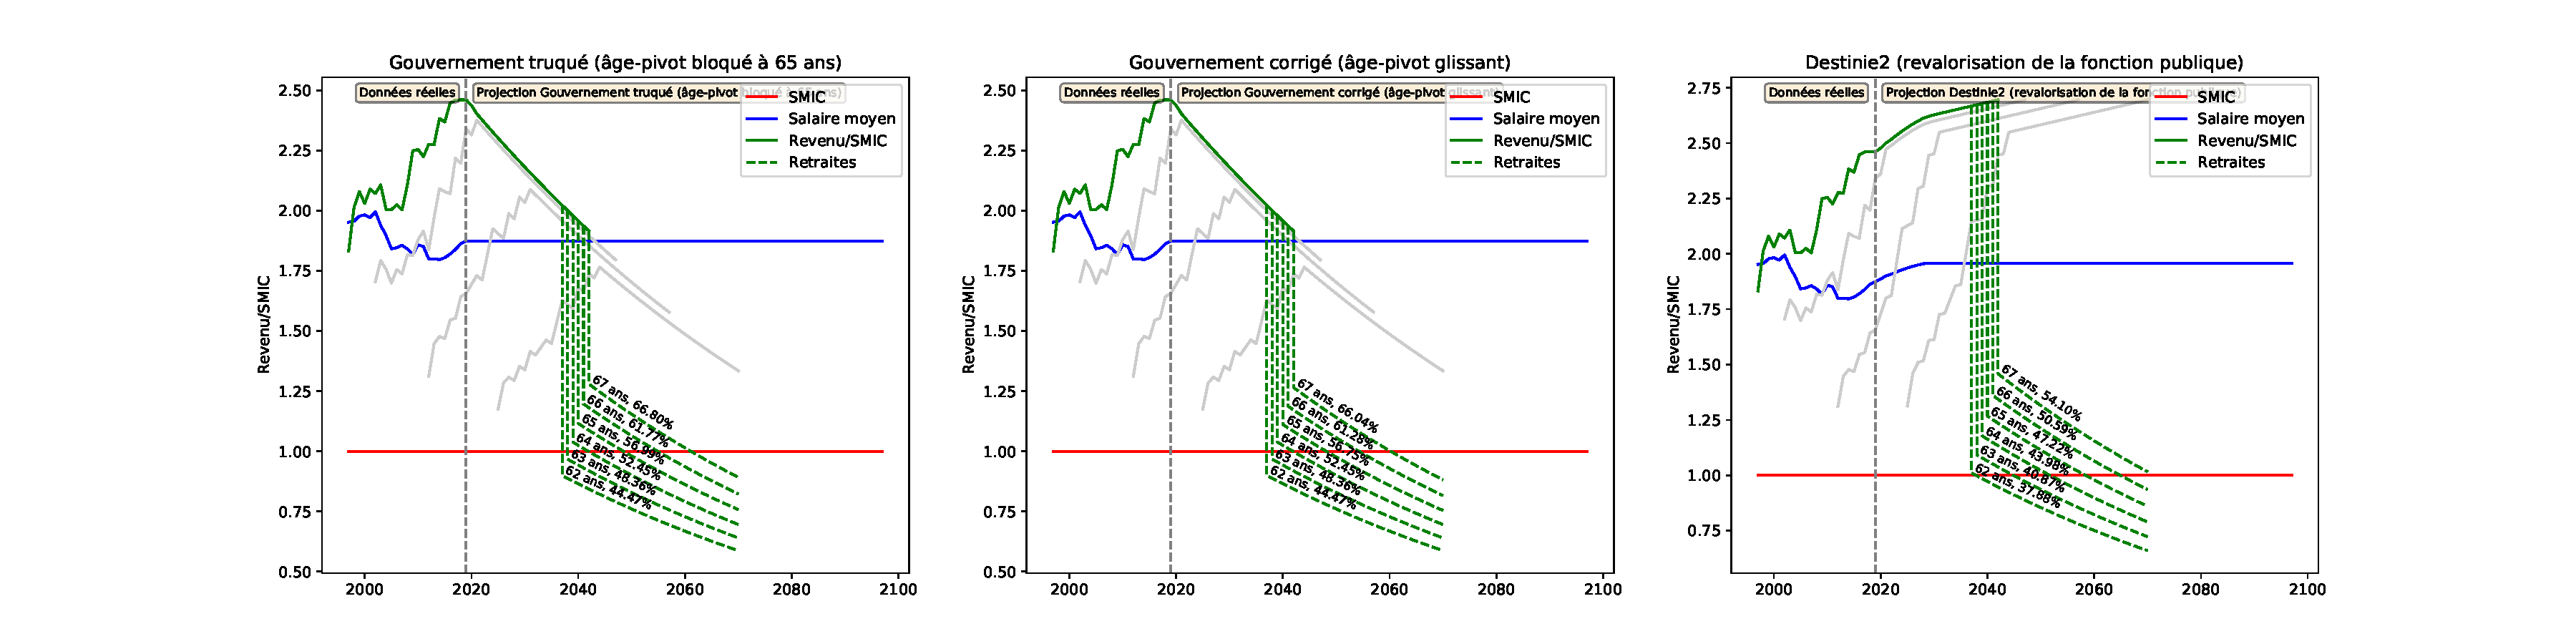
\includegraphics[width=0.9\textwidth]{fig/ProfCertifie_1975_22_dest_retraite.pdf}\end{center} \label{fig/ProfCertifie_1975_22_dest_retraite.pdf} 

\newpage 
 
\subsection{Génération 1980 (début en 2002)} 

\paragraph{Retraites possibles et ratios Revenu/SMIC à 70, 75, 80, 85, 90 ans avec le modèle \emph{Gouvernement truqué (âge-pivot bloqué à 65 ans)}}  
 
{ \scriptsize \begin{center} 
\begin{tabular}[htb]{|c|c||c|c||c|c||c||c|c|c|c|c|c|} 
\hline 
 Retraite en &  Âge &  Âge pivot &  Décote/Surcote &  Retraite (\euro{} 2019) &  Tx Rempl(\%) &  SMIC (\euro{} 2019) &  Retraite/SMIC &  Rev70/SMIC &  Rev75/SMIC &  Rev80/SMIC &  Rev85/SMIC &  Rev90/SMIC \\ 
\hline \hline 
 2042 &  62 &  65 ans 0 mois &  -15.00\% &  1950.60 &  {\bf 45.01} &  2285.97 &  {\bf {\color{red} 0.85}} &  {\bf {\color{red} 0.77}} &  {\bf {\color{red} 0.72}} &  {\bf {\color{red} 0.68}} &  {\bf {\color{red} 0.63}} &  {\bf {\color{red} 0.59}} \\ 
\hline 
 2043 &  63 &  65 ans 0 mois &  -10.00\% &  2143.43 &  {\bf 49.35} &  2315.68 &  {\bf {\color{red} 0.93}} &  {\bf {\color{red} 0.85}} &  {\bf {\color{red} 0.79}} &  {\bf {\color{red} 0.74}} &  {\bf {\color{red} 0.70}} &  {\bf {\color{red} 0.65}} \\ 
\hline 
 2044 &  64 &  65 ans 0 mois &  -5.00\% &  2347.73 &  {\bf 53.94} &  2345.79 &  {\bf 1.00} &  {\bf {\color{red} 0.93}} &  {\bf {\color{red} 0.87}} &  {\bf {\color{red} 0.81}} &  {\bf {\color{red} 0.76}} &  {\bf {\color{red} 0.72}} \\ 
\hline 
 2045 &  65 &  65 ans 0 mois &  0.00\% &  2564.13 &  {\bf 58.79} &  2376.28 &  {\bf 1.08} &  {\bf 1.01} &  {\bf {\color{red} 0.95}} &  {\bf {\color{red} 0.89}} &  {\bf {\color{red} 0.83}} &  {\bf {\color{red} 0.78}} \\ 
\hline 
 2046 &  66 &  65 ans 0 mois &  5.00\% &  2791.21 &  {\bf 63.86} &  2407.18 &  {\bf 1.16} &  {\bf 1.10} &  {\bf 1.03} &  {\bf {\color{red} 0.97}} &  {\bf {\color{red} 0.91}} &  {\bf {\color{red} 0.85}} \\ 
\hline 
 2047 &  67 &  65 ans 0 mois &  10.00\% &  3029.20 &  {\bf 69.16} &  2438.47 &  {\bf 1.24} &  {\bf 1.20} &  {\bf 1.12} &  {\bf 1.05} &  {\bf {\color{red} 0.98}} &  {\bf {\color{red} 0.92}} \\ 
\hline 
\hline 
\end{tabular} 
\end{center} } 
\paragraph{Retraites possibles et ratios Revenu/SMIC à 70, 75, 80, 85, 90 ans avec le modèle \emph{Gouvernement corrigé (âge-pivot glissant)}}  
 
{ \scriptsize \begin{center} 
\begin{tabular}[htb]{|c|c||c|c||c|c||c||c|c|c|c|c|c|} 
\hline 
 Retraite en &  Âge &  Âge pivot &  Décote/Surcote &  Retraite (\euro{} 2019) &  Tx Rempl(\%) &  SMIC (\euro{} 2019) &  Retraite/SMIC &  Rev70/SMIC &  Rev75/SMIC &  Rev80/SMIC &  Rev85/SMIC &  Rev90/SMIC \\ 
\hline \hline 
 2042 &  62 &  65 ans 3 mois &  -16.25\% &  1921.92 &  {\bf 44.35} &  2285.97 &  {\bf {\color{red} 0.84}} &  {\bf {\color{red} 0.76}} &  {\bf {\color{red} 0.71}} &  {\bf {\color{red} 0.67}} &  {\bf {\color{red} 0.62}} &  {\bf {\color{red} 0.59}} \\ 
\hline 
 2043 &  63 &  65 ans 4 mois &  -11.67\% &  2103.73 &  {\bf 48.44} &  2315.68 &  {\bf {\color{red} 0.91}} &  {\bf {\color{red} 0.83}} &  {\bf {\color{red} 0.78}} &  {\bf {\color{red} 0.73}} &  {\bf {\color{red} 0.68}} &  {\bf {\color{red} 0.64}} \\ 
\hline 
 2044 &  64 &  65 ans 5 mois &  -7.08\% &  2296.24 &  {\bf 52.76} &  2345.79 &  {\bf {\color{red} 0.98}} &  {\bf {\color{red} 0.91}} &  {\bf {\color{red} 0.85}} &  {\bf {\color{red} 0.80}} &  {\bf {\color{red} 0.75}} &  {\bf {\color{red} 0.70}} \\ 
\hline 
 2045 &  65 &  65 ans 6 mois &  -2.50\% &  2500.02 &  {\bf 57.32} &  2376.28 &  {\bf 1.05} &  {\bf {\color{red} 0.99}} &  {\bf {\color{red} 0.92}} &  {\bf {\color{red} 0.87}} &  {\bf {\color{red} 0.81}} &  {\bf {\color{red} 0.76}} \\ 
\hline 
 2046 &  66 &  65 ans 7 mois &  2.08\% &  2713.68 &  {\bf 62.09} &  2407.18 &  {\bf 1.13} &  {\bf 1.07} &  {\bf 1.00} &  {\bf {\color{red} 0.94}} &  {\bf {\color{red} 0.88}} &  {\bf {\color{red} 0.83}} \\ 
\hline 
 2047 &  67 &  65 ans 8 mois &  6.67\% &  2937.40 &  {\bf 67.07} &  2438.47 &  {\bf 1.20} &  {\bf 1.16} &  {\bf 1.09} &  {\bf 1.02} &  {\bf {\color{red} 0.95}} &  {\bf {\color{red} 0.90}} \\ 
\hline 
\hline 
\end{tabular} 
\end{center} } 
\paragraph{Retraites possibles et ratios Revenu/SMIC à 70, 75, 80, 85, 90 ans avec le modèle \emph{Destinie2 (revalorisation de la fonction publique)}}  
 
{ \scriptsize \begin{center} 
\begin{tabular}[htb]{|c|c||c|c||c|c||c||c|c|c|c|c|c|} 
\hline 
 Retraite en &  Âge &  Âge pivot &  Décote/Surcote &  Retraite (\euro{} 2019) &  Tx Rempl(\%) &  SMIC (\euro{} 2019) &  Retraite/SMIC &  Rev70/SMIC &  Rev75/SMIC &  Rev80/SMIC &  Rev85/SMIC &  Rev90/SMIC \\ 
\hline \hline 
 2042 &  62 &  65 ans 3 mois &  -16.25\% &  2201.71 &  {\bf 38.17} &  2149.23 &  {\bf 1.02} &  {\bf {\color{red} 0.92}} &  {\bf {\color{red} 0.87}} &  {\bf {\color{red} 0.81}} &  {\bf {\color{red} 0.76}} &  {\bf {\color{red} 0.71}} \\ 
\hline 
 2043 &  63 &  65 ans 4 mois &  -11.67\% &  2420.67 &  {\bf 41.42} &  2177.17 &  {\bf 1.11} &  {\bf 1.02} &  {\bf {\color{red} 0.95}} &  {\bf {\color{red} 0.89}} &  {\bf {\color{red} 0.84}} &  {\bf {\color{red} 0.78}} \\ 
\hline 
 2044 &  64 &  65 ans 5 mois &  -7.08\% &  2653.98 &  {\bf 44.83} &  2205.48 &  {\bf 1.20} &  {\bf 1.11} &  {\bf 1.04} &  {\bf {\color{red} 0.98}} &  {\bf {\color{red} 0.92}} &  {\bf {\color{red} 0.86}} \\ 
\hline 
 2045 &  65 &  65 ans 6 mois &  -2.50\% &  2902.48 &  {\bf 48.40} &  2234.15 &  {\bf 1.30} &  {\bf 1.22} &  {\bf 1.14} &  {\bf 1.07} &  {\bf 1.00} &  {\bf {\color{red} 0.94}} \\ 
\hline 
 2046 &  66 &  65 ans 7 mois &  2.08\% &  3164.75 &  {\bf 52.10} &  2263.19 &  {\bf 1.40} &  {\bf 1.33} &  {\bf 1.24} &  {\bf 1.17} &  {\bf 1.09} &  {\bf 1.03} \\ 
\hline 
 2047 &  67 &  65 ans 8 mois &  6.67\% &  3441.19 &  {\bf 55.92} &  2292.61 &  {\bf 1.50} &  {\bf 1.44} &  {\bf 1.35} &  {\bf 1.27} &  {\bf 1.19} &  {\bf 1.12} \\ 
\hline 
\hline 
\end{tabular} 
\end{center} } 

 \begin{center}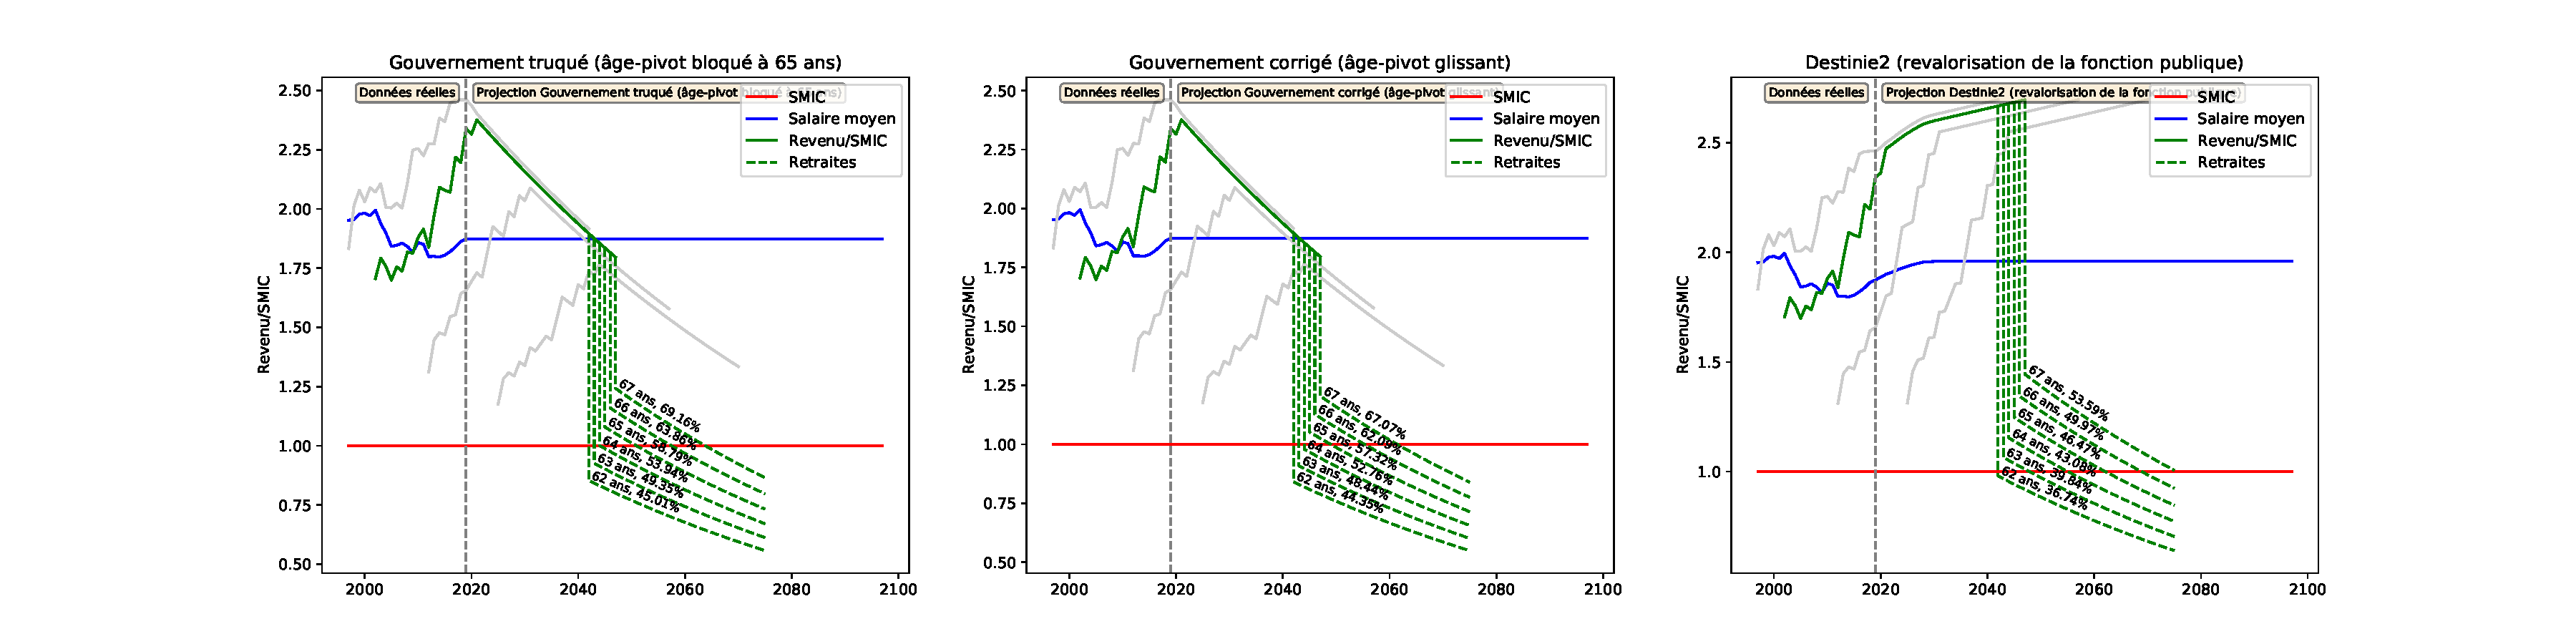
\includegraphics[width=0.9\textwidth]{fig/ProfCertifie_1980_22_dest_retraite.pdf}\end{center} \label{fig/ProfCertifie_1980_22_dest_retraite.pdf} 

\newpage 
 
\subsection{Génération 1990 (début en 2012)} 

\paragraph{Retraites possibles et ratios Revenu/SMIC à 70, 75, 80, 85, 90 ans avec le modèle \emph{Gouvernement truqué (âge-pivot bloqué à 65 ans)}}  
 
{ \scriptsize \begin{center} 
\begin{tabular}[htb]{|c|c||c|c||c|c||c||c|c|c|c|c|c|} 
\hline 
 Retraite en &  Âge &  Âge pivot &  Décote/Surcote &  Retraite (\euro{} 2019) &  Tx Rempl(\%) &  SMIC (\euro{} 2019) &  Retraite/SMIC &  Rev70/SMIC &  Rev75/SMIC &  Rev80/SMIC &  Rev85/SMIC &  Rev90/SMIC \\ 
\hline \hline 
 2052 &  62 &  65 ans 0 mois &  -15.00\% &  2096.42 &  {\bf 48.37} &  2601.14 &  {\bf {\color{red} 0.81}} &  {\bf {\color{red} 0.73}} &  {\bf {\color{red} 0.68}} &  {\bf {\color{red} 0.64}} &  {\bf {\color{red} 0.60}} &  {\bf {\color{red} 0.56}} \\ 
\hline 
 2053 &  63 &  65 ans 0 mois &  -10.00\% &  2303.01 &  {\bf 53.03} &  2634.96 &  {\bf {\color{red} 0.87}} &  {\bf {\color{red} 0.80}} &  {\bf {\color{red} 0.75}} &  {\bf {\color{red} 0.70}} &  {\bf {\color{red} 0.66}} &  {\bf {\color{red} 0.62}} \\ 
\hline 
 2054 &  64 &  65 ans 0 mois &  -5.00\% &  2520.11 &  {\bf 57.90} &  2669.21 &  {\bf {\color{red} 0.94}} &  {\bf {\color{red} 0.87}} &  {\bf {\color{red} 0.82}} &  {\bf {\color{red} 0.77}} &  {\bf {\color{red} 0.72}} &  {\bf {\color{red} 0.67}} \\ 
\hline 
 2055 &  65 &  65 ans 0 mois &  0.00\% &  2747.94 &  {\bf 63.01} &  2703.91 &  {\bf 1.02} &  {\bf {\color{red} 0.95}} &  {\bf {\color{red} 0.89}} &  {\bf {\color{red} 0.84}} &  {\bf {\color{red} 0.78}} &  {\bf {\color{red} 0.74}} \\ 
\hline 
 2056 &  66 &  65 ans 0 mois &  5.00\% &  2986.72 &  {\bf 68.34} &  2739.06 &  {\bf 1.09} &  {\bf 1.04} &  {\bf {\color{red} 0.97}} &  {\bf {\color{red} 0.91}} &  {\bf {\color{red} 0.85}} &  {\bf {\color{red} 0.80}} \\ 
\hline 
 2057 &  67 &  65 ans 0 mois &  10.00\% &  3236.68 &  {\bf 73.90} &  2774.67 &  {\bf 1.17} &  {\bf 1.12} &  {\bf 1.05} &  {\bf {\color{red} 0.99}} &  {\bf {\color{red} 0.92}} &  {\bf {\color{red} 0.87}} \\ 
\hline 
\hline 
\end{tabular} 
\end{center} } 
\paragraph{Retraites possibles et ratios Revenu/SMIC à 70, 75, 80, 85, 90 ans avec le modèle \emph{Gouvernement corrigé (âge-pivot glissant)}}  
 
{ \scriptsize \begin{center} 
\begin{tabular}[htb]{|c|c||c|c||c|c||c||c|c|c|c|c|c|} 
\hline 
 Retraite en &  Âge &  Âge pivot &  Décote/Surcote &  Retraite (\euro{} 2019) &  Tx Rempl(\%) &  SMIC (\euro{} 2019) &  Retraite/SMIC &  Rev70/SMIC &  Rev75/SMIC &  Rev80/SMIC &  Rev85/SMIC &  Rev90/SMIC \\ 
\hline \hline 
 2052 &  62 &  66 ans 1 mois &  -20.42\% &  1962.83 &  {\bf 45.29} &  2601.14 &  {\bf {\color{red} 0.75}} &  {\bf {\color{red} 0.68}} &  {\bf {\color{red} 0.64}} &  {\bf {\color{red} 0.60}} &  {\bf {\color{red} 0.56}} &  {\bf {\color{red} 0.53}} \\ 
\hline 
 2053 &  63 &  66 ans 2 mois &  -15.83\% &  2153.74 &  {\bf 49.59} &  2634.96 &  {\bf {\color{red} 0.82}} &  {\bf {\color{red} 0.75}} &  {\bf {\color{red} 0.70}} &  {\bf {\color{red} 0.66}} &  {\bf {\color{red} 0.62}} &  {\bf {\color{red} 0.58}} \\ 
\hline 
 2054 &  64 &  66 ans 3 mois &  -11.25\% &  2354.31 &  {\bf 54.09} &  2669.21 &  {\bf {\color{red} 0.88}} &  {\bf {\color{red} 0.82}} &  {\bf {\color{red} 0.77}} &  {\bf {\color{red} 0.72}} &  {\bf {\color{red} 0.67}} &  {\bf {\color{red} 0.63}} \\ 
\hline 
 2055 &  65 &  66 ans 4 mois &  -6.67\% &  2564.74 &  {\bf 58.81} &  2703.91 &  {\bf {\color{red} 0.95}} &  {\bf {\color{red} 0.89}} &  {\bf {\color{red} 0.83}} &  {\bf {\color{red} 0.78}} &  {\bf {\color{red} 0.73}} &  {\bf {\color{red} 0.69}} \\ 
\hline 
 2056 &  66 &  66 ans 5 mois &  -2.08\% &  2785.23 &  {\bf 63.73} &  2739.06 &  {\bf 1.02} &  {\bf {\color{red} 0.97}} &  {\bf {\color{red} 0.91}} &  {\bf {\color{red} 0.85}} &  {\bf {\color{red} 0.80}} &  {\bf {\color{red} 0.75}} \\ 
\hline 
 2057 &  67 &  66 ans 6 mois &  2.50\% &  3016.00 &  {\bf 68.86} &  2774.67 &  {\bf 1.09} &  {\bf 1.05} &  {\bf {\color{red} 0.98}} &  {\bf {\color{red} 0.92}} &  {\bf {\color{red} 0.86}} &  {\bf {\color{red} 0.81}} \\ 
\hline 
\hline 
\end{tabular} 
\end{center} } 
\paragraph{Retraites possibles et ratios Revenu/SMIC à 70, 75, 80, 85, 90 ans avec le modèle \emph{Destinie2 (revalorisation de la fonction publique)}}  
 
{ \scriptsize \begin{center} 
\begin{tabular}[htb]{|c|c||c|c||c|c||c||c|c|c|c|c|c|} 
\hline 
 Retraite en &  Âge &  Âge pivot &  Décote/Surcote &  Retraite (\euro{} 2019) &  Tx Rempl(\%) &  SMIC (\euro{} 2019) &  Retraite/SMIC &  Rev70/SMIC &  Rev75/SMIC &  Rev80/SMIC &  Rev85/SMIC &  Rev90/SMIC \\ 
\hline \hline 
 2052 &  62 &  66 ans 1 mois &  -20.42\% &  2470.63 &  {\bf 37.64} &  2445.56 &  {\bf 1.01} &  {\bf {\color{red} 0.91}} &  {\bf {\color{red} 0.85}} &  {\bf {\color{red} 0.80}} &  {\bf {\color{red} 0.75}} &  {\bf {\color{red} 0.70}} \\ 
\hline 
 2053 &  63 &  66 ans 2 mois &  -15.83\% &  2724.79 &  {\bf 40.98} &  2477.35 &  {\bf 1.10} &  {\bf 1.00} &  {\bf {\color{red} 0.94}} &  {\bf {\color{red} 0.88}} &  {\bf {\color{red} 0.83}} &  {\bf {\color{red} 0.78}} \\ 
\hline 
 2054 &  64 &  66 ans 3 mois &  -11.25\% &  2993.73 &  {\bf 44.44} &  2509.56 &  {\bf 1.19} &  {\bf 1.10} &  {\bf 1.03} &  {\bf {\color{red} 0.97}} &  {\bf {\color{red} 0.91}} &  {\bf {\color{red} 0.85}} \\ 
\hline 
 2055 &  65 &  66 ans 4 mois &  -6.67\% &  3277.91 &  {\bf 48.04} &  2542.18 &  {\bf 1.29} &  {\bf 1.21} &  {\bf 1.13} &  {\bf 1.06} &  {\bf {\color{red} 1.00}} &  {\bf {\color{red} 0.93}} \\ 
\hline 
 2056 &  66 &  66 ans 5 mois &  -2.08\% &  3577.80 &  {\bf 51.76} &  2575.23 &  {\bf 1.39} &  {\bf 1.32} &  {\bf 1.24} &  {\bf 1.16} &  {\bf 1.09} &  {\bf 1.02} \\ 
\hline 
 2057 &  67 &  66 ans 6 mois &  2.50\% &  3893.86 &  {\bf 55.61} &  2608.71 &  {\bf 1.49} &  {\bf 1.44} &  {\bf 1.35} &  {\bf 1.26} &  {\bf 1.18} &  {\bf 1.11} \\ 
\hline 
\hline 
\end{tabular} 
\end{center} } 

 \begin{center}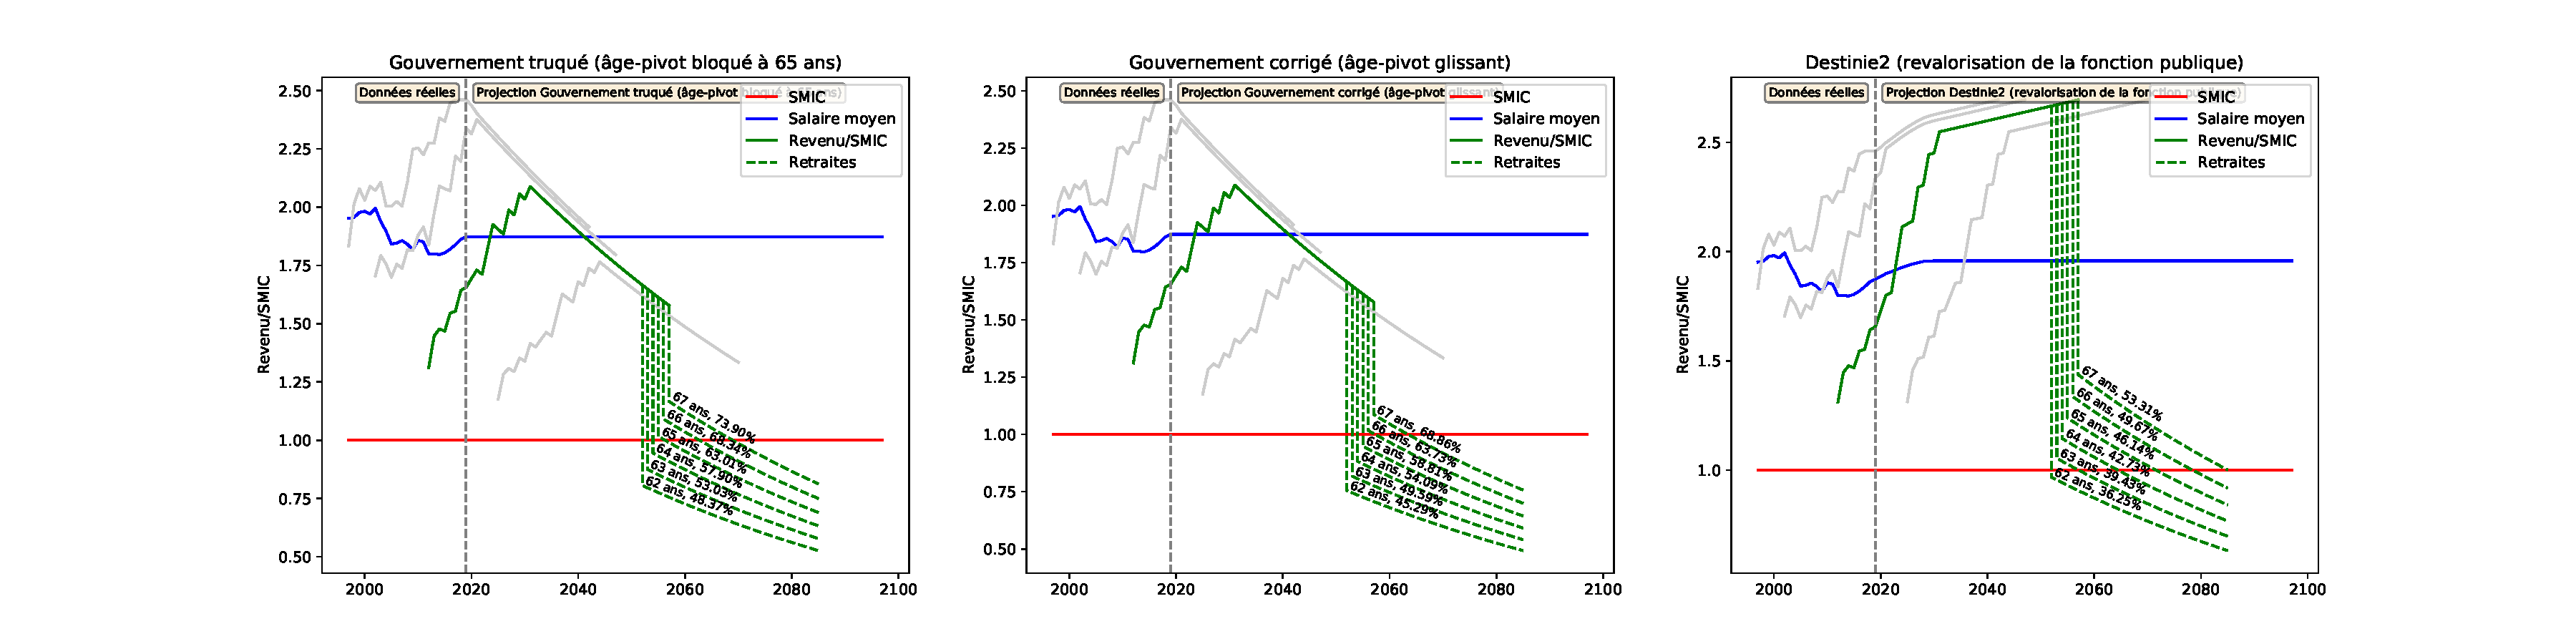
\includegraphics[width=0.9\textwidth]{fig/ProfCertifie_1990_22_dest_retraite.pdf}\end{center} \label{fig/ProfCertifie_1990_22_dest_retraite.pdf} 

\newpage 
 
\subsection{Génération 2003 (début en 2025)} 

\paragraph{Retraites possibles et ratios Revenu/SMIC à 70, 75, 80, 85, 90 ans avec le modèle \emph{Gouvernement truqué (âge-pivot bloqué à 65 ans)}}  
 
{ \scriptsize \begin{center} 
\begin{tabular}[htb]{|c|c||c|c||c|c||c||c|c|c|c|c|c|} 
\hline 
 Retraite en &  Âge &  Âge pivot &  Décote/Surcote &  Retraite (\euro{} 2019) &  Tx Rempl(\%) &  SMIC (\euro{} 2019) &  Retraite/SMIC &  Rev70/SMIC &  Rev75/SMIC &  Rev80/SMIC &  Rev85/SMIC &  Rev90/SMIC \\ 
\hline \hline 
 2065 &  62 &  65 ans 0 mois &  -15.00\% &  2241.05 &  {\bf 51.71} &  3076.71 &  {\bf {\color{red} 0.73}} &  {\bf {\color{red} 0.66}} &  {\bf {\color{red} 0.62}} &  {\bf {\color{red} 0.58}} &  {\bf {\color{red} 0.54}} &  {\bf {\color{red} 0.51}} \\ 
\hline 
 2066 &  63 &  65 ans 0 mois &  -10.00\% &  2458.13 &  {\bf 56.60} &  3116.71 &  {\bf {\color{red} 0.79}} &  {\bf {\color{red} 0.72}} &  {\bf {\color{red} 0.68}} &  {\bf {\color{red} 0.63}} &  {\bf {\color{red} 0.59}} &  {\bf {\color{red} 0.56}} \\ 
\hline 
 2067 &  64 &  65 ans 0 mois &  -5.00\% &  2685.98 &  {\bf 61.71} &  3157.23 &  {\bf {\color{red} 0.85}} &  {\bf {\color{red} 0.79}} &  {\bf {\color{red} 0.74}} &  {\bf {\color{red} 0.69}} &  {\bf {\color{red} 0.65}} &  {\bf {\color{red} 0.61}} \\ 
\hline 
 2068 &  65 &  65 ans 0 mois &  0.00\% &  2924.81 &  {\bf 67.06} &  3198.27 &  {\bf {\color{red} 0.91}} &  {\bf {\color{red} 0.86}} &  {\bf {\color{red} 0.80}} &  {\bf {\color{red} 0.75}} &  {\bf {\color{red} 0.71}} &  {\bf {\color{red} 0.66}} \\ 
\hline 
 2069 &  66 &  65 ans 0 mois &  5.00\% &  3174.85 &  {\bf 72.64} &  3239.85 &  {\bf {\color{red} 0.98}} &  {\bf {\color{red} 0.93}} &  {\bf {\color{red} 0.87}} &  {\bf {\color{red} 0.82}} &  {\bf {\color{red} 0.77}} &  {\bf {\color{red} 0.72}} \\ 
\hline 
 2070 &  67 &  65 ans 0 mois &  10.00\% &  3436.33 &  {\bf 78.46} &  3281.97 &  {\bf 1.05} &  {\bf 1.01} &  {\bf {\color{red} 0.94}} &  {\bf {\color{red} 0.89}} &  {\bf {\color{red} 0.83}} &  {\bf {\color{red} 0.78}} \\ 
\hline 
\hline 
\end{tabular} 
\end{center} } 
\paragraph{Retraites possibles et ratios Revenu/SMIC à 70, 75, 80, 85, 90 ans avec le modèle \emph{Gouvernement corrigé (âge-pivot glissant)}}  
 
{ \scriptsize \begin{center} 
\begin{tabular}[htb]{|c|c||c|c||c|c||c||c|c|c|c|c|c|} 
\hline 
 Retraite en &  Âge &  Âge pivot &  Décote/Surcote &  Retraite (\euro{} 2019) &  Tx Rempl(\%) &  SMIC (\euro{} 2019) &  Retraite/SMIC &  Rev70/SMIC &  Rev75/SMIC &  Rev80/SMIC &  Rev85/SMIC &  Rev90/SMIC \\ 
\hline \hline 
 2065 &  62 &  67 ans 2 mois &  -25.83\% &  1955.43 &  {\bf 45.12} &  3076.71 &  {\bf {\color{red} 0.64}} &  {\bf {\color{red} 0.57}} &  {\bf {\color{red} 0.54}} &  {\bf {\color{red} 0.50}} &  {\bf {\color{red} 0.47}} &  {\bf {\color{red} 0.44}} \\ 
\hline 
 2066 &  63 &  67 ans 3 mois &  -21.25\% &  2150.87 &  {\bf 49.52} &  3116.71 &  {\bf {\color{red} 0.69}} &  {\bf {\color{red} 0.63}} &  {\bf {\color{red} 0.59}} &  {\bf {\color{red} 0.55}} &  {\bf {\color{red} 0.52}} &  {\bf {\color{red} 0.49}} \\ 
\hline 
 2067 &  64 &  67 ans 4 mois &  -16.67\% &  2356.12 &  {\bf 54.14} &  3157.23 &  {\bf {\color{red} 0.75}} &  {\bf {\color{red} 0.69}} &  {\bf {\color{red} 0.65}} &  {\bf {\color{red} 0.61}} &  {\bf {\color{red} 0.57}} &  {\bf {\color{red} 0.53}} \\ 
\hline 
 2068 &  65 &  67 ans 5 mois &  -12.08\% &  2718.53 &  {\bf 62.33} &  3198.27 &  {\bf {\color{red} 0.85}} &  {\bf {\color{red} 0.80}} &  {\bf {\color{red} 0.75}} &  {\bf {\color{red} 0.70}} &  {\bf {\color{red} 0.66}} &  {\bf {\color{red} 0.62}} \\ 
\hline 
 2069 &  66 &  67 ans 6 mois &  -7.50\% &  2796.89 &  {\bf 63.99} &  3239.85 &  {\bf {\color{red} 0.86}} &  {\bf {\color{red} 0.82}} &  {\bf {\color{red} 0.77}} &  {\bf {\color{red} 0.72}} &  {\bf {\color{red} 0.68}} &  {\bf {\color{red} 0.63}} \\ 
\hline 
 2070 &  67 &  67 ans 7 mois &  -2.92\% &  3032.82 &  {\bf 69.25} &  3281.97 &  {\bf {\color{red} 0.92}} &  {\bf {\color{red} 0.89}} &  {\bf {\color{red} 0.83}} &  {\bf {\color{red} 0.78}} &  {\bf {\color{red} 0.73}} &  {\bf {\color{red} 0.69}} \\ 
\hline 
\hline 
\end{tabular} 
\end{center} } 
\paragraph{Retraites possibles et ratios Revenu/SMIC à 70, 75, 80, 85, 90 ans avec le modèle \emph{Destinie2 (revalorisation de la fonction publique)}}  
 
{ \scriptsize \begin{center} 
\begin{tabular}[htb]{|c|c||c|c||c|c||c||c|c|c|c|c|c|} 
\hline 
 Retraite en &  Âge &  Âge pivot &  Décote/Surcote &  Retraite (\euro{} 2019) &  Tx Rempl(\%) &  SMIC (\euro{} 2019) &  Retraite/SMIC &  Rev70/SMIC &  Rev75/SMIC &  Rev80/SMIC &  Rev85/SMIC &  Rev90/SMIC \\ 
\hline \hline 
 2065 &  62 &  67 ans 2 mois &  -25.83\% &  2867.77 &  {\bf 36.94} &  2892.68 &  {\bf {\color{red} 0.99}} &  {\bf {\color{red} 0.89}} &  {\bf {\color{red} 0.84}} &  {\bf {\color{red} 0.79}} &  {\bf {\color{red} 0.74}} &  {\bf {\color{red} 0.69}} \\ 
\hline 
 2066 &  63 &  67 ans 3 mois &  -21.25\% &  3170.80 &  {\bf 40.31} &  2930.29 &  {\bf 1.08} &  {\bf {\color{red} 0.99}} &  {\bf {\color{red} 0.93}} &  {\bf {\color{red} 0.87}} &  {\bf {\color{red} 0.81}} &  {\bf {\color{red} 0.76}} \\ 
\hline 
 2067 &  64 &  67 ans 4 mois &  -16.67\% &  3491.38 &  {\bf 43.82} &  2968.38 &  {\bf 1.18} &  {\bf 1.09} &  {\bf 1.02} &  {\bf {\color{red} 0.96}} &  {\bf {\color{red} 0.90}} &  {\bf {\color{red} 0.84}} \\ 
\hline 
 2068 &  65 &  67 ans 5 mois &  -12.08\% &  3830.06 &  {\bf 47.45} &  3006.97 &  {\bf 1.27} &  {\bf 1.19} &  {\bf 1.12} &  {\bf 1.05} &  {\bf {\color{red} 0.98}} &  {\bf {\color{red} 0.92}} \\ 
\hline 
 2069 &  66 &  67 ans 6 mois &  -7.50\% &  4187.38 &  {\bf 51.22} &  3046.06 &  {\bf 1.37} &  {\bf 1.31} &  {\bf 1.22} &  {\bf 1.15} &  {\bf 1.08} &  {\bf 1.01} \\ 
\hline 
 2070 &  67 &  67 ans 7 mois &  -2.92\% &  4563.92 &  {\bf 55.10} &  3085.66 &  {\bf 1.48} &  {\bf 1.42} &  {\bf 1.33} &  {\bf 1.25} &  {\bf 1.17} &  {\bf 1.10} \\ 
\hline 
\hline 
\end{tabular} 
\end{center} } 

 \begin{center}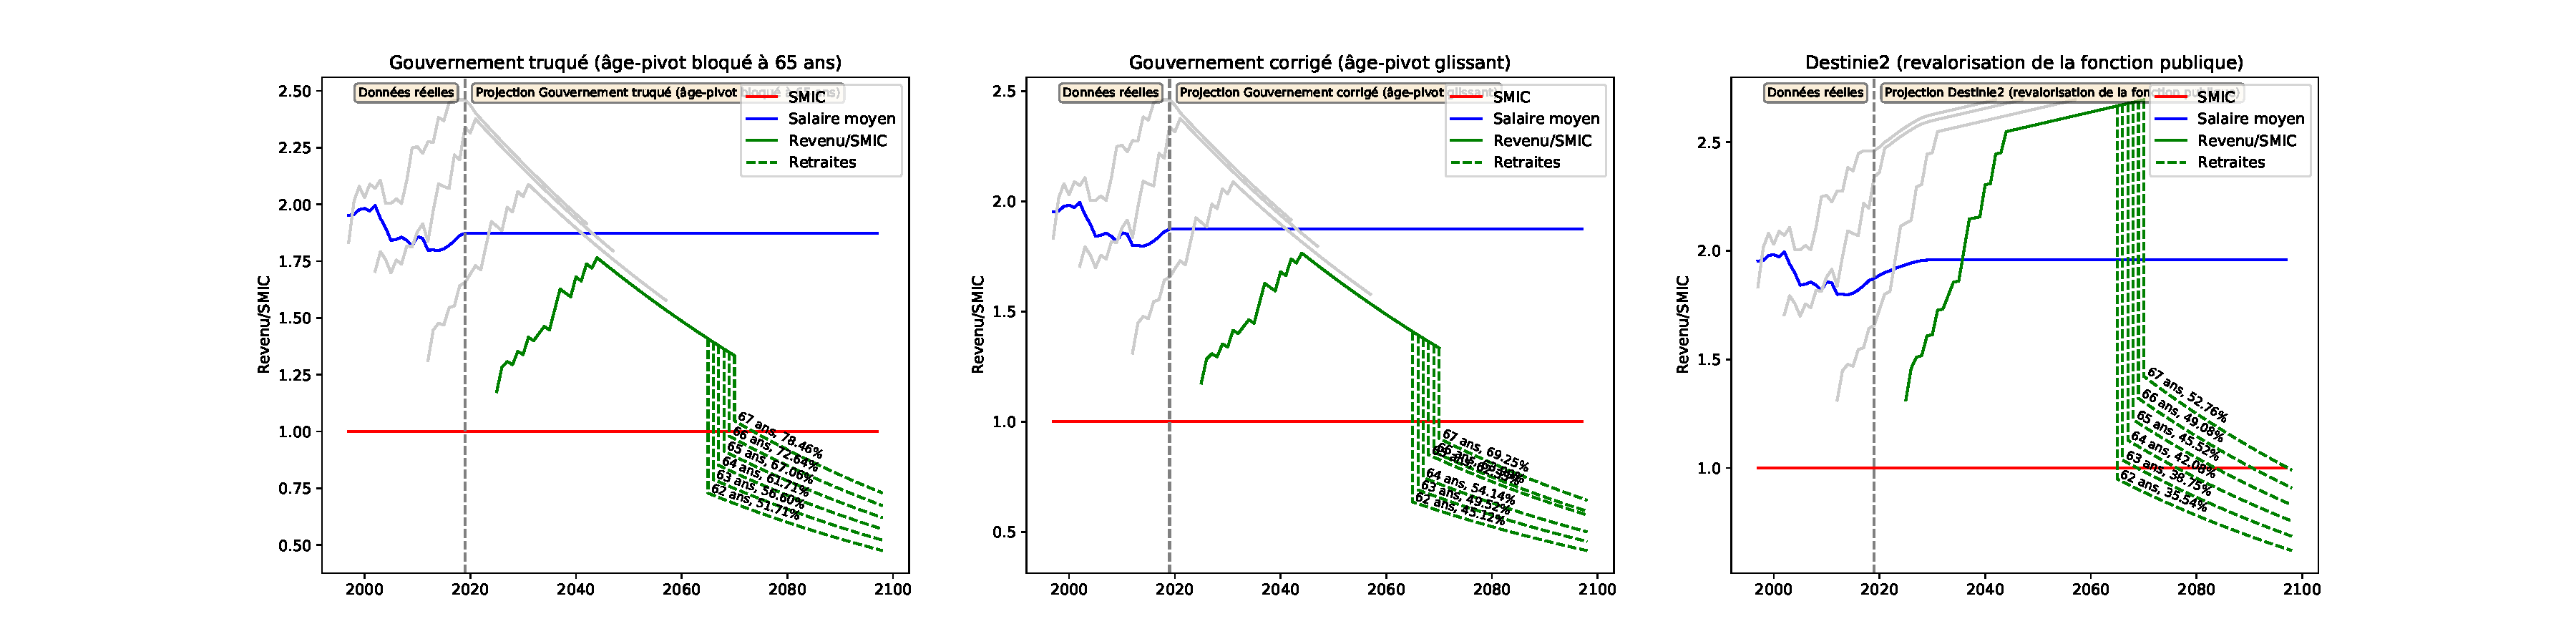
\includegraphics[width=0.9\textwidth]{fig/ProfCertifie_2003_22_dest_retraite.pdf}\end{center} \label{fig/ProfCertifie_2003_22_dest_retraite.pdf} 

\newpage 
 
\chapter{Professeur agrégé} 

\begin{minipage}{0.55\linewidth}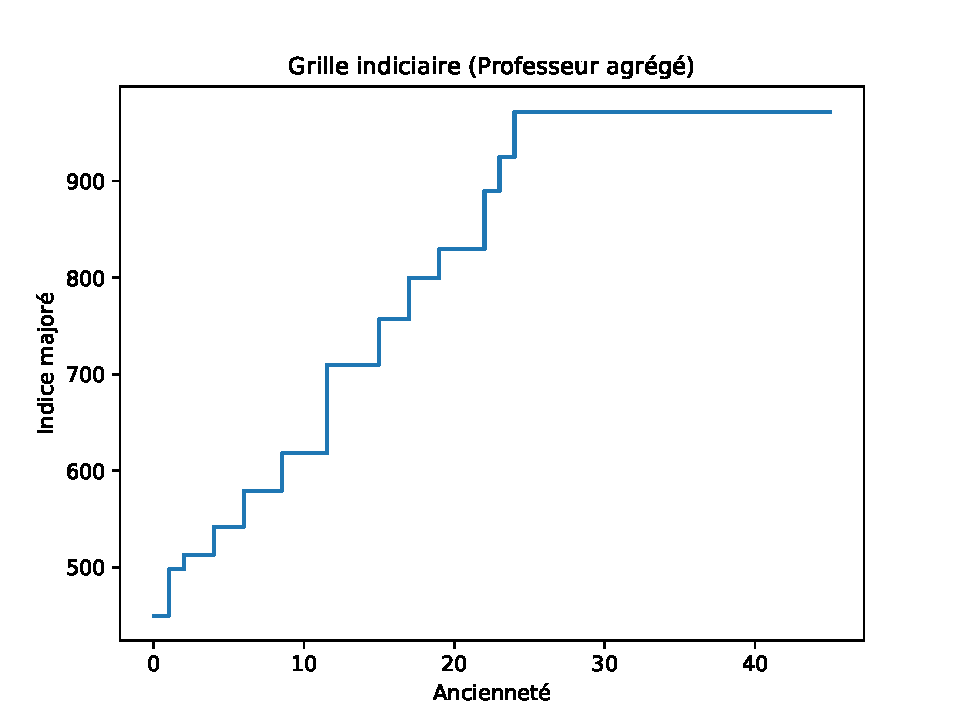
\includegraphics[width=0.7\textwidth]{fig/grille_ProfAgrege.pdf}\end{minipage} 
\begin{minipage}{0.3\linewidth} 
 \begin{center} 

\begin{tabular}[htb]{|c|c|} 
\hline 
 Indice majoré &  Durée (années) \\ 
\hline \hline 
 450 &  1.00 \\ 
\hline 
 498 &  1.00 \\ 
\hline 
 513 &  2.00 \\ 
\hline 
 542 &  2.00 \\ 
\hline 
 579 &  2.50 \\ 
\hline 
 618 &  3.00 \\ 
\hline 
 710 &  3.50 \\ 
\hline 
 757 &  2.00 \\ 
\hline 
 800 &  2.00 \\ 
\hline 
 830 &  3.00 \\ 
\hline 
 890 &  1.00 \\ 
\hline 
 925 &  1.00 \\ 
\hline 
 972 &   \\ 
\hline 
\hline 
\end{tabular} 
\end{center} 
 \end{minipage} 


 \addto{\captionsenglish}{ \renewcommand{\mtctitle}{}} \setcounter{minitocdepth}{2} 
 \minitoc \newpage 

\section{Début de carrière à 22 ans} 

\subsection{Génération 1975 (début en 1997)} 

\paragraph{Retraites possibles et ratios Revenu/SMIC à 70, 75, 80, 85, 90 ans avec le modèle \emph{Gouvernement truqué (âge-pivot bloqué à 65 ans)}}  
 
{ \scriptsize \begin{center} 
\begin{tabular}[htb]{|c|c||c|c||c|c||c||c|c|c|c|c|c|} 
\hline 
 Retraite en &  Âge &  Âge pivot &  Décote/Surcote &  Retraite (\euro{} 2019) &  Tx Rempl(\%) &  SMIC (\euro{} 2019) &  Retraite/SMIC &  Rev70/SMIC &  Rev75/SMIC &  Rev80/SMIC &  Rev85/SMIC &  Rev90/SMIC \\ 
\hline \hline 
 2037 &  62 &  64 ans 10 mois &  -14.17\% &  2088.51 &  {\bf 41.15} &  2143.00 &  {\bf {\color{red} 0.97}} &  {\bf {\color{red} 0.88}} &  {\bf {\color{red} 0.82}} &  {\bf {\color{red} 0.77}} &  {\bf {\color{red} 0.72}} &  {\bf {\color{red} 0.68}} \\ 
\hline 
 2038 &  63 &  64 ans 11 mois &  -9.58\% &  2280.82 &  {\bf 44.84} &  2170.86 &  {\bf 1.05} &  {\bf {\color{red} 0.96}} &  {\bf {\color{red} 0.90}} &  {\bf {\color{red} 0.84}} &  {\bf {\color{red} 0.79}} &  {\bf {\color{red} 0.74}} \\ 
\hline 
 2039 &  64 &  65 ans 0 mois &  -5.00\% &  2483.95 &  {\bf 48.74} &  2199.08 &  {\bf 1.13} &  {\bf 1.05} &  {\bf {\color{red} 0.98}} &  {\bf {\color{red} 0.92}} &  {\bf {\color{red} 0.86}} &  {\bf {\color{red} 0.81}} \\ 
\hline 
 2040 &  65 &  65 ans 0 mois &  0.00\% &  2709.72 &  {\bf 53.05} &  2227.67 &  {\bf 1.22} &  {\bf 1.14} &  {\bf 1.07} &  {\bf 1.00} &  {\bf {\color{red} 0.94}} &  {\bf {\color{red} 0.88}} \\ 
\hline 
 2041 &  66 &  65 ans 0 mois &  5.00\% &  2948.26 &  {\bf 57.60} &  2256.63 &  {\bf 1.31} &  {\bf 1.24} &  {\bf 1.16} &  {\bf 1.09} &  {\bf 1.02} &  {\bf {\color{red} 0.96}} \\ 
\hline 
 2042 &  67 &  65 ans 0 mois &  10.00\% &  3200.21 &  {\bf 62.39} &  2285.97 &  {\bf 1.40} &  {\bf 1.35} &  {\bf 1.26} &  {\bf 1.18} &  {\bf 1.11} &  {\bf 1.04} \\ 
\hline 
\hline 
\end{tabular} 
\end{center} } 
\paragraph{Retraites possibles et ratios Revenu/SMIC à 70, 75, 80, 85, 90 ans avec le modèle \emph{Gouvernement corrigé (âge-pivot glissant)}}  
 
{ \scriptsize \begin{center} 
\begin{tabular}[htb]{|c|c||c|c||c|c||c||c|c|c|c|c|c|} 
\hline 
 Retraite en &  Âge &  Âge pivot &  Décote/Surcote &  Retraite (\euro{} 2019) &  Tx Rempl(\%) &  SMIC (\euro{} 2019) &  Retraite/SMIC &  Rev70/SMIC &  Rev75/SMIC &  Rev80/SMIC &  Rev85/SMIC &  Rev90/SMIC \\ 
\hline \hline 
 2037 &  62 &  64 ans 10 mois &  -14.17\% &  2088.51 &  {\bf 41.15} &  2143.00 &  {\bf {\color{red} 0.97}} &  {\bf {\color{red} 0.88}} &  {\bf {\color{red} 0.82}} &  {\bf {\color{red} 0.77}} &  {\bf {\color{red} 0.72}} &  {\bf {\color{red} 0.68}} \\ 
\hline 
 2038 &  63 &  64 ans 11 mois &  -9.58\% &  2280.82 &  {\bf 44.84} &  2170.86 &  {\bf 1.05} &  {\bf {\color{red} 0.96}} &  {\bf {\color{red} 0.90}} &  {\bf {\color{red} 0.84}} &  {\bf {\color{red} 0.79}} &  {\bf {\color{red} 0.74}} \\ 
\hline 
 2039 &  64 &  65 ans 0 mois &  -5.00\% &  2483.95 &  {\bf 48.74} &  2199.08 &  {\bf 1.13} &  {\bf 1.05} &  {\bf {\color{red} 0.98}} &  {\bf {\color{red} 0.92}} &  {\bf {\color{red} 0.86}} &  {\bf {\color{red} 0.81}} \\ 
\hline 
 2040 &  65 &  65 ans 1 mois &  -0.42\% &  2698.43 &  {\bf 52.83} &  2227.67 &  {\bf 1.21} &  {\bf 1.14} &  {\bf 1.06} &  {\bf {\color{red} 1.00}} &  {\bf {\color{red} 0.94}} &  {\bf {\color{red} 0.88}} \\ 
\hline 
 2041 &  66 &  65 ans 2 mois &  4.17\% &  2924.86 &  {\bf 57.15} &  2256.63 &  {\bf 1.30} &  {\bf 1.23} &  {\bf 1.15} &  {\bf 1.08} &  {\bf 1.01} &  {\bf {\color{red} 0.95}} \\ 
\hline 
 2042 &  67 &  65 ans 3 mois &  8.75\% &  3163.85 &  {\bf 61.69} &  2285.97 &  {\bf 1.38} &  {\bf 1.33} &  {\bf 1.25} &  {\bf 1.17} &  {\bf 1.10} &  {\bf 1.03} \\ 
\hline 
\hline 
\end{tabular} 
\end{center} } 
\paragraph{Retraites possibles et ratios Revenu/SMIC à 70, 75, 80, 85, 90 ans avec le modèle \emph{Destinie2 (revalorisation de la fonction publique)}}  
 
{ \scriptsize \begin{center} 
\begin{tabular}[htb]{|c|c||c|c||c|c||c||c|c|c|c|c|c|} 
\hline 
 Retraite en &  Âge &  Âge pivot &  Décote/Surcote &  Retraite (\euro{} 2019) &  Tx Rempl(\%) &  SMIC (\euro{} 2019) &  Retraite/SMIC &  Rev70/SMIC &  Rev75/SMIC &  Rev80/SMIC &  Rev85/SMIC &  Rev90/SMIC \\ 
\hline \hline 
 2037 &  62 &  64 ans 10 mois &  -14.17\% &  2314.94 &  {\bf 36.55} &  2014.82 &  {\bf 1.15} &  {\bf 1.04} &  {\bf {\color{red} 0.97}} &  {\bf {\color{red} 0.91}} &  {\bf {\color{red} 0.85}} &  {\bf {\color{red} 0.80}} \\ 
\hline 
 2038 &  63 &  64 ans 11 mois &  -9.58\% &  2537.90 &  {\bf 39.56} &  2041.01 &  {\bf 1.24} &  {\bf 1.14} &  {\bf 1.06} &  {\bf {\color{red} 1.00}} &  {\bf {\color{red} 0.94}} &  {\bf {\color{red} 0.88}} \\ 
\hline 
 2039 &  64 &  65 ans 0 mois &  -5.00\% &  2774.86 &  {\bf 42.70} &  2067.55 &  {\bf 1.34} &  {\bf 1.24} &  {\bf 1.16} &  {\bf 1.09} &  {\bf 1.02} &  {\bf {\color{red} 0.96}} \\ 
\hline 
 2040 &  65 &  65 ans 1 mois &  -0.42\% &  3026.63 &  {\bf 45.97} &  2094.43 &  {\bf 1.45} &  {\bf 1.35} &  {\bf 1.27} &  {\bf 1.19} &  {\bf 1.12} &  {\bf 1.05} \\ 
\hline 
 2041 &  66 &  65 ans 2 mois &  4.17\% &  3294.06 &  {\bf 49.39} &  2121.65 &  {\bf 1.55} &  {\bf 1.47} &  {\bf 1.38} &  {\bf 1.30} &  {\bf 1.21} &  {\bf 1.14} \\ 
\hline 
 2042 &  67 &  65 ans 3 mois &  8.75\% &  3578.04 &  {\bf 52.96} &  2149.23 &  {\bf 1.66} &  {\bf 1.60} &  {\bf 1.50} &  {\bf 1.41} &  {\bf 1.32} &  {\bf 1.24} \\ 
\hline 
\hline 
\end{tabular} 
\end{center} } 

 \begin{center}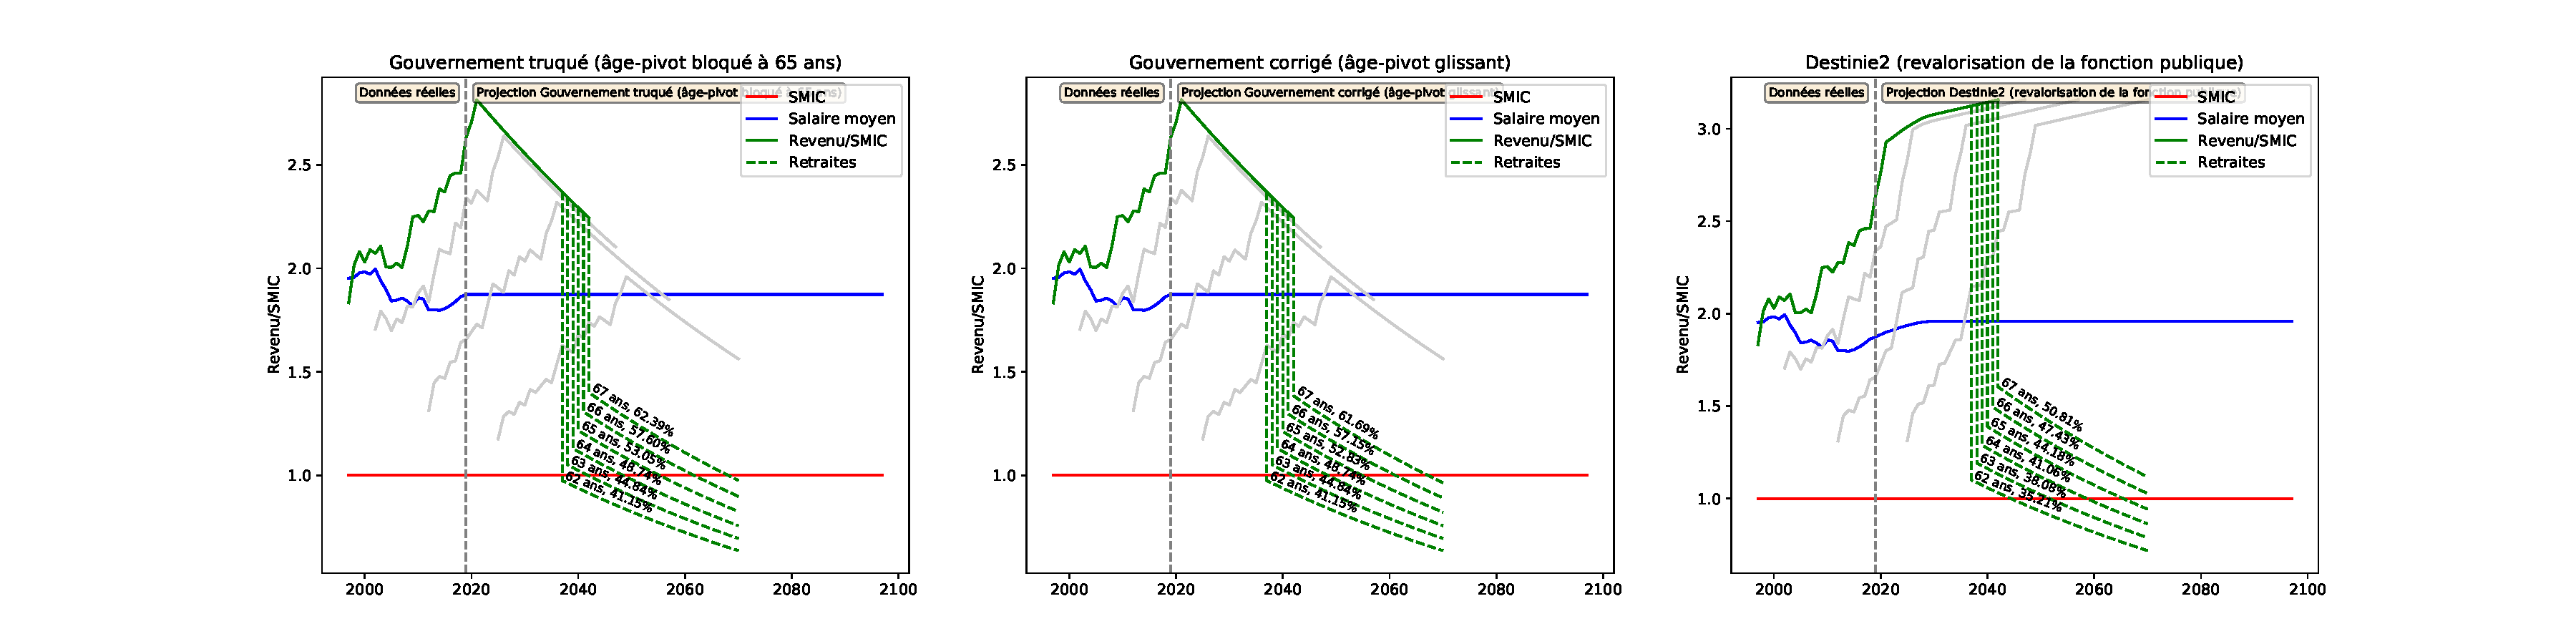
\includegraphics[width=0.9\textwidth]{fig/ProfAgrege_1975_22_dest_retraite.pdf}\end{center} \label{fig/ProfAgrege_1975_22_dest_retraite.pdf} 

\newpage 
 
\subsection{Génération 1980 (début en 2002)} 

\paragraph{Retraites possibles et ratios Revenu/SMIC à 70, 75, 80, 85, 90 ans avec le modèle \emph{Gouvernement truqué (âge-pivot bloqué à 65 ans)}}  
 
{ \scriptsize \begin{center} 
\begin{tabular}[htb]{|c|c||c|c||c|c||c||c|c|c|c|c|c|} 
\hline 
 Retraite en &  Âge &  Âge pivot &  Décote/Surcote &  Retraite (\euro{} 2019) &  Tx Rempl(\%) &  SMIC (\euro{} 2019) &  Retraite/SMIC &  Rev70/SMIC &  Rev75/SMIC &  Rev80/SMIC &  Rev85/SMIC &  Rev90/SMIC \\ 
\hline \hline 
 2042 &  62 &  65 ans 0 mois &  -15.00\% &  2115.47 &  {\bf 41.68} &  2285.97 &  {\bf {\color{red} 0.93}} &  {\bf {\color{red} 0.83}} &  {\bf {\color{red} 0.78}} &  {\bf {\color{red} 0.73}} &  {\bf {\color{red} 0.69}} &  {\bf {\color{red} 0.64}} \\ 
\hline 
 2043 &  63 &  65 ans 0 mois &  -10.00\% &  2329.30 &  {\bf 45.80} &  2315.68 &  {\bf 1.01} &  {\bf {\color{red} 0.92}} &  {\bf {\color{red} 0.86}} &  {\bf {\color{red} 0.81}} &  {\bf {\color{red} 0.76}} &  {\bf {\color{red} 0.71}} \\ 
\hline 
 2044 &  64 &  65 ans 0 mois &  -5.00\% &  2556.18 &  {\bf 50.15} &  2345.79 &  {\bf 1.09} &  {\bf 1.01} &  {\bf {\color{red} 0.95}} &  {\bf {\color{red} 0.89}} &  {\bf {\color{red} 0.83}} &  {\bf {\color{red} 0.78}} \\ 
\hline 
 2045 &  65 &  65 ans 0 mois &  0.00\% &  2796.78 &  {\bf 54.76} &  2376.28 &  {\bf 1.18} &  {\bf 1.10} &  {\bf 1.03} &  {\bf {\color{red} 0.97}} &  {\bf {\color{red} 0.91}} &  {\bf {\color{red} 0.85}} \\ 
\hline 
 2046 &  66 &  65 ans 0 mois &  5.00\% &  3049.60 &  {\bf 59.58} &  2407.18 &  {\bf 1.27} &  {\bf 1.20} &  {\bf 1.13} &  {\bf 1.06} &  {\bf {\color{red} 0.99}} &  {\bf {\color{red} 0.93}} \\ 
\hline 
 2047 &  67 &  65 ans 0 mois &  10.00\% &  3314.89 &  {\bf 64.63} &  2438.47 &  {\bf 1.36} &  {\bf 1.31} &  {\bf 1.23} &  {\bf 1.15} &  {\bf 1.08} &  {\bf 1.01} \\ 
\hline 
\hline 
\end{tabular} 
\end{center} } 
\paragraph{Retraites possibles et ratios Revenu/SMIC à 70, 75, 80, 85, 90 ans avec le modèle \emph{Gouvernement corrigé (âge-pivot glissant)}}  
 
{ \scriptsize \begin{center} 
\begin{tabular}[htb]{|c|c||c|c||c|c||c||c|c|c|c|c|c|} 
\hline 
 Retraite en &  Âge &  Âge pivot &  Décote/Surcote &  Retraite (\euro{} 2019) &  Tx Rempl(\%) &  SMIC (\euro{} 2019) &  Retraite/SMIC &  Rev70/SMIC &  Rev75/SMIC &  Rev80/SMIC &  Rev85/SMIC &  Rev90/SMIC \\ 
\hline \hline 
 2042 &  62 &  65 ans 3 mois &  -16.25\% &  2084.36 &  {\bf 41.07} &  2285.97 &  {\bf {\color{red} 0.91}} &  {\bf {\color{red} 0.82}} &  {\bf {\color{red} 0.77}} &  {\bf {\color{red} 0.72}} &  {\bf {\color{red} 0.68}} &  {\bf {\color{red} 0.64}} \\ 
\hline 
 2043 &  63 &  65 ans 4 mois &  -11.67\% &  2286.17 &  {\bf 44.95} &  2315.68 &  {\bf {\color{red} 0.99}} &  {\bf {\color{red} 0.90}} &  {\bf {\color{red} 0.85}} &  {\bf {\color{red} 0.79}} &  {\bf {\color{red} 0.74}} &  {\bf {\color{red} 0.70}} \\ 
\hline 
 2044 &  64 &  65 ans 5 mois &  -7.08\% &  2500.12 &  {\bf 49.05} &  2345.79 &  {\bf 1.07} &  {\bf {\color{red} 0.99}} &  {\bf {\color{red} 0.92}} &  {\bf {\color{red} 0.87}} &  {\bf {\color{red} 0.81}} &  {\bf {\color{red} 0.76}} \\ 
\hline 
 2045 &  65 &  65 ans 6 mois &  -2.50\% &  2726.86 &  {\bf 53.39} &  2376.28 &  {\bf 1.15} &  {\bf 1.08} &  {\bf 1.01} &  {\bf {\color{red} 0.95}} &  {\bf {\color{red} 0.89}} &  {\bf {\color{red} 0.83}} \\ 
\hline 
 2046 &  66 &  65 ans 7 mois &  2.08\% &  2964.89 &  {\bf 57.93} &  2407.18 &  {\bf 1.23} &  {\bf 1.17} &  {\bf 1.10} &  {\bf 1.03} &  {\bf {\color{red} 0.96}} &  {\bf {\color{red} 0.90}} \\ 
\hline 
 2047 &  67 &  65 ans 8 mois &  6.67\% &  3214.44 &  {\bf 62.67} &  2438.47 &  {\bf 1.32} &  {\bf 1.27} &  {\bf 1.19} &  {\bf 1.11} &  {\bf 1.04} &  {\bf {\color{red} 0.98}} \\ 
\hline 
\hline 
\end{tabular} 
\end{center} } 
\paragraph{Retraites possibles et ratios Revenu/SMIC à 70, 75, 80, 85, 90 ans avec le modèle \emph{Destinie2 (revalorisation de la fonction publique)}}  
 
{ \scriptsize \begin{center} 
\begin{tabular}[htb]{|c|c||c|c||c|c||c||c|c|c|c|c|c|} 
\hline 
 Retraite en &  Âge &  Âge pivot &  Décote/Surcote &  Retraite (\euro{} 2019) &  Tx Rempl(\%) &  SMIC (\euro{} 2019) &  Retraite/SMIC &  Rev70/SMIC &  Rev75/SMIC &  Rev80/SMIC &  Rev85/SMIC &  Rev90/SMIC \\ 
\hline \hline 
 2042 &  62 &  65 ans 3 mois &  -16.25\% &  2399.13 &  {\bf 35.51} &  2149.23 &  {\bf 1.12} &  {\bf 1.01} &  {\bf {\color{red} 0.94}} &  {\bf {\color{red} 0.88}} &  {\bf {\color{red} 0.83}} &  {\bf {\color{red} 0.78}} \\ 
\hline 
 2043 &  63 &  65 ans 4 mois &  -11.67\% &  2643.57 &  {\bf 38.63} &  2177.17 &  {\bf 1.21} &  {\bf 1.11} &  {\bf 1.04} &  {\bf {\color{red} 0.97}} &  {\bf {\color{red} 0.91}} &  {\bf {\color{red} 0.86}} \\ 
\hline 
 2044 &  64 &  65 ans 5 mois &  -7.08\% &  2904.41 &  {\bf 41.90} &  2205.48 &  {\bf 1.32} &  {\bf 1.22} &  {\bf 1.14} &  {\bf 1.07} &  {\bf 1.00} &  {\bf {\color{red} 0.94}} \\ 
\hline 
 2045 &  65 &  65 ans 6 mois &  -2.50\% &  3182.61 &  {\bf 45.32} &  2234.15 &  {\bf 1.42} &  {\bf 1.34} &  {\bf 1.25} &  {\bf 1.17} &  {\bf 1.10} &  {\bf 1.03} \\ 
\hline 
 2046 &  66 &  65 ans 7 mois &  2.08\% &  3476.62 &  {\bf 48.87} &  2263.19 &  {\bf 1.54} &  {\bf 1.46} &  {\bf 1.37} &  {\bf 1.28} &  {\bf 1.20} &  {\bf 1.13} \\ 
\hline 
 2047 &  67 &  65 ans 8 mois &  6.67\% &  3786.93 &  {\bf 52.55} &  2292.61 &  {\bf 1.65} &  {\bf 1.59} &  {\bf 1.49} &  {\bf 1.40} &  {\bf 1.31} &  {\bf 1.23} \\ 
\hline 
\hline 
\end{tabular} 
\end{center} } 

 \begin{center}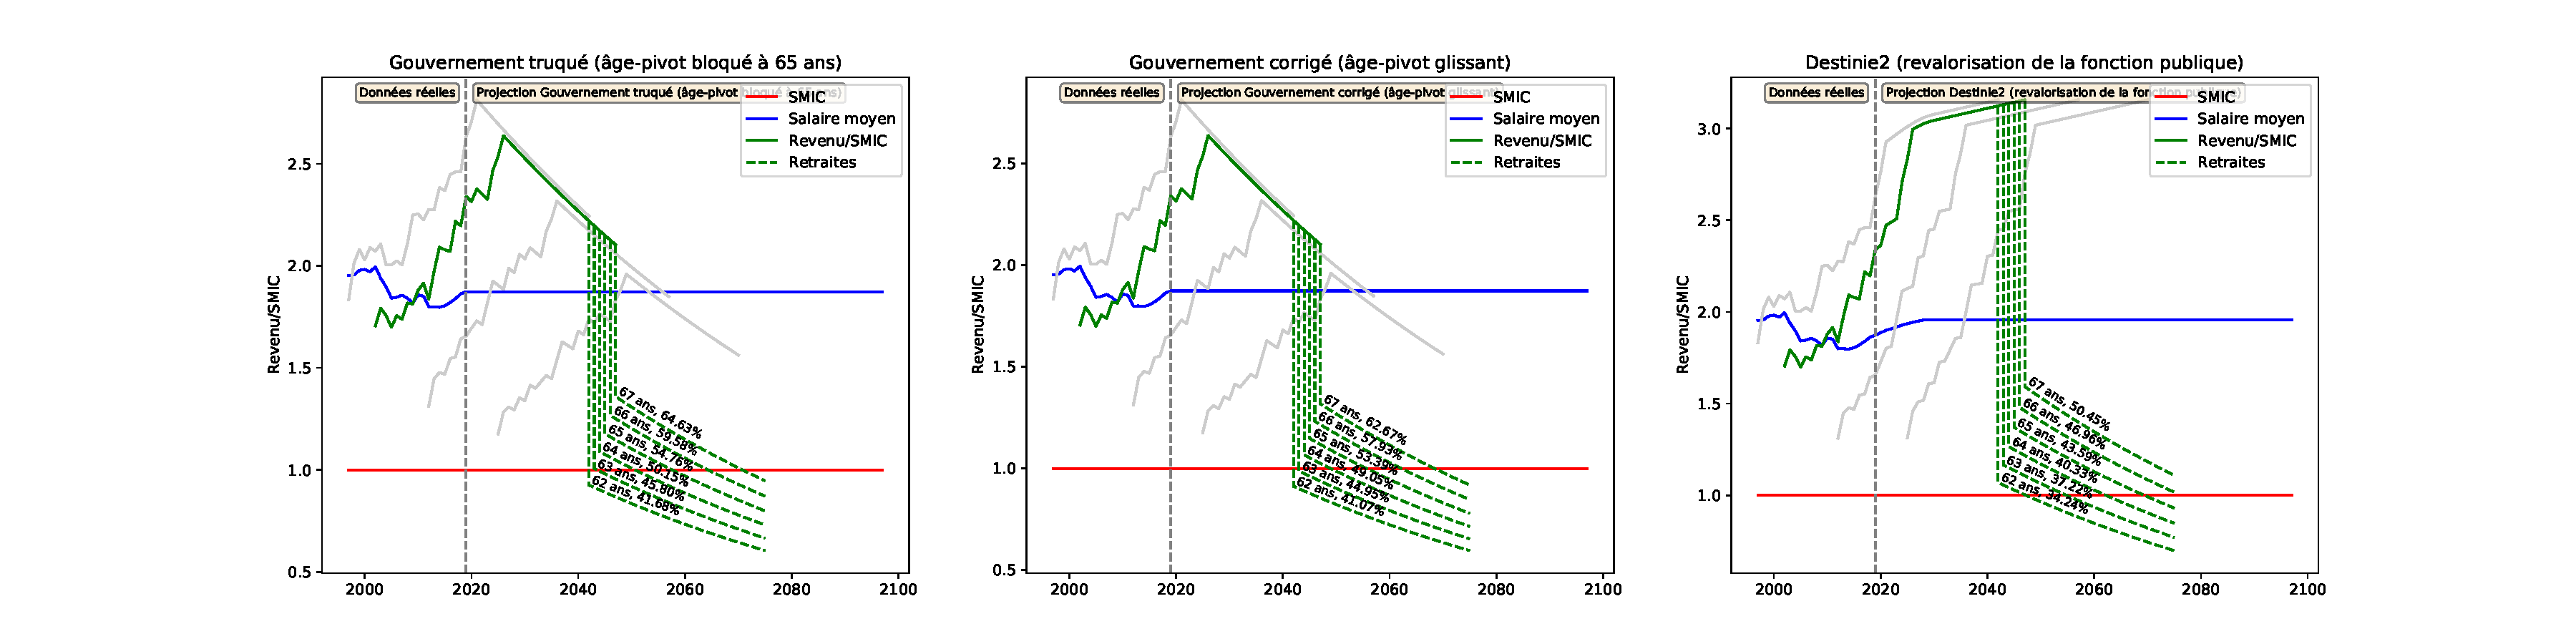
\includegraphics[width=0.9\textwidth]{fig/ProfAgrege_1980_22_dest_retraite.pdf}\end{center} \label{fig/ProfAgrege_1980_22_dest_retraite.pdf} 

\newpage 
 
\subsection{Génération 1990 (début en 2012)} 

\paragraph{Retraites possibles et ratios Revenu/SMIC à 70, 75, 80, 85, 90 ans avec le modèle \emph{Gouvernement truqué (âge-pivot bloqué à 65 ans)}}  
 
{ \scriptsize \begin{center} 
\begin{tabular}[htb]{|c|c||c|c||c|c||c||c|c|c|c|c|c|} 
\hline 
 Retraite en &  Âge &  Âge pivot &  Décote/Surcote &  Retraite (\euro{} 2019) &  Tx Rempl(\%) &  SMIC (\euro{} 2019) &  Retraite/SMIC &  Rev70/SMIC &  Rev75/SMIC &  Rev80/SMIC &  Rev85/SMIC &  Rev90/SMIC \\ 
\hline \hline 
 2052 &  62 &  65 ans 0 mois &  -15.00\% &  2269.42 &  {\bf 44.71} &  2601.14 &  {\bf {\color{red} 0.87}} &  {\bf {\color{red} 0.79}} &  {\bf {\color{red} 0.74}} &  {\bf {\color{red} 0.69}} &  {\bf {\color{red} 0.65}} &  {\bf {\color{red} 0.61}} \\ 
\hline 
 2053 &  63 &  65 ans 0 mois &  -10.00\% &  2497.87 &  {\bf 49.11} &  2634.96 &  {\bf {\color{red} 0.95}} &  {\bf {\color{red} 0.87}} &  {\bf {\color{red} 0.81}} &  {\bf {\color{red} 0.76}} &  {\bf {\color{red} 0.71}} &  {\bf {\color{red} 0.67}} \\ 
\hline 
 2054 &  64 &  65 ans 0 mois &  -5.00\% &  2738.31 &  {\bf 53.73} &  2669.21 &  {\bf 1.03} &  {\bf {\color{red} 0.95}} &  {\bf {\color{red} 0.89}} &  {\bf {\color{red} 0.83}} &  {\bf {\color{red} 0.78}} &  {\bf {\color{red} 0.73}} \\ 
\hline 
 2055 &  65 &  65 ans 0 mois &  0.00\% &  2991.00 &  {\bf 58.56} &  2703.91 &  {\bf 1.11} &  {\bf 1.04} &  {\bf {\color{red} 0.97}} &  {\bf {\color{red} 0.91}} &  {\bf {\color{red} 0.85}} &  {\bf {\color{red} 0.80}} \\ 
\hline 
 2056 &  66 &  65 ans 0 mois &  5.00\% &  3256.18 &  {\bf 63.62} &  2739.06 &  {\bf 1.19} &  {\bf 1.13} &  {\bf 1.06} &  {\bf {\color{red} 0.99}} &  {\bf {\color{red} 0.93}} &  {\bf {\color{red} 0.87}} \\ 
\hline 
 2057 &  67 &  65 ans 0 mois &  10.00\% &  3534.12 &  {\bf 68.90} &  2774.67 &  {\bf 1.27} &  {\bf 1.23} &  {\bf 1.15} &  {\bf 1.08} &  {\bf 1.01} &  {\bf {\color{red} 0.95}} \\ 
\hline 
\hline 
\end{tabular} 
\end{center} } 
\paragraph{Retraites possibles et ratios Revenu/SMIC à 70, 75, 80, 85, 90 ans avec le modèle \emph{Gouvernement corrigé (âge-pivot glissant)}}  
 
{ \scriptsize \begin{center} 
\begin{tabular}[htb]{|c|c||c|c||c|c||c||c|c|c|c|c|c|} 
\hline 
 Retraite en &  Âge &  Âge pivot &  Décote/Surcote &  Retraite (\euro{} 2019) &  Tx Rempl(\%) &  SMIC (\euro{} 2019) &  Retraite/SMIC &  Rev70/SMIC &  Rev75/SMIC &  Rev80/SMIC &  Rev85/SMIC &  Rev90/SMIC \\ 
\hline \hline 
 2052 &  62 &  66 ans 1 mois &  -20.42\% &  2124.80 &  {\bf 41.86} &  2601.14 &  {\bf {\color{red} 0.82}} &  {\bf {\color{red} 0.74}} &  {\bf {\color{red} 0.69}} &  {\bf {\color{red} 0.65}} &  {\bf {\color{red} 0.61}} &  {\bf {\color{red} 0.57}} \\ 
\hline 
 2053 &  63 &  66 ans 2 mois &  -15.83\% &  2335.97 &  {\bf 45.93} &  2634.96 &  {\bf {\color{red} 0.89}} &  {\bf {\color{red} 0.81}} &  {\bf {\color{red} 0.76}} &  {\bf {\color{red} 0.71}} &  {\bf {\color{red} 0.67}} &  {\bf {\color{red} 0.63}} \\ 
\hline 
 2054 &  64 &  66 ans 3 mois &  -11.25\% &  2558.16 &  {\bf 50.19} &  2669.21 &  {\bf {\color{red} 0.96}} &  {\bf {\color{red} 0.89}} &  {\bf {\color{red} 0.83}} &  {\bf {\color{red} 0.78}} &  {\bf {\color{red} 0.73}} &  {\bf {\color{red} 0.69}} \\ 
\hline 
 2055 &  65 &  66 ans 4 mois &  -6.67\% &  2791.60 &  {\bf 54.66} &  2703.91 &  {\bf 1.03} &  {\bf {\color{red} 0.97}} &  {\bf {\color{red} 0.91}} &  {\bf {\color{red} 0.85}} &  {\bf {\color{red} 0.80}} &  {\bf {\color{red} 0.75}} \\ 
\hline 
 2056 &  66 &  66 ans 5 mois &  -2.08\% &  3036.52 &  {\bf 59.33} &  2739.06 &  {\bf 1.11} &  {\bf 1.05} &  {\bf {\color{red} 0.99}} &  {\bf {\color{red} 0.93}} &  {\bf {\color{red} 0.87}} &  {\bf {\color{red} 0.81}} \\ 
\hline 
 2057 &  67 &  66 ans 6 mois &  2.50\% &  3293.15 &  {\bf 64.21} &  2774.67 &  {\bf 1.19} &  {\bf 1.14} &  {\bf 1.07} &  {\bf 1.00} &  {\bf {\color{red} 0.94}} &  {\bf {\color{red} 0.88}} \\ 
\hline 
\hline 
\end{tabular} 
\end{center} } 
\paragraph{Retraites possibles et ratios Revenu/SMIC à 70, 75, 80, 85, 90 ans avec le modèle \emph{Destinie2 (revalorisation de la fonction publique)}}  
 
{ \scriptsize \begin{center} 
\begin{tabular}[htb]{|c|c||c|c||c|c||c||c|c|c|c|c|c|} 
\hline 
 Retraite en &  Âge &  Âge pivot &  Décote/Surcote &  Retraite (\euro{} 2019) &  Tx Rempl(\%) &  SMIC (\euro{} 2019) &  Retraite/SMIC &  Rev70/SMIC &  Rev75/SMIC &  Rev80/SMIC &  Rev85/SMIC &  Rev90/SMIC \\ 
\hline \hline 
 2052 &  62 &  66 ans 1 mois &  -20.42\% &  2694.08 &  {\bf 35.05} &  2445.56 &  {\bf 1.10} &  {\bf {\color{red} 0.99}} &  {\bf {\color{red} 0.93}} &  {\bf {\color{red} 0.87}} &  {\bf {\color{red} 0.82}} &  {\bf {\color{red} 0.77}} \\ 
\hline 
 2053 &  63 &  66 ans 2 mois &  -15.83\% &  2977.50 &  {\bf 38.24} &  2477.35 &  {\bf 1.20} &  {\bf 1.10} &  {\bf 1.03} &  {\bf {\color{red} 0.96}} &  {\bf {\color{red} 0.90}} &  {\bf {\color{red} 0.85}} \\ 
\hline 
 2054 &  64 &  66 ans 3 mois &  -11.25\% &  3277.91 &  {\bf 41.55} &  2509.56 &  {\bf 1.31} &  {\bf 1.21} &  {\bf 1.13} &  {\bf 1.06} &  {\bf {\color{red} 1.00}} &  {\bf {\color{red} 0.93}} \\ 
\hline 
 2055 &  65 &  66 ans 4 mois &  -6.67\% &  3595.82 &  {\bf 45.00} &  2542.18 &  {\bf 1.41} &  {\bf 1.33} &  {\bf 1.24} &  {\bf 1.17} &  {\bf 1.09} &  {\bf 1.02} \\ 
\hline 
 2056 &  66 &  66 ans 5 mois &  -2.08\% &  3931.76 &  {\bf 48.57} &  2575.23 &  {\bf 1.53} &  {\bf 1.45} &  {\bf 1.36} &  {\bf 1.27} &  {\bf 1.19} &  {\bf 1.12} \\ 
\hline 
 2057 &  67 &  66 ans 6 mois &  2.50\% &  4286.30 &  {\bf 52.27} &  2608.71 &  {\bf 1.64} &  {\bf 1.58} &  {\bf 1.48} &  {\bf 1.39} &  {\bf 1.30} &  {\bf 1.22} \\ 
\hline 
\hline 
\end{tabular} 
\end{center} } 

 \begin{center}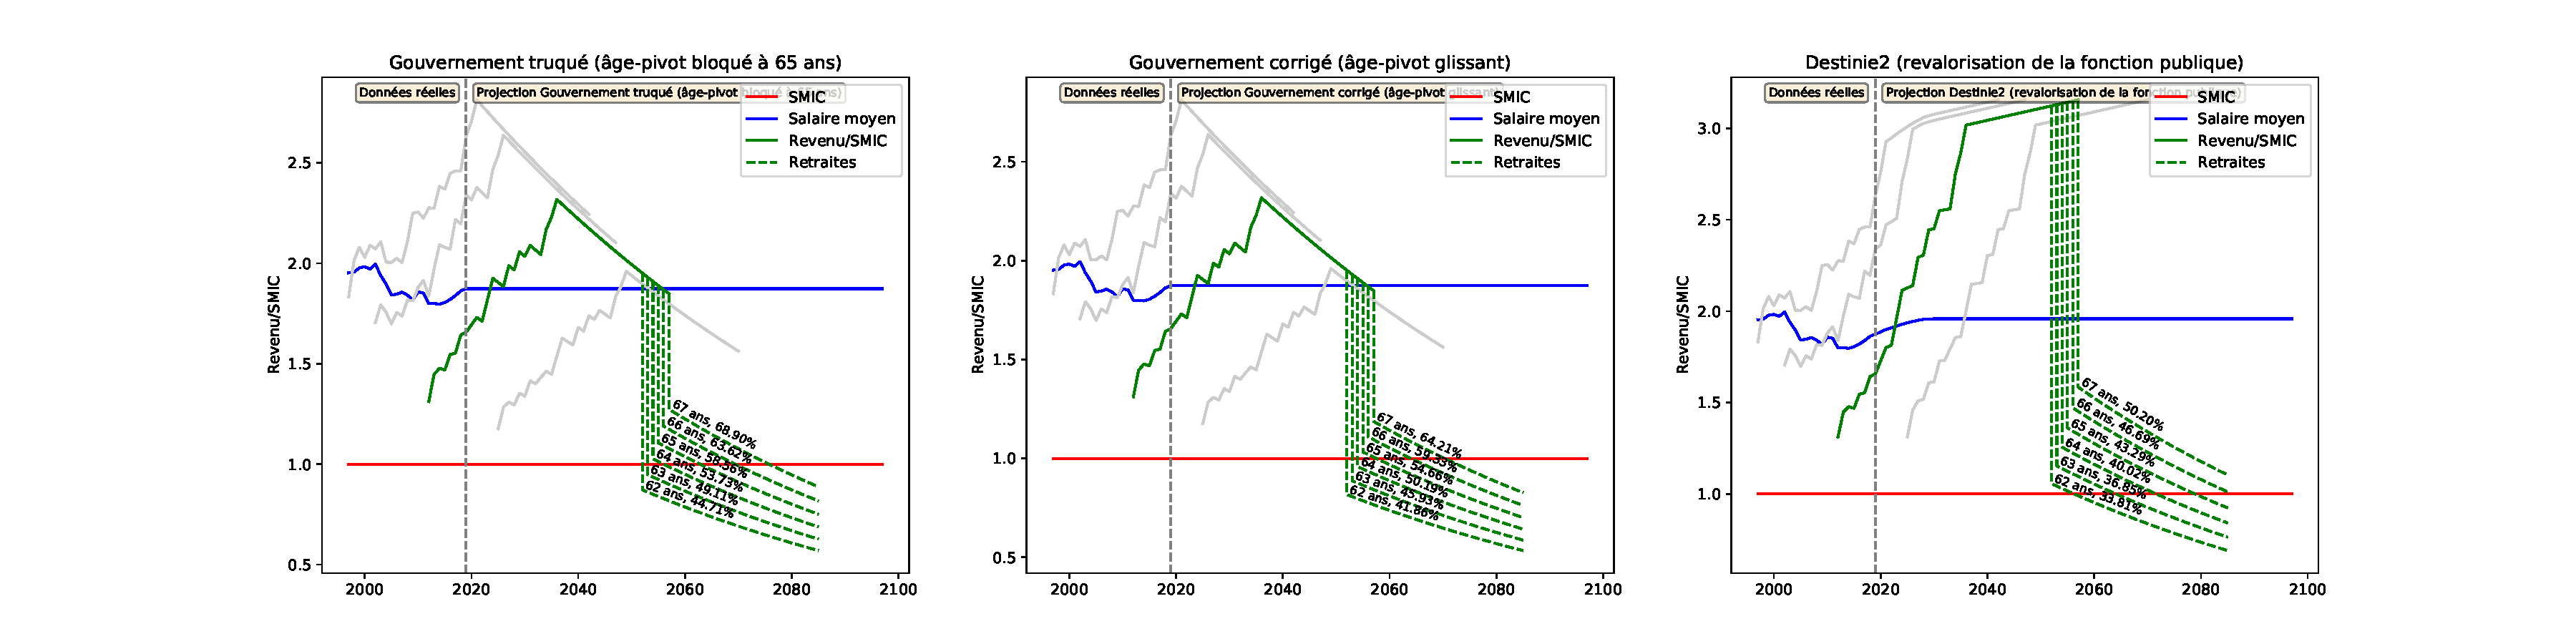
\includegraphics[width=0.9\textwidth]{fig/ProfAgrege_1990_22_dest_retraite.pdf}\end{center} \label{fig/ProfAgrege_1990_22_dest_retraite.pdf} 

\newpage 
 
\subsection{Génération 2003 (début en 2025)} 

\paragraph{Retraites possibles et ratios Revenu/SMIC à 70, 75, 80, 85, 90 ans avec le modèle \emph{Gouvernement truqué (âge-pivot bloqué à 65 ans)}}  
 
{ \scriptsize \begin{center} 
\begin{tabular}[htb]{|c|c||c|c||c|c||c||c|c|c|c|c|c|} 
\hline 
 Retraite en &  Âge &  Âge pivot &  Décote/Surcote &  Retraite (\euro{} 2019) &  Tx Rempl(\%) &  SMIC (\euro{} 2019) &  Retraite/SMIC &  Rev70/SMIC &  Rev75/SMIC &  Rev80/SMIC &  Rev85/SMIC &  Rev90/SMIC \\ 
\hline \hline 
 2065 &  62 &  65 ans 0 mois &  -15.00\% &  2415.39 &  {\bf 47.59} &  3076.71 &  {\bf {\color{red} 0.79}} &  {\bf {\color{red} 0.71}} &  {\bf {\color{red} 0.66}} &  {\bf {\color{red} 0.62}} &  {\bf {\color{red} 0.58}} &  {\bf {\color{red} 0.55}} \\ 
\hline 
 2066 &  63 &  65 ans 0 mois &  -10.00\% &  2654.44 &  {\bf 52.19} &  3116.71 &  {\bf {\color{red} 0.85}} &  {\bf {\color{red} 0.78}} &  {\bf {\color{red} 0.73}} &  {\bf {\color{red} 0.68}} &  {\bf {\color{red} 0.64}} &  {\bf {\color{red} 0.60}} \\ 
\hline 
 2067 &  64 &  65 ans 0 mois &  -5.00\% &  2905.73 &  {\bf 57.01} &  3157.23 &  {\bf {\color{red} 0.92}} &  {\bf {\color{red} 0.85}} &  {\bf {\color{red} 0.80}} &  {\bf {\color{red} 0.75}} &  {\bf {\color{red} 0.70}} &  {\bf {\color{red} 0.66}} \\ 
\hline 
 2068 &  65 &  65 ans 0 mois &  0.00\% &  3169.52 &  {\bf 62.06} &  3198.27 &  {\bf {\color{red} 0.99}} &  {\bf {\color{red} 0.93}} &  {\bf {\color{red} 0.87}} &  {\bf {\color{red} 0.82}} &  {\bf {\color{red} 0.77}} &  {\bf {\color{red} 0.72}} \\ 
\hline 
 2069 &  66 &  65 ans 0 mois &  5.00\% &  3446.06 &  {\bf 67.33} &  3239.85 &  {\bf 1.06} &  {\bf 1.01} &  {\bf {\color{red} 0.95}} &  {\bf {\color{red} 0.89}} &  {\bf {\color{red} 0.83}} &  {\bf {\color{red} 0.78}} \\ 
\hline 
 2070 &  67 &  65 ans 0 mois &  10.00\% &  3735.62 &  {\bf 72.83} &  3281.97 &  {\bf 1.14} &  {\bf 1.09} &  {\bf 1.03} &  {\bf {\color{red} 0.96}} &  {\bf {\color{red} 0.90}} &  {\bf {\color{red} 0.85}} \\ 
\hline 
\hline 
\end{tabular} 
\end{center} } 
\paragraph{Retraites possibles et ratios Revenu/SMIC à 70, 75, 80, 85, 90 ans avec le modèle \emph{Gouvernement corrigé (âge-pivot glissant)}}  
 
{ \scriptsize \begin{center} 
\begin{tabular}[htb]{|c|c||c|c||c|c||c||c|c|c|c|c|c|} 
\hline 
 Retraite en &  Âge &  Âge pivot &  Décote/Surcote &  Retraite (\euro{} 2019) &  Tx Rempl(\%) &  SMIC (\euro{} 2019) &  Retraite/SMIC &  Rev70/SMIC &  Rev75/SMIC &  Rev80/SMIC &  Rev85/SMIC &  Rev90/SMIC \\ 
\hline \hline 
 2065 &  62 &  67 ans 2 mois &  -25.83\% &  2107.55 &  {\bf 41.52} &  3076.71 &  {\bf {\color{red} 0.68}} &  {\bf {\color{red} 0.62}} &  {\bf {\color{red} 0.58}} &  {\bf {\color{red} 0.54}} &  {\bf {\color{red} 0.51}} &  {\bf {\color{red} 0.48}} \\ 
\hline 
 2066 &  63 &  67 ans 3 mois &  -21.25\% &  2322.63 &  {\bf 45.67} &  3116.71 &  {\bf {\color{red} 0.75}} &  {\bf {\color{red} 0.68}} &  {\bf {\color{red} 0.64}} &  {\bf {\color{red} 0.60}} &  {\bf {\color{red} 0.56}} &  {\bf {\color{red} 0.53}} \\ 
\hline 
 2067 &  64 &  67 ans 4 mois &  -16.67\% &  2548.88 &  {\bf 50.01} &  3157.23 &  {\bf {\color{red} 0.81}} &  {\bf {\color{red} 0.75}} &  {\bf {\color{red} 0.70}} &  {\bf {\color{red} 0.66}} &  {\bf {\color{red} 0.62}} &  {\bf {\color{red} 0.58}} \\ 
\hline 
 2068 &  65 &  67 ans 5 mois &  -12.08\% &  2786.53 &  {\bf 54.56} &  3198.27 &  {\bf {\color{red} 0.87}} &  {\bf {\color{red} 0.82}} &  {\bf {\color{red} 0.77}} &  {\bf {\color{red} 0.72}} &  {\bf {\color{red} 0.67}} &  {\bf {\color{red} 0.63}} \\ 
\hline 
 2069 &  66 &  67 ans 6 mois &  -7.50\% &  3035.82 &  {\bf 59.31} &  3239.85 &  {\bf {\color{red} 0.94}} &  {\bf {\color{red} 0.89}} &  {\bf {\color{red} 0.83}} &  {\bf {\color{red} 0.78}} &  {\bf {\color{red} 0.73}} &  {\bf {\color{red} 0.69}} \\ 
\hline 
 2070 &  67 &  67 ans 7 mois &  -2.92\% &  3296.97 &  {\bf 64.28} &  3281.97 &  {\bf 1.00} &  {\bf {\color{red} 0.97}} &  {\bf {\color{red} 0.91}} &  {\bf {\color{red} 0.85}} &  {\bf {\color{red} 0.80}} &  {\bf {\color{red} 0.75}} \\ 
\hline 
\hline 
\end{tabular} 
\end{center} } 
\paragraph{Retraites possibles et ratios Revenu/SMIC à 70, 75, 80, 85, 90 ans avec le modèle \emph{Destinie2 (revalorisation de la fonction publique)}}  
 
{ \scriptsize \begin{center} 
\begin{tabular}[htb]{|c|c||c|c||c|c||c||c|c|c|c|c|c|} 
\hline 
 Retraite en &  Âge &  Âge pivot &  Décote/Surcote &  Retraite (\euro{} 2019) &  Tx Rempl(\%) &  SMIC (\euro{} 2019) &  Retraite/SMIC &  Rev70/SMIC &  Rev75/SMIC &  Rev80/SMIC &  Rev85/SMIC &  Rev90/SMIC \\ 
\hline \hline 
 2065 &  62 &  67 ans 2 mois &  -25.83\% &  3115.87 &  {\bf 34.27} &  2892.68 &  {\bf 1.08} &  {\bf {\color{red} 0.97}} &  {\bf {\color{red} 0.91}} &  {\bf {\color{red} 0.85}} &  {\bf {\color{red} 0.80}} &  {\bf {\color{red} 0.75}} \\ 
\hline 
 2066 &  63 &  67 ans 3 mois &  -21.25\% &  3452.40 &  {\bf 37.48} &  2930.29 &  {\bf 1.18} &  {\bf 1.08} &  {\bf 1.01} &  {\bf {\color{red} 0.95}} &  {\bf {\color{red} 0.89}} &  {\bf {\color{red} 0.83}} \\ 
\hline 
 2067 &  64 &  67 ans 4 mois &  -16.67\% &  3809.05 &  {\bf 40.82} &  2968.38 &  {\bf 1.28} &  {\bf 1.19} &  {\bf 1.11} &  {\bf 1.04} &  {\bf {\color{red} 0.98}} &  {\bf {\color{red} 0.92}} \\ 
\hline 
 2068 &  65 &  67 ans 5 mois &  -12.08\% &  4186.46 &  {\bf 44.29} &  3006.97 &  {\bf 1.39} &  {\bf 1.31} &  {\bf 1.22} &  {\bf 1.15} &  {\bf 1.08} &  {\bf 1.01} \\ 
\hline 
 2069 &  66 &  67 ans 6 mois &  -7.50\% &  4585.25 &  {\bf 47.89} &  3046.06 &  {\bf 1.51} &  {\bf 1.43} &  {\bf 1.34} &  {\bf 1.26} &  {\bf 1.18} &  {\bf 1.10} \\ 
\hline 
 2070 &  67 &  67 ans 7 mois &  -2.92\% &  5006.08 &  {\bf 51.61} &  3085.66 &  {\bf 1.62} &  {\bf 1.56} &  {\bf 1.46} &  {\bf 1.37} &  {\bf 1.29} &  {\bf 1.21} \\ 
\hline 
\hline 
\end{tabular} 
\end{center} } 

 \begin{center}\includegraphics[width=0.9\textwidth]{fig/ProfAgrege_2003_22_dest_retraite.pdf}\end{center} \label{fig/ProfAgrege_2003_22_dest_retraite.pdf} 

\newpage 
 
\chapter{BIATSS (CN puis CS)} 

\begin{minipage}{0.55\linewidth}\includegraphics[width=0.7\textwidth]{fig/grille_BIATSS.pdf}\end{minipage} 
\begin{minipage}{0.3\linewidth} 
 \begin{center} 

\begin{tabular}[htb]{|c|c|} 
\hline 
 Indice majoré &  Durée (années) \\ 
\hline \hline 
 343 &  2.00 \\ 
\hline 
 349 &  2.00 \\ 
\hline 
 355 &  2.00 \\ 
\hline 
 361 &  2.00 \\ 
\hline 
 369 &  2.00 \\ 
\hline 
 381 &  2.00 \\ 
\hline 
 396 &  2.00 \\ 
\hline 
 415 &  3.00 \\ 
\hline 
 431 &  3.00 \\ 
\hline 
 441 &  3.00 \\ 
\hline 
 457 &  3.00 \\ 
\hline 
 477 &  4.00 \\ 
\hline 
 503 &  4.00 \\ 
\hline 
 534 &   \\ 
\hline 
\hline 
\end{tabular} 
\end{center} 
 \end{minipage} 


 \addto{\captionsenglish}{ \renewcommand{\mtctitle}{}} \setcounter{minitocdepth}{2} 
 \minitoc \newpage 

\section{Début de carrière à 22 ans} 

\subsection{Génération 1975 (début en 1997)} 

\paragraph{Retraites possibles et ratios Revenu/SMIC à 70, 75, 80, 85, 90 ans avec le modèle \emph{Gouvernement truqué (âge-pivot bloqué à 65 ans)}}  
 
{ \scriptsize \begin{center} 
\begin{tabular}[htb]{|c|c||c|c||c|c||c||c|c|c|c|c|c|} 
\hline 
 Retraite en &  Âge &  Âge pivot &  Décote/Surcote &  Retraite (\euro{} 2019) &  Tx Rempl(\%) &  SMIC (\euro{} 2019) &  Retraite/SMIC &  Rev70/SMIC &  Rev75/SMIC &  Rev80/SMIC &  Rev85/SMIC &  Rev90/SMIC \\ 
\hline \hline 
 2037 &  62 &  64 ans 10 mois &  -14.17\% &  1156.45 &  {\bf 41.32} &  2143.00 &  {\bf {\color{red} 0.54}} &  {\bf {\color{red} 0.49}} &  {\bf {\color{red} 0.46}} &  {\bf {\color{red} 0.43}} &  {\bf {\color{red} 0.40}} &  {\bf {\color{red} 0.38}} \\ 
\hline 
 2038 &  63 &  64 ans 11 mois &  -9.58\% &  1262.78 &  {\bf 45.03} &  2170.86 &  {\bf {\color{red} 0.58}} &  {\bf {\color{red} 0.53}} &  {\bf {\color{red} 0.50}} &  {\bf {\color{red} 0.47}} &  {\bf {\color{red} 0.44}} &  {\bf {\color{red} 0.41}} \\ 
\hline 
 2039 &  64 &  65 ans 0 mois &  -5.00\% &  1375.09 &  {\bf 48.93} &  2199.08 &  {\bf {\color{red} 0.63}} &  {\bf {\color{red} 0.58}} &  {\bf {\color{red} 0.54}} &  {\bf {\color{red} 0.51}} &  {\bf {\color{red} 0.48}} &  {\bf {\color{red} 0.45}} \\ 
\hline 
 2040 &  65 &  65 ans 0 mois &  0.00\% &  1893.52 &  {\bf 67.24} &  2227.67 &  {\bf {\color{red} 0.85}} &  {\bf {\color{red} 0.80}} &  {\bf {\color{red} 0.75}} &  {\bf {\color{red} 0.70}} &  {\bf {\color{red} 0.66}} &  {\bf {\color{red} 0.62}} \\ 
\hline 
 2041 &  66 &  65 ans 0 mois &  5.00\% &  1918.14 &  {\bf 67.97} &  2256.63 &  {\bf {\color{red} 0.85}} &  {\bf {\color{red} 0.81}} &  {\bf {\color{red} 0.76}} &  {\bf {\color{red} 0.71}} &  {\bf {\color{red} 0.67}} &  {\bf {\color{red} 0.62}} \\ 
\hline 
 2042 &  67 &  65 ans 0 mois &  10.00\% &  1943.07 &  {\bf 68.71} &  2285.97 &  {\bf {\color{red} 0.85}} &  {\bf {\color{red} 0.82}} &  {\bf {\color{red} 0.77}} &  {\bf {\color{red} 0.72}} &  {\bf {\color{red} 0.67}} &  {\bf {\color{red} 0.63}} \\ 
\hline 
\hline 
\end{tabular} 
\end{center} } 
\paragraph{Retraites possibles et ratios Revenu/SMIC à 70, 75, 80, 85, 90 ans avec le modèle \emph{Gouvernement corrigé (âge-pivot glissant)}}  
 
{ \scriptsize \begin{center} 
\begin{tabular}[htb]{|c|c||c|c||c|c||c||c|c|c|c|c|c|} 
\hline 
 Retraite en &  Âge &  Âge pivot &  Décote/Surcote &  Retraite (\euro{} 2019) &  Tx Rempl(\%) &  SMIC (\euro{} 2019) &  Retraite/SMIC &  Rev70/SMIC &  Rev75/SMIC &  Rev80/SMIC &  Rev85/SMIC &  Rev90/SMIC \\ 
\hline \hline 
 2037 &  62 &  64 ans 10 mois &  -14.17\% &  1156.45 &  {\bf 41.32} &  2143.00 &  {\bf {\color{red} 0.54}} &  {\bf {\color{red} 0.49}} &  {\bf {\color{red} 0.46}} &  {\bf {\color{red} 0.43}} &  {\bf {\color{red} 0.40}} &  {\bf {\color{red} 0.38}} \\ 
\hline 
 2038 &  63 &  64 ans 11 mois &  -9.58\% &  1262.78 &  {\bf 45.03} &  2170.86 &  {\bf {\color{red} 0.58}} &  {\bf {\color{red} 0.53}} &  {\bf {\color{red} 0.50}} &  {\bf {\color{red} 0.47}} &  {\bf {\color{red} 0.44}} &  {\bf {\color{red} 0.41}} \\ 
\hline 
 2039 &  64 &  65 ans 0 mois &  -5.00\% &  1375.09 &  {\bf 48.93} &  2199.08 &  {\bf {\color{red} 0.63}} &  {\bf {\color{red} 0.58}} &  {\bf {\color{red} 0.54}} &  {\bf {\color{red} 0.51}} &  {\bf {\color{red} 0.48}} &  {\bf {\color{red} 0.45}} \\ 
\hline 
 2040 &  65 &  65 ans 1 mois &  -0.42\% &  1893.52 &  {\bf 67.24} &  2227.67 &  {\bf {\color{red} 0.85}} &  {\bf {\color{red} 0.80}} &  {\bf {\color{red} 0.75}} &  {\bf {\color{red} 0.70}} &  {\bf {\color{red} 0.66}} &  {\bf {\color{red} 0.62}} \\ 
\hline 
 2041 &  66 &  65 ans 2 mois &  4.17\% &  1918.14 &  {\bf 67.97} &  2256.63 &  {\bf {\color{red} 0.85}} &  {\bf {\color{red} 0.81}} &  {\bf {\color{red} 0.76}} &  {\bf {\color{red} 0.71}} &  {\bf {\color{red} 0.67}} &  {\bf {\color{red} 0.62}} \\ 
\hline 
 2042 &  67 &  65 ans 3 mois &  8.75\% &  1943.07 &  {\bf 68.71} &  2285.97 &  {\bf {\color{red} 0.85}} &  {\bf {\color{red} 0.82}} &  {\bf {\color{red} 0.77}} &  {\bf {\color{red} 0.72}} &  {\bf {\color{red} 0.67}} &  {\bf {\color{red} 0.63}} \\ 
\hline 
\hline 
\end{tabular} 
\end{center} } 
\paragraph{Retraites possibles et ratios Revenu/SMIC à 70, 75, 80, 85, 90 ans avec le modèle \emph{Destinie2 (revalorisation de la fonction publique)}}  
 
{ \scriptsize \begin{center} 
\begin{tabular}[htb]{|c|c||c|c||c|c||c||c|c|c|c|c|c|} 
\hline 
 Retraite en &  Âge &  Âge pivot &  Décote/Surcote &  Retraite (\euro{} 2019) &  Tx Rempl(\%) &  SMIC (\euro{} 2019) &  Retraite/SMIC &  Rev70/SMIC &  Rev75/SMIC &  Rev80/SMIC &  Rev85/SMIC &  Rev90/SMIC \\ 
\hline \hline 
 2037 &  62 &  64 ans 10 mois &  -14.17\% &  1283.31 &  {\bf 36.75} &  2014.82 &  {\bf {\color{red} 0.64}} &  {\bf {\color{red} 0.57}} &  {\bf {\color{red} 0.54}} &  {\bf {\color{red} 0.50}} &  {\bf {\color{red} 0.47}} &  {\bf {\color{red} 0.44}} \\ 
\hline 
 2038 &  63 &  64 ans 11 mois &  -9.58\% &  1406.67 &  {\bf 39.76} &  2041.01 &  {\bf {\color{red} 0.69}} &  {\bf {\color{red} 0.63}} &  {\bf {\color{red} 0.59}} &  {\bf {\color{red} 0.55}} &  {\bf {\color{red} 0.52}} &  {\bf {\color{red} 0.49}} \\ 
\hline 
 2039 &  64 &  65 ans 0 mois &  -5.00\% &  1537.76 &  {\bf 42.91} &  2067.55 &  {\bf {\color{red} 0.74}} &  {\bf {\color{red} 0.69}} &  {\bf {\color{red} 0.65}} &  {\bf {\color{red} 0.60}} &  {\bf {\color{red} 0.57}} &  {\bf {\color{red} 0.53}} \\ 
\hline 
 2040 &  65 &  65 ans 1 mois &  -0.42\% &  1780.26 &  {\bf 49.04} &  2094.43 &  {\bf {\color{red} 0.85}} &  {\bf {\color{red} 0.80}} &  {\bf {\color{red} 0.75}} &  {\bf {\color{red} 0.70}} &  {\bf {\color{red} 0.66}} &  {\bf {\color{red} 0.62}} \\ 
\hline 
 2041 &  66 &  65 ans 2 mois &  4.17\% &  1824.95 &  {\bf 49.63} &  2121.65 &  {\bf {\color{red} 0.86}} &  {\bf {\color{red} 0.82}} &  {\bf {\color{red} 0.77}} &  {\bf {\color{red} 0.72}} &  {\bf {\color{red} 0.67}} &  {\bf {\color{red} 0.63}} \\ 
\hline 
 2042 &  67 &  65 ans 3 mois &  8.75\% &  1982.01 &  {\bf 53.21} &  2149.23 &  {\bf {\color{red} 0.92}} &  {\bf {\color{red} 0.89}} &  {\bf {\color{red} 0.83}} &  {\bf {\color{red} 0.78}} &  {\bf {\color{red} 0.73}} &  {\bf {\color{red} 0.69}} \\ 
\hline 
\hline 
\end{tabular} 
\end{center} } 

 \begin{center}\includegraphics[width=0.9\textwidth]{fig/BIATSS_1975_22_dest_retraite.pdf}\end{center} \label{fig/BIATSS_1975_22_dest_retraite.pdf} 

\newpage 
 
\subsection{Génération 1980 (début en 2002)} 

\paragraph{Retraites possibles et ratios Revenu/SMIC à 70, 75, 80, 85, 90 ans avec le modèle \emph{Gouvernement truqué (âge-pivot bloqué à 65 ans)}}  
 
{ \scriptsize \begin{center} 
\begin{tabular}[htb]{|c|c||c|c||c|c||c||c|c|c|c|c|c|} 
\hline 
 Retraite en &  Âge &  Âge pivot &  Décote/Surcote &  Retraite (\euro{} 2019) &  Tx Rempl(\%) &  SMIC (\euro{} 2019) &  Retraite/SMIC &  Rev70/SMIC &  Rev75/SMIC &  Rev80/SMIC &  Rev85/SMIC &  Rev90/SMIC \\ 
\hline \hline 
 2042 &  62 &  65 ans 0 mois &  -15.00\% &  1167.64 &  {\bf 41.72} &  2285.97 &  {\bf {\color{red} 0.51}} &  {\bf {\color{red} 0.46}} &  {\bf {\color{red} 0.43}} &  {\bf {\color{red} 0.40}} &  {\bf {\color{red} 0.38}} &  {\bf {\color{red} 0.36}} \\ 
\hline 
 2043 &  63 &  65 ans 0 mois &  -10.00\% &  1285.62 &  {\bf 45.84} &  2315.68 &  {\bf {\color{red} 0.56}} &  {\bf {\color{red} 0.51}} &  {\bf {\color{red} 0.48}} &  {\bf {\color{red} 0.45}} &  {\bf {\color{red} 0.42}} &  {\bf {\color{red} 0.39}} \\ 
\hline 
 2044 &  64 &  65 ans 0 mois &  -5.00\% &  1410.81 &  {\bf 50.20} &  2345.79 &  {\bf {\color{red} 0.60}} &  {\bf {\color{red} 0.56}} &  {\bf {\color{red} 0.52}} &  {\bf {\color{red} 0.49}} &  {\bf {\color{red} 0.46}} &  {\bf {\color{red} 0.43}} \\ 
\hline 
 2045 &  65 &  65 ans 0 mois &  0.00\% &  2019.84 &  {\bf 71.72} &  2376.28 &  {\bf {\color{red} 0.85}} &  {\bf {\color{red} 0.80}} &  {\bf {\color{red} 0.75}} &  {\bf {\color{red} 0.70}} &  {\bf {\color{red} 0.66}} &  {\bf {\color{red} 0.62}} \\ 
\hline 
 2046 &  66 &  65 ans 0 mois &  5.00\% &  2046.10 &  {\bf 72.50} &  2407.18 &  {\bf {\color{red} 0.85}} &  {\bf {\color{red} 0.81}} &  {\bf {\color{red} 0.76}} &  {\bf {\color{red} 0.71}} &  {\bf {\color{red} 0.67}} &  {\bf {\color{red} 0.62}} \\ 
\hline 
 2047 &  67 &  65 ans 0 mois &  10.00\% &  2072.70 &  {\bf 73.29} &  2438.47 &  {\bf {\color{red} 0.85}} &  {\bf {\color{red} 0.82}} &  {\bf {\color{red} 0.77}} &  {\bf {\color{red} 0.72}} &  {\bf {\color{red} 0.67}} &  {\bf {\color{red} 0.63}} \\ 
\hline 
\hline 
\end{tabular} 
\end{center} } 
\paragraph{Retraites possibles et ratios Revenu/SMIC à 70, 75, 80, 85, 90 ans avec le modèle \emph{Gouvernement corrigé (âge-pivot glissant)}}  
 
{ \scriptsize \begin{center} 
\begin{tabular}[htb]{|c|c||c|c||c|c||c||c|c|c|c|c|c|} 
\hline 
 Retraite en &  Âge &  Âge pivot &  Décote/Surcote &  Retraite (\euro{} 2019) &  Tx Rempl(\%) &  SMIC (\euro{} 2019) &  Retraite/SMIC &  Rev70/SMIC &  Rev75/SMIC &  Rev80/SMIC &  Rev85/SMIC &  Rev90/SMIC \\ 
\hline \hline 
 2042 &  62 &  65 ans 3 mois &  -16.25\% &  1150.47 &  {\bf 41.11} &  2285.97 &  {\bf {\color{red} 0.50}} &  {\bf {\color{red} 0.45}} &  {\bf {\color{red} 0.43}} &  {\bf {\color{red} 0.40}} &  {\bf {\color{red} 0.37}} &  {\bf {\color{red} 0.35}} \\ 
\hline 
 2043 &  63 &  65 ans 4 mois &  -11.67\% &  1261.82 &  {\bf 44.99} &  2315.68 &  {\bf {\color{red} 0.54}} &  {\bf {\color{red} 0.50}} &  {\bf {\color{red} 0.47}} &  {\bf {\color{red} 0.44}} &  {\bf {\color{red} 0.41}} &  {\bf {\color{red} 0.38}} \\ 
\hline 
 2044 &  64 &  65 ans 5 mois &  -7.08\% &  1379.87 &  {\bf 49.10} &  2345.79 &  {\bf {\color{red} 0.59}} &  {\bf {\color{red} 0.54}} &  {\bf {\color{red} 0.51}} &  {\bf {\color{red} 0.48}} &  {\bf {\color{red} 0.45}} &  {\bf {\color{red} 0.42}} \\ 
\hline 
 2045 &  65 &  65 ans 6 mois &  -2.50\% &  2019.84 &  {\bf 71.72} &  2376.28 &  {\bf {\color{red} 0.85}} &  {\bf {\color{red} 0.80}} &  {\bf {\color{red} 0.75}} &  {\bf {\color{red} 0.70}} &  {\bf {\color{red} 0.66}} &  {\bf {\color{red} 0.62}} \\ 
\hline 
 2046 &  66 &  65 ans 7 mois &  2.08\% &  2046.10 &  {\bf 72.50} &  2407.18 &  {\bf {\color{red} 0.85}} &  {\bf {\color{red} 0.81}} &  {\bf {\color{red} 0.76}} &  {\bf {\color{red} 0.71}} &  {\bf {\color{red} 0.67}} &  {\bf {\color{red} 0.62}} \\ 
\hline 
 2047 &  67 &  65 ans 8 mois &  6.67\% &  2072.70 &  {\bf 73.29} &  2438.47 &  {\bf {\color{red} 0.85}} &  {\bf {\color{red} 0.82}} &  {\bf {\color{red} 0.77}} &  {\bf {\color{red} 0.72}} &  {\bf {\color{red} 0.67}} &  {\bf {\color{red} 0.63}} \\ 
\hline 
\hline 
\end{tabular} 
\end{center} } 
\paragraph{Retraites possibles et ratios Revenu/SMIC à 70, 75, 80, 85, 90 ans avec le modèle \emph{Destinie2 (revalorisation de la fonction publique)}}  
 
{ \scriptsize \begin{center} 
\begin{tabular}[htb]{|c|c||c|c||c|c||c||c|c|c|c|c|c|} 
\hline 
 Retraite en &  Âge &  Âge pivot &  Décote/Surcote &  Retraite (\euro{} 2019) &  Tx Rempl(\%) &  SMIC (\euro{} 2019) &  Retraite/SMIC &  Rev70/SMIC &  Rev75/SMIC &  Rev80/SMIC &  Rev85/SMIC &  Rev90/SMIC \\ 
\hline \hline 
 2042 &  62 &  65 ans 3 mois &  -16.25\% &  1322.18 &  {\bf 35.49} &  2149.23 &  {\bf {\color{red} 0.62}} &  {\bf {\color{red} 0.55}} &  {\bf {\color{red} 0.52}} &  {\bf {\color{red} 0.49}} &  {\bf {\color{red} 0.46}} &  {\bf {\color{red} 0.43}} \\ 
\hline 
 2043 &  63 &  65 ans 4 mois &  -11.67\% &  1456.92 &  {\bf 38.61} &  2177.17 &  {\bf {\color{red} 0.67}} &  {\bf {\color{red} 0.61}} &  {\bf {\color{red} 0.57}} &  {\bf {\color{red} 0.54}} &  {\bf {\color{red} 0.50}} &  {\bf {\color{red} 0.47}} \\ 
\hline 
 2044 &  64 &  65 ans 5 mois &  -7.08\% &  1600.69 &  {\bf 41.88} &  2205.48 &  {\bf {\color{red} 0.73}} &  {\bf {\color{red} 0.67}} &  {\bf {\color{red} 0.63}} &  {\bf {\color{red} 0.59}} &  {\bf {\color{red} 0.55}} &  {\bf {\color{red} 0.52}} \\ 
\hline 
 2045 &  65 &  65 ans 6 mois &  -2.50\% &  1899.03 &  {\bf 49.04} &  2234.15 &  {\bf {\color{red} 0.85}} &  {\bf {\color{red} 0.80}} &  {\bf {\color{red} 0.75}} &  {\bf {\color{red} 0.70}} &  {\bf {\color{red} 0.66}} &  {\bf {\color{red} 0.62}} \\ 
\hline 
 2046 &  66 &  65 ans 7 mois &  2.08\% &  1923.71 &  {\bf 49.04} &  2263.19 &  {\bf {\color{red} 0.85}} &  {\bf {\color{red} 0.81}} &  {\bf {\color{red} 0.76}} &  {\bf {\color{red} 0.71}} &  {\bf {\color{red} 0.67}} &  {\bf {\color{red} 0.62}} \\ 
\hline 
 2047 &  67 &  65 ans 8 mois &  6.67\% &  2087.16 &  {\bf 52.53} &  2292.61 &  {\bf {\color{red} 0.91}} &  {\bf {\color{red} 0.88}} &  {\bf {\color{red} 0.82}} &  {\bf {\color{red} 0.77}} &  {\bf {\color{red} 0.72}} &  {\bf {\color{red} 0.68}} \\ 
\hline 
\hline 
\end{tabular} 
\end{center} } 

 \begin{center}\includegraphics[width=0.9\textwidth]{fig/BIATSS_1980_22_dest_retraite.pdf}\end{center} \label{fig/BIATSS_1980_22_dest_retraite.pdf} 

\newpage 
 
\subsection{Génération 1990 (début en 2012)} 

\paragraph{Retraites possibles et ratios Revenu/SMIC à 70, 75, 80, 85, 90 ans avec le modèle \emph{Gouvernement truqué (âge-pivot bloqué à 65 ans)}}  
 
{ \scriptsize \begin{center} 
\begin{tabular}[htb]{|c|c||c|c||c|c||c||c|c|c|c|c|c|} 
\hline 
 Retraite en &  Âge &  Âge pivot &  Décote/Surcote &  Retraite (\euro{} 2019) &  Tx Rempl(\%) &  SMIC (\euro{} 2019) &  Retraite/SMIC &  Rev70/SMIC &  Rev75/SMIC &  Rev80/SMIC &  Rev85/SMIC &  Rev90/SMIC \\ 
\hline \hline 
 2052 &  62 &  65 ans 0 mois &  -15.00\% &  1251.06 &  {\bf 44.70} &  2601.14 &  {\bf {\color{red} 0.48}} &  {\bf {\color{red} 0.43}} &  {\bf {\color{red} 0.41}} &  {\bf {\color{red} 0.38}} &  {\bf {\color{red} 0.36}} &  {\bf {\color{red} 0.34}} \\ 
\hline 
 2053 &  63 &  65 ans 0 mois &  -10.00\% &  1377.00 &  {\bf 49.10} &  2634.96 &  {\bf {\color{red} 0.52}} &  {\bf {\color{red} 0.48}} &  {\bf {\color{red} 0.45}} &  {\bf {\color{red} 0.42}} &  {\bf {\color{red} 0.39}} &  {\bf {\color{red} 0.37}} \\ 
\hline 
 2054 &  64 &  65 ans 0 mois &  -5.00\% &  1509.56 &  {\bf 53.71} &  2669.21 &  {\bf {\color{red} 0.57}} &  {\bf {\color{red} 0.52}} &  {\bf {\color{red} 0.49}} &  {\bf {\color{red} 0.46}} &  {\bf {\color{red} 0.43}} &  {\bf {\color{red} 0.40}} \\ 
\hline 
 2055 &  65 &  65 ans 0 mois &  0.00\% &  2298.33 &  {\bf 81.61} &  2703.91 &  {\bf {\color{red} 0.85}} &  {\bf {\color{red} 0.80}} &  {\bf {\color{red} 0.75}} &  {\bf {\color{red} 0.70}} &  {\bf {\color{red} 0.66}} &  {\bf {\color{red} 0.62}} \\ 
\hline 
 2056 &  66 &  65 ans 0 mois &  5.00\% &  2328.20 &  {\bf 82.50} &  2739.06 &  {\bf {\color{red} 0.85}} &  {\bf {\color{red} 0.81}} &  {\bf {\color{red} 0.76}} &  {\bf {\color{red} 0.71}} &  {\bf {\color{red} 0.67}} &  {\bf {\color{red} 0.62}} \\ 
\hline 
 2057 &  67 &  65 ans 0 mois &  10.00\% &  2358.47 &  {\bf 83.40} &  2774.67 &  {\bf {\color{red} 0.85}} &  {\bf {\color{red} 0.82}} &  {\bf {\color{red} 0.77}} &  {\bf {\color{red} 0.72}} &  {\bf {\color{red} 0.67}} &  {\bf {\color{red} 0.63}} \\ 
\hline 
\hline 
\end{tabular} 
\end{center} } 
\paragraph{Retraites possibles et ratios Revenu/SMIC à 70, 75, 80, 85, 90 ans avec le modèle \emph{Gouvernement corrigé (âge-pivot glissant)}}  
 
{ \scriptsize \begin{center} 
\begin{tabular}[htb]{|c|c||c|c||c|c||c||c|c|c|c|c|c|} 
\hline 
 Retraite en &  Âge &  Âge pivot &  Décote/Surcote &  Retraite (\euro{} 2019) &  Tx Rempl(\%) &  SMIC (\euro{} 2019) &  Retraite/SMIC &  Rev70/SMIC &  Rev75/SMIC &  Rev80/SMIC &  Rev85/SMIC &  Rev90/SMIC \\ 
\hline \hline 
 2052 &  62 &  66 ans 1 mois &  -20.42\% &  1171.33 &  {\bf 41.85} &  2601.14 &  {\bf {\color{red} 0.45}} &  {\bf {\color{red} 0.41}} &  {\bf {\color{red} 0.38}} &  {\bf {\color{red} 0.36}} &  {\bf {\color{red} 0.33}} &  {\bf {\color{red} 0.31}} \\ 
\hline 
 2053 &  63 &  66 ans 2 mois &  -15.83\% &  1287.75 &  {\bf 45.92} &  2634.96 &  {\bf {\color{red} 0.49}} &  {\bf {\color{red} 0.45}} &  {\bf {\color{red} 0.42}} &  {\bf {\color{red} 0.39}} &  {\bf {\color{red} 0.37}} &  {\bf {\color{red} 0.34}} \\ 
\hline 
 2054 &  64 &  66 ans 3 mois &  -11.25\% &  1410.25 &  {\bf 50.18} &  2669.21 &  {\bf {\color{red} 0.53}} &  {\bf {\color{red} 0.49}} &  {\bf {\color{red} 0.46}} &  {\bf {\color{red} 0.43}} &  {\bf {\color{red} 0.40}} &  {\bf {\color{red} 0.38}} \\ 
\hline 
 2055 &  65 &  66 ans 4 mois &  -6.67\% &  2298.33 &  {\bf 81.61} &  2703.91 &  {\bf {\color{red} 0.85}} &  {\bf {\color{red} 0.80}} &  {\bf {\color{red} 0.75}} &  {\bf {\color{red} 0.70}} &  {\bf {\color{red} 0.66}} &  {\bf {\color{red} 0.62}} \\ 
\hline 
 2056 &  66 &  66 ans 5 mois &  -2.08\% &  2328.20 &  {\bf 82.50} &  2739.06 &  {\bf {\color{red} 0.85}} &  {\bf {\color{red} 0.81}} &  {\bf {\color{red} 0.76}} &  {\bf {\color{red} 0.71}} &  {\bf {\color{red} 0.67}} &  {\bf {\color{red} 0.62}} \\ 
\hline 
 2057 &  67 &  66 ans 6 mois &  2.50\% &  2358.47 &  {\bf 83.40} &  2774.67 &  {\bf {\color{red} 0.85}} &  {\bf {\color{red} 0.82}} &  {\bf {\color{red} 0.77}} &  {\bf {\color{red} 0.72}} &  {\bf {\color{red} 0.67}} &  {\bf {\color{red} 0.63}} \\ 
\hline 
\hline 
\end{tabular} 
\end{center} } 
\paragraph{Retraites possibles et ratios Revenu/SMIC à 70, 75, 80, 85, 90 ans avec le modèle \emph{Destinie2 (revalorisation de la fonction publique)}}  
 
{ \scriptsize \begin{center} 
\begin{tabular}[htb]{|c|c||c|c||c|c||c||c|c|c|c|c|c|} 
\hline 
 Retraite en &  Âge &  Âge pivot &  Décote/Surcote &  Retraite (\euro{} 2019) &  Tx Rempl(\%) &  SMIC (\euro{} 2019) &  Retraite/SMIC &  Rev70/SMIC &  Rev75/SMIC &  Rev80/SMIC &  Rev85/SMIC &  Rev90/SMIC \\ 
\hline \hline 
 2052 &  62 &  66 ans 1 mois &  -20.42\% &  1476.39 &  {\bf 34.83} &  2445.56 &  {\bf {\color{red} 0.60}} &  {\bf {\color{red} 0.54}} &  {\bf {\color{red} 0.51}} &  {\bf {\color{red} 0.48}} &  {\bf {\color{red} 0.45}} &  {\bf {\color{red} 0.42}} \\ 
\hline 
 2053 &  63 &  66 ans 2 mois &  -15.83\% &  1632.02 &  {\bf 38.01} &  2477.35 &  {\bf {\color{red} 0.66}} &  {\bf {\color{red} 0.60}} &  {\bf {\color{red} 0.56}} &  {\bf {\color{red} 0.53}} &  {\bf {\color{red} 0.50}} &  {\bf {\color{red} 0.46}} \\ 
\hline 
 2054 &  64 &  66 ans 3 mois &  -11.25\% &  1797.00 &  {\bf 41.31} &  2509.56 &  {\bf {\color{red} 0.72}} &  {\bf {\color{red} 0.66}} &  {\bf {\color{red} 0.62}} &  {\bf {\color{red} 0.58}} &  {\bf {\color{red} 0.55}} &  {\bf {\color{red} 0.51}} \\ 
\hline 
 2055 &  65 &  66 ans 4 mois &  -6.67\% &  2160.85 &  {\bf 49.04} &  2542.18 &  {\bf {\color{red} 0.85}} &  {\bf {\color{red} 0.80}} &  {\bf {\color{red} 0.75}} &  {\bf {\color{red} 0.70}} &  {\bf {\color{red} 0.66}} &  {\bf {\color{red} 0.62}} \\ 
\hline 
 2056 &  66 &  66 ans 5 mois &  -2.08\% &  2188.95 &  {\bf 49.04} &  2575.23 &  {\bf {\color{red} 0.85}} &  {\bf {\color{red} 0.81}} &  {\bf {\color{red} 0.76}} &  {\bf {\color{red} 0.71}} &  {\bf {\color{red} 0.67}} &  {\bf {\color{red} 0.62}} \\ 
\hline 
 2057 &  67 &  66 ans 6 mois &  2.50\% &  2350.93 &  {\bf 52.00} &  2608.71 &  {\bf {\color{red} 0.90}} &  {\bf {\color{red} 0.87}} &  {\bf {\color{red} 0.81}} &  {\bf {\color{red} 0.76}} &  {\bf {\color{red} 0.71}} &  {\bf {\color{red} 0.67}} \\ 
\hline 
\hline 
\end{tabular} 
\end{center} } 

 \begin{center}\includegraphics[width=0.9\textwidth]{fig/BIATSS_1990_22_dest_retraite.pdf}\end{center} \label{fig/BIATSS_1990_22_dest_retraite.pdf} 

\newpage 
 
\subsection{Génération 2003 (début en 2025)} 

\paragraph{Retraites possibles et ratios Revenu/SMIC à 70, 75, 80, 85, 90 ans avec le modèle \emph{Gouvernement truqué (âge-pivot bloqué à 65 ans)}}  
 
{ \scriptsize \begin{center} 
\begin{tabular}[htb]{|c|c||c|c||c|c||c||c|c|c|c|c|c|} 
\hline 
 Retraite en &  Âge &  Âge pivot &  Décote/Surcote &  Retraite (\euro{} 2019) &  Tx Rempl(\%) &  SMIC (\euro{} 2019) &  Retraite/SMIC &  Rev70/SMIC &  Rev75/SMIC &  Rev80/SMIC &  Rev85/SMIC &  Rev90/SMIC \\ 
\hline \hline 
 2065 &  62 &  65 ans 0 mois &  -15.00\% &  1457.41 &  {\bf 47.37} &  3076.71 &  {\bf {\color{red} 0.47}} &  {\bf {\color{red} 0.43}} &  {\bf {\color{red} 0.40}} &  {\bf {\color{red} 0.38}} &  {\bf {\color{red} 0.35}} &  {\bf {\color{red} 0.33}} \\ 
\hline 
 2066 &  63 &  65 ans 0 mois &  -10.00\% &  1602.25 &  {\bf 51.41} &  3116.71 &  {\bf {\color{red} 0.51}} &  {\bf {\color{red} 0.47}} &  {\bf {\color{red} 0.44}} &  {\bf {\color{red} 0.41}} &  {\bf {\color{red} 0.39}} &  {\bf {\color{red} 0.36}} \\ 
\hline 
 2067 &  64 &  65 ans 0 mois &  -5.00\% &  1755.00 &  {\bf 55.59} &  3157.23 &  {\bf {\color{red} 0.56}} &  {\bf {\color{red} 0.51}} &  {\bf {\color{red} 0.48}} &  {\bf {\color{red} 0.45}} &  {\bf {\color{red} 0.42}} &  {\bf {\color{red} 0.40}} \\ 
\hline 
 2068 &  65 &  65 ans 0 mois &  0.00\% &  2718.53 &  {\bf 85.00} &  3198.27 &  {\bf {\color{red} 0.85}} &  {\bf {\color{red} 0.80}} &  {\bf {\color{red} 0.75}} &  {\bf {\color{red} 0.70}} &  {\bf {\color{red} 0.66}} &  {\bf {\color{red} 0.62}} \\ 
\hline 
 2069 &  66 &  65 ans 0 mois &  5.00\% &  2753.87 &  {\bf 85.00} &  3239.85 &  {\bf {\color{red} 0.85}} &  {\bf {\color{red} 0.81}} &  {\bf {\color{red} 0.76}} &  {\bf {\color{red} 0.71}} &  {\bf {\color{red} 0.67}} &  {\bf {\color{red} 0.62}} \\ 
\hline 
 2070 &  67 &  65 ans 0 mois &  10.00\% &  2789.67 &  {\bf 85.00} &  3281.97 &  {\bf {\color{red} 0.85}} &  {\bf {\color{red} 0.82}} &  {\bf {\color{red} 0.77}} &  {\bf {\color{red} 0.72}} &  {\bf {\color{red} 0.67}} &  {\bf {\color{red} 0.63}} \\ 
\hline 
\hline 
\end{tabular} 
\end{center} } 
\paragraph{Retraites possibles et ratios Revenu/SMIC à 70, 75, 80, 85, 90 ans avec le modèle \emph{Gouvernement corrigé (âge-pivot glissant)}}  
 
{ \scriptsize \begin{center} 
\begin{tabular}[htb]{|c|c||c|c||c|c||c||c|c|c|c|c|c|} 
\hline 
 Retraite en &  Âge &  Âge pivot &  Décote/Surcote &  Retraite (\euro{} 2019) &  Tx Rempl(\%) &  SMIC (\euro{} 2019) &  Retraite/SMIC &  Rev70/SMIC &  Rev75/SMIC &  Rev80/SMIC &  Rev85/SMIC &  Rev90/SMIC \\ 
\hline \hline 
 2065 &  62 &  67 ans 2 mois &  -25.83\% &  1271.67 &  {\bf 41.33} &  3076.71 &  {\bf {\color{red} 0.41}} &  {\bf {\color{red} 0.37}} &  {\bf {\color{red} 0.35}} &  {\bf {\color{red} 0.33}} &  {\bf {\color{red} 0.31}} &  {\bf {\color{red} 0.29}} \\ 
\hline 
 2066 &  63 &  67 ans 3 mois &  -21.25\% &  1401.97 &  {\bf 44.98} &  3116.71 &  {\bf {\color{red} 0.45}} &  {\bf {\color{red} 0.41}} &  {\bf {\color{red} 0.39}} &  {\bf {\color{red} 0.36}} &  {\bf {\color{red} 0.34}} &  {\bf {\color{red} 0.32}} \\ 
\hline 
 2067 &  64 &  67 ans 4 mois &  -16.67\% &  1539.47 &  {\bf 48.76} &  3157.23 &  {\bf {\color{red} 0.49}} &  {\bf {\color{red} 0.45}} &  {\bf {\color{red} 0.42}} &  {\bf {\color{red} 0.40}} &  {\bf {\color{red} 0.37}} &  {\bf {\color{red} 0.35}} \\ 
\hline 
 2068 &  65 &  67 ans 5 mois &  -12.08\% &  2718.53 &  {\bf 85.00} &  3198.27 &  {\bf {\color{red} 0.85}} &  {\bf {\color{red} 0.80}} &  {\bf {\color{red} 0.75}} &  {\bf {\color{red} 0.70}} &  {\bf {\color{red} 0.66}} &  {\bf {\color{red} 0.62}} \\ 
\hline 
 2069 &  66 &  67 ans 6 mois &  -7.50\% &  2753.87 &  {\bf 85.00} &  3239.85 &  {\bf {\color{red} 0.85}} &  {\bf {\color{red} 0.81}} &  {\bf {\color{red} 0.76}} &  {\bf {\color{red} 0.71}} &  {\bf {\color{red} 0.67}} &  {\bf {\color{red} 0.62}} \\ 
\hline 
 2070 &  67 &  67 ans 7 mois &  -2.92\% &  2789.67 &  {\bf 85.00} &  3281.97 &  {\bf {\color{red} 0.85}} &  {\bf {\color{red} 0.82}} &  {\bf {\color{red} 0.77}} &  {\bf {\color{red} 0.72}} &  {\bf {\color{red} 0.67}} &  {\bf {\color{red} 0.63}} \\ 
\hline 
\hline 
\end{tabular} 
\end{center} } 
\paragraph{Retraites possibles et ratios Revenu/SMIC à 70, 75, 80, 85, 90 ans avec le modèle \emph{Destinie2 (revalorisation de la fonction publique)}}  
 
{ \scriptsize \begin{center} 
\begin{tabular}[htb]{|c|c||c|c||c|c||c||c|c|c|c|c|c|} 
\hline 
 Retraite en &  Âge &  Âge pivot &  Décote/Surcote &  Retraite (\euro{} 2019) &  Tx Rempl(\%) &  SMIC (\euro{} 2019) &  Retraite/SMIC &  Rev70/SMIC &  Rev75/SMIC &  Rev80/SMIC &  Rev85/SMIC &  Rev90/SMIC \\ 
\hline \hline 
 2065 &  62 &  67 ans 2 mois &  -25.83\% &  1711.31 &  {\bf 34.13} &  2892.68 &  {\bf {\color{red} 0.59}} &  {\bf {\color{red} 0.53}} &  {\bf {\color{red} 0.50}} &  {\bf {\color{red} 0.47}} &  {\bf {\color{red} 0.44}} &  {\bf {\color{red} 0.41}} \\ 
\hline 
 2066 &  63 &  67 ans 3 mois &  -21.25\% &  1896.35 &  {\bf 37.34} &  2930.29 &  {\bf {\color{red} 0.65}} &  {\bf {\color{red} 0.59}} &  {\bf {\color{red} 0.55}} &  {\bf {\color{red} 0.52}} &  {\bf {\color{red} 0.49}} &  {\bf {\color{red} 0.46}} \\ 
\hline 
 2067 &  64 &  67 ans 4 mois &  -16.67\% &  2092.49 &  {\bf 40.67} &  2968.38 &  {\bf {\color{red} 0.70}} &  {\bf {\color{red} 0.65}} &  {\bf {\color{red} 0.61}} &  {\bf {\color{red} 0.57}} &  {\bf {\color{red} 0.54}} &  {\bf {\color{red} 0.50}} \\ 
\hline 
 2068 &  65 &  67 ans 5 mois &  -12.08\% &  2555.93 &  {\bf 49.04} &  3006.97 &  {\bf {\color{red} 0.85}} &  {\bf {\color{red} 0.80}} &  {\bf {\color{red} 0.75}} &  {\bf {\color{red} 0.70}} &  {\bf {\color{red} 0.66}} &  {\bf {\color{red} 0.62}} \\ 
\hline 
 2069 &  66 &  67 ans 6 mois &  -7.50\% &  2589.15 &  {\bf 49.04} &  3046.06 &  {\bf {\color{red} 0.85}} &  {\bf {\color{red} 0.81}} &  {\bf {\color{red} 0.76}} &  {\bf {\color{red} 0.71}} &  {\bf {\color{red} 0.67}} &  {\bf {\color{red} 0.62}} \\ 
\hline 
 2070 &  67 &  67 ans 7 mois &  -2.92\% &  2750.87 &  {\bf 51.44} &  3085.66 &  {\bf {\color{red} 0.89}} &  {\bf {\color{red} 0.86}} &  {\bf {\color{red} 0.80}} &  {\bf {\color{red} 0.75}} &  {\bf {\color{red} 0.71}} &  {\bf {\color{red} 0.66}} \\ 
\hline 
\hline 
\end{tabular} 
\end{center} } 

 \begin{center}\includegraphics[width=0.9\textwidth]{fig/BIATSS_2003_22_dest_retraite.pdf}\end{center} \label{fig/BIATSS_2003_22_dest_retraite.pdf} 

\newpage 
 
\chapter{Maître de Conférences (thèse, CN puis HC)} 

\begin{minipage}{0.55\linewidth}\includegraphics[width=0.7\textwidth]{fig/grille_MCF.pdf}\end{minipage} 
\begin{minipage}{0.3\linewidth} 
 \begin{center} 

\begin{tabular}[htb]{|c|c|} 
\hline 
 Indice majoré &  Durée (années) \\ 
\hline \hline 
 430 &  3.00 \\ 
\hline 
 474 &  1.00 \\ 
\hline 
 510 &  2.00 \\ 
\hline 
 560 &  2.25 \\ 
\hline 
 600 &  2.50 \\ 
\hline 
 643 &  2.50 \\ 
\hline 
 693 &  2.50 \\ 
\hline 
 739 &  3.00 \\ 
\hline 
 769 &  3.00 \\ 
\hline 
 803 &  2.75 \\ 
\hline 
 830 &  5.00 \\ 
\hline 
 890 &  1.00 \\ 
\hline 
 925 &  1.00 \\ 
\hline 
 972 &   \\ 
\hline 
\hline 
\end{tabular} 
\end{center} 
 \end{minipage} 


 \addto{\captionsenglish}{ \renewcommand{\mtctitle}{}} \setcounter{minitocdepth}{2} 
 \minitoc \newpage 

\section{Début de carrière à 25 ans} 

\subsection{Génération 1975 (début en 2000)} 

\paragraph{Retraites possibles et ratios Revenu/SMIC à 70, 75, 80, 85, 90 ans avec le modèle \emph{Gouvernement truqué (âge-pivot bloqué à 65 ans)}}  
 
{ \scriptsize \begin{center} 
\begin{tabular}[htb]{|c|c||c|c||c|c||c||c|c|c|c|c|c|} 
\hline 
 Retraite en &  Âge &  Âge pivot &  Décote/Surcote &  Retraite (\euro{} 2019) &  Tx Rempl(\%) &  SMIC (\euro{} 2019) &  Retraite/SMIC &  Rev70/SMIC &  Rev75/SMIC &  Rev80/SMIC &  Rev85/SMIC &  Rev90/SMIC \\ 
\hline \hline 
 2037 &  62 &  64 ans 10 mois &  -14.17\% &  1688.23 &  {\bf 35.51} &  2143.00 &  {\bf {\color{red} 0.79}} &  {\bf {\color{red} 0.71}} &  {\bf {\color{red} 0.67}} &  {\bf {\color{red} 0.62}} &  {\bf {\color{red} 0.59}} &  {\bf {\color{red} 0.55}} \\ 
\hline 
 2038 &  63 &  64 ans 11 mois &  -9.58\% &  1851.91 &  {\bf 38.86} &  2170.86 &  {\bf {\color{red} 0.85}} &  {\bf {\color{red} 0.78}} &  {\bf {\color{red} 0.73}} &  {\bf {\color{red} 0.68}} &  {\bf {\color{red} 0.64}} &  {\bf {\color{red} 0.60}} \\ 
\hline 
 2039 &  64 &  65 ans 0 mois &  -5.00\% &  2025.27 &  {\bf 42.41} &  2199.08 &  {\bf {\color{red} 0.92}} &  {\bf {\color{red} 0.85}} &  {\bf {\color{red} 0.80}} &  {\bf {\color{red} 0.75}} &  {\bf {\color{red} 0.70}} &  {\bf {\color{red} 0.66}} \\ 
\hline 
 2040 &  65 &  65 ans 0 mois &  0.00\% &  2218.01 &  {\bf 46.34} &  2227.67 &  {\bf {\color{red} 1.00}} &  {\bf {\color{red} 0.93}} &  {\bf {\color{red} 0.88}} &  {\bf {\color{red} 0.82}} &  {\bf {\color{red} 0.77}} &  {\bf {\color{red} 0.72}} \\ 
\hline 
 2041 &  66 &  65 ans 0 mois &  5.00\% &  2422.14 &  {\bf 50.49} &  2256.63 &  {\bf 1.07} &  {\bf 1.02} &  {\bf {\color{red} 0.96}} &  {\bf {\color{red} 0.90}} &  {\bf {\color{red} 0.84}} &  {\bf {\color{red} 0.79}} \\ 
\hline 
 2042 &  67 &  65 ans 0 mois &  10.00\% &  2638.23 &  {\bf 54.87} &  2285.97 &  {\bf 1.15} &  {\bf 1.11} &  {\bf 1.04} &  {\bf {\color{red} 0.98}} &  {\bf {\color{red} 0.91}} &  {\bf {\color{red} 0.86}} \\ 
\hline 
\hline 
\end{tabular} 
\end{center} } 
\paragraph{Retraites possibles et ratios Revenu/SMIC à 70, 75, 80, 85, 90 ans avec le modèle \emph{Gouvernement corrigé (âge-pivot glissant)}}  
 
{ \scriptsize \begin{center} 
\begin{tabular}[htb]{|c|c||c|c||c|c||c||c|c|c|c|c|c|} 
\hline 
 Retraite en &  Âge &  Âge pivot &  Décote/Surcote &  Retraite (\euro{} 2019) &  Tx Rempl(\%) &  SMIC (\euro{} 2019) &  Retraite/SMIC &  Rev70/SMIC &  Rev75/SMIC &  Rev80/SMIC &  Rev85/SMIC &  Rev90/SMIC \\ 
\hline \hline 
 2037 &  62 &  64 ans 10 mois &  -14.17\% &  1688.23 &  {\bf 35.51} &  2143.00 &  {\bf {\color{red} 0.79}} &  {\bf {\color{red} 0.71}} &  {\bf {\color{red} 0.67}} &  {\bf {\color{red} 0.62}} &  {\bf {\color{red} 0.59}} &  {\bf {\color{red} 0.55}} \\ 
\hline 
 2038 &  63 &  64 ans 11 mois &  -9.58\% &  1851.91 &  {\bf 38.86} &  2170.86 &  {\bf {\color{red} 0.85}} &  {\bf {\color{red} 0.78}} &  {\bf {\color{red} 0.73}} &  {\bf {\color{red} 0.68}} &  {\bf {\color{red} 0.64}} &  {\bf {\color{red} 0.60}} \\ 
\hline 
 2039 &  64 &  65 ans 0 mois &  -5.00\% &  2025.27 &  {\bf 42.41} &  2199.08 &  {\bf {\color{red} 0.92}} &  {\bf {\color{red} 0.85}} &  {\bf {\color{red} 0.80}} &  {\bf {\color{red} 0.75}} &  {\bf {\color{red} 0.70}} &  {\bf {\color{red} 0.66}} \\ 
\hline 
 2040 &  65 &  65 ans 1 mois &  -0.42\% &  2208.77 &  {\bf 46.15} &  2227.67 &  {\bf {\color{red} 0.99}} &  {\bf {\color{red} 0.93}} &  {\bf {\color{red} 0.87}} &  {\bf {\color{red} 0.82}} &  {\bf {\color{red} 0.77}} &  {\bf {\color{red} 0.72}} \\ 
\hline 
 2041 &  66 &  65 ans 2 mois &  4.17\% &  2402.92 &  {\bf 50.09} &  2256.63 &  {\bf 1.06} &  {\bf 1.01} &  {\bf {\color{red} 0.95}} &  {\bf {\color{red} 0.89}} &  {\bf {\color{red} 0.83}} &  {\bf {\color{red} 0.78}} \\ 
\hline 
 2042 &  67 &  65 ans 3 mois &  8.75\% &  2608.25 &  {\bf 54.25} &  2285.97 &  {\bf 1.14} &  {\bf 1.10} &  {\bf 1.03} &  {\bf {\color{red} 0.96}} &  {\bf {\color{red} 0.90}} &  {\bf {\color{red} 0.85}} \\ 
\hline 
\hline 
\end{tabular} 
\end{center} } 
\paragraph{Retraites possibles et ratios Revenu/SMIC à 70, 75, 80, 85, 90 ans avec le modèle \emph{Destinie2 (revalorisation de la fonction publique)}}  
 
{ \scriptsize \begin{center} 
\begin{tabular}[htb]{|c|c||c|c||c|c||c||c|c|c|c|c|c|} 
\hline 
 Retraite en &  Âge &  Âge pivot &  Décote/Surcote &  Retraite (\euro{} 2019) &  Tx Rempl(\%) &  SMIC (\euro{} 2019) &  Retraite/SMIC &  Rev70/SMIC &  Rev75/SMIC &  Rev80/SMIC &  Rev85/SMIC &  Rev90/SMIC \\ 
\hline \hline 
 2037 &  62 &  64 ans 10 mois &  -14.17\% &  1856.50 &  {\bf 31.07} &  2014.82 &  {\bf {\color{red} 0.92}} &  {\bf {\color{red} 0.83}} &  {\bf {\color{red} 0.78}} &  {\bf {\color{red} 0.73}} &  {\bf {\color{red} 0.68}} &  {\bf {\color{red} 0.64}} \\ 
\hline 
 2038 &  63 &  64 ans 11 mois &  -9.58\% &  2046.73 &  {\bf 33.82} &  2041.01 &  {\bf 1.00} &  {\bf {\color{red} 0.92}} &  {\bf {\color{red} 0.86}} &  {\bf {\color{red} 0.81}} &  {\bf {\color{red} 0.75}} &  {\bf {\color{red} 0.71}} \\ 
\hline 
 2039 &  64 &  65 ans 0 mois &  -5.00\% &  2249.61 &  {\bf 36.69} &  2067.55 &  {\bf 1.09} &  {\bf 1.01} &  {\bf {\color{red} 0.94}} &  {\bf {\color{red} 0.88}} &  {\bf {\color{red} 0.83}} &  {\bf {\color{red} 0.78}} \\ 
\hline 
 2040 &  65 &  65 ans 1 mois &  -0.42\% &  2465.83 &  {\bf 39.70} &  2094.43 &  {\bf 1.18} &  {\bf 1.10} &  {\bf 1.03} &  {\bf {\color{red} 0.97}} &  {\bf {\color{red} 0.91}} &  {\bf {\color{red} 0.85}} \\ 
\hline 
 2041 &  66 &  65 ans 2 mois &  4.17\% &  2696.15 &  {\bf 42.85} &  2121.65 &  {\bf 1.27} &  {\bf 1.21} &  {\bf 1.13} &  {\bf 1.06} &  {\bf {\color{red} 0.99}} &  {\bf {\color{red} 0.93}} \\ 
\hline 
 2042 &  67 &  65 ans 3 mois &  8.75\% &  2941.36 &  {\bf 46.15} &  2149.23 &  {\bf 1.37} &  {\bf 1.32} &  {\bf 1.23} &  {\bf 1.16} &  {\bf 1.08} &  {\bf 1.02} \\ 
\hline 
\hline 
\end{tabular} 
\end{center} } 

 \begin{center}\includegraphics[width=0.9\textwidth]{fig/MCF_1975_25_dest_retraite.pdf}\end{center} \label{fig/MCF_1975_25_dest_retraite.pdf} 

\newpage 
 
\subsection{Génération 1980 (début en 2005)} 

\paragraph{Retraites possibles et ratios Revenu/SMIC à 70, 75, 80, 85, 90 ans avec le modèle \emph{Gouvernement truqué (âge-pivot bloqué à 65 ans)}}  
 
{ \scriptsize \begin{center} 
\begin{tabular}[htb]{|c|c||c|c||c|c||c||c|c|c|c|c|c|} 
\hline 
 Retraite en &  Âge &  Âge pivot &  Décote/Surcote &  Retraite (\euro{} 2019) &  Tx Rempl(\%) &  SMIC (\euro{} 2019) &  Retraite/SMIC &  Rev70/SMIC &  Rev75/SMIC &  Rev80/SMIC &  Rev85/SMIC &  Rev90/SMIC \\ 
\hline \hline 
 2042 &  62 &  65 ans 0 mois &  -15.00\% &  1710.55 &  {\bf 35.98} &  2285.97 &  {\bf {\color{red} 0.75}} &  {\bf {\color{red} 0.67}} &  {\bf {\color{red} 0.63}} &  {\bf {\color{red} 0.59}} &  {\bf {\color{red} 0.56}} &  {\bf {\color{red} 0.52}} \\ 
\hline 
 2043 &  63 &  65 ans 0 mois &  -10.00\% &  1891.62 &  {\bf 39.70} &  2315.68 &  {\bf {\color{red} 0.82}} &  {\bf {\color{red} 0.75}} &  {\bf {\color{red} 0.70}} &  {\bf {\color{red} 0.66}} &  {\bf {\color{red} 0.61}} &  {\bf {\color{red} 0.58}} \\ 
\hline 
 2044 &  64 &  65 ans 0 mois &  -5.00\% &  2084.28 &  {\bf 43.64} &  2345.79 &  {\bf {\color{red} 0.89}} &  {\bf {\color{red} 0.82}} &  {\bf {\color{red} 0.77}} &  {\bf {\color{red} 0.72}} &  {\bf {\color{red} 0.68}} &  {\bf {\color{red} 0.64}} \\ 
\hline 
 2045 &  65 &  65 ans 0 mois &  0.00\% &  2289.13 &  {\bf 47.82} &  2376.28 &  {\bf {\color{red} 0.96}} &  {\bf {\color{red} 0.90}} &  {\bf {\color{red} 0.85}} &  {\bf {\color{red} 0.79}} &  {\bf {\color{red} 0.74}} &  {\bf {\color{red} 0.70}} \\ 
\hline 
 2046 &  66 &  65 ans 0 mois &  5.00\% &  2504.94 &  {\bf 52.22} &  2407.18 &  {\bf 1.04} &  {\bf {\color{red} 0.99}} &  {\bf {\color{red} 0.93}} &  {\bf {\color{red} 0.87}} &  {\bf {\color{red} 0.81}} &  {\bf {\color{red} 0.76}} \\ 
\hline 
 2047 &  67 &  65 ans 0 mois &  10.00\% &  2731.96 &  {\bf 56.82} &  2438.47 &  {\bf 1.12} &  {\bf 1.08} &  {\bf 1.01} &  {\bf {\color{red} 0.95}} &  {\bf {\color{red} 0.89}} &  {\bf {\color{red} 0.83}} \\ 
\hline 
\hline 
\end{tabular} 
\end{center} } 
\paragraph{Retraites possibles et ratios Revenu/SMIC à 70, 75, 80, 85, 90 ans avec le modèle \emph{Gouvernement corrigé (âge-pivot glissant)}}  
 
{ \scriptsize \begin{center} 
\begin{tabular}[htb]{|c|c||c|c||c|c||c||c|c|c|c|c|c|} 
\hline 
 Retraite en &  Âge &  Âge pivot &  Décote/Surcote &  Retraite (\euro{} 2019) &  Tx Rempl(\%) &  SMIC (\euro{} 2019) &  Retraite/SMIC &  Rev70/SMIC &  Rev75/SMIC &  Rev80/SMIC &  Rev85/SMIC &  Rev90/SMIC \\ 
\hline \hline 
 2042 &  62 &  65 ans 3 mois &  -16.25\% &  1685.39 &  {\bf 35.45} &  2285.97 &  {\bf {\color{red} 0.74}} &  {\bf {\color{red} 0.66}} &  {\bf {\color{red} 0.62}} &  {\bf {\color{red} 0.58}} &  {\bf {\color{red} 0.55}} &  {\bf {\color{red} 0.51}} \\ 
\hline 
 2043 &  63 &  65 ans 4 mois &  -11.67\% &  1856.59 &  {\bf 38.96} &  2315.68 &  {\bf {\color{red} 0.80}} &  {\bf {\color{red} 0.73}} &  {\bf {\color{red} 0.69}} &  {\bf {\color{red} 0.64}} &  {\bf {\color{red} 0.60}} &  {\bf {\color{red} 0.57}} \\ 
\hline 
 2044 &  64 &  65 ans 5 mois &  -7.08\% &  2038.57 &  {\bf 42.69} &  2345.79 &  {\bf {\color{red} 0.87}} &  {\bf {\color{red} 0.80}} &  {\bf {\color{red} 0.75}} &  {\bf {\color{red} 0.71}} &  {\bf {\color{red} 0.66}} &  {\bf {\color{red} 0.62}} \\ 
\hline 
 2045 &  65 &  65 ans 6 mois &  -2.50\% &  2231.90 &  {\bf 46.63} &  2376.28 &  {\bf {\color{red} 0.94}} &  {\bf {\color{red} 0.88}} &  {\bf {\color{red} 0.83}} &  {\bf {\color{red} 0.77}} &  {\bf {\color{red} 0.73}} &  {\bf {\color{red} 0.68}} \\ 
\hline 
 2046 &  66 &  65 ans 7 mois &  2.08\% &  2435.36 &  {\bf 50.77} &  2407.18 &  {\bf 1.01} &  {\bf {\color{red} 0.96}} &  {\bf {\color{red} 0.90}} &  {\bf {\color{red} 0.84}} &  {\bf {\color{red} 0.79}} &  {\bf {\color{red} 0.74}} \\ 
\hline 
 2047 &  67 &  65 ans 8 mois &  6.67\% &  2649.17 &  {\bf 55.10} &  2438.47 &  {\bf 1.09} &  {\bf 1.05} &  {\bf {\color{red} 0.98}} &  {\bf {\color{red} 0.92}} &  {\bf {\color{red} 0.86}} &  {\bf {\color{red} 0.81}} \\ 
\hline 
\hline 
\end{tabular} 
\end{center} } 
\paragraph{Retraites possibles et ratios Revenu/SMIC à 70, 75, 80, 85, 90 ans avec le modèle \emph{Destinie2 (revalorisation de la fonction publique)}}  
 
{ \scriptsize \begin{center} 
\begin{tabular}[htb]{|c|c||c|c||c|c||c||c|c|c|c|c|c|} 
\hline 
 Retraite en &  Âge &  Âge pivot &  Décote/Surcote &  Retraite (\euro{} 2019) &  Tx Rempl(\%) &  SMIC (\euro{} 2019) &  Retraite/SMIC &  Rev70/SMIC &  Rev75/SMIC &  Rev80/SMIC &  Rev85/SMIC &  Rev90/SMIC \\ 
\hline \hline 
 2042 &  62 &  65 ans 3 mois &  -16.25\% &  1930.10 &  {\bf 30.28} &  2149.23 &  {\bf {\color{red} 0.90}} &  {\bf {\color{red} 0.81}} &  {\bf {\color{red} 0.76}} &  {\bf {\color{red} 0.71}} &  {\bf {\color{red} 0.67}} &  {\bf {\color{red} 0.63}} \\ 
\hline 
 2043 &  63 &  65 ans 4 mois &  -11.67\% &  2138.45 &  {\bf 33.12} &  2177.17 &  {\bf {\color{red} 0.98}} &  {\bf {\color{red} 0.90}} &  {\bf {\color{red} 0.84}} &  {\bf {\color{red} 0.79}} &  {\bf {\color{red} 0.74}} &  {\bf {\color{red} 0.69}} \\ 
\hline 
 2044 &  64 &  65 ans 5 mois &  -7.08\% &  2361.51 &  {\bf 36.11} &  2205.48 &  {\bf 1.07} &  {\bf {\color{red} 0.99}} &  {\bf {\color{red} 0.93}} &  {\bf {\color{red} 0.87}} &  {\bf {\color{red} 0.82}} &  {\bf {\color{red} 0.77}} \\ 
\hline 
 2045 &  65 &  65 ans 6 mois &  -2.50\% &  2600.12 &  {\bf 39.24} &  2234.15 &  {\bf 1.16} &  {\bf 1.09} &  {\bf 1.02} &  {\bf {\color{red} 0.96}} &  {\bf {\color{red} 0.90}} &  {\bf {\color{red} 0.84}} \\ 
\hline 
 2046 &  66 &  65 ans 7 mois &  2.08\% &  2853.11 &  {\bf 42.51} &  2263.19 &  {\bf 1.26} &  {\bf 1.20} &  {\bf 1.12} &  {\bf 1.05} &  {\bf {\color{red} 0.99}} &  {\bf {\color{red} 0.92}} \\ 
\hline 
 2047 &  67 &  65 ans 8 mois &  6.67\% &  3120.91 &  {\bf 45.90} &  2292.61 &  {\bf 1.36} &  {\bf 1.31} &  {\bf 1.23} &  {\bf 1.15} &  {\bf 1.08} &  {\bf 1.01} \\ 
\hline 
\hline 
\end{tabular} 
\end{center} } 

 \begin{center}\includegraphics[width=0.9\textwidth]{fig/MCF_1980_25_dest_retraite.pdf}\end{center} \label{fig/MCF_1980_25_dest_retraite.pdf} 

\newpage 
 
\subsection{Génération 1990 (début en 2015)} 

\paragraph{Retraites possibles et ratios Revenu/SMIC à 70, 75, 80, 85, 90 ans avec le modèle \emph{Gouvernement truqué (âge-pivot bloqué à 65 ans)}}  
 
{ \scriptsize \begin{center} 
\begin{tabular}[htb]{|c|c||c|c||c|c||c||c|c|c|c|c|c|} 
\hline 
 Retraite en &  Âge &  Âge pivot &  Décote/Surcote &  Retraite (\euro{} 2019) &  Tx Rempl(\%) &  SMIC (\euro{} 2019) &  Retraite/SMIC &  Rev70/SMIC &  Rev75/SMIC &  Rev80/SMIC &  Rev85/SMIC &  Rev90/SMIC \\ 
\hline \hline 
 2052 &  62 &  65 ans 0 mois &  -15.00\% &  1837.05 &  {\bf 38.64} &  2601.14 &  {\bf {\color{red} 0.71}} &  {\bf {\color{red} 0.64}} &  {\bf {\color{red} 0.60}} &  {\bf {\color{red} 0.56}} &  {\bf {\color{red} 0.52}} &  {\bf {\color{red} 0.49}} \\ 
\hline 
 2053 &  63 &  65 ans 0 mois &  -10.00\% &  2030.09 &  {\bf 42.60} &  2634.96 &  {\bf {\color{red} 0.77}} &  {\bf {\color{red} 0.70}} &  {\bf {\color{red} 0.66}} &  {\bf {\color{red} 0.62}} &  {\bf {\color{red} 0.58}} &  {\bf {\color{red} 0.54}} \\ 
\hline 
 2054 &  64 &  65 ans 0 mois &  -5.00\% &  2233.88 &  {\bf 46.78} &  2669.21 &  {\bf {\color{red} 0.84}} &  {\bf {\color{red} 0.77}} &  {\bf {\color{red} 0.73}} &  {\bf {\color{red} 0.68}} &  {\bf {\color{red} 0.64}} &  {\bf {\color{red} 0.60}} \\ 
\hline 
 2055 &  65 &  65 ans 0 mois &  0.00\% &  2448.65 &  {\bf 51.16} &  2703.91 &  {\bf {\color{red} 0.91}} &  {\bf {\color{red} 0.85}} &  {\bf {\color{red} 0.80}} &  {\bf {\color{red} 0.75}} &  {\bf {\color{red} 0.70}} &  {\bf {\color{red} 0.66}} \\ 
\hline 
 2056 &  66 &  65 ans 0 mois &  5.00\% &  2674.62 &  {\bf 55.75} &  2739.06 &  {\bf {\color{red} 0.98}} &  {\bf {\color{red} 0.93}} &  {\bf {\color{red} 0.87}} &  {\bf {\color{red} 0.81}} &  {\bf {\color{red} 0.76}} &  {\bf {\color{red} 0.72}} \\ 
\hline 
 2057 &  67 &  65 ans 0 mois &  10.00\% &  2912.02 &  {\bf 60.57} &  2774.67 &  {\bf 1.05} &  {\bf 1.01} &  {\bf {\color{red} 0.95}} &  {\bf {\color{red} 0.89}} &  {\bf {\color{red} 0.83}} &  {\bf {\color{red} 0.78}} \\ 
\hline 
\hline 
\end{tabular} 
\end{center} } 
\paragraph{Retraites possibles et ratios Revenu/SMIC à 70, 75, 80, 85, 90 ans avec le modèle \emph{Gouvernement corrigé (âge-pivot glissant)}}  
 
{ \scriptsize \begin{center} 
\begin{tabular}[htb]{|c|c||c|c||c|c||c||c|c|c|c|c|c|} 
\hline 
 Retraite en &  Âge &  Âge pivot &  Décote/Surcote &  Retraite (\euro{} 2019) &  Tx Rempl(\%) &  SMIC (\euro{} 2019) &  Retraite/SMIC &  Rev70/SMIC &  Rev75/SMIC &  Rev80/SMIC &  Rev85/SMIC &  Rev90/SMIC \\ 
\hline \hline 
 2052 &  62 &  66 ans 1 mois &  -20.42\% &  1719.98 &  {\bf 36.18} &  2601.14 &  {\bf {\color{red} 0.66}} &  {\bf {\color{red} 0.60}} &  {\bf {\color{red} 0.56}} &  {\bf {\color{red} 0.52}} &  {\bf {\color{red} 0.49}} &  {\bf {\color{red} 0.46}} \\ 
\hline 
 2053 &  63 &  66 ans 2 mois &  -15.83\% &  1898.51 &  {\bf 39.84} &  2634.96 &  {\bf {\color{red} 0.72}} &  {\bf {\color{red} 0.66}} &  {\bf {\color{red} 0.62}} &  {\bf {\color{red} 0.58}} &  {\bf {\color{red} 0.54}} &  {\bf {\color{red} 0.51}} \\ 
\hline 
 2054 &  64 &  66 ans 3 mois &  -11.25\% &  2086.92 &  {\bf 43.70} &  2669.21 &  {\bf {\color{red} 0.78}} &  {\bf {\color{red} 0.72}} &  {\bf {\color{red} 0.68}} &  {\bf {\color{red} 0.64}} &  {\bf {\color{red} 0.60}} &  {\bf {\color{red} 0.56}} \\ 
\hline 
 2055 &  65 &  66 ans 4 mois &  -6.67\% &  2285.41 &  {\bf 47.75} &  2703.91 &  {\bf {\color{red} 0.85}} &  {\bf {\color{red} 0.79}} &  {\bf {\color{red} 0.74}} &  {\bf {\color{red} 0.70}} &  {\bf {\color{red} 0.65}} &  {\bf {\color{red} 0.61}} \\ 
\hline 
 2056 &  66 &  66 ans 5 mois &  -2.08\% &  2494.19 &  {\bf 51.99} &  2739.06 &  {\bf {\color{red} 0.91}} &  {\bf {\color{red} 0.86}} &  {\bf {\color{red} 0.81}} &  {\bf {\color{red} 0.76}} &  {\bf {\color{red} 0.71}} &  {\bf {\color{red} 0.67}} \\ 
\hline 
 2057 &  67 &  66 ans 6 mois &  2.50\% &  2713.48 &  {\bf 56.44} &  2774.67 &  {\bf {\color{red} 0.98}} &  {\bf {\color{red} 0.94}} &  {\bf {\color{red} 0.88}} &  {\bf {\color{red} 0.83}} &  {\bf {\color{red} 0.78}} &  {\bf {\color{red} 0.73}} \\ 
\hline 
\hline 
\end{tabular} 
\end{center} } 
\paragraph{Retraites possibles et ratios Revenu/SMIC à 70, 75, 80, 85, 90 ans avec le modèle \emph{Destinie2 (revalorisation de la fonction publique)}}  
 
{ \scriptsize \begin{center} 
\begin{tabular}[htb]{|c|c||c|c||c|c||c||c|c|c|c|c|c|} 
\hline 
 Retraite en &  Âge &  Âge pivot &  Décote/Surcote &  Retraite (\euro{} 2019) &  Tx Rempl(\%) &  SMIC (\euro{} 2019) &  Retraite/SMIC &  Rev70/SMIC &  Rev75/SMIC &  Rev80/SMIC &  Rev85/SMIC &  Rev90/SMIC \\ 
\hline \hline 
 2052 &  62 &  66 ans 1 mois &  -20.42\% &  2179.37 &  {\bf 30.05} &  2445.56 &  {\bf {\color{red} 0.89}} &  {\bf {\color{red} 0.80}} &  {\bf {\color{red} 0.75}} &  {\bf {\color{red} 0.71}} &  {\bf {\color{red} 0.66}} &  {\bf {\color{red} 0.62}} \\ 
\hline 
 2053 &  63 &  66 ans 2 mois &  -15.83\% &  2420.92 &  {\bf 32.95} &  2477.35 &  {\bf {\color{red} 0.98}} &  {\bf {\color{red} 0.89}} &  {\bf {\color{red} 0.84}} &  {\bf {\color{red} 0.78}} &  {\bf {\color{red} 0.74}} &  {\bf {\color{red} 0.69}} \\ 
\hline 
 2054 &  64 &  66 ans 3 mois &  -11.25\% &  2677.87 &  {\bf 35.98} &  2509.56 &  {\bf 1.07} &  {\bf {\color{red} 0.99}} &  {\bf {\color{red} 0.93}} &  {\bf {\color{red} 0.87}} &  {\bf {\color{red} 0.81}} &  {\bf {\color{red} 0.76}} \\ 
\hline 
 2055 &  65 &  66 ans 4 mois &  -6.67\% &  2950.72 &  {\bf 39.14} &  2542.18 &  {\bf 1.16} &  {\bf 1.09} &  {\bf 1.02} &  {\bf {\color{red} 0.96}} &  {\bf {\color{red} 0.90}} &  {\bf {\color{red} 0.84}} \\ 
\hline 
 2056 &  66 &  66 ans 5 mois &  -2.08\% &  3239.95 &  {\bf 42.43} &  2575.23 &  {\bf 1.26} &  {\bf 1.19} &  {\bf 1.12} &  {\bf 1.05} &  {\bf {\color{red} 0.98}} &  {\bf {\color{red} 0.92}} \\ 
\hline 
 2057 &  67 &  66 ans 6 mois &  2.50\% &  3546.07 &  {\bf 45.84} &  2608.71 &  {\bf 1.36} &  {\bf 1.31} &  {\bf 1.23} &  {\bf 1.15} &  {\bf 1.08} &  {\bf 1.01} \\ 
\hline 
\hline 
\end{tabular} 
\end{center} } 

 \begin{center}\includegraphics[width=0.9\textwidth]{fig/MCF_1990_25_dest_retraite.pdf}\end{center} \label{fig/MCF_1990_25_dest_retraite.pdf} 

\newpage 
 
\subsection{Génération 2003 (début en 2028)} 

\paragraph{Retraites possibles et ratios Revenu/SMIC à 70, 75, 80, 85, 90 ans avec le modèle \emph{Gouvernement truqué (âge-pivot bloqué à 65 ans)}}  
 
{ \scriptsize \begin{center} 
\begin{tabular}[htb]{|c|c||c|c||c|c||c||c|c|c|c|c|c|} 
\hline 
 Retraite en &  Âge &  Âge pivot &  Décote/Surcote &  Retraite (\euro{} 2019) &  Tx Rempl(\%) &  SMIC (\euro{} 2019) &  Retraite/SMIC &  Rev70/SMIC &  Rev75/SMIC &  Rev80/SMIC &  Rev85/SMIC &  Rev90/SMIC \\ 
\hline \hline 
 2065 &  62 &  65 ans 0 mois &  -15.00\% &  1944.78 &  {\bf 40.91} &  3076.71 &  {\bf {\color{red} 0.63}} &  {\bf {\color{red} 0.57}} &  {\bf {\color{red} 0.53}} &  {\bf {\color{red} 0.50}} &  {\bf {\color{red} 0.47}} &  {\bf {\color{red} 0.44}} \\ 
\hline 
 2066 &  63 &  65 ans 0 mois &  -10.00\% &  2145.65 &  {\bf 45.03} &  3116.71 &  {\bf {\color{red} 0.69}} &  {\bf {\color{red} 0.63}} &  {\bf {\color{red} 0.59}} &  {\bf {\color{red} 0.55}} &  {\bf {\color{red} 0.52}} &  {\bf {\color{red} 0.49}} \\ 
\hline 
 2067 &  64 &  65 ans 0 mois &  -5.00\% &  2357.44 &  {\bf 49.36} &  3157.23 &  {\bf {\color{red} 0.75}} &  {\bf {\color{red} 0.69}} &  {\bf {\color{red} 0.65}} &  {\bf {\color{red} 0.61}} &  {\bf {\color{red} 0.57}} &  {\bf {\color{red} 0.53}} \\ 
\hline 
 2068 &  65 &  65 ans 0 mois &  0.00\% &  2580.41 &  {\bf 53.91} &  3198.27 &  {\bf {\color{red} 0.81}} &  {\bf {\color{red} 0.76}} &  {\bf {\color{red} 0.71}} &  {\bf {\color{red} 0.66}} &  {\bf {\color{red} 0.62}} &  {\bf {\color{red} 0.58}} \\ 
\hline 
 2069 &  66 &  65 ans 0 mois &  5.00\% &  2814.76 &  {\bf 58.68} &  3239.85 &  {\bf {\color{red} 0.87}} &  {\bf {\color{red} 0.83}} &  {\bf {\color{red} 0.77}} &  {\bf {\color{red} 0.73}} &  {\bf {\color{red} 0.68}} &  {\bf {\color{red} 0.64}} \\ 
\hline 
 2070 &  67 &  65 ans 0 mois &  10.00\% &  3060.75 &  {\bf 63.66} &  3281.97 &  {\bf {\color{red} 0.93}} &  {\bf {\color{red} 0.90}} &  {\bf {\color{red} 0.84}} &  {\bf {\color{red} 0.79}} &  {\bf {\color{red} 0.74}} &  {\bf {\color{red} 0.69}} \\ 
\hline 
\hline 
\end{tabular} 
\end{center} } 
\paragraph{Retraites possibles et ratios Revenu/SMIC à 70, 75, 80, 85, 90 ans avec le modèle \emph{Gouvernement corrigé (âge-pivot glissant)}}  
 
{ \scriptsize \begin{center} 
\begin{tabular}[htb]{|c|c||c|c||c|c||c||c|c|c|c|c|c|} 
\hline 
 Retraite en &  Âge &  Âge pivot &  Décote/Surcote &  Retraite (\euro{} 2019) &  Tx Rempl(\%) &  SMIC (\euro{} 2019) &  Retraite/SMIC &  Rev70/SMIC &  Rev75/SMIC &  Rev80/SMIC &  Rev85/SMIC &  Rev90/SMIC \\ 
\hline \hline 
 2065 &  62 &  67 ans 2 mois &  -25.83\% &  1696.92 &  {\bf 35.69} &  3076.71 &  {\bf {\color{red} 0.55}} &  {\bf {\color{red} 0.50}} &  {\bf {\color{red} 0.47}} &  {\bf {\color{red} 0.44}} &  {\bf {\color{red} 0.41}} &  {\bf {\color{red} 0.38}} \\ 
\hline 
 2066 &  63 &  67 ans 3 mois &  -21.25\% &  1877.44 &  {\bf 39.40} &  3116.71 &  {\bf {\color{red} 0.60}} &  {\bf {\color{red} 0.55}} &  {\bf {\color{red} 0.52}} &  {\bf {\color{red} 0.48}} &  {\bf {\color{red} 0.45}} &  {\bf {\color{red} 0.43}} \\ 
\hline 
 2067 &  64 &  67 ans 4 mois &  -16.67\% &  2067.93 &  {\bf 43.30} &  3157.23 &  {\bf {\color{red} 0.65}} &  {\bf {\color{red} 0.61}} &  {\bf {\color{red} 0.57}} &  {\bf {\color{red} 0.53}} &  {\bf {\color{red} 0.50}} &  {\bf {\color{red} 0.47}} \\ 
\hline 
 2068 &  65 &  67 ans 5 mois &  -12.08\% &  2268.61 &  {\bf 47.40} &  3198.27 &  {\bf {\color{red} 0.71}} &  {\bf {\color{red} 0.66}} &  {\bf {\color{red} 0.62}} &  {\bf {\color{red} 0.58}} &  {\bf {\color{red} 0.55}} &  {\bf {\color{red} 0.51}} \\ 
\hline 
 2069 &  66 &  67 ans 6 mois &  -7.50\% &  2479.67 &  {\bf 51.69} &  3239.85 &  {\bf {\color{red} 0.77}} &  {\bf {\color{red} 0.73}} &  {\bf {\color{red} 0.68}} &  {\bf {\color{red} 0.64}} &  {\bf {\color{red} 0.60}} &  {\bf {\color{red} 0.56}} \\ 
\hline 
 2070 &  67 &  67 ans 7 mois &  -2.92\% &  2701.34 &  {\bf 56.19} &  3281.97 &  {\bf {\color{red} 0.82}} &  {\bf {\color{red} 0.79}} &  {\bf {\color{red} 0.74}} &  {\bf {\color{red} 0.70}} &  {\bf {\color{red} 0.65}} &  {\bf {\color{red} 0.61}} \\ 
\hline 
\hline 
\end{tabular} 
\end{center} } 
\paragraph{Retraites possibles et ratios Revenu/SMIC à 70, 75, 80, 85, 90 ans avec le modèle \emph{Destinie2 (revalorisation de la fonction publique)}}  
 
{ \scriptsize \begin{center} 
\begin{tabular}[htb]{|c|c||c|c||c|c||c||c|c|c|c|c|c|} 
\hline 
 Retraite en &  Âge &  Âge pivot &  Décote/Surcote &  Retraite (\euro{} 2019) &  Tx Rempl(\%) &  SMIC (\euro{} 2019) &  Retraite/SMIC &  Rev70/SMIC &  Rev75/SMIC &  Rev80/SMIC &  Rev85/SMIC &  Rev90/SMIC \\ 
\hline \hline 
 2065 &  62 &  67 ans 2 mois &  -25.83\% &  2515.02 &  {\bf 29.32} &  2892.68 &  {\bf {\color{red} 0.87}} &  {\bf {\color{red} 0.78}} &  {\bf {\color{red} 0.74}} &  {\bf {\color{red} 0.69}} &  {\bf {\color{red} 0.65}} &  {\bf {\color{red} 0.61}} \\ 
\hline 
 2066 &  63 &  67 ans 3 mois &  -21.25\% &  2800.41 &  {\bf 32.23} &  2930.29 &  {\bf {\color{red} 0.96}} &  {\bf {\color{red} 0.87}} &  {\bf {\color{red} 0.82}} &  {\bf {\color{red} 0.77}} &  {\bf {\color{red} 0.72}} &  {\bf {\color{red} 0.67}} \\ 
\hline 
 2067 &  64 &  67 ans 4 mois &  -16.67\% &  3104.03 &  {\bf 35.26} &  2968.38 &  {\bf 1.05} &  {\bf {\color{red} 0.97}} &  {\bf {\color{red} 0.91}} &  {\bf {\color{red} 0.85}} &  {\bf {\color{red} 0.80}} &  {\bf {\color{red} 0.75}} \\ 
\hline 
 2068 &  65 &  67 ans 5 mois &  -12.08\% &  3426.44 &  {\bf 38.43} &  3006.97 &  {\bf 1.14} &  {\bf 1.07} &  {\bf 1.00} &  {\bf {\color{red} 0.94}} &  {\bf {\color{red} 0.88}} &  {\bf {\color{red} 0.83}} \\ 
\hline 
 2069 &  66 &  67 ans 6 mois &  -7.50\% &  3768.24 &  {\bf 41.72} &  3046.06 &  {\bf 1.24} &  {\bf 1.17} &  {\bf 1.10} &  {\bf 1.03} &  {\bf {\color{red} 0.97}} &  {\bf {\color{red} 0.91}} \\ 
\hline 
 2070 &  67 &  67 ans 7 mois &  -2.92\% &  4130.03 &  {\bf 45.13} &  3085.66 &  {\bf 1.34} &  {\bf 1.29} &  {\bf 1.21} &  {\bf 1.13} &  {\bf 1.06} &  {\bf {\color{red} 0.99}} \\ 
\hline 
\hline 
\end{tabular} 
\end{center} } 

 \begin{center}\includegraphics[width=0.9\textwidth]{fig/MCF_2003_25_dest_retraite.pdf}\end{center} \label{fig/MCF_2003_25_dest_retraite.pdf} 

\newpage 
 
\chapter{Chargé de Recherche (thèse, CN puis HC)} 

\begin{minipage}{0.55\linewidth}\includegraphics[width=0.7\textwidth]{fig/grille_CR.pdf}\end{minipage} 
\begin{minipage}{0.3\linewidth} 
 \begin{center} 

\begin{tabular}[htb]{|c|c|} 
\hline 
 Indice majoré &  Durée (années) \\ 
\hline \hline 
 430 &  3.00 \\ 
\hline 
 474 &  1.00 \\ 
\hline 
 510 &  2.00 \\ 
\hline 
 560 &  2.25 \\ 
\hline 
 600 &  2.50 \\ 
\hline 
 643 &  2.50 \\ 
\hline 
 693 &  2.50 \\ 
\hline 
 739 &  3.00 \\ 
\hline 
 769 &  3.00 \\ 
\hline 
 803 &  2.75 \\ 
\hline 
 830 &  5.00 \\ 
\hline 
 890 &  1.00 \\ 
\hline 
 925 &  1.00 \\ 
\hline 
 972 &   \\ 
\hline 
\hline 
\end{tabular} 
\end{center} 
 \end{minipage} 


 \addto{\captionsenglish}{ \renewcommand{\mtctitle}{}} \setcounter{minitocdepth}{2} 
 \minitoc \newpage 

\section{Début de carrière à 25 ans} 

\subsection{Génération 1975 (début en 2000)} 

\paragraph{Retraites possibles et ratios Revenu/SMIC à 70, 75, 80, 85, 90 ans avec le modèle \emph{Gouvernement truqué (âge-pivot bloqué à 65 ans)}}  
 
{ \scriptsize \begin{center} 
\begin{tabular}[htb]{|c|c||c|c||c|c||c||c|c|c|c|c|c|} 
\hline 
 Retraite en &  Âge &  Âge pivot &  Décote/Surcote &  Retraite (\euro{} 2019) &  Tx Rempl(\%) &  SMIC (\euro{} 2019) &  Retraite/SMIC &  Rev70/SMIC &  Rev75/SMIC &  Rev80/SMIC &  Rev85/SMIC &  Rev90/SMIC \\ 
\hline \hline 
 2037 &  62 &  64 ans 10 mois &  -14.17\% &  1688.23 &  {\bf 35.51} &  2143.00 &  {\bf {\color{red} 0.79}} &  {\bf {\color{red} 0.71}} &  {\bf {\color{red} 0.67}} &  {\bf {\color{red} 0.62}} &  {\bf {\color{red} 0.59}} &  {\bf {\color{red} 0.55}} \\ 
\hline 
 2038 &  63 &  64 ans 11 mois &  -9.58\% &  1851.91 &  {\bf 38.86} &  2170.86 &  {\bf {\color{red} 0.85}} &  {\bf {\color{red} 0.78}} &  {\bf {\color{red} 0.73}} &  {\bf {\color{red} 0.68}} &  {\bf {\color{red} 0.64}} &  {\bf {\color{red} 0.60}} \\ 
\hline 
 2039 &  64 &  65 ans 0 mois &  -5.00\% &  2025.27 &  {\bf 42.41} &  2199.08 &  {\bf {\color{red} 0.92}} &  {\bf {\color{red} 0.85}} &  {\bf {\color{red} 0.80}} &  {\bf {\color{red} 0.75}} &  {\bf {\color{red} 0.70}} &  {\bf {\color{red} 0.66}} \\ 
\hline 
 2040 &  65 &  65 ans 0 mois &  0.00\% &  2218.01 &  {\bf 46.34} &  2227.67 &  {\bf {\color{red} 1.00}} &  {\bf {\color{red} 0.93}} &  {\bf {\color{red} 0.88}} &  {\bf {\color{red} 0.82}} &  {\bf {\color{red} 0.77}} &  {\bf {\color{red} 0.72}} \\ 
\hline 
 2041 &  66 &  65 ans 0 mois &  5.00\% &  2422.14 &  {\bf 50.49} &  2256.63 &  {\bf 1.07} &  {\bf 1.02} &  {\bf {\color{red} 0.96}} &  {\bf {\color{red} 0.90}} &  {\bf {\color{red} 0.84}} &  {\bf {\color{red} 0.79}} \\ 
\hline 
 2042 &  67 &  65 ans 0 mois &  10.00\% &  2638.23 &  {\bf 54.87} &  2285.97 &  {\bf 1.15} &  {\bf 1.11} &  {\bf 1.04} &  {\bf {\color{red} 0.98}} &  {\bf {\color{red} 0.91}} &  {\bf {\color{red} 0.86}} \\ 
\hline 
\hline 
\end{tabular} 
\end{center} } 
\paragraph{Retraites possibles et ratios Revenu/SMIC à 70, 75, 80, 85, 90 ans avec le modèle \emph{Gouvernement corrigé (âge-pivot glissant)}}  
 
{ \scriptsize \begin{center} 
\begin{tabular}[htb]{|c|c||c|c||c|c||c||c|c|c|c|c|c|} 
\hline 
 Retraite en &  Âge &  Âge pivot &  Décote/Surcote &  Retraite (\euro{} 2019) &  Tx Rempl(\%) &  SMIC (\euro{} 2019) &  Retraite/SMIC &  Rev70/SMIC &  Rev75/SMIC &  Rev80/SMIC &  Rev85/SMIC &  Rev90/SMIC \\ 
\hline \hline 
 2037 &  62 &  64 ans 10 mois &  -14.17\% &  1688.23 &  {\bf 35.51} &  2143.00 &  {\bf {\color{red} 0.79}} &  {\bf {\color{red} 0.71}} &  {\bf {\color{red} 0.67}} &  {\bf {\color{red} 0.62}} &  {\bf {\color{red} 0.59}} &  {\bf {\color{red} 0.55}} \\ 
\hline 
 2038 &  63 &  64 ans 11 mois &  -9.58\% &  1851.91 &  {\bf 38.86} &  2170.86 &  {\bf {\color{red} 0.85}} &  {\bf {\color{red} 0.78}} &  {\bf {\color{red} 0.73}} &  {\bf {\color{red} 0.68}} &  {\bf {\color{red} 0.64}} &  {\bf {\color{red} 0.60}} \\ 
\hline 
 2039 &  64 &  65 ans 0 mois &  -5.00\% &  2025.27 &  {\bf 42.41} &  2199.08 &  {\bf {\color{red} 0.92}} &  {\bf {\color{red} 0.85}} &  {\bf {\color{red} 0.80}} &  {\bf {\color{red} 0.75}} &  {\bf {\color{red} 0.70}} &  {\bf {\color{red} 0.66}} \\ 
\hline 
 2040 &  65 &  65 ans 1 mois &  -0.42\% &  2208.77 &  {\bf 46.15} &  2227.67 &  {\bf {\color{red} 0.99}} &  {\bf {\color{red} 0.93}} &  {\bf {\color{red} 0.87}} &  {\bf {\color{red} 0.82}} &  {\bf {\color{red} 0.77}} &  {\bf {\color{red} 0.72}} \\ 
\hline 
 2041 &  66 &  65 ans 2 mois &  4.17\% &  2402.92 &  {\bf 50.09} &  2256.63 &  {\bf 1.06} &  {\bf 1.01} &  {\bf {\color{red} 0.95}} &  {\bf {\color{red} 0.89}} &  {\bf {\color{red} 0.83}} &  {\bf {\color{red} 0.78}} \\ 
\hline 
 2042 &  67 &  65 ans 3 mois &  8.75\% &  2608.25 &  {\bf 54.25} &  2285.97 &  {\bf 1.14} &  {\bf 1.10} &  {\bf 1.03} &  {\bf {\color{red} 0.96}} &  {\bf {\color{red} 0.90}} &  {\bf {\color{red} 0.85}} \\ 
\hline 
\hline 
\end{tabular} 
\end{center} } 
\paragraph{Retraites possibles et ratios Revenu/SMIC à 70, 75, 80, 85, 90 ans avec le modèle \emph{Destinie2 (revalorisation de la fonction publique)}}  
 
{ \scriptsize \begin{center} 
\begin{tabular}[htb]{|c|c||c|c||c|c||c||c|c|c|c|c|c|} 
\hline 
 Retraite en &  Âge &  Âge pivot &  Décote/Surcote &  Retraite (\euro{} 2019) &  Tx Rempl(\%) &  SMIC (\euro{} 2019) &  Retraite/SMIC &  Rev70/SMIC &  Rev75/SMIC &  Rev80/SMIC &  Rev85/SMIC &  Rev90/SMIC \\ 
\hline \hline 
 2037 &  62 &  64 ans 10 mois &  -14.17\% &  1856.50 &  {\bf 31.07} &  2014.82 &  {\bf {\color{red} 0.92}} &  {\bf {\color{red} 0.83}} &  {\bf {\color{red} 0.78}} &  {\bf {\color{red} 0.73}} &  {\bf {\color{red} 0.68}} &  {\bf {\color{red} 0.64}} \\ 
\hline 
 2038 &  63 &  64 ans 11 mois &  -9.58\% &  2046.73 &  {\bf 33.82} &  2041.01 &  {\bf 1.00} &  {\bf {\color{red} 0.92}} &  {\bf {\color{red} 0.86}} &  {\bf {\color{red} 0.81}} &  {\bf {\color{red} 0.75}} &  {\bf {\color{red} 0.71}} \\ 
\hline 
 2039 &  64 &  65 ans 0 mois &  -5.00\% &  2249.61 &  {\bf 36.69} &  2067.55 &  {\bf 1.09} &  {\bf 1.01} &  {\bf {\color{red} 0.94}} &  {\bf {\color{red} 0.88}} &  {\bf {\color{red} 0.83}} &  {\bf {\color{red} 0.78}} \\ 
\hline 
 2040 &  65 &  65 ans 1 mois &  -0.42\% &  2465.83 &  {\bf 39.70} &  2094.43 &  {\bf 1.18} &  {\bf 1.10} &  {\bf 1.03} &  {\bf {\color{red} 0.97}} &  {\bf {\color{red} 0.91}} &  {\bf {\color{red} 0.85}} \\ 
\hline 
 2041 &  66 &  65 ans 2 mois &  4.17\% &  2696.15 &  {\bf 42.85} &  2121.65 &  {\bf 1.27} &  {\bf 1.21} &  {\bf 1.13} &  {\bf 1.06} &  {\bf {\color{red} 0.99}} &  {\bf {\color{red} 0.93}} \\ 
\hline 
 2042 &  67 &  65 ans 3 mois &  8.75\% &  2941.36 &  {\bf 46.15} &  2149.23 &  {\bf 1.37} &  {\bf 1.32} &  {\bf 1.23} &  {\bf 1.16} &  {\bf 1.08} &  {\bf 1.02} \\ 
\hline 
\hline 
\end{tabular} 
\end{center} } 

 \begin{center}\includegraphics[width=0.9\textwidth]{fig/CR_1975_25_dest_retraite.pdf}\end{center} \label{fig/CR_1975_25_dest_retraite.pdf} 

\newpage 
 
\subsection{Génération 1980 (début en 2005)} 

\paragraph{Retraites possibles et ratios Revenu/SMIC à 70, 75, 80, 85, 90 ans avec le modèle \emph{Gouvernement truqué (âge-pivot bloqué à 65 ans)}}  
 
{ \scriptsize \begin{center} 
\begin{tabular}[htb]{|c|c||c|c||c|c||c||c|c|c|c|c|c|} 
\hline 
 Retraite en &  Âge &  Âge pivot &  Décote/Surcote &  Retraite (\euro{} 2019) &  Tx Rempl(\%) &  SMIC (\euro{} 2019) &  Retraite/SMIC &  Rev70/SMIC &  Rev75/SMIC &  Rev80/SMIC &  Rev85/SMIC &  Rev90/SMIC \\ 
\hline \hline 
 2042 &  62 &  65 ans 0 mois &  -15.00\% &  1710.55 &  {\bf 35.98} &  2285.97 &  {\bf {\color{red} 0.75}} &  {\bf {\color{red} 0.67}} &  {\bf {\color{red} 0.63}} &  {\bf {\color{red} 0.59}} &  {\bf {\color{red} 0.56}} &  {\bf {\color{red} 0.52}} \\ 
\hline 
 2043 &  63 &  65 ans 0 mois &  -10.00\% &  1891.62 &  {\bf 39.70} &  2315.68 &  {\bf {\color{red} 0.82}} &  {\bf {\color{red} 0.75}} &  {\bf {\color{red} 0.70}} &  {\bf {\color{red} 0.66}} &  {\bf {\color{red} 0.61}} &  {\bf {\color{red} 0.58}} \\ 
\hline 
 2044 &  64 &  65 ans 0 mois &  -5.00\% &  2084.28 &  {\bf 43.64} &  2345.79 &  {\bf {\color{red} 0.89}} &  {\bf {\color{red} 0.82}} &  {\bf {\color{red} 0.77}} &  {\bf {\color{red} 0.72}} &  {\bf {\color{red} 0.68}} &  {\bf {\color{red} 0.64}} \\ 
\hline 
 2045 &  65 &  65 ans 0 mois &  0.00\% &  2289.13 &  {\bf 47.82} &  2376.28 &  {\bf {\color{red} 0.96}} &  {\bf {\color{red} 0.90}} &  {\bf {\color{red} 0.85}} &  {\bf {\color{red} 0.79}} &  {\bf {\color{red} 0.74}} &  {\bf {\color{red} 0.70}} \\ 
\hline 
 2046 &  66 &  65 ans 0 mois &  5.00\% &  2504.94 &  {\bf 52.22} &  2407.18 &  {\bf 1.04} &  {\bf {\color{red} 0.99}} &  {\bf {\color{red} 0.93}} &  {\bf {\color{red} 0.87}} &  {\bf {\color{red} 0.81}} &  {\bf {\color{red} 0.76}} \\ 
\hline 
 2047 &  67 &  65 ans 0 mois &  10.00\% &  2731.96 &  {\bf 56.82} &  2438.47 &  {\bf 1.12} &  {\bf 1.08} &  {\bf 1.01} &  {\bf {\color{red} 0.95}} &  {\bf {\color{red} 0.89}} &  {\bf {\color{red} 0.83}} \\ 
\hline 
\hline 
\end{tabular} 
\end{center} } 
\paragraph{Retraites possibles et ratios Revenu/SMIC à 70, 75, 80, 85, 90 ans avec le modèle \emph{Gouvernement corrigé (âge-pivot glissant)}}  
 
{ \scriptsize \begin{center} 
\begin{tabular}[htb]{|c|c||c|c||c|c||c||c|c|c|c|c|c|} 
\hline 
 Retraite en &  Âge &  Âge pivot &  Décote/Surcote &  Retraite (\euro{} 2019) &  Tx Rempl(\%) &  SMIC (\euro{} 2019) &  Retraite/SMIC &  Rev70/SMIC &  Rev75/SMIC &  Rev80/SMIC &  Rev85/SMIC &  Rev90/SMIC \\ 
\hline \hline 
 2042 &  62 &  65 ans 3 mois &  -16.25\% &  1685.39 &  {\bf 35.45} &  2285.97 &  {\bf {\color{red} 0.74}} &  {\bf {\color{red} 0.66}} &  {\bf {\color{red} 0.62}} &  {\bf {\color{red} 0.58}} &  {\bf {\color{red} 0.55}} &  {\bf {\color{red} 0.51}} \\ 
\hline 
 2043 &  63 &  65 ans 4 mois &  -11.67\% &  1856.59 &  {\bf 38.96} &  2315.68 &  {\bf {\color{red} 0.80}} &  {\bf {\color{red} 0.73}} &  {\bf {\color{red} 0.69}} &  {\bf {\color{red} 0.64}} &  {\bf {\color{red} 0.60}} &  {\bf {\color{red} 0.57}} \\ 
\hline 
 2044 &  64 &  65 ans 5 mois &  -7.08\% &  2038.57 &  {\bf 42.69} &  2345.79 &  {\bf {\color{red} 0.87}} &  {\bf {\color{red} 0.80}} &  {\bf {\color{red} 0.75}} &  {\bf {\color{red} 0.71}} &  {\bf {\color{red} 0.66}} &  {\bf {\color{red} 0.62}} \\ 
\hline 
 2045 &  65 &  65 ans 6 mois &  -2.50\% &  2231.90 &  {\bf 46.63} &  2376.28 &  {\bf {\color{red} 0.94}} &  {\bf {\color{red} 0.88}} &  {\bf {\color{red} 0.83}} &  {\bf {\color{red} 0.77}} &  {\bf {\color{red} 0.73}} &  {\bf {\color{red} 0.68}} \\ 
\hline 
 2046 &  66 &  65 ans 7 mois &  2.08\% &  2435.36 &  {\bf 50.77} &  2407.18 &  {\bf 1.01} &  {\bf {\color{red} 0.96}} &  {\bf {\color{red} 0.90}} &  {\bf {\color{red} 0.84}} &  {\bf {\color{red} 0.79}} &  {\bf {\color{red} 0.74}} \\ 
\hline 
 2047 &  67 &  65 ans 8 mois &  6.67\% &  2649.17 &  {\bf 55.10} &  2438.47 &  {\bf 1.09} &  {\bf 1.05} &  {\bf {\color{red} 0.98}} &  {\bf {\color{red} 0.92}} &  {\bf {\color{red} 0.86}} &  {\bf {\color{red} 0.81}} \\ 
\hline 
\hline 
\end{tabular} 
\end{center} } 
\paragraph{Retraites possibles et ratios Revenu/SMIC à 70, 75, 80, 85, 90 ans avec le modèle \emph{Destinie2 (revalorisation de la fonction publique)}}  
 
{ \scriptsize \begin{center} 
\begin{tabular}[htb]{|c|c||c|c||c|c||c||c|c|c|c|c|c|} 
\hline 
 Retraite en &  Âge &  Âge pivot &  Décote/Surcote &  Retraite (\euro{} 2019) &  Tx Rempl(\%) &  SMIC (\euro{} 2019) &  Retraite/SMIC &  Rev70/SMIC &  Rev75/SMIC &  Rev80/SMIC &  Rev85/SMIC &  Rev90/SMIC \\ 
\hline \hline 
 2042 &  62 &  65 ans 3 mois &  -16.25\% &  1930.10 &  {\bf 30.28} &  2149.23 &  {\bf {\color{red} 0.90}} &  {\bf {\color{red} 0.81}} &  {\bf {\color{red} 0.76}} &  {\bf {\color{red} 0.71}} &  {\bf {\color{red} 0.67}} &  {\bf {\color{red} 0.63}} \\ 
\hline 
 2043 &  63 &  65 ans 4 mois &  -11.67\% &  2138.45 &  {\bf 33.12} &  2177.17 &  {\bf {\color{red} 0.98}} &  {\bf {\color{red} 0.90}} &  {\bf {\color{red} 0.84}} &  {\bf {\color{red} 0.79}} &  {\bf {\color{red} 0.74}} &  {\bf {\color{red} 0.69}} \\ 
\hline 
 2044 &  64 &  65 ans 5 mois &  -7.08\% &  2361.51 &  {\bf 36.11} &  2205.48 &  {\bf 1.07} &  {\bf {\color{red} 0.99}} &  {\bf {\color{red} 0.93}} &  {\bf {\color{red} 0.87}} &  {\bf {\color{red} 0.82}} &  {\bf {\color{red} 0.77}} \\ 
\hline 
 2045 &  65 &  65 ans 6 mois &  -2.50\% &  2600.12 &  {\bf 39.24} &  2234.15 &  {\bf 1.16} &  {\bf 1.09} &  {\bf 1.02} &  {\bf {\color{red} 0.96}} &  {\bf {\color{red} 0.90}} &  {\bf {\color{red} 0.84}} \\ 
\hline 
 2046 &  66 &  65 ans 7 mois &  2.08\% &  2853.11 &  {\bf 42.51} &  2263.19 &  {\bf 1.26} &  {\bf 1.20} &  {\bf 1.12} &  {\bf 1.05} &  {\bf {\color{red} 0.99}} &  {\bf {\color{red} 0.92}} \\ 
\hline 
 2047 &  67 &  65 ans 8 mois &  6.67\% &  3120.91 &  {\bf 45.90} &  2292.61 &  {\bf 1.36} &  {\bf 1.31} &  {\bf 1.23} &  {\bf 1.15} &  {\bf 1.08} &  {\bf 1.01} \\ 
\hline 
\hline 
\end{tabular} 
\end{center} } 

 \begin{center}\includegraphics[width=0.9\textwidth]{fig/CR_1980_25_dest_retraite.pdf}\end{center} \label{fig/CR_1980_25_dest_retraite.pdf} 

\newpage 
 
\subsection{Génération 1990 (début en 2015)} 

\paragraph{Retraites possibles et ratios Revenu/SMIC à 70, 75, 80, 85, 90 ans avec le modèle \emph{Gouvernement truqué (âge-pivot bloqué à 65 ans)}}  
 
{ \scriptsize \begin{center} 
\begin{tabular}[htb]{|c|c||c|c||c|c||c||c|c|c|c|c|c|} 
\hline 
 Retraite en &  Âge &  Âge pivot &  Décote/Surcote &  Retraite (\euro{} 2019) &  Tx Rempl(\%) &  SMIC (\euro{} 2019) &  Retraite/SMIC &  Rev70/SMIC &  Rev75/SMIC &  Rev80/SMIC &  Rev85/SMIC &  Rev90/SMIC \\ 
\hline \hline 
 2052 &  62 &  65 ans 0 mois &  -15.00\% &  1837.05 &  {\bf 38.64} &  2601.14 &  {\bf {\color{red} 0.71}} &  {\bf {\color{red} 0.64}} &  {\bf {\color{red} 0.60}} &  {\bf {\color{red} 0.56}} &  {\bf {\color{red} 0.52}} &  {\bf {\color{red} 0.49}} \\ 
\hline 
 2053 &  63 &  65 ans 0 mois &  -10.00\% &  2030.09 &  {\bf 42.60} &  2634.96 &  {\bf {\color{red} 0.77}} &  {\bf {\color{red} 0.70}} &  {\bf {\color{red} 0.66}} &  {\bf {\color{red} 0.62}} &  {\bf {\color{red} 0.58}} &  {\bf {\color{red} 0.54}} \\ 
\hline 
 2054 &  64 &  65 ans 0 mois &  -5.00\% &  2233.88 &  {\bf 46.78} &  2669.21 &  {\bf {\color{red} 0.84}} &  {\bf {\color{red} 0.77}} &  {\bf {\color{red} 0.73}} &  {\bf {\color{red} 0.68}} &  {\bf {\color{red} 0.64}} &  {\bf {\color{red} 0.60}} \\ 
\hline 
 2055 &  65 &  65 ans 0 mois &  0.00\% &  2448.65 &  {\bf 51.16} &  2703.91 &  {\bf {\color{red} 0.91}} &  {\bf {\color{red} 0.85}} &  {\bf {\color{red} 0.80}} &  {\bf {\color{red} 0.75}} &  {\bf {\color{red} 0.70}} &  {\bf {\color{red} 0.66}} \\ 
\hline 
 2056 &  66 &  65 ans 0 mois &  5.00\% &  2674.62 &  {\bf 55.75} &  2739.06 &  {\bf {\color{red} 0.98}} &  {\bf {\color{red} 0.93}} &  {\bf {\color{red} 0.87}} &  {\bf {\color{red} 0.81}} &  {\bf {\color{red} 0.76}} &  {\bf {\color{red} 0.72}} \\ 
\hline 
 2057 &  67 &  65 ans 0 mois &  10.00\% &  2912.02 &  {\bf 60.57} &  2774.67 &  {\bf 1.05} &  {\bf 1.01} &  {\bf {\color{red} 0.95}} &  {\bf {\color{red} 0.89}} &  {\bf {\color{red} 0.83}} &  {\bf {\color{red} 0.78}} \\ 
\hline 
\hline 
\end{tabular} 
\end{center} } 
\paragraph{Retraites possibles et ratios Revenu/SMIC à 70, 75, 80, 85, 90 ans avec le modèle \emph{Gouvernement corrigé (âge-pivot glissant)}}  
 
{ \scriptsize \begin{center} 
\begin{tabular}[htb]{|c|c||c|c||c|c||c||c|c|c|c|c|c|} 
\hline 
 Retraite en &  Âge &  Âge pivot &  Décote/Surcote &  Retraite (\euro{} 2019) &  Tx Rempl(\%) &  SMIC (\euro{} 2019) &  Retraite/SMIC &  Rev70/SMIC &  Rev75/SMIC &  Rev80/SMIC &  Rev85/SMIC &  Rev90/SMIC \\ 
\hline \hline 
 2052 &  62 &  66 ans 1 mois &  -20.42\% &  1719.98 &  {\bf 36.18} &  2601.14 &  {\bf {\color{red} 0.66}} &  {\bf {\color{red} 0.60}} &  {\bf {\color{red} 0.56}} &  {\bf {\color{red} 0.52}} &  {\bf {\color{red} 0.49}} &  {\bf {\color{red} 0.46}} \\ 
\hline 
 2053 &  63 &  66 ans 2 mois &  -15.83\% &  1898.51 &  {\bf 39.84} &  2634.96 &  {\bf {\color{red} 0.72}} &  {\bf {\color{red} 0.66}} &  {\bf {\color{red} 0.62}} &  {\bf {\color{red} 0.58}} &  {\bf {\color{red} 0.54}} &  {\bf {\color{red} 0.51}} \\ 
\hline 
 2054 &  64 &  66 ans 3 mois &  -11.25\% &  2086.92 &  {\bf 43.70} &  2669.21 &  {\bf {\color{red} 0.78}} &  {\bf {\color{red} 0.72}} &  {\bf {\color{red} 0.68}} &  {\bf {\color{red} 0.64}} &  {\bf {\color{red} 0.60}} &  {\bf {\color{red} 0.56}} \\ 
\hline 
 2055 &  65 &  66 ans 4 mois &  -6.67\% &  2285.41 &  {\bf 47.75} &  2703.91 &  {\bf {\color{red} 0.85}} &  {\bf {\color{red} 0.79}} &  {\bf {\color{red} 0.74}} &  {\bf {\color{red} 0.70}} &  {\bf {\color{red} 0.65}} &  {\bf {\color{red} 0.61}} \\ 
\hline 
 2056 &  66 &  66 ans 5 mois &  -2.08\% &  2494.19 &  {\bf 51.99} &  2739.06 &  {\bf {\color{red} 0.91}} &  {\bf {\color{red} 0.86}} &  {\bf {\color{red} 0.81}} &  {\bf {\color{red} 0.76}} &  {\bf {\color{red} 0.71}} &  {\bf {\color{red} 0.67}} \\ 
\hline 
 2057 &  67 &  66 ans 6 mois &  2.50\% &  2713.48 &  {\bf 56.44} &  2774.67 &  {\bf {\color{red} 0.98}} &  {\bf {\color{red} 0.94}} &  {\bf {\color{red} 0.88}} &  {\bf {\color{red} 0.83}} &  {\bf {\color{red} 0.78}} &  {\bf {\color{red} 0.73}} \\ 
\hline 
\hline 
\end{tabular} 
\end{center} } 
\paragraph{Retraites possibles et ratios Revenu/SMIC à 70, 75, 80, 85, 90 ans avec le modèle \emph{Destinie2 (revalorisation de la fonction publique)}}  
 
{ \scriptsize \begin{center} 
\begin{tabular}[htb]{|c|c||c|c||c|c||c||c|c|c|c|c|c|} 
\hline 
 Retraite en &  Âge &  Âge pivot &  Décote/Surcote &  Retraite (\euro{} 2019) &  Tx Rempl(\%) &  SMIC (\euro{} 2019) &  Retraite/SMIC &  Rev70/SMIC &  Rev75/SMIC &  Rev80/SMIC &  Rev85/SMIC &  Rev90/SMIC \\ 
\hline \hline 
 2052 &  62 &  66 ans 1 mois &  -20.42\% &  2179.37 &  {\bf 30.05} &  2445.56 &  {\bf {\color{red} 0.89}} &  {\bf {\color{red} 0.80}} &  {\bf {\color{red} 0.75}} &  {\bf {\color{red} 0.71}} &  {\bf {\color{red} 0.66}} &  {\bf {\color{red} 0.62}} \\ 
\hline 
 2053 &  63 &  66 ans 2 mois &  -15.83\% &  2420.92 &  {\bf 32.95} &  2477.35 &  {\bf {\color{red} 0.98}} &  {\bf {\color{red} 0.89}} &  {\bf {\color{red} 0.84}} &  {\bf {\color{red} 0.78}} &  {\bf {\color{red} 0.74}} &  {\bf {\color{red} 0.69}} \\ 
\hline 
 2054 &  64 &  66 ans 3 mois &  -11.25\% &  2677.87 &  {\bf 35.98} &  2509.56 &  {\bf 1.07} &  {\bf {\color{red} 0.99}} &  {\bf {\color{red} 0.93}} &  {\bf {\color{red} 0.87}} &  {\bf {\color{red} 0.81}} &  {\bf {\color{red} 0.76}} \\ 
\hline 
 2055 &  65 &  66 ans 4 mois &  -6.67\% &  2950.72 &  {\bf 39.14} &  2542.18 &  {\bf 1.16} &  {\bf 1.09} &  {\bf 1.02} &  {\bf {\color{red} 0.96}} &  {\bf {\color{red} 0.90}} &  {\bf {\color{red} 0.84}} \\ 
\hline 
 2056 &  66 &  66 ans 5 mois &  -2.08\% &  3239.95 &  {\bf 42.43} &  2575.23 &  {\bf 1.26} &  {\bf 1.19} &  {\bf 1.12} &  {\bf 1.05} &  {\bf {\color{red} 0.98}} &  {\bf {\color{red} 0.92}} \\ 
\hline 
 2057 &  67 &  66 ans 6 mois &  2.50\% &  3546.07 &  {\bf 45.84} &  2608.71 &  {\bf 1.36} &  {\bf 1.31} &  {\bf 1.23} &  {\bf 1.15} &  {\bf 1.08} &  {\bf 1.01} \\ 
\hline 
\hline 
\end{tabular} 
\end{center} } 

 \begin{center}\includegraphics[width=0.9\textwidth]{fig/CR_1990_25_dest_retraite.pdf}\end{center} \label{fig/CR_1990_25_dest_retraite.pdf} 

\newpage 
 
\subsection{Génération 2003 (début en 2028)} 

\paragraph{Retraites possibles et ratios Revenu/SMIC à 70, 75, 80, 85, 90 ans avec le modèle \emph{Gouvernement truqué (âge-pivot bloqué à 65 ans)}}  
 
{ \scriptsize \begin{center} 
\begin{tabular}[htb]{|c|c||c|c||c|c||c||c|c|c|c|c|c|} 
\hline 
 Retraite en &  Âge &  Âge pivot &  Décote/Surcote &  Retraite (\euro{} 2019) &  Tx Rempl(\%) &  SMIC (\euro{} 2019) &  Retraite/SMIC &  Rev70/SMIC &  Rev75/SMIC &  Rev80/SMIC &  Rev85/SMIC &  Rev90/SMIC \\ 
\hline \hline 
 2065 &  62 &  65 ans 0 mois &  -15.00\% &  1944.78 &  {\bf 40.91} &  3076.71 &  {\bf {\color{red} 0.63}} &  {\bf {\color{red} 0.57}} &  {\bf {\color{red} 0.53}} &  {\bf {\color{red} 0.50}} &  {\bf {\color{red} 0.47}} &  {\bf {\color{red} 0.44}} \\ 
\hline 
 2066 &  63 &  65 ans 0 mois &  -10.00\% &  2145.65 &  {\bf 45.03} &  3116.71 &  {\bf {\color{red} 0.69}} &  {\bf {\color{red} 0.63}} &  {\bf {\color{red} 0.59}} &  {\bf {\color{red} 0.55}} &  {\bf {\color{red} 0.52}} &  {\bf {\color{red} 0.49}} \\ 
\hline 
 2067 &  64 &  65 ans 0 mois &  -5.00\% &  2357.44 &  {\bf 49.36} &  3157.23 &  {\bf {\color{red} 0.75}} &  {\bf {\color{red} 0.69}} &  {\bf {\color{red} 0.65}} &  {\bf {\color{red} 0.61}} &  {\bf {\color{red} 0.57}} &  {\bf {\color{red} 0.53}} \\ 
\hline 
 2068 &  65 &  65 ans 0 mois &  0.00\% &  2580.41 &  {\bf 53.91} &  3198.27 &  {\bf {\color{red} 0.81}} &  {\bf {\color{red} 0.76}} &  {\bf {\color{red} 0.71}} &  {\bf {\color{red} 0.66}} &  {\bf {\color{red} 0.62}} &  {\bf {\color{red} 0.58}} \\ 
\hline 
 2069 &  66 &  65 ans 0 mois &  5.00\% &  2814.76 &  {\bf 58.68} &  3239.85 &  {\bf {\color{red} 0.87}} &  {\bf {\color{red} 0.83}} &  {\bf {\color{red} 0.77}} &  {\bf {\color{red} 0.73}} &  {\bf {\color{red} 0.68}} &  {\bf {\color{red} 0.64}} \\ 
\hline 
 2070 &  67 &  65 ans 0 mois &  10.00\% &  3060.75 &  {\bf 63.66} &  3281.97 &  {\bf {\color{red} 0.93}} &  {\bf {\color{red} 0.90}} &  {\bf {\color{red} 0.84}} &  {\bf {\color{red} 0.79}} &  {\bf {\color{red} 0.74}} &  {\bf {\color{red} 0.69}} \\ 
\hline 
\hline 
\end{tabular} 
\end{center} } 
\paragraph{Retraites possibles et ratios Revenu/SMIC à 70, 75, 80, 85, 90 ans avec le modèle \emph{Gouvernement corrigé (âge-pivot glissant)}}  
 
{ \scriptsize \begin{center} 
\begin{tabular}[htb]{|c|c||c|c||c|c||c||c|c|c|c|c|c|} 
\hline 
 Retraite en &  Âge &  Âge pivot &  Décote/Surcote &  Retraite (\euro{} 2019) &  Tx Rempl(\%) &  SMIC (\euro{} 2019) &  Retraite/SMIC &  Rev70/SMIC &  Rev75/SMIC &  Rev80/SMIC &  Rev85/SMIC &  Rev90/SMIC \\ 
\hline \hline 
 2065 &  62 &  67 ans 2 mois &  -25.83\% &  1696.92 &  {\bf 35.69} &  3076.71 &  {\bf {\color{red} 0.55}} &  {\bf {\color{red} 0.50}} &  {\bf {\color{red} 0.47}} &  {\bf {\color{red} 0.44}} &  {\bf {\color{red} 0.41}} &  {\bf {\color{red} 0.38}} \\ 
\hline 
 2066 &  63 &  67 ans 3 mois &  -21.25\% &  1877.44 &  {\bf 39.40} &  3116.71 &  {\bf {\color{red} 0.60}} &  {\bf {\color{red} 0.55}} &  {\bf {\color{red} 0.52}} &  {\bf {\color{red} 0.48}} &  {\bf {\color{red} 0.45}} &  {\bf {\color{red} 0.43}} \\ 
\hline 
 2067 &  64 &  67 ans 4 mois &  -16.67\% &  2067.93 &  {\bf 43.30} &  3157.23 &  {\bf {\color{red} 0.65}} &  {\bf {\color{red} 0.61}} &  {\bf {\color{red} 0.57}} &  {\bf {\color{red} 0.53}} &  {\bf {\color{red} 0.50}} &  {\bf {\color{red} 0.47}} \\ 
\hline 
 2068 &  65 &  67 ans 5 mois &  -12.08\% &  2268.61 &  {\bf 47.40} &  3198.27 &  {\bf {\color{red} 0.71}} &  {\bf {\color{red} 0.66}} &  {\bf {\color{red} 0.62}} &  {\bf {\color{red} 0.58}} &  {\bf {\color{red} 0.55}} &  {\bf {\color{red} 0.51}} \\ 
\hline 
 2069 &  66 &  67 ans 6 mois &  -7.50\% &  2479.67 &  {\bf 51.69} &  3239.85 &  {\bf {\color{red} 0.77}} &  {\bf {\color{red} 0.73}} &  {\bf {\color{red} 0.68}} &  {\bf {\color{red} 0.64}} &  {\bf {\color{red} 0.60}} &  {\bf {\color{red} 0.56}} \\ 
\hline 
 2070 &  67 &  67 ans 7 mois &  -2.92\% &  2701.34 &  {\bf 56.19} &  3281.97 &  {\bf {\color{red} 0.82}} &  {\bf {\color{red} 0.79}} &  {\bf {\color{red} 0.74}} &  {\bf {\color{red} 0.70}} &  {\bf {\color{red} 0.65}} &  {\bf {\color{red} 0.61}} \\ 
\hline 
\hline 
\end{tabular} 
\end{center} } 
\paragraph{Retraites possibles et ratios Revenu/SMIC à 70, 75, 80, 85, 90 ans avec le modèle \emph{Destinie2 (revalorisation de la fonction publique)}}  
 
{ \scriptsize \begin{center} 
\begin{tabular}[htb]{|c|c||c|c||c|c||c||c|c|c|c|c|c|} 
\hline 
 Retraite en &  Âge &  Âge pivot &  Décote/Surcote &  Retraite (\euro{} 2019) &  Tx Rempl(\%) &  SMIC (\euro{} 2019) &  Retraite/SMIC &  Rev70/SMIC &  Rev75/SMIC &  Rev80/SMIC &  Rev85/SMIC &  Rev90/SMIC \\ 
\hline \hline 
 2065 &  62 &  67 ans 2 mois &  -25.83\% &  2515.02 &  {\bf 29.32} &  2892.68 &  {\bf {\color{red} 0.87}} &  {\bf {\color{red} 0.78}} &  {\bf {\color{red} 0.74}} &  {\bf {\color{red} 0.69}} &  {\bf {\color{red} 0.65}} &  {\bf {\color{red} 0.61}} \\ 
\hline 
 2066 &  63 &  67 ans 3 mois &  -21.25\% &  2800.41 &  {\bf 32.23} &  2930.29 &  {\bf {\color{red} 0.96}} &  {\bf {\color{red} 0.87}} &  {\bf {\color{red} 0.82}} &  {\bf {\color{red} 0.77}} &  {\bf {\color{red} 0.72}} &  {\bf {\color{red} 0.67}} \\ 
\hline 
 2067 &  64 &  67 ans 4 mois &  -16.67\% &  3104.03 &  {\bf 35.26} &  2968.38 &  {\bf 1.05} &  {\bf {\color{red} 0.97}} &  {\bf {\color{red} 0.91}} &  {\bf {\color{red} 0.85}} &  {\bf {\color{red} 0.80}} &  {\bf {\color{red} 0.75}} \\ 
\hline 
 2068 &  65 &  67 ans 5 mois &  -12.08\% &  3426.44 &  {\bf 38.43} &  3006.97 &  {\bf 1.14} &  {\bf 1.07} &  {\bf 1.00} &  {\bf {\color{red} 0.94}} &  {\bf {\color{red} 0.88}} &  {\bf {\color{red} 0.83}} \\ 
\hline 
 2069 &  66 &  67 ans 6 mois &  -7.50\% &  3768.24 &  {\bf 41.72} &  3046.06 &  {\bf 1.24} &  {\bf 1.17} &  {\bf 1.10} &  {\bf 1.03} &  {\bf {\color{red} 0.97}} &  {\bf {\color{red} 0.91}} \\ 
\hline 
 2070 &  67 &  67 ans 7 mois &  -2.92\% &  4130.03 &  {\bf 45.13} &  3085.66 &  {\bf 1.34} &  {\bf 1.29} &  {\bf 1.21} &  {\bf 1.13} &  {\bf 1.06} &  {\bf {\color{red} 0.99}} \\ 
\hline 
\hline 
\end{tabular} 
\end{center} } 

 \begin{center}\includegraphics[width=0.9\textwidth]{fig/CR_2003_25_dest_retraite.pdf}\end{center} \label{fig/CR_2003_25_dest_retraite.pdf} 

\newpage 
 
\chapter{Professeur d'Université (thèse, MCF, PR2 puis PR1)} 

\begin{minipage}{0.55\linewidth}\includegraphics[width=0.7\textwidth]{fig/grille_PR.pdf}\end{minipage} 
\begin{minipage}{0.3\linewidth} 
 \begin{center} 

\begin{tabular}[htb]{|c|c|} 
\hline 
 Indice majoré &  Durée (années) \\ 
\hline \hline 
 430 &  3.00 \\ 
\hline 
 474 &  1.00 \\ 
\hline 
 510 &  2.00 \\ 
\hline 
 560 &  2.25 \\ 
\hline 
 600 &  2.50 \\ 
\hline 
 643 &  2.50 \\ 
\hline 
 667 &  1.25 \\ 
\hline 
 705 &  1.25 \\ 
\hline 
 743 &  1.25 \\ 
\hline 
 830 &  1.25 \\ 
\hline 
 830 &  3.00 \\ 
\hline 
 972 &  3.00 \\ 
\hline 
 1013 &   \\ 
\hline 
\hline 
\end{tabular} 
\end{center} 
 \end{minipage} 


 \addto{\captionsenglish}{ \renewcommand{\mtctitle}{}} \setcounter{minitocdepth}{2} 
 \minitoc \newpage 

\section{Début de carrière à 25 ans} 

\subsection{Génération 1975 (début en 2000)} 

\paragraph{Retraites possibles et ratios Revenu/SMIC à 70, 75, 80, 85, 90 ans avec le modèle \emph{Gouvernement truqué (âge-pivot bloqué à 65 ans)}}  
 
{ \scriptsize \begin{center} 
\begin{tabular}[htb]{|c|c||c|c||c|c||c||c|c|c|c|c|c|} 
\hline 
 Retraite en &  Âge &  Âge pivot &  Décote/Surcote &  Retraite (\euro{} 2019) &  Tx Rempl(\%) &  SMIC (\euro{} 2019) &  Retraite/SMIC &  Rev70/SMIC &  Rev75/SMIC &  Rev80/SMIC &  Rev85/SMIC &  Rev90/SMIC \\ 
\hline \hline 
 2037 &  62 &  64 ans 10 mois &  -14.17\% &  1859.55 &  {\bf 36.22} &  2143.00 &  {\bf {\color{red} 0.87}} &  {\bf {\color{red} 0.78}} &  {\bf {\color{red} 0.73}} &  {\bf {\color{red} 0.69}} &  {\bf {\color{red} 0.64}} &  {\bf {\color{red} 0.60}} \\ 
\hline 
 2038 &  63 &  64 ans 11 mois &  -9.58\% &  2038.54 &  {\bf 39.62} &  2170.86 &  {\bf {\color{red} 0.94}} &  {\bf {\color{red} 0.86}} &  {\bf {\color{red} 0.80}} &  {\bf {\color{red} 0.75}} &  {\bf {\color{red} 0.71}} &  {\bf {\color{red} 0.66}} \\ 
\hline 
 2039 &  64 &  65 ans 0 mois &  -5.00\% &  2228.05 &  {\bf 43.21} &  2199.08 &  {\bf 1.01} &  {\bf {\color{red} 0.94}} &  {\bf {\color{red} 0.88}} &  {\bf {\color{red} 0.82}} &  {\bf {\color{red} 0.77}} &  {\bf {\color{red} 0.72}} \\ 
\hline 
 2040 &  65 &  65 ans 0 mois &  0.00\% &  2438.73 &  {\bf 47.19} &  2227.67 &  {\bf 1.09} &  {\bf 1.03} &  {\bf {\color{red} 0.96}} &  {\bf {\color{red} 0.90}} &  {\bf {\color{red} 0.85}} &  {\bf {\color{red} 0.79}} \\ 
\hline 
 2041 &  66 &  65 ans 0 mois &  5.00\% &  2661.78 &  {\bf 51.39} &  2256.63 &  {\bf 1.18} &  {\bf 1.12} &  {\bf 1.05} &  {\bf {\color{red} 0.98}} &  {\bf {\color{red} 0.92}} &  {\bf {\color{red} 0.87}} \\ 
\hline 
 2042 &  67 &  65 ans 0 mois &  10.00\% &  2897.82 &  {\bf 55.83} &  2285.97 &  {\bf 1.27} &  {\bf 1.22} &  {\bf 1.14} &  {\bf 1.07} &  {\bf 1.00} &  {\bf {\color{red} 0.94}} \\ 
\hline 
\hline 
\end{tabular} 
\end{center} } 
\paragraph{Retraites possibles et ratios Revenu/SMIC à 70, 75, 80, 85, 90 ans avec le modèle \emph{Gouvernement corrigé (âge-pivot glissant)}}  
 
{ \scriptsize \begin{center} 
\begin{tabular}[htb]{|c|c||c|c||c|c||c||c|c|c|c|c|c|} 
\hline 
 Retraite en &  Âge &  Âge pivot &  Décote/Surcote &  Retraite (\euro{} 2019) &  Tx Rempl(\%) &  SMIC (\euro{} 2019) &  Retraite/SMIC &  Rev70/SMIC &  Rev75/SMIC &  Rev80/SMIC &  Rev85/SMIC &  Rev90/SMIC \\ 
\hline \hline 
 2037 &  62 &  64 ans 10 mois &  -14.17\% &  1859.55 &  {\bf 36.22} &  2143.00 &  {\bf {\color{red} 0.87}} &  {\bf {\color{red} 0.78}} &  {\bf {\color{red} 0.73}} &  {\bf {\color{red} 0.69}} &  {\bf {\color{red} 0.64}} &  {\bf {\color{red} 0.60}} \\ 
\hline 
 2038 &  63 &  64 ans 11 mois &  -9.58\% &  2038.54 &  {\bf 39.62} &  2170.86 &  {\bf {\color{red} 0.94}} &  {\bf {\color{red} 0.86}} &  {\bf {\color{red} 0.80}} &  {\bf {\color{red} 0.75}} &  {\bf {\color{red} 0.71}} &  {\bf {\color{red} 0.66}} \\ 
\hline 
 2039 &  64 &  65 ans 0 mois &  -5.00\% &  2228.05 &  {\bf 43.21} &  2199.08 &  {\bf 1.01} &  {\bf {\color{red} 0.94}} &  {\bf {\color{red} 0.88}} &  {\bf {\color{red} 0.82}} &  {\bf {\color{red} 0.77}} &  {\bf {\color{red} 0.72}} \\ 
\hline 
 2040 &  65 &  65 ans 1 mois &  -0.42\% &  2428.57 &  {\bf 46.99} &  2227.67 &  {\bf 1.09} &  {\bf 1.02} &  {\bf {\color{red} 0.96}} &  {\bf {\color{red} 0.90}} &  {\bf {\color{red} 0.84}} &  {\bf {\color{red} 0.79}} \\ 
\hline 
 2041 &  66 &  65 ans 2 mois &  4.17\% &  2640.65 &  {\bf 50.99} &  2256.63 &  {\bf 1.17} &  {\bf 1.11} &  {\bf 1.04} &  {\bf {\color{red} 0.98}} &  {\bf {\color{red} 0.92}} &  {\bf {\color{red} 0.86}} \\ 
\hline 
 2042 &  67 &  65 ans 3 mois &  8.75\% &  2864.89 &  {\bf 55.20} &  2285.97 &  {\bf 1.25} &  {\bf 1.21} &  {\bf 1.13} &  {\bf 1.06} &  {\bf {\color{red} 0.99}} &  {\bf {\color{red} 0.93}} \\ 
\hline 
\hline 
\end{tabular} 
\end{center} } 
\paragraph{Retraites possibles et ratios Revenu/SMIC à 70, 75, 80, 85, 90 ans avec le modèle \emph{Destinie2 (revalorisation de la fonction publique)}}  
 
{ \scriptsize \begin{center} 
\begin{tabular}[htb]{|c|c||c|c||c|c||c||c|c|c|c|c|c|} 
\hline 
 Retraite en &  Âge &  Âge pivot &  Décote/Surcote &  Retraite (\euro{} 2019) &  Tx Rempl(\%) &  SMIC (\euro{} 2019) &  Retraite/SMIC &  Rev70/SMIC &  Rev75/SMIC &  Rev80/SMIC &  Rev85/SMIC &  Rev90/SMIC \\ 
\hline \hline 
 2037 &  62 &  64 ans 10 mois &  -14.17\% &  2077.71 &  {\bf 32.21} &  2014.82 &  {\bf 1.03} &  {\bf {\color{red} 0.93}} &  {\bf {\color{red} 0.87}} &  {\bf {\color{red} 0.82}} &  {\bf {\color{red} 0.77}} &  {\bf {\color{red} 0.72}} \\ 
\hline 
 2038 &  63 &  64 ans 11 mois &  -9.58\% &  2287.57 &  {\bf 35.01} &  2041.01 &  {\bf 1.12} &  {\bf 1.02} &  {\bf {\color{red} 0.96}} &  {\bf {\color{red} 0.90}} &  {\bf {\color{red} 0.84}} &  {\bf {\color{red} 0.79}} \\ 
\hline 
 2039 &  64 &  65 ans 0 mois &  -5.00\% &  2511.23 &  {\bf 37.94} &  2067.55 &  {\bf 1.21} &  {\bf 1.12} &  {\bf 1.05} &  {\bf {\color{red} 0.99}} &  {\bf {\color{red} 0.93}} &  {\bf {\color{red} 0.87}} \\ 
\hline 
 2040 &  65 &  65 ans 1 mois &  -0.42\% &  2749.43 &  {\bf 41.01} &  2094.43 &  {\bf 1.31} &  {\bf 1.23} &  {\bf 1.15} &  {\bf 1.08} &  {\bf 1.01} &  {\bf {\color{red} 0.95}} \\ 
\hline 
 2041 &  66 &  65 ans 2 mois &  4.17\% &  3003.00 &  {\bf 44.21} &  2121.65 &  {\bf 1.42} &  {\bf 1.34} &  {\bf 1.26} &  {\bf 1.18} &  {\bf 1.11} &  {\bf 1.04} \\ 
\hline 
 2042 &  67 &  65 ans 3 mois &  8.75\% &  3272.80 &  {\bf 47.57} &  2149.23 &  {\bf 1.52} &  {\bf 1.46} &  {\bf 1.37} &  {\bf 1.29} &  {\bf 1.21} &  {\bf 1.13} \\ 
\hline 
\hline 
\end{tabular} 
\end{center} } 

 \begin{center}\includegraphics[width=0.9\textwidth]{fig/PR_1975_25_dest_retraite.pdf}\end{center} \label{fig/PR_1975_25_dest_retraite.pdf} 

\newpage 
 
\subsection{Génération 1980 (début en 2005)} 

\paragraph{Retraites possibles et ratios Revenu/SMIC à 70, 75, 80, 85, 90 ans avec le modèle \emph{Gouvernement truqué (âge-pivot bloqué à 65 ans)}}  
 
{ \scriptsize \begin{center} 
\begin{tabular}[htb]{|c|c||c|c||c|c||c||c|c|c|c|c|c|} 
\hline 
 Retraite en &  Âge &  Âge pivot &  Décote/Surcote &  Retraite (\euro{} 2019) &  Tx Rempl(\%) &  SMIC (\euro{} 2019) &  Retraite/SMIC &  Rev70/SMIC &  Rev75/SMIC &  Rev80/SMIC &  Rev85/SMIC &  Rev90/SMIC \\ 
\hline \hline 
 2042 &  62 &  65 ans 0 mois &  -15.00\% &  1886.33 &  {\bf 36.74} &  2285.97 &  {\bf {\color{red} 0.83}} &  {\bf {\color{red} 0.74}} &  {\bf {\color{red} 0.70}} &  {\bf {\color{red} 0.65}} &  {\bf {\color{red} 0.61}} &  {\bf {\color{red} 0.57}} \\ 
\hline 
 2043 &  63 &  65 ans 0 mois &  -10.00\% &  2084.64 &  {\bf 40.51} &  2315.68 &  {\bf {\color{red} 0.90}} &  {\bf {\color{red} 0.82}} &  {\bf {\color{red} 0.77}} &  {\bf {\color{red} 0.72}} &  {\bf {\color{red} 0.68}} &  {\bf {\color{red} 0.64}} \\ 
\hline 
 2044 &  64 &  65 ans 0 mois &  -5.00\% &  2295.56 &  {\bf 44.51} &  2345.79 &  {\bf {\color{red} 0.98}} &  {\bf {\color{red} 0.91}} &  {\bf {\color{red} 0.85}} &  {\bf {\color{red} 0.80}} &  {\bf {\color{red} 0.75}} &  {\bf {\color{red} 0.70}} \\ 
\hline 
 2045 &  65 &  65 ans 0 mois &  0.00\% &  2519.73 &  {\bf 48.76} &  2376.28 &  {\bf 1.06} &  {\bf {\color{red} 0.99}} &  {\bf {\color{red} 0.93}} &  {\bf {\color{red} 0.87}} &  {\bf {\color{red} 0.82}} &  {\bf {\color{red} 0.77}} \\ 
\hline 
 2046 &  66 &  65 ans 0 mois &  5.00\% &  2755.81 &  {\bf 53.21} &  2407.18 &  {\bf 1.14} &  {\bf 1.09} &  {\bf 1.02} &  {\bf {\color{red} 0.96}} &  {\bf {\color{red} 0.90}} &  {\bf {\color{red} 0.84}} \\ 
\hline 
 2047 &  67 &  65 ans 0 mois &  10.00\% &  3004.04 &  {\bf 57.88} &  2438.47 &  {\bf 1.23} &  {\bf 1.19} &  {\bf 1.11} &  {\bf 1.04} &  {\bf {\color{red} 0.98}} &  {\bf {\color{red} 0.92}} \\ 
\hline 
\hline 
\end{tabular} 
\end{center} } 
\paragraph{Retraites possibles et ratios Revenu/SMIC à 70, 75, 80, 85, 90 ans avec le modèle \emph{Gouvernement corrigé (âge-pivot glissant)}}  
 
{ \scriptsize \begin{center} 
\begin{tabular}[htb]{|c|c||c|c||c|c||c||c|c|c|c|c|c|} 
\hline 
 Retraite en &  Âge &  Âge pivot &  Décote/Surcote &  Retraite (\euro{} 2019) &  Tx Rempl(\%) &  SMIC (\euro{} 2019) &  Retraite/SMIC &  Rev70/SMIC &  Rev75/SMIC &  Rev80/SMIC &  Rev85/SMIC &  Rev90/SMIC \\ 
\hline \hline 
 2042 &  62 &  65 ans 3 mois &  -16.25\% &  1858.59 &  {\bf 36.20} &  2285.97 &  {\bf {\color{red} 0.81}} &  {\bf {\color{red} 0.73}} &  {\bf {\color{red} 0.69}} &  {\bf {\color{red} 0.64}} &  {\bf {\color{red} 0.60}} &  {\bf {\color{red} 0.57}} \\ 
\hline 
 2043 &  63 &  65 ans 4 mois &  -11.67\% &  2046.04 &  {\bf 39.76} &  2315.68 &  {\bf {\color{red} 0.88}} &  {\bf {\color{red} 0.81}} &  {\bf {\color{red} 0.76}} &  {\bf {\color{red} 0.71}} &  {\bf {\color{red} 0.67}} &  {\bf {\color{red} 0.62}} \\ 
\hline 
 2044 &  64 &  65 ans 5 mois &  -7.08\% &  2245.22 &  {\bf 43.54} &  2345.79 &  {\bf {\color{red} 0.96}} &  {\bf {\color{red} 0.89}} &  {\bf {\color{red} 0.83}} &  {\bf {\color{red} 0.78}} &  {\bf {\color{red} 0.73}} &  {\bf {\color{red} 0.68}} \\ 
\hline 
 2045 &  65 &  65 ans 6 mois &  -2.50\% &  2456.74 &  {\bf 47.54} &  2376.28 &  {\bf 1.03} &  {\bf {\color{red} 0.97}} &  {\bf {\color{red} 0.91}} &  {\bf {\color{red} 0.85}} &  {\bf {\color{red} 0.80}} &  {\bf {\color{red} 0.75}} \\ 
\hline 
 2046 &  66 &  65 ans 7 mois &  2.08\% &  2679.26 &  {\bf 51.73} &  2407.18 &  {\bf 1.11} &  {\bf 1.06} &  {\bf {\color{red} 0.99}} &  {\bf {\color{red} 0.93}} &  {\bf {\color{red} 0.87}} &  {\bf {\color{red} 0.82}} \\ 
\hline 
 2047 &  67 &  65 ans 8 mois &  6.67\% &  2913.01 &  {\bf 56.12} &  2438.47 &  {\bf 1.19} &  {\bf 1.15} &  {\bf 1.08} &  {\bf 1.01} &  {\bf {\color{red} 0.95}} &  {\bf {\color{red} 0.89}} \\ 
\hline 
\hline 
\end{tabular} 
\end{center} } 
\paragraph{Retraites possibles et ratios Revenu/SMIC à 70, 75, 80, 85, 90 ans avec le modèle \emph{Destinie2 (revalorisation de la fonction publique)}}  
 
{ \scriptsize \begin{center} 
\begin{tabular}[htb]{|c|c||c|c||c|c||c||c|c|c|c|c|c|} 
\hline 
 Retraite en &  Âge &  Âge pivot &  Décote/Surcote &  Retraite (\euro{} 2019) &  Tx Rempl(\%) &  SMIC (\euro{} 2019) &  Retraite/SMIC &  Rev70/SMIC &  Rev75/SMIC &  Rev80/SMIC &  Rev85/SMIC &  Rev90/SMIC \\ 
\hline \hline 
 2042 &  62 &  65 ans 3 mois &  -16.25\% &  2165.61 &  {\bf 31.48} &  2149.23 &  {\bf 1.01} &  {\bf {\color{red} 0.91}} &  {\bf {\color{red} 0.85}} &  {\bf {\color{red} 0.80}} &  {\bf {\color{red} 0.75}} &  {\bf {\color{red} 0.70}} \\ 
\hline 
 2043 &  63 &  65 ans 4 mois &  -11.67\% &  2396.00 &  {\bf 34.38} &  2177.17 &  {\bf 1.10} &  {\bf 1.01} &  {\bf {\color{red} 0.94}} &  {\bf {\color{red} 0.88}} &  {\bf {\color{red} 0.83}} &  {\bf {\color{red} 0.78}} \\ 
\hline 
 2044 &  64 &  65 ans 5 mois &  -7.08\% &  2642.46 &  {\bf 37.43} &  2205.48 &  {\bf 1.20} &  {\bf 1.11} &  {\bf 1.04} &  {\bf {\color{red} 0.97}} &  {\bf {\color{red} 0.91}} &  {\bf {\color{red} 0.86}} \\ 
\hline 
 2045 &  65 &  65 ans 6 mois &  -2.50\% &  2905.91 &  {\bf 40.63} &  2234.15 &  {\bf 1.30} &  {\bf 1.22} &  {\bf 1.14} &  {\bf 1.07} &  {\bf 1.00} &  {\bf {\color{red} 0.94}} \\ 
\hline 
 2046 &  66 &  65 ans 7 mois &  2.08\% &  3185.01 &  {\bf 43.96} &  2263.19 &  {\bf 1.41} &  {\bf 1.34} &  {\bf 1.25} &  {\bf 1.17} &  {\bf 1.10} &  {\bf 1.03} \\ 
\hline 
 2047 &  67 &  65 ans 8 mois &  6.67\% &  3480.24 &  {\bf 47.42} &  2292.61 &  {\bf 1.52} &  {\bf 1.46} &  {\bf 1.37} &  {\bf 1.28} &  {\bf 1.20} &  {\bf 1.13} \\ 
\hline 
\hline 
\end{tabular} 
\end{center} } 

 \begin{center}\includegraphics[width=0.9\textwidth]{fig/PR_1980_25_dest_retraite.pdf}\end{center} \label{fig/PR_1980_25_dest_retraite.pdf} 

\newpage 
 
\subsection{Génération 1990 (début en 2015)} 

\paragraph{Retraites possibles et ratios Revenu/SMIC à 70, 75, 80, 85, 90 ans avec le modèle \emph{Gouvernement truqué (âge-pivot bloqué à 65 ans)}}  
 
{ \scriptsize \begin{center} 
\begin{tabular}[htb]{|c|c||c|c||c|c||c||c|c|c|c|c|c|} 
\hline 
 Retraite en &  Âge &  Âge pivot &  Décote/Surcote &  Retraite (\euro{} 2019) &  Tx Rempl(\%) &  SMIC (\euro{} 2019) &  Retraite/SMIC &  Rev70/SMIC &  Rev75/SMIC &  Rev80/SMIC &  Rev85/SMIC &  Rev90/SMIC \\ 
\hline \hline 
 2052 &  62 &  65 ans 0 mois &  -15.00\% &  2024.10 &  {\bf 39.42} &  2601.14 &  {\bf {\color{red} 0.78}} &  {\bf {\color{red} 0.70}} &  {\bf {\color{red} 0.66}} &  {\bf {\color{red} 0.62}} &  {\bf {\color{red} 0.58}} &  {\bf {\color{red} 0.54}} \\ 
\hline 
 2053 &  63 &  65 ans 0 mois &  -10.00\% &  2235.48 &  {\bf 43.44} &  2634.96 &  {\bf {\color{red} 0.85}} &  {\bf {\color{red} 0.78}} &  {\bf {\color{red} 0.73}} &  {\bf {\color{red} 0.68}} &  {\bf {\color{red} 0.64}} &  {\bf {\color{red} 0.60}} \\ 
\hline 
 2054 &  64 &  65 ans 0 mois &  -5.00\% &  2458.54 &  {\bf 47.67} &  2669.21 &  {\bf {\color{red} 0.92}} &  {\bf {\color{red} 0.85}} &  {\bf {\color{red} 0.80}} &  {\bf {\color{red} 0.75}} &  {\bf {\color{red} 0.70}} &  {\bf {\color{red} 0.66}} \\ 
\hline 
 2055 &  65 &  65 ans 0 mois &  0.00\% &  2693.52 &  {\bf 52.12} &  2703.91 &  {\bf {\color{red} 1.00}} &  {\bf {\color{red} 0.93}} &  {\bf {\color{red} 0.88}} &  {\bf {\color{red} 0.82}} &  {\bf {\color{red} 0.77}} &  {\bf {\color{red} 0.72}} \\ 
\hline 
 2056 &  66 &  65 ans 0 mois &  5.00\% &  2940.66 &  {\bf 56.78} &  2739.06 &  {\bf 1.07} &  {\bf 1.02} &  {\bf {\color{red} 0.96}} &  {\bf {\color{red} 0.90}} &  {\bf {\color{red} 0.84}} &  {\bf {\color{red} 0.79}} \\ 
\hline 
 2057 &  67 &  65 ans 0 mois &  10.00\% &  3200.21 &  {\bf 61.66} &  2774.67 &  {\bf 1.15} &  {\bf 1.11} &  {\bf 1.04} &  {\bf {\color{red} 0.98}} &  {\bf {\color{red} 0.91}} &  {\bf {\color{red} 0.86}} \\ 
\hline 
\hline 
\end{tabular} 
\end{center} } 
\paragraph{Retraites possibles et ratios Revenu/SMIC à 70, 75, 80, 85, 90 ans avec le modèle \emph{Gouvernement corrigé (âge-pivot glissant)}}  
 
{ \scriptsize \begin{center} 
\begin{tabular}[htb]{|c|c||c|c||c|c||c||c|c|c|c|c|c|} 
\hline 
 Retraite en &  Âge &  Âge pivot &  Décote/Surcote &  Retraite (\euro{} 2019) &  Tx Rempl(\%) &  SMIC (\euro{} 2019) &  Retraite/SMIC &  Rev70/SMIC &  Rev75/SMIC &  Rev80/SMIC &  Rev85/SMIC &  Rev90/SMIC \\ 
\hline \hline 
 2052 &  62 &  66 ans 1 mois &  -20.42\% &  1895.11 &  {\bf 36.91} &  2601.14 &  {\bf {\color{red} 0.73}} &  {\bf {\color{red} 0.66}} &  {\bf {\color{red} 0.62}} &  {\bf {\color{red} 0.58}} &  {\bf {\color{red} 0.54}} &  {\bf {\color{red} 0.51}} \\ 
\hline 
 2053 &  63 &  66 ans 2 mois &  -15.83\% &  2090.59 &  {\bf 40.63} &  2634.96 &  {\bf {\color{red} 0.79}} &  {\bf {\color{red} 0.72}} &  {\bf {\color{red} 0.68}} &  {\bf {\color{red} 0.64}} &  {\bf {\color{red} 0.60}} &  {\bf {\color{red} 0.56}} \\ 
\hline 
 2054 &  64 &  66 ans 3 mois &  -11.25\% &  2296.80 &  {\bf 44.54} &  2669.21 &  {\bf {\color{red} 0.86}} &  {\bf {\color{red} 0.80}} &  {\bf {\color{red} 0.75}} &  {\bf {\color{red} 0.70}} &  {\bf {\color{red} 0.66}} &  {\bf {\color{red} 0.62}} \\ 
\hline 
 2055 &  65 &  66 ans 4 mois &  -6.67\% &  2513.95 &  {\bf 48.64} &  2703.91 &  {\bf {\color{red} 0.93}} &  {\bf {\color{red} 0.87}} &  {\bf {\color{red} 0.82}} &  {\bf {\color{red} 0.77}} &  {\bf {\color{red} 0.72}} &  {\bf {\color{red} 0.67}} \\ 
\hline 
 2056 &  66 &  66 ans 5 mois &  -2.08\% &  2742.28 &  {\bf 52.95} &  2739.06 &  {\bf 1.00} &  {\bf {\color{red} 0.95}} &  {\bf {\color{red} 0.89}} &  {\bf {\color{red} 0.84}} &  {\bf {\color{red} 0.78}} &  {\bf {\color{red} 0.73}} \\ 
\hline 
 2057 &  67 &  66 ans 6 mois &  2.50\% &  2982.02 &  {\bf 57.45} &  2774.67 &  {\bf 1.07} &  {\bf 1.03} &  {\bf {\color{red} 0.97}} &  {\bf {\color{red} 0.91}} &  {\bf {\color{red} 0.85}} &  {\bf {\color{red} 0.80}} \\ 
\hline 
\hline 
\end{tabular} 
\end{center} } 
\paragraph{Retraites possibles et ratios Revenu/SMIC à 70, 75, 80, 85, 90 ans avec le modèle \emph{Destinie2 (revalorisation de la fonction publique)}}  
 
{ \scriptsize \begin{center} 
\begin{tabular}[htb]{|c|c||c|c||c|c||c||c|c|c|c|c|c|} 
\hline 
 Retraite en &  Âge &  Âge pivot &  Décote/Surcote &  Retraite (\euro{} 2019) &  Tx Rempl(\%) &  SMIC (\euro{} 2019) &  Retraite/SMIC &  Rev70/SMIC &  Rev75/SMIC &  Rev80/SMIC &  Rev85/SMIC &  Rev90/SMIC \\ 
\hline \hline 
 2052 &  62 &  66 ans 1 mois &  -20.42\% &  2449.16 &  {\bf 31.28} &  2445.56 &  {\bf 1.00} &  {\bf {\color{red} 0.90}} &  {\bf {\color{red} 0.85}} &  {\bf {\color{red} 0.79}} &  {\bf {\color{red} 0.74}} &  {\bf {\color{red} 0.70}} \\ 
\hline 
 2053 &  63 &  66 ans 2 mois &  -15.83\% &  2716.79 &  {\bf 34.26} &  2477.35 &  {\bf 1.10} &  {\bf 1.00} &  {\bf {\color{red} 0.94}} &  {\bf {\color{red} 0.88}} &  {\bf {\color{red} 0.83}} &  {\bf {\color{red} 0.77}} \\ 
\hline 
 2054 &  64 &  66 ans 3 mois &  -11.25\% &  3001.22 &  {\bf 37.36} &  2509.56 &  {\bf 1.20} &  {\bf 1.11} &  {\bf 1.04} &  {\bf {\color{red} 0.97}} &  {\bf {\color{red} 0.91}} &  {\bf {\color{red} 0.85}} \\ 
\hline 
 2055 &  65 &  66 ans 4 mois &  -6.67\% &  3302.97 &  {\bf 40.59} &  2542.18 &  {\bf 1.30} &  {\bf 1.22} &  {\bf 1.14} &  {\bf 1.07} &  {\bf 1.00} &  {\bf {\color{red} 0.94}} \\ 
\hline 
 2056 &  66 &  66 ans 5 mois &  -2.08\% &  3622.57 &  {\bf 43.94} &  2575.23 &  {\bf 1.41} &  {\bf 1.34} &  {\bf 1.25} &  {\bf 1.17} &  {\bf 1.10} &  {\bf 1.03} \\ 
\hline 
 2057 &  67 &  66 ans 6 mois &  2.50\% &  3960.58 &  {\bf 47.43} &  2608.71 &  {\bf 1.52} &  {\bf 1.46} &  {\bf 1.37} &  {\bf 1.28} &  {\bf 1.20} &  {\bf 1.13} \\ 
\hline 
\hline 
\end{tabular} 
\end{center} } 

 \begin{center}\includegraphics[width=0.9\textwidth]{fig/PR_1990_25_dest_retraite.pdf}\end{center} \label{fig/PR_1990_25_dest_retraite.pdf} 

\newpage 
 
\subsection{Génération 2003 (début en 2028)} 

\paragraph{Retraites possibles et ratios Revenu/SMIC à 70, 75, 80, 85, 90 ans avec le modèle \emph{Gouvernement truqué (âge-pivot bloqué à 65 ans)}}  
 
{ \scriptsize \begin{center} 
\begin{tabular}[htb]{|c|c||c|c||c|c||c||c|c|c|c|c|c|} 
\hline 
 Retraite en &  Âge &  Âge pivot &  Décote/Surcote &  Retraite (\euro{} 2019) &  Tx Rempl(\%) &  SMIC (\euro{} 2019) &  Retraite/SMIC &  Rev70/SMIC &  Rev75/SMIC &  Rev80/SMIC &  Rev85/SMIC &  Rev90/SMIC \\ 
\hline \hline 
 2065 &  62 &  65 ans 0 mois &  -15.00\% &  2134.16 &  {\bf 41.56} &  3076.71 &  {\bf {\color{red} 0.69}} &  {\bf {\color{red} 0.63}} &  {\bf {\color{red} 0.59}} &  {\bf {\color{red} 0.55}} &  {\bf {\color{red} 0.52}} &  {\bf {\color{red} 0.48}} \\ 
\hline 
 2066 &  63 &  65 ans 0 mois &  -10.00\% &  2353.54 &  {\bf 45.74} &  3116.71 &  {\bf {\color{red} 0.76}} &  {\bf {\color{red} 0.69}} &  {\bf {\color{red} 0.65}} &  {\bf {\color{red} 0.61}} &  {\bf {\color{red} 0.57}} &  {\bf {\color{red} 0.53}} \\ 
\hline 
 2067 &  64 &  65 ans 0 mois &  -5.00\% &  2584.78 &  {\bf 50.12} &  3157.23 &  {\bf {\color{red} 0.82}} &  {\bf {\color{red} 0.76}} &  {\bf {\color{red} 0.71}} &  {\bf {\color{red} 0.67}} &  {\bf {\color{red} 0.62}} &  {\bf {\color{red} 0.59}} \\ 
\hline 
 2068 &  65 &  65 ans 0 mois &  0.00\% &  2828.13 &  {\bf 54.72} &  3198.27 &  {\bf {\color{red} 0.88}} &  {\bf {\color{red} 0.83}} &  {\bf {\color{red} 0.78}} &  {\bf {\color{red} 0.73}} &  {\bf {\color{red} 0.68}} &  {\bf {\color{red} 0.64}} \\ 
\hline 
 2069 &  66 &  65 ans 0 mois &  5.00\% &  3083.84 &  {\bf 59.54} &  3239.85 &  {\bf {\color{red} 0.95}} &  {\bf {\color{red} 0.90}} &  {\bf {\color{red} 0.85}} &  {\bf {\color{red} 0.79}} &  {\bf {\color{red} 0.74}} &  {\bf {\color{red} 0.70}} \\ 
\hline 
 2070 &  67 &  65 ans 0 mois &  10.00\% &  3352.16 &  {\bf 64.58} &  3281.97 &  {\bf 1.02} &  {\bf {\color{red} 0.98}} &  {\bf {\color{red} 0.92}} &  {\bf {\color{red} 0.86}} &  {\bf {\color{red} 0.81}} &  {\bf {\color{red} 0.76}} \\ 
\hline 
\hline 
\end{tabular} 
\end{center} } 
\paragraph{Retraites possibles et ratios Revenu/SMIC à 70, 75, 80, 85, 90 ans avec le modèle \emph{Gouvernement corrigé (âge-pivot glissant)}}  
 
{ \scriptsize \begin{center} 
\begin{tabular}[htb]{|c|c||c|c||c|c||c||c|c|c|c|c|c|} 
\hline 
 Retraite en &  Âge &  Âge pivot &  Décote/Surcote &  Retraite (\euro{} 2019) &  Tx Rempl(\%) &  SMIC (\euro{} 2019) &  Retraite/SMIC &  Rev70/SMIC &  Rev75/SMIC &  Rev80/SMIC &  Rev85/SMIC &  Rev90/SMIC \\ 
\hline \hline 
 2065 &  62 &  67 ans 2 mois &  -25.83\% &  1862.16 &  {\bf 36.27} &  3076.71 &  {\bf {\color{red} 0.61}} &  {\bf {\color{red} 0.55}} &  {\bf {\color{red} 0.51}} &  {\bf {\color{red} 0.48}} &  {\bf {\color{red} 0.45}} &  {\bf {\color{red} 0.42}} \\ 
\hline 
 2066 &  63 &  67 ans 3 mois &  -21.25\% &  2059.35 &  {\bf 40.02} &  3116.71 &  {\bf {\color{red} 0.66}} &  {\bf {\color{red} 0.60}} &  {\bf {\color{red} 0.57}} &  {\bf {\color{red} 0.53}} &  {\bf {\color{red} 0.50}} &  {\bf {\color{red} 0.47}} \\ 
\hline 
 2067 &  64 &  67 ans 4 mois &  -16.67\% &  2267.35 &  {\bf 43.97} &  3157.23 &  {\bf {\color{red} 0.72}} &  {\bf {\color{red} 0.66}} &  {\bf {\color{red} 0.62}} &  {\bf {\color{red} 0.58}} &  {\bf {\color{red} 0.55}} &  {\bf {\color{red} 0.51}} \\ 
\hline 
 2068 &  65 &  67 ans 5 mois &  -12.08\% &  2486.40 &  {\bf 48.11} &  3198.27 &  {\bf {\color{red} 0.78}} &  {\bf {\color{red} 0.73}} &  {\bf {\color{red} 0.68}} &  {\bf {\color{red} 0.64}} &  {\bf {\color{red} 0.60}} &  {\bf {\color{red} 0.56}} \\ 
\hline 
 2069 &  66 &  67 ans 6 mois &  -7.50\% &  2716.71 &  {\bf 52.45} &  3239.85 &  {\bf {\color{red} 0.84}} &  {\bf {\color{red} 0.80}} &  {\bf {\color{red} 0.75}} &  {\bf {\color{red} 0.70}} &  {\bf {\color{red} 0.66}} &  {\bf {\color{red} 0.62}} \\ 
\hline 
 2070 &  67 &  67 ans 7 mois &  -2.92\% &  2958.53 &  {\bf 57.00} &  3281.97 &  {\bf {\color{red} 0.90}} &  {\bf {\color{red} 0.87}} &  {\bf {\color{red} 0.81}} &  {\bf {\color{red} 0.76}} &  {\bf {\color{red} 0.71}} &  {\bf {\color{red} 0.67}} \\ 
\hline 
\hline 
\end{tabular} 
\end{center} } 
\paragraph{Retraites possibles et ratios Revenu/SMIC à 70, 75, 80, 85, 90 ans avec le modèle \emph{Destinie2 (revalorisation de la fonction publique)}}  
 
{ \scriptsize \begin{center} 
\begin{tabular}[htb]{|c|c||c|c||c|c||c||c|c|c|c|c|c|} 
\hline 
 Retraite en &  Âge &  Âge pivot &  Décote/Surcote &  Retraite (\euro{} 2019) &  Tx Rempl(\%) &  SMIC (\euro{} 2019) &  Retraite/SMIC &  Rev70/SMIC &  Rev75/SMIC &  Rev80/SMIC &  Rev85/SMIC &  Rev90/SMIC \\ 
\hline \hline 
 2065 &  62 &  67 ans 2 mois &  -25.83\% &  2819.08 &  {\bf 30.44} &  2892.68 &  {\bf {\color{red} 0.97}} &  {\bf {\color{red} 0.88}} &  {\bf {\color{red} 0.82}} &  {\bf {\color{red} 0.77}} &  {\bf {\color{red} 0.72}} &  {\bf {\color{red} 0.68}} \\ 
\hline 
 2066 &  63 &  67 ans 3 mois &  -21.25\% &  3135.02 &  {\bf 33.42} &  2930.29 &  {\bf 1.07} &  {\bf {\color{red} 0.98}} &  {\bf {\color{red} 0.92}} &  {\bf {\color{red} 0.86}} &  {\bf {\color{red} 0.81}} &  {\bf {\color{red} 0.75}} \\ 
\hline 
 2067 &  64 &  67 ans 4 mois &  -16.67\% &  3470.84 &  {\bf 36.53} &  2968.38 &  {\bf 1.17} &  {\bf 1.08} &  {\bf 1.01} &  {\bf {\color{red} 0.95}} &  {\bf {\color{red} 0.89}} &  {\bf {\color{red} 0.84}} \\ 
\hline 
 2068 &  65 &  67 ans 5 mois &  -12.08\% &  3827.13 &  {\bf 39.76} &  3006.97 &  {\bf 1.27} &  {\bf 1.19} &  {\bf 1.12} &  {\bf 1.05} &  {\bf {\color{red} 0.98}} &  {\bf {\color{red} 0.92}} \\ 
\hline 
 2069 &  66 &  67 ans 6 mois &  -7.50\% &  4204.54 &  {\bf 43.12} &  3046.06 &  {\bf 1.38} &  {\bf 1.31} &  {\bf 1.23} &  {\bf 1.15} &  {\bf 1.08} &  {\bf 1.01} \\ 
\hline 
 2070 &  67 &  67 ans 7 mois &  -2.92\% &  4603.73 &  {\bf 46.61} &  3085.66 &  {\bf 1.49} &  {\bf 1.44} &  {\bf 1.35} &  {\bf 1.26} &  {\bf 1.18} &  {\bf 1.11} \\ 
\hline 
\hline 
\end{tabular} 
\end{center} } 

 \begin{center}\includegraphics[width=0.9\textwidth]{fig/PR_2003_25_dest_retraite.pdf}\end{center} \label{fig/PR_2003_25_dest_retraite.pdf} 

\newpage 
 
\chapter{Directeur de Recherche (thèse, CRCN, DR2 puis DR1)} 

\begin{minipage}{0.55\linewidth}\includegraphics[width=0.7\textwidth]{fig/grille_DR.pdf}\end{minipage} 
\begin{minipage}{0.3\linewidth} 
 \begin{center} 

\begin{tabular}[htb]{|c|c|} 
\hline 
 Indice majoré &  Durée (années) \\ 
\hline \hline 
 430 &  3.00 \\ 
\hline 
 474 &  1.00 \\ 
\hline 
 510 &  2.00 \\ 
\hline 
 560 &  2.25 \\ 
\hline 
 600 &  2.50 \\ 
\hline 
 643 &  2.50 \\ 
\hline 
 667 &  1.25 \\ 
\hline 
 705 &  1.25 \\ 
\hline 
 743 &  1.25 \\ 
\hline 
 830 &  1.25 \\ 
\hline 
 830 &  3.00 \\ 
\hline 
 972 &  3.00 \\ 
\hline 
 1013 &   \\ 
\hline 
\hline 
\end{tabular} 
\end{center} 
 \end{minipage} 


 \addto{\captionsenglish}{ \renewcommand{\mtctitle}{}} \setcounter{minitocdepth}{2} 
 \minitoc \newpage 

\section{Début de carrière à 25 ans} 

\subsection{Génération 1975 (début en 2000)} 

\paragraph{Retraites possibles et ratios Revenu/SMIC à 70, 75, 80, 85, 90 ans avec le modèle \emph{Gouvernement truqué (âge-pivot bloqué à 65 ans)}}  
 
{ \scriptsize \begin{center} 
\begin{tabular}[htb]{|c|c||c|c||c|c||c||c|c|c|c|c|c|} 
\hline 
 Retraite en &  Âge &  Âge pivot &  Décote/Surcote &  Retraite (\euro{} 2019) &  Tx Rempl(\%) &  SMIC (\euro{} 2019) &  Retraite/SMIC &  Rev70/SMIC &  Rev75/SMIC &  Rev80/SMIC &  Rev85/SMIC &  Rev90/SMIC \\ 
\hline \hline 
 2037 &  62 &  64 ans 10 mois &  -14.17\% &  1859.55 &  {\bf 36.22} &  2143.00 &  {\bf {\color{red} 0.87}} &  {\bf {\color{red} 0.78}} &  {\bf {\color{red} 0.73}} &  {\bf {\color{red} 0.69}} &  {\bf {\color{red} 0.64}} &  {\bf {\color{red} 0.60}} \\ 
\hline 
 2038 &  63 &  64 ans 11 mois &  -9.58\% &  2038.54 &  {\bf 39.62} &  2170.86 &  {\bf {\color{red} 0.94}} &  {\bf {\color{red} 0.86}} &  {\bf {\color{red} 0.80}} &  {\bf {\color{red} 0.75}} &  {\bf {\color{red} 0.71}} &  {\bf {\color{red} 0.66}} \\ 
\hline 
 2039 &  64 &  65 ans 0 mois &  -5.00\% &  2228.05 &  {\bf 43.21} &  2199.08 &  {\bf 1.01} &  {\bf {\color{red} 0.94}} &  {\bf {\color{red} 0.88}} &  {\bf {\color{red} 0.82}} &  {\bf {\color{red} 0.77}} &  {\bf {\color{red} 0.72}} \\ 
\hline 
 2040 &  65 &  65 ans 0 mois &  0.00\% &  2438.73 &  {\bf 47.19} &  2227.67 &  {\bf 1.09} &  {\bf 1.03} &  {\bf {\color{red} 0.96}} &  {\bf {\color{red} 0.90}} &  {\bf {\color{red} 0.85}} &  {\bf {\color{red} 0.79}} \\ 
\hline 
 2041 &  66 &  65 ans 0 mois &  5.00\% &  2661.78 &  {\bf 51.39} &  2256.63 &  {\bf 1.18} &  {\bf 1.12} &  {\bf 1.05} &  {\bf {\color{red} 0.98}} &  {\bf {\color{red} 0.92}} &  {\bf {\color{red} 0.87}} \\ 
\hline 
 2042 &  67 &  65 ans 0 mois &  10.00\% &  2897.82 &  {\bf 55.83} &  2285.97 &  {\bf 1.27} &  {\bf 1.22} &  {\bf 1.14} &  {\bf 1.07} &  {\bf 1.00} &  {\bf {\color{red} 0.94}} \\ 
\hline 
\hline 
\end{tabular} 
\end{center} } 
\paragraph{Retraites possibles et ratios Revenu/SMIC à 70, 75, 80, 85, 90 ans avec le modèle \emph{Gouvernement corrigé (âge-pivot glissant)}}  
 
{ \scriptsize \begin{center} 
\begin{tabular}[htb]{|c|c||c|c||c|c||c||c|c|c|c|c|c|} 
\hline 
 Retraite en &  Âge &  Âge pivot &  Décote/Surcote &  Retraite (\euro{} 2019) &  Tx Rempl(\%) &  SMIC (\euro{} 2019) &  Retraite/SMIC &  Rev70/SMIC &  Rev75/SMIC &  Rev80/SMIC &  Rev85/SMIC &  Rev90/SMIC \\ 
\hline \hline 
 2037 &  62 &  64 ans 10 mois &  -14.17\% &  1859.55 &  {\bf 36.22} &  2143.00 &  {\bf {\color{red} 0.87}} &  {\bf {\color{red} 0.78}} &  {\bf {\color{red} 0.73}} &  {\bf {\color{red} 0.69}} &  {\bf {\color{red} 0.64}} &  {\bf {\color{red} 0.60}} \\ 
\hline 
 2038 &  63 &  64 ans 11 mois &  -9.58\% &  2038.54 &  {\bf 39.62} &  2170.86 &  {\bf {\color{red} 0.94}} &  {\bf {\color{red} 0.86}} &  {\bf {\color{red} 0.80}} &  {\bf {\color{red} 0.75}} &  {\bf {\color{red} 0.71}} &  {\bf {\color{red} 0.66}} \\ 
\hline 
 2039 &  64 &  65 ans 0 mois &  -5.00\% &  2228.05 &  {\bf 43.21} &  2199.08 &  {\bf 1.01} &  {\bf {\color{red} 0.94}} &  {\bf {\color{red} 0.88}} &  {\bf {\color{red} 0.82}} &  {\bf {\color{red} 0.77}} &  {\bf {\color{red} 0.72}} \\ 
\hline 
 2040 &  65 &  65 ans 1 mois &  -0.42\% &  2428.57 &  {\bf 46.99} &  2227.67 &  {\bf 1.09} &  {\bf 1.02} &  {\bf {\color{red} 0.96}} &  {\bf {\color{red} 0.90}} &  {\bf {\color{red} 0.84}} &  {\bf {\color{red} 0.79}} \\ 
\hline 
 2041 &  66 &  65 ans 2 mois &  4.17\% &  2640.65 &  {\bf 50.99} &  2256.63 &  {\bf 1.17} &  {\bf 1.11} &  {\bf 1.04} &  {\bf {\color{red} 0.98}} &  {\bf {\color{red} 0.92}} &  {\bf {\color{red} 0.86}} \\ 
\hline 
 2042 &  67 &  65 ans 3 mois &  8.75\% &  2864.89 &  {\bf 55.20} &  2285.97 &  {\bf 1.25} &  {\bf 1.21} &  {\bf 1.13} &  {\bf 1.06} &  {\bf {\color{red} 0.99}} &  {\bf {\color{red} 0.93}} \\ 
\hline 
\hline 
\end{tabular} 
\end{center} } 
\paragraph{Retraites possibles et ratios Revenu/SMIC à 70, 75, 80, 85, 90 ans avec le modèle \emph{Destinie2 (revalorisation de la fonction publique)}}  
 
{ \scriptsize \begin{center} 
\begin{tabular}[htb]{|c|c||c|c||c|c||c||c|c|c|c|c|c|} 
\hline 
 Retraite en &  Âge &  Âge pivot &  Décote/Surcote &  Retraite (\euro{} 2019) &  Tx Rempl(\%) &  SMIC (\euro{} 2019) &  Retraite/SMIC &  Rev70/SMIC &  Rev75/SMIC &  Rev80/SMIC &  Rev85/SMIC &  Rev90/SMIC \\ 
\hline \hline 
 2037 &  62 &  64 ans 10 mois &  -14.17\% &  2077.71 &  {\bf 32.21} &  2014.82 &  {\bf 1.03} &  {\bf {\color{red} 0.93}} &  {\bf {\color{red} 0.87}} &  {\bf {\color{red} 0.82}} &  {\bf {\color{red} 0.77}} &  {\bf {\color{red} 0.72}} \\ 
\hline 
 2038 &  63 &  64 ans 11 mois &  -9.58\% &  2287.57 &  {\bf 35.01} &  2041.01 &  {\bf 1.12} &  {\bf 1.02} &  {\bf {\color{red} 0.96}} &  {\bf {\color{red} 0.90}} &  {\bf {\color{red} 0.84}} &  {\bf {\color{red} 0.79}} \\ 
\hline 
 2039 &  64 &  65 ans 0 mois &  -5.00\% &  2511.23 &  {\bf 37.94} &  2067.55 &  {\bf 1.21} &  {\bf 1.12} &  {\bf 1.05} &  {\bf {\color{red} 0.99}} &  {\bf {\color{red} 0.93}} &  {\bf {\color{red} 0.87}} \\ 
\hline 
 2040 &  65 &  65 ans 1 mois &  -0.42\% &  2749.43 &  {\bf 41.01} &  2094.43 &  {\bf 1.31} &  {\bf 1.23} &  {\bf 1.15} &  {\bf 1.08} &  {\bf 1.01} &  {\bf {\color{red} 0.95}} \\ 
\hline 
 2041 &  66 &  65 ans 2 mois &  4.17\% &  3003.00 &  {\bf 44.21} &  2121.65 &  {\bf 1.42} &  {\bf 1.34} &  {\bf 1.26} &  {\bf 1.18} &  {\bf 1.11} &  {\bf 1.04} \\ 
\hline 
 2042 &  67 &  65 ans 3 mois &  8.75\% &  3272.80 &  {\bf 47.57} &  2149.23 &  {\bf 1.52} &  {\bf 1.46} &  {\bf 1.37} &  {\bf 1.29} &  {\bf 1.21} &  {\bf 1.13} \\ 
\hline 
\hline 
\end{tabular} 
\end{center} } 

 \begin{center}\includegraphics[width=0.9\textwidth]{fig/DR_1975_25_dest_retraite.pdf}\end{center} \label{fig/DR_1975_25_dest_retraite.pdf} 

\newpage 
 
\subsection{Génération 1980 (début en 2005)} 

\paragraph{Retraites possibles et ratios Revenu/SMIC à 70, 75, 80, 85, 90 ans avec le modèle \emph{Gouvernement truqué (âge-pivot bloqué à 65 ans)}}  
 
{ \scriptsize \begin{center} 
\begin{tabular}[htb]{|c|c||c|c||c|c||c||c|c|c|c|c|c|} 
\hline 
 Retraite en &  Âge &  Âge pivot &  Décote/Surcote &  Retraite (\euro{} 2019) &  Tx Rempl(\%) &  SMIC (\euro{} 2019) &  Retraite/SMIC &  Rev70/SMIC &  Rev75/SMIC &  Rev80/SMIC &  Rev85/SMIC &  Rev90/SMIC \\ 
\hline \hline 
 2042 &  62 &  65 ans 0 mois &  -15.00\% &  1886.33 &  {\bf 36.74} &  2285.97 &  {\bf {\color{red} 0.83}} &  {\bf {\color{red} 0.74}} &  {\bf {\color{red} 0.70}} &  {\bf {\color{red} 0.65}} &  {\bf {\color{red} 0.61}} &  {\bf {\color{red} 0.57}} \\ 
\hline 
 2043 &  63 &  65 ans 0 mois &  -10.00\% &  2084.64 &  {\bf 40.51} &  2315.68 &  {\bf {\color{red} 0.90}} &  {\bf {\color{red} 0.82}} &  {\bf {\color{red} 0.77}} &  {\bf {\color{red} 0.72}} &  {\bf {\color{red} 0.68}} &  {\bf {\color{red} 0.64}} \\ 
\hline 
 2044 &  64 &  65 ans 0 mois &  -5.00\% &  2295.56 &  {\bf 44.51} &  2345.79 &  {\bf {\color{red} 0.98}} &  {\bf {\color{red} 0.91}} &  {\bf {\color{red} 0.85}} &  {\bf {\color{red} 0.80}} &  {\bf {\color{red} 0.75}} &  {\bf {\color{red} 0.70}} \\ 
\hline 
 2045 &  65 &  65 ans 0 mois &  0.00\% &  2519.73 &  {\bf 48.76} &  2376.28 &  {\bf 1.06} &  {\bf {\color{red} 0.99}} &  {\bf {\color{red} 0.93}} &  {\bf {\color{red} 0.87}} &  {\bf {\color{red} 0.82}} &  {\bf {\color{red} 0.77}} \\ 
\hline 
 2046 &  66 &  65 ans 0 mois &  5.00\% &  2755.81 &  {\bf 53.21} &  2407.18 &  {\bf 1.14} &  {\bf 1.09} &  {\bf 1.02} &  {\bf {\color{red} 0.96}} &  {\bf {\color{red} 0.90}} &  {\bf {\color{red} 0.84}} \\ 
\hline 
 2047 &  67 &  65 ans 0 mois &  10.00\% &  3004.04 &  {\bf 57.88} &  2438.47 &  {\bf 1.23} &  {\bf 1.19} &  {\bf 1.11} &  {\bf 1.04} &  {\bf {\color{red} 0.98}} &  {\bf {\color{red} 0.92}} \\ 
\hline 
\hline 
\end{tabular} 
\end{center} } 
\paragraph{Retraites possibles et ratios Revenu/SMIC à 70, 75, 80, 85, 90 ans avec le modèle \emph{Gouvernement corrigé (âge-pivot glissant)}}  
 
{ \scriptsize \begin{center} 
\begin{tabular}[htb]{|c|c||c|c||c|c||c||c|c|c|c|c|c|} 
\hline 
 Retraite en &  Âge &  Âge pivot &  Décote/Surcote &  Retraite (\euro{} 2019) &  Tx Rempl(\%) &  SMIC (\euro{} 2019) &  Retraite/SMIC &  Rev70/SMIC &  Rev75/SMIC &  Rev80/SMIC &  Rev85/SMIC &  Rev90/SMIC \\ 
\hline \hline 
 2042 &  62 &  65 ans 3 mois &  -16.25\% &  1858.59 &  {\bf 36.20} &  2285.97 &  {\bf {\color{red} 0.81}} &  {\bf {\color{red} 0.73}} &  {\bf {\color{red} 0.69}} &  {\bf {\color{red} 0.64}} &  {\bf {\color{red} 0.60}} &  {\bf {\color{red} 0.57}} \\ 
\hline 
 2043 &  63 &  65 ans 4 mois &  -11.67\% &  2046.04 &  {\bf 39.76} &  2315.68 &  {\bf {\color{red} 0.88}} &  {\bf {\color{red} 0.81}} &  {\bf {\color{red} 0.76}} &  {\bf {\color{red} 0.71}} &  {\bf {\color{red} 0.67}} &  {\bf {\color{red} 0.62}} \\ 
\hline 
 2044 &  64 &  65 ans 5 mois &  -7.08\% &  2245.22 &  {\bf 43.54} &  2345.79 &  {\bf {\color{red} 0.96}} &  {\bf {\color{red} 0.89}} &  {\bf {\color{red} 0.83}} &  {\bf {\color{red} 0.78}} &  {\bf {\color{red} 0.73}} &  {\bf {\color{red} 0.68}} \\ 
\hline 
 2045 &  65 &  65 ans 6 mois &  -2.50\% &  2456.74 &  {\bf 47.54} &  2376.28 &  {\bf 1.03} &  {\bf {\color{red} 0.97}} &  {\bf {\color{red} 0.91}} &  {\bf {\color{red} 0.85}} &  {\bf {\color{red} 0.80}} &  {\bf {\color{red} 0.75}} \\ 
\hline 
 2046 &  66 &  65 ans 7 mois &  2.08\% &  2679.26 &  {\bf 51.73} &  2407.18 &  {\bf 1.11} &  {\bf 1.06} &  {\bf {\color{red} 0.99}} &  {\bf {\color{red} 0.93}} &  {\bf {\color{red} 0.87}} &  {\bf {\color{red} 0.82}} \\ 
\hline 
 2047 &  67 &  65 ans 8 mois &  6.67\% &  2913.01 &  {\bf 56.12} &  2438.47 &  {\bf 1.19} &  {\bf 1.15} &  {\bf 1.08} &  {\bf 1.01} &  {\bf {\color{red} 0.95}} &  {\bf {\color{red} 0.89}} \\ 
\hline 
\hline 
\end{tabular} 
\end{center} } 
\paragraph{Retraites possibles et ratios Revenu/SMIC à 70, 75, 80, 85, 90 ans avec le modèle \emph{Destinie2 (revalorisation de la fonction publique)}}  
 
{ \scriptsize \begin{center} 
\begin{tabular}[htb]{|c|c||c|c||c|c||c||c|c|c|c|c|c|} 
\hline 
 Retraite en &  Âge &  Âge pivot &  Décote/Surcote &  Retraite (\euro{} 2019) &  Tx Rempl(\%) &  SMIC (\euro{} 2019) &  Retraite/SMIC &  Rev70/SMIC &  Rev75/SMIC &  Rev80/SMIC &  Rev85/SMIC &  Rev90/SMIC \\ 
\hline \hline 
 2042 &  62 &  65 ans 3 mois &  -16.25\% &  2165.61 &  {\bf 31.48} &  2149.23 &  {\bf 1.01} &  {\bf {\color{red} 0.91}} &  {\bf {\color{red} 0.85}} &  {\bf {\color{red} 0.80}} &  {\bf {\color{red} 0.75}} &  {\bf {\color{red} 0.70}} \\ 
\hline 
 2043 &  63 &  65 ans 4 mois &  -11.67\% &  2396.00 &  {\bf 34.38} &  2177.17 &  {\bf 1.10} &  {\bf 1.01} &  {\bf {\color{red} 0.94}} &  {\bf {\color{red} 0.88}} &  {\bf {\color{red} 0.83}} &  {\bf {\color{red} 0.78}} \\ 
\hline 
 2044 &  64 &  65 ans 5 mois &  -7.08\% &  2642.46 &  {\bf 37.43} &  2205.48 &  {\bf 1.20} &  {\bf 1.11} &  {\bf 1.04} &  {\bf {\color{red} 0.97}} &  {\bf {\color{red} 0.91}} &  {\bf {\color{red} 0.86}} \\ 
\hline 
 2045 &  65 &  65 ans 6 mois &  -2.50\% &  2905.91 &  {\bf 40.63} &  2234.15 &  {\bf 1.30} &  {\bf 1.22} &  {\bf 1.14} &  {\bf 1.07} &  {\bf 1.00} &  {\bf {\color{red} 0.94}} \\ 
\hline 
 2046 &  66 &  65 ans 7 mois &  2.08\% &  3185.01 &  {\bf 43.96} &  2263.19 &  {\bf 1.41} &  {\bf 1.34} &  {\bf 1.25} &  {\bf 1.17} &  {\bf 1.10} &  {\bf 1.03} \\ 
\hline 
 2047 &  67 &  65 ans 8 mois &  6.67\% &  3480.24 &  {\bf 47.42} &  2292.61 &  {\bf 1.52} &  {\bf 1.46} &  {\bf 1.37} &  {\bf 1.28} &  {\bf 1.20} &  {\bf 1.13} \\ 
\hline 
\hline 
\end{tabular} 
\end{center} } 

 \begin{center}\includegraphics[width=0.9\textwidth]{fig/DR_1980_25_dest_retraite.pdf}\end{center} \label{fig/DR_1980_25_dest_retraite.pdf} 

\newpage 
 
\subsection{Génération 1990 (début en 2015)} 

\paragraph{Retraites possibles et ratios Revenu/SMIC à 70, 75, 80, 85, 90 ans avec le modèle \emph{Gouvernement truqué (âge-pivot bloqué à 65 ans)}}  
 
{ \scriptsize \begin{center} 
\begin{tabular}[htb]{|c|c||c|c||c|c||c||c|c|c|c|c|c|} 
\hline 
 Retraite en &  Âge &  Âge pivot &  Décote/Surcote &  Retraite (\euro{} 2019) &  Tx Rempl(\%) &  SMIC (\euro{} 2019) &  Retraite/SMIC &  Rev70/SMIC &  Rev75/SMIC &  Rev80/SMIC &  Rev85/SMIC &  Rev90/SMIC \\ 
\hline \hline 
 2052 &  62 &  65 ans 0 mois &  -15.00\% &  2024.10 &  {\bf 39.42} &  2601.14 &  {\bf {\color{red} 0.78}} &  {\bf {\color{red} 0.70}} &  {\bf {\color{red} 0.66}} &  {\bf {\color{red} 0.62}} &  {\bf {\color{red} 0.58}} &  {\bf {\color{red} 0.54}} \\ 
\hline 
 2053 &  63 &  65 ans 0 mois &  -10.00\% &  2235.48 &  {\bf 43.44} &  2634.96 &  {\bf {\color{red} 0.85}} &  {\bf {\color{red} 0.78}} &  {\bf {\color{red} 0.73}} &  {\bf {\color{red} 0.68}} &  {\bf {\color{red} 0.64}} &  {\bf {\color{red} 0.60}} \\ 
\hline 
 2054 &  64 &  65 ans 0 mois &  -5.00\% &  2458.54 &  {\bf 47.67} &  2669.21 &  {\bf {\color{red} 0.92}} &  {\bf {\color{red} 0.85}} &  {\bf {\color{red} 0.80}} &  {\bf {\color{red} 0.75}} &  {\bf {\color{red} 0.70}} &  {\bf {\color{red} 0.66}} \\ 
\hline 
 2055 &  65 &  65 ans 0 mois &  0.00\% &  2693.52 &  {\bf 52.12} &  2703.91 &  {\bf {\color{red} 1.00}} &  {\bf {\color{red} 0.93}} &  {\bf {\color{red} 0.88}} &  {\bf {\color{red} 0.82}} &  {\bf {\color{red} 0.77}} &  {\bf {\color{red} 0.72}} \\ 
\hline 
 2056 &  66 &  65 ans 0 mois &  5.00\% &  2940.66 &  {\bf 56.78} &  2739.06 &  {\bf 1.07} &  {\bf 1.02} &  {\bf {\color{red} 0.96}} &  {\bf {\color{red} 0.90}} &  {\bf {\color{red} 0.84}} &  {\bf {\color{red} 0.79}} \\ 
\hline 
 2057 &  67 &  65 ans 0 mois &  10.00\% &  3200.21 &  {\bf 61.66} &  2774.67 &  {\bf 1.15} &  {\bf 1.11} &  {\bf 1.04} &  {\bf {\color{red} 0.98}} &  {\bf {\color{red} 0.91}} &  {\bf {\color{red} 0.86}} \\ 
\hline 
\hline 
\end{tabular} 
\end{center} } 
\paragraph{Retraites possibles et ratios Revenu/SMIC à 70, 75, 80, 85, 90 ans avec le modèle \emph{Gouvernement corrigé (âge-pivot glissant)}}  
 
{ \scriptsize \begin{center} 
\begin{tabular}[htb]{|c|c||c|c||c|c||c||c|c|c|c|c|c|} 
\hline 
 Retraite en &  Âge &  Âge pivot &  Décote/Surcote &  Retraite (\euro{} 2019) &  Tx Rempl(\%) &  SMIC (\euro{} 2019) &  Retraite/SMIC &  Rev70/SMIC &  Rev75/SMIC &  Rev80/SMIC &  Rev85/SMIC &  Rev90/SMIC \\ 
\hline \hline 
 2052 &  62 &  66 ans 1 mois &  -20.42\% &  1895.11 &  {\bf 36.91} &  2601.14 &  {\bf {\color{red} 0.73}} &  {\bf {\color{red} 0.66}} &  {\bf {\color{red} 0.62}} &  {\bf {\color{red} 0.58}} &  {\bf {\color{red} 0.54}} &  {\bf {\color{red} 0.51}} \\ 
\hline 
 2053 &  63 &  66 ans 2 mois &  -15.83\% &  2090.59 &  {\bf 40.63} &  2634.96 &  {\bf {\color{red} 0.79}} &  {\bf {\color{red} 0.72}} &  {\bf {\color{red} 0.68}} &  {\bf {\color{red} 0.64}} &  {\bf {\color{red} 0.60}} &  {\bf {\color{red} 0.56}} \\ 
\hline 
 2054 &  64 &  66 ans 3 mois &  -11.25\% &  2296.80 &  {\bf 44.54} &  2669.21 &  {\bf {\color{red} 0.86}} &  {\bf {\color{red} 0.80}} &  {\bf {\color{red} 0.75}} &  {\bf {\color{red} 0.70}} &  {\bf {\color{red} 0.66}} &  {\bf {\color{red} 0.62}} \\ 
\hline 
 2055 &  65 &  66 ans 4 mois &  -6.67\% &  2513.95 &  {\bf 48.64} &  2703.91 &  {\bf {\color{red} 0.93}} &  {\bf {\color{red} 0.87}} &  {\bf {\color{red} 0.82}} &  {\bf {\color{red} 0.77}} &  {\bf {\color{red} 0.72}} &  {\bf {\color{red} 0.67}} \\ 
\hline 
 2056 &  66 &  66 ans 5 mois &  -2.08\% &  2742.28 &  {\bf 52.95} &  2739.06 &  {\bf 1.00} &  {\bf {\color{red} 0.95}} &  {\bf {\color{red} 0.89}} &  {\bf {\color{red} 0.84}} &  {\bf {\color{red} 0.78}} &  {\bf {\color{red} 0.73}} \\ 
\hline 
 2057 &  67 &  66 ans 6 mois &  2.50\% &  2982.02 &  {\bf 57.45} &  2774.67 &  {\bf 1.07} &  {\bf 1.03} &  {\bf {\color{red} 0.97}} &  {\bf {\color{red} 0.91}} &  {\bf {\color{red} 0.85}} &  {\bf {\color{red} 0.80}} \\ 
\hline 
\hline 
\end{tabular} 
\end{center} } 
\paragraph{Retraites possibles et ratios Revenu/SMIC à 70, 75, 80, 85, 90 ans avec le modèle \emph{Destinie2 (revalorisation de la fonction publique)}}  
 
{ \scriptsize \begin{center} 
\begin{tabular}[htb]{|c|c||c|c||c|c||c||c|c|c|c|c|c|} 
\hline 
 Retraite en &  Âge &  Âge pivot &  Décote/Surcote &  Retraite (\euro{} 2019) &  Tx Rempl(\%) &  SMIC (\euro{} 2019) &  Retraite/SMIC &  Rev70/SMIC &  Rev75/SMIC &  Rev80/SMIC &  Rev85/SMIC &  Rev90/SMIC \\ 
\hline \hline 
 2052 &  62 &  66 ans 1 mois &  -20.42\% &  2449.16 &  {\bf 31.28} &  2445.56 &  {\bf 1.00} &  {\bf {\color{red} 0.90}} &  {\bf {\color{red} 0.85}} &  {\bf {\color{red} 0.79}} &  {\bf {\color{red} 0.74}} &  {\bf {\color{red} 0.70}} \\ 
\hline 
 2053 &  63 &  66 ans 2 mois &  -15.83\% &  2716.79 &  {\bf 34.26} &  2477.35 &  {\bf 1.10} &  {\bf 1.00} &  {\bf {\color{red} 0.94}} &  {\bf {\color{red} 0.88}} &  {\bf {\color{red} 0.83}} &  {\bf {\color{red} 0.77}} \\ 
\hline 
 2054 &  64 &  66 ans 3 mois &  -11.25\% &  3001.22 &  {\bf 37.36} &  2509.56 &  {\bf 1.20} &  {\bf 1.11} &  {\bf 1.04} &  {\bf {\color{red} 0.97}} &  {\bf {\color{red} 0.91}} &  {\bf {\color{red} 0.85}} \\ 
\hline 
 2055 &  65 &  66 ans 4 mois &  -6.67\% &  3302.97 &  {\bf 40.59} &  2542.18 &  {\bf 1.30} &  {\bf 1.22} &  {\bf 1.14} &  {\bf 1.07} &  {\bf 1.00} &  {\bf {\color{red} 0.94}} \\ 
\hline 
 2056 &  66 &  66 ans 5 mois &  -2.08\% &  3622.57 &  {\bf 43.94} &  2575.23 &  {\bf 1.41} &  {\bf 1.34} &  {\bf 1.25} &  {\bf 1.17} &  {\bf 1.10} &  {\bf 1.03} \\ 
\hline 
 2057 &  67 &  66 ans 6 mois &  2.50\% &  3960.58 &  {\bf 47.43} &  2608.71 &  {\bf 1.52} &  {\bf 1.46} &  {\bf 1.37} &  {\bf 1.28} &  {\bf 1.20} &  {\bf 1.13} \\ 
\hline 
\hline 
\end{tabular} 
\end{center} } 

 \begin{center}\includegraphics[width=0.9\textwidth]{fig/DR_1990_25_dest_retraite.pdf}\end{center} \label{fig/DR_1990_25_dest_retraite.pdf} 

\newpage 
 
\subsection{Génération 2003 (début en 2028)} 

\paragraph{Retraites possibles et ratios Revenu/SMIC à 70, 75, 80, 85, 90 ans avec le modèle \emph{Gouvernement truqué (âge-pivot bloqué à 65 ans)}}  
 
{ \scriptsize \begin{center} 
\begin{tabular}[htb]{|c|c||c|c||c|c||c||c|c|c|c|c|c|} 
\hline 
 Retraite en &  Âge &  Âge pivot &  Décote/Surcote &  Retraite (\euro{} 2019) &  Tx Rempl(\%) &  SMIC (\euro{} 2019) &  Retraite/SMIC &  Rev70/SMIC &  Rev75/SMIC &  Rev80/SMIC &  Rev85/SMIC &  Rev90/SMIC \\ 
\hline \hline 
 2065 &  62 &  65 ans 0 mois &  -15.00\% &  2134.16 &  {\bf 41.56} &  3076.71 &  {\bf {\color{red} 0.69}} &  {\bf {\color{red} 0.63}} &  {\bf {\color{red} 0.59}} &  {\bf {\color{red} 0.55}} &  {\bf {\color{red} 0.52}} &  {\bf {\color{red} 0.48}} \\ 
\hline 
 2066 &  63 &  65 ans 0 mois &  -10.00\% &  2353.54 &  {\bf 45.74} &  3116.71 &  {\bf {\color{red} 0.76}} &  {\bf {\color{red} 0.69}} &  {\bf {\color{red} 0.65}} &  {\bf {\color{red} 0.61}} &  {\bf {\color{red} 0.57}} &  {\bf {\color{red} 0.53}} \\ 
\hline 
 2067 &  64 &  65 ans 0 mois &  -5.00\% &  2584.78 &  {\bf 50.12} &  3157.23 &  {\bf {\color{red} 0.82}} &  {\bf {\color{red} 0.76}} &  {\bf {\color{red} 0.71}} &  {\bf {\color{red} 0.67}} &  {\bf {\color{red} 0.62}} &  {\bf {\color{red} 0.59}} \\ 
\hline 
 2068 &  65 &  65 ans 0 mois &  0.00\% &  2828.13 &  {\bf 54.72} &  3198.27 &  {\bf {\color{red} 0.88}} &  {\bf {\color{red} 0.83}} &  {\bf {\color{red} 0.78}} &  {\bf {\color{red} 0.73}} &  {\bf {\color{red} 0.68}} &  {\bf {\color{red} 0.64}} \\ 
\hline 
 2069 &  66 &  65 ans 0 mois &  5.00\% &  3083.84 &  {\bf 59.54} &  3239.85 &  {\bf {\color{red} 0.95}} &  {\bf {\color{red} 0.90}} &  {\bf {\color{red} 0.85}} &  {\bf {\color{red} 0.79}} &  {\bf {\color{red} 0.74}} &  {\bf {\color{red} 0.70}} \\ 
\hline 
 2070 &  67 &  65 ans 0 mois &  10.00\% &  3352.16 &  {\bf 64.58} &  3281.97 &  {\bf 1.02} &  {\bf {\color{red} 0.98}} &  {\bf {\color{red} 0.92}} &  {\bf {\color{red} 0.86}} &  {\bf {\color{red} 0.81}} &  {\bf {\color{red} 0.76}} \\ 
\hline 
\hline 
\end{tabular} 
\end{center} } 
\paragraph{Retraites possibles et ratios Revenu/SMIC à 70, 75, 80, 85, 90 ans avec le modèle \emph{Gouvernement corrigé (âge-pivot glissant)}}  
 
{ \scriptsize \begin{center} 
\begin{tabular}[htb]{|c|c||c|c||c|c||c||c|c|c|c|c|c|} 
\hline 
 Retraite en &  Âge &  Âge pivot &  Décote/Surcote &  Retraite (\euro{} 2019) &  Tx Rempl(\%) &  SMIC (\euro{} 2019) &  Retraite/SMIC &  Rev70/SMIC &  Rev75/SMIC &  Rev80/SMIC &  Rev85/SMIC &  Rev90/SMIC \\ 
\hline \hline 
 2065 &  62 &  67 ans 2 mois &  -25.83\% &  1862.16 &  {\bf 36.27} &  3076.71 &  {\bf {\color{red} 0.61}} &  {\bf {\color{red} 0.55}} &  {\bf {\color{red} 0.51}} &  {\bf {\color{red} 0.48}} &  {\bf {\color{red} 0.45}} &  {\bf {\color{red} 0.42}} \\ 
\hline 
 2066 &  63 &  67 ans 3 mois &  -21.25\% &  2059.35 &  {\bf 40.02} &  3116.71 &  {\bf {\color{red} 0.66}} &  {\bf {\color{red} 0.60}} &  {\bf {\color{red} 0.57}} &  {\bf {\color{red} 0.53}} &  {\bf {\color{red} 0.50}} &  {\bf {\color{red} 0.47}} \\ 
\hline 
 2067 &  64 &  67 ans 4 mois &  -16.67\% &  2267.35 &  {\bf 43.97} &  3157.23 &  {\bf {\color{red} 0.72}} &  {\bf {\color{red} 0.66}} &  {\bf {\color{red} 0.62}} &  {\bf {\color{red} 0.58}} &  {\bf {\color{red} 0.55}} &  {\bf {\color{red} 0.51}} \\ 
\hline 
 2068 &  65 &  67 ans 5 mois &  -12.08\% &  2486.40 &  {\bf 48.11} &  3198.27 &  {\bf {\color{red} 0.78}} &  {\bf {\color{red} 0.73}} &  {\bf {\color{red} 0.68}} &  {\bf {\color{red} 0.64}} &  {\bf {\color{red} 0.60}} &  {\bf {\color{red} 0.56}} \\ 
\hline 
 2069 &  66 &  67 ans 6 mois &  -7.50\% &  2716.71 &  {\bf 52.45} &  3239.85 &  {\bf {\color{red} 0.84}} &  {\bf {\color{red} 0.80}} &  {\bf {\color{red} 0.75}} &  {\bf {\color{red} 0.70}} &  {\bf {\color{red} 0.66}} &  {\bf {\color{red} 0.62}} \\ 
\hline 
 2070 &  67 &  67 ans 7 mois &  -2.92\% &  2958.53 &  {\bf 57.00} &  3281.97 &  {\bf {\color{red} 0.90}} &  {\bf {\color{red} 0.87}} &  {\bf {\color{red} 0.81}} &  {\bf {\color{red} 0.76}} &  {\bf {\color{red} 0.71}} &  {\bf {\color{red} 0.67}} \\ 
\hline 
\hline 
\end{tabular} 
\end{center} } 
\paragraph{Retraites possibles et ratios Revenu/SMIC à 70, 75, 80, 85, 90 ans avec le modèle \emph{Destinie2 (revalorisation de la fonction publique)}}  
 
{ \scriptsize \begin{center} 
\begin{tabular}[htb]{|c|c||c|c||c|c||c||c|c|c|c|c|c|} 
\hline 
 Retraite en &  Âge &  Âge pivot &  Décote/Surcote &  Retraite (\euro{} 2019) &  Tx Rempl(\%) &  SMIC (\euro{} 2019) &  Retraite/SMIC &  Rev70/SMIC &  Rev75/SMIC &  Rev80/SMIC &  Rev85/SMIC &  Rev90/SMIC \\ 
\hline \hline 
 2065 &  62 &  67 ans 2 mois &  -25.83\% &  2819.08 &  {\bf 30.44} &  2892.68 &  {\bf {\color{red} 0.97}} &  {\bf {\color{red} 0.88}} &  {\bf {\color{red} 0.82}} &  {\bf {\color{red} 0.77}} &  {\bf {\color{red} 0.72}} &  {\bf {\color{red} 0.68}} \\ 
\hline 
 2066 &  63 &  67 ans 3 mois &  -21.25\% &  3135.02 &  {\bf 33.42} &  2930.29 &  {\bf 1.07} &  {\bf {\color{red} 0.98}} &  {\bf {\color{red} 0.92}} &  {\bf {\color{red} 0.86}} &  {\bf {\color{red} 0.81}} &  {\bf {\color{red} 0.75}} \\ 
\hline 
 2067 &  64 &  67 ans 4 mois &  -16.67\% &  3470.84 &  {\bf 36.53} &  2968.38 &  {\bf 1.17} &  {\bf 1.08} &  {\bf 1.01} &  {\bf {\color{red} 0.95}} &  {\bf {\color{red} 0.89}} &  {\bf {\color{red} 0.84}} \\ 
\hline 
 2068 &  65 &  67 ans 5 mois &  -12.08\% &  3827.13 &  {\bf 39.76} &  3006.97 &  {\bf 1.27} &  {\bf 1.19} &  {\bf 1.12} &  {\bf 1.05} &  {\bf {\color{red} 0.98}} &  {\bf {\color{red} 0.92}} \\ 
\hline 
 2069 &  66 &  67 ans 6 mois &  -7.50\% &  4204.54 &  {\bf 43.12} &  3046.06 &  {\bf 1.38} &  {\bf 1.31} &  {\bf 1.23} &  {\bf 1.15} &  {\bf 1.08} &  {\bf 1.01} \\ 
\hline 
 2070 &  67 &  67 ans 7 mois &  -2.92\% &  4603.73 &  {\bf 46.61} &  3085.66 &  {\bf 1.49} &  {\bf 1.44} &  {\bf 1.35} &  {\bf 1.26} &  {\bf 1.18} &  {\bf 1.11} \\ 
\hline 
\hline 
\end{tabular} 
\end{center} } 

 \begin{center}\includegraphics[width=0.9\textwidth]{fig/DR_2003_25_dest_retraite.pdf}\end{center} \label{fig/DR_2003_25_dest_retraite.pdf} 

\newpage 
 
\chapter{Magistrat (second puis premier grade)} 

\begin{minipage}{0.55\linewidth}\includegraphics[width=0.7\textwidth]{fig/grille_Magistrat.pdf}\end{minipage} 
\begin{minipage}{0.3\linewidth} 
 \begin{center} 

\begin{tabular}[htb]{|c|c|} 
\hline 
 Indice majoré &  Durée (années) \\ 
\hline \hline 
 461 &  1.00 \\ 
\hline 
 505 &  1.00 \\ 
\hline 
 555 &  2.00 \\ 
\hline 
 591 &  2.00 \\ 
\hline 
 667 &  1.50 \\ 
\hline 
 705 &  1.50 \\ 
\hline 
 743 &  1.50 \\ 
\hline 
 792 &  1.50 \\ 
\hline 
 830 &  2.00 \\ 
\hline 
 890 &  1.00 \\ 
\hline 
 925 &  1.00 \\ 
\hline 
 972 &  1.00 \\ 
\hline 
 972 &  1.00 \\ 
\hline 
 1013 &  1.00 \\ 
\hline 
 1067 &  1.00 \\ 
\hline 
 1067 &  1.00 \\ 
\hline 
 1095 &  1.00 \\ 
\hline 
 1124 &   \\ 
\hline 
\hline 
\end{tabular} 
\end{center} 
 \end{minipage} 


 \addto{\captionsenglish}{ \renewcommand{\mtctitle}{}} \setcounter{minitocdepth}{2} 
 \minitoc \newpage 

\section{Début de carrière à 22 ans} 

\subsection{Génération 1975 (début en 1997)} 

\paragraph{Retraites possibles et ratios Revenu/SMIC à 70, 75, 80, 85, 90 ans avec le modèle \emph{Gouvernement truqué (âge-pivot bloqué à 65 ans)}}  
 
{ \scriptsize \begin{center} 
\begin{tabular}[htb]{|c|c||c|c||c|c||c||c|c|c|c|c|c|} 
\hline 
 Retraite en &  Âge &  Âge pivot &  Décote/Surcote &  Retraite (\euro{} 2019) &  Tx Rempl(\%) &  SMIC (\euro{} 2019) &  Retraite/SMIC &  Rev70/SMIC &  Rev75/SMIC &  Rev80/SMIC &  Rev85/SMIC &  Rev90/SMIC \\ 
\hline \hline 
 2037 &  62 &  64 ans 10 mois &  -14.17\% &  3515.50 &  {\bf 42.36} &  2143.00 &  {\bf 1.64} &  {\bf 1.48} &  {\bf 1.39} &  {\bf 1.30} &  {\bf 1.22} &  {\bf 1.14} \\ 
\hline 
 2038 &  63 &  64 ans 11 mois &  -9.58\% &  3836.07 &  {\bf 46.15} &  2170.86 &  {\bf 1.77} &  {\bf 1.61} &  {\bf 1.51} &  {\bf 1.42} &  {\bf 1.33} &  {\bf 1.25} \\ 
\hline 
 2039 &  64 &  65 ans 0 mois &  -5.00\% &  4174.43 &  {\bf 50.15} &  2199.08 &  {\bf 1.90} &  {\bf 1.76} &  {\bf 1.65} &  {\bf 1.54} &  {\bf 1.45} &  {\bf 1.36} \\ 
\hline 
 2040 &  65 &  65 ans 0 mois &  0.00\% &  4550.42 &  {\bf 54.58} &  2227.67 &  {\bf 2.04} &  {\bf 1.91} &  {\bf 1.80} &  {\bf 1.68} &  {\bf 1.58} &  {\bf 1.48} \\ 
\hline 
 2041 &  66 &  65 ans 0 mois &  5.00\% &  4947.39 &  {\bf 59.26} &  2256.63 &  {\bf 2.19} &  {\bf 2.08} &  {\bf 1.95} &  {\bf 1.83} &  {\bf 1.72} &  {\bf 1.61} \\ 
\hline 
 2042 &  67 &  65 ans 0 mois &  10.00\% &  5366.43 &  {\bf 64.18} &  2285.97 &  {\bf 2.35} &  {\bf 2.26} &  {\bf 2.12} &  {\bf 1.98} &  {\bf 1.86} &  {\bf 1.74} \\ 
\hline 
\hline 
\end{tabular} 
\end{center} } 
\paragraph{Retraites possibles et ratios Revenu/SMIC à 70, 75, 80, 85, 90 ans avec le modèle \emph{Gouvernement corrigé (âge-pivot glissant)}}  
 
{ \scriptsize \begin{center} 
\begin{tabular}[htb]{|c|c||c|c||c|c||c||c|c|c|c|c|c|} 
\hline 
 Retraite en &  Âge &  Âge pivot &  Décote/Surcote &  Retraite (\euro{} 2019) &  Tx Rempl(\%) &  SMIC (\euro{} 2019) &  Retraite/SMIC &  Rev70/SMIC &  Rev75/SMIC &  Rev80/SMIC &  Rev85/SMIC &  Rev90/SMIC \\ 
\hline \hline 
 2037 &  62 &  64 ans 10 mois &  -14.17\% &  3515.50 &  {\bf 42.36} &  2143.00 &  {\bf 1.64} &  {\bf 1.48} &  {\bf 1.39} &  {\bf 1.30} &  {\bf 1.22} &  {\bf 1.14} \\ 
\hline 
 2038 &  63 &  64 ans 11 mois &  -9.58\% &  3836.07 &  {\bf 46.15} &  2170.86 &  {\bf 1.77} &  {\bf 1.61} &  {\bf 1.51} &  {\bf 1.42} &  {\bf 1.33} &  {\bf 1.25} \\ 
\hline 
 2039 &  64 &  65 ans 0 mois &  -5.00\% &  4174.43 &  {\bf 50.15} &  2199.08 &  {\bf 1.90} &  {\bf 1.76} &  {\bf 1.65} &  {\bf 1.54} &  {\bf 1.45} &  {\bf 1.36} \\ 
\hline 
 2040 &  65 &  65 ans 1 mois &  -0.42\% &  4531.46 &  {\bf 54.36} &  2227.67 &  {\bf 2.03} &  {\bf 1.91} &  {\bf 1.79} &  {\bf 1.68} &  {\bf 1.57} &  {\bf 1.47} \\ 
\hline 
 2041 &  66 &  65 ans 2 mois &  4.17\% &  4908.13 &  {\bf 58.79} &  2256.63 &  {\bf 2.17} &  {\bf 2.07} &  {\bf 1.94} &  {\bf 1.82} &  {\bf 1.70} &  {\bf 1.60} \\ 
\hline 
 2042 &  67 &  65 ans 3 mois &  8.75\% &  5305.45 &  {\bf 63.45} &  2285.97 &  {\bf 2.32} &  {\bf 2.23} &  {\bf 2.09} &  {\bf 1.96} &  {\bf 1.84} &  {\bf 1.72} \\ 
\hline 
\hline 
\end{tabular} 
\end{center} } 
\paragraph{Retraites possibles et ratios Revenu/SMIC à 70, 75, 80, 85, 90 ans avec le modèle \emph{Destinie2 (revalorisation de la fonction publique)}}  
 
{ \scriptsize \begin{center} 
\begin{tabular}[htb]{|c|c||c|c||c|c||c||c|c|c|c|c|c|} 
\hline 
 Retraite en &  Âge &  Âge pivot &  Décote/Surcote &  Retraite (\euro{} 2019) &  Tx Rempl(\%) &  SMIC (\euro{} 2019) &  Retraite/SMIC &  Rev70/SMIC &  Rev75/SMIC &  Rev80/SMIC &  Rev85/SMIC &  Rev90/SMIC \\ 
\hline \hline 
 2037 &  62 &  64 ans 10 mois &  -14.17\% &  3840.68 &  {\bf 37.15} &  2014.82 &  {\bf 1.91} &  {\bf 1.72} &  {\bf 1.61} &  {\bf 1.51} &  {\bf 1.42} &  {\bf 1.33} \\ 
\hline 
 2038 &  63 &  64 ans 11 mois &  -9.58\% &  4208.41 &  {\bf 40.19} &  2041.01 &  {\bf 2.06} &  {\bf 1.88} &  {\bf 1.77} &  {\bf 1.66} &  {\bf 1.55} &  {\bf 1.45} \\ 
\hline 
 2039 &  64 &  65 ans 0 mois &  -5.00\% &  4599.12 &  {\bf 43.36} &  2067.55 &  {\bf 2.22} &  {\bf 2.06} &  {\bf 1.93} &  {\bf 1.81} &  {\bf 1.70} &  {\bf 1.59} \\ 
\hline 
 2040 &  65 &  65 ans 1 mois &  -0.42\% &  5014.11 &  {\bf 46.66} &  2094.43 &  {\bf 2.39} &  {\bf 2.24} &  {\bf 2.10} &  {\bf 1.97} &  {\bf 1.85} &  {\bf 1.73} \\ 
\hline 
 2041 &  66 &  65 ans 2 mois &  4.17\% &  5454.78 &  {\bf 50.11} &  2121.65 &  {\bf 2.57} &  {\bf 2.44} &  {\bf 2.29} &  {\bf 2.15} &  {\bf 2.01} &  {\bf 1.89} \\ 
\hline 
 2042 &  67 &  65 ans 3 mois &  8.75\% &  5922.60 &  {\bf 53.71} &  2149.23 &  {\bf 2.76} &  {\bf 2.65} &  {\bf 2.49} &  {\bf 2.33} &  {\bf 2.18} &  {\bf 2.05} \\ 
\hline 
\hline 
\end{tabular} 
\end{center} } 

 \begin{center}\includegraphics[width=0.9\textwidth]{fig/Magistrat_1975_22_dest_retraite.pdf}\end{center} \label{fig/Magistrat_1975_22_dest_retraite.pdf} 

\newpage 
 
\subsection{Génération 1980 (début en 2002)} 

\paragraph{Retraites possibles et ratios Revenu/SMIC à 70, 75, 80, 85, 90 ans avec le modèle \emph{Gouvernement truqué (âge-pivot bloqué à 65 ans)}}  
 
{ \scriptsize \begin{center} 
\begin{tabular}[htb]{|c|c||c|c||c|c||c||c|c|c|c|c|c|} 
\hline 
 Retraite en &  Âge &  Âge pivot &  Décote/Surcote &  Retraite (\euro{} 2019) &  Tx Rempl(\%) &  SMIC (\euro{} 2019) &  Retraite/SMIC &  Rev70/SMIC &  Rev75/SMIC &  Rev80/SMIC &  Rev85/SMIC &  Rev90/SMIC \\ 
\hline \hline 
 2042 &  62 &  65 ans 0 mois &  -15.00\% &  3563.00 &  {\bf 42.93} &  2285.97 &  {\bf 1.56} &  {\bf 1.41} &  {\bf 1.32} &  {\bf 1.24} &  {\bf 1.16} &  {\bf 1.09} \\ 
\hline 
 2043 &  63 &  65 ans 0 mois &  -10.00\% &  3919.96 &  {\bf 47.16} &  2315.68 &  {\bf 1.69} &  {\bf 1.55} &  {\bf 1.45} &  {\bf 1.36} &  {\bf 1.27} &  {\bf 1.19} \\ 
\hline 
 2044 &  64 &  65 ans 0 mois &  -5.00\% &  4298.41 &  {\bf 51.64} &  2345.79 &  {\bf 1.83} &  {\bf 1.70} &  {\bf 1.59} &  {\bf 1.49} &  {\bf 1.40} &  {\bf 1.31} \\ 
\hline 
 2045 &  65 &  65 ans 0 mois &  0.00\% &  4699.51 &  {\bf 56.37} &  2376.28 &  {\bf 1.98} &  {\bf 1.85} &  {\bf 1.74} &  {\bf 1.63} &  {\bf 1.53} &  {\bf 1.43} \\ 
\hline 
 2046 &  66 &  65 ans 0 mois &  5.00\% &  5120.66 &  {\bf 61.33} &  2407.18 &  {\bf 2.13} &  {\bf 2.02} &  {\bf 1.89} &  {\bf 1.78} &  {\bf 1.66} &  {\bf 1.56} \\ 
\hline 
 2047 &  67 &  65 ans 0 mois &  10.00\% &  5562.26 &  {\bf 66.52} &  2438.47 &  {\bf 2.28} &  {\bf 2.19} &  {\bf 2.06} &  {\bf 1.93} &  {\bf 1.81} &  {\bf 1.69} \\ 
\hline 
\hline 
\end{tabular} 
\end{center} } 
\paragraph{Retraites possibles et ratios Revenu/SMIC à 70, 75, 80, 85, 90 ans avec le modèle \emph{Gouvernement corrigé (âge-pivot glissant)}}  
 
{ \scriptsize \begin{center} 
\begin{tabular}[htb]{|c|c||c|c||c|c||c||c|c|c|c|c|c|} 
\hline 
 Retraite en &  Âge &  Âge pivot &  Décote/Surcote &  Retraite (\euro{} 2019) &  Tx Rempl(\%) &  SMIC (\euro{} 2019) &  Retraite/SMIC &  Rev70/SMIC &  Rev75/SMIC &  Rev80/SMIC &  Rev85/SMIC &  Rev90/SMIC \\ 
\hline \hline 
 2042 &  62 &  65 ans 3 mois &  -16.25\% &  3510.60 &  {\bf 42.30} &  2285.97 &  {\bf 1.54} &  {\bf 1.38} &  {\bf 1.30} &  {\bf 1.22} &  {\bf 1.14} &  {\bf 1.07} \\ 
\hline 
 2043 &  63 &  65 ans 4 mois &  -11.67\% &  3847.36 &  {\bf 46.29} &  2315.68 &  {\bf 1.66} &  {\bf 1.52} &  {\bf 1.42} &  {\bf 1.33} &  {\bf 1.25} &  {\bf 1.17} \\ 
\hline 
 2044 &  64 &  65 ans 5 mois &  -7.08\% &  4204.15 &  {\bf 50.50} &  2345.79 &  {\bf 1.79} &  {\bf 1.66} &  {\bf 1.55} &  {\bf 1.46} &  {\bf 1.37} &  {\bf 1.28} \\ 
\hline 
 2045 &  65 &  65 ans 6 mois &  -2.50\% &  4582.02 &  {\bf 54.96} &  2376.28 &  {\bf 1.93} &  {\bf 1.81} &  {\bf 1.69} &  {\bf 1.59} &  {\bf 1.49} &  {\bf 1.40} \\ 
\hline 
 2046 &  66 &  65 ans 7 mois &  2.08\% &  4978.42 &  {\bf 59.63} &  2407.18 &  {\bf 2.07} &  {\bf 1.96} &  {\bf 1.84} &  {\bf 1.73} &  {\bf 1.62} &  {\bf 1.52} \\ 
\hline 
 2047 &  67 &  65 ans 8 mois &  6.67\% &  5393.71 &  {\bf 64.51} &  2438.47 &  {\bf 2.21} &  {\bf 2.13} &  {\bf 1.99} &  {\bf 1.87} &  {\bf 1.75} &  {\bf 1.64} \\ 
\hline 
\hline 
\end{tabular} 
\end{center} } 
\paragraph{Retraites possibles et ratios Revenu/SMIC à 70, 75, 80, 85, 90 ans avec le modèle \emph{Destinie2 (revalorisation de la fonction publique)}}  
 
{ \scriptsize \begin{center} 
\begin{tabular}[htb]{|c|c||c|c||c|c||c||c|c|c|c|c|c|} 
\hline 
 Retraite en &  Âge &  Âge pivot &  Décote/Surcote &  Retraite (\euro{} 2019) &  Tx Rempl(\%) &  SMIC (\euro{} 2019) &  Retraite/SMIC &  Rev70/SMIC &  Rev75/SMIC &  Rev80/SMIC &  Rev85/SMIC &  Rev90/SMIC \\ 
\hline \hline 
 2042 &  62 &  65 ans 3 mois &  -16.25\% &  3982.56 &  {\bf 36.12} &  2149.23 &  {\bf 1.85} &  {\bf 1.67} &  {\bf 1.57} &  {\bf 1.47} &  {\bf 1.38} &  {\bf 1.29} \\ 
\hline 
 2043 &  63 &  65 ans 4 mois &  -11.67\% &  4386.00 &  {\bf 39.27} &  2177.17 &  {\bf 2.01} &  {\bf 1.84} &  {\bf 1.73} &  {\bf 1.62} &  {\bf 1.52} &  {\bf 1.42} \\ 
\hline 
 2044 &  64 &  65 ans 5 mois &  -7.08\% &  4816.35 &  {\bf 42.56} &  2205.48 &  {\bf 2.18} &  {\bf 2.02} &  {\bf 1.89} &  {\bf 1.78} &  {\bf 1.67} &  {\bf 1.56} \\ 
\hline 
 2045 &  65 &  65 ans 6 mois &  -2.50\% &  5275.19 &  {\bf 46.02} &  2234.15 &  {\bf 2.36} &  {\bf 2.21} &  {\bf 2.08} &  {\bf 1.95} &  {\bf 1.82} &  {\bf 1.71} \\ 
\hline 
 2046 &  66 &  65 ans 7 mois &  2.08\% &  5759.96 &  {\bf 49.61} &  2263.19 &  {\bf 2.55} &  {\bf 2.42} &  {\bf 2.27} &  {\bf 2.12} &  {\bf 1.99} &  {\bf 1.87} \\ 
\hline 
 2047 &  67 &  65 ans 8 mois &  6.67\% &  6271.46 &  {\bf 53.32} &  2292.61 &  {\bf 2.74} &  {\bf 2.63} &  {\bf 2.47} &  {\bf 2.31} &  {\bf 2.17} &  {\bf 2.03} \\ 
\hline 
\hline 
\end{tabular} 
\end{center} } 

 \begin{center}\includegraphics[width=0.9\textwidth]{fig/Magistrat_1980_22_dest_retraite.pdf}\end{center} \label{fig/Magistrat_1980_22_dest_retraite.pdf} 

\newpage 
 
\subsection{Génération 1990 (début en 2012)} 

\paragraph{Retraites possibles et ratios Revenu/SMIC à 70, 75, 80, 85, 90 ans avec le modèle \emph{Gouvernement truqué (âge-pivot bloqué à 65 ans)}}  
 
{ \scriptsize \begin{center} 
\begin{tabular}[htb]{|c|c||c|c||c|c||c||c|c|c|c|c|c|} 
\hline 
 Retraite en &  Âge &  Âge pivot &  Décote/Surcote &  Retraite (\euro{} 2019) &  Tx Rempl(\%) &  SMIC (\euro{} 2019) &  Retraite/SMIC &  Rev70/SMIC &  Rev75/SMIC &  Rev80/SMIC &  Rev85/SMIC &  Rev90/SMIC \\ 
\hline \hline 
 2052 &  62 &  65 ans 0 mois &  -15.00\% &  3828.87 &  {\bf 46.13} &  2601.14 &  {\bf 1.47} &  {\bf 1.33} &  {\bf 1.24} &  {\bf 1.17} &  {\bf 1.09} &  {\bf 1.03} \\ 
\hline 
 2053 &  63 &  65 ans 0 mois &  -10.00\% &  4210.92 &  {\bf 50.66} &  2634.96 &  {\bf 1.60} &  {\bf 1.46} &  {\bf 1.37} &  {\bf 1.28} &  {\bf 1.20} &  {\bf 1.13} \\ 
\hline 
 2054 &  64 &  65 ans 0 mois &  -5.00\% &  4612.72 &  {\bf 55.41} &  2669.21 &  {\bf 1.73} &  {\bf 1.60} &  {\bf 1.50} &  {\bf 1.41} &  {\bf 1.32} &  {\bf 1.24} \\ 
\hline 
 2055 &  65 &  65 ans 0 mois &  0.00\% &  5034.66 &  {\bf 60.39} &  2703.91 &  {\bf 1.86} &  {\bf 1.75} &  {\bf 1.64} &  {\bf 1.53} &  {\bf 1.44} &  {\bf 1.35} \\ 
\hline 
 2056 &  66 &  65 ans 0 mois &  5.00\% &  5477.14 &  {\bf 65.60} &  2739.06 &  {\bf 2.00} &  {\bf 1.90} &  {\bf 1.78} &  {\bf 1.67} &  {\bf 1.56} &  {\bf 1.47} \\ 
\hline 
 2057 &  67 &  65 ans 0 mois &  10.00\% &  5940.58 &  {\bf 71.05} &  2774.67 &  {\bf 2.14} &  {\bf 2.06} &  {\bf 1.93} &  {\bf 1.81} &  {\bf 1.70} &  {\bf 1.59} \\ 
\hline 
\hline 
\end{tabular} 
\end{center} } 
\paragraph{Retraites possibles et ratios Revenu/SMIC à 70, 75, 80, 85, 90 ans avec le modèle \emph{Gouvernement corrigé (âge-pivot glissant)}}  
 
{ \scriptsize \begin{center} 
\begin{tabular}[htb]{|c|c||c|c||c|c||c||c|c|c|c|c|c|} 
\hline 
 Retraite en &  Âge &  Âge pivot &  Décote/Surcote &  Retraite (\euro{} 2019) &  Tx Rempl(\%) &  SMIC (\euro{} 2019) &  Retraite/SMIC &  Rev70/SMIC &  Rev75/SMIC &  Rev80/SMIC &  Rev85/SMIC &  Rev90/SMIC \\ 
\hline \hline 
 2052 &  62 &  66 ans 1 mois &  -20.42\% &  3584.87 &  {\bf 43.19} &  2601.14 &  {\bf 1.38} &  {\bf 1.24} &  {\bf 1.17} &  {\bf 1.09} &  {\bf 1.02} &  {\bf {\color{red} 0.96}} \\ 
\hline 
 2053 &  63 &  66 ans 2 mois &  -15.83\% &  3937.99 &  {\bf 47.38} &  2634.96 &  {\bf 1.49} &  {\bf 1.37} &  {\bf 1.28} &  {\bf 1.20} &  {\bf 1.12} &  {\bf 1.05} \\ 
\hline 
 2054 &  64 &  66 ans 3 mois &  -11.25\% &  4309.26 &  {\bf 51.77} &  2669.21 &  {\bf 1.61} &  {\bf 1.49} &  {\bf 1.40} &  {\bf 1.31} &  {\bf 1.23} &  {\bf 1.15} \\ 
\hline 
 2055 &  65 &  66 ans 4 mois &  -6.67\% &  4699.02 &  {\bf 56.37} &  2703.91 &  {\bf 1.74} &  {\bf 1.63} &  {\bf 1.53} &  {\bf 1.43} &  {\bf 1.34} &  {\bf 1.26} \\ 
\hline 
 2056 &  66 &  66 ans 5 mois &  -2.08\% &  5107.65 &  {\bf 61.18} &  2739.06 &  {\bf 1.86} &  {\bf 1.77} &  {\bf 1.66} &  {\bf 1.56} &  {\bf 1.46} &  {\bf 1.37} \\ 
\hline 
 2057 &  67 &  66 ans 6 mois &  2.50\% &  5535.54 &  {\bf 66.20} &  2774.67 &  {\bf 2.00} &  {\bf 1.92} &  {\bf 1.80} &  {\bf 1.69} &  {\bf 1.58} &  {\bf 1.48} \\ 
\hline 
\hline 
\end{tabular} 
\end{center} } 
\paragraph{Retraites possibles et ratios Revenu/SMIC à 70, 75, 80, 85, 90 ans avec le modèle \emph{Destinie2 (revalorisation de la fonction publique)}}  
 
{ \scriptsize \begin{center} 
\begin{tabular}[htb]{|c|c||c|c||c|c||c||c|c|c|c|c|c|} 
\hline 
 Retraite en &  Âge &  Âge pivot &  Décote/Surcote &  Retraite (\euro{} 2019) &  Tx Rempl(\%) &  SMIC (\euro{} 2019) &  Retraite/SMIC &  Rev70/SMIC &  Rev75/SMIC &  Rev80/SMIC &  Rev85/SMIC &  Rev90/SMIC \\ 
\hline \hline 
 2052 &  62 &  66 ans 1 mois &  -20.42\% &  4482.22 &  {\bf 35.72} &  2445.56 &  {\bf 1.83} &  {\bf 1.65} &  {\bf 1.55} &  {\bf 1.45} &  {\bf 1.36} &  {\bf 1.28} \\ 
\hline 
 2053 &  63 &  66 ans 2 mois &  -15.83\% &  4950.90 &  {\bf 38.95} &  2477.35 &  {\bf 2.00} &  {\bf 1.83} &  {\bf 1.71} &  {\bf 1.60} &  {\bf 1.50} &  {\bf 1.41} \\ 
\hline 
 2054 &  64 &  66 ans 3 mois &  -11.25\% &  5447.42 &  {\bf 42.31} &  2509.56 &  {\bf 2.17} &  {\bf 2.01} &  {\bf 1.88} &  {\bf 1.77} &  {\bf 1.65} &  {\bf 1.55} \\ 
\hline 
 2055 &  65 &  66 ans 4 mois &  -6.67\% &  5972.67 &  {\bf 45.79} &  2542.18 &  {\bf 2.35} &  {\bf 2.20} &  {\bf 2.06} &  {\bf 1.94} &  {\bf 1.81} &  {\bf 1.70} \\ 
\hline 
 2056 &  66 &  66 ans 5 mois &  -2.08\% &  6527.50 &  {\bf 49.40} &  2575.23 &  {\bf 2.53} &  {\bf 2.41} &  {\bf 2.26} &  {\bf 2.12} &  {\bf 1.98} &  {\bf 1.86} \\ 
\hline 
 2057 &  67 &  66 ans 6 mois &  2.50\% &  7112.83 &  {\bf 53.14} &  2608.71 &  {\bf 2.73} &  {\bf 2.62} &  {\bf 2.46} &  {\bf 2.31} &  {\bf 2.16} &  {\bf 2.03} \\ 
\hline 
\hline 
\end{tabular} 
\end{center} } 

 \begin{center}\includegraphics[width=0.9\textwidth]{fig/Magistrat_1990_22_dest_retraite.pdf}\end{center} \label{fig/Magistrat_1990_22_dest_retraite.pdf} 

\newpage 
 
\subsection{Génération 2003 (début en 2025)} 

\paragraph{Retraites possibles et ratios Revenu/SMIC à 70, 75, 80, 85, 90 ans avec le modèle \emph{Gouvernement truqué (âge-pivot bloqué à 65 ans)}}  
 
{ \scriptsize \begin{center} 
\begin{tabular}[htb]{|c|c||c|c||c|c||c||c|c|c|c|c|c|} 
\hline 
 Retraite en &  Âge &  Âge pivot &  Décote/Surcote &  Retraite (\euro{} 2019) &  Tx Rempl(\%) &  SMIC (\euro{} 2019) &  Retraite/SMIC &  Rev70/SMIC &  Rev75/SMIC &  Rev80/SMIC &  Rev85/SMIC &  Rev90/SMIC \\ 
\hline \hline 
 2065 &  62 &  65 ans 0 mois &  -15.00\% &  4076.14 &  {\bf 49.11} &  3076.71 &  {\bf 1.32} &  {\bf 1.19} &  {\bf 1.12} &  {\bf 1.05} &  {\bf {\color{red} 0.98}} &  {\bf {\color{red} 0.92}} \\ 
\hline 
 2066 &  63 &  65 ans 0 mois &  -10.00\% &  4476.15 &  {\bf 53.85} &  3116.71 &  {\bf 1.44} &  {\bf 1.31} &  {\bf 1.23} &  {\bf 1.15} &  {\bf 1.08} &  {\bf 1.01} \\ 
\hline 
 2067 &  64 &  65 ans 0 mois &  -5.00\% &  4896.33 &  {\bf 58.82} &  3157.23 &  {\bf 1.55} &  {\bf 1.44} &  {\bf 1.35} &  {\bf 1.26} &  {\bf 1.18} &  {\bf 1.11} \\ 
\hline 
 2068 &  65 &  65 ans 0 mois &  0.00\% &  5337.07 &  {\bf 64.02} &  3198.27 &  {\bf 1.67} &  {\bf 1.56} &  {\bf 1.47} &  {\bf 1.37} &  {\bf 1.29} &  {\bf 1.21} \\ 
\hline 
 2069 &  66 &  65 ans 0 mois &  5.00\% &  5798.80 &  {\bf 69.45} &  3239.85 &  {\bf 1.79} &  {\bf 1.70} &  {\bf 1.59} &  {\bf 1.49} &  {\bf 1.40} &  {\bf 1.31} \\ 
\hline 
 2070 &  67 &  65 ans 0 mois &  10.00\% &  6281.93 &  {\bf 75.13} &  3281.97 &  {\bf 1.91} &  {\bf 1.84} &  {\bf 1.73} &  {\bf 1.62} &  {\bf 1.52} &  {\bf 1.42} \\ 
\hline 
\hline 
\end{tabular} 
\end{center} } 
\paragraph{Retraites possibles et ratios Revenu/SMIC à 70, 75, 80, 85, 90 ans avec le modèle \emph{Gouvernement corrigé (âge-pivot glissant)}}  
 
{ \scriptsize \begin{center} 
\begin{tabular}[htb]{|c|c||c|c||c|c||c||c|c|c|c|c|c|} 
\hline 
 Retraite en &  Âge &  Âge pivot &  Décote/Surcote &  Retraite (\euro{} 2019) &  Tx Rempl(\%) &  SMIC (\euro{} 2019) &  Retraite/SMIC &  Rev70/SMIC &  Rev75/SMIC &  Rev80/SMIC &  Rev85/SMIC &  Rev90/SMIC \\ 
\hline \hline 
 2065 &  62 &  67 ans 2 mois &  -25.83\% &  3556.64 &  {\bf 42.85} &  3076.71 &  {\bf 1.16} &  {\bf 1.04} &  {\bf {\color{red} 0.98}} &  {\bf {\color{red} 0.92}} &  {\bf {\color{red} 0.86}} &  {\bf {\color{red} 0.81}} \\ 
\hline 
 2066 &  63 &  67 ans 3 mois &  -21.25\% &  3916.63 &  {\bf 47.12} &  3116.71 &  {\bf 1.26} &  {\bf 1.15} &  {\bf 1.08} &  {\bf 1.01} &  {\bf {\color{red} 0.95}} &  {\bf {\color{red} 0.89}} \\ 
\hline 
 2067 &  64 &  67 ans 4 mois &  -16.67\% &  4295.02 &  {\bf 51.60} &  3157.23 &  {\bf 1.36} &  {\bf 1.26} &  {\bf 1.18} &  {\bf 1.11} &  {\bf 1.04} &  {\bf {\color{red} 0.97}} \\ 
\hline 
 2068 &  65 &  67 ans 5 mois &  -12.08\% &  4692.17 &  {\bf 56.28} &  3198.27 &  {\bf 1.47} &  {\bf 1.38} &  {\bf 1.29} &  {\bf 1.21} &  {\bf 1.13} &  {\bf 1.06} \\ 
\hline 
 2069 &  66 &  67 ans 6 mois &  -7.50\% &  5108.47 &  {\bf 61.19} &  3239.85 &  {\bf 1.58} &  {\bf 1.50} &  {\bf 1.40} &  {\bf 1.32} &  {\bf 1.23} &  {\bf 1.16} \\ 
\hline 
 2070 &  67 &  67 ans 7 mois &  -2.92\% &  5544.28 &  {\bf 66.31} &  3281.97 &  {\bf 1.69} &  {\bf 1.63} &  {\bf 1.52} &  {\bf 1.43} &  {\bf 1.34} &  {\bf 1.26} \\ 
\hline 
\hline 
\end{tabular} 
\end{center} } 
\paragraph{Retraites possibles et ratios Revenu/SMIC à 70, 75, 80, 85, 90 ans avec le modèle \emph{Destinie2 (revalorisation de la fonction publique)}}  
 
{ \scriptsize \begin{center} 
\begin{tabular}[htb]{|c|c||c|c||c|c||c||c|c|c|c|c|c|} 
\hline 
 Retraite en &  Âge &  Âge pivot &  Décote/Surcote &  Retraite (\euro{} 2019) &  Tx Rempl(\%) &  SMIC (\euro{} 2019) &  Retraite/SMIC &  Rev70/SMIC &  Rev75/SMIC &  Rev80/SMIC &  Rev85/SMIC &  Rev90/SMIC \\ 
\hline \hline 
 2065 &  62 &  67 ans 2 mois &  -25.83\% &  5187.15 &  {\bf 34.95} &  2892.68 &  {\bf 1.79} &  {\bf 1.62} &  {\bf 1.52} &  {\bf 1.42} &  {\bf 1.33} &  {\bf 1.25} \\ 
\hline 
 2066 &  63 &  67 ans 3 mois &  -21.25\% &  5744.10 &  {\bf 38.21} &  2930.29 &  {\bf 1.96} &  {\bf 1.79} &  {\bf 1.68} &  {\bf 1.57} &  {\bf 1.48} &  {\bf 1.38} \\ 
\hline 
 2067 &  64 &  67 ans 4 mois &  -16.67\% &  6334.09 &  {\bf 41.59} &  2968.38 &  {\bf 2.13} &  {\bf 1.97} &  {\bf 1.85} &  {\bf 1.74} &  {\bf 1.63} &  {\bf 1.53} \\ 
\hline 
 2068 &  65 &  67 ans 5 mois &  -12.08\% &  6958.13 &  {\bf 45.10} &  3006.97 &  {\bf 2.31} &  {\bf 2.17} &  {\bf 2.03} &  {\bf 1.91} &  {\bf 1.79} &  {\bf 1.68} \\ 
\hline 
 2069 &  66 &  67 ans 6 mois &  -7.50\% &  7617.27 &  {\bf 48.74} &  3046.06 &  {\bf 2.50} &  {\bf 2.37} &  {\bf 2.23} &  {\bf 2.09} &  {\bf 1.96} &  {\bf 1.83} \\ 
\hline 
 2070 &  67 &  67 ans 7 mois &  -2.92\% &  8312.57 &  {\bf 52.51} &  3085.66 &  {\bf 2.69} &  {\bf 2.59} &  {\bf 2.43} &  {\bf 2.28} &  {\bf 2.14} &  {\bf 2.00} \\ 
\hline 
\hline 
\end{tabular} 
\end{center} } 

 \begin{center}\includegraphics[width=0.9\textwidth]{fig/Magistrat_2003_22_dest_retraite.pdf}\end{center} \label{fig/Magistrat_2003_22_dest_retraite.pdf} 

\newpage 
 
\chapter{Salarié privé au salaire moyen durant toute sa carrière} 


 \addto{\captionsenglish}{ \renewcommand{\mtctitle}{}} \setcounter{minitocdepth}{2} 
 \minitoc \newpage 

\section{Début de carrière à 22 ans} 

\subsection{Génération 1975 (début en 1997)} 

\paragraph{Retraites possibles et ratios Revenu/SMIC à 70, 75, 80, 85, 90 ans avec le modèle \emph{Gouvernement truqué (âge-pivot bloqué à 65 ans)}}  
 
{ \scriptsize \begin{center} 
\begin{tabular}[htb]{|c|c||c|c||c|c||c||c|c|c|c|c|c|} 
\hline 
 Retraite en &  Âge &  Âge pivot &  Décote/Surcote &  Retraite (\euro{} 2019) &  Tx Rempl(\%) &  SMIC (\euro{} 2019) &  Retraite/SMIC &  Rev70/SMIC &  Rev75/SMIC &  Rev80/SMIC &  Rev85/SMIC &  Rev90/SMIC \\ 
\hline \hline 
 2037 &  62 &  64 ans 10 mois &  -14.17\% &  1638.42 &  {\bf 40.81} &  2143.00 &  {\bf {\color{red} 0.76}} &  {\bf {\color{red} 0.69}} &  {\bf {\color{red} 0.65}} &  {\bf {\color{red} 0.61}} &  {\bf {\color{red} 0.57}} &  {\bf {\color{red} 0.53}} \\ 
\hline 
 2038 &  63 &  64 ans 11 mois &  -9.58\% &  1790.26 &  {\bf 44.02} &  2170.86 &  {\bf {\color{red} 0.82}} &  {\bf {\color{red} 0.75}} &  {\bf {\color{red} 0.71}} &  {\bf {\color{red} 0.66}} &  {\bf {\color{red} 0.62}} &  {\bf {\color{red} 0.58}} \\ 
\hline 
 2039 &  64 &  65 ans 0 mois &  -5.00\% &  1951.28 &  {\bf 47.36} &  2199.08 &  {\bf {\color{red} 0.89}} &  {\bf {\color{red} 0.82}} &  {\bf {\color{red} 0.77}} &  {\bf {\color{red} 0.72}} &  {\bf {\color{red} 0.68}} &  {\bf {\color{red} 0.63}} \\ 
\hline 
 2040 &  65 &  65 ans 0 mois &  0.00\% &  2130.88 &  {\bf 51.06} &  2227.67 &  {\bf {\color{red} 0.96}} &  {\bf {\color{red} 0.90}} &  {\bf {\color{red} 0.84}} &  {\bf {\color{red} 0.79}} &  {\bf {\color{red} 0.74}} &  {\bf {\color{red} 0.69}} \\ 
\hline 
 2041 &  66 &  65 ans 0 mois &  5.00\% &  2321.42 &  {\bf 54.91} &  2256.63 &  {\bf 1.03} &  {\bf {\color{red} 0.98}} &  {\bf {\color{red} 0.92}} &  {\bf {\color{red} 0.86}} &  {\bf {\color{red} 0.80}} &  {\bf {\color{red} 0.75}} \\ 
\hline 
 2042 &  67 &  65 ans 0 mois &  10.00\% &  2523.55 &  {\bf 58.92} &  2285.97 &  {\bf 1.10} &  {\bf 1.06} &  {\bf {\color{red} 1.00}} &  {\bf {\color{red} 0.93}} &  {\bf {\color{red} 0.87}} &  {\bf {\color{red} 0.82}} \\ 
\hline 
\hline 
\end{tabular} 
\end{center} } 
\paragraph{Retraites possibles et ratios Revenu/SMIC à 70, 75, 80, 85, 90 ans avec le modèle \emph{Gouvernement corrigé (âge-pivot glissant)}}  
 
{ \scriptsize \begin{center} 
\begin{tabular}[htb]{|c|c||c|c||c|c||c||c|c|c|c|c|c|} 
\hline 
 Retraite en &  Âge &  Âge pivot &  Décote/Surcote &  Retraite (\euro{} 2019) &  Tx Rempl(\%) &  SMIC (\euro{} 2019) &  Retraite/SMIC &  Rev70/SMIC &  Rev75/SMIC &  Rev80/SMIC &  Rev85/SMIC &  Rev90/SMIC \\ 
\hline \hline 
 2037 &  62 &  64 ans 10 mois &  -14.17\% &  1638.42 &  {\bf 40.81} &  2143.00 &  {\bf {\color{red} 0.76}} &  {\bf {\color{red} 0.69}} &  {\bf {\color{red} 0.65}} &  {\bf {\color{red} 0.61}} &  {\bf {\color{red} 0.57}} &  {\bf {\color{red} 0.53}} \\ 
\hline 
 2038 &  63 &  64 ans 11 mois &  -9.58\% &  1790.26 &  {\bf 44.02} &  2170.86 &  {\bf {\color{red} 0.82}} &  {\bf {\color{red} 0.75}} &  {\bf {\color{red} 0.71}} &  {\bf {\color{red} 0.66}} &  {\bf {\color{red} 0.62}} &  {\bf {\color{red} 0.58}} \\ 
\hline 
 2039 &  64 &  65 ans 0 mois &  -5.00\% &  1951.28 &  {\bf 47.36} &  2199.08 &  {\bf {\color{red} 0.89}} &  {\bf {\color{red} 0.82}} &  {\bf {\color{red} 0.77}} &  {\bf {\color{red} 0.72}} &  {\bf {\color{red} 0.68}} &  {\bf {\color{red} 0.63}} \\ 
\hline 
 2040 &  65 &  65 ans 1 mois &  -0.42\% &  2122.00 &  {\bf 50.85} &  2227.67 &  {\bf {\color{red} 0.95}} &  {\bf {\color{red} 0.89}} &  {\bf {\color{red} 0.84}} &  {\bf {\color{red} 0.78}} &  {\bf {\color{red} 0.74}} &  {\bf {\color{red} 0.69}} \\ 
\hline 
 2041 &  66 &  65 ans 2 mois &  4.17\% &  2303.00 &  {\bf 54.47} &  2256.63 &  {\bf 1.02} &  {\bf {\color{red} 0.97}} &  {\bf {\color{red} 0.91}} &  {\bf {\color{red} 0.85}} &  {\bf {\color{red} 0.80}} &  {\bf {\color{red} 0.75}} \\ 
\hline 
 2042 &  67 &  65 ans 3 mois &  8.75\% &  2494.87 &  {\bf 58.26} &  2285.97 &  {\bf 1.09} &  {\bf 1.05} &  {\bf {\color{red} 0.98}} &  {\bf {\color{red} 0.92}} &  {\bf {\color{red} 0.86}} &  {\bf {\color{red} 0.81}} \\ 
\hline 
\hline 
\end{tabular} 
\end{center} } 
\paragraph{Retraites possibles et ratios Revenu/SMIC à 70, 75, 80, 85, 90 ans avec le modèle \emph{Destinie2 (revalorisation de la fonction publique)}}  
 
{ \scriptsize \begin{center} 
\begin{tabular}[htb]{|c|c||c|c||c|c||c||c|c|c|c|c|c|} 
\hline 
 Retraite en &  Âge &  Âge pivot &  Décote/Surcote &  Retraite (\euro{} 2019) &  Tx Rempl(\%) &  SMIC (\euro{} 2019) &  Retraite/SMIC &  Rev70/SMIC &  Rev75/SMIC &  Rev80/SMIC &  Rev85/SMIC &  Rev90/SMIC \\ 
\hline \hline 
 2037 &  62 &  64 ans 10 mois &  -14.17\% &  1626.20 &  {\bf 41.22} &  2014.82 &  {\bf {\color{red} 0.81}} &  {\bf {\color{red} 0.73}} &  {\bf {\color{red} 0.68}} &  {\bf {\color{red} 0.64}} &  {\bf {\color{red} 0.60}} &  {\bf {\color{red} 0.56}} \\ 
\hline 
 2038 &  63 &  64 ans 11 mois &  -9.58\% &  1776.41 &  {\bf 44.45} &  2041.01 &  {\bf {\color{red} 0.87}} &  {\bf {\color{red} 0.80}} &  {\bf {\color{red} 0.75}} &  {\bf {\color{red} 0.70}} &  {\bf {\color{red} 0.66}} &  {\bf {\color{red} 0.61}} \\ 
\hline 
 2039 &  64 &  65 ans 0 mois &  -5.00\% &  1935.66 &  {\bf 47.81} &  2067.55 &  {\bf {\color{red} 0.94}} &  {\bf {\color{red} 0.87}} &  {\bf {\color{red} 0.81}} &  {\bf {\color{red} 0.76}} &  {\bf {\color{red} 0.71}} &  {\bf {\color{red} 0.67}} \\ 
\hline 
 2040 &  65 &  65 ans 1 mois &  -0.42\% &  2104.48 &  {\bf 51.31} &  2094.43 &  {\bf 1.00} &  {\bf {\color{red} 0.94}} &  {\bf {\color{red} 0.88}} &  {\bf {\color{red} 0.83}} &  {\bf {\color{red} 0.78}} &  {\bf {\color{red} 0.73}} \\ 
\hline 
 2041 &  66 &  65 ans 2 mois &  4.17\% &  2283.43 &  {\bf 54.96} &  2121.65 &  {\bf 1.08} &  {\bf 1.02} &  {\bf {\color{red} 0.96}} &  {\bf {\color{red} 0.90}} &  {\bf {\color{red} 0.84}} &  {\bf {\color{red} 0.79}} \\ 
\hline 
 2042 &  67 &  65 ans 3 mois &  8.75\% &  2473.11 &  {\bf 58.76} &  2149.23 &  {\bf 1.15} &  {\bf 1.11} &  {\bf 1.04} &  {\bf {\color{red} 0.97}} &  {\bf {\color{red} 0.91}} &  {\bf {\color{red} 0.85}} \\ 
\hline 
\hline 
\end{tabular} 
\end{center} } 

 \begin{center}\includegraphics[width=0.9\textwidth]{fig/SMPT_1975_22_dest_retraite.pdf}\end{center} \label{fig/SMPT_1975_22_dest_retraite.pdf} 

\newpage 
 
\subsection{Génération 1980 (début en 2002)} 

\paragraph{Retraites possibles et ratios Revenu/SMIC à 70, 75, 80, 85, 90 ans avec le modèle \emph{Gouvernement truqué (âge-pivot bloqué à 65 ans)}}  
 
{ \scriptsize \begin{center} 
\begin{tabular}[htb]{|c|c||c|c||c|c||c||c|c|c|c|c|c|} 
\hline 
 Retraite en &  Âge &  Âge pivot &  Décote/Surcote &  Retraite (\euro{} 2019) &  Tx Rempl(\%) &  SMIC (\euro{} 2019) &  Retraite/SMIC &  Rev70/SMIC &  Rev75/SMIC &  Rev80/SMIC &  Rev85/SMIC &  Rev90/SMIC \\ 
\hline \hline 
 2042 &  62 &  65 ans 0 mois &  -15.00\% &  1774.24 &  {\bf 41.43} &  2285.97 &  {\bf {\color{red} 0.78}} &  {\bf {\color{red} 0.70}} &  {\bf {\color{red} 0.66}} &  {\bf {\color{red} 0.62}} &  {\bf {\color{red} 0.58}} &  {\bf {\color{red} 0.54}} \\ 
\hline 
 2043 &  63 &  65 ans 0 mois &  -10.00\% &  1954.49 &  {\bf 45.05} &  2315.68 &  {\bf {\color{red} 0.84}} &  {\bf {\color{red} 0.77}} &  {\bf {\color{red} 0.72}} &  {\bf {\color{red} 0.68}} &  {\bf {\color{red} 0.64}} &  {\bf {\color{red} 0.60}} \\ 
\hline 
 2044 &  64 &  65 ans 0 mois &  -5.00\% &  2146.42 &  {\bf 48.84} &  2345.79 &  {\bf {\color{red} 0.92}} &  {\bf {\color{red} 0.85}} &  {\bf {\color{red} 0.79}} &  {\bf {\color{red} 0.74}} &  {\bf {\color{red} 0.70}} &  {\bf {\color{red} 0.65}} \\ 
\hline 
 2045 &  65 &  65 ans 0 mois &  0.00\% &  2350.73 &  {\bf 52.80} &  2376.28 &  {\bf {\color{red} 0.99}} &  {\bf {\color{red} 0.93}} &  {\bf {\color{red} 0.87}} &  {\bf {\color{red} 0.82}} &  {\bf {\color{red} 0.76}} &  {\bf {\color{red} 0.72}} \\ 
\hline 
 2046 &  66 &  65 ans 0 mois &  5.00\% &  2566.26 &  {\bf 56.90} &  2407.18 &  {\bf 1.07} &  {\bf 1.01} &  {\bf {\color{red} 0.95}} &  {\bf {\color{red} 0.89}} &  {\bf {\color{red} 0.83}} &  {\bf {\color{red} 0.78}} \\ 
\hline 
 2047 &  67 &  65 ans 0 mois &  10.00\% &  2793.36 &  {\bf 61.15} &  2438.47 &  {\bf 1.15} &  {\bf 1.10} &  {\bf 1.03} &  {\bf {\color{red} 0.97}} &  {\bf {\color{red} 0.91}} &  {\bf {\color{red} 0.85}} \\ 
\hline 
\hline 
\end{tabular} 
\end{center} } 
\paragraph{Retraites possibles et ratios Revenu/SMIC à 70, 75, 80, 85, 90 ans avec le modèle \emph{Gouvernement corrigé (âge-pivot glissant)}}  
 
{ \scriptsize \begin{center} 
\begin{tabular}[htb]{|c|c||c|c||c|c||c||c|c|c|c|c|c|} 
\hline 
 Retraite en &  Âge &  Âge pivot &  Décote/Surcote &  Retraite (\euro{} 2019) &  Tx Rempl(\%) &  SMIC (\euro{} 2019) &  Retraite/SMIC &  Rev70/SMIC &  Rev75/SMIC &  Rev80/SMIC &  Rev85/SMIC &  Rev90/SMIC \\ 
\hline \hline 
 2042 &  62 &  65 ans 3 mois &  -16.25\% &  1748.15 &  {\bf 40.82} &  2285.97 &  {\bf {\color{red} 0.76}} &  {\bf {\color{red} 0.69}} &  {\bf {\color{red} 0.65}} &  {\bf {\color{red} 0.61}} &  {\bf {\color{red} 0.57}} &  {\bf {\color{red} 0.53}} \\ 
\hline 
 2043 &  63 &  65 ans 4 mois &  -11.67\% &  1918.29 &  {\bf 44.22} &  2315.68 &  {\bf {\color{red} 0.83}} &  {\bf {\color{red} 0.76}} &  {\bf {\color{red} 0.71}} &  {\bf {\color{red} 0.67}} &  {\bf {\color{red} 0.62}} &  {\bf {\color{red} 0.58}} \\ 
\hline 
 2044 &  64 &  65 ans 5 mois &  -7.08\% &  2099.35 &  {\bf 47.77} &  2345.79 &  {\bf {\color{red} 0.89}} &  {\bf {\color{red} 0.83}} &  {\bf {\color{red} 0.78}} &  {\bf {\color{red} 0.73}} &  {\bf {\color{red} 0.68}} &  {\bf {\color{red} 0.64}} \\ 
\hline 
 2045 &  65 &  65 ans 6 mois &  -2.50\% &  2291.96 &  {\bf 51.48} &  2376.28 &  {\bf {\color{red} 0.96}} &  {\bf {\color{red} 0.90}} &  {\bf {\color{red} 0.85}} &  {\bf {\color{red} 0.79}} &  {\bf {\color{red} 0.74}} &  {\bf {\color{red} 0.70}} \\ 
\hline 
 2046 &  66 &  65 ans 7 mois &  2.08\% &  2494.98 &  {\bf 55.32} &  2407.18 &  {\bf 1.04} &  {\bf {\color{red} 0.98}} &  {\bf {\color{red} 0.92}} &  {\bf {\color{red} 0.87}} &  {\bf {\color{red} 0.81}} &  {\bf {\color{red} 0.76}} \\ 
\hline 
 2047 &  67 &  65 ans 8 mois &  6.67\% &  2708.71 &  {\bf 59.29} &  2438.47 &  {\bf 1.11} &  {\bf 1.07} &  {\bf 1.00} &  {\bf {\color{red} 0.94}} &  {\bf {\color{red} 0.88}} &  {\bf {\color{red} 0.83}} \\ 
\hline 
\hline 
\end{tabular} 
\end{center} } 
\paragraph{Retraites possibles et ratios Revenu/SMIC à 70, 75, 80, 85, 90 ans avec le modèle \emph{Destinie2 (revalorisation de la fonction publique)}}  
 
{ \scriptsize \begin{center} 
\begin{tabular}[htb]{|c|c||c|c||c|c||c||c|c|c|c|c|c|} 
\hline 
 Retraite en &  Âge &  Âge pivot &  Décote/Surcote &  Retraite (\euro{} 2019) &  Tx Rempl(\%) &  SMIC (\euro{} 2019) &  Retraite/SMIC &  Rev70/SMIC &  Rev75/SMIC &  Rev80/SMIC &  Rev85/SMIC &  Rev90/SMIC \\ 
\hline \hline 
 2042 &  62 &  65 ans 3 mois &  -16.25\% &  1731.42 &  {\bf 41.14} &  2149.23 &  {\bf {\color{red} 0.81}} &  {\bf {\color{red} 0.73}} &  {\bf {\color{red} 0.68}} &  {\bf {\color{red} 0.64}} &  {\bf {\color{red} 0.60}} &  {\bf {\color{red} 0.56}} \\ 
\hline 
 2043 &  63 &  65 ans 4 mois &  -11.67\% &  1899.53 &  {\bf 44.55} &  2177.17 &  {\bf {\color{red} 0.87}} &  {\bf {\color{red} 0.80}} &  {\bf {\color{red} 0.75}} &  {\bf {\color{red} 0.70}} &  {\bf {\color{red} 0.66}} &  {\bf {\color{red} 0.62}} \\ 
\hline 
 2044 &  64 &  65 ans 5 mois &  -7.08\% &  2078.38 &  {\bf 48.12} &  2205.48 &  {\bf {\color{red} 0.94}} &  {\bf {\color{red} 0.87}} &  {\bf {\color{red} 0.82}} &  {\bf {\color{red} 0.77}} &  {\bf {\color{red} 0.72}} &  {\bf {\color{red} 0.67}} \\ 
\hline 
 2045 &  65 &  65 ans 6 mois &  -2.50\% &  2268.63 &  {\bf 51.85} &  2234.15 &  {\bf 1.02} &  {\bf {\color{red} 0.95}} &  {\bf {\color{red} 0.89}} &  {\bf {\color{red} 0.84}} &  {\bf {\color{red} 0.78}} &  {\bf {\color{red} 0.74}} \\ 
\hline 
 2046 &  66 &  65 ans 7 mois &  2.08\% &  2469.13 &  {\bf 55.71} &  2263.19 &  {\bf 1.09} &  {\bf 1.04} &  {\bf {\color{red} 0.97}} &  {\bf {\color{red} 0.91}} &  {\bf {\color{red} 0.85}} &  {\bf {\color{red} 0.80}} \\ 
\hline 
 2047 &  67 &  65 ans 8 mois &  6.67\% &  2680.19 &  {\bf 59.70} &  2292.61 &  {\bf 1.17} &  {\bf 1.12} &  {\bf 1.05} &  {\bf {\color{red} 0.99}} &  {\bf {\color{red} 0.93}} &  {\bf {\color{red} 0.87}} \\ 
\hline 
\hline 
\end{tabular} 
\end{center} } 

 \begin{center}\includegraphics[width=0.9\textwidth]{fig/SMPT_1980_22_dest_retraite.pdf}\end{center} \label{fig/SMPT_1980_22_dest_retraite.pdf} 

\newpage 
 
\subsection{Génération 1990 (début en 2012)} 

\paragraph{Retraites possibles et ratios Revenu/SMIC à 70, 75, 80, 85, 90 ans avec le modèle \emph{Gouvernement truqué (âge-pivot bloqué à 65 ans)}}  
 
{ \scriptsize \begin{center} 
\begin{tabular}[htb]{|c|c||c|c||c|c||c||c|c|c|c|c|c|} 
\hline 
 Retraite en &  Âge &  Âge pivot &  Décote/Surcote &  Retraite (\euro{} 2019) &  Tx Rempl(\%) &  SMIC (\euro{} 2019) &  Retraite/SMIC &  Rev70/SMIC &  Rev75/SMIC &  Rev80/SMIC &  Rev85/SMIC &  Rev90/SMIC \\ 
\hline \hline 
 2052 &  62 &  65 ans 0 mois &  -15.00\% &  2157.03 &  {\bf 44.26} &  2601.14 &  {\bf {\color{red} 0.83}} &  {\bf {\color{red} 0.75}} &  {\bf {\color{red} 0.70}} &  {\bf {\color{red} 0.66}} &  {\bf {\color{red} 0.62}} &  {\bf {\color{red} 0.58}} \\ 
\hline 
 2053 &  63 &  65 ans 0 mois &  -10.00\% &  2375.44 &  {\bf 48.12} &  2634.96 &  {\bf {\color{red} 0.90}} &  {\bf {\color{red} 0.82}} &  {\bf {\color{red} 0.77}} &  {\bf {\color{red} 0.72}} &  {\bf {\color{red} 0.68}} &  {\bf {\color{red} 0.64}} \\ 
\hline 
 2054 &  64 &  65 ans 0 mois &  -5.00\% &  2606.13 &  {\bf 52.12} &  2669.21 &  {\bf {\color{red} 0.98}} &  {\bf {\color{red} 0.90}} &  {\bf {\color{red} 0.85}} &  {\bf {\color{red} 0.79}} &  {\bf {\color{red} 0.74}} &  {\bf {\color{red} 0.70}} \\ 
\hline 
 2055 &  65 &  65 ans 0 mois &  0.00\% &  2849.47 &  {\bf 56.25} &  2703.91 &  {\bf 1.05} &  {\bf {\color{red} 0.99}} &  {\bf {\color{red} 0.93}} &  {\bf {\color{red} 0.87}} &  {\bf {\color{red} 0.81}} &  {\bf {\color{red} 0.76}} \\ 
\hline 
 2056 &  66 &  65 ans 0 mois &  5.00\% &  3105.84 &  {\bf 60.52} &  2739.06 &  {\bf 1.13} &  {\bf 1.08} &  {\bf 1.01} &  {\bf {\color{red} 0.95}} &  {\bf {\color{red} 0.89}} &  {\bf {\color{red} 0.83}} \\ 
\hline 
 2057 &  67 &  65 ans 0 mois &  10.00\% &  3375.63 &  {\bf 64.94} &  2774.67 &  {\bf 1.22} &  {\bf 1.17} &  {\bf 1.10} &  {\bf 1.03} &  {\bf {\color{red} 0.96}} &  {\bf {\color{red} 0.90}} \\ 
\hline 
\hline 
\end{tabular} 
\end{center} } 
\paragraph{Retraites possibles et ratios Revenu/SMIC à 70, 75, 80, 85, 90 ans avec le modèle \emph{Gouvernement corrigé (âge-pivot glissant)}}  
 
{ \scriptsize \begin{center} 
\begin{tabular}[htb]{|c|c||c|c||c|c||c||c|c|c|c|c|c|} 
\hline 
 Retraite en &  Âge &  Âge pivot &  Décote/Surcote &  Retraite (\euro{} 2019) &  Tx Rempl(\%) &  SMIC (\euro{} 2019) &  Retraite/SMIC &  Rev70/SMIC &  Rev75/SMIC &  Rev80/SMIC &  Rev85/SMIC &  Rev90/SMIC \\ 
\hline \hline 
 2052 &  62 &  66 ans 1 mois &  -20.42\% &  2019.57 &  {\bf 41.44} &  2601.14 &  {\bf {\color{red} 0.78}} &  {\bf {\color{red} 0.70}} &  {\bf {\color{red} 0.66}} &  {\bf {\color{red} 0.62}} &  {\bf {\color{red} 0.58}} &  {\bf {\color{red} 0.54}} \\ 
\hline 
 2053 &  63 &  66 ans 2 mois &  -15.83\% &  2221.48 &  {\bf 45.00} &  2634.96 &  {\bf {\color{red} 0.84}} &  {\bf {\color{red} 0.77}} &  {\bf {\color{red} 0.72}} &  {\bf {\color{red} 0.68}} &  {\bf {\color{red} 0.63}} &  {\bf {\color{red} 0.59}} \\ 
\hline 
 2054 &  64 &  66 ans 3 mois &  -11.25\% &  2434.68 &  {\bf 48.69} &  2669.21 &  {\bf {\color{red} 0.91}} &  {\bf {\color{red} 0.84}} &  {\bf {\color{red} 0.79}} &  {\bf {\color{red} 0.74}} &  {\bf {\color{red} 0.70}} &  {\bf {\color{red} 0.65}} \\ 
\hline 
 2055 &  65 &  66 ans 4 mois &  -6.67\% &  2659.51 &  {\bf 52.50} &  2703.91 &  {\bf {\color{red} 0.98}} &  {\bf {\color{red} 0.92}} &  {\bf {\color{red} 0.86}} &  {\bf {\color{red} 0.81}} &  {\bf {\color{red} 0.76}} &  {\bf {\color{red} 0.71}} \\ 
\hline 
 2056 &  66 &  66 ans 5 mois &  -2.08\% &  2896.32 &  {\bf 56.44} &  2739.06 &  {\bf 1.06} &  {\bf 1.00} &  {\bf {\color{red} 0.94}} &  {\bf {\color{red} 0.88}} &  {\bf {\color{red} 0.83}} &  {\bf {\color{red} 0.78}} \\ 
\hline 
 2057 &  67 &  66 ans 6 mois &  2.50\% &  3145.47 &  {\bf 60.51} &  2774.67 &  {\bf 1.13} &  {\bf 1.09} &  {\bf 1.02} &  {\bf {\color{red} 0.96}} &  {\bf {\color{red} 0.90}} &  {\bf {\color{red} 0.84}} \\ 
\hline 
\hline 
\end{tabular} 
\end{center} } 
\paragraph{Retraites possibles et ratios Revenu/SMIC à 70, 75, 80, 85, 90 ans avec le modèle \emph{Destinie2 (revalorisation de la fonction publique)}}  
 
{ \scriptsize \begin{center} 
\begin{tabular}[htb]{|c|c||c|c||c|c||c||c|c|c|c|c|c|} 
\hline 
 Retraite en &  Âge &  Âge pivot &  Décote/Surcote &  Retraite (\euro{} 2019) &  Tx Rempl(\%) &  SMIC (\euro{} 2019) &  Retraite/SMIC &  Rev70/SMIC &  Rev75/SMIC &  Rev80/SMIC &  Rev85/SMIC &  Rev90/SMIC \\ 
\hline \hline 
 2052 &  62 &  66 ans 1 mois &  -20.42\% &  1992.28 &  {\bf 41.60} &  2445.56 &  {\bf {\color{red} 0.81}} &  {\bf {\color{red} 0.73}} &  {\bf {\color{red} 0.69}} &  {\bf {\color{red} 0.65}} &  {\bf {\color{red} 0.61}} &  {\bf {\color{red} 0.57}} \\ 
\hline 
 2053 &  63 &  66 ans 2 mois &  -15.83\% &  2191.25 &  {\bf 45.17} &  2477.35 &  {\bf {\color{red} 0.88}} &  {\bf {\color{red} 0.81}} &  {\bf {\color{red} 0.76}} &  {\bf {\color{red} 0.71}} &  {\bf {\color{red} 0.67}} &  {\bf {\color{red} 0.62}} \\ 
\hline 
 2054 &  64 &  66 ans 3 mois &  -11.25\% &  2401.32 &  {\bf 48.86} &  2509.56 &  {\bf {\color{red} 0.96}} &  {\bf {\color{red} 0.89}} &  {\bf {\color{red} 0.83}} &  {\bf {\color{red} 0.78}} &  {\bf {\color{red} 0.73}} &  {\bf {\color{red} 0.68}} \\ 
\hline 
 2055 &  65 &  66 ans 4 mois &  -6.67\% &  2622.83 &  {\bf 52.69} &  2542.18 &  {\bf 1.03} &  {\bf {\color{red} 0.97}} &  {\bf {\color{red} 0.91}} &  {\bf {\color{red} 0.85}} &  {\bf {\color{red} 0.80}} &  {\bf {\color{red} 0.75}} \\ 
\hline 
 2056 &  66 &  66 ans 5 mois &  -2.08\% &  2856.14 &  {\bf 56.64} &  2575.23 &  {\bf 1.11} &  {\bf 1.05} &  {\bf {\color{red} 0.99}} &  {\bf {\color{red} 0.93}} &  {\bf {\color{red} 0.87}} &  {\bf {\color{red} 0.81}} \\ 
\hline 
 2057 &  67 &  66 ans 6 mois &  2.50\% &  3101.58 &  {\bf 60.71} &  2608.71 &  {\bf 1.19} &  {\bf 1.14} &  {\bf 1.07} &  {\bf 1.01} &  {\bf {\color{red} 0.94}} &  {\bf {\color{red} 0.88}} \\ 
\hline 
\hline 
\end{tabular} 
\end{center} } 

 \begin{center}\includegraphics[width=0.9\textwidth]{fig/SMPT_1990_22_dest_retraite.pdf}\end{center} \label{fig/SMPT_1990_22_dest_retraite.pdf} 

\newpage 
 
\subsection{Génération 2003 (début en 2025)} 

\paragraph{Retraites possibles et ratios Revenu/SMIC à 70, 75, 80, 85, 90 ans avec le modèle \emph{Gouvernement truqué (âge-pivot bloqué à 65 ans)}}  
 
{ \scriptsize \begin{center} 
\begin{tabular}[htb]{|c|c||c|c||c|c||c||c|c|c|c|c|c|} 
\hline 
 Retraite en &  Âge &  Âge pivot &  Décote/Surcote &  Retraite (\euro{} 2019) &  Tx Rempl(\%) &  SMIC (\euro{} 2019) &  Retraite/SMIC &  Rev70/SMIC &  Rev75/SMIC &  Rev80/SMIC &  Rev85/SMIC &  Rev90/SMIC \\ 
\hline \hline 
 2065 &  62 &  65 ans 0 mois &  -15.00\% &  2730.40 &  {\bf 47.37} &  3076.71 &  {\bf {\color{red} 0.89}} &  {\bf {\color{red} 0.80}} &  {\bf {\color{red} 0.75}} &  {\bf {\color{red} 0.70}} &  {\bf {\color{red} 0.66}} &  {\bf {\color{red} 0.62}} \\ 
\hline 
 2066 &  63 &  65 ans 0 mois &  -10.00\% &  3001.74 &  {\bf 51.41} &  3116.71 &  {\bf {\color{red} 0.96}} &  {\bf {\color{red} 0.88}} &  {\bf {\color{red} 0.82}} &  {\bf {\color{red} 0.77}} &  {\bf {\color{red} 0.72}} &  {\bf {\color{red} 0.68}} \\ 
\hline 
 2067 &  64 &  65 ans 0 mois &  -5.00\% &  3287.91 &  {\bf 55.59} &  3157.23 &  {\bf 1.04} &  {\bf {\color{red} 0.96}} &  {\bf {\color{red} 0.90}} &  {\bf {\color{red} 0.85}} &  {\bf {\color{red} 0.79}} &  {\bf {\color{red} 0.74}} \\ 
\hline 
 2068 &  65 &  65 ans 0 mois &  0.00\% &  3589.35 &  {\bf 59.90} &  3198.27 &  {\bf 1.12} &  {\bf 1.05} &  {\bf {\color{red} 0.99}} &  {\bf {\color{red} 0.92}} &  {\bf {\color{red} 0.87}} &  {\bf {\color{red} 0.81}} \\ 
\hline 
 2069 &  66 &  65 ans 0 mois &  5.00\% &  3906.53 &  {\bf 64.36} &  3239.85 &  {\bf 1.21} &  {\bf 1.15} &  {\bf 1.07} &  {\bf 1.01} &  {\bf {\color{red} 0.94}} &  {\bf {\color{red} 0.88}} \\ 
\hline 
 2070 &  67 &  65 ans 0 mois &  10.00\% &  4239.90 &  {\bf 68.96} &  3281.97 &  {\bf 1.29} &  {\bf 1.24} &  {\bf 1.17} &  {\bf 1.09} &  {\bf 1.02} &  {\bf {\color{red} 0.96}} \\ 
\hline 
\hline 
\end{tabular} 
\end{center} } 
\paragraph{Retraites possibles et ratios Revenu/SMIC à 70, 75, 80, 85, 90 ans avec le modèle \emph{Gouvernement corrigé (âge-pivot glissant)}}  
 
{ \scriptsize \begin{center} 
\begin{tabular}[htb]{|c|c||c|c||c|c||c||c|c|c|c|c|c|} 
\hline 
 Retraite en &  Âge &  Âge pivot &  Décote/Surcote &  Retraite (\euro{} 2019) &  Tx Rempl(\%) &  SMIC (\euro{} 2019) &  Retraite/SMIC &  Rev70/SMIC &  Rev75/SMIC &  Rev80/SMIC &  Rev85/SMIC &  Rev90/SMIC \\ 
\hline \hline 
 2065 &  62 &  67 ans 2 mois &  -25.83\% &  2382.41 &  {\bf 41.33} &  3076.71 &  {\bf {\color{red} 0.77}} &  {\bf {\color{red} 0.70}} &  {\bf {\color{red} 0.65}} &  {\bf {\color{red} 0.61}} &  {\bf {\color{red} 0.58}} &  {\bf {\color{red} 0.54}} \\ 
\hline 
 2066 &  63 &  67 ans 3 mois &  -21.25\% &  2626.52 &  {\bf 44.98} &  3116.71 &  {\bf {\color{red} 0.84}} &  {\bf {\color{red} 0.77}} &  {\bf {\color{red} 0.72}} &  {\bf {\color{red} 0.68}} &  {\bf {\color{red} 0.63}} &  {\bf {\color{red} 0.59}} \\ 
\hline 
 2067 &  64 &  67 ans 4 mois &  -16.67\% &  2884.13 &  {\bf 48.76} &  3157.23 &  {\bf {\color{red} 0.91}} &  {\bf {\color{red} 0.85}} &  {\bf {\color{red} 0.79}} &  {\bf {\color{red} 0.74}} &  {\bf {\color{red} 0.70}} &  {\bf {\color{red} 0.65}} \\ 
\hline 
 2068 &  65 &  67 ans 5 mois &  -12.08\% &  3155.64 &  {\bf 52.67} &  3198.27 &  {\bf {\color{red} 0.99}} &  {\bf {\color{red} 0.92}} &  {\bf {\color{red} 0.87}} &  {\bf {\color{red} 0.81}} &  {\bf {\color{red} 0.76}} &  {\bf {\color{red} 0.71}} \\ 
\hline 
 2069 &  66 &  67 ans 6 mois &  -7.50\% &  3441.46 &  {\bf 56.70} &  3239.85 &  {\bf 1.06} &  {\bf 1.01} &  {\bf {\color{red} 0.95}} &  {\bf {\color{red} 0.89}} &  {\bf {\color{red} 0.83}} &  {\bf {\color{red} 0.78}} \\ 
\hline 
 2070 &  67 &  67 ans 7 mois &  -2.92\% &  3742.03 &  {\bf 60.86} &  3281.97 &  {\bf 1.14} &  {\bf 1.10} &  {\bf 1.03} &  {\bf {\color{red} 0.96}} &  {\bf {\color{red} 0.90}} &  {\bf {\color{red} 0.85}} \\ 
\hline 
\hline 
\end{tabular} 
\end{center} } 
\paragraph{Retraites possibles et ratios Revenu/SMIC à 70, 75, 80, 85, 90 ans avec le modèle \emph{Destinie2 (revalorisation de la fonction publique)}}  
 
{ \scriptsize \begin{center} 
\begin{tabular}[htb]{|c|c||c|c||c|c||c||c|c|c|c|c|c|} 
\hline 
 Retraite en &  Âge &  Âge pivot &  Décote/Surcote &  Retraite (\euro{} 2019) &  Tx Rempl(\%) &  SMIC (\euro{} 2019) &  Retraite/SMIC &  Rev70/SMIC &  Rev75/SMIC &  Rev80/SMIC &  Rev85/SMIC &  Rev90/SMIC \\ 
\hline \hline 
 2065 &  62 &  67 ans 2 mois &  -25.83\% &  2341.72 &  {\bf 41.34} &  2892.68 &  {\bf {\color{red} 0.81}} &  {\bf {\color{red} 0.73}} &  {\bf {\color{red} 0.68}} &  {\bf {\color{red} 0.64}} &  {\bf {\color{red} 0.60}} &  {\bf {\color{red} 0.56}} \\ 
\hline 
 2066 &  63 &  67 ans 3 mois &  -21.25\% &  2581.66 &  {\bf 44.99} &  2930.29 &  {\bf {\color{red} 0.88}} &  {\bf {\color{red} 0.80}} &  {\bf {\color{red} 0.75}} &  {\bf {\color{red} 0.71}} &  {\bf {\color{red} 0.66}} &  {\bf {\color{red} 0.62}} \\ 
\hline 
 2067 &  64 &  67 ans 4 mois &  -16.67\% &  2834.86 &  {\bf 48.77} &  2968.38 &  {\bf {\color{red} 0.96}} &  {\bf {\color{red} 0.88}} &  {\bf {\color{red} 0.83}} &  {\bf {\color{red} 0.78}} &  {\bf {\color{red} 0.73}} &  {\bf {\color{red} 0.68}} \\ 
\hline 
 2068 &  65 &  67 ans 5 mois &  -12.08\% &  3101.72 &  {\bf 52.67} &  3006.97 &  {\bf 1.03} &  {\bf {\color{red} 0.97}} &  {\bf {\color{red} 0.91}} &  {\bf {\color{red} 0.85}} &  {\bf {\color{red} 0.80}} &  {\bf {\color{red} 0.75}} \\ 
\hline 
 2069 &  66 &  67 ans 6 mois &  -7.50\% &  3382.64 &  {\bf 56.71} &  3046.06 &  {\bf 1.11} &  {\bf 1.05} &  {\bf {\color{red} 0.99}} &  {\bf {\color{red} 0.93}} &  {\bf {\color{red} 0.87}} &  {\bf {\color{red} 0.81}} \\ 
\hline 
 2070 &  67 &  67 ans 7 mois &  -2.92\% &  3678.06 &  {\bf 60.87} &  3085.66 &  {\bf 1.19} &  {\bf 1.15} &  {\bf 1.07} &  {\bf 1.01} &  {\bf {\color{red} 0.94}} &  {\bf {\color{red} 0.89}} \\ 
\hline 
\hline 
\end{tabular} 
\end{center} } 

 \begin{center}\includegraphics[width=0.9\textwidth]{fig/SMPT_2003_22_dest_retraite.pdf}\end{center} \label{fig/SMPT_2003_22_dest_retraite.pdf} 

\newpage 
 
\chapter{Salarié privé au SMIC durant toute sa carrière} 


 \addto{\captionsenglish}{ \renewcommand{\mtctitle}{}} \setcounter{minitocdepth}{2} 
 \minitoc \newpage 

\section{Début de carrière à 22 ans} 

\subsection{Génération 1975 (début en 1997)} 

\paragraph{Retraites possibles et ratios Revenu/SMIC à 70, 75, 80, 85, 90 ans avec le modèle \emph{Gouvernement truqué (âge-pivot bloqué à 65 ans)}}  
 
{ \scriptsize \begin{center} 
\begin{tabular}[htb]{|c|c||c|c||c|c||c||c|c|c|c|c|c|} 
\hline 
 Retraite en &  Âge &  Âge pivot &  Décote/Surcote &  Retraite (\euro{} 2019) &  Tx Rempl(\%) &  SMIC (\euro{} 2019) &  Retraite/SMIC &  Rev70/SMIC &  Rev75/SMIC &  Rev80/SMIC &  Rev85/SMIC &  Rev90/SMIC \\ 
\hline \hline 
 2037 &  62 &  64 ans 10 mois &  -14.17\% &  874.67 &  {\bf 40.82} &  2143.00 &  {\bf {\color{red} 0.41}} &  {\bf {\color{red} 0.37}} &  {\bf {\color{red} 0.35}} &  {\bf {\color{red} 0.32}} &  {\bf {\color{red} 0.30}} &  {\bf {\color{red} 0.28}} \\ 
\hline 
 2038 &  63 &  64 ans 11 mois &  -9.58\% &  955.72 &  {\bf 44.03} &  2170.86 &  {\bf {\color{red} 0.44}} &  {\bf {\color{red} 0.40}} &  {\bf {\color{red} 0.38}} &  {\bf {\color{red} 0.35}} &  {\bf {\color{red} 0.33}} &  {\bf {\color{red} 0.31}} \\ 
\hline 
 2039 &  64 &  65 ans 0 mois &  -5.00\% &  1041.68 &  {\bf 47.37} &  2199.08 &  {\bf {\color{red} 0.47}} &  {\bf {\color{red} 0.44}} &  {\bf {\color{red} 0.41}} &  {\bf {\color{red} 0.39}} &  {\bf {\color{red} 0.36}} &  {\bf {\color{red} 0.34}} \\ 
\hline 
 2040 &  65 &  65 ans 0 mois &  0.00\% &  1893.52 &  {\bf 85.00} &  2227.67 &  {\bf {\color{red} 0.85}} &  {\bf {\color{red} 0.80}} &  {\bf {\color{red} 0.75}} &  {\bf {\color{red} 0.70}} &  {\bf {\color{red} 0.66}} &  {\bf {\color{red} 0.62}} \\ 
\hline 
 2041 &  66 &  65 ans 0 mois &  5.00\% &  1918.14 &  {\bf 85.00} &  2256.63 &  {\bf {\color{red} 0.85}} &  {\bf {\color{red} 0.81}} &  {\bf {\color{red} 0.76}} &  {\bf {\color{red} 0.71}} &  {\bf {\color{red} 0.67}} &  {\bf {\color{red} 0.62}} \\ 
\hline 
 2042 &  67 &  65 ans 0 mois &  10.00\% &  1943.07 &  {\bf 85.00} &  2285.97 &  {\bf {\color{red} 0.85}} &  {\bf {\color{red} 0.82}} &  {\bf {\color{red} 0.77}} &  {\bf {\color{red} 0.72}} &  {\bf {\color{red} 0.67}} &  {\bf {\color{red} 0.63}} \\ 
\hline 
\hline 
\end{tabular} 
\end{center} } 
\paragraph{Retraites possibles et ratios Revenu/SMIC à 70, 75, 80, 85, 90 ans avec le modèle \emph{Gouvernement corrigé (âge-pivot glissant)}}  
 
{ \scriptsize \begin{center} 
\begin{tabular}[htb]{|c|c||c|c||c|c||c||c|c|c|c|c|c|} 
\hline 
 Retraite en &  Âge &  Âge pivot &  Décote/Surcote &  Retraite (\euro{} 2019) &  Tx Rempl(\%) &  SMIC (\euro{} 2019) &  Retraite/SMIC &  Rev70/SMIC &  Rev75/SMIC &  Rev80/SMIC &  Rev85/SMIC &  Rev90/SMIC \\ 
\hline \hline 
 2037 &  62 &  64 ans 10 mois &  -14.17\% &  874.67 &  {\bf 40.82} &  2143.00 &  {\bf {\color{red} 0.41}} &  {\bf {\color{red} 0.37}} &  {\bf {\color{red} 0.35}} &  {\bf {\color{red} 0.32}} &  {\bf {\color{red} 0.30}} &  {\bf {\color{red} 0.28}} \\ 
\hline 
 2038 &  63 &  64 ans 11 mois &  -9.58\% &  955.72 &  {\bf 44.03} &  2170.86 &  {\bf {\color{red} 0.44}} &  {\bf {\color{red} 0.40}} &  {\bf {\color{red} 0.38}} &  {\bf {\color{red} 0.35}} &  {\bf {\color{red} 0.33}} &  {\bf {\color{red} 0.31}} \\ 
\hline 
 2039 &  64 &  65 ans 0 mois &  -5.00\% &  1041.68 &  {\bf 47.37} &  2199.08 &  {\bf {\color{red} 0.47}} &  {\bf {\color{red} 0.44}} &  {\bf {\color{red} 0.41}} &  {\bf {\color{red} 0.39}} &  {\bf {\color{red} 0.36}} &  {\bf {\color{red} 0.34}} \\ 
\hline 
 2040 &  65 &  65 ans 1 mois &  -0.42\% &  1893.52 &  {\bf 85.00} &  2227.67 &  {\bf {\color{red} 0.85}} &  {\bf {\color{red} 0.80}} &  {\bf {\color{red} 0.75}} &  {\bf {\color{red} 0.70}} &  {\bf {\color{red} 0.66}} &  {\bf {\color{red} 0.62}} \\ 
\hline 
 2041 &  66 &  65 ans 2 mois &  4.17\% &  1918.14 &  {\bf 85.00} &  2256.63 &  {\bf {\color{red} 0.85}} &  {\bf {\color{red} 0.81}} &  {\bf {\color{red} 0.76}} &  {\bf {\color{red} 0.71}} &  {\bf {\color{red} 0.67}} &  {\bf {\color{red} 0.62}} \\ 
\hline 
 2042 &  67 &  65 ans 3 mois &  8.75\% &  1943.07 &  {\bf 85.00} &  2285.97 &  {\bf {\color{red} 0.85}} &  {\bf {\color{red} 0.82}} &  {\bf {\color{red} 0.77}} &  {\bf {\color{red} 0.72}} &  {\bf {\color{red} 0.67}} &  {\bf {\color{red} 0.63}} \\ 
\hline 
\hline 
\end{tabular} 
\end{center} } 
\paragraph{Retraites possibles et ratios Revenu/SMIC à 70, 75, 80, 85, 90 ans avec le modèle \emph{Destinie2 (revalorisation de la fonction publique)}}  
 
{ \scriptsize \begin{center} 
\begin{tabular}[htb]{|c|c||c|c||c|c||c||c|c|c|c|c|c|} 
\hline 
 Retraite en &  Âge &  Âge pivot &  Décote/Surcote &  Retraite (\euro{} 2019) &  Tx Rempl(\%) &  SMIC (\euro{} 2019) &  Retraite/SMIC &  Rev70/SMIC &  Rev75/SMIC &  Rev80/SMIC &  Rev85/SMIC &  Rev90/SMIC \\ 
\hline \hline 
 2037 &  62 &  64 ans 10 mois &  -14.17\% &  853.26 &  {\bf 42.35} &  2014.82 &  {\bf {\color{red} 0.42}} &  {\bf {\color{red} 0.38}} &  {\bf {\color{red} 0.36}} &  {\bf {\color{red} 0.34}} &  {\bf {\color{red} 0.31}} &  {\bf {\color{red} 0.29}} \\ 
\hline 
 2038 &  63 &  64 ans 11 mois &  -9.58\% &  931.37 &  {\bf 45.63} &  2041.01 &  {\bf {\color{red} 0.46}} &  {\bf {\color{red} 0.42}} &  {\bf {\color{red} 0.39}} &  {\bf {\color{red} 0.37}} &  {\bf {\color{red} 0.34}} &  {\bf {\color{red} 0.32}} \\ 
\hline 
 2039 &  64 &  65 ans 0 mois &  -5.00\% &  1014.13 &  {\bf 49.05} &  2067.55 &  {\bf {\color{red} 0.49}} &  {\bf {\color{red} 0.45}} &  {\bf {\color{red} 0.43}} &  {\bf {\color{red} 0.40}} &  {\bf {\color{red} 0.37}} &  {\bf {\color{red} 0.35}} \\ 
\hline 
 2040 &  65 &  65 ans 1 mois &  -0.42\% &  1780.26 &  {\bf 85.00} &  2094.43 &  {\bf {\color{red} 0.85}} &  {\bf {\color{red} 0.80}} &  {\bf {\color{red} 0.75}} &  {\bf {\color{red} 0.70}} &  {\bf {\color{red} 0.66}} &  {\bf {\color{red} 0.62}} \\ 
\hline 
 2041 &  66 &  65 ans 2 mois &  4.17\% &  1803.40 &  {\bf 85.00} &  2121.65 &  {\bf {\color{red} 0.85}} &  {\bf {\color{red} 0.81}} &  {\bf {\color{red} 0.76}} &  {\bf {\color{red} 0.71}} &  {\bf {\color{red} 0.67}} &  {\bf {\color{red} 0.62}} \\ 
\hline 
 2042 &  67 &  65 ans 3 mois &  8.75\% &  1826.85 &  {\bf 85.00} &  2149.23 &  {\bf {\color{red} 0.85}} &  {\bf {\color{red} 0.82}} &  {\bf {\color{red} 0.77}} &  {\bf {\color{red} 0.72}} &  {\bf {\color{red} 0.67}} &  {\bf {\color{red} 0.63}} \\ 
\hline 
\hline 
\end{tabular} 
\end{center} } 

 \begin{center}\includegraphics[width=0.9\textwidth]{fig/SMIC_1975_22_dest_retraite.pdf}\end{center} \label{fig/SMIC_1975_22_dest_retraite.pdf} 

\newpage 
 
\subsection{Génération 1980 (début en 2002)} 

\paragraph{Retraites possibles et ratios Revenu/SMIC à 70, 75, 80, 85, 90 ans avec le modèle \emph{Gouvernement truqué (âge-pivot bloqué à 65 ans)}}  
 
{ \scriptsize \begin{center} 
\begin{tabular}[htb]{|c|c||c|c||c|c||c||c|c|c|c|c|c|} 
\hline 
 Retraite en &  Âge &  Âge pivot &  Décote/Surcote &  Retraite (\euro{} 2019) &  Tx Rempl(\%) &  SMIC (\euro{} 2019) &  Retraite/SMIC &  Rev70/SMIC &  Rev75/SMIC &  Rev80/SMIC &  Rev85/SMIC &  Rev90/SMIC \\ 
\hline \hline 
 2042 &  62 &  65 ans 0 mois &  -15.00\% &  951.68 &  {\bf 41.63} &  2285.97 &  {\bf {\color{red} 0.42}} &  {\bf {\color{red} 0.38}} &  {\bf {\color{red} 0.35}} &  {\bf {\color{red} 0.33}} &  {\bf {\color{red} 0.31}} &  {\bf {\color{red} 0.29}} \\ 
\hline 
 2043 &  63 &  65 ans 0 mois &  -10.00\% &  1048.22 &  {\bf 45.27} &  2315.68 &  {\bf {\color{red} 0.45}} &  {\bf {\color{red} 0.41}} &  {\bf {\color{red} 0.39}} &  {\bf {\color{red} 0.36}} &  {\bf {\color{red} 0.34}} &  {\bf {\color{red} 0.32}} \\ 
\hline 
 2044 &  64 &  65 ans 0 mois &  -5.00\% &  1151.01 &  {\bf 49.07} &  2345.79 &  {\bf {\color{red} 0.49}} &  {\bf {\color{red} 0.45}} &  {\bf {\color{red} 0.43}} &  {\bf {\color{red} 0.40}} &  {\bf {\color{red} 0.37}} &  {\bf {\color{red} 0.35}} \\ 
\hline 
 2045 &  65 &  65 ans 0 mois &  0.00\% &  2019.84 &  {\bf 85.00} &  2376.28 &  {\bf {\color{red} 0.85}} &  {\bf {\color{red} 0.80}} &  {\bf {\color{red} 0.75}} &  {\bf {\color{red} 0.70}} &  {\bf {\color{red} 0.66}} &  {\bf {\color{red} 0.62}} \\ 
\hline 
 2046 &  66 &  65 ans 0 mois &  5.00\% &  2046.10 &  {\bf 85.00} &  2407.18 &  {\bf {\color{red} 0.85}} &  {\bf {\color{red} 0.81}} &  {\bf {\color{red} 0.76}} &  {\bf {\color{red} 0.71}} &  {\bf {\color{red} 0.67}} &  {\bf {\color{red} 0.62}} \\ 
\hline 
 2047 &  67 &  65 ans 0 mois &  10.00\% &  2072.70 &  {\bf 85.00} &  2438.47 &  {\bf {\color{red} 0.85}} &  {\bf {\color{red} 0.82}} &  {\bf {\color{red} 0.77}} &  {\bf {\color{red} 0.72}} &  {\bf {\color{red} 0.67}} &  {\bf {\color{red} 0.63}} \\ 
\hline 
\hline 
\end{tabular} 
\end{center} } 
\paragraph{Retraites possibles et ratios Revenu/SMIC à 70, 75, 80, 85, 90 ans avec le modèle \emph{Gouvernement corrigé (âge-pivot glissant)}}  
 
{ \scriptsize \begin{center} 
\begin{tabular}[htb]{|c|c||c|c||c|c||c||c|c|c|c|c|c|} 
\hline 
 Retraite en &  Âge &  Âge pivot &  Décote/Surcote &  Retraite (\euro{} 2019) &  Tx Rempl(\%) &  SMIC (\euro{} 2019) &  Retraite/SMIC &  Rev70/SMIC &  Rev75/SMIC &  Rev80/SMIC &  Rev85/SMIC &  Rev90/SMIC \\ 
\hline \hline 
 2042 &  62 &  65 ans 3 mois &  -16.25\% &  937.69 &  {\bf 41.02} &  2285.97 &  {\bf {\color{red} 0.41}} &  {\bf {\color{red} 0.37}} &  {\bf {\color{red} 0.35}} &  {\bf {\color{red} 0.33}} &  {\bf {\color{red} 0.30}} &  {\bf {\color{red} 0.29}} \\ 
\hline 
 2043 &  63 &  65 ans 4 mois &  -11.67\% &  1028.81 &  {\bf 44.43} &  2315.68 &  {\bf {\color{red} 0.44}} &  {\bf {\color{red} 0.41}} &  {\bf {\color{red} 0.38}} &  {\bf {\color{red} 0.36}} &  {\bf {\color{red} 0.33}} &  {\bf {\color{red} 0.31}} \\ 
\hline 
 2044 &  64 &  65 ans 5 mois &  -7.08\% &  1125.77 &  {\bf 47.99} &  2345.79 &  {\bf {\color{red} 0.48}} &  {\bf {\color{red} 0.44}} &  {\bf {\color{red} 0.42}} &  {\bf {\color{red} 0.39}} &  {\bf {\color{red} 0.37}} &  {\bf {\color{red} 0.34}} \\ 
\hline 
 2045 &  65 &  65 ans 6 mois &  -2.50\% &  2019.84 &  {\bf 85.00} &  2376.28 &  {\bf {\color{red} 0.85}} &  {\bf {\color{red} 0.80}} &  {\bf {\color{red} 0.75}} &  {\bf {\color{red} 0.70}} &  {\bf {\color{red} 0.66}} &  {\bf {\color{red} 0.62}} \\ 
\hline 
 2046 &  66 &  65 ans 7 mois &  2.08\% &  2046.10 &  {\bf 85.00} &  2407.18 &  {\bf {\color{red} 0.85}} &  {\bf {\color{red} 0.81}} &  {\bf {\color{red} 0.76}} &  {\bf {\color{red} 0.71}} &  {\bf {\color{red} 0.67}} &  {\bf {\color{red} 0.62}} \\ 
\hline 
 2047 &  67 &  65 ans 8 mois &  6.67\% &  2072.70 &  {\bf 85.00} &  2438.47 &  {\bf {\color{red} 0.85}} &  {\bf {\color{red} 0.82}} &  {\bf {\color{red} 0.77}} &  {\bf {\color{red} 0.72}} &  {\bf {\color{red} 0.67}} &  {\bf {\color{red} 0.63}} \\ 
\hline 
\hline 
\end{tabular} 
\end{center} } 
\paragraph{Retraites possibles et ratios Revenu/SMIC à 70, 75, 80, 85, 90 ans avec le modèle \emph{Destinie2 (revalorisation de la fonction publique)}}  
 
{ \scriptsize \begin{center} 
\begin{tabular}[htb]{|c|c||c|c||c|c||c||c|c|c|c|c|c|} 
\hline 
 Retraite en &  Âge &  Âge pivot &  Décote/Surcote &  Retraite (\euro{} 2019) &  Tx Rempl(\%) &  SMIC (\euro{} 2019) &  Retraite/SMIC &  Rev70/SMIC &  Rev75/SMIC &  Rev80/SMIC &  Rev85/SMIC &  Rev90/SMIC \\ 
\hline \hline 
 2042 &  62 &  65 ans 3 mois &  -16.25\% &  907.92 &  {\bf 42.24} &  2149.23 &  {\bf {\color{red} 0.42}} &  {\bf {\color{red} 0.38}} &  {\bf {\color{red} 0.36}} &  {\bf {\color{red} 0.33}} &  {\bf {\color{red} 0.31}} &  {\bf {\color{red} 0.29}} \\ 
\hline 
 2043 &  63 &  65 ans 4 mois &  -11.67\% &  995.35 &  {\bf 45.72} &  2177.17 &  {\bf {\color{red} 0.46}} &  {\bf {\color{red} 0.42}} &  {\bf {\color{red} 0.39}} &  {\bf {\color{red} 0.37}} &  {\bf {\color{red} 0.34}} &  {\bf {\color{red} 0.32}} \\ 
\hline 
 2044 &  64 &  65 ans 5 mois &  -7.08\% &  1088.32 &  {\bf 49.35} &  2205.48 &  {\bf {\color{red} 0.49}} &  {\bf {\color{red} 0.46}} &  {\bf {\color{red} 0.43}} &  {\bf {\color{red} 0.40}} &  {\bf {\color{red} 0.38}} &  {\bf {\color{red} 0.35}} \\ 
\hline 
 2045 &  65 &  65 ans 6 mois &  -2.50\% &  1899.03 &  {\bf 85.00} &  2234.15 &  {\bf {\color{red} 0.85}} &  {\bf {\color{red} 0.80}} &  {\bf {\color{red} 0.75}} &  {\bf {\color{red} 0.70}} &  {\bf {\color{red} 0.66}} &  {\bf {\color{red} 0.62}} \\ 
\hline 
 2046 &  66 &  65 ans 7 mois &  2.08\% &  1923.71 &  {\bf 85.00} &  2263.19 &  {\bf {\color{red} 0.85}} &  {\bf {\color{red} 0.81}} &  {\bf {\color{red} 0.76}} &  {\bf {\color{red} 0.71}} &  {\bf {\color{red} 0.67}} &  {\bf {\color{red} 0.62}} \\ 
\hline 
 2047 &  67 &  65 ans 8 mois &  6.67\% &  1948.72 &  {\bf 85.00} &  2292.61 &  {\bf {\color{red} 0.85}} &  {\bf {\color{red} 0.82}} &  {\bf {\color{red} 0.77}} &  {\bf {\color{red} 0.72}} &  {\bf {\color{red} 0.67}} &  {\bf {\color{red} 0.63}} \\ 
\hline 
\hline 
\end{tabular} 
\end{center} } 

 \begin{center}\includegraphics[width=0.9\textwidth]{fig/SMIC_1980_22_dest_retraite.pdf}\end{center} \label{fig/SMIC_1980_22_dest_retraite.pdf} 

\newpage 
 
\subsection{Génération 1990 (début en 2012)} 

\paragraph{Retraites possibles et ratios Revenu/SMIC à 70, 75, 80, 85, 90 ans avec le modèle \emph{Gouvernement truqué (âge-pivot bloqué à 65 ans)}}  
 
{ \scriptsize \begin{center} 
\begin{tabular}[htb]{|c|c||c|c||c|c||c||c|c|c|c|c|c|} 
\hline 
 Retraite en &  Âge &  Âge pivot &  Décote/Surcote &  Retraite (\euro{} 2019) &  Tx Rempl(\%) &  SMIC (\euro{} 2019) &  Retraite/SMIC &  Rev70/SMIC &  Rev75/SMIC &  Rev80/SMIC &  Rev85/SMIC &  Rev90/SMIC \\ 
\hline \hline 
 2052 &  62 &  65 ans 0 mois &  -15.00\% &  1156.48 &  {\bf 44.46} &  2601.14 &  {\bf {\color{red} 0.44}} &  {\bf {\color{red} 0.40}} &  {\bf {\color{red} 0.38}} &  {\bf {\color{red} 0.35}} &  {\bf {\color{red} 0.33}} &  {\bf {\color{red} 0.31}} \\ 
\hline 
 2053 &  63 &  65 ans 0 mois &  -10.00\% &  1273.44 &  {\bf 48.33} &  2634.96 &  {\bf {\color{red} 0.48}} &  {\bf {\color{red} 0.44}} &  {\bf {\color{red} 0.41}} &  {\bf {\color{red} 0.39}} &  {\bf {\color{red} 0.36}} &  {\bf {\color{red} 0.34}} \\ 
\hline 
 2054 &  64 &  65 ans 0 mois &  -5.00\% &  1396.95 &  {\bf 52.34} &  2669.21 &  {\bf {\color{red} 0.52}} &  {\bf {\color{red} 0.48}} &  {\bf {\color{red} 0.45}} &  {\bf {\color{red} 0.43}} &  {\bf {\color{red} 0.40}} &  {\bf {\color{red} 0.37}} \\ 
\hline 
 2055 &  65 &  65 ans 0 mois &  0.00\% &  2298.33 &  {\bf 85.00} &  2703.91 &  {\bf {\color{red} 0.85}} &  {\bf {\color{red} 0.80}} &  {\bf {\color{red} 0.75}} &  {\bf {\color{red} 0.70}} &  {\bf {\color{red} 0.66}} &  {\bf {\color{red} 0.62}} \\ 
\hline 
 2056 &  66 &  65 ans 0 mois &  5.00\% &  2328.20 &  {\bf 85.00} &  2739.06 &  {\bf {\color{red} 0.85}} &  {\bf {\color{red} 0.81}} &  {\bf {\color{red} 0.76}} &  {\bf {\color{red} 0.71}} &  {\bf {\color{red} 0.67}} &  {\bf {\color{red} 0.62}} \\ 
\hline 
 2057 &  67 &  65 ans 0 mois &  10.00\% &  2358.47 &  {\bf 85.00} &  2774.67 &  {\bf {\color{red} 0.85}} &  {\bf {\color{red} 0.82}} &  {\bf {\color{red} 0.77}} &  {\bf {\color{red} 0.72}} &  {\bf {\color{red} 0.67}} &  {\bf {\color{red} 0.63}} \\ 
\hline 
\hline 
\end{tabular} 
\end{center} } 
\paragraph{Retraites possibles et ratios Revenu/SMIC à 70, 75, 80, 85, 90 ans avec le modèle \emph{Gouvernement corrigé (âge-pivot glissant)}}  
 
{ \scriptsize \begin{center} 
\begin{tabular}[htb]{|c|c||c|c||c|c||c||c|c|c|c|c|c|} 
\hline 
 Retraite en &  Âge &  Âge pivot &  Décote/Surcote &  Retraite (\euro{} 2019) &  Tx Rempl(\%) &  SMIC (\euro{} 2019) &  Retraite/SMIC &  Rev70/SMIC &  Rev75/SMIC &  Rev80/SMIC &  Rev85/SMIC &  Rev90/SMIC \\ 
\hline \hline 
 2052 &  62 &  66 ans 1 mois &  -20.42\% &  1082.78 &  {\bf 41.63} &  2601.14 &  {\bf {\color{red} 0.42}} &  {\bf {\color{red} 0.38}} &  {\bf {\color{red} 0.35}} &  {\bf {\color{red} 0.33}} &  {\bf {\color{red} 0.31}} &  {\bf {\color{red} 0.29}} \\ 
\hline 
 2053 &  63 &  66 ans 2 mois &  -15.83\% &  1190.90 &  {\bf 45.20} &  2634.96 &  {\bf {\color{red} 0.45}} &  {\bf {\color{red} 0.41}} &  {\bf {\color{red} 0.39}} &  {\bf {\color{red} 0.36}} &  {\bf {\color{red} 0.34}} &  {\bf {\color{red} 0.32}} \\ 
\hline 
 2054 &  64 &  66 ans 3 mois &  -11.25\% &  1305.05 &  {\bf 48.89} &  2669.21 &  {\bf {\color{red} 0.49}} &  {\bf {\color{red} 0.45}} &  {\bf {\color{red} 0.42}} &  {\bf {\color{red} 0.40}} &  {\bf {\color{red} 0.37}} &  {\bf {\color{red} 0.35}} \\ 
\hline 
 2055 &  65 &  66 ans 4 mois &  -6.67\% &  2298.33 &  {\bf 85.00} &  2703.91 &  {\bf {\color{red} 0.85}} &  {\bf {\color{red} 0.80}} &  {\bf {\color{red} 0.75}} &  {\bf {\color{red} 0.70}} &  {\bf {\color{red} 0.66}} &  {\bf {\color{red} 0.62}} \\ 
\hline 
 2056 &  66 &  66 ans 5 mois &  -2.08\% &  2328.20 &  {\bf 85.00} &  2739.06 &  {\bf {\color{red} 0.85}} &  {\bf {\color{red} 0.81}} &  {\bf {\color{red} 0.76}} &  {\bf {\color{red} 0.71}} &  {\bf {\color{red} 0.67}} &  {\bf {\color{red} 0.62}} \\ 
\hline 
 2057 &  67 &  66 ans 6 mois &  2.50\% &  2358.47 &  {\bf 85.00} &  2774.67 &  {\bf {\color{red} 0.85}} &  {\bf {\color{red} 0.82}} &  {\bf {\color{red} 0.77}} &  {\bf {\color{red} 0.72}} &  {\bf {\color{red} 0.67}} &  {\bf {\color{red} 0.63}} \\ 
\hline 
\hline 
\end{tabular} 
\end{center} } 
\paragraph{Retraites possibles et ratios Revenu/SMIC à 70, 75, 80, 85, 90 ans avec le modèle \emph{Destinie2 (revalorisation de la fonction publique)}}  
 
{ \scriptsize \begin{center} 
\begin{tabular}[htb]{|c|c||c|c||c|c||c||c|c|c|c|c|c|} 
\hline 
 Retraite en &  Âge &  Âge pivot &  Décote/Surcote &  Retraite (\euro{} 2019) &  Tx Rempl(\%) &  SMIC (\euro{} 2019) &  Retraite/SMIC &  Rev70/SMIC &  Rev75/SMIC &  Rev80/SMIC &  Rev85/SMIC &  Rev90/SMIC \\ 
\hline \hline 
 2052 &  62 &  66 ans 1 mois &  -20.42\% &  1033.47 &  {\bf 42.26} &  2445.56 &  {\bf {\color{red} 0.42}} &  {\bf {\color{red} 0.38}} &  {\bf {\color{red} 0.36}} &  {\bf {\color{red} 0.33}} &  {\bf {\color{red} 0.31}} &  {\bf {\color{red} 0.29}} \\ 
\hline 
 2053 &  63 &  66 ans 2 mois &  -15.83\% &  1136.22 &  {\bf 45.86} &  2477.35 &  {\bf {\color{red} 0.46}} &  {\bf {\color{red} 0.42}} &  {\bf {\color{red} 0.39}} &  {\bf {\color{red} 0.37}} &  {\bf {\color{red} 0.35}} &  {\bf {\color{red} 0.32}} \\ 
\hline 
 2054 &  64 &  66 ans 3 mois &  -11.25\% &  1244.67 &  {\bf 49.60} &  2509.56 &  {\bf {\color{red} 0.50}} &  {\bf {\color{red} 0.46}} &  {\bf {\color{red} 0.43}} &  {\bf {\color{red} 0.40}} &  {\bf {\color{red} 0.38}} &  {\bf {\color{red} 0.35}} \\ 
\hline 
 2055 &  65 &  66 ans 4 mois &  -6.67\% &  2160.85 &  {\bf 85.00} &  2542.18 &  {\bf {\color{red} 0.85}} &  {\bf {\color{red} 0.80}} &  {\bf {\color{red} 0.75}} &  {\bf {\color{red} 0.70}} &  {\bf {\color{red} 0.66}} &  {\bf {\color{red} 0.62}} \\ 
\hline 
 2056 &  66 &  66 ans 5 mois &  -2.08\% &  2188.95 &  {\bf 85.00} &  2575.23 &  {\bf {\color{red} 0.85}} &  {\bf {\color{red} 0.81}} &  {\bf {\color{red} 0.76}} &  {\bf {\color{red} 0.71}} &  {\bf {\color{red} 0.67}} &  {\bf {\color{red} 0.62}} \\ 
\hline 
 2057 &  67 &  66 ans 6 mois &  2.50\% &  2217.40 &  {\bf 85.00} &  2608.71 &  {\bf {\color{red} 0.85}} &  {\bf {\color{red} 0.82}} &  {\bf {\color{red} 0.77}} &  {\bf {\color{red} 0.72}} &  {\bf {\color{red} 0.67}} &  {\bf {\color{red} 0.63}} \\ 
\hline 
\hline 
\end{tabular} 
\end{center} } 

 \begin{center}\includegraphics[width=0.9\textwidth]{fig/SMIC_1990_22_dest_retraite.pdf}\end{center} \label{fig/SMIC_1990_22_dest_retraite.pdf} 

\newpage 
 
\subsection{Génération 2003 (début en 2025)} 

\paragraph{Retraites possibles et ratios Revenu/SMIC à 70, 75, 80, 85, 90 ans avec le modèle \emph{Gouvernement truqué (âge-pivot bloqué à 65 ans)}}  
 
{ \scriptsize \begin{center} 
\begin{tabular}[htb]{|c|c||c|c||c|c||c||c|c|c|c|c|c|} 
\hline 
 Retraite en &  Âge &  Âge pivot &  Décote/Surcote &  Retraite (\euro{} 2019) &  Tx Rempl(\%) &  SMIC (\euro{} 2019) &  Retraite/SMIC &  Rev70/SMIC &  Rev75/SMIC &  Rev80/SMIC &  Rev85/SMIC &  Rev90/SMIC \\ 
\hline \hline 
 2065 &  62 &  65 ans 0 mois &  -15.00\% &  1457.41 &  {\bf 47.37} &  3076.71 &  {\bf {\color{red} 0.47}} &  {\bf {\color{red} 0.43}} &  {\bf {\color{red} 0.40}} &  {\bf {\color{red} 0.38}} &  {\bf {\color{red} 0.35}} &  {\bf {\color{red} 0.33}} \\ 
\hline 
 2066 &  63 &  65 ans 0 mois &  -10.00\% &  1602.25 &  {\bf 51.41} &  3116.71 &  {\bf {\color{red} 0.51}} &  {\bf {\color{red} 0.47}} &  {\bf {\color{red} 0.44}} &  {\bf {\color{red} 0.41}} &  {\bf {\color{red} 0.39}} &  {\bf {\color{red} 0.36}} \\ 
\hline 
 2067 &  64 &  65 ans 0 mois &  -5.00\% &  1755.00 &  {\bf 55.59} &  3157.23 &  {\bf {\color{red} 0.56}} &  {\bf {\color{red} 0.51}} &  {\bf {\color{red} 0.48}} &  {\bf {\color{red} 0.45}} &  {\bf {\color{red} 0.42}} &  {\bf {\color{red} 0.40}} \\ 
\hline 
 2068 &  65 &  65 ans 0 mois &  0.00\% &  2718.53 &  {\bf 85.00} &  3198.27 &  {\bf {\color{red} 0.85}} &  {\bf {\color{red} 0.80}} &  {\bf {\color{red} 0.75}} &  {\bf {\color{red} 0.70}} &  {\bf {\color{red} 0.66}} &  {\bf {\color{red} 0.62}} \\ 
\hline 
 2069 &  66 &  65 ans 0 mois &  5.00\% &  2753.87 &  {\bf 85.00} &  3239.85 &  {\bf {\color{red} 0.85}} &  {\bf {\color{red} 0.81}} &  {\bf {\color{red} 0.76}} &  {\bf {\color{red} 0.71}} &  {\bf {\color{red} 0.67}} &  {\bf {\color{red} 0.62}} \\ 
\hline 
 2070 &  67 &  65 ans 0 mois &  10.00\% &  2789.67 &  {\bf 85.00} &  3281.97 &  {\bf {\color{red} 0.85}} &  {\bf {\color{red} 0.82}} &  {\bf {\color{red} 0.77}} &  {\bf {\color{red} 0.72}} &  {\bf {\color{red} 0.67}} &  {\bf {\color{red} 0.63}} \\ 
\hline 
\hline 
\end{tabular} 
\end{center} } 
\paragraph{Retraites possibles et ratios Revenu/SMIC à 70, 75, 80, 85, 90 ans avec le modèle \emph{Gouvernement corrigé (âge-pivot glissant)}}  
 
{ \scriptsize \begin{center} 
\begin{tabular}[htb]{|c|c||c|c||c|c||c||c|c|c|c|c|c|} 
\hline 
 Retraite en &  Âge &  Âge pivot &  Décote/Surcote &  Retraite (\euro{} 2019) &  Tx Rempl(\%) &  SMIC (\euro{} 2019) &  Retraite/SMIC &  Rev70/SMIC &  Rev75/SMIC &  Rev80/SMIC &  Rev85/SMIC &  Rev90/SMIC \\ 
\hline \hline 
 2065 &  62 &  67 ans 2 mois &  -25.83\% &  1271.67 &  {\bf 41.33} &  3076.71 &  {\bf {\color{red} 0.41}} &  {\bf {\color{red} 0.37}} &  {\bf {\color{red} 0.35}} &  {\bf {\color{red} 0.33}} &  {\bf {\color{red} 0.31}} &  {\bf {\color{red} 0.29}} \\ 
\hline 
 2066 &  63 &  67 ans 3 mois &  -21.25\% &  1401.97 &  {\bf 44.98} &  3116.71 &  {\bf {\color{red} 0.45}} &  {\bf {\color{red} 0.41}} &  {\bf {\color{red} 0.39}} &  {\bf {\color{red} 0.36}} &  {\bf {\color{red} 0.34}} &  {\bf {\color{red} 0.32}} \\ 
\hline 
 2067 &  64 &  67 ans 4 mois &  -16.67\% &  1539.47 &  {\bf 48.76} &  3157.23 &  {\bf {\color{red} 0.49}} &  {\bf {\color{red} 0.45}} &  {\bf {\color{red} 0.42}} &  {\bf {\color{red} 0.40}} &  {\bf {\color{red} 0.37}} &  {\bf {\color{red} 0.35}} \\ 
\hline 
 2068 &  65 &  67 ans 5 mois &  -12.08\% &  2718.53 &  {\bf 85.00} &  3198.27 &  {\bf {\color{red} 0.85}} &  {\bf {\color{red} 0.80}} &  {\bf {\color{red} 0.75}} &  {\bf {\color{red} 0.70}} &  {\bf {\color{red} 0.66}} &  {\bf {\color{red} 0.62}} \\ 
\hline 
 2069 &  66 &  67 ans 6 mois &  -7.50\% &  2753.87 &  {\bf 85.00} &  3239.85 &  {\bf {\color{red} 0.85}} &  {\bf {\color{red} 0.81}} &  {\bf {\color{red} 0.76}} &  {\bf {\color{red} 0.71}} &  {\bf {\color{red} 0.67}} &  {\bf {\color{red} 0.62}} \\ 
\hline 
 2070 &  67 &  67 ans 7 mois &  -2.92\% &  2789.67 &  {\bf 85.00} &  3281.97 &  {\bf {\color{red} 0.85}} &  {\bf {\color{red} 0.82}} &  {\bf {\color{red} 0.77}} &  {\bf {\color{red} 0.72}} &  {\bf {\color{red} 0.67}} &  {\bf {\color{red} 0.63}} \\ 
\hline 
\hline 
\end{tabular} 
\end{center} } 
\paragraph{Retraites possibles et ratios Revenu/SMIC à 70, 75, 80, 85, 90 ans avec le modèle \emph{Destinie2 (revalorisation de la fonction publique)}}  
 
{ \scriptsize \begin{center} 
\begin{tabular}[htb]{|c|c||c|c||c|c||c||c|c|c|c|c|c|} 
\hline 
 Retraite en &  Âge &  Âge pivot &  Décote/Surcote &  Retraite (\euro{} 2019) &  Tx Rempl(\%) &  SMIC (\euro{} 2019) &  Retraite/SMIC &  Rev70/SMIC &  Rev75/SMIC &  Rev80/SMIC &  Rev85/SMIC &  Rev90/SMIC \\ 
\hline \hline 
 2065 &  62 &  67 ans 2 mois &  -25.83\% &  1196.48 &  {\bf 41.36} &  2892.68 &  {\bf {\color{red} 0.41}} &  {\bf {\color{red} 0.37}} &  {\bf {\color{red} 0.35}} &  {\bf {\color{red} 0.33}} &  {\bf {\color{red} 0.31}} &  {\bf {\color{red} 0.29}} \\ 
\hline 
 2066 &  63 &  67 ans 3 mois &  -21.25\% &  1319.05 &  {\bf 45.01} &  2930.29 &  {\bf {\color{red} 0.45}} &  {\bf {\color{red} 0.41}} &  {\bf {\color{red} 0.39}} &  {\bf {\color{red} 0.36}} &  {\bf {\color{red} 0.34}} &  {\bf {\color{red} 0.32}} \\ 
\hline 
 2067 &  64 &  67 ans 4 mois &  -16.67\% &  1448.40 &  {\bf 48.79} &  2968.38 &  {\bf {\color{red} 0.49}} &  {\bf {\color{red} 0.45}} &  {\bf {\color{red} 0.42}} &  {\bf {\color{red} 0.40}} &  {\bf {\color{red} 0.37}} &  {\bf {\color{red} 0.35}} \\ 
\hline 
 2068 &  65 &  67 ans 5 mois &  -12.08\% &  2555.93 &  {\bf 85.00} &  3006.97 &  {\bf {\color{red} 0.85}} &  {\bf {\color{red} 0.80}} &  {\bf {\color{red} 0.75}} &  {\bf {\color{red} 0.70}} &  {\bf {\color{red} 0.66}} &  {\bf {\color{red} 0.62}} \\ 
\hline 
 2069 &  66 &  67 ans 6 mois &  -7.50\% &  2589.15 &  {\bf 85.00} &  3046.06 &  {\bf {\color{red} 0.85}} &  {\bf {\color{red} 0.81}} &  {\bf {\color{red} 0.76}} &  {\bf {\color{red} 0.71}} &  {\bf {\color{red} 0.67}} &  {\bf {\color{red} 0.62}} \\ 
\hline 
 2070 &  67 &  67 ans 7 mois &  -2.92\% &  2622.81 &  {\bf 85.00} &  3085.66 &  {\bf {\color{red} 0.85}} &  {\bf {\color{red} 0.82}} &  {\bf {\color{red} 0.77}} &  {\bf {\color{red} 0.72}} &  {\bf {\color{red} 0.67}} &  {\bf {\color{red} 0.63}} \\ 
\hline 
\hline 
\end{tabular} 
\end{center} } 

 \begin{center}\includegraphics[width=0.9\textwidth]{fig/SMIC_2003_22_dest_retraite.pdf}\end{center} \label{fig/SMIC_2003_22_dest_retraite.pdf} 

\newpage 
 
\chapter{Salarié privé évoluant du SMIC à 2*SMIC} 


 \addto{\captionsenglish}{ \renewcommand{\mtctitle}{}} \setcounter{minitocdepth}{2} 
 \minitoc \newpage 

\section{Début de carrière à 22 ans} 

\subsection{Génération 1975 (début en 1997)} 

\paragraph{Retraites possibles et ratios Revenu/SMIC à 70, 75, 80, 85, 90 ans avec le modèle \emph{Gouvernement truqué (âge-pivot bloqué à 65 ans)}}  
 
{ \scriptsize \begin{center} 
\begin{tabular}[htb]{|c|c||c|c||c|c||c||c|c|c|c|c|c|} 
\hline 
 Retraite en &  Âge &  Âge pivot &  Décote/Surcote &  Retraite (\euro{} 2019) &  Tx Rempl(\%) &  SMIC (\euro{} 2019) &  Retraite/SMIC &  Rev70/SMIC &  Rev75/SMIC &  Rev80/SMIC &  Rev85/SMIC &  Rev90/SMIC \\ 
\hline \hline 
 2037 &  62 &  64 ans 10 mois &  -14.17\% &  1308.79 &  {\bf 31.64} &  2143.00 &  {\bf {\color{red} 0.61}} &  {\bf {\color{red} 0.55}} &  {\bf {\color{red} 0.52}} &  {\bf {\color{red} 0.48}} &  {\bf {\color{red} 0.45}} &  {\bf {\color{red} 0.43}} \\ 
\hline 
 2038 &  63 &  64 ans 11 mois &  -9.58\% &  1442.56 &  {\bf 34.02} &  2170.86 &  {\bf {\color{red} 0.66}} &  {\bf {\color{red} 0.61}} &  {\bf {\color{red} 0.57}} &  {\bf {\color{red} 0.53}} &  {\bf {\color{red} 0.50}} &  {\bf {\color{red} 0.47}} \\ 
\hline 
 2039 &  64 &  65 ans 0 mois &  -5.00\% &  1585.89 &  {\bf 36.48} &  2199.08 &  {\bf {\color{red} 0.72}} &  {\bf {\color{red} 0.67}} &  {\bf {\color{red} 0.63}} &  {\bf {\color{red} 0.59}} &  {\bf {\color{red} 0.55}} &  {\bf {\color{red} 0.52}} \\ 
\hline 
 2040 &  65 &  65 ans 0 mois &  0.00\% &  1893.52 &  {\bf 42.50} &  2227.67 &  {\bf {\color{red} 0.85}} &  {\bf {\color{red} 0.80}} &  {\bf {\color{red} 0.75}} &  {\bf {\color{red} 0.70}} &  {\bf {\color{red} 0.66}} &  {\bf {\color{red} 0.62}} \\ 
\hline 
 2041 &  66 &  65 ans 0 mois &  5.00\% &  1918.93 &  {\bf 42.03} &  2256.63 &  {\bf {\color{red} 0.85}} &  {\bf {\color{red} 0.81}} &  {\bf {\color{red} 0.76}} &  {\bf {\color{red} 0.71}} &  {\bf {\color{red} 0.67}} &  {\bf {\color{red} 0.62}} \\ 
\hline 
 2042 &  67 &  65 ans 0 mois &  10.00\% &  2103.43 &  {\bf 44.96} &  2285.97 &  {\bf {\color{red} 0.92}} &  {\bf {\color{red} 0.89}} &  {\bf {\color{red} 0.83}} &  {\bf {\color{red} 0.78}} &  {\bf {\color{red} 0.73}} &  {\bf {\color{red} 0.68}} \\ 
\hline 
\hline 
\end{tabular} 
\end{center} } 
\paragraph{Retraites possibles et ratios Revenu/SMIC à 70, 75, 80, 85, 90 ans avec le modèle \emph{Gouvernement corrigé (âge-pivot glissant)}}  
 
{ \scriptsize \begin{center} 
\begin{tabular}[htb]{|c|c||c|c||c|c||c||c|c|c|c|c|c|} 
\hline 
 Retraite en &  Âge &  Âge pivot &  Décote/Surcote &  Retraite (\euro{} 2019) &  Tx Rempl(\%) &  SMIC (\euro{} 2019) &  Retraite/SMIC &  Rev70/SMIC &  Rev75/SMIC &  Rev80/SMIC &  Rev85/SMIC &  Rev90/SMIC \\ 
\hline \hline 
 2037 &  62 &  64 ans 10 mois &  -14.17\% &  1308.79 &  {\bf 31.64} &  2143.00 &  {\bf {\color{red} 0.61}} &  {\bf {\color{red} 0.55}} &  {\bf {\color{red} 0.52}} &  {\bf {\color{red} 0.48}} &  {\bf {\color{red} 0.45}} &  {\bf {\color{red} 0.43}} \\ 
\hline 
 2038 &  63 &  64 ans 11 mois &  -9.58\% &  1442.56 &  {\bf 34.02} &  2170.86 &  {\bf {\color{red} 0.66}} &  {\bf {\color{red} 0.61}} &  {\bf {\color{red} 0.57}} &  {\bf {\color{red} 0.53}} &  {\bf {\color{red} 0.50}} &  {\bf {\color{red} 0.47}} \\ 
\hline 
 2039 &  64 &  65 ans 0 mois &  -5.00\% &  1585.89 &  {\bf 36.48} &  2199.08 &  {\bf {\color{red} 0.72}} &  {\bf {\color{red} 0.67}} &  {\bf {\color{red} 0.63}} &  {\bf {\color{red} 0.59}} &  {\bf {\color{red} 0.55}} &  {\bf {\color{red} 0.52}} \\ 
\hline 
 2040 &  65 &  65 ans 1 mois &  -0.42\% &  1893.52 &  {\bf 42.50} &  2227.67 &  {\bf {\color{red} 0.85}} &  {\bf {\color{red} 0.80}} &  {\bf {\color{red} 0.75}} &  {\bf {\color{red} 0.70}} &  {\bf {\color{red} 0.66}} &  {\bf {\color{red} 0.62}} \\ 
\hline 
 2041 &  66 &  65 ans 2 mois &  4.17\% &  1918.14 &  {\bf 42.01} &  2256.63 &  {\bf {\color{red} 0.85}} &  {\bf {\color{red} 0.81}} &  {\bf {\color{red} 0.76}} &  {\bf {\color{red} 0.71}} &  {\bf {\color{red} 0.67}} &  {\bf {\color{red} 0.62}} \\ 
\hline 
 2042 &  67 &  65 ans 3 mois &  8.75\% &  2079.53 &  {\bf 44.45} &  2285.97 &  {\bf {\color{red} 0.91}} &  {\bf {\color{red} 0.88}} &  {\bf {\color{red} 0.82}} &  {\bf {\color{red} 0.77}} &  {\bf {\color{red} 0.72}} &  {\bf {\color{red} 0.68}} \\ 
\hline 
\hline 
\end{tabular} 
\end{center} } 
\paragraph{Retraites possibles et ratios Revenu/SMIC à 70, 75, 80, 85, 90 ans avec le modèle \emph{Destinie2 (revalorisation de la fonction publique)}}  
 
{ \scriptsize \begin{center} 
\begin{tabular}[htb]{|c|c||c|c||c|c||c||c|c|c|c|c|c|} 
\hline 
 Retraite en &  Âge &  Âge pivot &  Décote/Surcote &  Retraite (\euro{} 2019) &  Tx Rempl(\%) &  SMIC (\euro{} 2019) &  Retraite/SMIC &  Rev70/SMIC &  Rev75/SMIC &  Rev80/SMIC &  Rev85/SMIC &  Rev90/SMIC \\ 
\hline \hline 
 2037 &  62 &  64 ans 10 mois &  -14.17\% &  1270.97 &  {\bf 32.68} &  2014.82 &  {\bf {\color{red} 0.63}} &  {\bf {\color{red} 0.57}} &  {\bf {\color{red} 0.53}} &  {\bf {\color{red} 0.50}} &  {\bf {\color{red} 0.47}} &  {\bf {\color{red} 0.44}} \\ 
\hline 
 2038 &  63 &  64 ans 11 mois &  -9.58\% &  1399.23 &  {\bf 35.09} &  2041.01 &  {\bf {\color{red} 0.69}} &  {\bf {\color{red} 0.63}} &  {\bf {\color{red} 0.59}} &  {\bf {\color{red} 0.55}} &  {\bf {\color{red} 0.52}} &  {\bf {\color{red} 0.48}} \\ 
\hline 
 2039 &  64 &  65 ans 0 mois &  -5.00\% &  1536.54 &  {\bf 37.60} &  2067.55 &  {\bf {\color{red} 0.74}} &  {\bf {\color{red} 0.69}} &  {\bf {\color{red} 0.64}} &  {\bf {\color{red} 0.60}} &  {\bf {\color{red} 0.57}} &  {\bf {\color{red} 0.53}} \\ 
\hline 
 2040 &  65 &  65 ans 1 mois &  -0.42\% &  1780.26 &  {\bf 42.50} &  2094.43 &  {\bf {\color{red} 0.85}} &  {\bf {\color{red} 0.80}} &  {\bf {\color{red} 0.75}} &  {\bf {\color{red} 0.70}} &  {\bf {\color{red} 0.66}} &  {\bf {\color{red} 0.62}} \\ 
\hline 
 2041 &  66 &  65 ans 2 mois &  4.17\% &  1840.69 &  {\bf 42.88} &  2121.65 &  {\bf {\color{red} 0.87}} &  {\bf {\color{red} 0.82}} &  {\bf {\color{red} 0.77}} &  {\bf {\color{red} 0.72}} &  {\bf {\color{red} 0.68}} &  {\bf {\color{red} 0.64}} \\ 
\hline 
 2042 &  67 &  65 ans 3 mois &  8.75\% &  2008.81 &  {\bf 45.67} &  2149.23 &  {\bf {\color{red} 0.93}} &  {\bf {\color{red} 0.90}} &  {\bf {\color{red} 0.84}} &  {\bf {\color{red} 0.79}} &  {\bf {\color{red} 0.74}} &  {\bf {\color{red} 0.69}} \\ 
\hline 
\hline 
\end{tabular} 
\end{center} } 

 \begin{center}\includegraphics[width=0.9\textwidth]{fig/Ascendant12_1975_22_dest_retraite.pdf}\end{center} \label{fig/Ascendant12_1975_22_dest_retraite.pdf} 

\newpage 
 
\subsection{Génération 1980 (début en 2002)} 

\paragraph{Retraites possibles et ratios Revenu/SMIC à 70, 75, 80, 85, 90 ans avec le modèle \emph{Gouvernement truqué (âge-pivot bloqué à 65 ans)}}  
 
{ \scriptsize \begin{center} 
\begin{tabular}[htb]{|c|c||c|c||c|c||c||c|c|c|c|c|c|} 
\hline 
 Retraite en &  Âge &  Âge pivot &  Décote/Surcote &  Retraite (\euro{} 2019) &  Tx Rempl(\%) &  SMIC (\euro{} 2019) &  Retraite/SMIC &  Rev70/SMIC &  Rev75/SMIC &  Rev80/SMIC &  Rev85/SMIC &  Rev90/SMIC \\ 
\hline \hline 
 2042 &  62 &  65 ans 0 mois &  -15.00\% &  1421.20 &  {\bf 32.21} &  2285.97 &  {\bf {\color{red} 0.62}} &  {\bf {\color{red} 0.56}} &  {\bf {\color{red} 0.53}} &  {\bf {\color{red} 0.49}} &  {\bf {\color{red} 0.46}} &  {\bf {\color{red} 0.43}} \\ 
\hline 
 2043 &  63 &  65 ans 0 mois &  -10.00\% &  1578.72 &  {\bf 34.90} &  2315.68 &  {\bf {\color{red} 0.68}} &  {\bf {\color{red} 0.62}} &  {\bf {\color{red} 0.58}} &  {\bf {\color{red} 0.55}} &  {\bf {\color{red} 0.51}} &  {\bf {\color{red} 0.48}} \\ 
\hline 
 2044 &  64 &  65 ans 0 mois &  -5.00\% &  1748.12 &  {\bf 37.70} &  2345.79 &  {\bf {\color{red} 0.75}} &  {\bf {\color{red} 0.69}} &  {\bf {\color{red} 0.65}} &  {\bf {\color{red} 0.61}} &  {\bf {\color{red} 0.57}} &  {\bf {\color{red} 0.53}} \\ 
\hline 
 2045 &  65 &  65 ans 0 mois &  0.00\% &  2019.84 &  {\bf 42.50} &  2376.28 &  {\bf {\color{red} 0.85}} &  {\bf {\color{red} 0.80}} &  {\bf {\color{red} 0.75}} &  {\bf {\color{red} 0.70}} &  {\bf {\color{red} 0.66}} &  {\bf {\color{red} 0.62}} \\ 
\hline 
 2046 &  66 &  65 ans 0 mois &  5.00\% &  2124.24 &  {\bf 43.62} &  2407.18 &  {\bf {\color{red} 0.88}} &  {\bf {\color{red} 0.84}} &  {\bf {\color{red} 0.79}} &  {\bf {\color{red} 0.74}} &  {\bf {\color{red} 0.69}} &  {\bf {\color{red} 0.65}} \\ 
\hline 
 2047 &  67 &  65 ans 0 mois &  10.00\% &  2330.73 &  {\bf 46.70} &  2438.47 &  {\bf {\color{red} 0.96}} &  {\bf {\color{red} 0.92}} &  {\bf {\color{red} 0.86}} &  {\bf {\color{red} 0.81}} &  {\bf {\color{red} 0.76}} &  {\bf {\color{red} 0.71}} \\ 
\hline 
\hline 
\end{tabular} 
\end{center} } 
\paragraph{Retraites possibles et ratios Revenu/SMIC à 70, 75, 80, 85, 90 ans avec le modèle \emph{Gouvernement corrigé (âge-pivot glissant)}}  
 
{ \scriptsize \begin{center} 
\begin{tabular}[htb]{|c|c||c|c||c|c||c||c|c|c|c|c|c|} 
\hline 
 Retraite en &  Âge &  Âge pivot &  Décote/Surcote &  Retraite (\euro{} 2019) &  Tx Rempl(\%) &  SMIC (\euro{} 2019) &  Retraite/SMIC &  Rev70/SMIC &  Rev75/SMIC &  Rev80/SMIC &  Rev85/SMIC &  Rev90/SMIC \\ 
\hline \hline 
 2042 &  62 &  65 ans 3 mois &  -16.25\% &  1400.30 &  {\bf 31.74} &  2285.97 &  {\bf {\color{red} 0.61}} &  {\bf {\color{red} 0.55}} &  {\bf {\color{red} 0.52}} &  {\bf {\color{red} 0.49}} &  {\bf {\color{red} 0.46}} &  {\bf {\color{red} 0.43}} \\ 
\hline 
 2043 &  63 &  65 ans 4 mois &  -11.67\% &  1549.48 &  {\bf 34.25} &  2315.68 &  {\bf {\color{red} 0.67}} &  {\bf {\color{red} 0.61}} &  {\bf {\color{red} 0.57}} &  {\bf {\color{red} 0.54}} &  {\bf {\color{red} 0.50}} &  {\bf {\color{red} 0.47}} \\ 
\hline 
 2044 &  64 &  65 ans 5 mois &  -7.08\% &  1709.78 &  {\bf 36.87} &  2345.79 &  {\bf {\color{red} 0.73}} &  {\bf {\color{red} 0.67}} &  {\bf {\color{red} 0.63}} &  {\bf {\color{red} 0.59}} &  {\bf {\color{red} 0.56}} &  {\bf {\color{red} 0.52}} \\ 
\hline 
 2045 &  65 &  65 ans 6 mois &  -2.50\% &  2019.84 &  {\bf 42.50} &  2376.28 &  {\bf {\color{red} 0.85}} &  {\bf {\color{red} 0.80}} &  {\bf {\color{red} 0.75}} &  {\bf {\color{red} 0.70}} &  {\bf {\color{red} 0.66}} &  {\bf {\color{red} 0.62}} \\ 
\hline 
 2046 &  66 &  65 ans 7 mois &  2.08\% &  2065.23 &  {\bf 42.40} &  2407.18 &  {\bf {\color{red} 0.86}} &  {\bf {\color{red} 0.81}} &  {\bf {\color{red} 0.76}} &  {\bf {\color{red} 0.72}} &  {\bf {\color{red} 0.67}} &  {\bf {\color{red} 0.63}} \\ 
\hline 
 2047 &  67 &  65 ans 8 mois &  6.67\% &  2260.11 &  {\bf 45.29} &  2438.47 &  {\bf {\color{red} 0.93}} &  {\bf {\color{red} 0.89}} &  {\bf {\color{red} 0.84}} &  {\bf {\color{red} 0.78}} &  {\bf {\color{red} 0.73}} &  {\bf {\color{red} 0.69}} \\ 
\hline 
\hline 
\end{tabular} 
\end{center} } 
\paragraph{Retraites possibles et ratios Revenu/SMIC à 70, 75, 80, 85, 90 ans avec le modèle \emph{Destinie2 (revalorisation de la fonction publique)}}  
 
{ \scriptsize \begin{center} 
\begin{tabular}[htb]{|c|c||c|c||c|c||c||c|c|c|c|c|c|} 
\hline 
 Retraite en &  Âge &  Âge pivot &  Décote/Surcote &  Retraite (\euro{} 2019) &  Tx Rempl(\%) &  SMIC (\euro{} 2019) &  Retraite/SMIC &  Rev70/SMIC &  Rev75/SMIC &  Rev80/SMIC &  Rev85/SMIC &  Rev90/SMIC \\ 
\hline \hline 
 2042 &  62 &  65 ans 3 mois &  -16.25\% &  1349.31 &  {\bf 32.53} &  2149.23 &  {\bf {\color{red} 0.63}} &  {\bf {\color{red} 0.57}} &  {\bf {\color{red} 0.53}} &  {\bf {\color{red} 0.50}} &  {\bf {\color{red} 0.47}} &  {\bf {\color{red} 0.44}} \\ 
\hline 
 2043 &  63 &  65 ans 4 mois &  -11.67\% &  1491.76 &  {\bf 35.07} &  2177.17 &  {\bf {\color{red} 0.69}} &  {\bf {\color{red} 0.63}} &  {\bf {\color{red} 0.59}} &  {\bf {\color{red} 0.55}} &  {\bf {\color{red} 0.52}} &  {\bf {\color{red} 0.48}} \\ 
\hline 
 2044 &  64 &  65 ans 5 mois &  -7.08\% &  1644.74 &  {\bf 37.73} &  2205.48 &  {\bf {\color{red} 0.75}} &  {\bf {\color{red} 0.69}} &  {\bf {\color{red} 0.65}} &  {\bf {\color{red} 0.61}} &  {\bf {\color{red} 0.57}} &  {\bf {\color{red} 0.53}} \\ 
\hline 
 2045 &  65 &  65 ans 6 mois &  -2.50\% &  1899.03 &  {\bf 42.50} &  2234.15 &  {\bf {\color{red} 0.85}} &  {\bf {\color{red} 0.80}} &  {\bf {\color{red} 0.75}} &  {\bf {\color{red} 0.70}} &  {\bf {\color{red} 0.66}} &  {\bf {\color{red} 0.62}} \\ 
\hline 
 2046 &  66 &  65 ans 7 mois &  2.08\% &  1983.67 &  {\bf 43.32} &  2263.19 &  {\bf {\color{red} 0.88}} &  {\bf {\color{red} 0.83}} &  {\bf {\color{red} 0.78}} &  {\bf {\color{red} 0.73}} &  {\bf {\color{red} 0.69}} &  {\bf {\color{red} 0.64}} \\ 
\hline 
 2047 &  67 &  65 ans 8 mois &  6.67\% &  2169.34 &  {\bf 46.24} &  2292.61 &  {\bf {\color{red} 0.95}} &  {\bf {\color{red} 0.91}} &  {\bf {\color{red} 0.85}} &  {\bf {\color{red} 0.80}} &  {\bf {\color{red} 0.75}} &  {\bf {\color{red} 0.70}} \\ 
\hline 
\hline 
\end{tabular} 
\end{center} } 

 \begin{center}\includegraphics[width=0.9\textwidth]{fig/Ascendant12_1980_22_dest_retraite.pdf}\end{center} \label{fig/Ascendant12_1980_22_dest_retraite.pdf} 

\newpage 
 
\subsection{Génération 1990 (début en 2012)} 

\paragraph{Retraites possibles et ratios Revenu/SMIC à 70, 75, 80, 85, 90 ans avec le modèle \emph{Gouvernement truqué (âge-pivot bloqué à 65 ans)}}  
 
{ \scriptsize \begin{center} 
\begin{tabular}[htb]{|c|c||c|c||c|c||c||c|c|c|c|c|c|} 
\hline 
 Retraite en &  Âge &  Âge pivot &  Décote/Surcote &  Retraite (\euro{} 2019) &  Tx Rempl(\%) &  SMIC (\euro{} 2019) &  Retraite/SMIC &  Rev70/SMIC &  Rev75/SMIC &  Rev80/SMIC &  Rev85/SMIC &  Rev90/SMIC \\ 
\hline \hline 
 2052 &  62 &  65 ans 0 mois &  -15.00\% &  1721.37 &  {\bf 34.28} &  2601.14 &  {\bf {\color{red} 0.66}} &  {\bf {\color{red} 0.60}} &  {\bf {\color{red} 0.56}} &  {\bf {\color{red} 0.52}} &  {\bf {\color{red} 0.49}} &  {\bf {\color{red} 0.46}} \\ 
\hline 
 2053 &  63 &  65 ans 0 mois &  -10.00\% &  1910.81 &  {\bf 37.12} &  2634.96 &  {\bf {\color{red} 0.73}} &  {\bf {\color{red} 0.66}} &  {\bf {\color{red} 0.62}} &  {\bf {\color{red} 0.58}} &  {\bf {\color{red} 0.55}} &  {\bf {\color{red} 0.51}} \\ 
\hline 
 2054 &  64 &  65 ans 0 mois &  -5.00\% &  2112.95 &  {\bf 40.05} &  2669.21 &  {\bf {\color{red} 0.79}} &  {\bf {\color{red} 0.73}} &  {\bf {\color{red} 0.69}} &  {\bf {\color{red} 0.64}} &  {\bf {\color{red} 0.60}} &  {\bf {\color{red} 0.57}} \\ 
\hline 
 2055 &  65 &  65 ans 0 mois &  0.00\% &  2328.35 &  {\bf 43.06} &  2703.91 &  {\bf {\color{red} 0.86}} &  {\bf {\color{red} 0.81}} &  {\bf {\color{red} 0.76}} &  {\bf {\color{red} 0.71}} &  {\bf {\color{red} 0.67}} &  {\bf {\color{red} 0.62}} \\ 
\hline 
 2056 &  66 &  65 ans 0 mois &  5.00\% &  2557.55 &  {\bf 46.15} &  2739.06 &  {\bf {\color{red} 0.93}} &  {\bf {\color{red} 0.89}} &  {\bf {\color{red} 0.83}} &  {\bf {\color{red} 0.78}} &  {\bf {\color{red} 0.73}} &  {\bf {\color{red} 0.68}} \\ 
\hline 
 2057 &  67 &  65 ans 0 mois &  10.00\% &  2801.11 &  {\bf 49.33} &  2774.67 &  {\bf 1.01} &  {\bf {\color{red} 0.97}} &  {\bf {\color{red} 0.91}} &  {\bf {\color{red} 0.85}} &  {\bf {\color{red} 0.80}} &  {\bf {\color{red} 0.75}} \\ 
\hline 
\hline 
\end{tabular} 
\end{center} } 
\paragraph{Retraites possibles et ratios Revenu/SMIC à 70, 75, 80, 85, 90 ans avec le modèle \emph{Gouvernement corrigé (âge-pivot glissant)}}  
 
{ \scriptsize \begin{center} 
\begin{tabular}[htb]{|c|c||c|c||c|c||c||c|c|c|c|c|c|} 
\hline 
 Retraite en &  Âge &  Âge pivot &  Décote/Surcote &  Retraite (\euro{} 2019) &  Tx Rempl(\%) &  SMIC (\euro{} 2019) &  Retraite/SMIC &  Rev70/SMIC &  Rev75/SMIC &  Rev80/SMIC &  Rev85/SMIC &  Rev90/SMIC \\ 
\hline \hline 
 2052 &  62 &  66 ans 1 mois &  -20.42\% &  1611.68 &  {\bf 32.10} &  2601.14 &  {\bf {\color{red} 0.62}} &  {\bf {\color{red} 0.56}} &  {\bf {\color{red} 0.52}} &  {\bf {\color{red} 0.49}} &  {\bf {\color{red} 0.46}} &  {\bf {\color{red} 0.43}} \\ 
\hline 
 2053 &  63 &  66 ans 2 mois &  -15.83\% &  1786.96 &  {\bf 34.72} &  2634.96 &  {\bf {\color{red} 0.68}} &  {\bf {\color{red} 0.62}} &  {\bf {\color{red} 0.58}} &  {\bf {\color{red} 0.54}} &  {\bf {\color{red} 0.51}} &  {\bf {\color{red} 0.48}} \\ 
\hline 
 2054 &  64 &  66 ans 3 mois &  -11.25\% &  1973.94 &  {\bf 37.41} &  2669.21 &  {\bf {\color{red} 0.74}} &  {\bf {\color{red} 0.68}} &  {\bf {\color{red} 0.64}} &  {\bf {\color{red} 0.60}} &  {\bf {\color{red} 0.56}} &  {\bf {\color{red} 0.53}} \\ 
\hline 
 2055 &  65 &  66 ans 4 mois &  -6.67\% &  2298.33 &  {\bf 42.50} &  2703.91 &  {\bf {\color{red} 0.85}} &  {\bf {\color{red} 0.80}} &  {\bf {\color{red} 0.75}} &  {\bf {\color{red} 0.70}} &  {\bf {\color{red} 0.66}} &  {\bf {\color{red} 0.62}} \\ 
\hline 
 2056 &  66 &  66 ans 5 mois &  -2.08\% &  2385.01 &  {\bf 43.04} &  2739.06 &  {\bf {\color{red} 0.87}} &  {\bf {\color{red} 0.83}} &  {\bf {\color{red} 0.78}} &  {\bf {\color{red} 0.73}} &  {\bf {\color{red} 0.68}} &  {\bf {\color{red} 0.64}} \\ 
\hline 
 2057 &  67 &  66 ans 6 mois &  2.50\% &  2610.12 &  {\bf 45.97} &  2774.67 &  {\bf {\color{red} 0.94}} &  {\bf {\color{red} 0.90}} &  {\bf {\color{red} 0.85}} &  {\bf {\color{red} 0.80}} &  {\bf {\color{red} 0.75}} &  {\bf {\color{red} 0.70}} \\ 
\hline 
\hline 
\end{tabular} 
\end{center} } 
\paragraph{Retraites possibles et ratios Revenu/SMIC à 70, 75, 80, 85, 90 ans avec le modèle \emph{Destinie2 (revalorisation de la fonction publique)}}  
 
{ \scriptsize \begin{center} 
\begin{tabular}[htb]{|c|c||c|c||c|c||c||c|c|c|c|c|c|} 
\hline 
 Retraite en &  Âge &  Âge pivot &  Décote/Surcote &  Retraite (\euro{} 2019) &  Tx Rempl(\%) &  SMIC (\euro{} 2019) &  Retraite/SMIC &  Rev70/SMIC &  Rev75/SMIC &  Rev80/SMIC &  Rev85/SMIC &  Rev90/SMIC \\ 
\hline \hline 
 2052 &  62 &  66 ans 1 mois &  -20.42\% &  1532.71 &  {\bf 32.47} &  2445.56 &  {\bf {\color{red} 0.63}} &  {\bf {\color{red} 0.57}} &  {\bf {\color{red} 0.53}} &  {\bf {\color{red} 0.50}} &  {\bf {\color{red} 0.47}} &  {\bf {\color{red} 0.44}} \\ 
\hline 
 2053 &  63 &  66 ans 2 mois &  -15.83\% &  1698.75 &  {\bf 35.10} &  2477.35 &  {\bf {\color{red} 0.69}} &  {\bf {\color{red} 0.63}} &  {\bf {\color{red} 0.59}} &  {\bf {\color{red} 0.55}} &  {\bf {\color{red} 0.52}} &  {\bf {\color{red} 0.48}} \\ 
\hline 
 2054 &  64 &  66 ans 3 mois &  -11.25\% &  1875.83 &  {\bf 37.81} &  2509.56 &  {\bf {\color{red} 0.75}} &  {\bf {\color{red} 0.69}} &  {\bf {\color{red} 0.65}} &  {\bf {\color{red} 0.61}} &  {\bf {\color{red} 0.57}} &  {\bf {\color{red} 0.53}} \\ 
\hline 
 2055 &  65 &  66 ans 4 mois &  -6.67\% &  2160.85 &  {\bf 42.50} &  2542.18 &  {\bf {\color{red} 0.85}} &  {\bf {\color{red} 0.80}} &  {\bf {\color{red} 0.75}} &  {\bf {\color{red} 0.70}} &  {\bf {\color{red} 0.66}} &  {\bf {\color{red} 0.62}} \\ 
\hline 
 2056 &  66 &  66 ans 5 mois &  -2.08\% &  2264.94 &  {\bf 43.47} &  2575.23 &  {\bf {\color{red} 0.88}} &  {\bf {\color{red} 0.84}} &  {\bf {\color{red} 0.78}} &  {\bf {\color{red} 0.73}} &  {\bf {\color{red} 0.69}} &  {\bf {\color{red} 0.65}} \\ 
\hline 
 2057 &  67 &  66 ans 6 mois &  2.50\% &  2477.95 &  {\bf 46.41} &  2608.71 &  {\bf {\color{red} 0.95}} &  {\bf {\color{red} 0.91}} &  {\bf {\color{red} 0.86}} &  {\bf {\color{red} 0.80}} &  {\bf {\color{red} 0.75}} &  {\bf {\color{red} 0.71}} \\ 
\hline 
\hline 
\end{tabular} 
\end{center} } 

 \begin{center}\includegraphics[width=0.9\textwidth]{fig/Ascendant12_1990_22_dest_retraite.pdf}\end{center} \label{fig/Ascendant12_1990_22_dest_retraite.pdf} 

\newpage 
 
\subsection{Génération 2003 (début en 2025)} 

\paragraph{Retraites possibles et ratios Revenu/SMIC à 70, 75, 80, 85, 90 ans avec le modèle \emph{Gouvernement truqué (âge-pivot bloqué à 65 ans)}}  
 
{ \scriptsize \begin{center} 
\begin{tabular}[htb]{|c|c||c|c||c|c||c||c|c|c|c|c|c|} 
\hline 
 Retraite en &  Âge &  Âge pivot &  Décote/Surcote &  Retraite (\euro{} 2019) &  Tx Rempl(\%) &  SMIC (\euro{} 2019) &  Retraite/SMIC &  Rev70/SMIC &  Rev75/SMIC &  Rev80/SMIC &  Rev85/SMIC &  Rev90/SMIC \\ 
\hline \hline 
 2065 &  62 &  65 ans 0 mois &  -15.00\% &  2147.85 &  {\bf 36.17} &  3076.71 &  {\bf {\color{red} 0.70}} &  {\bf {\color{red} 0.63}} &  {\bf {\color{red} 0.59}} &  {\bf {\color{red} 0.55}} &  {\bf {\color{red} 0.52}} &  {\bf {\color{red} 0.49}} \\ 
\hline 
 2066 &  63 &  65 ans 0 mois &  -10.00\% &  2380.03 &  {\bf 39.09} &  3116.71 &  {\bf {\color{red} 0.76}} &  {\bf {\color{red} 0.70}} &  {\bf {\color{red} 0.65}} &  {\bf {\color{red} 0.61}} &  {\bf {\color{red} 0.57}} &  {\bf {\color{red} 0.54}} \\ 
\hline 
 2067 &  64 &  65 ans 0 mois &  -5.00\% &  2627.45 &  {\bf 42.10} &  3157.23 &  {\bf {\color{red} 0.83}} &  {\bf {\color{red} 0.77}} &  {\bf {\color{red} 0.72}} &  {\bf {\color{red} 0.68}} &  {\bf {\color{red} 0.63}} &  {\bf {\color{red} 0.59}} \\ 
\hline 
 2068 &  65 &  65 ans 0 mois &  0.00\% &  2890.72 &  {\bf 45.19} &  3198.27 &  {\bf {\color{red} 0.90}} &  {\bf {\color{red} 0.85}} &  {\bf {\color{red} 0.79}} &  {\bf {\color{red} 0.74}} &  {\bf {\color{red} 0.70}} &  {\bf {\color{red} 0.65}} \\ 
\hline 
 2069 &  66 &  65 ans 0 mois &  5.00\% &  3170.52 &  {\bf 48.37} &  3239.85 &  {\bf {\color{red} 0.98}} &  {\bf {\color{red} 0.93}} &  {\bf {\color{red} 0.87}} &  {\bf {\color{red} 0.82}} &  {\bf {\color{red} 0.77}} &  {\bf {\color{red} 0.72}} \\ 
\hline 
 2070 &  67 &  65 ans 0 mois &  10.00\% &  3467.52 &  {\bf 51.63} &  3281.97 &  {\bf 1.06} &  {\bf 1.02} &  {\bf {\color{red} 0.95}} &  {\bf {\color{red} 0.89}} &  {\bf {\color{red} 0.84}} &  {\bf {\color{red} 0.78}} \\ 
\hline 
\hline 
\end{tabular} 
\end{center} } 
\paragraph{Retraites possibles et ratios Revenu/SMIC à 70, 75, 80, 85, 90 ans avec le modèle \emph{Gouvernement corrigé (âge-pivot glissant)}}  
 
{ \scriptsize \begin{center} 
\begin{tabular}[htb]{|c|c||c|c||c|c||c||c|c|c|c|c|c|} 
\hline 
 Retraite en &  Âge &  Âge pivot &  Décote/Surcote &  Retraite (\euro{} 2019) &  Tx Rempl(\%) &  SMIC (\euro{} 2019) &  Retraite/SMIC &  Rev70/SMIC &  Rev75/SMIC &  Rev80/SMIC &  Rev85/SMIC &  Rev90/SMIC \\ 
\hline \hline 
 2065 &  62 &  67 ans 2 mois &  -25.83\% &  1874.11 &  {\bf 31.56} &  3076.71 &  {\bf {\color{red} 0.61}} &  {\bf {\color{red} 0.55}} &  {\bf {\color{red} 0.51}} &  {\bf {\color{red} 0.48}} &  {\bf {\color{red} 0.45}} &  {\bf {\color{red} 0.42}} \\ 
\hline 
 2066 &  63 &  67 ans 3 mois &  -21.25\% &  2082.53 &  {\bf 34.20} &  3116.71 &  {\bf {\color{red} 0.67}} &  {\bf {\color{red} 0.61}} &  {\bf {\color{red} 0.57}} &  {\bf {\color{red} 0.54}} &  {\bf {\color{red} 0.50}} &  {\bf {\color{red} 0.47}} \\ 
\hline 
 2067 &  64 &  67 ans 4 mois &  -16.67\% &  2304.78 &  {\bf 36.93} &  3157.23 &  {\bf {\color{red} 0.73}} &  {\bf {\color{red} 0.68}} &  {\bf {\color{red} 0.63}} &  {\bf {\color{red} 0.59}} &  {\bf {\color{red} 0.56}} &  {\bf {\color{red} 0.52}} \\ 
\hline 
 2068 &  65 &  67 ans 5 mois &  -12.08\% &  2718.53 &  {\bf 42.50} &  3198.27 &  {\bf {\color{red} 0.85}} &  {\bf {\color{red} 0.80}} &  {\bf {\color{red} 0.75}} &  {\bf {\color{red} 0.70}} &  {\bf {\color{red} 0.66}} &  {\bf {\color{red} 0.62}} \\ 
\hline 
 2069 &  66 &  67 ans 6 mois &  -7.50\% &  2793.08 &  {\bf 42.61} &  3239.85 &  {\bf {\color{red} 0.86}} &  {\bf {\color{red} 0.82}} &  {\bf {\color{red} 0.77}} &  {\bf {\color{red} 0.72}} &  {\bf {\color{red} 0.67}} &  {\bf {\color{red} 0.63}} \\ 
\hline 
 2070 &  67 &  67 ans 7 mois &  -2.92\% &  3060.35 &  {\bf 45.56} &  3281.97 &  {\bf {\color{red} 0.93}} &  {\bf {\color{red} 0.90}} &  {\bf {\color{red} 0.84}} &  {\bf {\color{red} 0.79}} &  {\bf {\color{red} 0.74}} &  {\bf {\color{red} 0.69}} \\ 
\hline 
\hline 
\end{tabular} 
\end{center} } 
\paragraph{Retraites possibles et ratios Revenu/SMIC à 70, 75, 80, 85, 90 ans avec le modèle \emph{Destinie2 (revalorisation de la fonction publique)}}  
 
{ \scriptsize \begin{center} 
\begin{tabular}[htb]{|c|c||c|c||c|c||c||c|c|c|c|c|c|} 
\hline 
 Retraite en &  Âge &  Âge pivot &  Décote/Surcote &  Retraite (\euro{} 2019) &  Tx Rempl(\%) &  SMIC (\euro{} 2019) &  Retraite/SMIC &  Rev70/SMIC &  Rev75/SMIC &  Rev80/SMIC &  Rev85/SMIC &  Rev90/SMIC \\ 
\hline \hline 
 2065 &  62 &  67 ans 2 mois &  -25.83\% &  1762.91 &  {\bf 31.57} &  2892.68 &  {\bf {\color{red} 0.61}} &  {\bf {\color{red} 0.55}} &  {\bf {\color{red} 0.52}} &  {\bf {\color{red} 0.48}} &  {\bf {\color{red} 0.45}} &  {\bf {\color{red} 0.42}} \\ 
\hline 
 2066 &  63 &  67 ans 3 mois &  -21.25\% &  1958.93 &  {\bf 34.22} &  2930.29 &  {\bf {\color{red} 0.67}} &  {\bf {\color{red} 0.61}} &  {\bf {\color{red} 0.57}} &  {\bf {\color{red} 0.54}} &  {\bf {\color{red} 0.50}} &  {\bf {\color{red} 0.47}} \\ 
\hline 
 2067 &  64 &  67 ans 4 mois &  -16.67\% &  2167.96 &  {\bf 36.95} &  2968.38 &  {\bf {\color{red} 0.73}} &  {\bf {\color{red} 0.68}} &  {\bf {\color{red} 0.63}} &  {\bf {\color{red} 0.59}} &  {\bf {\color{red} 0.56}} &  {\bf {\color{red} 0.52}} \\ 
\hline 
 2068 &  65 &  67 ans 5 mois &  -12.08\% &  2555.93 &  {\bf 42.50} &  3006.97 &  {\bf {\color{red} 0.85}} &  {\bf {\color{red} 0.80}} &  {\bf {\color{red} 0.75}} &  {\bf {\color{red} 0.70}} &  {\bf {\color{red} 0.66}} &  {\bf {\color{red} 0.62}} \\ 
\hline 
 2069 &  66 &  67 ans 6 mois &  -7.50\% &  2627.19 &  {\bf 42.63} &  3046.06 &  {\bf {\color{red} 0.86}} &  {\bf {\color{red} 0.82}} &  {\bf {\color{red} 0.77}} &  {\bf {\color{red} 0.72}} &  {\bf {\color{red} 0.67}} &  {\bf {\color{red} 0.63}} \\ 
\hline 
 2070 &  67 &  67 ans 7 mois &  -2.92\% &  2878.55 &  {\bf 45.58} &  3085.66 &  {\bf {\color{red} 0.93}} &  {\bf {\color{red} 0.90}} &  {\bf {\color{red} 0.84}} &  {\bf {\color{red} 0.79}} &  {\bf {\color{red} 0.74}} &  {\bf {\color{red} 0.69}} \\ 
\hline 
\hline 
\end{tabular} 
\end{center} } 

 \begin{center}\includegraphics[width=0.9\textwidth]{fig/Ascendant12_2003_22_dest_retraite.pdf}\end{center} \label{fig/Ascendant12_2003_22_dest_retraite.pdf} 

\newpage 
 
\chapter{Salarié privé évoluant de 1.5*SMIC à 2.5*SMIC} 


 \addto{\captionsenglish}{ \renewcommand{\mtctitle}{}} \setcounter{minitocdepth}{2} 
 \minitoc \newpage 

\section{Début de carrière à 22 ans} 

\subsection{Génération 1975 (début en 1997)} 

\paragraph{Retraites possibles et ratios Revenu/SMIC à 70, 75, 80, 85, 90 ans avec le modèle \emph{Gouvernement truqué (âge-pivot bloqué à 65 ans)}}  
 
{ \scriptsize \begin{center} 
\begin{tabular}[htb]{|c|c||c|c||c|c||c||c|c|c|c|c|c|} 
\hline 
 Retraite en &  Âge &  Âge pivot &  Décote/Surcote &  Retraite (\euro{} 2019) &  Tx Rempl(\%) &  SMIC (\euro{} 2019) &  Retraite/SMIC &  Rev70/SMIC &  Rev75/SMIC &  Rev80/SMIC &  Rev85/SMIC &  Rev90/SMIC \\ 
\hline \hline 
 2037 &  62 &  64 ans 10 mois &  -14.17\% &  1746.12 &  {\bf 33.53} &  2143.00 &  {\bf {\color{red} 0.81}} &  {\bf {\color{red} 0.73}} &  {\bf {\color{red} 0.69}} &  {\bf {\color{red} 0.65}} &  {\bf {\color{red} 0.61}} &  {\bf {\color{red} 0.57}} \\ 
\hline 
 2038 &  63 &  64 ans 11 mois &  -9.58\% &  1920.42 &  {\bf 36.06} &  2170.86 &  {\bf {\color{red} 0.88}} &  {\bf {\color{red} 0.81}} &  {\bf {\color{red} 0.76}} &  {\bf {\color{red} 0.71}} &  {\bf {\color{red} 0.67}} &  {\bf {\color{red} 0.62}} \\ 
\hline 
 2039 &  64 &  65 ans 0 mois &  -5.00\% &  2106.73 &  {\bf 38.68} &  2199.08 &  {\bf {\color{red} 0.96}} &  {\bf {\color{red} 0.89}} &  {\bf {\color{red} 0.83}} &  {\bf {\color{red} 0.78}} &  {\bf {\color{red} 0.73}} &  {\bf {\color{red} 0.68}} \\ 
\hline 
 2040 &  65 &  65 ans 0 mois &  0.00\% &  2315.44 &  {\bf 41.58} &  2227.67 &  {\bf 1.04} &  {\bf {\color{red} 0.97}} &  {\bf {\color{red} 0.91}} &  {\bf {\color{red} 0.86}} &  {\bf {\color{red} 0.80}} &  {\bf {\color{red} 0.75}} \\ 
\hline 
 2041 &  66 &  65 ans 0 mois &  5.00\% &  2538.56 &  {\bf 44.58} &  2256.63 &  {\bf 1.12} &  {\bf 1.07} &  {\bf 1.00} &  {\bf {\color{red} 0.94}} &  {\bf {\color{red} 0.88}} &  {\bf {\color{red} 0.83}} \\ 
\hline 
 2042 &  67 &  65 ans 0 mois &  10.00\% &  2777.02 &  {\bf 47.70} &  2285.97 &  {\bf 1.21} &  {\bf 1.17} &  {\bf 1.10} &  {\bf 1.03} &  {\bf {\color{red} 0.96}} &  {\bf {\color{red} 0.90}} \\ 
\hline 
\hline 
\end{tabular} 
\end{center} } 
\paragraph{Retraites possibles et ratios Revenu/SMIC à 70, 75, 80, 85, 90 ans avec le modèle \emph{Gouvernement corrigé (âge-pivot glissant)}}  
 
{ \scriptsize \begin{center} 
\begin{tabular}[htb]{|c|c||c|c||c|c||c||c|c|c|c|c|c|} 
\hline 
 Retraite en &  Âge &  Âge pivot &  Décote/Surcote &  Retraite (\euro{} 2019) &  Tx Rempl(\%) &  SMIC (\euro{} 2019) &  Retraite/SMIC &  Rev70/SMIC &  Rev75/SMIC &  Rev80/SMIC &  Rev85/SMIC &  Rev90/SMIC \\ 
\hline \hline 
 2037 &  62 &  64 ans 10 mois &  -14.17\% &  1746.12 &  {\bf 33.53} &  2143.00 &  {\bf {\color{red} 0.81}} &  {\bf {\color{red} 0.73}} &  {\bf {\color{red} 0.69}} &  {\bf {\color{red} 0.65}} &  {\bf {\color{red} 0.61}} &  {\bf {\color{red} 0.57}} \\ 
\hline 
 2038 &  63 &  64 ans 11 mois &  -9.58\% &  1920.42 &  {\bf 36.06} &  2170.86 &  {\bf {\color{red} 0.88}} &  {\bf {\color{red} 0.81}} &  {\bf {\color{red} 0.76}} &  {\bf {\color{red} 0.71}} &  {\bf {\color{red} 0.67}} &  {\bf {\color{red} 0.62}} \\ 
\hline 
 2039 &  64 &  65 ans 0 mois &  -5.00\% &  2106.73 &  {\bf 38.68} &  2199.08 &  {\bf {\color{red} 0.96}} &  {\bf {\color{red} 0.89}} &  {\bf {\color{red} 0.83}} &  {\bf {\color{red} 0.78}} &  {\bf {\color{red} 0.73}} &  {\bf {\color{red} 0.68}} \\ 
\hline 
 2040 &  65 &  65 ans 1 mois &  -0.42\% &  2305.79 &  {\bf 41.40} &  2227.67 &  {\bf 1.04} &  {\bf {\color{red} 0.97}} &  {\bf {\color{red} 0.91}} &  {\bf {\color{red} 0.85}} &  {\bf {\color{red} 0.80}} &  {\bf {\color{red} 0.75}} \\ 
\hline 
 2041 &  66 &  65 ans 2 mois &  4.17\% &  2518.42 &  {\bf 44.23} &  2256.63 &  {\bf 1.12} &  {\bf 1.06} &  {\bf {\color{red} 0.99}} &  {\bf {\color{red} 0.93}} &  {\bf {\color{red} 0.87}} &  {\bf {\color{red} 0.82}} \\ 
\hline 
 2042 &  67 &  65 ans 3 mois &  8.75\% &  2745.46 &  {\bf 47.16} &  2285.97 &  {\bf 1.20} &  {\bf 1.16} &  {\bf 1.08} &  {\bf 1.02} &  {\bf {\color{red} 0.95}} &  {\bf {\color{red} 0.89}} \\ 
\hline 
\hline 
\end{tabular} 
\end{center} } 
\paragraph{Retraites possibles et ratios Revenu/SMIC à 70, 75, 80, 85, 90 ans avec le modèle \emph{Destinie2 (revalorisation de la fonction publique)}}  
 
{ \scriptsize \begin{center} 
\begin{tabular}[htb]{|c|c||c|c||c|c||c||c|c|c|c|c|c|} 
\hline 
 Retraite en &  Âge &  Âge pivot &  Décote/Surcote &  Retraite (\euro{} 2019) &  Tx Rempl(\%) &  SMIC (\euro{} 2019) &  Retraite/SMIC &  Rev70/SMIC &  Rev75/SMIC &  Rev80/SMIC &  Rev85/SMIC &  Rev90/SMIC \\ 
\hline \hline 
 2037 &  62 &  64 ans 10 mois &  -14.17\% &  1697.60 &  {\bf 34.67} &  2014.82 &  {\bf {\color{red} 0.84}} &  {\bf {\color{red} 0.76}} &  {\bf {\color{red} 0.71}} &  {\bf {\color{red} 0.67}} &  {\bf {\color{red} 0.63}} &  {\bf {\color{red} 0.59}} \\ 
\hline 
 2038 &  63 &  64 ans 11 mois &  -9.58\% &  1864.91 &  {\bf 37.24} &  2041.01 &  {\bf {\color{red} 0.91}} &  {\bf {\color{red} 0.83}} &  {\bf {\color{red} 0.78}} &  {\bf {\color{red} 0.73}} &  {\bf {\color{red} 0.69}} &  {\bf {\color{red} 0.64}} \\ 
\hline 
 2039 &  64 &  65 ans 0 mois &  -5.00\% &  2043.60 &  {\bf 39.91} &  2067.55 &  {\bf {\color{red} 0.99}} &  {\bf {\color{red} 0.91}} &  {\bf {\color{red} 0.86}} &  {\bf {\color{red} 0.80}} &  {\bf {\color{red} 0.75}} &  {\bf {\color{red} 0.71}} \\ 
\hline 
 2040 &  65 &  65 ans 1 mois &  -0.42\% &  2234.40 &  {\bf 42.67} &  2094.43 &  {\bf 1.07} &  {\bf 1.00} &  {\bf {\color{red} 0.94}} &  {\bf {\color{red} 0.88}} &  {\bf {\color{red} 0.82}} &  {\bf {\color{red} 0.77}} \\ 
\hline 
 2041 &  66 &  65 ans 2 mois &  4.17\% &  2438.06 &  {\bf 45.54} &  2121.65 &  {\bf 1.15} &  {\bf 1.09} &  {\bf 1.02} &  {\bf {\color{red} 0.96}} &  {\bf {\color{red} 0.90}} &  {\bf {\color{red} 0.84}} \\ 
\hline 
 2042 &  67 &  65 ans 3 mois &  8.75\% &  2655.40 &  {\bf 48.52} &  2149.23 &  {\bf 1.24} &  {\bf 1.19} &  {\bf 1.11} &  {\bf 1.04} &  {\bf {\color{red} 0.98}} &  {\bf {\color{red} 0.92}} \\ 
\hline 
\hline 
\end{tabular} 
\end{center} } 

 \begin{center}\includegraphics[width=0.9\textwidth]{fig/Ascendant1525_1975_22_dest_retraite.pdf}\end{center} \label{fig/Ascendant1525_1975_22_dest_retraite.pdf} 

\newpage 
 
\subsection{Génération 1980 (début en 2002)} 

\paragraph{Retraites possibles et ratios Revenu/SMIC à 70, 75, 80, 85, 90 ans avec le modèle \emph{Gouvernement truqué (âge-pivot bloqué à 65 ans)}}  
 
{ \scriptsize \begin{center} 
\begin{tabular}[htb]{|c|c||c|c||c|c||c||c|c|c|c|c|c|} 
\hline 
 Retraite en &  Âge &  Âge pivot &  Décote/Surcote &  Retraite (\euro{} 2019) &  Tx Rempl(\%) &  SMIC (\euro{} 2019) &  Retraite/SMIC &  Rev70/SMIC &  Rev75/SMIC &  Rev80/SMIC &  Rev85/SMIC &  Rev90/SMIC \\ 
\hline \hline 
 2042 &  62 &  65 ans 0 mois &  -15.00\% &  1897.04 &  {\bf 34.15} &  2285.97 &  {\bf {\color{red} 0.83}} &  {\bf {\color{red} 0.75}} &  {\bf {\color{red} 0.70}} &  {\bf {\color{red} 0.66}} &  {\bf {\color{red} 0.62}} &  {\bf {\color{red} 0.58}} \\ 
\hline 
 2043 &  63 &  65 ans 0 mois &  -10.00\% &  2102.83 &  {\bf 37.01} &  2315.68 &  {\bf {\color{red} 0.91}} &  {\bf {\color{red} 0.83}} &  {\bf {\color{red} 0.78}} &  {\bf {\color{red} 0.73}} &  {\bf {\color{red} 0.68}} &  {\bf {\color{red} 0.64}} \\ 
\hline 
 2044 &  64 &  65 ans 0 mois &  -5.00\% &  2323.62 &  {\bf 39.99} &  2345.79 &  {\bf {\color{red} 0.99}} &  {\bf {\color{red} 0.92}} &  {\bf {\color{red} 0.86}} &  {\bf {\color{red} 0.81}} &  {\bf {\color{red} 0.76}} &  {\bf {\color{red} 0.71}} \\ 
\hline 
 2045 &  65 &  65 ans 0 mois &  0.00\% &  2560.41 &  {\bf 43.10} &  2376.28 &  {\bf 1.08} &  {\bf 1.01} &  {\bf {\color{red} 0.95}} &  {\bf {\color{red} 0.89}} &  {\bf {\color{red} 0.83}} &  {\bf {\color{red} 0.78}} \\ 
\hline 
 2046 &  66 &  65 ans 0 mois &  5.00\% &  2812.15 &  {\bf 46.30} &  2407.18 &  {\bf 1.17} &  {\bf 1.11} &  {\bf 1.04} &  {\bf {\color{red} 0.97}} &  {\bf {\color{red} 0.91}} &  {\bf {\color{red} 0.86}} \\ 
\hline 
 2047 &  67 &  65 ans 0 mois &  10.00\% &  3079.44 &  {\bf 49.59} &  2438.47 &  {\bf 1.26} &  {\bf 1.21} &  {\bf 1.14} &  {\bf 1.07} &  {\bf 1.00} &  {\bf {\color{red} 0.94}} \\ 
\hline 
\hline 
\end{tabular} 
\end{center} } 
\paragraph{Retraites possibles et ratios Revenu/SMIC à 70, 75, 80, 85, 90 ans avec le modèle \emph{Gouvernement corrigé (âge-pivot glissant)}}  
 
{ \scriptsize \begin{center} 
\begin{tabular}[htb]{|c|c||c|c||c|c||c||c|c|c|c|c|c|} 
\hline 
 Retraite en &  Âge &  Âge pivot &  Décote/Surcote &  Retraite (\euro{} 2019) &  Tx Rempl(\%) &  SMIC (\euro{} 2019) &  Retraite/SMIC &  Rev70/SMIC &  Rev75/SMIC &  Rev80/SMIC &  Rev85/SMIC &  Rev90/SMIC \\ 
\hline \hline 
 2042 &  62 &  65 ans 3 mois &  -16.25\% &  1869.14 &  {\bf 33.65} &  2285.97 &  {\bf {\color{red} 0.82}} &  {\bf {\color{red} 0.74}} &  {\bf {\color{red} 0.69}} &  {\bf {\color{red} 0.65}} &  {\bf {\color{red} 0.61}} &  {\bf {\color{red} 0.57}} \\ 
\hline 
 2043 &  63 &  65 ans 4 mois &  -11.67\% &  2063.89 &  {\bf 36.33} &  2315.68 &  {\bf {\color{red} 0.89}} &  {\bf {\color{red} 0.81}} &  {\bf {\color{red} 0.76}} &  {\bf {\color{red} 0.72}} &  {\bf {\color{red} 0.67}} &  {\bf {\color{red} 0.63}} \\ 
\hline 
 2044 &  64 &  65 ans 5 mois &  -7.08\% &  2272.67 &  {\bf 39.12} &  2345.79 &  {\bf {\color{red} 0.97}} &  {\bf {\color{red} 0.90}} &  {\bf {\color{red} 0.84}} &  {\bf {\color{red} 0.79}} &  {\bf {\color{red} 0.74}} &  {\bf {\color{red} 0.69}} \\ 
\hline 
 2045 &  65 &  65 ans 6 mois &  -2.50\% &  2496.40 &  {\bf 42.02} &  2376.28 &  {\bf 1.05} &  {\bf {\color{red} 0.98}} &  {\bf {\color{red} 0.92}} &  {\bf {\color{red} 0.87}} &  {\bf {\color{red} 0.81}} &  {\bf {\color{red} 0.76}} \\ 
\hline 
 2046 &  66 &  65 ans 7 mois &  2.08\% &  2734.04 &  {\bf 45.01} &  2407.18 &  {\bf 1.14} &  {\bf 1.08} &  {\bf 1.01} &  {\bf {\color{red} 0.95}} &  {\bf {\color{red} 0.89}} &  {\bf {\color{red} 0.83}} \\ 
\hline 
 2047 &  67 &  65 ans 8 mois &  6.67\% &  2986.12 &  {\bf 48.09} &  2438.47 &  {\bf 1.22} &  {\bf 1.18} &  {\bf 1.10} &  {\bf 1.04} &  {\bf {\color{red} 0.97}} &  {\bf {\color{red} 0.91}} \\ 
\hline 
\hline 
\end{tabular} 
\end{center} } 
\paragraph{Retraites possibles et ratios Revenu/SMIC à 70, 75, 80, 85, 90 ans avec le modèle \emph{Destinie2 (revalorisation de la fonction publique)}}  
 
{ \scriptsize \begin{center} 
\begin{tabular}[htb]{|c|c||c|c||c|c||c||c|c|c|c|c|c|} 
\hline 
 Retraite en &  Âge &  Âge pivot &  Décote/Surcote &  Retraite (\euro{} 2019) &  Tx Rempl(\%) &  SMIC (\euro{} 2019) &  Retraite/SMIC &  Rev70/SMIC &  Rev75/SMIC &  Rev80/SMIC &  Rev85/SMIC &  Rev90/SMIC \\ 
\hline \hline 
 2042 &  62 &  65 ans 3 mois &  -16.25\% &  1803.27 &  {\bf 34.52} &  2149.23 &  {\bf {\color{red} 0.84}} &  {\bf {\color{red} 0.76}} &  {\bf {\color{red} 0.71}} &  {\bf {\color{red} 0.66}} &  {\bf {\color{red} 0.62}} &  {\bf {\color{red} 0.58}} \\ 
\hline 
 2043 &  63 &  65 ans 4 mois &  -11.67\% &  1989.43 &  {\bf 37.24} &  2177.17 &  {\bf {\color{red} 0.91}} &  {\bf {\color{red} 0.83}} &  {\bf {\color{red} 0.78}} &  {\bf {\color{red} 0.73}} &  {\bf {\color{red} 0.69}} &  {\bf {\color{red} 0.64}} \\ 
\hline 
 2044 &  64 &  65 ans 5 mois &  -7.08\% &  2188.90 &  {\bf 40.07} &  2205.48 &  {\bf {\color{red} 0.99}} &  {\bf {\color{red} 0.92}} &  {\bf {\color{red} 0.86}} &  {\bf {\color{red} 0.81}} &  {\bf {\color{red} 0.76}} &  {\bf {\color{red} 0.71}} \\ 
\hline 
 2045 &  65 &  65 ans 6 mois &  -2.50\% &  2402.53 &  {\bf 43.01} &  2234.15 &  {\bf 1.08} &  {\bf 1.01} &  {\bf {\color{red} 0.95}} &  {\bf {\color{red} 0.89}} &  {\bf {\color{red} 0.83}} &  {\bf {\color{red} 0.78}} \\ 
\hline 
 2046 &  66 &  65 ans 7 mois &  2.08\% &  2629.32 &  {\bf 46.04} &  2263.19 &  {\bf 1.16} &  {\bf 1.10} &  {\bf 1.03} &  {\bf {\color{red} 0.97}} &  {\bf {\color{red} 0.91}} &  {\bf {\color{red} 0.85}} \\ 
\hline 
 2047 &  67 &  65 ans 8 mois &  6.67\% &  2869.77 &  {\bf 49.16} &  2292.61 &  {\bf 1.25} &  {\bf 1.20} &  {\bf 1.13} &  {\bf 1.06} &  {\bf {\color{red} 0.99}} &  {\bf {\color{red} 0.93}} \\ 
\hline 
\hline 
\end{tabular} 
\end{center} } 

 \begin{center}\includegraphics[width=0.9\textwidth]{fig/Ascendant1525_1980_22_dest_retraite.pdf}\end{center} \label{fig/Ascendant1525_1980_22_dest_retraite.pdf} 

\newpage 
 
\subsection{Génération 1990 (début en 2012)} 

\paragraph{Retraites possibles et ratios Revenu/SMIC à 70, 75, 80, 85, 90 ans avec le modèle \emph{Gouvernement truqué (âge-pivot bloqué à 65 ans)}}  
 
{ \scriptsize \begin{center} 
\begin{tabular}[htb]{|c|c||c|c||c|c||c||c|c|c|c|c|c|} 
\hline 
 Retraite en &  Âge &  Âge pivot &  Décote/Surcote &  Retraite (\euro{} 2019) &  Tx Rempl(\%) &  SMIC (\euro{} 2019) &  Retraite/SMIC &  Rev70/SMIC &  Rev75/SMIC &  Rev80/SMIC &  Rev85/SMIC &  Rev90/SMIC \\ 
\hline \hline 
 2052 &  62 &  65 ans 0 mois &  -15.00\% &  2299.61 &  {\bf 36.38} &  2601.14 &  {\bf {\color{red} 0.88}} &  {\bf {\color{red} 0.80}} &  {\bf {\color{red} 0.75}} &  {\bf {\color{red} 0.70}} &  {\bf {\color{red} 0.66}} &  {\bf {\color{red} 0.62}} \\ 
\hline 
 2053 &  63 &  65 ans 0 mois &  -10.00\% &  2547.53 &  {\bf 39.41} &  2634.96 &  {\bf {\color{red} 0.97}} &  {\bf {\color{red} 0.88}} &  {\bf {\color{red} 0.83}} &  {\bf {\color{red} 0.78}} &  {\bf {\color{red} 0.73}} &  {\bf {\color{red} 0.68}} \\ 
\hline 
 2054 &  64 &  65 ans 0 mois &  -5.00\% &  2811.43 &  {\bf 42.53} &  2669.21 &  {\bf 1.05} &  {\bf {\color{red} 0.97}} &  {\bf {\color{red} 0.91}} &  {\bf {\color{red} 0.86}} &  {\bf {\color{red} 0.80}} &  {\bf {\color{red} 0.75}} \\ 
\hline 
 2055 &  65 &  65 ans 0 mois &  0.00\% &  3091.97 &  {\bf 45.74} &  2703.91 &  {\bf 1.14} &  {\bf 1.07} &  {\bf 1.00} &  {\bf {\color{red} 0.94}} &  {\bf {\color{red} 0.88}} &  {\bf {\color{red} 0.83}} \\ 
\hline 
 2056 &  66 &  65 ans 0 mois &  5.00\% &  3389.78 &  {\bf 49.05} &  2739.06 &  {\bf 1.24} &  {\bf 1.18} &  {\bf 1.10} &  {\bf 1.03} &  {\bf {\color{red} 0.97}} &  {\bf {\color{red} 0.91}} \\ 
\hline 
 2057 &  67 &  65 ans 0 mois &  10.00\% &  3705.55 &  {\bf 52.44} &  2774.67 &  {\bf 1.34} &  {\bf 1.28} &  {\bf 1.20} &  {\bf 1.13} &  {\bf 1.06} &  {\bf {\color{red} 0.99}} \\ 
\hline 
\hline 
\end{tabular} 
\end{center} } 
\paragraph{Retraites possibles et ratios Revenu/SMIC à 70, 75, 80, 85, 90 ans avec le modèle \emph{Gouvernement corrigé (âge-pivot glissant)}}  
 
{ \scriptsize \begin{center} 
\begin{tabular}[htb]{|c|c||c|c||c|c||c||c|c|c|c|c|c|} 
\hline 
 Retraite en &  Âge &  Âge pivot &  Décote/Surcote &  Retraite (\euro{} 2019) &  Tx Rempl(\%) &  SMIC (\euro{} 2019) &  Retraite/SMIC &  Rev70/SMIC &  Rev75/SMIC &  Rev80/SMIC &  Rev85/SMIC &  Rev90/SMIC \\ 
\hline \hline 
 2052 &  62 &  66 ans 1 mois &  -20.42\% &  2153.07 &  {\bf 34.06} &  2601.14 &  {\bf {\color{red} 0.83}} &  {\bf {\color{red} 0.75}} &  {\bf {\color{red} 0.70}} &  {\bf {\color{red} 0.66}} &  {\bf {\color{red} 0.62}} &  {\bf {\color{red} 0.58}} \\ 
\hline 
 2053 &  63 &  66 ans 2 mois &  -15.83\% &  2382.41 &  {\bf 36.85} &  2634.96 &  {\bf {\color{red} 0.90}} &  {\bf {\color{red} 0.83}} &  {\bf {\color{red} 0.77}} &  {\bf {\color{red} 0.73}} &  {\bf {\color{red} 0.68}} &  {\bf {\color{red} 0.64}} \\ 
\hline 
 2054 &  64 &  66 ans 3 mois &  -11.25\% &  2626.47 &  {\bf 39.73} &  2669.21 &  {\bf {\color{red} 0.98}} &  {\bf {\color{red} 0.91}} &  {\bf {\color{red} 0.85}} &  {\bf {\color{red} 0.80}} &  {\bf {\color{red} 0.75}} &  {\bf {\color{red} 0.70}} \\ 
\hline 
 2055 &  65 &  66 ans 4 mois &  -6.67\% &  2885.84 &  {\bf 42.69} &  2703.91 &  {\bf 1.07} &  {\bf 1.00} &  {\bf {\color{red} 0.94}} &  {\bf {\color{red} 0.88}} &  {\bf {\color{red} 0.82}} &  {\bf {\color{red} 0.77}} \\ 
\hline 
 2056 &  66 &  66 ans 5 mois &  -2.08\% &  3161.11 &  {\bf 45.74} &  2739.06 &  {\bf 1.15} &  {\bf 1.10} &  {\bf 1.03} &  {\bf {\color{red} 0.96}} &  {\bf {\color{red} 0.90}} &  {\bf {\color{red} 0.85}} \\ 
\hline 
 2057 &  67 &  66 ans 6 mois &  2.50\% &  3452.90 &  {\bf 48.87} &  2774.67 &  {\bf 1.24} &  {\bf 1.20} &  {\bf 1.12} &  {\bf 1.05} &  {\bf {\color{red} 0.99}} &  {\bf {\color{red} 0.92}} \\ 
\hline 
\hline 
\end{tabular} 
\end{center} } 
\paragraph{Retraites possibles et ratios Revenu/SMIC à 70, 75, 80, 85, 90 ans avec le modèle \emph{Destinie2 (revalorisation de la fonction publique)}}  
 
{ \scriptsize \begin{center} 
\begin{tabular}[htb]{|c|c||c|c||c|c||c||c|c|c|c|c|c|} 
\hline 
 Retraite en &  Âge &  Âge pivot &  Décote/Surcote &  Retraite (\euro{} 2019) &  Tx Rempl(\%) &  SMIC (\euro{} 2019) &  Retraite/SMIC &  Rev70/SMIC &  Rev75/SMIC &  Rev80/SMIC &  Rev85/SMIC &  Rev90/SMIC \\ 
\hline \hline 
 2052 &  62 &  66 ans 1 mois &  -20.42\% &  2049.45 &  {\bf 34.48} &  2445.56 &  {\bf {\color{red} 0.84}} &  {\bf {\color{red} 0.76}} &  {\bf {\color{red} 0.71}} &  {\bf {\color{red} 0.66}} &  {\bf {\color{red} 0.62}} &  {\bf {\color{red} 0.58}} \\ 
\hline 
 2053 &  63 &  66 ans 2 mois &  -15.83\% &  2266.86 &  {\bf 37.30} &  2477.35 &  {\bf {\color{red} 0.92}} &  {\bf {\color{red} 0.84}} &  {\bf {\color{red} 0.78}} &  {\bf {\color{red} 0.73}} &  {\bf {\color{red} 0.69}} &  {\bf {\color{red} 0.65}} \\ 
\hline 
 2054 &  64 &  66 ans 3 mois &  -11.25\% &  2498.16 &  {\bf 40.19} &  2509.56 &  {\bf {\color{red} 1.00}} &  {\bf {\color{red} 0.92}} &  {\bf {\color{red} 0.86}} &  {\bf {\color{red} 0.81}} &  {\bf {\color{red} 0.76}} &  {\bf {\color{red} 0.71}} \\ 
\hline 
 2055 &  65 &  66 ans 4 mois &  -6.67\% &  2743.90 &  {\bf 43.17} &  2542.18 &  {\bf 1.08} &  {\bf 1.01} &  {\bf {\color{red} 0.95}} &  {\bf {\color{red} 0.89}} &  {\bf {\color{red} 0.83}} &  {\bf {\color{red} 0.78}} \\ 
\hline 
 2056 &  66 &  66 ans 5 mois &  -2.08\% &  3004.63 &  {\bf 46.24} &  2575.23 &  {\bf 1.17} &  {\bf 1.11} &  {\bf 1.04} &  {\bf {\color{red} 0.97}} &  {\bf {\color{red} 0.91}} &  {\bf {\color{red} 0.86}} \\ 
\hline 
 2057 &  67 &  66 ans 6 mois &  2.50\% &  3280.94 &  {\bf 49.39} &  2608.71 &  {\bf 1.26} &  {\bf 1.21} &  {\bf 1.13} &  {\bf 1.06} &  {\bf {\color{red} 1.00}} &  {\bf {\color{red} 0.93}} \\ 
\hline 
\hline 
\end{tabular} 
\end{center} } 

 \begin{center}\includegraphics[width=0.9\textwidth]{fig/Ascendant1525_1990_22_dest_retraite.pdf}\end{center} \label{fig/Ascendant1525_1990_22_dest_retraite.pdf} 

\newpage 
 
\subsection{Génération 2003 (début en 2025)} 

\paragraph{Retraites possibles et ratios Revenu/SMIC à 70, 75, 80, 85, 90 ans avec le modèle \emph{Gouvernement truqué (âge-pivot bloqué à 65 ans)}}  
 
{ \scriptsize \begin{center} 
\begin{tabular}[htb]{|c|c||c|c||c|c||c||c|c|c|c|c|c|} 
\hline 
 Retraite en &  Âge &  Âge pivot &  Décote/Surcote &  Retraite (\euro{} 2019) &  Tx Rempl(\%) &  SMIC (\euro{} 2019) &  Retraite/SMIC &  Rev70/SMIC &  Rev75/SMIC &  Rev80/SMIC &  Rev85/SMIC &  Rev90/SMIC \\ 
\hline \hline 
 2065 &  62 &  65 ans 0 mois &  -15.00\% &  2876.56 &  {\bf 38.47} &  3076.71 &  {\bf {\color{red} 0.93}} &  {\bf {\color{red} 0.84}} &  {\bf {\color{red} 0.79}} &  {\bf {\color{red} 0.74}} &  {\bf {\color{red} 0.69}} &  {\bf {\color{red} 0.65}} \\ 
\hline 
 2066 &  63 &  65 ans 0 mois &  -10.00\% &  3181.16 &  {\bf 41.60} &  3116.71 &  {\bf 1.02} &  {\bf {\color{red} 0.93}} &  {\bf {\color{red} 0.87}} &  {\bf {\color{red} 0.82}} &  {\bf {\color{red} 0.77}} &  {\bf {\color{red} 0.72}} \\ 
\hline 
 2067 &  64 &  65 ans 0 mois &  -5.00\% &  3504.95 &  {\bf 44.82} &  3157.23 &  {\bf 1.11} &  {\bf 1.03} &  {\bf {\color{red} 0.96}} &  {\bf {\color{red} 0.90}} &  {\bf {\color{red} 0.85}} &  {\bf {\color{red} 0.79}} \\ 
\hline 
 2068 &  65 &  65 ans 0 mois &  0.00\% &  3848.67 &  {\bf 48.13} &  3198.27 &  {\bf 1.20} &  {\bf 1.13} &  {\bf 1.06} &  {\bf {\color{red} 0.99}} &  {\bf {\color{red} 0.93}} &  {\bf {\color{red} 0.87}} \\ 
\hline 
 2069 &  66 &  65 ans 0 mois &  5.00\% &  4213.12 &  {\bf 51.54} &  3239.85 &  {\bf 1.30} &  {\bf 1.23} &  {\bf 1.16} &  {\bf 1.09} &  {\bf 1.02} &  {\bf {\color{red} 0.95}} \\ 
\hline 
 2070 &  67 &  65 ans 0 mois &  10.00\% &  4599.09 &  {\bf 55.03} &  3281.97 &  {\bf 1.40} &  {\bf 1.35} &  {\bf 1.26} &  {\bf 1.18} &  {\bf 1.11} &  {\bf 1.04} \\ 
\hline 
\hline 
\end{tabular} 
\end{center} } 
\paragraph{Retraites possibles et ratios Revenu/SMIC à 70, 75, 80, 85, 90 ans avec le modèle \emph{Gouvernement corrigé (âge-pivot glissant)}}  
 
{ \scriptsize \begin{center} 
\begin{tabular}[htb]{|c|c||c|c||c|c||c||c|c|c|c|c|c|} 
\hline 
 Retraite en &  Âge &  Âge pivot &  Décote/Surcote &  Retraite (\euro{} 2019) &  Tx Rempl(\%) &  SMIC (\euro{} 2019) &  Retraite/SMIC &  Rev70/SMIC &  Rev75/SMIC &  Rev80/SMIC &  Rev85/SMIC &  Rev90/SMIC \\ 
\hline \hline 
 2065 &  62 &  67 ans 2 mois &  -25.83\% &  2509.94 &  {\bf 33.57} &  3076.71 &  {\bf {\color{red} 0.82}} &  {\bf {\color{red} 0.74}} &  {\bf {\color{red} 0.69}} &  {\bf {\color{red} 0.65}} &  {\bf {\color{red} 0.61}} &  {\bf {\color{red} 0.57}} \\ 
\hline 
 2066 &  63 &  67 ans 3 mois &  -21.25\% &  2783.51 &  {\bf 36.40} &  3116.71 &  {\bf {\color{red} 0.89}} &  {\bf {\color{red} 0.82}} &  {\bf {\color{red} 0.76}} &  {\bf {\color{red} 0.72}} &  {\bf {\color{red} 0.67}} &  {\bf {\color{red} 0.63}} \\ 
\hline 
 2067 &  64 &  67 ans 4 mois &  -16.67\% &  3074.51 &  {\bf 39.32} &  3157.23 &  {\bf {\color{red} 0.97}} &  {\bf {\color{red} 0.90}} &  {\bf {\color{red} 0.84}} &  {\bf {\color{red} 0.79}} &  {\bf {\color{red} 0.74}} &  {\bf {\color{red} 0.70}} \\ 
\hline 
 2068 &  65 &  67 ans 5 mois &  -12.08\% &  3383.63 &  {\bf 42.32} &  3198.27 &  {\bf 1.06} &  {\bf {\color{red} 0.99}} &  {\bf {\color{red} 0.93}} &  {\bf {\color{red} 0.87}} &  {\bf {\color{red} 0.82}} &  {\bf {\color{red} 0.77}} \\ 
\hline 
 2069 &  66 &  67 ans 6 mois &  -7.50\% &  3711.56 &  {\bf 45.40} &  3239.85 &  {\bf 1.15} &  {\bf 1.09} &  {\bf 1.02} &  {\bf {\color{red} 0.96}} &  {\bf {\color{red} 0.90}} &  {\bf {\color{red} 0.84}} \\ 
\hline 
 2070 &  67 &  67 ans 7 mois &  -2.92\% &  4059.05 &  {\bf 48.57} &  3281.97 &  {\bf 1.24} &  {\bf 1.19} &  {\bf 1.12} &  {\bf 1.05} &  {\bf {\color{red} 0.98}} &  {\bf {\color{red} 0.92}} \\ 
\hline 
\hline 
\end{tabular} 
\end{center} } 
\paragraph{Retraites possibles et ratios Revenu/SMIC à 70, 75, 80, 85, 90 ans avec le modèle \emph{Destinie2 (revalorisation de la fonction publique)}}  
 
{ \scriptsize \begin{center} 
\begin{tabular}[htb]{|c|c||c|c||c|c||c||c|c|c|c|c|c|} 
\hline 
 Retraite en &  Âge &  Âge pivot &  Décote/Surcote &  Retraite (\euro{} 2019) &  Tx Rempl(\%) &  SMIC (\euro{} 2019) &  Retraite/SMIC &  Rev70/SMIC &  Rev75/SMIC &  Rev80/SMIC &  Rev85/SMIC &  Rev90/SMIC \\ 
\hline \hline 
 2065 &  62 &  67 ans 2 mois &  -25.83\% &  2361.15 &  {\bf 33.59} &  2892.68 &  {\bf {\color{red} 0.82}} &  {\bf {\color{red} 0.74}} &  {\bf {\color{red} 0.69}} &  {\bf {\color{red} 0.65}} &  {\bf {\color{red} 0.61}} &  {\bf {\color{red} 0.57}} \\ 
\hline 
 2066 &  63 &  67 ans 3 mois &  -21.25\% &  2618.46 &  {\bf 36.42} &  2930.29 &  {\bf {\color{red} 0.89}} &  {\bf {\color{red} 0.82}} &  {\bf {\color{red} 0.77}} &  {\bf {\color{red} 0.72}} &  {\bf {\color{red} 0.67}} &  {\bf {\color{red} 0.63}} \\ 
\hline 
 2067 &  64 &  67 ans 4 mois &  -16.67\% &  2892.16 &  {\bf 39.34} &  2968.38 &  {\bf {\color{red} 0.97}} &  {\bf {\color{red} 0.90}} &  {\bf {\color{red} 0.85}} &  {\bf {\color{red} 0.79}} &  {\bf {\color{red} 0.74}} &  {\bf {\color{red} 0.70}} \\ 
\hline 
 2068 &  65 &  67 ans 5 mois &  -12.08\% &  3182.89 &  {\bf 42.34} &  3006.97 &  {\bf 1.06} &  {\bf {\color{red} 0.99}} &  {\bf {\color{red} 0.93}} &  {\bf {\color{red} 0.87}} &  {\bf {\color{red} 0.82}} &  {\bf {\color{red} 0.77}} \\ 
\hline 
 2069 &  66 &  67 ans 6 mois &  -7.50\% &  3491.31 &  {\bf 45.42} &  3046.06 &  {\bf 1.15} &  {\bf 1.09} &  {\bf 1.02} &  {\bf {\color{red} 0.96}} &  {\bf {\color{red} 0.90}} &  {\bf {\color{red} 0.84}} \\ 
\hline 
 2070 &  67 &  67 ans 7 mois &  -2.92\% &  3818.13 &  {\bf 48.59} &  3085.66 &  {\bf 1.24} &  {\bf 1.19} &  {\bf 1.12} &  {\bf 1.05} &  {\bf {\color{red} 0.98}} &  {\bf {\color{red} 0.92}} \\ 
\hline 
\hline 
\end{tabular} 
\end{center} } 

 \begin{center}\includegraphics[width=0.9\textwidth]{fig/Ascendant1525_2003_22_dest_retraite.pdf}\end{center} \label{fig/Ascendant1525_2003_22_dest_retraite.pdf} 

\newpage 
 
\chapter{Salarié privé évoluant de 2*SMIC à 3*SMIC} 


 \addto{\captionsenglish}{ \renewcommand{\mtctitle}{}} \setcounter{minitocdepth}{2} 
 \minitoc \newpage 

\section{Début de carrière à 22 ans} 

\subsection{Génération 1975 (début en 1997)} 

\paragraph{Retraites possibles et ratios Revenu/SMIC à 70, 75, 80, 85, 90 ans avec le modèle \emph{Gouvernement truqué (âge-pivot bloqué à 65 ans)}}  
 
{ \scriptsize \begin{center} 
\begin{tabular}[htb]{|c|c||c|c||c|c||c||c|c|c|c|c|c|} 
\hline 
 Retraite en &  Âge &  Âge pivot &  Décote/Surcote &  Retraite (\euro{} 2019) &  Tx Rempl(\%) &  SMIC (\euro{} 2019) &  Retraite/SMIC &  Rev70/SMIC &  Rev75/SMIC &  Rev80/SMIC &  Rev85/SMIC &  Rev90/SMIC \\ 
\hline \hline 
 2037 &  62 &  64 ans 10 mois &  -14.17\% &  2183.46 &  {\bf 34.77} &  2143.00 &  {\bf 1.02} &  {\bf {\color{red} 0.92}} &  {\bf {\color{red} 0.86}} &  {\bf {\color{red} 0.81}} &  {\bf {\color{red} 0.76}} &  {\bf {\color{red} 0.71}} \\ 
\hline 
 2038 &  63 &  64 ans 11 mois &  -9.58\% &  2398.28 &  {\bf 37.41} &  2170.86 &  {\bf 1.10} &  {\bf 1.01} &  {\bf {\color{red} 0.95}} &  {\bf {\color{red} 0.89}} &  {\bf {\color{red} 0.83}} &  {\bf {\color{red} 0.78}} \\ 
\hline 
 2039 &  64 &  65 ans 0 mois &  -5.00\% &  2627.57 &  {\bf 40.14} &  2199.08 &  {\bf 1.19} &  {\bf 1.11} &  {\bf 1.04} &  {\bf {\color{red} 0.97}} &  {\bf {\color{red} 0.91}} &  {\bf {\color{red} 0.85}} \\ 
\hline 
 2040 &  65 &  65 ans 0 mois &  0.00\% &  2884.22 &  {\bf 43.16} &  2227.67 &  {\bf 1.29} &  {\bf 1.21} &  {\bf 1.14} &  {\bf 1.07} &  {\bf {\color{red} 1.00}} &  {\bf {\color{red} 0.94}} \\ 
\hline 
 2041 &  66 &  65 ans 0 mois &  5.00\% &  3158.20 &  {\bf 46.29} &  2256.63 &  {\bf 1.40} &  {\bf 1.33} &  {\bf 1.25} &  {\bf 1.17} &  {\bf 1.09} &  {\bf 1.03} \\ 
\hline 
 2042 &  67 &  65 ans 0 mois &  10.00\% &  3450.60 &  {\bf 49.55} &  2285.97 &  {\bf 1.51} &  {\bf 1.45} &  {\bf 1.36} &  {\bf 1.28} &  {\bf 1.20} &  {\bf 1.12} \\ 
\hline 
\hline 
\end{tabular} 
\end{center} } 
\paragraph{Retraites possibles et ratios Revenu/SMIC à 70, 75, 80, 85, 90 ans avec le modèle \emph{Gouvernement corrigé (âge-pivot glissant)}}  
 
{ \scriptsize \begin{center} 
\begin{tabular}[htb]{|c|c||c|c||c|c||c||c|c|c|c|c|c|} 
\hline 
 Retraite en &  Âge &  Âge pivot &  Décote/Surcote &  Retraite (\euro{} 2019) &  Tx Rempl(\%) &  SMIC (\euro{} 2019) &  Retraite/SMIC &  Rev70/SMIC &  Rev75/SMIC &  Rev80/SMIC &  Rev85/SMIC &  Rev90/SMIC \\ 
\hline \hline 
 2037 &  62 &  64 ans 10 mois &  -14.17\% &  2183.46 &  {\bf 34.77} &  2143.00 &  {\bf 1.02} &  {\bf {\color{red} 0.92}} &  {\bf {\color{red} 0.86}} &  {\bf {\color{red} 0.81}} &  {\bf {\color{red} 0.76}} &  {\bf {\color{red} 0.71}} \\ 
\hline 
 2038 &  63 &  64 ans 11 mois &  -9.58\% &  2398.28 &  {\bf 37.41} &  2170.86 &  {\bf 1.10} &  {\bf 1.01} &  {\bf {\color{red} 0.95}} &  {\bf {\color{red} 0.89}} &  {\bf {\color{red} 0.83}} &  {\bf {\color{red} 0.78}} \\ 
\hline 
 2039 &  64 &  65 ans 0 mois &  -5.00\% &  2627.57 &  {\bf 40.14} &  2199.08 &  {\bf 1.19} &  {\bf 1.11} &  {\bf 1.04} &  {\bf {\color{red} 0.97}} &  {\bf {\color{red} 0.91}} &  {\bf {\color{red} 0.85}} \\ 
\hline 
 2040 &  65 &  65 ans 1 mois &  -0.42\% &  2872.20 &  {\bf 42.98} &  2227.67 &  {\bf 1.29} &  {\bf 1.21} &  {\bf 1.13} &  {\bf 1.06} &  {\bf {\color{red} 1.00}} &  {\bf {\color{red} 0.93}} \\ 
\hline 
 2041 &  66 &  65 ans 2 mois &  4.17\% &  3133.13 &  {\bf 45.92} &  2256.63 &  {\bf 1.39} &  {\bf 1.32} &  {\bf 1.24} &  {\bf 1.16} &  {\bf 1.09} &  {\bf 1.02} \\ 
\hline 
 2042 &  67 &  65 ans 3 mois &  8.75\% &  3411.39 &  {\bf 48.98} &  2285.97 &  {\bf 1.49} &  {\bf 1.44} &  {\bf 1.35} &  {\bf 1.26} &  {\bf 1.18} &  {\bf 1.11} \\ 
\hline 
\hline 
\end{tabular} 
\end{center} } 
\paragraph{Retraites possibles et ratios Revenu/SMIC à 70, 75, 80, 85, 90 ans avec le modèle \emph{Destinie2 (revalorisation de la fonction publique)}}  
 
{ \scriptsize \begin{center} 
\begin{tabular}[htb]{|c|c||c|c||c|c||c||c|c|c|c|c|c|} 
\hline 
 Retraite en &  Âge &  Âge pivot &  Décote/Surcote &  Retraite (\euro{} 2019) &  Tx Rempl(\%) &  SMIC (\euro{} 2019) &  Retraite/SMIC &  Rev70/SMIC &  Rev75/SMIC &  Rev80/SMIC &  Rev85/SMIC &  Rev90/SMIC \\ 
\hline \hline 
 2037 &  62 &  64 ans 10 mois &  -14.17\% &  2124.23 &  {\bf 35.98} &  2014.82 &  {\bf 1.05} &  {\bf {\color{red} 0.95}} &  {\bf {\color{red} 0.89}} &  {\bf {\color{red} 0.84}} &  {\bf {\color{red} 0.78}} &  {\bf {\color{red} 0.73}} \\ 
\hline 
 2038 &  63 &  64 ans 11 mois &  -9.58\% &  2330.59 &  {\bf 38.66} &  2041.01 &  {\bf 1.14} &  {\bf 1.04} &  {\bf {\color{red} 0.98}} &  {\bf {\color{red} 0.92}} &  {\bf {\color{red} 0.86}} &  {\bf {\color{red} 0.81}} \\ 
\hline 
 2039 &  64 &  65 ans 0 mois &  -5.00\% &  2550.67 &  {\bf 41.44} &  2067.55 &  {\bf 1.23} &  {\bf 1.14} &  {\bf 1.07} &  {\bf 1.00} &  {\bf {\color{red} 0.94}} &  {\bf {\color{red} 0.88}} \\ 
\hline 
 2040 &  65 &  65 ans 1 mois &  -0.42\% &  2785.31 &  {\bf 44.33} &  2094.43 &  {\bf 1.33} &  {\bf 1.25} &  {\bf 1.17} &  {\bf 1.10} &  {\bf 1.03} &  {\bf {\color{red} 0.96}} \\ 
\hline 
 2041 &  66 &  65 ans 2 mois &  4.17\% &  3035.43 &  {\bf 47.32} &  2121.65 &  {\bf 1.43} &  {\bf 1.36} &  {\bf 1.27} &  {\bf 1.19} &  {\bf 1.12} &  {\bf 1.05} \\ 
\hline 
 2042 &  67 &  65 ans 3 mois &  8.75\% &  3301.99 &  {\bf 50.43} &  2149.23 &  {\bf 1.54} &  {\bf 1.48} &  {\bf 1.39} &  {\bf 1.30} &  {\bf 1.22} &  {\bf 1.14} \\ 
\hline 
\hline 
\end{tabular} 
\end{center} } 

 \begin{center}\includegraphics[width=0.9\textwidth]{fig/Ascendant23_1975_22_dest_retraite.pdf}\end{center} \label{fig/Ascendant23_1975_22_dest_retraite.pdf} 

\newpage 
 
\subsection{Génération 1980 (début en 2002)} 

\paragraph{Retraites possibles et ratios Revenu/SMIC à 70, 75, 80, 85, 90 ans avec le modèle \emph{Gouvernement truqué (âge-pivot bloqué à 65 ans)}}  
 
{ \scriptsize \begin{center} 
\begin{tabular}[htb]{|c|c||c|c||c|c||c||c|c|c|c|c|c|} 
\hline 
 Retraite en &  Âge &  Âge pivot &  Décote/Surcote &  Retraite (\euro{} 2019) &  Tx Rempl(\%) &  SMIC (\euro{} 2019) &  Retraite/SMIC &  Rev70/SMIC &  Rev75/SMIC &  Rev80/SMIC &  Rev85/SMIC &  Rev90/SMIC \\ 
\hline \hline 
 2042 &  62 &  65 ans 0 mois &  -15.00\% &  2372.88 &  {\bf 35.42} &  2285.97 &  {\bf 1.04} &  {\bf {\color{red} 0.94}} &  {\bf {\color{red} 0.88}} &  {\bf {\color{red} 0.82}} &  {\bf {\color{red} 0.77}} &  {\bf {\color{red} 0.72}} \\ 
\hline 
 2043 &  63 &  65 ans 0 mois &  -10.00\% &  2626.94 &  {\bf 38.41} &  2315.68 &  {\bf 1.13} &  {\bf 1.04} &  {\bf {\color{red} 0.97}} &  {\bf {\color{red} 0.91}} &  {\bf {\color{red} 0.85}} &  {\bf {\color{red} 0.80}} \\ 
\hline 
 2044 &  64 &  65 ans 0 mois &  -5.00\% &  2899.13 &  {\bf 41.52} &  2345.79 &  {\bf 1.24} &  {\bf 1.14} &  {\bf 1.07} &  {\bf 1.01} &  {\bf {\color{red} 0.94}} &  {\bf {\color{red} 0.88}} \\ 
\hline 
 2045 &  65 &  65 ans 0 mois &  0.00\% &  3190.62 &  {\bf 44.76} &  2376.28 &  {\bf 1.34} &  {\bf 1.26} &  {\bf 1.18} &  {\bf 1.11} &  {\bf 1.04} &  {\bf {\color{red} 0.97}} \\ 
\hline 
 2046 &  66 &  65 ans 0 mois &  5.00\% &  3500.06 &  {\bf 48.09} &  2407.18 &  {\bf 1.45} &  {\bf 1.38} &  {\bf 1.29} &  {\bf 1.21} &  {\bf 1.14} &  {\bf 1.07} \\ 
\hline 
 2047 &  67 &  65 ans 0 mois &  10.00\% &  3828.15 &  {\bf 51.53} &  2438.47 &  {\bf 1.57} &  {\bf 1.51} &  {\bf 1.42} &  {\bf 1.33} &  {\bf 1.24} &  {\bf 1.17} \\ 
\hline 
\hline 
\end{tabular} 
\end{center} } 
\paragraph{Retraites possibles et ratios Revenu/SMIC à 70, 75, 80, 85, 90 ans avec le modèle \emph{Gouvernement corrigé (âge-pivot glissant)}}  
 
{ \scriptsize \begin{center} 
\begin{tabular}[htb]{|c|c||c|c||c|c||c||c|c|c|c|c|c|} 
\hline 
 Retraite en &  Âge &  Âge pivot &  Décote/Surcote &  Retraite (\euro{} 2019) &  Tx Rempl(\%) &  SMIC (\euro{} 2019) &  Retraite/SMIC &  Rev70/SMIC &  Rev75/SMIC &  Rev80/SMIC &  Rev85/SMIC &  Rev90/SMIC \\ 
\hline \hline 
 2042 &  62 &  65 ans 3 mois &  -16.25\% &  2337.98 &  {\bf 34.90} &  2285.97 &  {\bf 1.02} &  {\bf {\color{red} 0.92}} &  {\bf {\color{red} 0.86}} &  {\bf {\color{red} 0.81}} &  {\bf {\color{red} 0.76}} &  {\bf {\color{red} 0.71}} \\ 
\hline 
 2043 &  63 &  65 ans 4 mois &  -11.67\% &  2578.29 &  {\bf 37.70} &  2315.68 &  {\bf 1.11} &  {\bf 1.02} &  {\bf {\color{red} 0.95}} &  {\bf {\color{red} 0.89}} &  {\bf {\color{red} 0.84}} &  {\bf {\color{red} 0.79}} \\ 
\hline 
 2044 &  64 &  65 ans 5 mois &  -7.08\% &  2835.55 &  {\bf 40.61} &  2345.79 &  {\bf 1.21} &  {\bf 1.12} &  {\bf 1.05} &  {\bf {\color{red} 0.98}} &  {\bf {\color{red} 0.92}} &  {\bf {\color{red} 0.86}} \\ 
\hline 
 2045 &  65 &  65 ans 6 mois &  -2.50\% &  3110.85 &  {\bf 43.64} &  2376.28 &  {\bf 1.31} &  {\bf 1.23} &  {\bf 1.15} &  {\bf 1.08} &  {\bf 1.01} &  {\bf {\color{red} 0.95}} \\ 
\hline 
 2046 &  66 &  65 ans 7 mois &  2.08\% &  3402.84 &  {\bf 46.76} &  2407.18 &  {\bf 1.41} &  {\bf 1.34} &  {\bf 1.26} &  {\bf 1.18} &  {\bf 1.11} &  {\bf 1.04} \\ 
\hline 
 2047 &  67 &  65 ans 8 mois &  6.67\% &  3712.14 &  {\bf 49.97} &  2438.47 &  {\bf 1.52} &  {\bf 1.46} &  {\bf 1.37} &  {\bf 1.29} &  {\bf 1.21} &  {\bf 1.13} \\ 
\hline 
\hline 
\end{tabular} 
\end{center} } 
\paragraph{Retraites possibles et ratios Revenu/SMIC à 70, 75, 80, 85, 90 ans avec le modèle \emph{Destinie2 (revalorisation de la fonction publique)}}  
 
{ \scriptsize \begin{center} 
\begin{tabular}[htb]{|c|c||c|c||c|c||c||c|c|c|c|c|c|} 
\hline 
 Retraite en &  Âge &  Âge pivot &  Décote/Surcote &  Retraite (\euro{} 2019) &  Tx Rempl(\%) &  SMIC (\euro{} 2019) &  Retraite/SMIC &  Rev70/SMIC &  Rev75/SMIC &  Rev80/SMIC &  Rev85/SMIC &  Rev90/SMIC \\ 
\hline \hline 
 2042 &  62 &  65 ans 3 mois &  -16.25\% &  2257.23 &  {\bf 35.84} &  2149.23 &  {\bf 1.05} &  {\bf {\color{red} 0.95}} &  {\bf {\color{red} 0.89}} &  {\bf {\color{red} 0.83}} &  {\bf {\color{red} 0.78}} &  {\bf {\color{red} 0.73}} \\ 
\hline 
 2043 &  63 &  65 ans 4 mois &  -11.67\% &  2487.11 &  {\bf 38.68} &  2177.17 &  {\bf 1.14} &  {\bf 1.04} &  {\bf {\color{red} 0.98}} &  {\bf {\color{red} 0.92}} &  {\bf {\color{red} 0.86}} &  {\bf {\color{red} 0.81}} \\ 
\hline 
 2044 &  64 &  65 ans 5 mois &  -7.08\% &  2733.06 &  {\bf 41.63} &  2205.48 &  {\bf 1.24} &  {\bf 1.15} &  {\bf 1.08} &  {\bf 1.01} &  {\bf {\color{red} 0.94}} &  {\bf {\color{red} 0.89}} \\ 
\hline 
 2045 &  65 &  65 ans 6 mois &  -2.50\% &  2996.12 &  {\bf 44.70} &  2234.15 &  {\bf 1.34} &  {\bf 1.26} &  {\bf 1.18} &  {\bf 1.10} &  {\bf 1.04} &  {\bf {\color{red} 0.97}} \\ 
\hline 
 2046 &  66 &  65 ans 7 mois &  2.08\% &  3274.97 &  {\bf 47.86} &  2263.19 &  {\bf 1.45} &  {\bf 1.37} &  {\bf 1.29} &  {\bf 1.21} &  {\bf 1.13} &  {\bf 1.06} \\ 
\hline 
 2047 &  67 &  65 ans 8 mois &  6.67\% &  3570.19 &  {\bf 51.12} &  2292.61 &  {\bf 1.56} &  {\bf 1.50} &  {\bf 1.40} &  {\bf 1.32} &  {\bf 1.23} &  {\bf 1.16} \\ 
\hline 
\hline 
\end{tabular} 
\end{center} } 

 \begin{center}\includegraphics[width=0.9\textwidth]{fig/Ascendant23_1980_22_dest_retraite.pdf}\end{center} \label{fig/Ascendant23_1980_22_dest_retraite.pdf} 

\newpage 
 
\subsection{Génération 1990 (début en 2012)} 

\paragraph{Retraites possibles et ratios Revenu/SMIC à 70, 75, 80, 85, 90 ans avec le modèle \emph{Gouvernement truqué (âge-pivot bloqué à 65 ans)}}  
 
{ \scriptsize \begin{center} 
\begin{tabular}[htb]{|c|c||c|c||c|c||c||c|c|c|c|c|c|} 
\hline 
 Retraite en &  Âge &  Âge pivot &  Décote/Surcote &  Retraite (\euro{} 2019) &  Tx Rempl(\%) &  SMIC (\euro{} 2019) &  Retraite/SMIC &  Rev70/SMIC &  Rev75/SMIC &  Rev80/SMIC &  Rev85/SMIC &  Rev90/SMIC \\ 
\hline \hline 
 2052 &  62 &  65 ans 0 mois &  -15.00\% &  2877.85 &  {\bf 37.76} &  2601.14 &  {\bf 1.11} &  {\bf {\color{red} 1.00}} &  {\bf {\color{red} 0.94}} &  {\bf {\color{red} 0.88}} &  {\bf {\color{red} 0.82}} &  {\bf {\color{red} 0.77}} \\ 
\hline 
 2053 &  63 &  65 ans 0 mois &  -10.00\% &  3184.24 &  {\bf 40.92} &  2634.96 &  {\bf 1.21} &  {\bf 1.10} &  {\bf 1.03} &  {\bf {\color{red} 0.97}} &  {\bf {\color{red} 0.91}} &  {\bf {\color{red} 0.85}} \\ 
\hline 
 2054 &  64 &  65 ans 0 mois &  -5.00\% &  3509.91 &  {\bf 44.17} &  2669.21 &  {\bf 1.31} &  {\bf 1.22} &  {\bf 1.14} &  {\bf 1.07} &  {\bf 1.00} &  {\bf {\color{red} 0.94}} \\ 
\hline 
 2055 &  65 &  65 ans 0 mois &  0.00\% &  3855.58 &  {\bf 47.53} &  2703.91 &  {\bf 1.43} &  {\bf 1.34} &  {\bf 1.25} &  {\bf 1.17} &  {\bf 1.10} &  {\bf 1.03} \\ 
\hline 
 2056 &  66 &  65 ans 0 mois &  5.00\% &  4222.02 &  {\bf 50.99} &  2739.06 &  {\bf 1.54} &  {\bf 1.46} &  {\bf 1.37} &  {\bf 1.29} &  {\bf 1.21} &  {\bf 1.13} \\ 
\hline 
 2057 &  67 &  65 ans 0 mois &  10.00\% &  4609.99 &  {\bf 54.54} &  2774.67 &  {\bf 1.66} &  {\bf 1.60} &  {\bf 1.50} &  {\bf 1.40} &  {\bf 1.32} &  {\bf 1.23} \\ 
\hline 
\hline 
\end{tabular} 
\end{center} } 
\paragraph{Retraites possibles et ratios Revenu/SMIC à 70, 75, 80, 85, 90 ans avec le modèle \emph{Gouvernement corrigé (âge-pivot glissant)}}  
 
{ \scriptsize \begin{center} 
\begin{tabular}[htb]{|c|c||c|c||c|c||c||c|c|c|c|c|c|} 
\hline 
 Retraite en &  Âge &  Âge pivot &  Décote/Surcote &  Retraite (\euro{} 2019) &  Tx Rempl(\%) &  SMIC (\euro{} 2019) &  Retraite/SMIC &  Rev70/SMIC &  Rev75/SMIC &  Rev80/SMIC &  Rev85/SMIC &  Rev90/SMIC \\ 
\hline \hline 
 2052 &  62 &  66 ans 1 mois &  -20.42\% &  2694.46 &  {\bf 35.35} &  2601.14 &  {\bf 1.04} &  {\bf {\color{red} 0.93}} &  {\bf {\color{red} 0.88}} &  {\bf {\color{red} 0.82}} &  {\bf {\color{red} 0.77}} &  {\bf {\color{red} 0.72}} \\ 
\hline 
 2053 &  63 &  66 ans 2 mois &  -15.83\% &  2977.86 &  {\bf 38.26} &  2634.96 &  {\bf 1.13} &  {\bf 1.03} &  {\bf {\color{red} 0.97}} &  {\bf {\color{red} 0.91}} &  {\bf {\color{red} 0.85}} &  {\bf {\color{red} 0.80}} \\ 
\hline 
 2054 &  64 &  66 ans 3 mois &  -11.25\% &  3278.99 &  {\bf 41.27} &  2669.21 &  {\bf 1.23} &  {\bf 1.14} &  {\bf 1.07} &  {\bf {\color{red} 1.00}} &  {\bf {\color{red} 0.94}} &  {\bf {\color{red} 0.88}} \\ 
\hline 
 2055 &  65 &  66 ans 4 mois &  -6.67\% &  3598.54 &  {\bf 44.36} &  2703.91 &  {\bf 1.33} &  {\bf 1.25} &  {\bf 1.17} &  {\bf 1.10} &  {\bf 1.03} &  {\bf {\color{red} 0.96}} \\ 
\hline 
 2056 &  66 &  66 ans 5 mois &  -2.08\% &  3937.20 &  {\bf 47.55} &  2739.06 &  {\bf 1.44} &  {\bf 1.37} &  {\bf 1.28} &  {\bf 1.20} &  {\bf 1.12} &  {\bf 1.05} \\ 
\hline 
 2057 &  67 &  66 ans 6 mois &  2.50\% &  4295.68 &  {\bf 50.82} &  2774.67 &  {\bf 1.55} &  {\bf 1.49} &  {\bf 1.40} &  {\bf 1.31} &  {\bf 1.23} &  {\bf 1.15} \\ 
\hline 
\hline 
\end{tabular} 
\end{center} } 
\paragraph{Retraites possibles et ratios Revenu/SMIC à 70, 75, 80, 85, 90 ans avec le modèle \emph{Destinie2 (revalorisation de la fonction publique)}}  
 
{ \scriptsize \begin{center} 
\begin{tabular}[htb]{|c|c||c|c||c|c||c||c|c|c|c|c|c|} 
\hline 
 Retraite en &  Âge &  Âge pivot &  Décote/Surcote &  Retraite (\euro{} 2019) &  Tx Rempl(\%) &  SMIC (\euro{} 2019) &  Retraite/SMIC &  Rev70/SMIC &  Rev75/SMIC &  Rev80/SMIC &  Rev85/SMIC &  Rev90/SMIC \\ 
\hline \hline 
 2052 &  62 &  66 ans 1 mois &  -20.42\% &  2566.18 &  {\bf 35.81} &  2445.56 &  {\bf 1.05} &  {\bf {\color{red} 0.95}} &  {\bf {\color{red} 0.89}} &  {\bf {\color{red} 0.83}} &  {\bf {\color{red} 0.78}} &  {\bf {\color{red} 0.73}} \\ 
\hline 
 2053 &  63 &  66 ans 2 mois &  -15.83\% &  2834.98 &  {\bf 38.75} &  2477.35 &  {\bf 1.14} &  {\bf 1.05} &  {\bf {\color{red} 0.98}} &  {\bf {\color{red} 0.92}} &  {\bf {\color{red} 0.86}} &  {\bf {\color{red} 0.81}} \\ 
\hline 
 2054 &  64 &  66 ans 3 mois &  -11.25\% &  3120.50 &  {\bf 41.77} &  2509.56 &  {\bf 1.24} &  {\bf 1.15} &  {\bf 1.08} &  {\bf 1.01} &  {\bf {\color{red} 0.95}} &  {\bf {\color{red} 0.89}} \\ 
\hline 
 2055 &  65 &  66 ans 4 mois &  -6.67\% &  3423.39 &  {\bf 44.89} &  2542.18 &  {\bf 1.35} &  {\bf 1.26} &  {\bf 1.18} &  {\bf 1.11} &  {\bf 1.04} &  {\bf {\color{red} 0.98}} \\ 
\hline 
 2056 &  66 &  66 ans 5 mois &  -2.08\% &  3744.31 &  {\bf 48.09} &  2575.23 &  {\bf 1.45} &  {\bf 1.38} &  {\bf 1.29} &  {\bf 1.21} &  {\bf 1.14} &  {\bf 1.07} \\ 
\hline 
 2057 &  67 &  66 ans 6 mois &  2.50\% &  4083.92 &  {\bf 51.39} &  2608.71 &  {\bf 1.57} &  {\bf 1.51} &  {\bf 1.41} &  {\bf 1.32} &  {\bf 1.24} &  {\bf 1.16} \\ 
\hline 
\hline 
\end{tabular} 
\end{center} } 

 \begin{center}\includegraphics[width=0.9\textwidth]{fig/Ascendant23_1990_22_dest_retraite.pdf}\end{center} \label{fig/Ascendant23_1990_22_dest_retraite.pdf} 

\newpage 
 
\subsection{Génération 2003 (début en 2025)} 

\paragraph{Retraites possibles et ratios Revenu/SMIC à 70, 75, 80, 85, 90 ans avec le modèle \emph{Gouvernement truqué (âge-pivot bloqué à 65 ans)}}  
 
{ \scriptsize \begin{center} 
\begin{tabular}[htb]{|c|c||c|c||c|c||c||c|c|c|c|c|c|} 
\hline 
 Retraite en &  Âge &  Âge pivot &  Décote/Surcote &  Retraite (\euro{} 2019) &  Tx Rempl(\%) &  SMIC (\euro{} 2019) &  Retraite/SMIC &  Rev70/SMIC &  Rev75/SMIC &  Rev80/SMIC &  Rev85/SMIC &  Rev90/SMIC \\ 
\hline \hline 
 2065 &  62 &  65 ans 0 mois &  -15.00\% &  3605.27 &  {\bf 39.99} &  3076.71 &  {\bf 1.17} &  {\bf 1.06} &  {\bf {\color{red} 0.99}} &  {\bf {\color{red} 0.93}} &  {\bf {\color{red} 0.87}} &  {\bf {\color{red} 0.82}} \\ 
\hline 
 2066 &  63 &  65 ans 0 mois &  -10.00\% &  3982.28 &  {\bf 43.26} &  3116.71 &  {\bf 1.28} &  {\bf 1.17} &  {\bf 1.09} &  {\bf 1.03} &  {\bf {\color{red} 0.96}} &  {\bf {\color{red} 0.90}} \\ 
\hline 
 2067 &  64 &  65 ans 0 mois &  -5.00\% &  4382.45 &  {\bf 46.63} &  3157.23 &  {\bf 1.39} &  {\bf 1.28} &  {\bf 1.20} &  {\bf 1.13} &  {\bf 1.06} &  {\bf {\color{red} 0.99}} \\ 
\hline 
 2068 &  65 &  65 ans 0 mois &  0.00\% &  4806.63 &  {\bf 50.10} &  3198.27 &  {\bf 1.50} &  {\bf 1.41} &  {\bf 1.32} &  {\bf 1.24} &  {\bf 1.16} &  {\bf 1.09} \\ 
\hline 
 2069 &  66 &  65 ans 0 mois &  5.00\% &  5255.72 &  {\bf 53.66} &  3239.85 &  {\bf 1.62} &  {\bf 1.54} &  {\bf 1.44} &  {\bf 1.35} &  {\bf 1.27} &  {\bf 1.19} \\ 
\hline 
 2070 &  67 &  65 ans 0 mois &  10.00\% &  5730.66 &  {\bf 57.31} &  3281.97 &  {\bf 1.75} &  {\bf 1.68} &  {\bf 1.57} &  {\bf 1.48} &  {\bf 1.38} &  {\bf 1.30} \\ 
\hline 
\hline 
\end{tabular} 
\end{center} } 
\paragraph{Retraites possibles et ratios Revenu/SMIC à 70, 75, 80, 85, 90 ans avec le modèle \emph{Gouvernement corrigé (âge-pivot glissant)}}  
 
{ \scriptsize \begin{center} 
\begin{tabular}[htb]{|c|c||c|c||c|c||c||c|c|c|c|c|c|} 
\hline 
 Retraite en &  Âge &  Âge pivot &  Décote/Surcote &  Retraite (\euro{} 2019) &  Tx Rempl(\%) &  SMIC (\euro{} 2019) &  Retraite/SMIC &  Rev70/SMIC &  Rev75/SMIC &  Rev80/SMIC &  Rev85/SMIC &  Rev90/SMIC \\ 
\hline \hline 
 2065 &  62 &  67 ans 2 mois &  -25.83\% &  3145.77 &  {\bf 34.89} &  3076.71 &  {\bf 1.02} &  {\bf {\color{red} 0.92}} &  {\bf {\color{red} 0.86}} &  {\bf {\color{red} 0.81}} &  {\bf {\color{red} 0.76}} &  {\bf {\color{red} 0.71}} \\ 
\hline 
 2066 &  63 &  67 ans 3 mois &  -21.25\% &  3484.50 &  {\bf 37.85} &  3116.71 &  {\bf 1.12} &  {\bf 1.02} &  {\bf {\color{red} 0.96}} &  {\bf {\color{red} 0.90}} &  {\bf {\color{red} 0.84}} &  {\bf {\color{red} 0.79}} \\ 
\hline 
 2067 &  64 &  67 ans 4 mois &  -16.67\% &  3844.25 &  {\bf 40.90} &  3157.23 &  {\bf 1.22} &  {\bf 1.13} &  {\bf 1.06} &  {\bf {\color{red} 0.99}} &  {\bf {\color{red} 0.93}} &  {\bf {\color{red} 0.87}} \\ 
\hline 
 2068 &  65 &  67 ans 5 mois &  -12.08\% &  4225.82 &  {\bf 44.04} &  3198.27 &  {\bf 1.32} &  {\bf 1.24} &  {\bf 1.16} &  {\bf 1.09} &  {\bf 1.02} &  {\bf {\color{red} 0.96}} \\ 
\hline 
 2069 &  66 &  67 ans 6 mois &  -7.50\% &  4630.04 &  {\bf 47.27} &  3239.85 &  {\bf 1.43} &  {\bf 1.36} &  {\bf 1.27} &  {\bf 1.19} &  {\bf 1.12} &  {\bf 1.05} \\ 
\hline 
 2070 &  67 &  67 ans 7 mois &  -2.92\% &  5057.75 &  {\bf 50.58} &  3281.97 &  {\bf 1.54} &  {\bf 1.48} &  {\bf 1.39} &  {\bf 1.30} &  {\bf 1.22} &  {\bf 1.14} \\ 
\hline 
\hline 
\end{tabular} 
\end{center} } 
\paragraph{Retraites possibles et ratios Revenu/SMIC à 70, 75, 80, 85, 90 ans avec le modèle \emph{Destinie2 (revalorisation de la fonction publique)}}  
 
{ \scriptsize \begin{center} 
\begin{tabular}[htb]{|c|c||c|c||c|c||c||c|c|c|c|c|c|} 
\hline 
 Retraite en &  Âge &  Âge pivot &  Décote/Surcote &  Retraite (\euro{} 2019) &  Tx Rempl(\%) &  SMIC (\euro{} 2019) &  Retraite/SMIC &  Rev70/SMIC &  Rev75/SMIC &  Rev80/SMIC &  Rev85/SMIC &  Rev90/SMIC \\ 
\hline \hline 
 2065 &  62 &  67 ans 2 mois &  -25.83\% &  2959.39 &  {\bf 34.91} &  2892.68 &  {\bf 1.02} &  {\bf {\color{red} 0.92}} &  {\bf {\color{red} 0.86}} &  {\bf {\color{red} 0.81}} &  {\bf {\color{red} 0.76}} &  {\bf {\color{red} 0.71}} \\ 
\hline 
 2066 &  63 &  67 ans 3 mois &  -21.25\% &  3277.99 &  {\bf 37.88} &  2930.29 &  {\bf 1.12} &  {\bf 1.02} &  {\bf {\color{red} 0.96}} &  {\bf {\color{red} 0.90}} &  {\bf {\color{red} 0.84}} &  {\bf {\color{red} 0.79}} \\ 
\hline 
 2067 &  64 &  67 ans 4 mois &  -16.67\% &  3616.36 &  {\bf 40.93} &  2968.38 &  {\bf 1.22} &  {\bf 1.13} &  {\bf 1.06} &  {\bf {\color{red} 0.99}} &  {\bf {\color{red} 0.93}} &  {\bf {\color{red} 0.87}} \\ 
\hline 
 2068 &  65 &  67 ans 5 mois &  -12.08\% &  3975.25 &  {\bf 44.07} &  3006.97 &  {\bf 1.32} &  {\bf 1.24} &  {\bf 1.16} &  {\bf 1.09} &  {\bf 1.02} &  {\bf {\color{red} 0.96}} \\ 
\hline 
 2069 &  66 &  67 ans 6 mois &  -7.50\% &  4355.43 &  {\bf 47.30} &  3046.06 &  {\bf 1.43} &  {\bf 1.36} &  {\bf 1.27} &  {\bf 1.19} &  {\bf 1.12} &  {\bf 1.05} \\ 
\hline 
 2070 &  67 &  67 ans 7 mois &  -2.92\% &  4757.70 &  {\bf 50.61} &  3085.66 &  {\bf 1.54} &  {\bf 1.48} &  {\bf 1.39} &  {\bf 1.30} &  {\bf 1.22} &  {\bf 1.15} \\ 
\hline 
\hline 
\end{tabular} 
\end{center} } 

 \begin{center}\includegraphics[width=0.9\textwidth]{fig/Ascendant23_2003_22_dest_retraite.pdf}\end{center} \label{fig/Ascendant23_2003_22_dest_retraite.pdf} 

\newpage 
 
\chapter{Salarié privé évoluant du 3*SMIC à 4*SMIC} 


 \addto{\captionsenglish}{ \renewcommand{\mtctitle}{}} \setcounter{minitocdepth}{2} 
 \minitoc \newpage 

\section{Début de carrière à 22 ans} 

\subsection{Génération 1975 (début en 1997)} 

\paragraph{Retraites possibles et ratios Revenu/SMIC à 70, 75, 80, 85, 90 ans avec le modèle \emph{Gouvernement truqué (âge-pivot bloqué à 65 ans)}}  
 
{ \scriptsize \begin{center} 
\begin{tabular}[htb]{|c|c||c|c||c|c||c||c|c|c|c|c|c|} 
\hline 
 Retraite en &  Âge &  Âge pivot &  Décote/Surcote &  Retraite (\euro{} 2019) &  Tx Rempl(\%) &  SMIC (\euro{} 2019) &  Retraite/SMIC &  Rev70/SMIC &  Rev75/SMIC &  Rev80/SMIC &  Rev85/SMIC &  Rev90/SMIC \\ 
\hline \hline 
 2037 &  62 &  64 ans 10 mois &  -14.17\% &  3058.13 &  {\bf 36.31} &  2143.00 &  {\bf 1.43} &  {\bf 1.29} &  {\bf 1.21} &  {\bf 1.13} &  {\bf 1.06} &  {\bf {\color{red} 0.99}} \\ 
\hline 
 2038 &  63 &  64 ans 11 mois &  -9.58\% &  3354.01 &  {\bf 39.08} &  2170.86 &  {\bf 1.55} &  {\bf 1.41} &  {\bf 1.32} &  {\bf 1.24} &  {\bf 1.16} &  {\bf 1.09} \\ 
\hline 
 2039 &  64 &  65 ans 0 mois &  -5.00\% &  3669.25 &  {\bf 41.96} &  2199.08 &  {\bf 1.67} &  {\bf 1.54} &  {\bf 1.45} &  {\bf 1.36} &  {\bf 1.27} &  {\bf 1.19} \\ 
\hline 
 2040 &  65 &  65 ans 0 mois &  0.00\% &  4021.77 &  {\bf 45.13} &  2227.67 &  {\bf 1.81} &  {\bf 1.69} &  {\bf 1.59} &  {\bf 1.49} &  {\bf 1.39} &  {\bf 1.31} \\ 
\hline 
 2041 &  66 &  65 ans 0 mois &  5.00\% &  4397.47 &  {\bf 48.44} &  2256.63 &  {\bf 1.95} &  {\bf 1.85} &  {\bf 1.73} &  {\bf 1.63} &  {\bf 1.52} &  {\bf 1.43} \\ 
\hline 
 2042 &  67 &  65 ans 0 mois &  10.00\% &  4797.77 &  {\bf 51.87} &  2285.97 &  {\bf 2.10} &  {\bf 2.02} &  {\bf 1.89} &  {\bf 1.77} &  {\bf 1.66} &  {\bf 1.56} \\ 
\hline 
\hline 
\end{tabular} 
\end{center} } 
\paragraph{Retraites possibles et ratios Revenu/SMIC à 70, 75, 80, 85, 90 ans avec le modèle \emph{Gouvernement corrigé (âge-pivot glissant)}}  
 
{ \scriptsize \begin{center} 
\begin{tabular}[htb]{|c|c||c|c||c|c||c||c|c|c|c|c|c|} 
\hline 
 Retraite en &  Âge &  Âge pivot &  Décote/Surcote &  Retraite (\euro{} 2019) &  Tx Rempl(\%) &  SMIC (\euro{} 2019) &  Retraite/SMIC &  Rev70/SMIC &  Rev75/SMIC &  Rev80/SMIC &  Rev85/SMIC &  Rev90/SMIC \\ 
\hline \hline 
 2037 &  62 &  64 ans 10 mois &  -14.17\% &  3058.13 &  {\bf 36.31} &  2143.00 &  {\bf 1.43} &  {\bf 1.29} &  {\bf 1.21} &  {\bf 1.13} &  {\bf 1.06} &  {\bf {\color{red} 0.99}} \\ 
\hline 
 2038 &  63 &  64 ans 11 mois &  -9.58\% &  3354.01 &  {\bf 39.08} &  2170.86 &  {\bf 1.55} &  {\bf 1.41} &  {\bf 1.32} &  {\bf 1.24} &  {\bf 1.16} &  {\bf 1.09} \\ 
\hline 
 2039 &  64 &  65 ans 0 mois &  -5.00\% &  3669.25 &  {\bf 41.96} &  2199.08 &  {\bf 1.67} &  {\bf 1.54} &  {\bf 1.45} &  {\bf 1.36} &  {\bf 1.27} &  {\bf 1.19} \\ 
\hline 
 2040 &  65 &  65 ans 1 mois &  -0.42\% &  4005.01 &  {\bf 44.95} &  2227.67 &  {\bf 1.80} &  {\bf 1.69} &  {\bf 1.58} &  {\bf 1.48} &  {\bf 1.39} &  {\bf 1.30} \\ 
\hline 
 2041 &  66 &  65 ans 2 mois &  4.17\% &  4362.57 &  {\bf 48.05} &  2256.63 &  {\bf 1.93} &  {\bf 1.84} &  {\bf 1.72} &  {\bf 1.61} &  {\bf 1.51} &  {\bf 1.42} \\ 
\hline 
 2042 &  67 &  65 ans 3 mois &  8.75\% &  4743.25 &  {\bf 51.28} &  2285.97 &  {\bf 2.07} &  {\bf 2.00} &  {\bf 1.87} &  {\bf 1.75} &  {\bf 1.64} &  {\bf 1.54} \\ 
\hline 
\hline 
\end{tabular} 
\end{center} } 
\paragraph{Retraites possibles et ratios Revenu/SMIC à 70, 75, 80, 85, 90 ans avec le modèle \emph{Destinie2 (revalorisation de la fonction publique)}}  
 
{ \scriptsize \begin{center} 
\begin{tabular}[htb]{|c|c||c|c||c|c||c||c|c|c|c|c|c|} 
\hline 
 Retraite en &  Âge &  Âge pivot &  Décote/Surcote &  Retraite (\euro{} 2019) &  Tx Rempl(\%) &  SMIC (\euro{} 2019) &  Retraite/SMIC &  Rev70/SMIC &  Rev75/SMIC &  Rev80/SMIC &  Rev85/SMIC &  Rev90/SMIC \\ 
\hline \hline 
 2037 &  62 &  64 ans 10 mois &  -14.17\% &  2977.49 &  {\bf 37.60} &  2014.82 &  {\bf 1.48} &  {\bf 1.33} &  {\bf 1.25} &  {\bf 1.17} &  {\bf 1.10} &  {\bf 1.03} \\ 
\hline 
 2038 &  63 &  64 ans 11 mois &  -9.58\% &  3261.96 &  {\bf 40.43} &  2041.01 &  {\bf 1.60} &  {\bf 1.46} &  {\bf 1.37} &  {\bf 1.28} &  {\bf 1.20} &  {\bf 1.13} \\ 
\hline 
 2039 &  64 &  65 ans 0 mois &  -5.00\% &  3564.80 &  {\bf 43.36} &  2067.55 &  {\bf 1.72} &  {\bf 1.60} &  {\bf 1.50} &  {\bf 1.40} &  {\bf 1.31} &  {\bf 1.23} \\ 
\hline 
 2040 &  65 &  65 ans 1 mois &  -0.42\% &  3887.14 &  {\bf 46.40} &  2094.43 &  {\bf 1.86} &  {\bf 1.74} &  {\bf 1.63} &  {\bf 1.53} &  {\bf 1.43} &  {\bf 1.34} \\ 
\hline 
 2041 &  66 &  65 ans 2 mois &  4.17\% &  4230.17 &  {\bf 49.56} &  2121.65 &  {\bf 1.99} &  {\bf 1.89} &  {\bf 1.78} &  {\bf 1.66} &  {\bf 1.56} &  {\bf 1.46} \\ 
\hline 
 2042 &  67 &  65 ans 3 mois &  8.75\% &  4595.17 &  {\bf 52.84} &  2149.23 &  {\bf 2.14} &  {\bf 2.06} &  {\bf 1.93} &  {\bf 1.81} &  {\bf 1.69} &  {\bf 1.59} \\ 
\hline 
\hline 
\end{tabular} 
\end{center} } 

 \begin{center}\includegraphics[width=0.9\textwidth]{fig/Ascendant34_1975_22_dest_retraite.pdf}\end{center} \label{fig/Ascendant34_1975_22_dest_retraite.pdf} 

\newpage 
 
\subsection{Génération 1980 (début en 2002)} 

\paragraph{Retraites possibles et ratios Revenu/SMIC à 70, 75, 80, 85, 90 ans avec le modèle \emph{Gouvernement truqué (âge-pivot bloqué à 65 ans)}}  
 
{ \scriptsize \begin{center} 
\begin{tabular}[htb]{|c|c||c|c||c|c||c||c|c|c|c|c|c|} 
\hline 
 Retraite en &  Âge &  Âge pivot &  Décote/Surcote &  Retraite (\euro{} 2019) &  Tx Rempl(\%) &  SMIC (\euro{} 2019) &  Retraite/SMIC &  Rev70/SMIC &  Rev75/SMIC &  Rev80/SMIC &  Rev85/SMIC &  Rev90/SMIC \\ 
\hline \hline 
 2042 &  62 &  65 ans 0 mois &  -15.00\% &  3324.56 &  {\bf 37.00} &  2285.97 &  {\bf 1.45} &  {\bf 1.31} &  {\bf 1.23} &  {\bf 1.15} &  {\bf 1.08} &  {\bf 1.01} \\ 
\hline 
 2043 &  63 &  65 ans 0 mois &  -10.00\% &  3675.16 &  {\bf 40.14} &  2315.68 &  {\bf 1.59} &  {\bf 1.45} &  {\bf 1.36} &  {\bf 1.27} &  {\bf 1.19} &  {\bf 1.12} \\ 
\hline 
 2044 &  64 &  65 ans 0 mois &  -5.00\% &  4050.14 &  {\bf 43.42} &  2345.79 &  {\bf 1.73} &  {\bf 1.60} &  {\bf 1.50} &  {\bf 1.40} &  {\bf 1.32} &  {\bf 1.23} \\ 
\hline 
 2045 &  65 &  65 ans 0 mois &  0.00\% &  4451.03 &  {\bf 46.83} &  2376.28 &  {\bf 1.87} &  {\bf 1.76} &  {\bf 1.65} &  {\bf 1.54} &  {\bf 1.45} &  {\bf 1.36} \\ 
\hline 
 2046 &  66 &  65 ans 0 mois &  5.00\% &  4875.89 &  {\bf 50.35} &  2407.18 &  {\bf 2.03} &  {\bf 1.92} &  {\bf 1.80} &  {\bf 1.69} &  {\bf 1.58} &  {\bf 1.49} \\ 
\hline 
 2047 &  67 &  65 ans 0 mois &  10.00\% &  5325.56 &  {\bf 53.97} &  2438.47 &  {\bf 2.18} &  {\bf 2.10} &  {\bf 1.97} &  {\bf 1.85} &  {\bf 1.73} &  {\bf 1.62} \\ 
\hline 
\hline 
\end{tabular} 
\end{center} } 
\paragraph{Retraites possibles et ratios Revenu/SMIC à 70, 75, 80, 85, 90 ans avec le modèle \emph{Gouvernement corrigé (âge-pivot glissant)}}  
 
{ \scriptsize \begin{center} 
\begin{tabular}[htb]{|c|c||c|c||c|c||c||c|c|c|c|c|c|} 
\hline 
 Retraite en &  Âge &  Âge pivot &  Décote/Surcote &  Retraite (\euro{} 2019) &  Tx Rempl(\%) &  SMIC (\euro{} 2019) &  Retraite/SMIC &  Rev70/SMIC &  Rev75/SMIC &  Rev80/SMIC &  Rev85/SMIC &  Rev90/SMIC \\ 
\hline \hline 
 2042 &  62 &  65 ans 3 mois &  -16.25\% &  3275.67 &  {\bf 36.46} &  2285.97 &  {\bf 1.43} &  {\bf 1.29} &  {\bf 1.21} &  {\bf 1.14} &  {\bf 1.06} &  {\bf {\color{red} 1.00}} \\ 
\hline 
 2043 &  63 &  65 ans 4 mois &  -11.67\% &  3607.10 &  {\bf 39.40} &  2315.68 &  {\bf 1.56} &  {\bf 1.42} &  {\bf 1.33} &  {\bf 1.25} &  {\bf 1.17} &  {\bf 1.10} \\ 
\hline 
 2044 &  64 &  65 ans 5 mois &  -7.08\% &  3961.32 &  {\bf 42.46} &  2345.79 &  {\bf 1.69} &  {\bf 1.56} &  {\bf 1.47} &  {\bf 1.37} &  {\bf 1.29} &  {\bf 1.21} \\ 
\hline 
 2045 &  65 &  65 ans 6 mois &  -2.50\% &  4339.76 &  {\bf 45.66} &  2376.28 &  {\bf 1.83} &  {\bf 1.71} &  {\bf 1.60} &  {\bf 1.50} &  {\bf 1.41} &  {\bf 1.32} \\ 
\hline 
 2046 &  66 &  65 ans 7 mois &  2.08\% &  4740.44 &  {\bf 48.95} &  2407.18 &  {\bf 1.97} &  {\bf 1.87} &  {\bf 1.75} &  {\bf 1.64} &  {\bf 1.54} &  {\bf 1.44} \\ 
\hline 
 2047 &  67 &  65 ans 8 mois &  6.67\% &  5164.18 &  {\bf 52.34} &  2438.47 &  {\bf 2.12} &  {\bf 2.04} &  {\bf 1.91} &  {\bf 1.79} &  {\bf 1.68} &  {\bf 1.57} \\ 
\hline 
\hline 
\end{tabular} 
\end{center} } 
\paragraph{Retraites possibles et ratios Revenu/SMIC à 70, 75, 80, 85, 90 ans avec le modèle \emph{Destinie2 (revalorisation de la fonction publique)}}  
 
{ \scriptsize \begin{center} 
\begin{tabular}[htb]{|c|c||c|c||c|c||c||c|c|c|c|c|c|} 
\hline 
 Retraite en &  Âge &  Âge pivot &  Décote/Surcote &  Retraite (\euro{} 2019) &  Tx Rempl(\%) &  SMIC (\euro{} 2019) &  Retraite/SMIC &  Rev70/SMIC &  Rev75/SMIC &  Rev80/SMIC &  Rev85/SMIC &  Rev90/SMIC \\ 
\hline \hline 
 2042 &  62 &  65 ans 3 mois &  -16.25\% &  3165.14 &  {\bf 37.47} &  2149.23 &  {\bf 1.47} &  {\bf 1.33} &  {\bf 1.25} &  {\bf 1.17} &  {\bf 1.09} &  {\bf 1.03} \\ 
\hline 
 2043 &  63 &  65 ans 4 mois &  -11.67\% &  3482.46 &  {\bf 40.46} &  2177.17 &  {\bf 1.60} &  {\bf 1.46} &  {\bf 1.37} &  {\bf 1.28} &  {\bf 1.20} &  {\bf 1.13} \\ 
\hline 
 2044 &  64 &  65 ans 5 mois &  -7.08\% &  3821.39 &  {\bf 43.57} &  2205.48 &  {\bf 1.73} &  {\bf 1.60} &  {\bf 1.50} &  {\bf 1.41} &  {\bf 1.32} &  {\bf 1.24} \\ 
\hline 
 2045 &  65 &  65 ans 6 mois &  -2.50\% &  4183.30 &  {\bf 46.81} &  2234.15 &  {\bf 1.87} &  {\bf 1.76} &  {\bf 1.65} &  {\bf 1.54} &  {\bf 1.45} &  {\bf 1.36} \\ 
\hline 
 2046 &  66 &  65 ans 7 mois &  2.08\% &  4566.27 &  {\bf 50.15} &  2263.19 &  {\bf 2.02} &  {\bf 1.92} &  {\bf 1.80} &  {\bf 1.68} &  {\bf 1.58} &  {\bf 1.48} \\ 
\hline 
 2047 &  67 &  65 ans 8 mois &  6.67\% &  4971.05 &  {\bf 53.58} &  2292.61 &  {\bf 2.17} &  {\bf 2.09} &  {\bf 1.96} &  {\bf 1.83} &  {\bf 1.72} &  {\bf 1.61} \\ 
\hline 
\hline 
\end{tabular} 
\end{center} } 

 \begin{center}\includegraphics[width=0.9\textwidth]{fig/Ascendant34_1980_22_dest_retraite.pdf}\end{center} \label{fig/Ascendant34_1980_22_dest_retraite.pdf} 

\newpage 
 
\subsection{Génération 1990 (début en 2012)} 

\paragraph{Retraites possibles et ratios Revenu/SMIC à 70, 75, 80, 85, 90 ans avec le modèle \emph{Gouvernement truqué (âge-pivot bloqué à 65 ans)}}  
 
{ \scriptsize \begin{center} 
\begin{tabular}[htb]{|c|c||c|c||c|c||c||c|c|c|c|c|c|} 
\hline 
 Retraite en &  Âge &  Âge pivot &  Décote/Surcote &  Retraite (\euro{} 2019) &  Tx Rempl(\%) &  SMIC (\euro{} 2019) &  Retraite/SMIC &  Rev70/SMIC &  Rev75/SMIC &  Rev80/SMIC &  Rev85/SMIC &  Rev90/SMIC \\ 
\hline \hline 
 2052 &  62 &  65 ans 0 mois &  -15.00\% &  4034.33 &  {\bf 39.46} &  2601.14 &  {\bf 1.55} &  {\bf 1.40} &  {\bf 1.31} &  {\bf 1.23} &  {\bf 1.15} &  {\bf 1.08} \\ 
\hline 
 2053 &  63 &  65 ans 0 mois &  -10.00\% &  4457.68 &  {\bf 42.79} &  2634.96 &  {\bf 1.69} &  {\bf 1.55} &  {\bf 1.45} &  {\bf 1.36} &  {\bf 1.27} &  {\bf 1.19} \\ 
\hline 
 2054 &  64 &  65 ans 0 mois &  -5.00\% &  4906.86 &  {\bf 46.23} &  2669.21 &  {\bf 1.84} &  {\bf 1.70} &  {\bf 1.59} &  {\bf 1.50} &  {\bf 1.40} &  {\bf 1.31} \\ 
\hline 
 2055 &  65 &  65 ans 0 mois &  0.00\% &  5382.81 &  {\bf 49.77} &  2703.91 &  {\bf 1.99} &  {\bf 1.87} &  {\bf 1.75} &  {\bf 1.64} &  {\bf 1.54} &  {\bf 1.44} \\ 
\hline 
 2056 &  66 &  65 ans 0 mois &  5.00\% &  5886.49 &  {\bf 53.42} &  2739.06 &  {\bf 2.15} &  {\bf 2.04} &  {\bf 1.91} &  {\bf 1.79} &  {\bf 1.68} &  {\bf 1.58} \\ 
\hline 
 2057 &  67 &  65 ans 0 mois &  10.00\% &  6418.88 &  {\bf 57.17} &  2774.67 &  {\bf 2.31} &  {\bf 2.23} &  {\bf 2.09} &  {\bf 1.96} &  {\bf 1.83} &  {\bf 1.72} \\ 
\hline 
\hline 
\end{tabular} 
\end{center} } 
\paragraph{Retraites possibles et ratios Revenu/SMIC à 70, 75, 80, 85, 90 ans avec le modèle \emph{Gouvernement corrigé (âge-pivot glissant)}}  
 
{ \scriptsize \begin{center} 
\begin{tabular}[htb]{|c|c||c|c||c|c||c||c|c|c|c|c|c|} 
\hline 
 Retraite en &  Âge &  Âge pivot &  Décote/Surcote &  Retraite (\euro{} 2019) &  Tx Rempl(\%) &  SMIC (\euro{} 2019) &  Retraite/SMIC &  Rev70/SMIC &  Rev75/SMIC &  Rev80/SMIC &  Rev85/SMIC &  Rev90/SMIC \\ 
\hline \hline 
 2052 &  62 &  66 ans 1 mois &  -20.42\% &  3777.24 &  {\bf 36.95} &  2601.14 &  {\bf 1.45} &  {\bf 1.31} &  {\bf 1.23} &  {\bf 1.15} &  {\bf 1.08} &  {\bf 1.01} \\ 
\hline 
 2053 &  63 &  66 ans 2 mois &  -15.83\% &  4168.76 &  {\bf 40.02} &  2634.96 &  {\bf 1.58} &  {\bf 1.45} &  {\bf 1.35} &  {\bf 1.27} &  {\bf 1.19} &  {\bf 1.12} \\ 
\hline 
 2054 &  64 &  66 ans 3 mois &  -11.25\% &  4584.04 &  {\bf 43.19} &  2669.21 &  {\bf 1.72} &  {\bf 1.59} &  {\bf 1.49} &  {\bf 1.40} &  {\bf 1.31} &  {\bf 1.23} \\ 
\hline 
 2055 &  65 &  66 ans 4 mois &  -6.67\% &  5023.96 &  {\bf 46.45} &  2703.91 &  {\bf 1.86} &  {\bf 1.74} &  {\bf 1.63} &  {\bf 1.53} &  {\bf 1.44} &  {\bf 1.35} \\ 
\hline 
 2056 &  66 &  66 ans 5 mois &  -2.08\% &  5489.39 &  {\bf 49.81} &  2739.06 &  {\bf 2.00} &  {\bf 1.90} &  {\bf 1.78} &  {\bf 1.67} &  {\bf 1.57} &  {\bf 1.47} \\ 
\hline 
 2057 &  67 &  66 ans 6 mois &  2.50\% &  5981.23 &  {\bf 53.27} &  2774.67 &  {\bf 2.16} &  {\bf 2.07} &  {\bf 1.94} &  {\bf 1.82} &  {\bf 1.71} &  {\bf 1.60} \\ 
\hline 
\hline 
\end{tabular} 
\end{center} } 
\paragraph{Retraites possibles et ratios Revenu/SMIC à 70, 75, 80, 85, 90 ans avec le modèle \emph{Destinie2 (revalorisation de la fonction publique)}}  
 
{ \scriptsize \begin{center} 
\begin{tabular}[htb]{|c|c||c|c||c|c||c||c|c|c|c|c|c|} 
\hline 
 Retraite en &  Âge &  Âge pivot &  Décote/Surcote &  Retraite (\euro{} 2019) &  Tx Rempl(\%) &  SMIC (\euro{} 2019) &  Retraite/SMIC &  Rev70/SMIC &  Rev75/SMIC &  Rev80/SMIC &  Rev85/SMIC &  Rev90/SMIC \\ 
\hline \hline 
 2052 &  62 &  66 ans 1 mois &  -20.42\% &  3599.66 &  {\bf 37.45} &  2445.56 &  {\bf 1.47} &  {\bf 1.33} &  {\bf 1.24} &  {\bf 1.17} &  {\bf 1.09} &  {\bf 1.03} \\ 
\hline 
 2053 &  63 &  66 ans 2 mois &  -15.83\% &  3971.20 &  {\bf 40.55} &  2477.35 &  {\bf 1.60} &  {\bf 1.46} &  {\bf 1.37} &  {\bf 1.29} &  {\bf 1.21} &  {\bf 1.13} \\ 
\hline 
 2054 &  64 &  66 ans 3 mois &  -11.25\% &  4365.18 &  {\bf 43.74} &  2509.56 &  {\bf 1.74} &  {\bf 1.61} &  {\bf 1.51} &  {\bf 1.41} &  {\bf 1.33} &  {\bf 1.24} \\ 
\hline 
 2055 &  65 &  66 ans 4 mois &  -6.67\% &  4782.39 &  {\bf 47.03} &  2542.18 &  {\bf 1.88} &  {\bf 1.76} &  {\bf 1.65} &  {\bf 1.55} &  {\bf 1.45} &  {\bf 1.36} \\ 
\hline 
 2056 &  66 &  66 ans 5 mois &  -2.08\% &  5223.68 &  {\bf 50.42} &  2575.23 &  {\bf 2.03} &  {\bf 1.93} &  {\bf 1.81} &  {\bf 1.69} &  {\bf 1.59} &  {\bf 1.49} \\ 
\hline 
 2057 &  67 &  66 ans 6 mois &  2.50\% &  5689.88 &  {\bf 53.90} &  2608.71 &  {\bf 2.18} &  {\bf 2.10} &  {\bf 1.97} &  {\bf 1.84} &  {\bf 1.73} &  {\bf 1.62} \\ 
\hline 
\hline 
\end{tabular} 
\end{center} } 

 \begin{center}\includegraphics[width=0.9\textwidth]{fig/Ascendant34_1990_22_dest_retraite.pdf}\end{center} \label{fig/Ascendant34_1990_22_dest_retraite.pdf} 

\newpage 
 
\subsection{Génération 2003 (début en 2025)} 

\paragraph{Retraites possibles et ratios Revenu/SMIC à 70, 75, 80, 85, 90 ans avec le modèle \emph{Gouvernement truqué (âge-pivot bloqué à 65 ans)}}  
 
{ \scriptsize \begin{center} 
\begin{tabular}[htb]{|c|c||c|c||c|c||c||c|c|c|c|c|c|} 
\hline 
 Retraite en &  Âge &  Âge pivot &  Décote/Surcote &  Retraite (\euro{} 2019) &  Tx Rempl(\%) &  SMIC (\euro{} 2019) &  Retraite/SMIC &  Rev70/SMIC &  Rev75/SMIC &  Rev80/SMIC &  Rev85/SMIC &  Rev90/SMIC \\ 
\hline \hline 
 2065 &  62 &  65 ans 0 mois &  -15.00\% &  5062.68 &  {\bf 41.87} &  3076.71 &  {\bf 1.65} &  {\bf 1.48} &  {\bf 1.39} &  {\bf 1.30} &  {\bf 1.22} &  {\bf 1.15} \\ 
\hline 
 2066 &  63 &  65 ans 0 mois &  -10.00\% &  5584.53 &  {\bf 45.32} &  3116.71 &  {\bf 1.79} &  {\bf 1.64} &  {\bf 1.53} &  {\bf 1.44} &  {\bf 1.35} &  {\bf 1.26} \\ 
\hline 
 2067 &  64 &  65 ans 0 mois &  -5.00\% &  6137.45 &  {\bf 48.88} &  3157.23 &  {\bf 1.94} &  {\bf 1.80} &  {\bf 1.69} &  {\bf 1.58} &  {\bf 1.48} &  {\bf 1.39} \\ 
\hline 
 2068 &  65 &  65 ans 0 mois &  0.00\% &  6722.53 &  {\bf 52.55} &  3198.27 &  {\bf 2.10} &  {\bf 1.97} &  {\bf 1.85} &  {\bf 1.73} &  {\bf 1.62} &  {\bf 1.52} \\ 
\hline 
 2069 &  66 &  65 ans 0 mois &  5.00\% &  7340.92 &  {\bf 56.32} &  3239.85 &  {\bf 2.27} &  {\bf 2.15} &  {\bf 2.02} &  {\bf 1.89} &  {\bf 1.77} &  {\bf 1.66} \\ 
\hline 
 2070 &  67 &  65 ans 0 mois &  10.00\% &  7993.81 &  {\bf 60.19} &  3281.97 &  {\bf 2.44} &  {\bf 2.34} &  {\bf 2.20} &  {\bf 2.06} &  {\bf 1.93} &  {\bf 1.81} \\ 
\hline 
\hline 
\end{tabular} 
\end{center} } 
\paragraph{Retraites possibles et ratios Revenu/SMIC à 70, 75, 80, 85, 90 ans avec le modèle \emph{Gouvernement corrigé (âge-pivot glissant)}}  
 
{ \scriptsize \begin{center} 
\begin{tabular}[htb]{|c|c||c|c||c|c||c||c|c|c|c|c|c|} 
\hline 
 Retraite en &  Âge &  Âge pivot &  Décote/Surcote &  Retraite (\euro{} 2019) &  Tx Rempl(\%) &  SMIC (\euro{} 2019) &  Retraite/SMIC &  Rev70/SMIC &  Rev75/SMIC &  Rev80/SMIC &  Rev85/SMIC &  Rev90/SMIC \\ 
\hline \hline 
 2065 &  62 &  67 ans 2 mois &  -25.83\% &  4417.44 &  {\bf 36.53} &  3076.71 &  {\bf 1.44} &  {\bf 1.29} &  {\bf 1.21} &  {\bf 1.14} &  {\bf 1.07} &  {\bf 1.00} \\ 
\hline 
 2066 &  63 &  67 ans 3 mois &  -21.25\% &  4886.47 &  {\bf 39.66} &  3116.71 &  {\bf 1.57} &  {\bf 1.43} &  {\bf 1.34} &  {\bf 1.26} &  {\bf 1.18} &  {\bf 1.11} \\ 
\hline 
 2067 &  64 &  67 ans 4 mois &  -16.67\% &  5383.72 &  {\bf 42.88} &  3157.23 &  {\bf 1.71} &  {\bf 1.58} &  {\bf 1.48} &  {\bf 1.39} &  {\bf 1.30} &  {\bf 1.22} \\ 
\hline 
 2068 &  65 &  67 ans 5 mois &  -12.08\% &  5910.22 &  {\bf 46.20} &  3198.27 &  {\bf 1.85} &  {\bf 1.73} &  {\bf 1.62} &  {\bf 1.52} &  {\bf 1.43} &  {\bf 1.34} \\ 
\hline 
 2069 &  66 &  67 ans 6 mois &  -7.50\% &  6467.00 &  {\bf 49.61} &  3239.85 &  {\bf 2.00} &  {\bf 1.90} &  {\bf 1.78} &  {\bf 1.67} &  {\bf 1.56} &  {\bf 1.46} \\ 
\hline 
 2070 &  67 &  67 ans 7 mois &  -2.92\% &  7055.14 &  {\bf 53.12} &  3281.97 &  {\bf 2.15} &  {\bf 2.07} &  {\bf 1.94} &  {\bf 1.82} &  {\bf 1.70} &  {\bf 1.60} \\ 
\hline 
\hline 
\end{tabular} 
\end{center} } 
\paragraph{Retraites possibles et ratios Revenu/SMIC à 70, 75, 80, 85, 90 ans avec le modèle \emph{Destinie2 (revalorisation de la fonction publique)}}  
 
{ \scriptsize \begin{center} 
\begin{tabular}[htb]{|c|c||c|c||c|c||c||c|c|c|c|c|c|} 
\hline 
 Retraite en &  Âge &  Âge pivot &  Décote/Surcote &  Retraite (\euro{} 2019) &  Tx Rempl(\%) &  SMIC (\euro{} 2019) &  Retraite/SMIC &  Rev70/SMIC &  Rev75/SMIC &  Rev80/SMIC &  Rev85/SMIC &  Rev90/SMIC \\ 
\hline \hline 
 2065 &  62 &  67 ans 2 mois &  -25.83\% &  4155.86 &  {\bf 36.55} &  2892.68 &  {\bf 1.44} &  {\bf 1.30} &  {\bf 1.21} &  {\bf 1.14} &  {\bf 1.07} &  {\bf 1.00} \\ 
\hline 
 2066 &  63 &  67 ans 3 mois &  -21.25\% &  4597.04 &  {\bf 39.68} &  2930.29 &  {\bf 1.57} &  {\bf 1.43} &  {\bf 1.34} &  {\bf 1.26} &  {\bf 1.18} &  {\bf 1.11} \\ 
\hline 
 2067 &  64 &  67 ans 4 mois &  -16.67\% &  5064.76 &  {\bf 42.91} &  2968.38 &  {\bf 1.71} &  {\bf 1.58} &  {\bf 1.48} &  {\bf 1.39} &  {\bf 1.30} &  {\bf 1.22} \\ 
\hline 
 2068 &  65 &  67 ans 5 mois &  -12.08\% &  5559.97 &  {\bf 46.23} &  3006.97 &  {\bf 1.85} &  {\bf 1.73} &  {\bf 1.62} &  {\bf 1.52} &  {\bf 1.43} &  {\bf 1.34} \\ 
\hline 
 2069 &  66 &  67 ans 6 mois &  -7.50\% &  6083.67 &  {\bf 49.64} &  3046.06 &  {\bf 2.00} &  {\bf 1.90} &  {\bf 1.78} &  {\bf 1.67} &  {\bf 1.56} &  {\bf 1.46} \\ 
\hline 
 2070 &  67 &  67 ans 7 mois &  -2.92\% &  6636.85 &  {\bf 53.15} &  3085.66 &  {\bf 2.15} &  {\bf 2.07} &  {\bf 1.94} &  {\bf 1.82} &  {\bf 1.70} &  {\bf 1.60} \\ 
\hline 
\hline 
\end{tabular} 
\end{center} } 

 \begin{center}\includegraphics[width=0.9\textwidth]{fig/Ascendant34_2003_22_dest_retraite.pdf}\end{center} \label{fig/Ascendant34_2003_22_dest_retraite.pdf} 

\newpage 
 
\chapter{Salarié privé évoluant du 4*SMIC à 5*SMIC} 


 \addto{\captionsenglish}{ \renewcommand{\mtctitle}{}} \setcounter{minitocdepth}{2} 
 \minitoc \newpage 

\section{Début de carrière à 22 ans} 

\subsection{Génération 1975 (début en 1997)} 

\paragraph{Retraites possibles et ratios Revenu/SMIC à 70, 75, 80, 85, 90 ans avec le modèle \emph{Gouvernement truqué (âge-pivot bloqué à 65 ans)}}  
 
{ \scriptsize \begin{center} 
\begin{tabular}[htb]{|c|c||c|c||c|c||c||c|c|c|c|c|c|} 
\hline 
 Retraite en &  Âge &  Âge pivot &  Décote/Surcote &  Retraite (\euro{} 2019) &  Tx Rempl(\%) &  SMIC (\euro{} 2019) &  Retraite/SMIC &  Rev70/SMIC &  Rev75/SMIC &  Rev80/SMIC &  Rev85/SMIC &  Rev90/SMIC \\ 
\hline \hline 
 2037 &  62 &  64 ans 10 mois &  -14.17\% &  3932.80 &  {\bf 37.22} &  2143.00 &  {\bf 1.84} &  {\bf 1.66} &  {\bf 1.55} &  {\bf 1.45} &  {\bf 1.36} &  {\bf 1.28} \\ 
\hline 
 2038 &  63 &  64 ans 11 mois &  -9.58\% &  4309.73 &  {\bf 40.08} &  2170.86 &  {\bf 1.99} &  {\bf 1.81} &  {\bf 1.70} &  {\bf 1.59} &  {\bf 1.49} &  {\bf 1.40} \\ 
\hline 
 2039 &  64 &  65 ans 0 mois &  -5.00\% &  4710.92 &  {\bf 43.04} &  2199.08 &  {\bf 2.14} &  {\bf 1.98} &  {\bf 1.86} &  {\bf 1.74} &  {\bf 1.63} &  {\bf 1.53} \\ 
\hline 
 2040 &  65 &  65 ans 0 mois &  0.00\% &  5159.32 &  {\bf 46.32} &  2227.67 &  {\bf 2.32} &  {\bf 2.17} &  {\bf 2.04} &  {\bf 1.91} &  {\bf 1.79} &  {\bf 1.68} \\ 
\hline 
 2041 &  66 &  65 ans 0 mois &  5.00\% &  5636.74 &  {\bf 49.73} &  2256.63 &  {\bf 2.50} &  {\bf 2.37} &  {\bf 2.22} &  {\bf 2.08} &  {\bf 1.95} &  {\bf 1.83} \\ 
\hline 
 2042 &  67 &  65 ans 0 mois &  10.00\% &  6144.94 &  {\bf 53.27} &  2285.97 &  {\bf 2.69} &  {\bf 2.59} &  {\bf 2.42} &  {\bf 2.27} &  {\bf 2.13} &  {\bf 2.00} \\ 
\hline 
\hline 
\end{tabular} 
\end{center} } 
\paragraph{Retraites possibles et ratios Revenu/SMIC à 70, 75, 80, 85, 90 ans avec le modèle \emph{Gouvernement corrigé (âge-pivot glissant)}}  
 
{ \scriptsize \begin{center} 
\begin{tabular}[htb]{|c|c||c|c||c|c||c||c|c|c|c|c|c|} 
\hline 
 Retraite en &  Âge &  Âge pivot &  Décote/Surcote &  Retraite (\euro{} 2019) &  Tx Rempl(\%) &  SMIC (\euro{} 2019) &  Retraite/SMIC &  Rev70/SMIC &  Rev75/SMIC &  Rev80/SMIC &  Rev85/SMIC &  Rev90/SMIC \\ 
\hline \hline 
 2037 &  62 &  64 ans 10 mois &  -14.17\% &  3932.80 &  {\bf 37.22} &  2143.00 &  {\bf 1.84} &  {\bf 1.66} &  {\bf 1.55} &  {\bf 1.45} &  {\bf 1.36} &  {\bf 1.28} \\ 
\hline 
 2038 &  63 &  64 ans 11 mois &  -9.58\% &  4309.73 &  {\bf 40.08} &  2170.86 &  {\bf 1.99} &  {\bf 1.81} &  {\bf 1.70} &  {\bf 1.59} &  {\bf 1.49} &  {\bf 1.40} \\ 
\hline 
 2039 &  64 &  65 ans 0 mois &  -5.00\% &  4710.92 &  {\bf 43.04} &  2199.08 &  {\bf 2.14} &  {\bf 1.98} &  {\bf 1.86} &  {\bf 1.74} &  {\bf 1.63} &  {\bf 1.53} \\ 
\hline 
 2040 &  65 &  65 ans 1 mois &  -0.42\% &  5137.83 &  {\bf 46.13} &  2227.67 &  {\bf 2.31} &  {\bf 2.16} &  {\bf 2.03} &  {\bf 1.90} &  {\bf 1.78} &  {\bf 1.67} \\ 
\hline 
 2041 &  66 &  65 ans 2 mois &  4.17\% &  5592.00 &  {\bf 49.33} &  2256.63 &  {\bf 2.48} &  {\bf 2.35} &  {\bf 2.21} &  {\bf 2.07} &  {\bf 1.94} &  {\bf 1.82} \\ 
\hline 
 2042 &  67 &  65 ans 3 mois &  8.75\% &  6075.11 &  {\bf 52.66} &  2285.97 &  {\bf 2.66} &  {\bf 2.56} &  {\bf 2.40} &  {\bf 2.25} &  {\bf 2.11} &  {\bf 1.97} \\ 
\hline 
\hline 
\end{tabular} 
\end{center} } 
\paragraph{Retraites possibles et ratios Revenu/SMIC à 70, 75, 80, 85, 90 ans avec le modèle \emph{Destinie2 (revalorisation de la fonction publique)}}  
 
{ \scriptsize \begin{center} 
\begin{tabular}[htb]{|c|c||c|c||c|c||c||c|c|c|c|c|c|} 
\hline 
 Retraite en &  Âge &  Âge pivot &  Décote/Surcote &  Retraite (\euro{} 2019) &  Tx Rempl(\%) &  SMIC (\euro{} 2019) &  Retraite/SMIC &  Rev70/SMIC &  Rev75/SMIC &  Rev80/SMIC &  Rev85/SMIC &  Rev90/SMIC \\ 
\hline \hline 
 2037 &  62 &  64 ans 10 mois &  -14.17\% &  3830.75 &  {\bf 38.56} &  2014.82 &  {\bf 1.90} &  {\bf 1.71} &  {\bf 1.61} &  {\bf 1.51} &  {\bf 1.41} &  {\bf 1.32} \\ 
\hline 
 2038 &  63 &  64 ans 11 mois &  -9.58\% &  4193.33 &  {\bf 41.48} &  2041.01 &  {\bf 2.05} &  {\bf 1.88} &  {\bf 1.76} &  {\bf 1.65} &  {\bf 1.55} &  {\bf 1.45} \\ 
\hline 
 2039 &  64 &  65 ans 0 mois &  -5.00\% &  4578.93 &  {\bf 44.50} &  2067.55 &  {\bf 2.21} &  {\bf 2.05} &  {\bf 1.92} &  {\bf 1.80} &  {\bf 1.69} &  {\bf 1.58} \\ 
\hline 
 2040 &  65 &  65 ans 1 mois &  -0.42\% &  4988.96 &  {\bf 47.64} &  2094.43 &  {\bf 2.38} &  {\bf 2.23} &  {\bf 2.09} &  {\bf 1.96} &  {\bf 1.84} &  {\bf 1.72} \\ 
\hline 
 2041 &  66 &  65 ans 2 mois &  4.17\% &  5424.91 &  {\bf 50.90} &  2121.65 &  {\bf 2.56} &  {\bf 2.43} &  {\bf 2.28} &  {\bf 2.13} &  {\bf 2.00} &  {\bf 1.88} \\ 
\hline 
 2042 &  67 &  65 ans 3 mois &  8.75\% &  5888.35 &  {\bf 54.29} &  2149.23 &  {\bf 2.74} &  {\bf 2.64} &  {\bf 2.47} &  {\bf 2.32} &  {\bf 2.17} &  {\bf 2.04} \\ 
\hline 
\hline 
\end{tabular} 
\end{center} } 

 \begin{center}\includegraphics[width=0.9\textwidth]{fig/Ascendant45_1975_22_dest_retraite.pdf}\end{center} \label{fig/Ascendant45_1975_22_dest_retraite.pdf} 

\newpage 
 
\subsection{Génération 1980 (début en 2002)} 

\paragraph{Retraites possibles et ratios Revenu/SMIC à 70, 75, 80, 85, 90 ans avec le modèle \emph{Gouvernement truqué (âge-pivot bloqué à 65 ans)}}  
 
{ \scriptsize \begin{center} 
\begin{tabular}[htb]{|c|c||c|c||c|c||c||c|c|c|c|c|c|} 
\hline 
 Retraite en &  Âge &  Âge pivot &  Décote/Surcote &  Retraite (\euro{} 2019) &  Tx Rempl(\%) &  SMIC (\euro{} 2019) &  Retraite/SMIC &  Rev70/SMIC &  Rev75/SMIC &  Rev80/SMIC &  Rev85/SMIC &  Rev90/SMIC \\ 
\hline \hline 
 2042 &  62 &  65 ans 0 mois &  -15.00\% &  4276.24 &  {\bf 37.94} &  2285.97 &  {\bf 1.87} &  {\bf 1.69} &  {\bf 1.58} &  {\bf 1.48} &  {\bf 1.39} &  {\bf 1.30} \\ 
\hline 
 2043 &  63 &  65 ans 0 mois &  -10.00\% &  4723.38 &  {\bf 41.18} &  2315.68 &  {\bf 2.04} &  {\bf 1.86} &  {\bf 1.75} &  {\bf 1.64} &  {\bf 1.54} &  {\bf 1.44} \\ 
\hline 
 2044 &  64 &  65 ans 0 mois &  -5.00\% &  5201.15 &  {\bf 44.55} &  2345.79 &  {\bf 2.22} &  {\bf 2.05} &  {\bf 1.92} &  {\bf 1.80} &  {\bf 1.69} &  {\bf 1.58} \\ 
\hline 
 2045 &  65 &  65 ans 0 mois &  0.00\% &  5711.45 &  {\bf 48.07} &  2376.28 &  {\bf 2.40} &  {\bf 2.25} &  {\bf 2.11} &  {\bf 1.98} &  {\bf 1.86} &  {\bf 1.74} \\ 
\hline 
 2046 &  66 &  65 ans 0 mois &  5.00\% &  6251.71 &  {\bf 51.70} &  2407.18 &  {\bf 2.60} &  {\bf 2.47} &  {\bf 2.31} &  {\bf 2.17} &  {\bf 2.03} &  {\bf 1.90} \\ 
\hline 
 2047 &  67 &  65 ans 0 mois &  10.00\% &  6822.97 &  {\bf 55.45} &  2438.47 &  {\bf 2.80} &  {\bf 2.69} &  {\bf 2.52} &  {\bf 2.37} &  {\bf 2.22} &  {\bf 2.08} \\ 
\hline 
\hline 
\end{tabular} 
\end{center} } 
\paragraph{Retraites possibles et ratios Revenu/SMIC à 70, 75, 80, 85, 90 ans avec le modèle \emph{Gouvernement corrigé (âge-pivot glissant)}}  
 
{ \scriptsize \begin{center} 
\begin{tabular}[htb]{|c|c||c|c||c|c||c||c|c|c|c|c|c|} 
\hline 
 Retraite en &  Âge &  Âge pivot &  Décote/Surcote &  Retraite (\euro{} 2019) &  Tx Rempl(\%) &  SMIC (\euro{} 2019) &  Retraite/SMIC &  Rev70/SMIC &  Rev75/SMIC &  Rev80/SMIC &  Rev85/SMIC &  Rev90/SMIC \\ 
\hline \hline 
 2042 &  62 &  65 ans 3 mois &  -16.25\% &  4213.36 &  {\bf 37.38} &  2285.97 &  {\bf 1.84} &  {\bf 1.66} &  {\bf 1.56} &  {\bf 1.46} &  {\bf 1.37} &  {\bf 1.28} \\ 
\hline 
 2043 &  63 &  65 ans 4 mois &  -11.67\% &  4635.91 &  {\bf 40.42} &  2315.68 &  {\bf 2.00} &  {\bf 1.83} &  {\bf 1.71} &  {\bf 1.61} &  {\bf 1.51} &  {\bf 1.41} \\ 
\hline 
 2044 &  64 &  65 ans 5 mois &  -7.08\% &  5087.09 &  {\bf 43.57} &  2345.79 &  {\bf 2.17} &  {\bf 2.01} &  {\bf 1.88} &  {\bf 1.76} &  {\bf 1.65} &  {\bf 1.55} \\ 
\hline 
 2045 &  65 &  65 ans 6 mois &  -2.50\% &  5568.66 &  {\bf 46.87} &  2376.28 &  {\bf 2.34} &  {\bf 2.20} &  {\bf 2.06} &  {\bf 1.93} &  {\bf 1.81} &  {\bf 1.70} \\ 
\hline 
 2046 &  66 &  65 ans 7 mois &  2.08\% &  6078.05 &  {\bf 50.27} &  2407.18 &  {\bf 2.52} &  {\bf 2.40} &  {\bf 2.25} &  {\bf 2.11} &  {\bf 1.98} &  {\bf 1.85} \\ 
\hline 
 2047 &  67 &  65 ans 8 mois &  6.67\% &  6616.21 &  {\bf 53.77} &  2438.47 &  {\bf 2.71} &  {\bf 2.61} &  {\bf 2.45} &  {\bf 2.29} &  {\bf 2.15} &  {\bf 2.02} \\ 
\hline 
\hline 
\end{tabular} 
\end{center} } 
\paragraph{Retraites possibles et ratios Revenu/SMIC à 70, 75, 80, 85, 90 ans avec le modèle \emph{Destinie2 (revalorisation de la fonction publique)}}  
 
{ \scriptsize \begin{center} 
\begin{tabular}[htb]{|c|c||c|c||c|c||c||c|c|c|c|c|c|} 
\hline 
 Retraite en &  Âge &  Âge pivot &  Décote/Surcote &  Retraite (\euro{} 2019) &  Tx Rempl(\%) &  SMIC (\euro{} 2019) &  Retraite/SMIC &  Rev70/SMIC &  Rev75/SMIC &  Rev80/SMIC &  Rev85/SMIC &  Rev90/SMIC \\ 
\hline \hline 
 2042 &  62 &  65 ans 3 mois &  -16.25\% &  4073.06 &  {\bf 38.44} &  2149.23 &  {\bf 1.90} &  {\bf 1.71} &  {\bf 1.60} &  {\bf 1.50} &  {\bf 1.41} &  {\bf 1.32} \\ 
\hline 
 2043 &  63 &  65 ans 4 mois &  -11.67\% &  4477.80 &  {\bf 41.52} &  2177.17 &  {\bf 2.06} &  {\bf 1.88} &  {\bf 1.76} &  {\bf 1.65} &  {\bf 1.55} &  {\bf 1.45} \\ 
\hline 
 2044 &  64 &  65 ans 5 mois &  -7.08\% &  4909.71 &  {\bf 44.73} &  2205.48 &  {\bf 2.23} &  {\bf 2.06} &  {\bf 1.93} &  {\bf 1.81} &  {\bf 1.70} &  {\bf 1.59} \\ 
\hline 
 2045 &  65 &  65 ans 6 mois &  -2.50\% &  5370.47 &  {\bf 48.08} &  2234.15 &  {\bf 2.40} &  {\bf 2.25} &  {\bf 2.11} &  {\bf 1.98} &  {\bf 1.86} &  {\bf 1.74} \\ 
\hline 
 2046 &  66 &  65 ans 7 mois &  2.08\% &  5857.57 &  {\bf 51.52} &  2263.19 &  {\bf 2.59} &  {\bf 2.46} &  {\bf 2.30} &  {\bf 2.16} &  {\bf 2.02} &  {\bf 1.90} \\ 
\hline 
 2047 &  67 &  65 ans 8 mois &  6.67\% &  6371.91 &  {\bf 55.07} &  2292.61 &  {\bf 2.78} &  {\bf 2.67} &  {\bf 2.51} &  {\bf 2.35} &  {\bf 2.20} &  {\bf 2.07} \\ 
\hline 
\hline 
\end{tabular} 
\end{center} } 

 \begin{center}\includegraphics[width=0.9\textwidth]{fig/Ascendant45_1980_22_dest_retraite.pdf}\end{center} \label{fig/Ascendant45_1980_22_dest_retraite.pdf} 

\newpage 
 
\subsection{Génération 1990 (début en 2012)} 

\paragraph{Retraites possibles et ratios Revenu/SMIC à 70, 75, 80, 85, 90 ans avec le modèle \emph{Gouvernement truqué (âge-pivot bloqué à 65 ans)}}  
 
{ \scriptsize \begin{center} 
\begin{tabular}[htb]{|c|c||c|c||c|c||c||c|c|c|c|c|c|} 
\hline 
 Retraite en &  Âge &  Âge pivot &  Décote/Surcote &  Retraite (\euro{} 2019) &  Tx Rempl(\%) &  SMIC (\euro{} 2019) &  Retraite/SMIC &  Rev70/SMIC &  Rev75/SMIC &  Rev80/SMIC &  Rev85/SMIC &  Rev90/SMIC \\ 
\hline \hline 
 2052 &  62 &  65 ans 0 mois &  -15.00\% &  5190.82 &  {\bf 40.48} &  2601.14 &  {\bf 2.00} &  {\bf 1.80} &  {\bf 1.69} &  {\bf 1.58} &  {\bf 1.48} &  {\bf 1.39} \\ 
\hline 
 2053 &  63 &  65 ans 0 mois &  -10.00\% &  5731.12 &  {\bf 43.91} &  2634.96 &  {\bf 2.18} &  {\bf 1.99} &  {\bf 1.86} &  {\bf 1.75} &  {\bf 1.64} &  {\bf 1.53} \\ 
\hline 
 2054 &  64 &  65 ans 0 mois &  -5.00\% &  6303.82 &  {\bf 47.45} &  2669.21 &  {\bf 2.36} &  {\bf 2.19} &  {\bf 2.05} &  {\bf 1.92} &  {\bf 1.80} &  {\bf 1.69} \\ 
\hline 
 2055 &  65 &  65 ans 0 mois &  0.00\% &  6910.05 &  {\bf 51.11} &  2703.91 &  {\bf 2.56} &  {\bf 2.40} &  {\bf 2.25} &  {\bf 2.11} &  {\bf 1.97} &  {\bf 1.85} \\ 
\hline 
 2056 &  66 &  65 ans 0 mois &  5.00\% &  7550.96 &  {\bf 54.88} &  2739.06 &  {\bf 2.76} &  {\bf 2.62} &  {\bf 2.45} &  {\bf 2.30} &  {\bf 2.16} &  {\bf 2.02} \\ 
\hline 
 2057 &  67 &  65 ans 0 mois &  10.00\% &  8227.77 &  {\bf 58.76} &  2774.67 &  {\bf 2.97} &  {\bf 2.85} &  {\bf 2.67} &  {\bf 2.51} &  {\bf 2.35} &  {\bf 2.20} \\ 
\hline 
\hline 
\end{tabular} 
\end{center} } 
\paragraph{Retraites possibles et ratios Revenu/SMIC à 70, 75, 80, 85, 90 ans avec le modèle \emph{Gouvernement corrigé (âge-pivot glissant)}}  
 
{ \scriptsize \begin{center} 
\begin{tabular}[htb]{|c|c||c|c||c|c||c||c|c|c|c|c|c|} 
\hline 
 Retraite en &  Âge &  Âge pivot &  Décote/Surcote &  Retraite (\euro{} 2019) &  Tx Rempl(\%) &  SMIC (\euro{} 2019) &  Retraite/SMIC &  Rev70/SMIC &  Rev75/SMIC &  Rev80/SMIC &  Rev85/SMIC &  Rev90/SMIC \\ 
\hline \hline 
 2052 &  62 &  66 ans 1 mois &  -20.42\% &  4860.03 &  {\bf 37.90} &  2601.14 &  {\bf 1.87} &  {\bf 1.68} &  {\bf 1.58} &  {\bf 1.48} &  {\bf 1.39} &  {\bf 1.30} \\ 
\hline 
 2053 &  63 &  66 ans 2 mois &  -15.83\% &  5359.66 &  {\bf 41.06} &  2634.96 &  {\bf 2.03} &  {\bf 1.86} &  {\bf 1.74} &  {\bf 1.63} &  {\bf 1.53} &  {\bf 1.44} \\ 
\hline 
 2054 &  64 &  66 ans 3 mois &  -11.25\% &  5889.09 &  {\bf 44.33} &  2669.21 &  {\bf 2.21} &  {\bf 2.04} &  {\bf 1.91} &  {\bf 1.79} &  {\bf 1.68} &  {\bf 1.58} \\ 
\hline 
 2055 &  65 &  66 ans 4 mois &  -6.67\% &  6449.38 &  {\bf 47.70} &  2703.91 &  {\bf 2.39} &  {\bf 2.24} &  {\bf 2.10} &  {\bf 1.97} &  {\bf 1.84} &  {\bf 1.73} \\ 
\hline 
 2056 &  66 &  66 ans 5 mois &  -2.08\% &  7041.57 &  {\bf 51.18} &  2739.06 &  {\bf 2.57} &  {\bf 2.44} &  {\bf 2.29} &  {\bf 2.15} &  {\bf 2.01} &  {\bf 1.89} \\ 
\hline 
 2057 &  67 &  66 ans 6 mois &  2.50\% &  7666.78 &  {\bf 54.75} &  2774.67 &  {\bf 2.76} &  {\bf 2.66} &  {\bf 2.49} &  {\bf 2.34} &  {\bf 2.19} &  {\bf 2.05} \\ 
\hline 
\hline 
\end{tabular} 
\end{center} } 
\paragraph{Retraites possibles et ratios Revenu/SMIC à 70, 75, 80, 85, 90 ans avec le modèle \emph{Destinie2 (revalorisation de la fonction publique)}}  
 
{ \scriptsize \begin{center} 
\begin{tabular}[htb]{|c|c||c|c||c|c||c||c|c|c|c|c|c|} 
\hline 
 Retraite en &  Âge &  Âge pivot &  Décote/Surcote &  Retraite (\euro{} 2019) &  Tx Rempl(\%) &  SMIC (\euro{} 2019) &  Retraite/SMIC &  Rev70/SMIC &  Rev75/SMIC &  Rev80/SMIC &  Rev85/SMIC &  Rev90/SMIC \\ 
\hline \hline 
 2052 &  62 &  66 ans 1 mois &  -20.42\% &  4633.13 &  {\bf 38.43} &  2445.56 &  {\bf 1.89} &  {\bf 1.71} &  {\bf 1.60} &  {\bf 1.50} &  {\bf 1.41} &  {\bf 1.32} \\ 
\hline 
 2053 &  63 &  66 ans 2 mois &  -15.83\% &  5107.42 &  {\bf 41.62} &  2477.35 &  {\bf 2.06} &  {\bf 1.88} &  {\bf 1.77} &  {\bf 1.66} &  {\bf 1.55} &  {\bf 1.45} \\ 
\hline 
 2054 &  64 &  66 ans 3 mois &  -11.25\% &  5609.85 &  {\bf 44.92} &  2509.56 &  {\bf 2.24} &  {\bf 2.07} &  {\bf 1.94} &  {\bf 1.82} &  {\bf 1.70} &  {\bf 1.60} \\ 
\hline 
 2055 &  65 &  66 ans 4 mois &  -6.67\% &  6141.39 &  {\bf 48.32} &  2542.18 &  {\bf 2.42} &  {\bf 2.26} &  {\bf 2.12} &  {\bf 1.99} &  {\bf 1.87} &  {\bf 1.75} \\ 
\hline 
 2056 &  66 &  66 ans 5 mois &  -2.08\% &  6703.04 &  {\bf 51.82} &  2575.23 &  {\bf 2.60} &  {\bf 2.47} &  {\bf 2.32} &  {\bf 2.17} &  {\bf 2.04} &  {\bf 1.91} \\ 
\hline 
 2057 &  67 &  66 ans 6 mois &  2.50\% &  7295.85 &  {\bf 55.42} &  2608.71 &  {\bf 2.80} &  {\bf 2.69} &  {\bf 2.52} &  {\bf 2.36} &  {\bf 2.22} &  {\bf 2.08} \\ 
\hline 
\hline 
\end{tabular} 
\end{center} } 

 \begin{center}\includegraphics[width=0.9\textwidth]{fig/Ascendant45_1990_22_dest_retraite.pdf}\end{center} \label{fig/Ascendant45_1990_22_dest_retraite.pdf} 

\newpage 
 
\subsection{Génération 2003 (début en 2025)} 

\paragraph{Retraites possibles et ratios Revenu/SMIC à 70, 75, 80, 85, 90 ans avec le modèle \emph{Gouvernement truqué (âge-pivot bloqué à 65 ans)}}  
 
{ \scriptsize \begin{center} 
\begin{tabular}[htb]{|c|c||c|c||c|c||c||c|c|c|c|c|c|} 
\hline 
 Retraite en &  Âge &  Âge pivot &  Décote/Surcote &  Retraite (\euro{} 2019) &  Tx Rempl(\%) &  SMIC (\euro{} 2019) &  Retraite/SMIC &  Rev70/SMIC &  Rev75/SMIC &  Rev80/SMIC &  Rev85/SMIC &  Rev90/SMIC \\ 
\hline \hline 
 2065 &  62 &  65 ans 0 mois &  -15.00\% &  6520.10 &  {\bf 42.98} &  3076.71 &  {\bf 2.12} &  {\bf 1.91} &  {\bf 1.79} &  {\bf 1.68} &  {\bf 1.57} &  {\bf 1.48} \\ 
\hline 
 2066 &  63 &  65 ans 0 mois &  -10.00\% &  7186.78 &  {\bf 46.55} &  3116.71 &  {\bf 2.31} &  {\bf 2.11} &  {\bf 1.97} &  {\bf 1.85} &  {\bf 1.74} &  {\bf 1.63} \\ 
\hline 
 2067 &  64 &  65 ans 0 mois &  -5.00\% &  7892.44 &  {\bf 50.23} &  3157.23 &  {\bf 2.50} &  {\bf 2.31} &  {\bf 2.17} &  {\bf 2.03} &  {\bf 1.91} &  {\bf 1.79} \\ 
\hline 
 2068 &  65 &  65 ans 0 mois &  0.00\% &  8638.43 &  {\bf 54.02} &  3198.27 &  {\bf 2.70} &  {\bf 2.53} &  {\bf 2.37} &  {\bf 2.23} &  {\bf 2.09} &  {\bf 1.96} \\ 
\hline 
 2069 &  66 &  65 ans 0 mois &  5.00\% &  9426.12 &  {\bf 57.92} &  3239.85 &  {\bf 2.91} &  {\bf 2.76} &  {\bf 2.59} &  {\bf 2.43} &  {\bf 2.28} &  {\bf 2.13} \\ 
\hline 
 2070 &  67 &  65 ans 0 mois &  10.00\% &  10256.96 &  {\bf 61.93} &  3281.97 &  {\bf 3.13} &  {\bf 3.01} &  {\bf 2.82} &  {\bf 2.64} &  {\bf 2.48} &  {\bf 2.32} \\ 
\hline 
\hline 
\end{tabular} 
\end{center} } 
\paragraph{Retraites possibles et ratios Revenu/SMIC à 70, 75, 80, 85, 90 ans avec le modèle \emph{Gouvernement corrigé (âge-pivot glissant)}}  
 
{ \scriptsize \begin{center} 
\begin{tabular}[htb]{|c|c||c|c||c|c||c||c|c|c|c|c|c|} 
\hline 
 Retraite en &  Âge &  Âge pivot &  Décote/Surcote &  Retraite (\euro{} 2019) &  Tx Rempl(\%) &  SMIC (\euro{} 2019) &  Retraite/SMIC &  Rev70/SMIC &  Rev75/SMIC &  Rev80/SMIC &  Rev85/SMIC &  Rev90/SMIC \\ 
\hline \hline 
 2065 &  62 &  67 ans 2 mois &  -25.83\% &  5689.10 &  {\bf 37.50} &  3076.71 &  {\bf 1.85} &  {\bf 1.67} &  {\bf 1.56} &  {\bf 1.47} &  {\bf 1.37} &  {\bf 1.29} \\ 
\hline 
 2066 &  63 &  67 ans 3 mois &  -21.25\% &  6288.44 &  {\bf 40.73} &  3116.71 &  {\bf 2.02} &  {\bf 1.84} &  {\bf 1.73} &  {\bf 1.62} &  {\bf 1.52} &  {\bf 1.42} \\ 
\hline 
 2067 &  64 &  67 ans 4 mois &  -16.67\% &  6923.20 &  {\bf 44.06} &  3157.23 &  {\bf 2.19} &  {\bf 2.03} &  {\bf 1.90} &  {\bf 1.78} &  {\bf 1.67} &  {\bf 1.57} \\ 
\hline 
 2068 &  65 &  67 ans 5 mois &  -12.08\% &  7594.62 &  {\bf 47.49} &  3198.27 &  {\bf 2.37} &  {\bf 2.23} &  {\bf 2.09} &  {\bf 1.96} &  {\bf 1.83} &  {\bf 1.72} \\ 
\hline 
 2069 &  66 &  67 ans 6 mois &  -7.50\% &  8303.97 &  {\bf 51.02} &  3239.85 &  {\bf 2.56} &  {\bf 2.43} &  {\bf 2.28} &  {\bf 2.14} &  {\bf 2.01} &  {\bf 1.88} \\ 
\hline 
 2070 &  67 &  67 ans 7 mois &  -2.92\% &  9052.54 &  {\bf 54.66} &  3281.97 &  {\bf 2.76} &  {\bf 2.65} &  {\bf 2.49} &  {\bf 2.33} &  {\bf 2.19} &  {\bf 2.05} \\ 
\hline 
\hline 
\end{tabular} 
\end{center} } 
\paragraph{Retraites possibles et ratios Revenu/SMIC à 70, 75, 80, 85, 90 ans avec le modèle \emph{Destinie2 (revalorisation de la fonction publique)}}  
 
{ \scriptsize \begin{center} 
\begin{tabular}[htb]{|c|c||c|c||c|c||c||c|c|c|c|c|c|} 
\hline 
 Retraite en &  Âge &  Âge pivot &  Décote/Surcote &  Retraite (\euro{} 2019) &  Tx Rempl(\%) &  SMIC (\euro{} 2019) &  Retraite/SMIC &  Rev70/SMIC &  Rev75/SMIC &  Rev80/SMIC &  Rev85/SMIC &  Rev90/SMIC \\ 
\hline \hline 
 2065 &  62 &  67 ans 2 mois &  -25.83\% &  5352.34 &  {\bf 37.53} &  2892.68 &  {\bf 1.85} &  {\bf 1.67} &  {\bf 1.56} &  {\bf 1.47} &  {\bf 1.37} &  {\bf 1.29} \\ 
\hline 
 2066 &  63 &  67 ans 3 mois &  -21.25\% &  5916.09 &  {\bf 40.76} &  2930.29 &  {\bf 2.02} &  {\bf 1.84} &  {\bf 1.73} &  {\bf 1.62} &  {\bf 1.52} &  {\bf 1.42} \\ 
\hline 
 2067 &  64 &  67 ans 4 mois &  -16.67\% &  6513.16 &  {\bf 44.09} &  2968.38 &  {\bf 2.19} &  {\bf 2.03} &  {\bf 1.90} &  {\bf 1.78} &  {\bf 1.67} &  {\bf 1.57} \\ 
\hline 
 2068 &  65 &  67 ans 5 mois &  -12.08\% &  7144.70 &  {\bf 47.52} &  3006.97 &  {\bf 2.38} &  {\bf 2.23} &  {\bf 2.09} &  {\bf 1.96} &  {\bf 1.84} &  {\bf 1.72} \\ 
\hline 
 2069 &  66 &  67 ans 6 mois &  -7.50\% &  7811.91 &  {\bf 51.05} &  3046.06 &  {\bf 2.56} &  {\bf 2.44} &  {\bf 2.28} &  {\bf 2.14} &  {\bf 2.01} &  {\bf 1.88} \\ 
\hline 
 2070 &  67 &  67 ans 7 mois &  -2.92\% &  8516.00 &  {\bf 54.69} &  3085.66 &  {\bf 2.76} &  {\bf 2.65} &  {\bf 2.49} &  {\bf 2.33} &  {\bf 2.19} &  {\bf 2.05} \\ 
\hline 
\hline 
\end{tabular} 
\end{center} } 

 \begin{center}\includegraphics[width=0.9\textwidth]{fig/Ascendant45_2003_22_dest_retraite.pdf}\end{center} \label{fig/Ascendant45_2003_22_dest_retraite.pdf} 

\newpage 
 
\chapter{Salarié privé à 10*SMIC durant toute sa carrière} 


 \addto{\captionsenglish}{ \renewcommand{\mtctitle}{}} \setcounter{minitocdepth}{2} 
 \minitoc \newpage 

\section{Début de carrière à 22 ans} 

\subsection{Génération 1975 (début en 1997)} 

\paragraph{Retraites possibles et ratios Revenu/SMIC à 70, 75, 80, 85, 90 ans avec le modèle \emph{Gouvernement truqué (âge-pivot bloqué à 65 ans)}}  
 
{ \scriptsize \begin{center} 
\begin{tabular}[htb]{|c|c||c|c||c|c||c||c|c|c|c|c|c|} 
\hline 
 Retraite en &  Âge &  Âge pivot &  Décote/Surcote &  Retraite (\euro{} 2019) &  Tx Rempl(\%) &  SMIC (\euro{} 2019) &  Retraite/SMIC &  Rev70/SMIC &  Rev75/SMIC &  Rev80/SMIC &  Rev85/SMIC &  Rev90/SMIC \\ 
\hline \hline 
 2037 &  62 &  64 ans 10 mois &  -14.17\% &  8746.71 &  {\bf 40.82} &  2143.00 &  {\bf 4.08} &  {\bf 3.68} &  {\bf 3.45} &  {\bf 3.23} &  {\bf 3.03} &  {\bf 2.84} \\ 
\hline 
 2038 &  63 &  64 ans 11 mois &  -9.58\% &  9557.25 &  {\bf 44.03} &  2170.86 &  {\bf 4.40} &  {\bf 4.02} &  {\bf 3.77} &  {\bf 3.53} &  {\bf 3.31} &  {\bf 3.11} \\ 
\hline 
 2039 &  64 &  65 ans 0 mois &  -5.00\% &  10416.78 &  {\bf 47.37} &  2199.08 &  {\bf 4.74} &  {\bf 4.38} &  {\bf 4.11} &  {\bf 3.85} &  {\bf 3.61} &  {\bf 3.39} \\ 
\hline 
 2040 &  65 &  65 ans 0 mois &  0.00\% &  11375.54 &  {\bf 51.06} &  2227.67 &  {\bf 5.11} &  {\bf 4.79} &  {\bf 4.49} &  {\bf 4.21} &  {\bf 3.94} &  {\bf 3.70} \\ 
\hline 
 2041 &  66 &  65 ans 0 mois &  5.00\% &  12392.70 &  {\bf 54.92} &  2256.63 &  {\bf 5.49} &  {\bf 5.22} &  {\bf 4.89} &  {\bf 4.58} &  {\bf 4.30} &  {\bf 4.03} \\ 
\hline 
 2042 &  67 &  65 ans 0 mois &  10.00\% &  13471.67 &  {\bf 58.93} &  2285.97 &  {\bf 5.89} &  {\bf 5.67} &  {\bf 5.31} &  {\bf 4.98} &  {\bf 4.67} &  {\bf 4.38} \\ 
\hline 
\hline 
\end{tabular} 
\end{center} } 
\paragraph{Retraites possibles et ratios Revenu/SMIC à 70, 75, 80, 85, 90 ans avec le modèle \emph{Gouvernement corrigé (âge-pivot glissant)}}  
 
{ \scriptsize \begin{center} 
\begin{tabular}[htb]{|c|c||c|c||c|c||c||c|c|c|c|c|c|} 
\hline 
 Retraite en &  Âge &  Âge pivot &  Décote/Surcote &  Retraite (\euro{} 2019) &  Tx Rempl(\%) &  SMIC (\euro{} 2019) &  Retraite/SMIC &  Rev70/SMIC &  Rev75/SMIC &  Rev80/SMIC &  Rev85/SMIC &  Rev90/SMIC \\ 
\hline \hline 
 2037 &  62 &  64 ans 10 mois &  -14.17\% &  8746.71 &  {\bf 40.82} &  2143.00 &  {\bf 4.08} &  {\bf 3.68} &  {\bf 3.45} &  {\bf 3.23} &  {\bf 3.03} &  {\bf 2.84} \\ 
\hline 
 2038 &  63 &  64 ans 11 mois &  -9.58\% &  9557.25 &  {\bf 44.03} &  2170.86 &  {\bf 4.40} &  {\bf 4.02} &  {\bf 3.77} &  {\bf 3.53} &  {\bf 3.31} &  {\bf 3.11} \\ 
\hline 
 2039 &  64 &  65 ans 0 mois &  -5.00\% &  10416.78 &  {\bf 47.37} &  2199.08 &  {\bf 4.74} &  {\bf 4.38} &  {\bf 4.11} &  {\bf 3.85} &  {\bf 3.61} &  {\bf 3.39} \\ 
\hline 
 2040 &  65 &  65 ans 1 mois &  -0.42\% &  11328.15 &  {\bf 50.85} &  2227.67 &  {\bf 5.09} &  {\bf 4.77} &  {\bf 4.47} &  {\bf 4.19} &  {\bf 3.93} &  {\bf 3.68} \\ 
\hline 
 2041 &  66 &  65 ans 2 mois &  4.17\% &  12294.34 &  {\bf 54.48} &  2256.63 &  {\bf 5.45} &  {\bf 5.17} &  {\bf 4.85} &  {\bf 4.55} &  {\bf 4.26} &  {\bf 4.00} \\ 
\hline 
 2042 &  67 &  65 ans 3 mois &  8.75\% &  13318.58 &  {\bf 58.26} &  2285.97 &  {\bf 5.83} &  {\bf 5.60} &  {\bf 5.25} &  {\bf 4.93} &  {\bf 4.62} &  {\bf 4.33} \\ 
\hline 
\hline 
\end{tabular} 
\end{center} } 
\paragraph{Retraites possibles et ratios Revenu/SMIC à 70, 75, 80, 85, 90 ans avec le modèle \emph{Destinie2 (revalorisation de la fonction publique)}}  
 
{ \scriptsize \begin{center} 
\begin{tabular}[htb]{|c|c||c|c||c|c||c||c|c|c|c|c|c|} 
\hline 
 Retraite en &  Âge &  Âge pivot &  Décote/Surcote &  Retraite (\euro{} 2019) &  Tx Rempl(\%) &  SMIC (\euro{} 2019) &  Retraite/SMIC &  Rev70/SMIC &  Rev75/SMIC &  Rev80/SMIC &  Rev85/SMIC &  Rev90/SMIC \\ 
\hline \hline 
 2037 &  62 &  64 ans 10 mois &  -14.17\% &  8532.62 &  {\bf 42.35} &  2014.82 &  {\bf 4.23} &  {\bf 3.82} &  {\bf 3.58} &  {\bf 3.36} &  {\bf 3.15} &  {\bf 2.95} \\ 
\hline 
 2038 &  63 &  64 ans 11 mois &  -9.58\% &  9313.66 &  {\bf 45.63} &  2041.01 &  {\bf 4.56} &  {\bf 4.17} &  {\bf 3.91} &  {\bf 3.66} &  {\bf 3.43} &  {\bf 3.22} \\ 
\hline 
 2039 &  64 &  65 ans 0 mois &  -5.00\% &  10141.31 &  {\bf 49.05} &  2067.55 &  {\bf 4.90} &  {\bf 4.54} &  {\bf 4.26} &  {\bf 3.99} &  {\bf 3.74} &  {\bf 3.51} \\ 
\hline 
 2040 &  65 &  65 ans 1 mois &  -0.42\% &  11018.27 &  {\bf 52.61} &  2094.43 &  {\bf 5.26} &  {\bf 4.93} &  {\bf 4.62} &  {\bf 4.33} &  {\bf 4.06} &  {\bf 3.81} \\ 
\hline 
 2041 &  66 &  65 ans 2 mois &  4.17\% &  11947.42 &  {\bf 56.31} &  2121.65 &  {\bf 5.63} &  {\bf 5.35} &  {\bf 5.01} &  {\bf 4.70} &  {\bf 4.41} &  {\bf 4.13} \\ 
\hline 
 2042 &  67 &  65 ans 3 mois &  8.75\% &  12931.82 &  {\bf 60.17} &  2149.23 &  {\bf 6.02} &  {\bf 5.79} &  {\bf 5.43} &  {\bf 5.09} &  {\bf 4.77} &  {\bf 4.47} \\ 
\hline 
\hline 
\end{tabular} 
\end{center} } 

 \begin{center}\includegraphics[width=0.9\textwidth]{fig/Riche_1975_22_dest_retraite.pdf}\end{center} \label{fig/Riche_1975_22_dest_retraite.pdf} 

\newpage 
 
\subsection{Génération 1980 (début en 2002)} 

\paragraph{Retraites possibles et ratios Revenu/SMIC à 70, 75, 80, 85, 90 ans avec le modèle \emph{Gouvernement truqué (âge-pivot bloqué à 65 ans)}}  
 
{ \scriptsize \begin{center} 
\begin{tabular}[htb]{|c|c||c|c||c|c||c||c|c|c|c|c|c|} 
\hline 
 Retraite en &  Âge &  Âge pivot &  Décote/Surcote &  Retraite (\euro{} 2019) &  Tx Rempl(\%) &  SMIC (\euro{} 2019) &  Retraite/SMIC &  Rev70/SMIC &  Rev75/SMIC &  Rev80/SMIC &  Rev85/SMIC &  Rev90/SMIC \\ 
\hline \hline 
 2042 &  62 &  65 ans 0 mois &  -15.00\% &  9516.82 &  {\bf 41.63} &  2285.97 &  {\bf 4.16} &  {\bf 3.75} &  {\bf 3.52} &  {\bf 3.30} &  {\bf 3.09} &  {\bf 2.90} \\ 
\hline 
 2043 &  63 &  65 ans 0 mois &  -10.00\% &  10482.23 &  {\bf 45.27} &  2315.68 &  {\bf 4.53} &  {\bf 4.14} &  {\bf 3.88} &  {\bf 3.63} &  {\bf 3.41} &  {\bf 3.19} \\ 
\hline 
 2044 &  64 &  65 ans 0 mois &  -5.00\% &  11510.09 &  {\bf 49.07} &  2345.79 &  {\bf 4.91} &  {\bf 4.54} &  {\bf 4.26} &  {\bf 3.99} &  {\bf 3.74} &  {\bf 3.51} \\ 
\hline 
 2045 &  65 &  65 ans 0 mois &  0.00\% &  12604.16 &  {\bf 53.04} &  2376.28 &  {\bf 5.30} &  {\bf 4.97} &  {\bf 4.66} &  {\bf 4.37} &  {\bf 4.10} &  {\bf 3.84} \\ 
\hline 
 2046 &  66 &  65 ans 0 mois &  5.00\% &  13758.23 &  {\bf 57.16} &  2407.18 &  {\bf 5.72} &  {\bf 5.43} &  {\bf 5.09} &  {\bf 4.77} &  {\bf 4.47} &  {\bf 4.19} \\ 
\hline 
 2047 &  67 &  65 ans 0 mois &  10.00\% &  14974.12 &  {\bf 61.41} &  2438.47 &  {\bf 6.14} &  {\bf 5.91} &  {\bf 5.54} &  {\bf 5.19} &  {\bf 4.87} &  {\bf 4.56} \\ 
\hline 
\hline 
\end{tabular} 
\end{center} } 
\paragraph{Retraites possibles et ratios Revenu/SMIC à 70, 75, 80, 85, 90 ans avec le modèle \emph{Gouvernement corrigé (âge-pivot glissant)}}  
 
{ \scriptsize \begin{center} 
\begin{tabular}[htb]{|c|c||c|c||c|c||c||c|c|c|c|c|c|} 
\hline 
 Retraite en &  Âge &  Âge pivot &  Décote/Surcote &  Retraite (\euro{} 2019) &  Tx Rempl(\%) &  SMIC (\euro{} 2019) &  Retraite/SMIC &  Rev70/SMIC &  Rev75/SMIC &  Rev80/SMIC &  Rev85/SMIC &  Rev90/SMIC \\ 
\hline \hline 
 2042 &  62 &  65 ans 3 mois &  -16.25\% &  9376.87 &  {\bf 41.02} &  2285.97 &  {\bf 4.10} &  {\bf 3.70} &  {\bf 3.47} &  {\bf 3.25} &  {\bf 3.05} &  {\bf 2.86} \\ 
\hline 
 2043 &  63 &  65 ans 4 mois &  -11.67\% &  10288.11 &  {\bf 44.43} &  2315.68 &  {\bf 4.44} &  {\bf 4.06} &  {\bf 3.80} &  {\bf 3.57} &  {\bf 3.34} &  {\bf 3.13} \\ 
\hline 
 2044 &  64 &  65 ans 5 mois &  -7.08\% &  11257.68 &  {\bf 47.99} &  2345.79 &  {\bf 4.80} &  {\bf 4.44} &  {\bf 4.16} &  {\bf 3.90} &  {\bf 3.66} &  {\bf 3.43} \\ 
\hline 
 2045 &  65 &  65 ans 6 mois &  -2.50\% &  12289.05 &  {\bf 51.72} &  2376.28 &  {\bf 5.17} &  {\bf 4.85} &  {\bf 4.54} &  {\bf 4.26} &  {\bf 3.99} &  {\bf 3.74} \\ 
\hline 
 2046 &  66 &  65 ans 7 mois &  2.08\% &  13376.06 &  {\bf 55.57} &  2407.18 &  {\bf 5.56} &  {\bf 5.28} &  {\bf 4.95} &  {\bf 4.64} &  {\bf 4.35} &  {\bf 4.08} \\ 
\hline 
 2047 &  67 &  65 ans 8 mois &  6.67\% &  14520.36 &  {\bf 59.55} &  2438.47 &  {\bf 5.95} &  {\bf 5.73} &  {\bf 5.37} &  {\bf 5.03} &  {\bf 4.72} &  {\bf 4.42} \\ 
\hline 
\hline 
\end{tabular} 
\end{center} } 
\paragraph{Retraites possibles et ratios Revenu/SMIC à 70, 75, 80, 85, 90 ans avec le modèle \emph{Destinie2 (revalorisation de la fonction publique)}}  
 
{ \scriptsize \begin{center} 
\begin{tabular}[htb]{|c|c||c|c||c|c||c||c|c|c|c|c|c|} 
\hline 
 Retraite en &  Âge &  Âge pivot &  Décote/Surcote &  Retraite (\euro{} 2019) &  Tx Rempl(\%) &  SMIC (\euro{} 2019) &  Retraite/SMIC &  Rev70/SMIC &  Rev75/SMIC &  Rev80/SMIC &  Rev85/SMIC &  Rev90/SMIC \\ 
\hline \hline 
 2042 &  62 &  65 ans 3 mois &  -16.25\% &  9079.17 &  {\bf 42.24} &  2149.23 &  {\bf 4.22} &  {\bf 3.81} &  {\bf 3.57} &  {\bf 3.35} &  {\bf 3.14} &  {\bf 2.94} \\ 
\hline 
 2043 &  63 &  65 ans 4 mois &  -11.67\% &  9953.49 &  {\bf 45.72} &  2177.17 &  {\bf 4.57} &  {\bf 4.18} &  {\bf 3.92} &  {\bf 3.67} &  {\bf 3.44} &  {\bf 3.23} \\ 
\hline 
 2044 &  64 &  65 ans 5 mois &  -7.08\% &  10883.24 &  {\bf 49.35} &  2205.48 &  {\bf 4.93} &  {\bf 4.57} &  {\bf 4.28} &  {\bf 4.01} &  {\bf 3.76} &  {\bf 3.53} \\ 
\hline 
 2045 &  65 &  65 ans 6 mois &  -2.50\% &  11871.75 &  {\bf 53.14} &  2234.15 &  {\bf 5.31} &  {\bf 4.98} &  {\bf 4.67} &  {\bf 4.38} &  {\bf 4.10} &  {\bf 3.85} \\ 
\hline 
 2046 &  66 &  65 ans 7 mois &  2.08\% &  12913.00 &  {\bf 57.06} &  2263.19 &  {\bf 5.71} &  {\bf 5.42} &  {\bf 5.08} &  {\bf 4.76} &  {\bf 4.46} &  {\bf 4.18} \\ 
\hline 
 2047 &  67 &  65 ans 8 mois &  6.67\% &  14008.57 &  {\bf 61.10} &  2292.61 &  {\bf 6.11} &  {\bf 5.88} &  {\bf 5.51} &  {\bf 5.17} &  {\bf 4.84} &  {\bf 4.54} \\ 
\hline 
\hline 
\end{tabular} 
\end{center} } 

 \begin{center}\includegraphics[width=0.9\textwidth]{fig/Riche_1980_22_dest_retraite.pdf}\end{center} \label{fig/Riche_1980_22_dest_retraite.pdf} 

\newpage 
 
\subsection{Génération 1990 (début en 2012)} 

\paragraph{Retraites possibles et ratios Revenu/SMIC à 70, 75, 80, 85, 90 ans avec le modèle \emph{Gouvernement truqué (âge-pivot bloqué à 65 ans)}}  
 
{ \scriptsize \begin{center} 
\begin{tabular}[htb]{|c|c||c|c||c|c||c||c|c|c|c|c|c|} 
\hline 
 Retraite en &  Âge &  Âge pivot &  Décote/Surcote &  Retraite (\euro{} 2019) &  Tx Rempl(\%) &  SMIC (\euro{} 2019) &  Retraite/SMIC &  Rev70/SMIC &  Rev75/SMIC &  Rev80/SMIC &  Rev85/SMIC &  Rev90/SMIC \\ 
\hline \hline 
 2052 &  62 &  65 ans 0 mois &  -15.00\% &  11564.81 &  {\bf 44.46} &  2601.14 &  {\bf 4.45} &  {\bf 4.01} &  {\bf 3.76} &  {\bf 3.52} &  {\bf 3.30} &  {\bf 3.10} \\ 
\hline 
 2053 &  63 &  65 ans 0 mois &  -10.00\% &  12734.38 &  {\bf 48.33} &  2634.96 &  {\bf 4.83} &  {\bf 4.42} &  {\bf 4.14} &  {\bf 3.88} &  {\bf 3.64} &  {\bf 3.41} \\ 
\hline 
 2054 &  64 &  65 ans 0 mois &  -5.00\% &  13969.55 &  {\bf 52.34} &  2669.21 &  {\bf 5.23} &  {\bf 4.84} &  {\bf 4.54} &  {\bf 4.26} &  {\bf 3.99} &  {\bf 3.74} \\ 
\hline 
 2055 &  65 &  65 ans 0 mois &  0.00\% &  15272.32 &  {\bf 56.48} &  2703.91 &  {\bf 5.65} &  {\bf 5.29} &  {\bf 4.96} &  {\bf 4.65} &  {\bf 4.36} &  {\bf 4.09} \\ 
\hline 
 2056 &  66 &  65 ans 0 mois &  5.00\% &  16644.73 &  {\bf 60.77} &  2739.06 &  {\bf 6.08} &  {\bf 5.77} &  {\bf 5.41} &  {\bf 5.07} &  {\bf 4.75} &  {\bf 4.46} \\ 
\hline 
 2057 &  67 &  65 ans 0 mois &  10.00\% &  18088.86 &  {\bf 65.19} &  2774.67 &  {\bf 6.52} &  {\bf 6.27} &  {\bf 5.88} &  {\bf 5.51} &  {\bf 5.17} &  {\bf 4.84} \\ 
\hline 
\hline 
\end{tabular} 
\end{center} } 
\paragraph{Retraites possibles et ratios Revenu/SMIC à 70, 75, 80, 85, 90 ans avec le modèle \emph{Gouvernement corrigé (âge-pivot glissant)}}  
 
{ \scriptsize \begin{center} 
\begin{tabular}[htb]{|c|c||c|c||c|c||c||c|c|c|c|c|c|} 
\hline 
 Retraite en &  Âge &  Âge pivot &  Décote/Surcote &  Retraite (\euro{} 2019) &  Tx Rempl(\%) &  SMIC (\euro{} 2019) &  Retraite/SMIC &  Rev70/SMIC &  Rev75/SMIC &  Rev80/SMIC &  Rev85/SMIC &  Rev90/SMIC \\ 
\hline \hline 
 2052 &  62 &  66 ans 1 mois &  -20.42\% &  10827.84 &  {\bf 41.63} &  2601.14 &  {\bf 4.16} &  {\bf 3.75} &  {\bf 3.52} &  {\bf 3.30} &  {\bf 3.09} &  {\bf 2.90} \\ 
\hline 
 2053 &  63 &  66 ans 2 mois &  -15.83\% &  11909.00 &  {\bf 45.20} &  2634.96 &  {\bf 4.52} &  {\bf 4.13} &  {\bf 3.87} &  {\bf 3.63} &  {\bf 3.40} &  {\bf 3.19} \\ 
\hline 
 2054 &  64 &  66 ans 3 mois &  -11.25\% &  13050.50 &  {\bf 48.89} &  2669.21 &  {\bf 4.89} &  {\bf 4.52} &  {\bf 4.24} &  {\bf 3.98} &  {\bf 3.73} &  {\bf 3.49} \\ 
\hline 
 2055 &  65 &  66 ans 4 mois &  -6.67\% &  14254.16 &  {\bf 52.72} &  2703.91 &  {\bf 5.27} &  {\bf 4.94} &  {\bf 4.63} &  {\bf 4.34} &  {\bf 4.07} &  {\bf 3.82} \\ 
\hline 
 2056 &  66 &  66 ans 5 mois &  -2.08\% &  15521.87 &  {\bf 56.67} &  2739.06 &  {\bf 5.67} &  {\bf 5.38} &  {\bf 5.04} &  {\bf 4.73} &  {\bf 4.43} &  {\bf 4.16} \\ 
\hline 
 2057 &  67 &  66 ans 6 mois &  2.50\% &  16855.53 &  {\bf 60.75} &  2774.67 &  {\bf 6.07} &  {\bf 5.84} &  {\bf 5.48} &  {\bf 5.14} &  {\bf 4.81} &  {\bf 4.51} \\ 
\hline 
\hline 
\end{tabular} 
\end{center} } 
\paragraph{Retraites possibles et ratios Revenu/SMIC à 70, 75, 80, 85, 90 ans avec le modèle \emph{Destinie2 (revalorisation de la fonction publique)}}  
 
{ \scriptsize \begin{center} 
\begin{tabular}[htb]{|c|c||c|c||c|c||c||c|c|c|c|c|c|} 
\hline 
 Retraite en &  Âge &  Âge pivot &  Décote/Surcote &  Retraite (\euro{} 2019) &  Tx Rempl(\%) &  SMIC (\euro{} 2019) &  Retraite/SMIC &  Rev70/SMIC &  Rev75/SMIC &  Rev80/SMIC &  Rev85/SMIC &  Rev90/SMIC \\ 
\hline \hline 
 2052 &  62 &  66 ans 1 mois &  -20.42\% &  10334.73 &  {\bf 42.26} &  2445.56 &  {\bf 4.23} &  {\bf 3.81} &  {\bf 3.57} &  {\bf 3.35} &  {\bf 3.14} &  {\bf 2.94} \\ 
\hline 
 2053 &  63 &  66 ans 2 mois &  -15.83\% &  11362.24 &  {\bf 45.86} &  2477.35 &  {\bf 4.59} &  {\bf 4.19} &  {\bf 3.93} &  {\bf 3.68} &  {\bf 3.45} &  {\bf 3.24} \\ 
\hline 
 2054 &  64 &  66 ans 3 mois &  -11.25\% &  12446.75 &  {\bf 49.60} &  2509.56 &  {\bf 4.96} &  {\bf 4.59} &  {\bf 4.30} &  {\bf 4.03} &  {\bf 3.78} &  {\bf 3.54} \\ 
\hline 
 2055 &  65 &  66 ans 4 mois &  -6.67\% &  13589.97 &  {\bf 53.46} &  2542.18 &  {\bf 5.35} &  {\bf 5.01} &  {\bf 4.70} &  {\bf 4.40} &  {\bf 4.13} &  {\bf 3.87} \\ 
\hline 
 2056 &  66 &  66 ans 5 mois &  -2.08\% &  14793.67 &  {\bf 57.45} &  2575.23 &  {\bf 5.74} &  {\bf 5.46} &  {\bf 5.11} &  {\bf 4.79} &  {\bf 4.49} &  {\bf 4.21} \\ 
\hline 
 2057 &  67 &  66 ans 6 mois &  2.50\% &  16059.65 &  {\bf 61.56} &  2608.71 &  {\bf 6.16} &  {\bf 5.92} &  {\bf 5.55} &  {\bf 5.20} &  {\bf 4.88} &  {\bf 4.57} \\ 
\hline 
\hline 
\end{tabular} 
\end{center} } 

 \begin{center}\includegraphics[width=0.9\textwidth]{fig/Riche_1990_22_dest_retraite.pdf}\end{center} \label{fig/Riche_1990_22_dest_retraite.pdf} 

\newpage 
 
\subsection{Génération 2003 (début en 2025)} 

\paragraph{Retraites possibles et ratios Revenu/SMIC à 70, 75, 80, 85, 90 ans avec le modèle \emph{Gouvernement truqué (âge-pivot bloqué à 65 ans)}}  
 
{ \scriptsize \begin{center} 
\begin{tabular}[htb]{|c|c||c|c||c|c||c||c|c|c|c|c|c|} 
\hline 
 Retraite en &  Âge &  Âge pivot &  Décote/Surcote &  Retraite (\euro{} 2019) &  Tx Rempl(\%) &  SMIC (\euro{} 2019) &  Retraite/SMIC &  Rev70/SMIC &  Rev75/SMIC &  Rev80/SMIC &  Rev85/SMIC &  Rev90/SMIC \\ 
\hline \hline 
 2065 &  62 &  65 ans 0 mois &  -15.00\% &  14574.14 &  {\bf 47.37} &  3076.71 &  {\bf 4.74} &  {\bf 4.27} &  {\bf 4.00} &  {\bf 3.75} &  {\bf 3.52} &  {\bf 3.30} \\ 
\hline 
 2066 &  63 &  65 ans 0 mois &  -10.00\% &  16022.50 &  {\bf 51.41} &  3116.71 &  {\bf 5.14} &  {\bf 4.70} &  {\bf 4.40} &  {\bf 4.13} &  {\bf 3.87} &  {\bf 3.63} \\ 
\hline 
 2067 &  64 &  65 ans 0 mois &  -5.00\% &  17549.99 &  {\bf 55.59} &  3157.23 &  {\bf 5.56} &  {\bf 5.14} &  {\bf 4.82} &  {\bf 4.52} &  {\bf 4.24} &  {\bf 3.97} \\ 
\hline 
 2068 &  65 &  65 ans 0 mois &  0.00\% &  19159.02 &  {\bf 59.90} &  3198.27 &  {\bf 5.99} &  {\bf 5.62} &  {\bf 5.26} &  {\bf 4.94} &  {\bf 4.63} &  {\bf 4.34} \\ 
\hline 
 2069 &  66 &  65 ans 0 mois &  5.00\% &  20852.00 &  {\bf 64.36} &  3239.85 &  {\bf 6.44} &  {\bf 6.11} &  {\bf 5.73} &  {\bf 5.37} &  {\bf 5.04} &  {\bf 4.72} \\ 
\hline 
 2070 &  67 &  65 ans 0 mois &  10.00\% &  22631.45 &  {\bf 68.96} &  3281.97 &  {\bf 6.90} &  {\bf 6.63} &  {\bf 6.22} &  {\bf 5.83} &  {\bf 5.47} &  {\bf 5.12} \\ 
\hline 
\hline 
\end{tabular} 
\end{center} } 
\paragraph{Retraites possibles et ratios Revenu/SMIC à 70, 75, 80, 85, 90 ans avec le modèle \emph{Gouvernement corrigé (âge-pivot glissant)}}  
 
{ \scriptsize \begin{center} 
\begin{tabular}[htb]{|c|c||c|c||c|c||c||c|c|c|c|c|c|} 
\hline 
 Retraite en &  Âge &  Âge pivot &  Décote/Surcote &  Retraite (\euro{} 2019) &  Tx Rempl(\%) &  SMIC (\euro{} 2019) &  Retraite/SMIC &  Rev70/SMIC &  Rev75/SMIC &  Rev80/SMIC &  Rev85/SMIC &  Rev90/SMIC \\ 
\hline \hline 
 2065 &  62 &  67 ans 2 mois &  -25.83\% &  12716.65 &  {\bf 41.33} &  3076.71 &  {\bf 4.13} &  {\bf 3.73} &  {\bf 3.49} &  {\bf 3.28} &  {\bf 3.07} &  {\bf 2.88} \\ 
\hline 
 2066 &  63 &  67 ans 3 mois &  -21.25\% &  14019.68 &  {\bf 44.98} &  3116.71 &  {\bf 4.50} &  {\bf 4.11} &  {\bf 3.85} &  {\bf 3.61} &  {\bf 3.39} &  {\bf 3.17} \\ 
\hline 
 2067 &  64 &  67 ans 4 mois &  -16.67\% &  15394.73 &  {\bf 48.76} &  3157.23 &  {\bf 4.88} &  {\bf 4.51} &  {\bf 4.23} &  {\bf 3.97} &  {\bf 3.72} &  {\bf 3.49} \\ 
\hline 
 2068 &  65 &  67 ans 5 mois &  -12.08\% &  16843.97 &  {\bf 52.67} &  3198.27 &  {\bf 5.27} &  {\bf 4.94} &  {\bf 4.63} &  {\bf 4.34} &  {\bf 4.07} &  {\bf 3.81} \\ 
\hline 
 2069 &  66 &  67 ans 6 mois &  -7.50\% &  18369.62 &  {\bf 56.70} &  3239.85 &  {\bf 5.67} &  {\bf 5.38} &  {\bf 5.05} &  {\bf 4.73} &  {\bf 4.44} &  {\bf 4.16} \\ 
\hline 
 2070 &  67 &  67 ans 7 mois &  -2.92\% &  19973.97 &  {\bf 60.86} &  3281.97 &  {\bf 6.09} &  {\bf 5.85} &  {\bf 5.49} &  {\bf 5.15} &  {\bf 4.82} &  {\bf 4.52} \\ 
\hline 
\hline 
\end{tabular} 
\end{center} } 
\paragraph{Retraites possibles et ratios Revenu/SMIC à 70, 75, 80, 85, 90 ans avec le modèle \emph{Destinie2 (revalorisation de la fonction publique)}}  
 
{ \scriptsize \begin{center} 
\begin{tabular}[htb]{|c|c||c|c||c|c||c||c|c|c|c|c|c|} 
\hline 
 Retraite en &  Âge &  Âge pivot &  Décote/Surcote &  Retraite (\euro{} 2019) &  Tx Rempl(\%) &  SMIC (\euro{} 2019) &  Retraite/SMIC &  Rev70/SMIC &  Rev75/SMIC &  Rev80/SMIC &  Rev85/SMIC &  Rev90/SMIC \\ 
\hline \hline 
 2065 &  62 &  67 ans 2 mois &  -25.83\% &  11964.78 &  {\bf 41.36} &  2892.68 &  {\bf 4.14} &  {\bf 3.73} &  {\bf 3.50} &  {\bf 3.28} &  {\bf 3.07} &  {\bf 2.88} \\ 
\hline 
 2066 &  63 &  67 ans 3 mois &  -21.25\% &  13190.54 &  {\bf 45.01} &  2930.29 &  {\bf 4.50} &  {\bf 4.11} &  {\bf 3.86} &  {\bf 3.61} &  {\bf 3.39} &  {\bf 3.18} \\ 
\hline 
 2067 &  64 &  67 ans 4 mois &  -16.67\% &  14484.01 &  {\bf 48.79} &  2968.38 &  {\bf 4.88} &  {\bf 4.52} &  {\bf 4.23} &  {\bf 3.97} &  {\bf 3.72} &  {\bf 3.49} \\ 
\hline 
 2068 &  65 &  67 ans 5 mois &  -12.08\% &  15847.26 &  {\bf 52.70} &  3006.97 &  {\bf 5.27} &  {\bf 4.94} &  {\bf 4.63} &  {\bf 4.34} &  {\bf 4.07} &  {\bf 3.82} \\ 
\hline 
 2069 &  66 &  67 ans 6 mois &  -7.50\% &  17282.37 &  {\bf 56.74} &  3046.06 &  {\bf 5.67} &  {\bf 5.39} &  {\bf 5.05} &  {\bf 4.74} &  {\bf 4.44} &  {\bf 4.16} \\ 
\hline 
 2070 &  67 &  67 ans 7 mois &  -2.92\% &  18791.48 &  {\bf 60.90} &  3085.66 &  {\bf 6.09} &  {\bf 5.86} &  {\bf 5.49} &  {\bf 5.15} &  {\bf 4.83} &  {\bf 4.52} \\ 
\hline 
\hline 
\end{tabular} 
\end{center} } 

 \begin{center}\includegraphics[width=0.9\textwidth]{fig/Riche_2003_22_dest_retraite.pdf}\end{center} \label{fig/Riche_2003_22_dest_retraite.pdf} 

\newpage 
 
